% Generated by scripts/extract-examples.py from the main book's section inputs.
% Examples are followed by the worked solutions marked with examplesolution in the book.
% Blue text is removed, floats are placed here, and external references retain their
% printed book numbers.
\documentclass[dvips]{book}

% Fonts and encoding
\usepackage[T1]{fontenc}
\usepackage{textcomp}
\renewcommand{\rmdefault}{ptm}
\usepackage[scaled=0.92]{helvet}

% Colors
\usepackage[dvipsnames, svgnames, table]{xcolor}

% Math
\usepackage{amsfonts}
\usepackage{amsmath}

% Lists, floats, figures, captions, page geometry
\usepackage{enumitem}
\usepackage[a4paper]{geometry}
\usepackage{float}
\usepackage{graphicx}
\graphicspath{{figures/}}

% Links and bookmarks
\usepackage[dvips,
  bookmarks=true,
  bookmarksdepth=3,
  colorlinks=true,
  citecolor=blue,
  urlcolor=blue,
  filecolor=blue,
  plainpages=false,
  pageanchor=true]{hyperref}

\usepackage[justification=centering, labelsep=space, skip=-10pt]{caption}
\usepackage{upref}

% Section numbering and table of contents depth
\setcounter{secnumdepth}{2}
\setcounter{tocdepth}{2}

% Book macros and environments
% ---------------------------------------------------------------------------
% Theorem-like environments
% ---------------------------------------------------------------------------
\newtheorem{theorem}{\sc\bf Theorem}
\newtheorem{example}{\sc\bf Example}
\newtheorem{definition}[theorem]{\sc\bf Definition}

\newcommand{\proof}{\noindent{\sc\bf Proof}\quad }
\newcommand{\bbox}{\phantom{1}\hfill{\rule{6pt}{6pt}}}
\newcommand{\remark}[1]{\noindent{\sc Remark}:\ #1}
\newcommand{\hint}[1]{{\sc Hint}:\ {\it #1}}
\newcommand{\note}[1]{({\sc Note}:\ #1)}

% ---------------------------------------------------------------------------
% Headings
% ---------------------------------------------------------------------------

% Unnumbered subheading, listed in the PDF bookmarks but not in the printed TOC.
\newcommand{\boxit}[1]{%
  \phantomsection
  \addcontentsline{toc}{subsubsection}{#1}%
  \subsection*{#1}}

% "Exercises" subheading at the end of a section.
\newcommand{\exercises}{%
  \phantomsection
  \pdfbookmark[2]{Exercises}{exercises.\thesection}%
  \label{exerstart:\thesection}%
  \subsection*{Exercises}%
  \noindent}

\newcommand{\technology}{\bigskip\noindent\fbox{\color{red}USING
TECHNOLOGY}\par}

% ---------------------------------------------------------------------------
% Lists
% ---------------------------------------------------------------------------
\newlist{exerciselist}{enumerate}{1}
\setlist[exerciselist]{label=\textbf{\arabic*.},ref=\arabic*}
\newlist{alist}{enumerate}{1}
\setlist[alist]{label=\textbf{(\alph*)},ref=\alph*}
\newlist{rmlist}{enumerate}{1}
\setlist[rmlist]{label=\textbf{(\roman*)},ref=\roman*}
\newlist{numberlist}{enumerate}{1}
\setlist[numberlist]{label=\textbf{\arabic*.},ref=\arabic*}

% Interrupt an exercise list with a line of text; numbering continues.
\newcommand{\exercisetext}[1]{\end{exerciselist}{\itshape #1}\begin{exerciselist}[resume]}

% ---------------------------------------------------------------------------
% Exercises and solutions
% ---------------------------------------------------------------------------
\renewcommand{\part}[1]{{\bf (#1)}}
\newcommand{\answer}[1]{\;{\bf $\mathbf{#1}$ (p.~\pageref{exer:#1})}\;}
\newcommand{\solution}{\vskip10pt\noindent{\sc\bf Solution }\  }
\newcommand{\solutionpart}[1]{\vskip10pt\noindent\underbar{\color{blue}\sc
Solution({\bf #1})\ }}

% Markers for exercises that call for computation and graphics (C, C/G)
% or for extensive use of technology (L).
\newcommand{\Cex}{\fbox{\textcolor{red}{C}}\, }
\newcommand{\CGex}{\fbox{\textcolor{red}{C/G}}\, }
\newcommand{\Lex}{\fbox{\textcolor{red}{L}}\, }

% ---------------------------------------------------------------------------
% Math shorthands
% ---------------------------------------------------------------------------
\newcommand{\dst}{\displaystyle}
\newcommand{\lims}[2]{\,\bigg|_{#1}^{#2}}

% Column vectors and matrices
\newcommand{\twocol}[2]{\left[\begin{array}{l}#1\\#2\end{array}\right]}
\newcommand{\ctwocol}[2]{\left[\begin{array}{c}#1\\#2\end{array}\right]}
\newcommand{\threecol}[3]{\left[\begin{array}{r}#1\\#2\\#3\end{array}\right]}
\newcommand{\cthreecol}[3]{\left[\begin{array}{c}#1\\#2\\#3\end{array}\right]}
\newcommand{\col}[2]{\left[\begin{array}{c}#1_1\\#1_2\\\vdots\\#1_#2\end{array}\right]}
\newcommand{\colfunc}[2]{\left[\begin{array}{c}#1_1(t)\\#1_2(t)\\\vdots\\#1_#2(t)\end{array}\right]}
\newcommand{\twobytwo}[4]{\left[\begin{array}{rr}
#1&#2\\#3&#4\end{array}\right]}
\newcommand{\threebythree}[9]{\left[\begin{array}{rrr}
#1&#2&#3\\#4&#5&#6\\#7&#8&#9\end{array}\right]}
\newcommand{\cthreebythree}[9]{\left[\begin{array}{ccc}
#1&#2&#3\\#4&#5&#6\\#7&#8&#9\end{array}\right]}
\newcommand{\matfunc}[3]{\left[\begin{array}{cccc}#1_{11}(t)&#1_{12}(t)&\cdots
&#1_{1#3}(t)\\#1_{21}(t)&#1_{22}(t)&\cdots&#1_{2#3}(t)\\\vdots&
\vdots&\ddots&\vdots\\#1_{#21}(t)&#1_{#22}(t)&\cdots&#1_{#2#3}(t)
\end{array}\right]}

% Characteristic determinant
\newcommand{\twochar}[4]{\left|\begin{array}{cc}
#1-\lambda&#2\\#3&#4-\lambda\end{array}\right|}

% ---------------------------------------------------------------------------
% Layout helpers
% ---------------------------------------------------------------------------
\newcommand{\bigbox}[1]{\vskip10pt\vbox{\hrule\hbox{\vrule\kern5pt
\vbox{\noindent
\strut\kern5pt\mbox{}\newline#1\mbox{}\newline
\kern5pt\strut}\kern5pt\vrule}\hrule}}
\newcommand{\blankbox}[1]{\vskip10pt\vbox{\hbox{\kern5pt
\vbox{\noindent\strut\kern5pt\vspace*{-15pt}#1\vspace*{-20pt}
\kern5pt\strut}\kern5pt}}}

\newenvironment{newtable}{\begin{quote}
Table\space\refstepcounter{table}\thetable.}{\end{quote}}

% Text row inside an array; must come right after a line break (\\).
\newcommand{\arraytext}[1]{\noalign{\hspace*{-1.75em}
\mbox{#1}\vspace*{-9\jot}}\nonumber\\}


% Number theorems, examples, equations, figures and tables within sections
\numberwithin{example}{section}
\numberwithin{equation}{section}
\numberwithin{theorem}{section}
\numberwithin{table}{section}
\numberwithin{figure}{section}

\hypersetup{allcolors=black}
\begin{document}

\chapter*{All Examples}
\makeatletter
\@starttoc{toc}
\makeatother

\section*{Section 1.2}
\phantomsection
\addcontentsline{toc}{chapter}{Chapter 1}
\setcounter{chapter}{1}
\setcounter{section}{2}

\setcounter{example}{0}
\setcounter{equation}{2}
\begin{example}
  \label{example:1.2.1} \rm If $a$ is any positive constant, the circle
  \begin{equation}
    \label{eq:1.2.3}x^{2}+y^{2}=a^{2}
  \end{equation}
  is an integral curve of
  \begin{equation}
    \label{eq:1.2.4}y'=-\frac{x}{y}.
  \end{equation}
  To see this, note that the only functions whose graphs are segments of \eqref{eq:1.2.3} are
  \[
    y_{1}=\sqrt{a^{2}-x^{2}}\mbox{\quad and \quad}y_{2}=-\sqrt{a^{2}-x^{2}}.
  \]
  We leave it to you to verify that these functions both satisfy \eqref{eq:1.2.4} on the open
  interval $(-a,a)$. However, \eqref{eq:1.2.3} is not a solution curve of \eqref{eq:1.2.4}, since
  it's not the graph of a function.
\end{example}

\setcounter{example}{1}
\setcounter{equation}{4}
\begin{example}
  \label{example:1.2.2} \rm Verify that
  \begin{equation}
    \label{eq:1.2.5}y=\frac{x^{2}}{3}+\frac{1}{x}
  \end{equation}
  is a solution of
  \begin{equation}
    \label{eq:1.2.6}xy'+y=x^{2}
  \end{equation}
  on $(0,\infty)$ and on $(-\infty,0)$.
\end{example}
\begin{examplesolution}
\solution Substituting \eqref{eq:1.2.5} and
\[
  y'=\frac{2x}{3}-\frac{1}{x^{2}}
\]
into \eqref{eq:1.2.6} yields
\[
  xy'(x)+y(x)=x\left(\frac{2x}{3}-\frac{1}{x^{2}}\right)+ \left(\frac{x^{2}}{3}+\frac{1}{x}\right)=x^{2}
\]
for all $x\ne0$. Therefore $y$ is a solution of \eqref{eq:1.2.6} on $(-\infty,0)$ and $(0,\infty)$.
However, $y$ isn't a solution of the differential equation on any open interval that contains $x=0$,
since $y$ is not defined at $x=0$.

Figure~1.2.1 shows the graph of \eqref{eq:1.2.5}. The part of the graph of
\eqref{eq:1.2.5} on $(0,\infty)$ is a solution curve of \eqref{eq:1.2.6}, as is the part of the
graph on $(-\infty,0)$.
\end{examplesolution}

\setcounter{example}{2}
\setcounter{equation}{6}
\begin{example}
  \label{example:1.2.3} \rm Show that if $c_{1}$ and $c_{2}$ are constants then
  \begin{equation}
    \label{eq:1.2.7}y=(c_{1}+c_{2}x)e^{-x}+2x-4
  \end{equation}
  is a solution of
  \begin{equation}
    \label{eq:1.2.8}y''+2y'+y=2x
  \end{equation}
  on $(-\infty,\infty)$.
\end{example}
\begin{examplesolution}
\solution Differentiating \eqref{eq:1.2.7} twice yields
\[
  y'=-(c_{1}+c_{2}x)e^{-x}+c_{2}e^{-x}+2
\]
and
\[
  y''=(c_{1}+c_{2}x)e^{-x}-2c_{2}e^{-x},
\]
so
\begin{eqnarray*}
  y''+2y'+y & = & (c_{1}+c_{2}x)e^{-x}-2c_{2}e^{-x}                  \\
            &   & +2\left[-(c_{1}+c_{2}x)e^{-x}+c_{2}e^{-x}+2\right] \\
            &   & +(c_{1}+c_{2}x)e^{-x}+2x-4                         \\
            & = & (1-2+1)(c_{1}+c_{2}x)e^{-x}+(-2+2)c_{2}e^{-x}      \\
            &   & +4+2x-4=2x
\end{eqnarray*}
for all values of $x$. Therefore $y$ is a solution of \eqref{eq:1.2.8} on $(-\infty,\infty)$.
\end{examplesolution}

\setcounter{example}{3}
\setcounter{equation}{8}
\begin{example}
  \label{example:1.2.4} \rm Find all solutions of
  \begin{equation}
    \label{eq:1.2.9}y^{(n)}=e^{2x}.
  \end{equation}
\end{example}
\setcounter{equation}{9}
\begin{examplesolution}
\solution Integrating \eqref{eq:1.2.9} yields
\[
  y^{(n-1)}=\frac{e^{2x}}{2}+k_{1},
\]
where $k_{1}$ is a constant. If $n\ge2$, integrating again yields
\[
  y^{(n-2)}=\frac{e^{2x}}{4}+k_{1}x+k_{2}.
\]
If $n\ge3$, repeatedly integrating yields
\begin{equation}
  \label{eq:1.2.10}y=\frac{e^{2x}}{2^{n}}+k_{1}\frac{x^{n-1}}{(n-1)!}+k_{2}\frac{x^{n-2}}{(n-2)!}+\cdots+k_{n},
\end{equation}
where $k_{1}$, $k_{2}$, \dots, $k_{n}$ are constants. This shows that every solution of
\eqref{eq:1.2.9} has the form \eqref{eq:1.2.10} for some choice of the constants $k_{1}$, $k_{2}$,
\dots, $k_{n}$. On the other hand, differentiating \eqref{eq:1.2.10} $n$ times shows that if
$k_{1}$, $k_{2}$, \dots, $k_{n}$ are arbitrary constants, then the function $y$ in \eqref{eq:1.2.10}
satisfies \eqref{eq:1.2.9}.

Since the constants $k_{1}$, $k_{2}$, \dots, $k_{n}$ in \eqref{eq:1.2.10} are arbitrary, so are the
constants
\[
  \frac{k_{1}}{(n-1)!},\,\frac{k_{2}}{(n-2)!},\,\cdots,\,k_{n}.
\]
Therefore Example~\ref{example:1.2.4} actually shows that all solutions of \eqref{eq:1.2.9} can be
written as
\[
  y=\frac{e^{2x}}{2^{n}}+c_{1}+c_{2}x+\cdots+c_{n}x^{n-1},
\]
where we renamed the arbitrary constants in \eqref{eq:1.2.10} to obtain a simpler formula. As a
general rule, arbitrary constants appearing in solutions of differential equations should be
simplified if possible. You'll see examples of this throughout the text.
\end{examplesolution}

\setcounter{example}{4}
\begin{example}
  \label{example:1.2.5} \rm Find a solution of
  \[
    y'=x^{3}
  \]
  such that $y(1)=2$.
\end{example}
\begin{examplesolution}
\solution At the beginning of this section we saw that the solutions of $y'=x^{3}$ are
\[
  y=\frac{x^{4}}{4}+c.
\]
To determine a value of $c$ such that $y(1)=2$, we set $x=1$ and $y=2$ here to obtain
\[
  2=y(1)=\frac{1}{4}+c,\mbox{\quad so \quad}c=\frac{7}{4}.
\]
Therefore the required solution is
\[
  y=\frac{x^{4}+7}{4}.
\]

Figure~1.2.2 shows the graph of this solution. Note that imposing the condition
$y(1)=2$ is equivalent to requiring the graph of $y$ to pass through the point $(1,2)$.
\end{examplesolution}

\setcounter{example}{5}
\setcounter{equation}{12}
\begin{example}
  \label{example:1.2.6} \rm In Example~\ref{example:1.2.5} we saw that
  \begin{equation}
    \label{eq:1.2.13}y=\frac{x^{4}+7}{4}
  \end{equation}
  is a solution of the initial value problem
  \[
    y'=x^{3},\quad y(1)=2.
  \]
  Since the function in \eqref{eq:1.2.13} is defined for all $x$, the interval of validity of this
  solution is $(-\infty,\infty)$.
\end{example}

\setcounter{example}{6}
\setcounter{equation}{13}
\begin{example}
  \label{example:1.2.7} \rm In Example~\ref{example:1.2.2} we verified that
  \begin{equation}
    \label{eq:1.2.14}y=\frac{x^{2}}{3}+\frac{1}{x}
  \end{equation}
  is a solution of
  \[
    xy'+y=x^{2}
  \]
  on $(0,\infty)$ and on $(-\infty,0)$. By evaluating \eqref{eq:1.2.14} at $x=\pm1$, you can see
  that \eqref{eq:1.2.14} is a solution of the initial value problems
  \begin{equation}
    \label{eq:1.2.15}xy'+y=x^{2},\quad y(1)=\frac{4}{3}
  \end{equation}
  and
  \begin{equation}
    \label{eq:1.2.16}xy'+y=x^{2},\quad y(-1)=-\frac{2}{3}.
  \end{equation}
  The interval of validity of \eqref{eq:1.2.14} as a solution of \eqref{eq:1.2.15} is $(0,\infty)$,
  since this is the largest interval that contains $x_{0}=1$ on which \eqref{eq:1.2.14} is defined.
  Similarly, the interval of validity of \eqref{eq:1.2.14} as a solution of \eqref{eq:1.2.16} is
  $(-\infty,0)$, since this is the largest interval that contains $x_{0}=-1$ on which
  \eqref{eq:1.2.14} is defined.
\end{example}

\setcounter{example}{7}
\begin{example}
  \label{example:1.2.8} \rm An object falls under the influence of gravity near Earth's surface,
  where it can be assumed that the magnitude of the acceleration due to gravity is a constant $g$.
  \begin{alist}
    \item % (a)
    Construct a mathematical model for the motion of the object in the form of an initial value
    problem for a second order differential equation, assuming that the altitude and velocity of the
    object at time $t=0$ are known. Assume that gravity is the only force acting on the object.

    \item % (b)
    Solve the initial value problem derived in \part{a} to obtain the altitude as a function of
    time.
  \end{alist}
\end{example}
\setcounter{equation}{16}
\begin{examplesolution}
\solutionpart{a} Let $y(t)$ be the altitude of the object at time $t$. Since the acceleration of the
object has constant magnitude $g$ and is in the downward (negative) direction, $y$ satisfies the
second order equation
\[
  y''=-g,
\]
where the prime now indicates differentiation with respect to $t$. If $y_{0}$ and $v_{0}$ denote the
altitude and velocity when $t=0$, then $y$ is a solution of the initial value problem
\begin{equation}
  \label{eq:1.2.17}y''=-g,\quad y(0)=y_{0},\quad y'(0)=v_{0}.
\end{equation}

\solutionpart{b} Integrating \eqref{eq:1.2.17} twice yields
\begin{eqnarray*}
  y' & = & -gt+c_{1}, \\
  y  & = & -\frac{gt^{2}}{2}+c_{1}t+c_{2}.
\end{eqnarray*}
Imposing the initial conditions $y(0)=y_{0}$ and $y'(0)=v_{0}$ in these two equations shows that
$c_{1}=v_{0}$ and $c_{2}=y_{0}$. Therefore the solution of the initial value problem
\eqref{eq:1.2.17} is
\[
  y=-\frac{gt^{2}}{2}+v_{0}t+y_{0}.
\]
\end{examplesolution}

\section*{Section 2.1}
\phantomsection
\addcontentsline{toc}{chapter}{Chapter 2}
\setcounter{chapter}{2}
\setcounter{section}{1}

\setcounter{example}{0}
\begin{example}
  \label{example:2.1.1}\rm The first order equations
  \begin{eqnarray*}
    x^{2}y'+3y   & = & x^{2},  \\[2\jot]
    xy'-8x^{2}y  & = & \sin x, \\
    xy'+(\ln x)y & = & 0,      \\
    y'           & = & x^{2}y-2,
  \end{eqnarray*}
  are not in the form \textup{(2.1.1)}, but they are linear, since they can be rewritten as
  \begin{eqnarray*}
    y'+\frac{3}{x^{2}}y & = & 1,                \\
    y'-8xy              & = & \frac{\sin x}{x}, \\
    y'+\frac{\ln x}{x}y & = & 0,                \\
    y'-x^{2}y           & = & -2.
  \end{eqnarray*}
\end{example}

\setcounter{example}{1}
\begin{example}
  \label{example:2.1.2}\rm Here are some nonlinear first order equations:
  \[
    \begin{array}{rcrc}
      xy'+3y^{2} & = & 2x & \qquad\mbox{(because $y$ is squared)},       \\[2\jot]
      yy'        & = & 3  & \qquad\mbox{(because of the product $yy'$)}, \\[2\jot]
      y'+xe^{y}  & = & 12 & \qquad\mbox{(because of $e^{y}$)}.
    \end{array}
  \]
\end{example}

\setcounter{example}{2}
\setcounter{equation}{5}
\begin{example}
  \label{example:2.1.3} \rm Let $a$ be a constant.
  \begin{alist}
    \item % (a)
    Find the general solution of
    \begin{equation}
      y'-ay=0.\label{eq:2.1.6}
    \end{equation}

    \item % (b)
    Solve the initial value problem
    \[
      y'-ay=0,\quad y(x_{0})=y_{0}.
    \]
  \end{alist}
\end{example}
\setcounter{equation}{6}
\setcounter{figure}{0}
\begin{examplesolution}
\solutionpart{a} You already know from calculus that if $c$ is any constant, then $y=ce^{ax}$
satisfies \eqref{eq:2.1.6}. However, let's pretend you've forgotten this, and use this problem to
illustrate a general method for solving a homogeneous linear first order equation.

We know that \eqref{eq:2.1.6} has the trivial solution $y\equiv0$. Now suppose $y$ is a nontrivial
solution of \eqref{eq:2.1.6}. Then, since a differentiable function must be continuous, there must
be some open interval $I$ on which $y$ has no zeros. We rewrite \eqref{eq:2.1.6} as
\[
  \frac{y'}{y}=a
\]
for $x$ in $I$. Integrating this shows that
\[
  \ln|y|=ax+k,\mbox{\quad so \quad}|y|=e^{k}e^{ax},
\]
where $k$ is an arbitrary constant. Since $e^{ax}$ can never equal zero, $y$ has no zeros, so $y$ is
either always positive or always negative. Therefore we can rewrite $y$ as
\begin{equation}
  \label{eq:2.1.7}y=ce^{ax}
\end{equation}
where
\[
  c=\left\{
  \begin{array}{cl}
    \phantom{-}e^{k} & \mbox{if }y>0, \\
    -e^{k}           & \mbox{if }y<0.
  \end{array}\right.
\]
This shows that every nontrivial solution of \eqref{eq:2.1.6} is of the form $y=ce^{ax}$ for some
nonzero constant $c$. Since setting $c=0$ yields the trivial solution, {\relax\it all\/}
solutions of \eqref{eq:2.1.6} are of the form \eqref{eq:2.1.7}. Conversely, \eqref{eq:2.1.7} is a
solution of \eqref{eq:2.1.6} for every choice of $c$, since differentiating \eqref{eq:2.1.7} yields
$y'=ace^{ax}=ay$.

\solutionpart{b} Imposing the initial condition $y(x_{0})=y_{0}$ yields $y_{0}=ce^{ax_{0}}$, so
$c=y_{0}e^{-ax_{0}}$ and
\[
  y=y_{0}e^{-ax_{0}}e^{ax}=y_{0}e^{a(x-x_{0})}.
\]
Figure~\ref{figure:2.1.1} shows the graphs of this function with $x_{0}=0$, $y_{0}=1$, and various
values of $a$.

\begin{figure}[H]
  \centering
  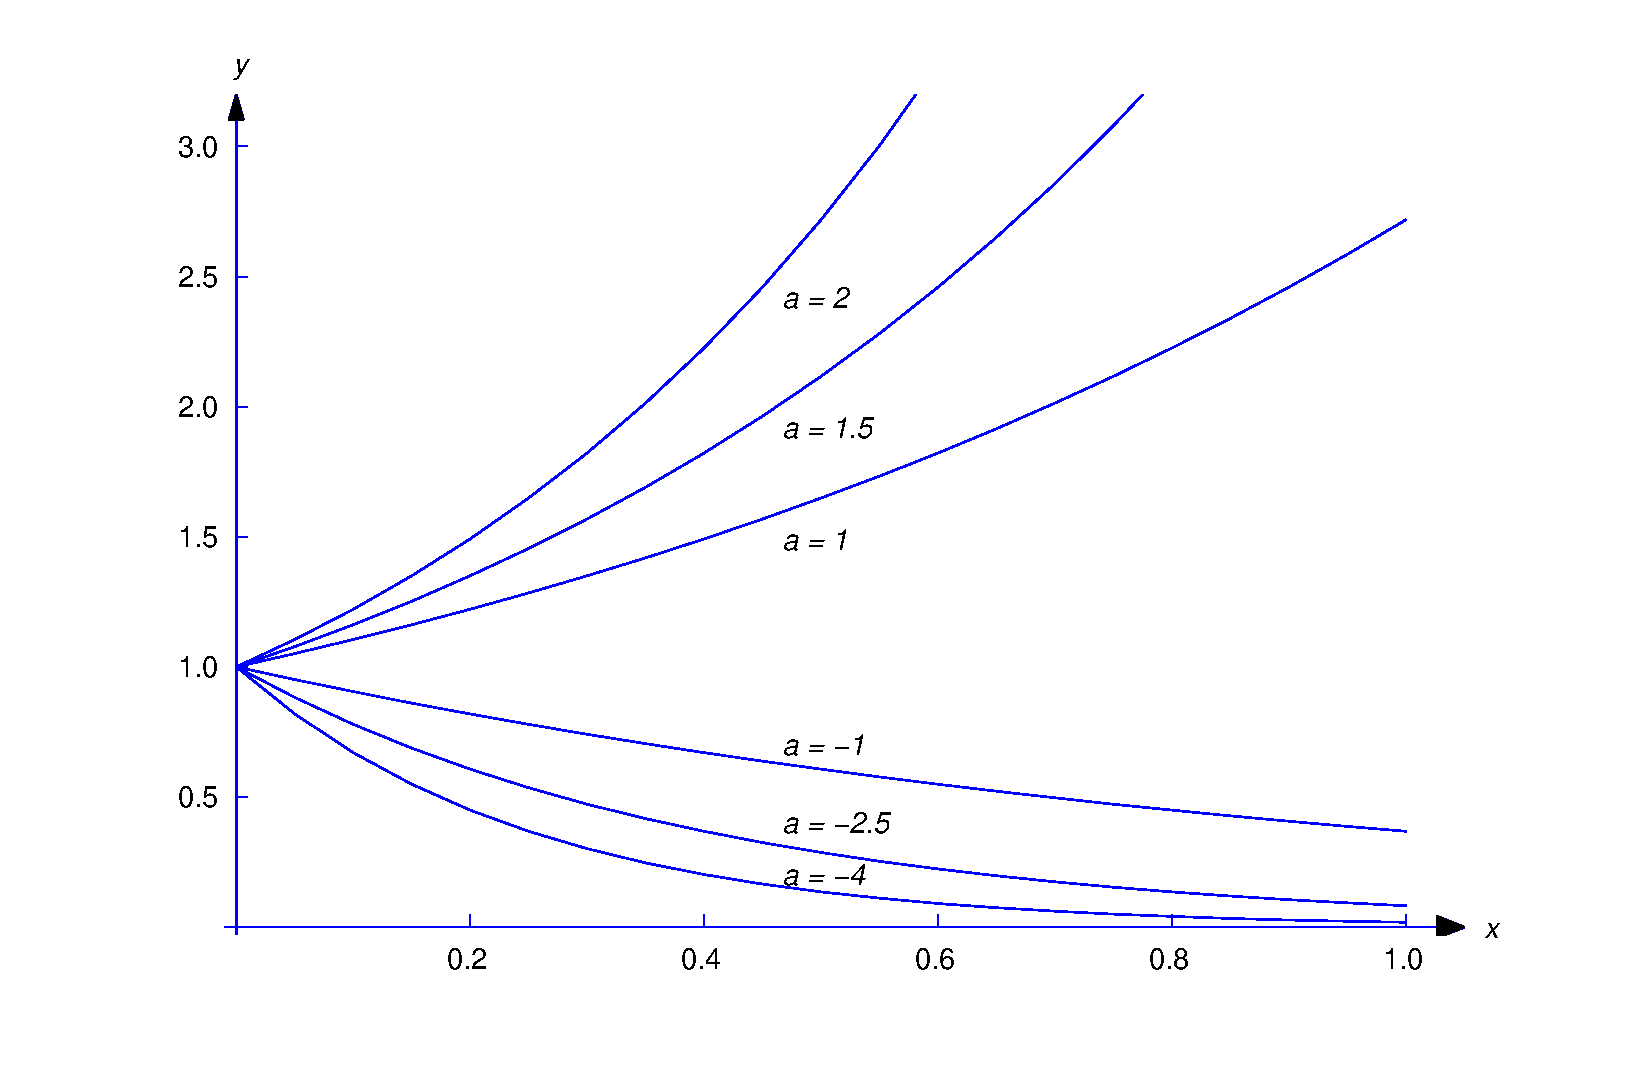
\includegraphics[bb=-78 148 689 643, width=5.67in, height=3.66in, keepaspectratio]{fig020101}
  \relax
  \caption{Solutions of $y'-ay=0$, $y(0)=1$}
  \label{figure:2.1.1}
\end{figure}
\end{examplesolution}

\setcounter{example}{3}
\setcounter{equation}{7}
\begin{example}
  \label{example:2.1.4}\rm

  \begin{alist}
    \item % (a)
    Find the general solution of
    \begin{equation}
      xy'+y=0.\label{eq:2.1.8}
    \end{equation}

    \item % (b)
    Solve the initial value problem
    \begin{equation}
      xy'+y=0,\quad y(1)=3.\label{eq:2.1.9}
    \end{equation}
  \end{alist}
\end{example}
\setcounter{equation}{9}
\setcounter{figure}{1}
\begin{examplesolution}
\solutionpart{a} We rewrite \eqref{eq:2.1.8} as
\begin{equation}
  \label{eq:2.1.10}y'+\frac{1}{x}y=0,
\end{equation}
where $x$ is restricted to either $(-\infty,0)$ or $(0,\infty)$. If $y$ is a nontrivial solution of
\eqref{eq:2.1.10}, there must be some open interval I on which $y$ has no zeros. We can rewrite
\eqref{eq:2.1.10} as
\[
  \frac{y'}{y}=-\frac{1}{x}
\]
for $x$ in $I$. Integrating shows that
\[
  \ln|y|=-\ln|x|+k,\mbox{\quad so\quad}|y|=\frac{e^{k}}{|x|}.
\]
Since a function that satisfies the last equation can't change sign on either $(-\infty,0)$ or
$(0,\infty)$, we can rewrite this result more simply as
\begin{equation}
  \label{eq:2.1.11}y=\frac{c}{x}
\end{equation}
where
\[
  c=\left\{
  \begin{array}{cl}
    \phantom{-}e^{k} & \mbox{if }y>0, \\
    -e^{k}           & \mbox{if }y<0.
  \end{array}\right.
\]
We've now shown that every solution of \eqref{eq:2.1.10} is given by \eqref{eq:2.1.11} for some
choice of $c$. (Even though we assumed that $y$ was nontrivial to derive \eqref{eq:2.1.11}, we can
get the trivial solution by setting $c=0$ in \eqref{eq:2.1.11}.) Conversely, any function of the
form \eqref{eq:2.1.11} is a solution of \eqref{eq:2.1.10}, since differentiating \eqref{eq:2.1.11}
yields
\[
  y'=-\frac{c}{x^{2}},
\]
and substituting this and \eqref{eq:2.1.11} into \eqref{eq:2.1.10} yields
\begin{eqnarray*}
  y'+\frac{1}{x}y & = & -\frac{c}{x^{2}}+\frac{1}{x}\frac{c}{x} \\[2\jot]
                  & = & -\frac{c}{x^{2}}+\frac{c}{x^{2}}=0.
\end{eqnarray*}

Figure~\ref{figure:2.1.2} shows the graphs of some solutions corresponding to various values of $c$. \solutionpart{b} Imposing the initial condition $y(1)=3$ in \eqref{eq:2.1.11} yields $c=3$.
Therefore the solution of \eqref{eq:2.1.9} is
\[
  y=\frac{3}{x}.
\]
The interval of validity of this solution is $(0,\infty)$.

\begin{figure}[H]
  \centering
  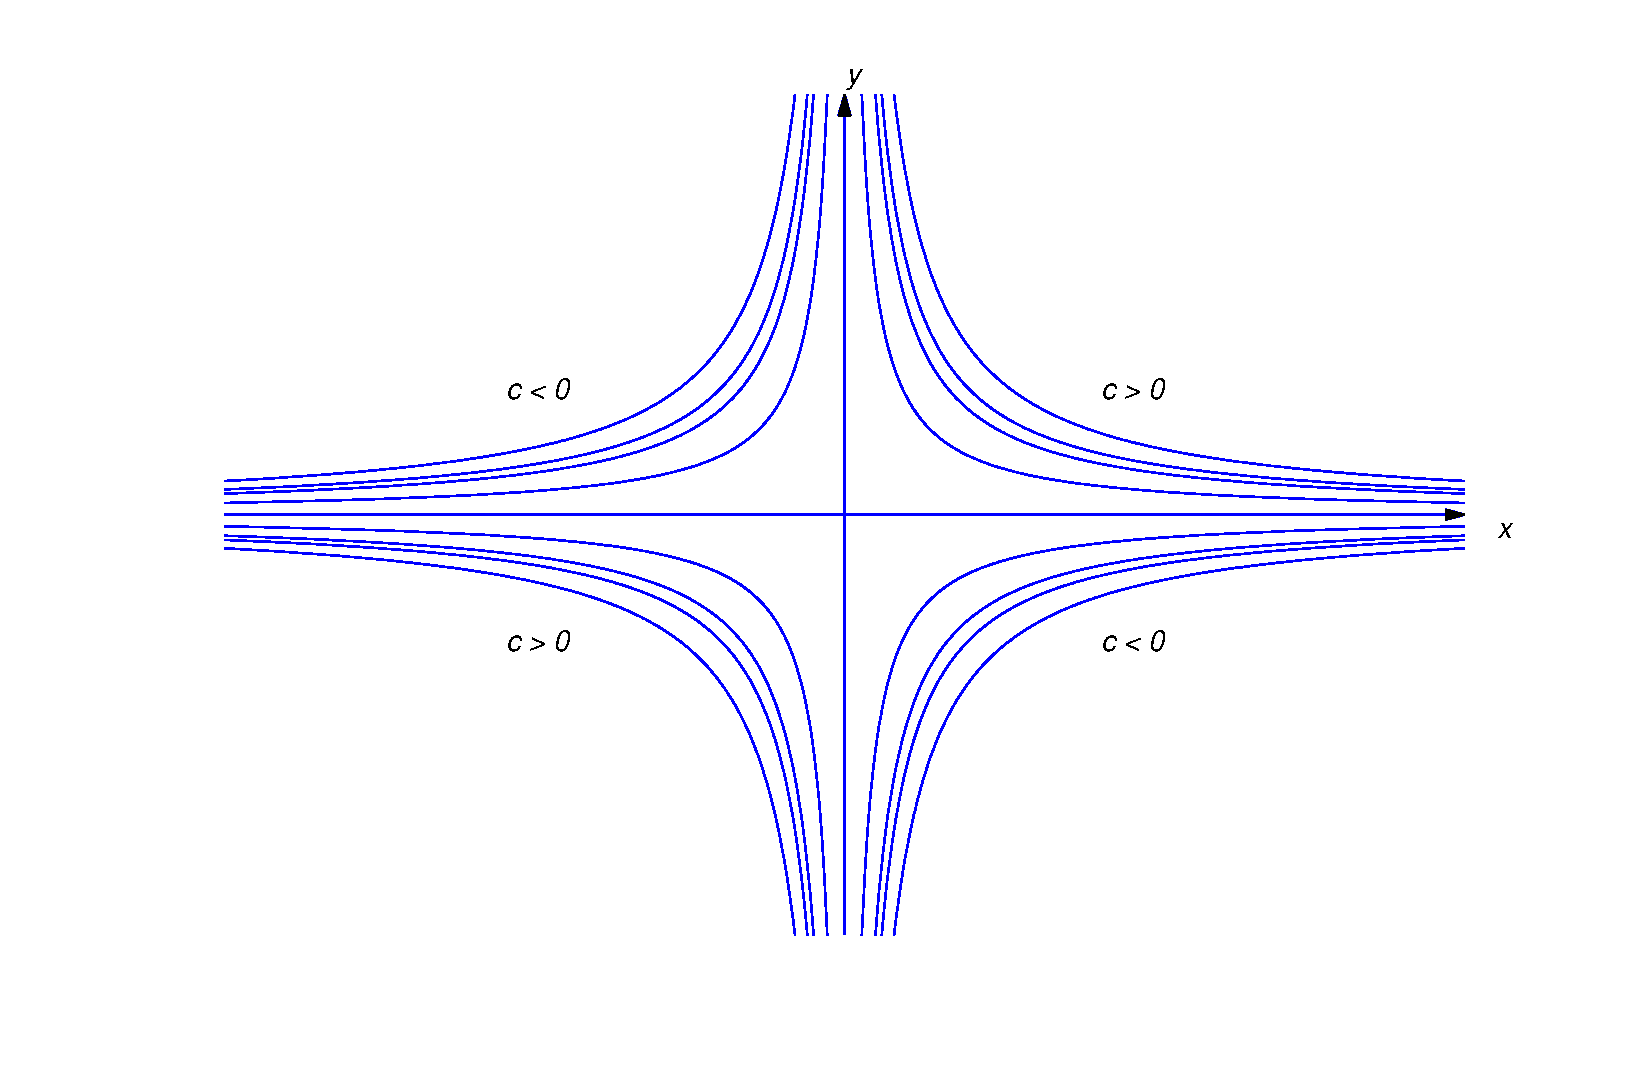
\includegraphics[bb=-78 148 689 643, width=5.67in, height=3.66in, keepaspectratio]{fig020102}
  \relax
  \caption{Solutions of $xy'+y=0$ on $(0,\infty)$ and $(-\infty,0)$}
  \label{figure:2.1.2}
\end{figure}
\end{examplesolution}

\setcounter{example}{4}
\setcounter{equation}{17}
\begin{example}
  \label{example:2.1.5}\rm Find the general solution of
  \begin{equation}
    \label{eq:2.1.18}y'+2y=x^{3}e^{-2x}.
  \end{equation}
\end{example}
\setcounter{equation}{18}
\setcounter{figure}{2}
\begin{examplesolution}
\solution By applying \part{a} of Example~ \ref{example:2.1.3} with $a=-2$, we see that $y_{1}=e^{-2x}$ is a
solution of the complementary equation $y'+2y=0$. Therefore we seek solutions of \eqref{eq:2.1.18}
in the form $y=ue^{-2x}$, so that
\begin{equation}
  \label{eq:2.1.19}y'=u'e^{-2x}-2ue^{-2x}\mbox{\quad and \quad }y'+2y=u'e^{-2x}-2ue^{-2x}+2ue^{-2x}=u'e^{-2x}.
\end{equation}
Therefore $y$ is a solution of \eqref{eq:2.1.18} if and only if
\[
  u'e^{-2x}=x^{3}e^{-2x}\mbox{\quad or, equivalently,\quad}u'=x^{3}.
\]
Therefore
\[
  u=\frac{x^{4}}{4}+c,
\]
and
\[
  y=ue^{-2x}=e^{-2x}\left(\frac{x^{4}}{4}+c\right)
\]
is the general solution of \eqref{eq:2.1.18}.

Figure~\ref{figure:2.1.3} shows a direction field and some integral curves for \eqref{eq:2.1.18}.

\begin{figure}[H]
  \centering
  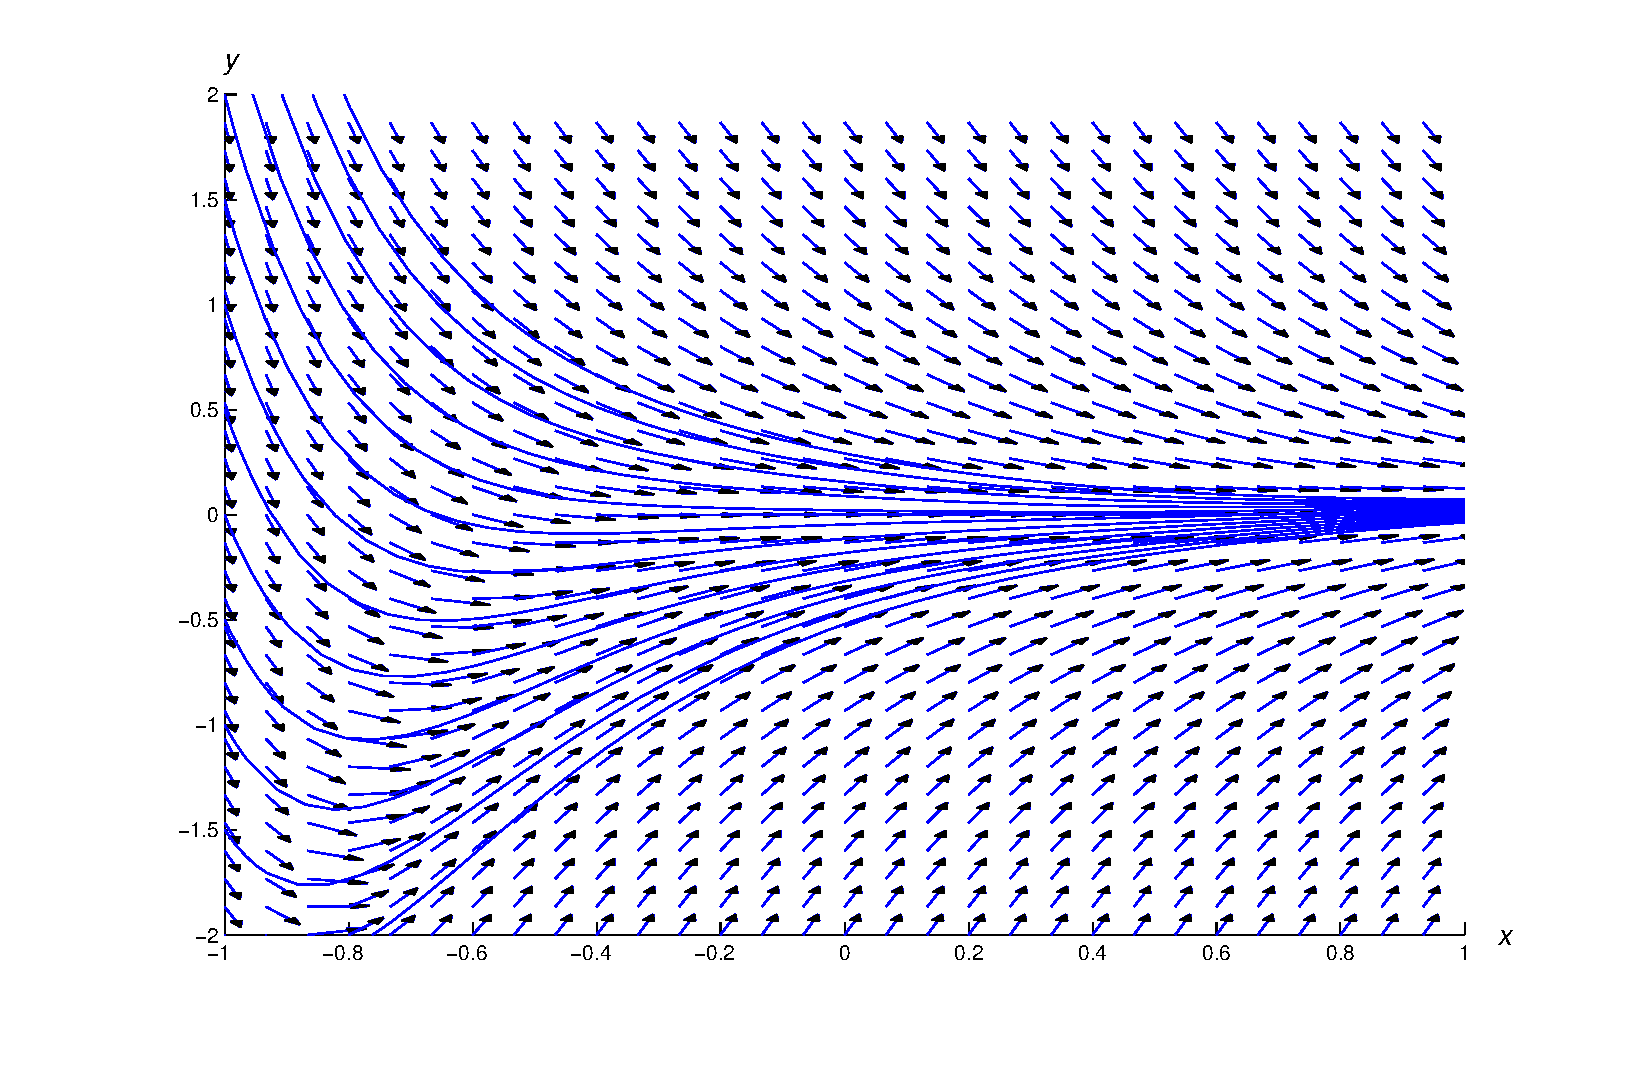
\includegraphics[bb=-78 148 689 643, width=5.67in, height=3.66in, keepaspectratio]{fig020103}
  \relax
  \caption{A direction field and integral curves for $y'+2y=x^{3}e^{-2x}$}
  \label{figure:2.1.3}
\end{figure}
\end{examplesolution}

\setcounter{example}{5}
\setcounter{equation}{19}
\begin{example}
  \label{example:2.1.6}\rm\mbox{}%\newline
  \begin{alist}
    \item % (a)
    Find the general solution
    of \begin{equation}
      \label{eq:2.1.20}y'+(\cot x)y=x\csc x.
    \end{equation}

    \item % (b)
    Solve the initial value problem
    \begin{equation}
      \label{eq:2.1.21}y'+(\cot x)y=x\csc x,\quad y(\pi/2)=1.
    \end{equation}
  \end{alist}
\end{example}
\setcounter{equation}{21}
\setcounter{figure}{3}
\begin{examplesolution}
\solutionpart{a} Here $p(x)=\cot x$ and $f(x)=x\csc x$ are both continuous except at the points
$x=r\pi$, where $r$ is an integer. Therefore we seek solutions of \eqref{eq:2.1.20} on the intervals
$\left(r\pi,(r+1)\pi\right)$. We need a nontrivial solution $y_{1}$ of the complementary equation;
thus, $y_{1}$ must satisfy $y_{1}'+(\cot x)y_{1}=0$, which we rewrite as
\begin{equation}
  \label{eq:2.1.22}\frac{y_{1}'}{y_{1}}=-\cot x=-\frac{\cos x}{\sin x}.
\end{equation}
Integrating this yields
\[
  \ln|y_{1}|=-\ln|\sin x|,
\]
where we take the constant of integration to be zero since we need only {\relax\it one\/}
function that satisfies \eqref{eq:2.1.22}. Clearly $y_{1}=1/\sin x$ is a suitable choice. Therefore
we seek solutions of \eqref{eq:2.1.20} in the form
\[
  y=\frac{u}{\sin x},
\]
so that
\begin{equation}
  \label{eq:2.1.23}y'=\frac{u'}{\sin x}-\frac{u\cos x}{\sin^{2}x}
\end{equation}
and
\begin{equation}
  \label{eq:2.1.24}
  \begin{array}{rcl}
    y'+(\cot x)y & = & \dst\frac{u'}{\sin x}-\dst\frac{u\cos x}{\sin^{2}x}+\dst\frac{u\cot x}{\sin x}    \\[2\jot]
                 & = & \dst\frac{u'}{\sin x}-\dst\frac{u\cos x}{\sin^{2}x}+\dst\frac{u\cos x}{\sin^{2}x} \\[2\jot]
                 & = & \dst\frac{u'}{\sin x}.
  \end{array}
\end{equation}
Therefore $y$ is a solution of \eqref{eq:2.1.20} if and only if
\[
  u'/\sin x=x\csc x=x/\sin x\mbox{\quad or, equivalently, \quad}u'=x.
\]
Integrating this yields
\begin{equation}
  \label{eq:2.1.25}u=\frac{x^{2}}{2}+c,\text{\quad and \quad }y=\frac{u}{\sin x}=\frac{x^{2}}{2\sin x}+\frac{c}{\sin x}
\end{equation}
is the general solution of \eqref{eq:2.1.20} on every interval $\left(r\pi,(r+1)\pi\right)$
($r=$integer).

\solutionpart{b} Imposing the initial condition $y(\pi/2)=1$ in \eqref{eq:2.1.25} yields
\[
  1=\frac{\pi^{2}}{8}+c\mbox{\quad or\quad}c=1-\frac{\pi^{2}}{8}.
\]
Thus,
\[
  y=\frac{x^{2}}{2\sin x}+\frac{(1-\pi^{2}/8)}{\sin x}
\]
is a solution of \eqref{eq:2.1.21}. The interval of validity of this solution is $(0,\pi)$;
Figure~\ref{figure:2.1.4} shows its graph.

\begin{figure}[H]
  \centering
  \scalebox{.8}{
  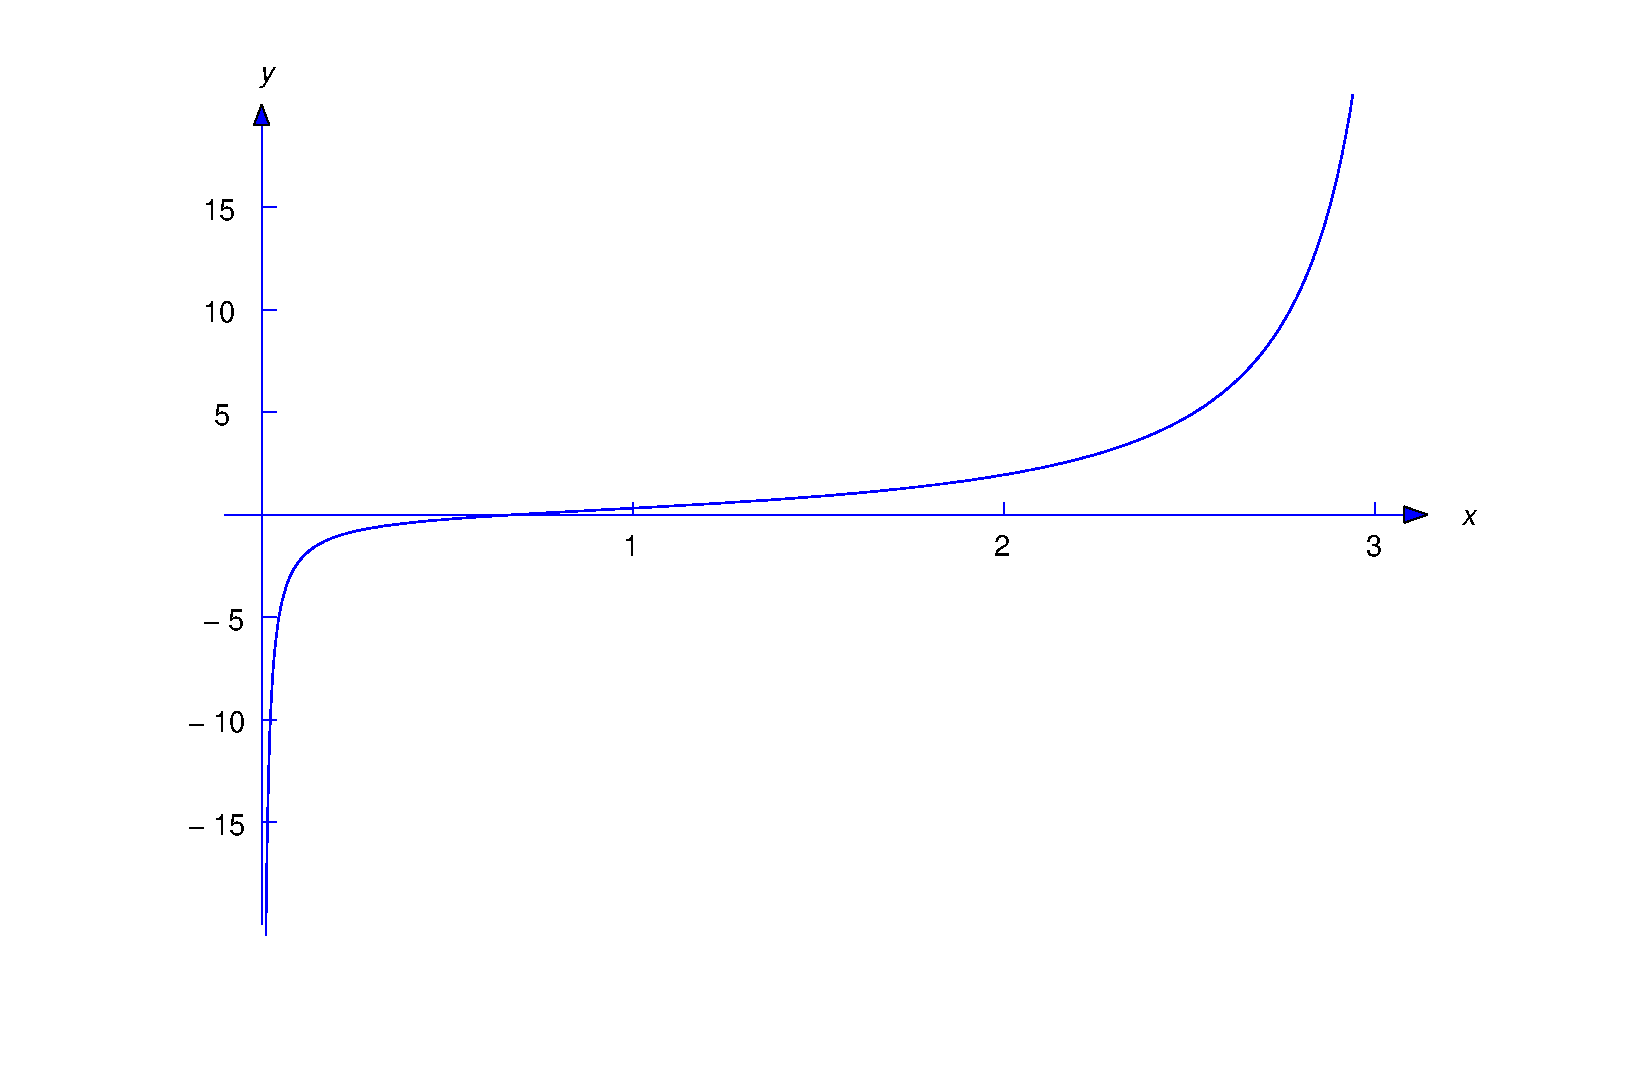
\includegraphics[bb=-78 148 689 643, width=5.67in, height=3.66in, keepaspectratio]{fig020104}}
  \relax
  \caption{Solution of $y'+(\cot x)y=x\csc x$, $y(\pi/2)=1$}
  \label{figure:2.1.4}
\end{figure}

\relax
\remark{It wasn't necessary to do the computations \eqref{eq:2.1.23} and \eqref{eq:2.1.24} in
Example~\ref{example:2.1.6}, since we showed in the discussion preceding Example~\ref{example:2.1.5}
that if $y=uy_{1}$ where $y_{1}'+p(x)y_{1}=0$, then $y'+p(x)y=u'y_{1}$. We did these computations so
you would see this happen in this specific example. We recommend that you include these
``unnecessary'' computations in doing exercises, until you're confident that you really understand
the method. After that, omit them.}
\color{black}
\end{examplesolution}

\setcounter{example}{6}
\setcounter{equation}{27}
\begin{example}
  \label{example:2.1.7}\rm \mbox{}
  \newline
  \begin{alist}
    \item % (a)
    Find the general solution of
    \[
      y'-2xy=1.
    \]

    \item % (b)
    Solve the initial value problem
    \begin{equation}
      \label{eq:2.1.28}y'-2xy=1,\quad y(0)=y_{0}.
    \end{equation}
  \end{alist}
\end{example}
\setcounter{equation}{28}
\setcounter{figure}{4}
\begin{examplesolution}
\solutionpart{a} To apply variation of parameters, we need a nontrivial solution $y_{1}$ of the
complementary equation; thus, $y_{1}'-2xy_{1}=0$, which we rewrite as
\[
  \frac{y_{1}'}{y_{1}}=2x.
\]
Integrating this and taking the constant of integration to be zero yields
\[
  \ln|y_{1}|=x^{2},\mbox{\quad so \quad}|y_{1}|=e^{x^{2}}.
\]
We choose $y_{1}=e^{x^{2}}$ and seek solutions of \eqref{eq:2.1.28} in the form $y=ue^{x^{2}}$,
where
\[
  u'e^{x^{2}}=1,\mbox{\quad so \quad}u'=e^{-x^{2}}.
\]
Therefore
\[
  u=c+\int e^{-x^{2}}dx,
\]
but we can't simplify the integral on the right because there's no elementary function with
derivative equal to $e^{-x^{2}}$. Therefore the best available form for the general solution of
\eqref{eq:2.1.28} is
\begin{equation}
  \label{eq:2.1.29}y=ue^{x^{2}}=e^{x^{2}}\left(c+\int e^{-x^{2}}dx\right).
\end{equation}

\solutionpart{b} Since the initial condition in \eqref{eq:2.1.28} is imposed at $x_{0}=0$, it is
convenient to rewrite \eqref{eq:2.1.29} as
\[
  y=e^{x^{2}}\left(c+\int^{x}_{0}e^{-t^{2}}dt\right),\mbox{\quad since \quad}\int_{0}^{0}e^{-t^{2}}\,dt=0.
\]
Setting $x=0$ and $y=y_{0}$ here shows that $c=y_{0}$. Therefore the solution of the initial value
problem is
\begin{equation}
  \label{eq:2.1.30}y=e^{x^{2}}\left(y_{0}+\int^{x}_{0}e^{-t^{2}}dt\right).
\end{equation}
For a given value of $y_{0}$ and each fixed $x$, the integral on the right can be evaluated by
numerical methods. An alternate procedure is to apply the numerical integration procedures discussed
in Chapter~3 directly to the initial value problem \eqref{eq:2.1.28}. Figure~\ref{figure:2.1.5}
shows graphs of \eqref{eq:2.1.30} for several values of $y_{0}$.

\begin{figure}[H]
  \centering
  \scalebox{.9}{
  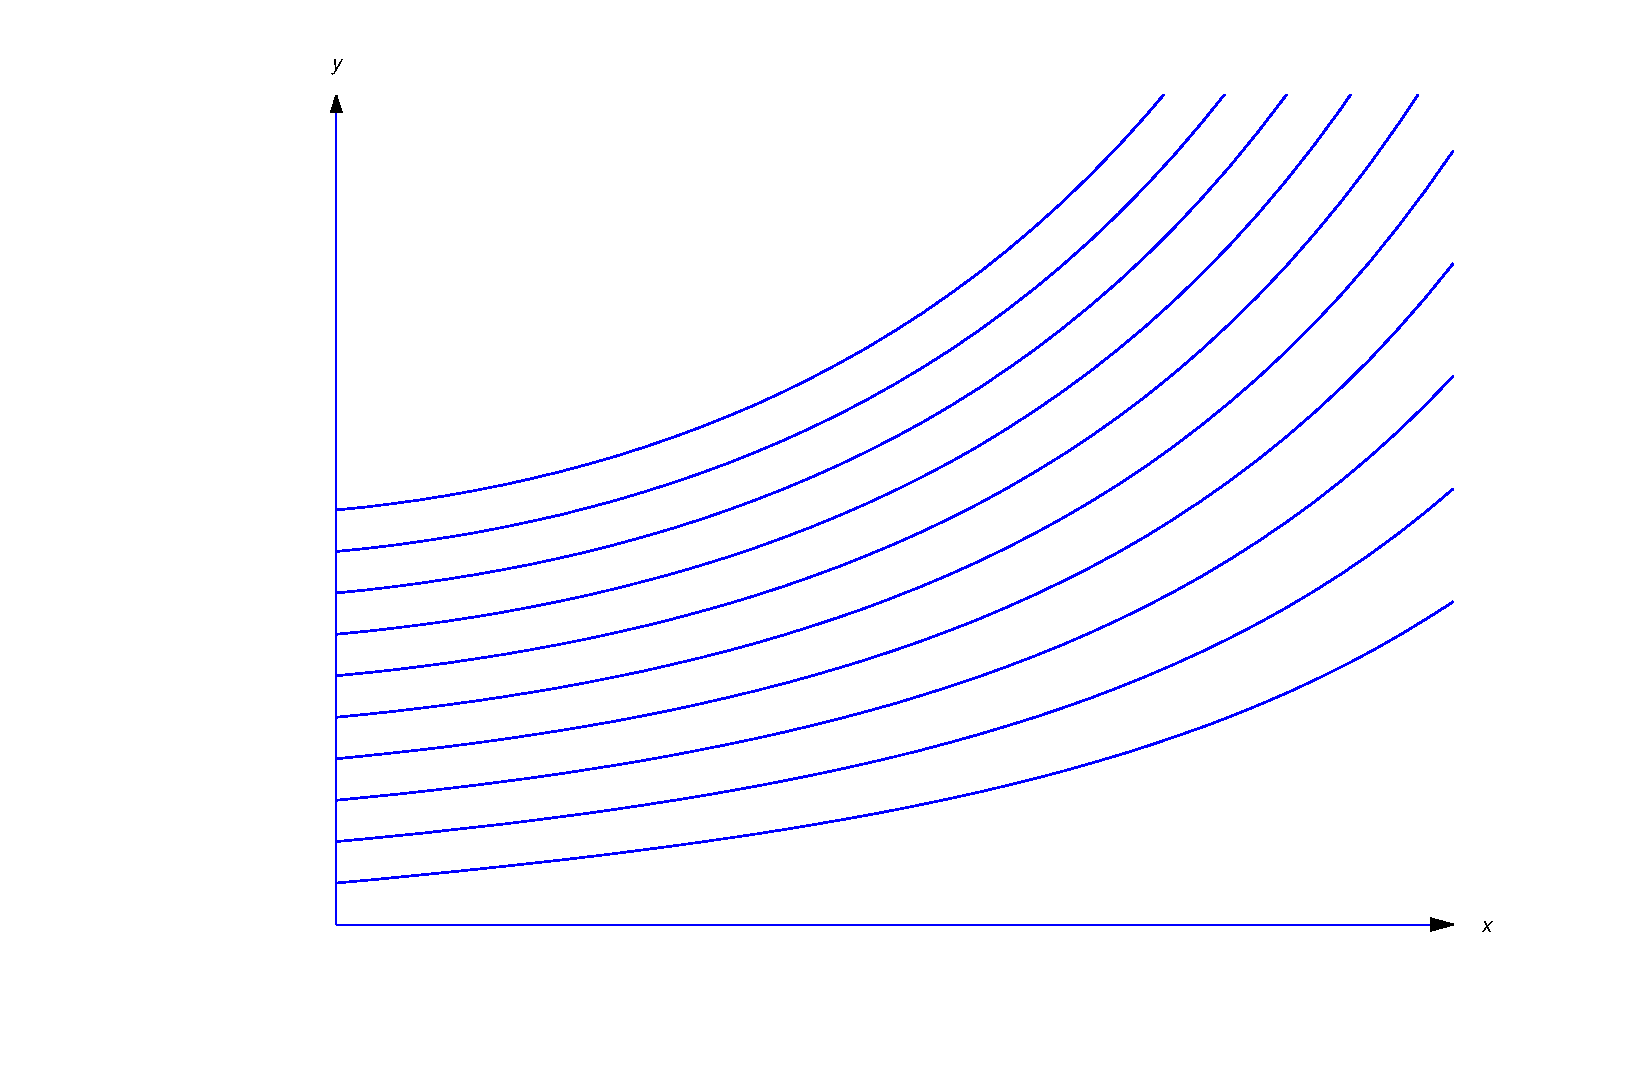
\includegraphics[bb=-78 148 689 643, width=5.67in, height=3.66in, keepaspectratio]{fig020105}
  }
  \relax
  \caption{Solutions of $y'-2xy=1$, $y(0)=y_{0}$}
  \label{figure:2.1.5}
\end{figure}
\end{examplesolution}

\section*{Section 2.2}
\setcounter{chapter}{2}
\setcounter{section}{2}

\setcounter{example}{0}
\begin{example}
  \label{example:2.2.1}\rm Solve the equation
  \[
    y'=x(1+y^{2}).
  \]
\end{example}
\begin{examplesolution}
\solution Separating variables yields
\[
  \frac{y'}{1+y^{2}}=x.
\]
Integrating yields
\[
  \tan^{-1}y=\frac{x^{2}}{2}+c
\]
Therefore
\[
  y=\tan\left(\frac{x^{2}}{2}+c\right).
\]
\end{examplesolution}

\setcounter{example}{1}
\setcounter{equation}{3}
\begin{example}
  \label{example:2.2.2} \rm \mbox{}
  \newline
  \begin{alist}
    \item % (a)
    Solve the equation
    \begin{equation}
      \label{eq:2.2.4}y'=-\frac{x}{y}.
    \end{equation}

    \item % (b)
    Solve the initial value problem
    \begin{equation}
      \label{eq:2.2.5}y'=-\frac{x}{y},\quad y(1)=1.
    \end{equation}

    \item % (c)
    Solve the initial value problem
    \begin{equation}
      \label{eq:2.2.6}y'=-\frac{x}{y},\quad y(1)=-2.
    \end{equation}
  \end{alist}
\end{example}
\setcounter{equation}{6}
\setcounter{figure}{0}
\begin{examplesolution}
\solutionpart{a} Separating variables in \eqref{eq:2.2.4} yields
\[
  yy'=-x.
\]
Integrating yields
\[
  \frac{y^{2}}{2}=-\frac{x^{2}}{2}+c,\mbox{\quad or,\, equivalently, \quad}x^{2}+y^{2}=2c.
\]
The last equation shows that $c$ must be positive if $y$ is to be a solution of \eqref{eq:2.2.4} on
an open interval. Therefore we let $2c=a^{2}$ (with $a>0$) and rewrite the last equation as
\begin{equation}
  \label{eq:2.2.7}x^{2}+y^{2}=a^{2}.
\end{equation}
This equation has two differentiable solutions for $y$ in terms of $x$:
\begin{equation}
  \label{eq:2.2.8}y=\phantom{-}\sqrt{a^{2}-x^{2}},\quad-a<x<a,
\end{equation}
and
\begin{equation}
  \label{eq:2.2.9}y=-\sqrt{a^{2}-x^{2}},\quad-a<x<a.
\end{equation}
The solution curves defined by \eqref{eq:2.2.8} are semicircles above the $x$-axis and those defined
by \eqref{eq:2.2.9} are semicircles below the $x$-axis (Figure~\ref{figure:2.2.1}).

\solutionpart{b} The solution of \eqref{eq:2.2.5} is positive when $x=1$; hence, it is of the form
\eqref{eq:2.2.8}. Substituting $x=1$ and $y=1$ into \eqref{eq:2.2.7} to satisfy the initial
condition yields $a^{2}=2$; hence, the solution of \eqref{eq:2.2.5} is
\[
  y=\sqrt{2-x^{2}},\quad-\sqrt{2}<x<\sqrt{2}.
\]

\solutionpart{c} The solution of \eqref{eq:2.2.6} is negative when $x=1$ and is therefore of the
form \eqref{eq:2.2.9}. Substituting $x=1$ and $y=-2$ into \eqref{eq:2.2.7} to satisfy the initial
condition yields $a^{2}=5$. Hence, the solution of \eqref{eq:2.2.6} is
\[
  y=-\sqrt{5-x^{2}},\quad-\sqrt{5}<x<\sqrt{5}.
\]

\begin{figure}[H]
  \centering
  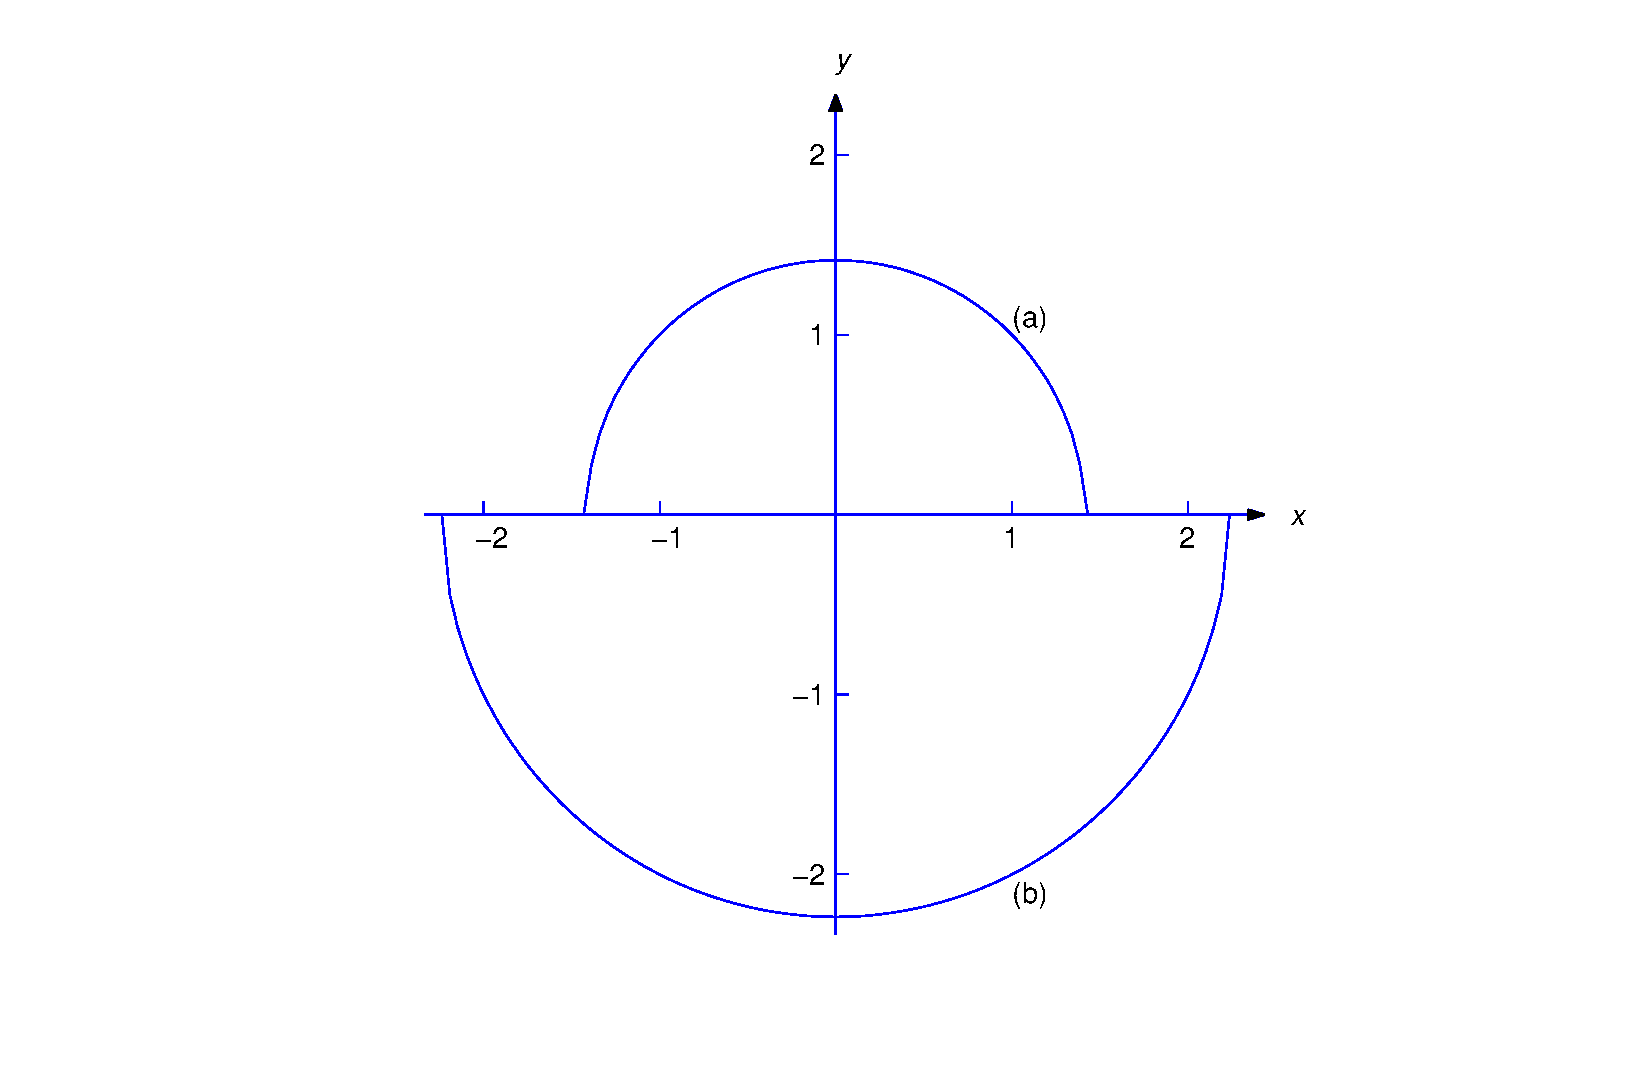
\includegraphics[bb=-78 148 689 643, width=5.67in, height=3.66in, keepaspectratio]{fig020201}
  \relax
  \caption{{\bf (a)} $y=\sqrt{2-x^{2}}$,\, $-\sqrt{2}<x<\sqrt{2}$; \, {\bf (b)} $y=-\sqrt{5-x^{2}}$,\, $-\sqrt{5}<x<\sqrt{5}$}
  \label{figure:2.2.1}
\end{figure}
\end{examplesolution}

\setcounter{example}{2}
\setcounter{equation}{12}
\begin{example}
  \label{example:2.2.3} \rm \mbox{}
  \newline
  \begin{alist}
    \item % (a)
    Find implicit solutions of
    \begin{equation}
      \label{eq:2.2.13}y'=\frac{2x+1}{5y^{4}+1}.
    \end{equation}

    \item % (b)
    Find an implicit solution of
    \begin{equation}
      \label{eq:2.2.14}y'=\frac{2x+1}{5y^{4}+1},\quad y(2)=1.
    \end{equation}
  \end{alist}
\end{example}
\setcounter{equation}{14}
\setcounter{figure}{1}
\begin{examplesolution}
\solutionpart{a} Separating variables yields
\[
  (5y^{4}+1)y'=2x+1.
\]
Integrating yields the implicit solution
\begin{equation}
  \label{eq:2.2.15}y^{5}+y=x^{2}+x+c
\end{equation}
of \eqref{eq:2.2.13}.

\solutionpart{b} Imposing the initial condition $y(2)=1$ in \eqref{eq:2.2.15} yields $1+1=4+2+c$, so
$c=-4$. Therefore
\[
  y^{5}+y=x^{2}+x-4
\]
is an implicit solution of the initial value problem \eqref{eq:2.2.14}. Although more than one
differentiable function $y=y(x)$ satisfies \eqref{eq:2.2.15} near $x=2$, it can be shown that there's
only one such function that satisfies the initial condition $y(2)=1$.

Figure~\ref{figure:2.2.2} shows a direction field and some integral curves for \eqref{eq:2.2.13}.

\begin{figure}[H]
  \centering
  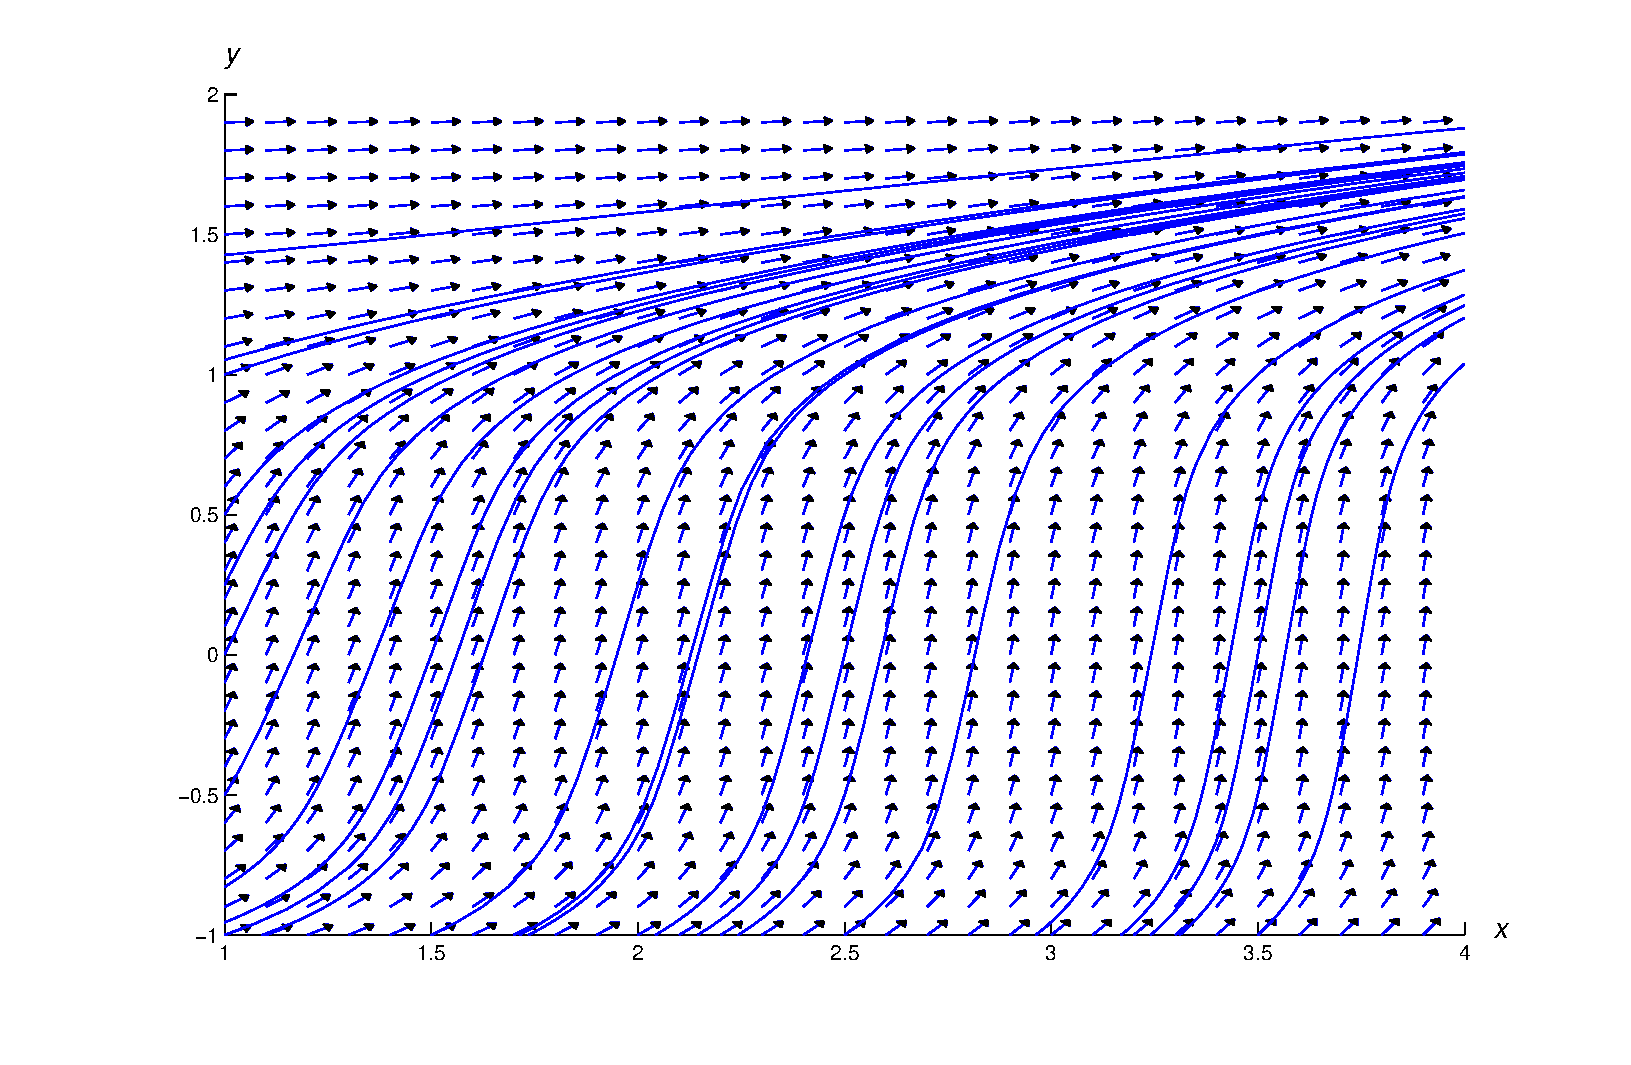
\includegraphics[bb=-78 148 689 643, width=5.67in, height=3.66in, keepaspectratio]{fig020202}
  \relax
  \caption{A direction field and integral curves for $y'=\dst{\frac{2x+1}{5y^{4}+1}}$}
  \label{figure:2.2.2}
\end{figure}
\end{examplesolution}

\setcounter{example}{3}
\setcounter{equation}{15}
\begin{example}
  \label{example:2.2.4} \rm Find all solutions of
  \begin{equation}
    \label{eq:2.2.16}y'=2xy^{2}.
  \end{equation}
\end{example}
\setcounter{equation}{16}
\setcounter{figure}{2}
\begin{examplesolution}
\solution Here we must divide by $p(y)=y^{2}$ to separate variables. This isn't legitimate if $y$ is
a solution of \eqref{eq:2.2.16} that equals zero for some value of $x$. One such solution can be
found by inspection: $y\equiv0$. Now suppose $y$ is a solution of \eqref{eq:2.2.16} that isn't
identically zero. Since $y$ is continuous there must be an interval on which $y$ is never zero.
Since division by $y^{2}$ is legitimate for $x$ in this interval, we can separate variables in
\eqref{eq:2.2.16} to obtain
\[
  \frac{y'}{y^{2}}=2x.
\]
Integrating this yields
\[
  -\frac{1}{y}=x^{2}+c,
\]
which is equivalent to
\begin{equation}
  \label{eq:2.2.17}y=-\frac{1}{x^{2}+c}.
\end{equation}

We've now shown that if $y$ is a solution of \eqref{eq:2.2.16} that is not identically zero, then
$y$ must be of the form \eqref{eq:2.2.17}. By substituting \eqref{eq:2.2.17} into \eqref{eq:2.2.16},
you can verify that \eqref{eq:2.2.17} is a solution of \eqref{eq:2.2.16}. Thus, solutions of
\eqref{eq:2.2.16} are $y\equiv0$ and the functions of the form \eqref{eq:2.2.17}. Note that the
solution $y\equiv0$ isn't of the form \eqref{eq:2.2.17} for any value of $c$.

Figure~\ref{figure:2.2.3} shows a direction field and some integral curves for \eqref{eq:2.2.16}. \begin{figure}[H]
  \centering
  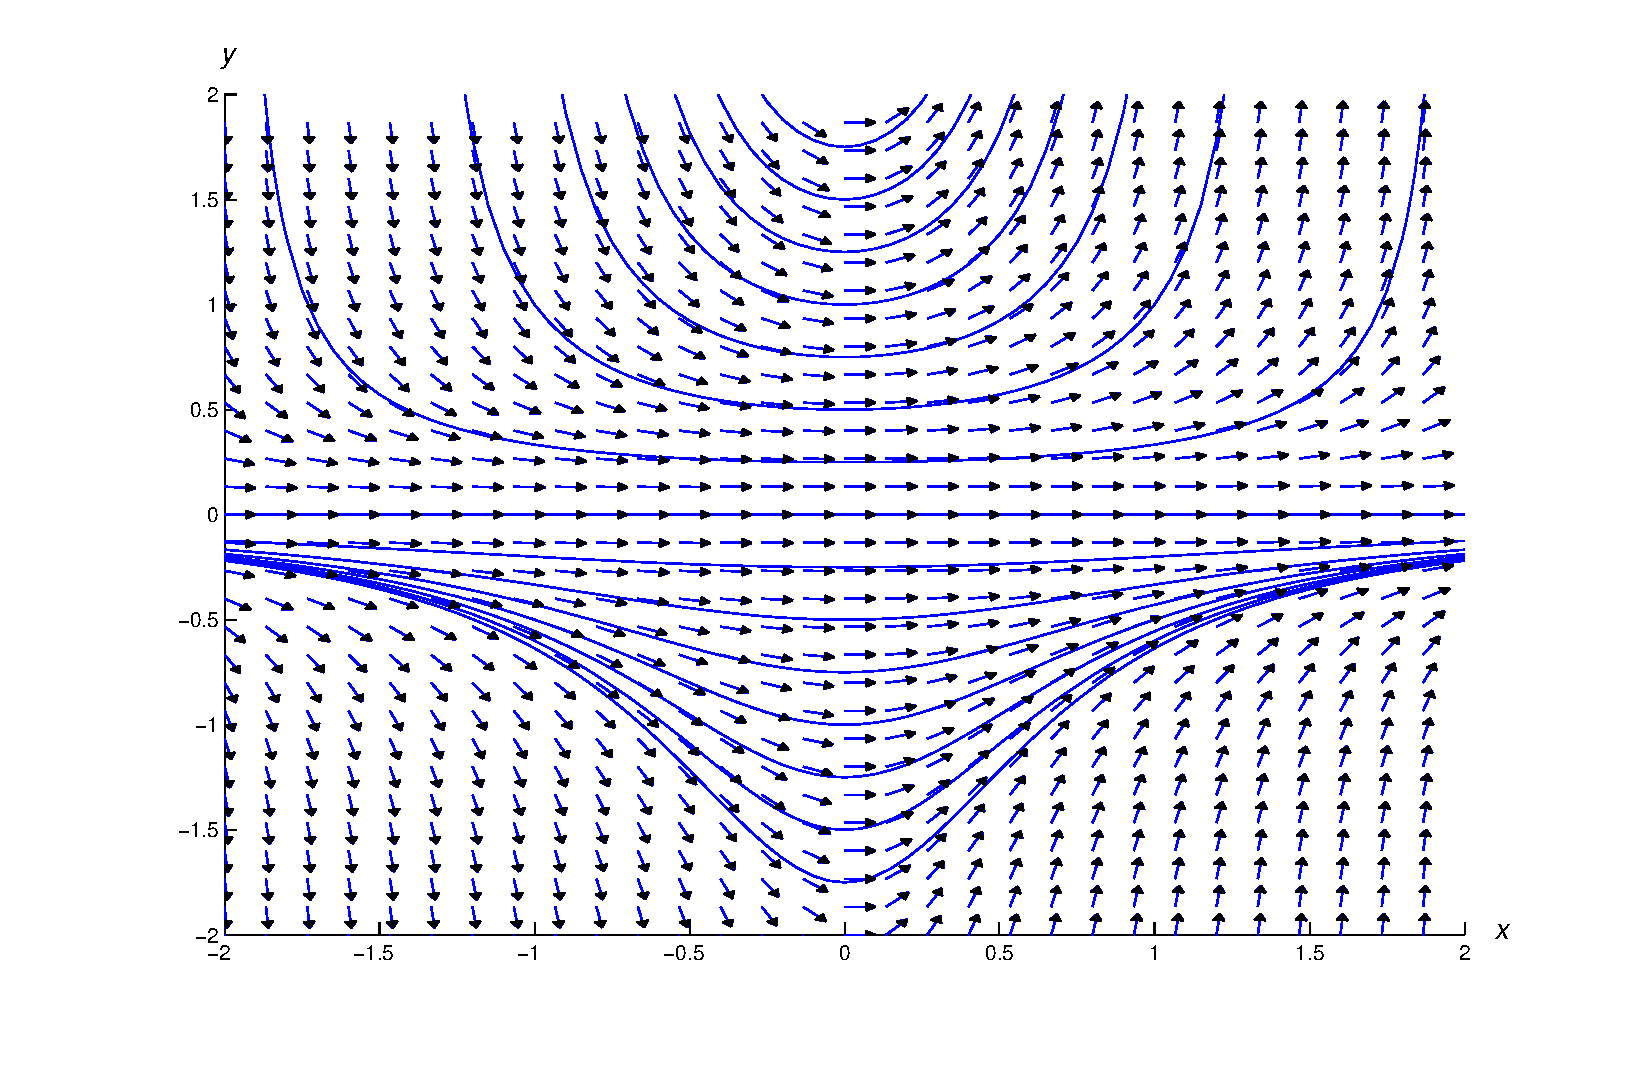
\includegraphics[bb=-78 148 689 643, width=5.67in, height=3.66in, keepaspectratio]{fig020203}
  \relax
  \caption{A direction field and integral curves for $y'=2xy^{2}$}
  \label{figure:2.2.3}
\end{figure}
\end{examplesolution}

\setcounter{example}{4}
\setcounter{equation}{17}
\begin{example}
  \label{example:2.2.5} \rm Find all solutions of
  \begin{equation}
    \label{eq:2.2.18}y'=\frac{1}{2}x(1-y^{2}).
  \end{equation}
\end{example}
\setcounter{equation}{18}
\setcounter{figure}{3}
\begin{examplesolution}
\solution Here we must divide by $p(y)=1-y^{2}$ to separate variables. This isn't legitimate if $y$
is a solution of \eqref{eq:2.2.18} that equals $\pm1$ for some value of $x$. Two such solutions can
be found by inspection: $y\equiv1$ and $y\equiv-1$. Now suppose $y$ is a solution of
\eqref{eq:2.2.18} such that $1-y^{2}$ isn't identically zero. Since $1-y^{2}$ is continuous there
must be an interval on which $1-y^{2}$ is never zero. Since division by $1-y^{2}$ is legitimate for
$x$ in this interval, we can separate variables in \eqref{eq:2.2.18} to obtain
\[
  \frac{2y'}{y^{2}-1}=-x.
\]
A partial fraction expansion on the left yields
\[
  \left[\frac{1}{y-1}-\frac{1}{y+1}\right]y'=-x,
\]
and integrating yields
\[
  \ln\left|\frac{y-1}{y+1}\right|=-\frac{x^{2}}{2}+k;
\]
hence,
\[
  \left|\frac{y-1}{y+1}\right|=e^{k}e^{-x^{2}/2}.
\]
Since $y(x)\ne\pm1$ for $x$ on the interval under discussion, the quantity $(y-1)/(y+1)$ can't
change sign in this interval. Therefore we can rewrite the last equation as
\[
  \frac{y-1}{y+1}=ce^{-x^{2}/2},
\]
where $c=\pm e^{k}$, depending upon the sign of $(y-1)/(y+1)$ on the interval. Solving for $y$
yields
\begin{equation}
  \label{eq:2.2.19}y=\frac{1+ce^{-x^{2}/2}}{1-ce^{-x^{2}/2}}.
\end{equation}

We've now shown that if $y$ is a solution of \eqref{eq:2.2.18} that is not identically equal to
$\pm1$, then $y$ must be as in \eqref{eq:2.2.19}. By substituting \eqref{eq:2.2.19} into
\eqref{eq:2.2.18} you can verify that \eqref{eq:2.2.19} is a solution of \eqref{eq:2.2.18}. Thus,
the solutions of \eqref{eq:2.2.18} are $y\equiv1$, $y\equiv-1$ and the functions of the form
\eqref{eq:2.2.19}. Note that the constant solution $y\equiv1$ can be obtained from this formula by
taking $c=0$; however, the other constant solution, $y\equiv-1$, can't be obtained in this way.

Figure~\ref{figure:2.2.4} shows a direction field and some integral curves for \eqref{eq:2.2.18}.

\begin{figure}[H]
  \centering
  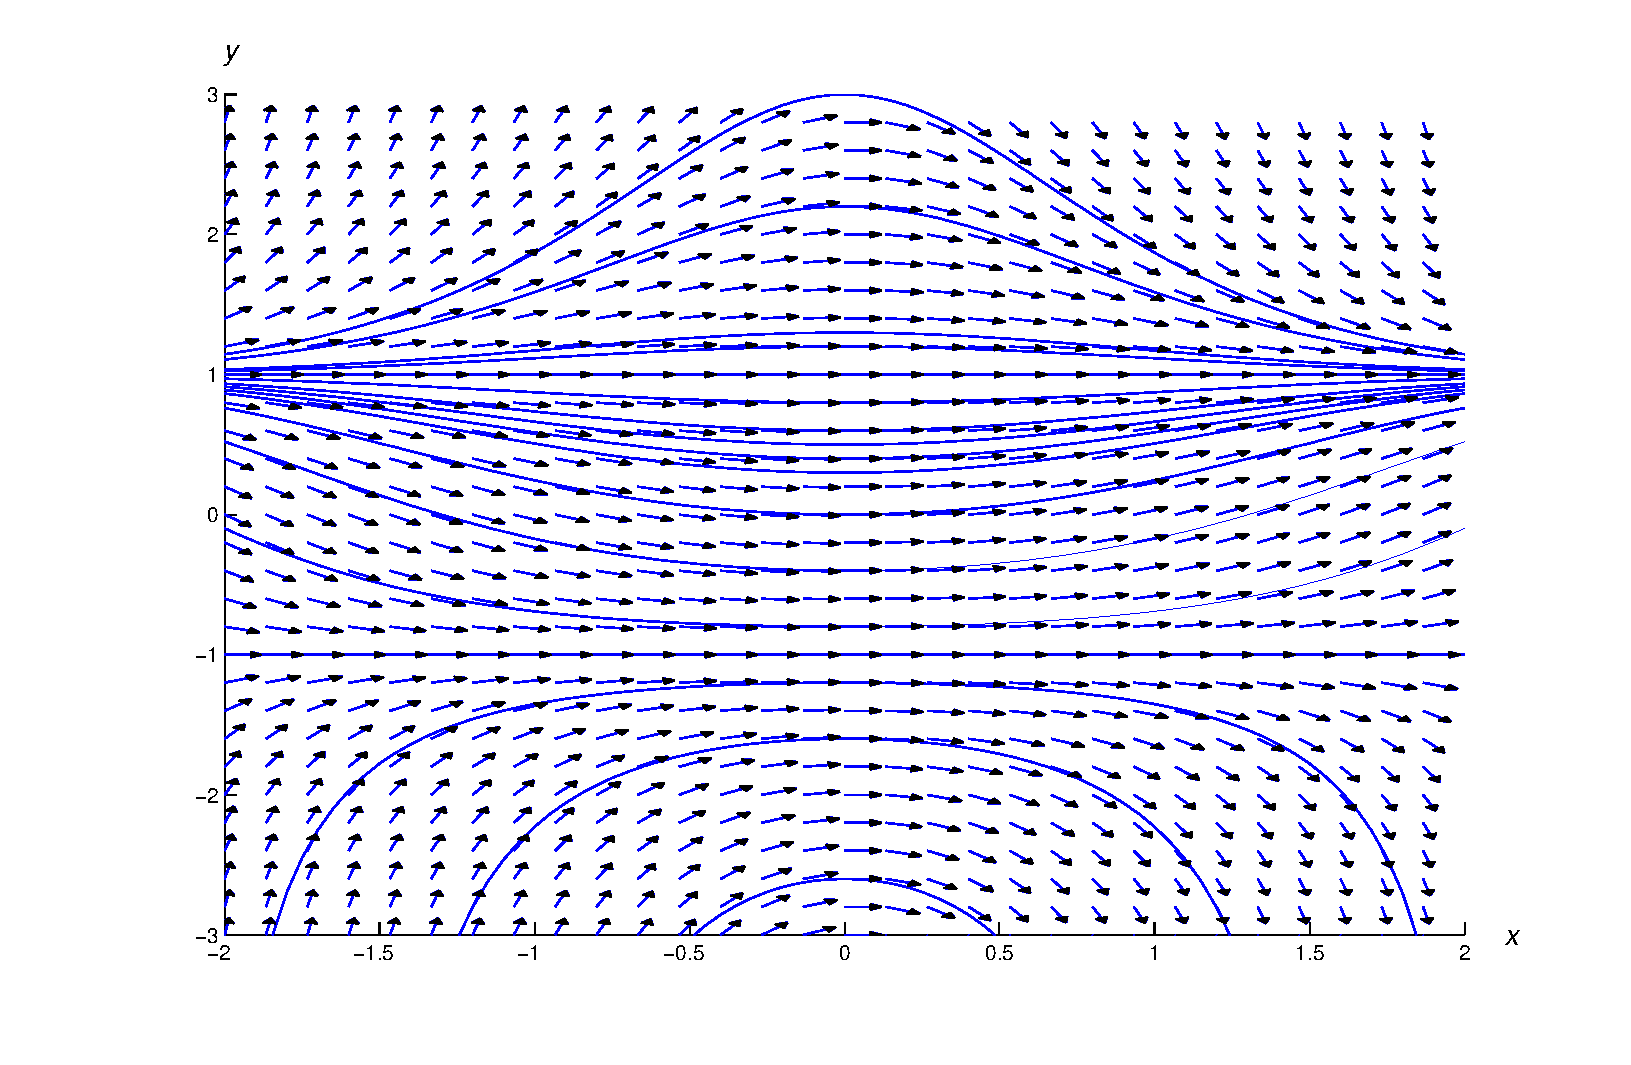
\includegraphics[bb=-78 148 689 643, width=5.67in, height=3.66in, keepaspectratio]{fig020204}
  \relax
  \caption{A direction field and integral curves for $y'=\dst{\frac{x(1-y^{2})}{2}}$}
  \label{figure:2.2.4}
\end{figure}
\end{examplesolution}

\setcounter{example}{5}
\begin{example}
  \label{example:2.2.6} \rm Solve the initial value problem
  \[
    y'=2xy^{2},\quad y(0)=y_{0}
  \]
  and determine the interval of validity of the solution.
\end{example}
\setcounter{equation}{19}
\begin{examplesolution}
\solution First suppose $y_{0}\ne0$. From Example~\ref{example:2.2.4}, we know that $y$ must be of
the form
\begin{equation}
  \label{eq:2.2.20}y=-\frac{1}{x^{2}+c}.
\end{equation}
Imposing the initial condition shows that $c=-1/y_{0}$. Substituting this into \eqref{eq:2.2.20} and
rearranging terms yields the solution
\[
  y=\frac{y_{0}}{1-y_{0}x^{2}}.
\]
This is also the solution if $y_{0}=0$. If $y_{0}<0$, the denominator isn't zero for any value of
$x$, so the solution is valid on $(-\infty,\infty)$. If $y_{0}>0$, the solution is valid only on
$(-1/\sqrt{y_{0}},1/\sqrt{y_{0}})$.
\end{examplesolution}

\section*{Section 2.3}
\setcounter{chapter}{2}
\setcounter{section}{3}

\setcounter{example}{0}
\setcounter{equation}{2}
\begin{example}
  \label{example:2.3.1} \rm Consider the initial value problem
  \begin{equation}
    \label{eq:2.3.3}y'=\frac{x^{2}-y^{2}}{1+x^{2}+y^{2}},\quad y(x_{0})=y_{0}.
  \end{equation}
  Since
  \[
    f(x,y)=\frac{x^{2}-y^{2}}{1+x^{2}+y^{2}}\mbox{\quad and \quad}f_{y}(x,y)=-\frac{2y(1+2x^{2})}{(1+x^{2}+y^{2})^{2}}
  \]
  are continuous for all $(x,y)$, Theorem~2.3.1 implies that if $(x_{0},y_{0})$ is
  arbitrary, then \eqref{eq:2.3.3} has a unique solution on some open interval that contains
  $x_{0}$.
\end{example}

\setcounter{example}{1}
\setcounter{equation}{3}
\begin{example}
  \label{example:2.3.2} \rm Consider the initial value problem
  \begin{equation}
    \label{eq:2.3.4}y'=\frac{x^{2}-y^{2}}{x^{2}+y^{2}},\quad y(x_{0})=y_{0}.
  \end{equation}
  Here
  \[
    f(x,y)=\frac{x^{2}-y^{2}}{x^{2}+y^{2}}\mbox{\quad and \quad}f_{y}(x,y)=\dst-\frac{4x^{2}y}{(x^{2}+y^{2})^{2}}
  \]
  are continuous everywhere except at $(0,0)$. If $(x_{0},y_{0}) \ne(0,0)$, there's an open
  rectangle $R$ that contains $(x_{0},y_{0})$ that does not contain $(0,0)$. Since $f$ and $f_{y}$
  are continuous on $R$, Theorem~2.3.1 implies that if $(x_{0},y_{0})\ne(0,0)$ then
  \eqref{eq:2.3.4} has a unique solution on some open interval that contains $x_{0}$.
\end{example}

\setcounter{example}{2}
\setcounter{equation}{4}
\begin{example}
  \label{example:2.3.3} \rm Consider the initial value problem
  \begin{equation}
    \label{eq:2.3.5}y'=\frac{x+y}{x-y},\quad y(x_{0})=y_{0}.
  \end{equation}
  Here
  \[
    f(x,y)=\frac{x+y}{x-y}\mbox{\quad and \quad}f_{y}(x,y)=\frac{2x}{(x-y)^{2}}
  \]
  are continuous everywhere except on the line $y=x$. If $y_{0}\ne x_{0}$, there's an open rectangle
  $R$ that contains $(x_{0},y_{0})$ that does not intersect the line $y=x$. Since $f$ and $f_{y}$
  are continuous on $R$, Theorem~2.3.1 implies that if $y_{0}\ne x_{0}$,
  \eqref{eq:2.3.5} has a unique solution on some open interval that contains $x_{0}$.
\end{example}

\setcounter{example}{3}
\setcounter{equation}{5}
\begin{example}
  \label{example:2.3.4} \rm In Example~\ref{example:2.2.4} we saw that the solutions of
  \begin{equation}
    \label{eq:2.3.6}y'=2xy^{2}
  \end{equation}
  are
  \[
    y\equiv0\mbox{\quad and \quad}y=-\frac{1}{x^{2}+c},
  \]
  where $c$ is an arbitrary constant. In particular, this implies that no solution of
  \eqref{eq:2.3.6} other than $y\equiv0$ can equal zero for any value of $x$. Show that
  Theorem~2.3.1\part{b} implies this.
\end{example}
\setcounter{equation}{6}
\begin{examplesolution}
\solution We'll obtain a contradiction by assuming that \eqref{eq:2.3.6} has a solution $y_{1}$ that
equals zero for some value of $x$, but isn't identically zero. If $y_{1}$ has this property, there's
a point $x_{0}$ such that $y_{1}(x_{0})=0$, but $y_{1}(x)\ne0$ for some value of $x$ in every open
interval that contains $x_{0}$. This means that the initial value problem
\begin{equation}
  \label{eq:2.3.7}y'=2xy^{2},\quad y(x_{0})=0
\end{equation}
has two solutions $y\equiv0$ and $y=y_{1}$ that differ for some value of $x$ on every open interval
that contains $x_{0}$. This contradicts Theorem~2.3.1(b), since in \eqref{eq:2.3.6}
the functions
\[
  f(x,y)=2xy^{2}\mbox{\quad and \quad}f_{y}(x,y)=4xy
\]
are both continuous for all $(x,y)$, which implies that \eqref{eq:2.3.7} has a unique solution on
some open interval that contains $x_{0}$.
\end{examplesolution}

\setcounter{example}{4}
\setcounter{equation}{7}
\begin{example}
  \label{example:2.3.5} \rm Consider the initial value problem
  \begin{equation}
    \label{eq:2.3.8}y'=\frac{10}{3}xy^{2/5},\quad y(x_{0})=y_{0}.
  \end{equation}
  \begin{alist}
    \item % (a)
    For what points $(x_{0},y_{0})$ does Theorem~2.3.1\part{a} imply that
    \eqref{eq:2.3.8} has a solution?

    \item % (b)
    For what points $(x_{0},y_{0})$ does Theorem~2.3.1\part{b} imply that
    \eqref{eq:2.3.8} has a unique solution on some open interval that contains $x_{0}$?
  \end{alist}
\end{example}
\begin{examplesolution}
\solutionpart{a} Since
\[
  f(x,y)=\frac{10}{3}xy^{2/5}
\]
is continuous for all $(x,y)$, Theorem~2.3.1 implies that \eqref{eq:2.3.8} has a
solution for every $(x_{0},y_{0})$.

\solutionpart{b} Here
\[
  f_{y}(x,y)=\frac{4}{3}xy^{-3/5}
\]
is continuous for all $(x,y)$ with $y\ne0$. Therefore, if $y_{0}\ne0$ there's an open rectangle on
which both $f$ and $f_{y}$ are continuous, and Theorem~2.3.1 implies that
\eqref{eq:2.3.8} has a unique solution on some open interval that contains $x_{0}$.

If $y=0$ then $f_{y}(x,y)$ is undefined, and therefore discontinuous; hence,
Theorem~2.3.1 does not apply to \eqref{eq:2.3.8} if $y_{0}=0$.
\end{examplesolution}

\setcounter{example}{5}
\setcounter{equation}{8}
\begin{example}
  \label{example:2.3.6} \rm Example~\ref{example:2.3.5} leaves open the possibility that the initial
  value problem
  \begin{equation}
    \label{eq:2.3.9}y'=\frac{10}{3}xy^{2/5},\quad y(0)=0
  \end{equation}
  has more than one solution on every open interval that contains $x_{0}=0$. Show that this is true.
\end{example}
\setcounter{equation}{9}
\setcounter{figure}{1}
\begin{examplesolution}
\solution By inspection, $y\equiv0$ is a solution of the differential equation
\begin{equation}
  \label{eq:2.3.10}y'=\frac{10}{3}xy^{2/5}.
\end{equation}
Since $y\equiv0$ satisfies the initial condition $y(0)=0$, it's a solution of \eqref{eq:2.3.9}.

Now suppose $y$ is a solution of \eqref{eq:2.3.10} that isn't identically zero. Separating variables
in \eqref{eq:2.3.10} yields
\[
  y^{-2/5}y'=\frac{10}{3}x
\]
on any open interval where $y$ has no zeros. Integrating this and rewriting the arbitrary constant
as $5c/3$ yields
\[
  \frac{5}{3}y^{3/5}=\frac{5}{3}(x^{2}+c).
\]
Therefore
\begin{equation}
  \label{eq:2.3.11}y=(x^{2}+c)^{5/3}.
\end{equation}

Since we divided by $y$ to separate variables in \eqref{eq:2.3.10}, our derivation of
\eqref{eq:2.3.11} is legitimate only on open intervals where $y$ has no zeros. However,
\eqref{eq:2.3.11} actually defines $y$ for all $x$, and differentiating \eqref{eq:2.3.11} shows that
\[
  y'=\frac{10}{3}x(x^{2}+c)^{2/3}=\frac{10}{3}xy^{2/5},\,-\infty<x<\infty.
\]
Therefore \eqref{eq:2.3.11} satisfies \eqref{eq:2.3.10} on $(-\infty,\infty)$ even if $c\le0$, so
that $y(\sqrt{|c|})=y(-\sqrt{|c|})=0$. In particular, taking $c=0$ in \eqref{eq:2.3.11} yields
\[
  y=x^{10/3}
\]
as a second solution of \eqref{eq:2.3.9}. Both solutions are defined on $(-\infty,\infty)$, and they
differ on every open interval that contains $x_{0}=0$ (see Figure~\ref{figure:2.3.2}.) In fact,
there are {\relax\it four\/} distinct solutions of \eqref{eq:2.3.9} defined on
$(-\infty,\infty)$ that differ from each other on every open interval that contains $x_{0}=0$. Can
you identify the other two?

\begin{figure}[H]
  \centering
  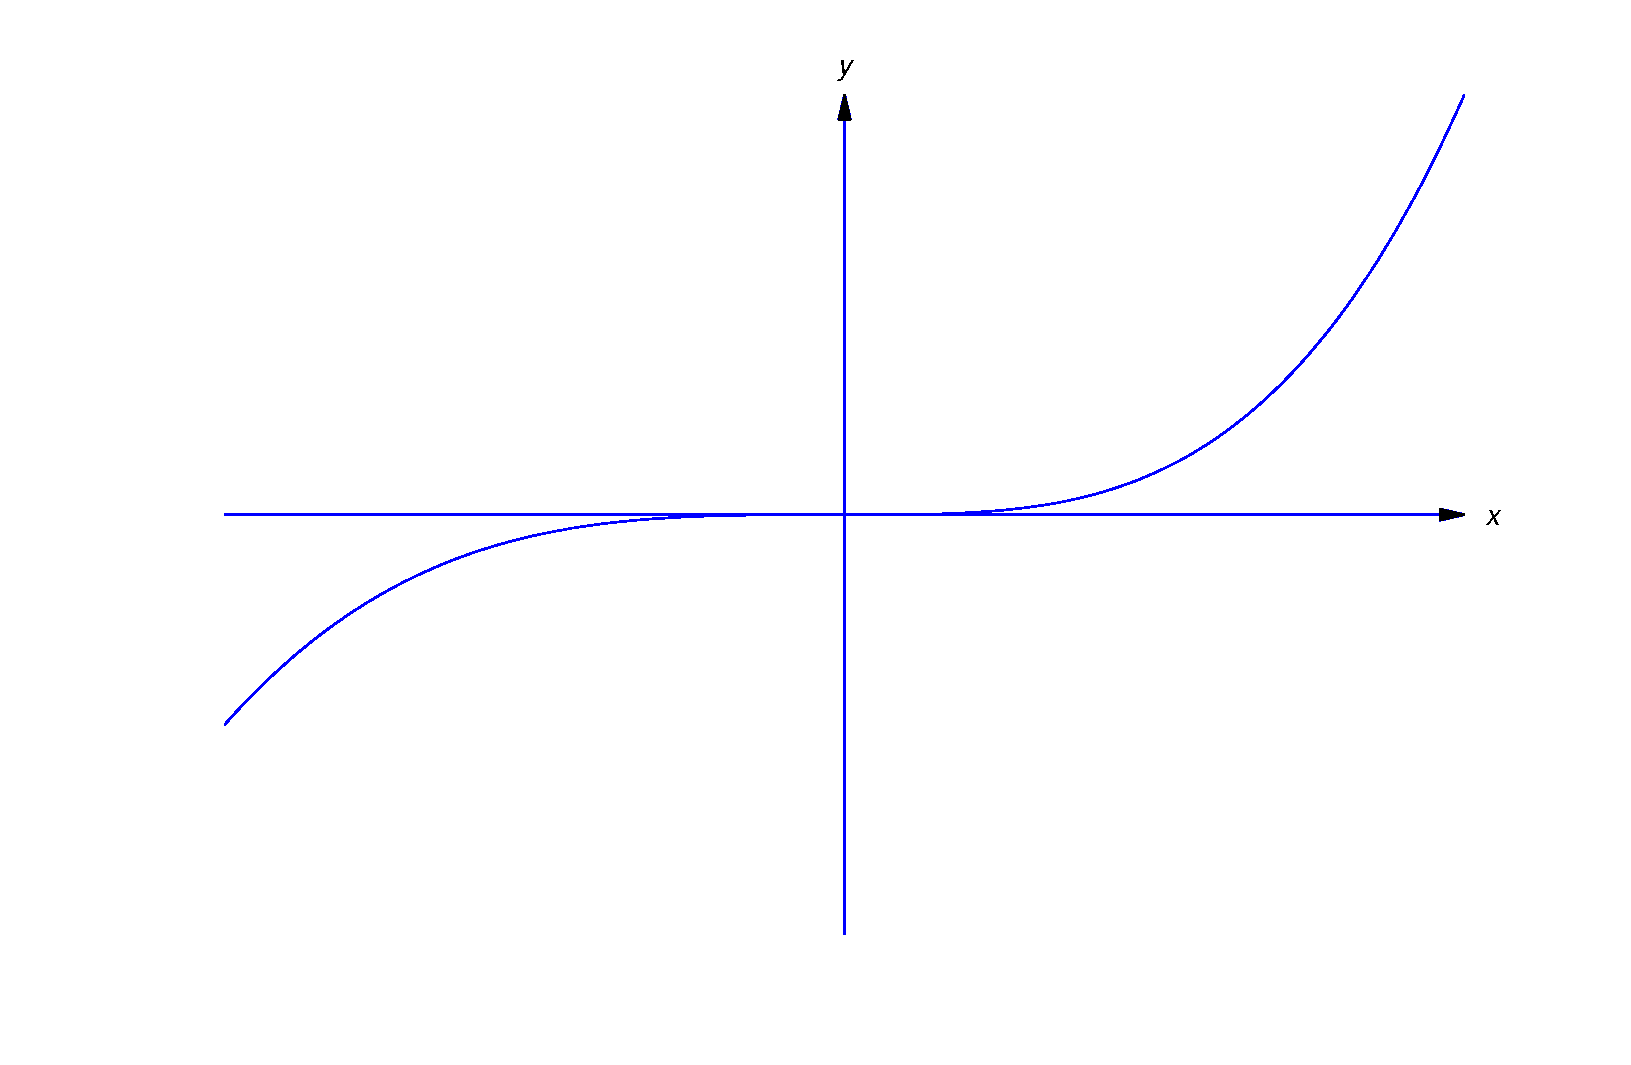
\includegraphics[bb=-78 148 689 643, width=5.67in, height=3.66in, keepaspectratio]{fig020302}
  \relax
  \caption{Two solutions ($y=0$ and $y=x^{10/3}$) of \eqref{eq:2.3.9} that differ on every interval containing $x_{0}=0$}
  \label{figure:2.3.2}
\end{figure}
\end{examplesolution}

\setcounter{example}{6}
\setcounter{equation}{11}
\begin{example}
  \label{example:2.3.7} \rm From Example~\ref{example:2.3.5}, the initial value problem
  \begin{equation}
    \label{eq:2.3.12}y'=\frac{10}{3}xy^{2/5},\quad y(0)=-1
  \end{equation}
  has a unique solution on some open interval that contains $x_{0}=0$. Find a solution and determine
  the largest open interval $(a,b)$ on which it's unique.
\end{example}
\setcounter{equation}{12}
\begin{examplesolution}
\solution Let $y$ be any solution of \eqref{eq:2.3.12}. Because of the initial condition $y(0)=-1$
and the continuity of $y$, there's an open interval $I$ that contains $x_{0}=0$ on which $y$ has no
zeros, and is consequently of the form \eqref{eq:2.3.11}. Setting $x=0$ and $y=-1$ in
\eqref{eq:2.3.11} yields $c=-1$, so
\begin{equation}
  \label{eq:2.3.13}y=(x^{2}-1)^{5/3}
\end{equation}
for $x$ in $I$. Therefore every solution of \eqref{eq:2.3.12} differs from zero and is given by
\eqref{eq:2.3.13} on $(-1,1)$; that is, \eqref{eq:2.3.13} is the unique solution of
\eqref{eq:2.3.12} on $(-1,1)$. This is the largest open interval on which \eqref{eq:2.3.12} has a
unique solution. To see this, note that \eqref{eq:2.3.13} is a solution of \eqref{eq:2.3.12} on
$(-\infty,\infty)$. From Exercise~2.3.~\hspace*{-3pt}2.3.15, there are infinitely many
other solutions of \eqref{eq:2.3.12} that differ from \eqref{eq:2.3.13} on every open interval
larger than $(-1,1)$. One such solution is
\[
  y=\left\{
  \begin{array}{cl}
    (x^{2}-1)^{5/3}, & -1\le x\le1, \\[6pt]
    0,               & |x|>1.
  \end{array}\right.
\]
(Figure 2.3.3).
\end{examplesolution}

\setcounter{example}{7}
\setcounter{equation}{13}
\begin{example}
  \label{example:2.3.8} \rm From Example~\ref{example:2.3.5}, the initial value problem
  \begin{equation}
    \label{eq:2.3.14}y'=\frac{10}{3}xy^{2/5},\quad y(0)=1
  \end{equation}
  has a unique solution on some open interval that contains $x_{0}=0$. Find the solution and
  determine the largest open interval on which it's unique.
\end{example}
\setcounter{equation}{14}
\begin{examplesolution}
\solution Let $y$ be any solution of \eqref{eq:2.3.14}. Because of the initial condition $y(0)=1$
and the continuity of $y$, there's an open interval $I$ that contains $x_{0}=0$ on which $y$ has no
zeros, and is consequently of the form \eqref{eq:2.3.11}. Setting $x=0$ and $y=1$ in
\eqref{eq:2.3.11} yields $c=1$, so
\begin{equation}
  \label{eq:2.3.15}y=(x^{2}+1)^{5/3}
\end{equation}
for $x$ in $I$. Therefore every solution of \eqref{eq:2.3.14} differs from zero and is given by
\eqref{eq:2.3.15} on $(-\infty,\infty)$; that is, \eqref{eq:2.3.15} is the unique solution of
\eqref{eq:2.3.14} on $(-\infty,\infty)$. Figure~2.3.4 shows the graph of this solution.
\end{examplesolution}

\section*{Section 2.4}
\setcounter{chapter}{2}
\setcounter{section}{4}

\setcounter{example}{0}
\setcounter{equation}{2}
\begin{example}
  \label{example:2.4.1} \rm Solve the Bernoulli equation
  \begin{equation}
    \label{eq:2.4.3}y'-y=xy^{2}.
  \end{equation}
\end{example}
\setcounter{figure}{0}
\begin{examplesolution}
\solution Since $y_{1}=e^{x}$ is a solution of $y'-y=0$, we look for solutions of \eqref{eq:2.4.3}
in the form $y=ue^{x}$, where
\[
  u'e^{x}=xu^{2}e^{2x}\mbox{\quad or, equivalently, \quad}u'=xu^{2}e^{x}.
\]
Separating variables yields
\[
  \frac{u'}{u^{2}}=xe^{x},
\]
and integrating yields
\[
  -\frac{1}{u}=(x-1)e^{x}+c.
\]
Hence,
\[
  u=-\frac{1}{(x-1)e^{x}+c}
\]
and
\[
  y=-\frac{1}{x-1+ce^{-x}}.
\]

Figure~\ref{figure:2.4.1} shows a direction field and some integral curves of \eqref{eq:2.4.3}.

\begin{figure}[H]
  \centering
  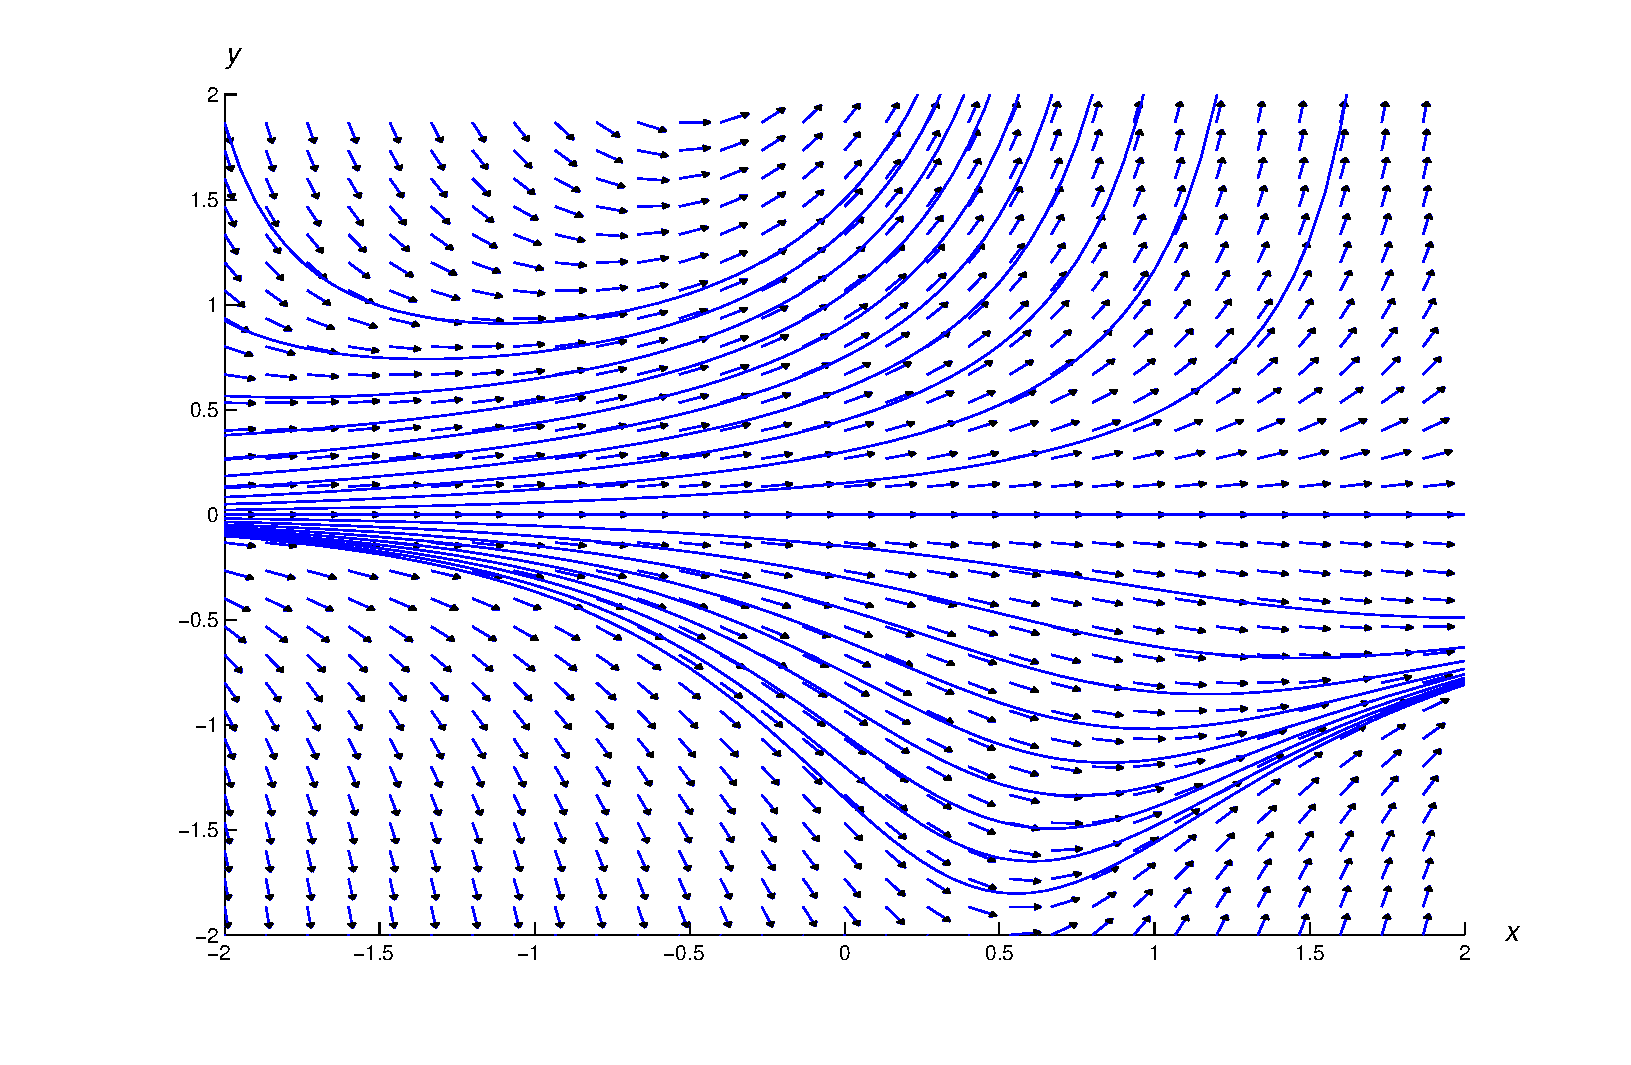
\includegraphics[bb=-78 148 689 643, width=5.67in, height=3.66in, keepaspectratio]{fig020401}
  \relax
  \caption{A direction field and integral curves for $y'-y=xy^{2}$}
  \label{figure:2.4.1}
\end{figure}
\end{examplesolution}

\setcounter{example}{1}
\setcounter{equation}{7}
\begin{example}
  \label{example:2.4.2}\rm Solve
  \begin{equation}
    \label{eq:2.4.8}y'=\frac{y+xe^{-y/x}}{x}.
  \end{equation}
\end{example}
\setcounter{figure}{1}
\begin{examplesolution}
\solution Substituting $y=ux$ into \eqref{eq:2.4.8} yields
\[
  u'x+u=\frac{ux+xe^{-ux/x}}{x}=u+e^{-u}.
\]
Simplifying and separating variables yields
\[
  e^{u}u'=\frac{1}{x}.
\]
Integrating yields $e^{u}=\ln|x|+c$. Therefore $u=\ln(\ln|x|+c)$ and $y=ux=x\ln(\ln|x|+c)$.

Figure~\ref{figure:2.4.2} shows a direction field and integral curves for \eqref{eq:2.4.8}.

\begin{figure}[H]
  \centering
  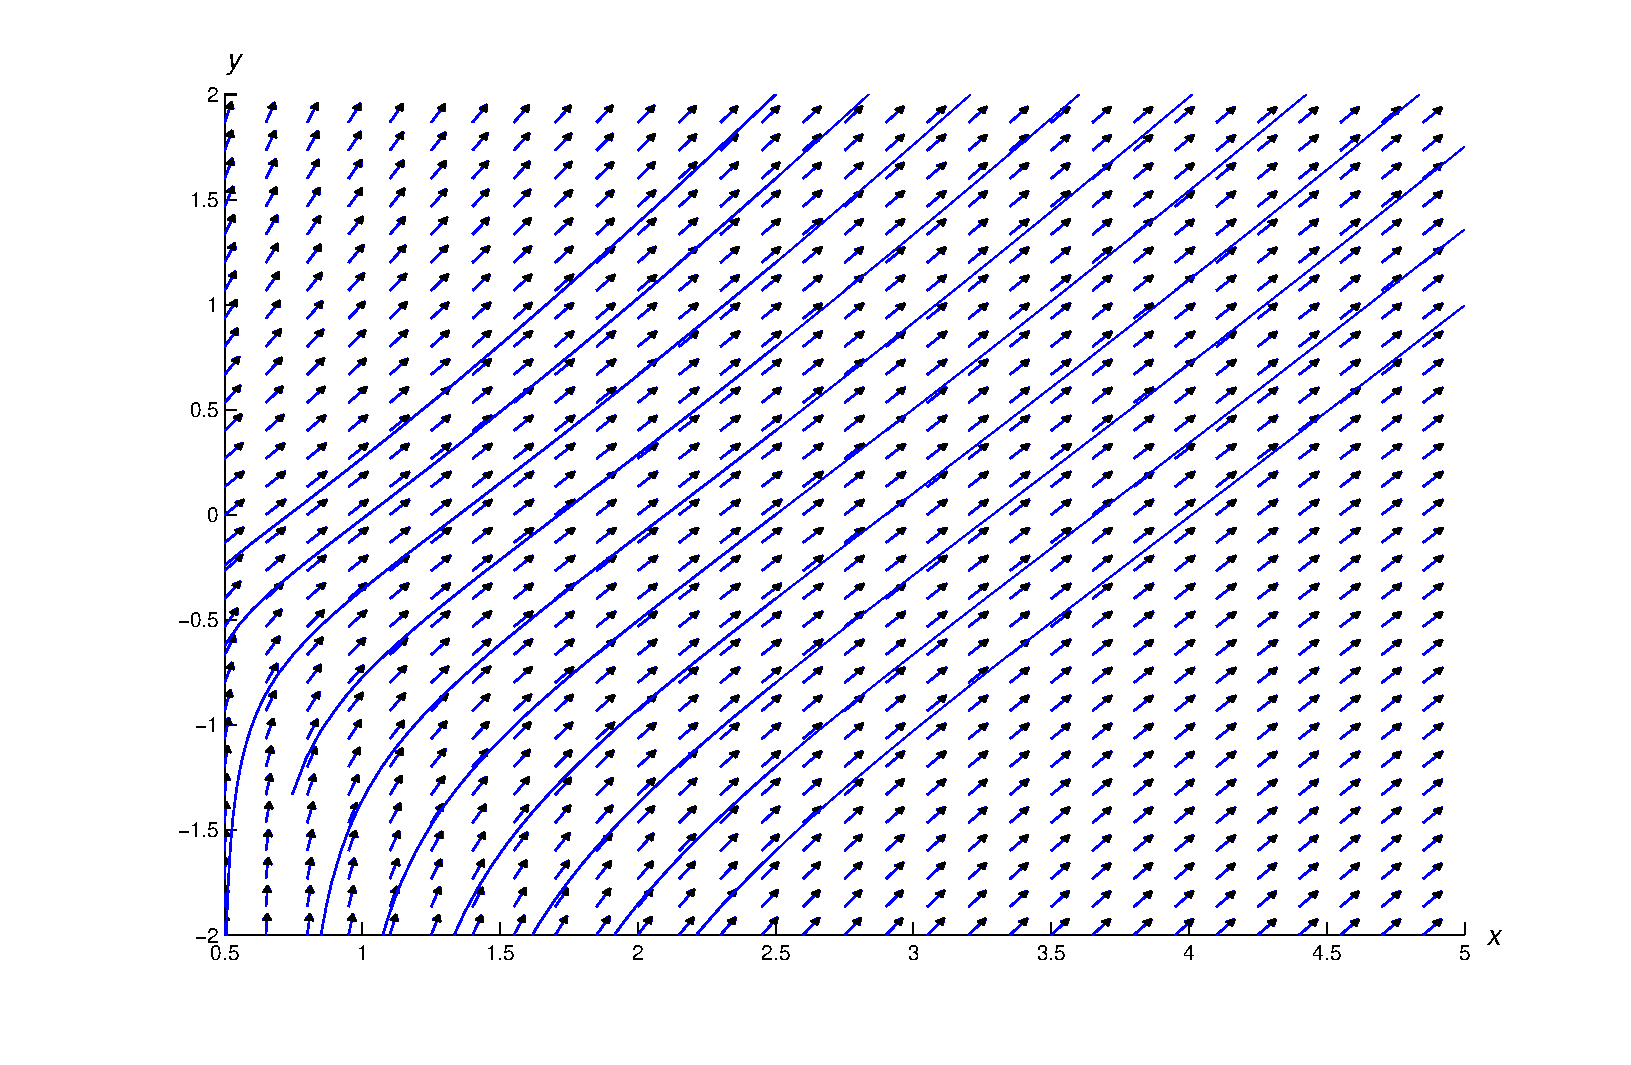
\includegraphics[bb=-78 148 689 643, width=5.67in, height=3.66in, keepaspectratio]{fig020402}
  \relax
  \caption{A direction field and some integral curves for $y'=\dst{\frac{y+xe^{-y/x}}{x}}$}
  \label{figure:2.4.2}
\end{figure}
\end{examplesolution}

\setcounter{example}{2}
\setcounter{equation}{8}
\begin{example}
  \label{example:2.4.3}\rm \mbox{}
  \newline
  \begin{alist}
    \item % (a)
    Solve
    \begin{equation}
      \label{eq:2.4.9}x^{2}y'=y^{2}+xy-x^{2}.
    \end{equation}

    \item % (b)
    Solve the initial value problem
    \begin{equation}
      \label{eq:2.4.10}x^{2}y'=y^{2}+xy-x^{2},\quad y(1)=2.
    \end{equation}
  \end{alist}
\end{example}
\setcounter{equation}{10}
\setcounter{figure}{2}
\begin{examplesolution}
\solutionpart{a} We first find solutions of \eqref{eq:2.4.9} on open intervals that don't contain
$x=0$. We can rewrite \eqref{eq:2.4.9} as
\[
  y'=\frac{y^{2}+xy-x^{2}}{x^{2}}
\]
for $x$ in any such interval. Substituting $y=ux$ yields
\[
  u'x+u=\frac{(ux)^{2}+x(ux)-x^{2}}{x^{2}}=u^{2}+u-1,
\]
so
\begin{equation}
  \label{eq:2.4.11}u'x=u^{2}-1.
\end{equation}
By inspection this equation has the constant solutions $u\equiv1$ and $u\equiv-1$. Therefore $y=x$
and $y=-x$ are solutions of \eqref{eq:2.4.9}. If $u$ is a solution of \eqref{eq:2.4.11} that doesn't
assume the values $\pm1$ on some interval, separating variables yields
\[
  \frac{u'}{u^{2}-1}=\frac{1}{x},
\]
or, after a partial fraction expansion,
\[
  \frac{1}{2}\left[\frac{1}{u-1}-\frac{1}{u+1}\right]u'= \frac{1}{x}.
\]
Multiplying by 2 and integrating yields
\[
  \ln\left|\frac{u-1}{u+1}\right|=2\ln|x|+k,
\]
or
\[
  \left|\frac{u-1}{u+1}\right|=e^{k}x^{2},
\]
which holds if
\begin{equation}
  \label{eq:2.4.12}\frac{u-1}{u+1}=cx^{2}
\end{equation}
where $c$ is an arbitrary constant. Solving for $u$ yields
\[
  u=\frac{1+cx^{2}}{1-cx^{2}}.
\]

\begin{figure}[H]
  \relax
  \begin{minipage}[b]{0.5\linewidth}
    \centering
    \scalebox{.6}{
    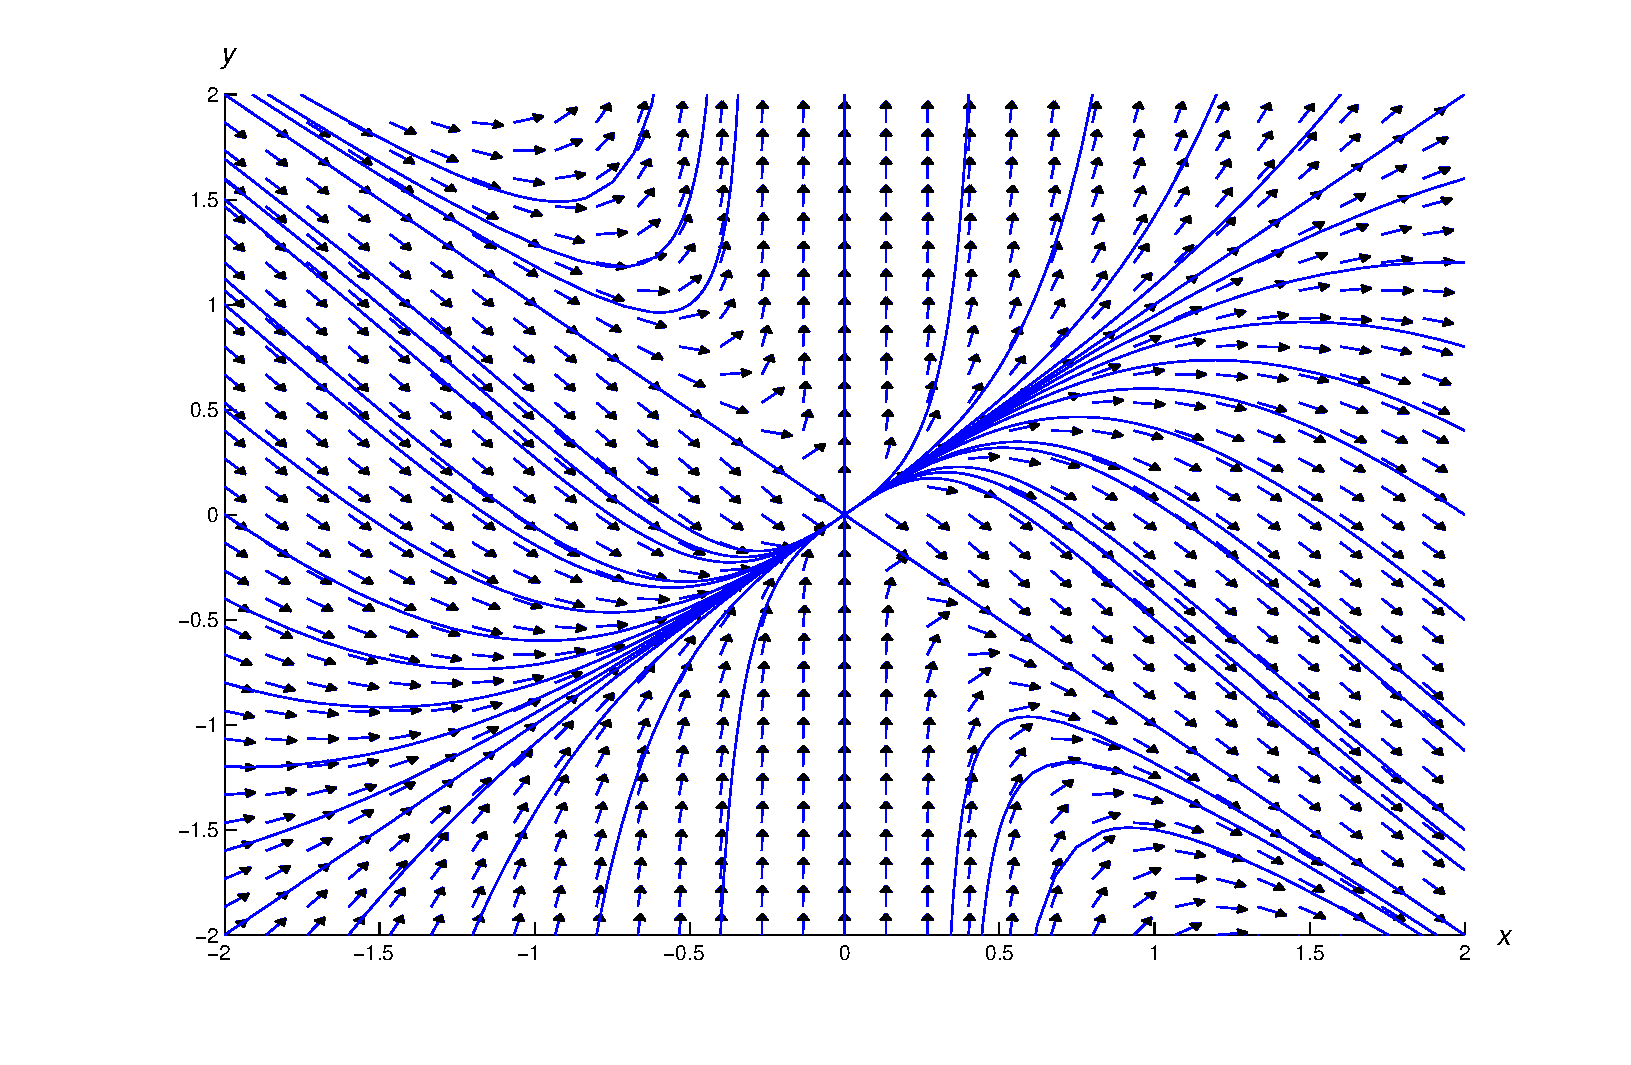
\includegraphics[bb=-78 148 689 643, width=5.67in, height=3.66in, keepaspectratio]{fig020403}
    }
    \relax
    \caption{A direction field and integral curves for $x^{2}y'=y^{2}+xy-x^{2}$}
    \label{figure:2.4.3}
  \end{minipage}
  \hspace{0.6cm}
  \begin{minipage}[b]{0.5\linewidth}
    \centering
    \scalebox{.7}{
    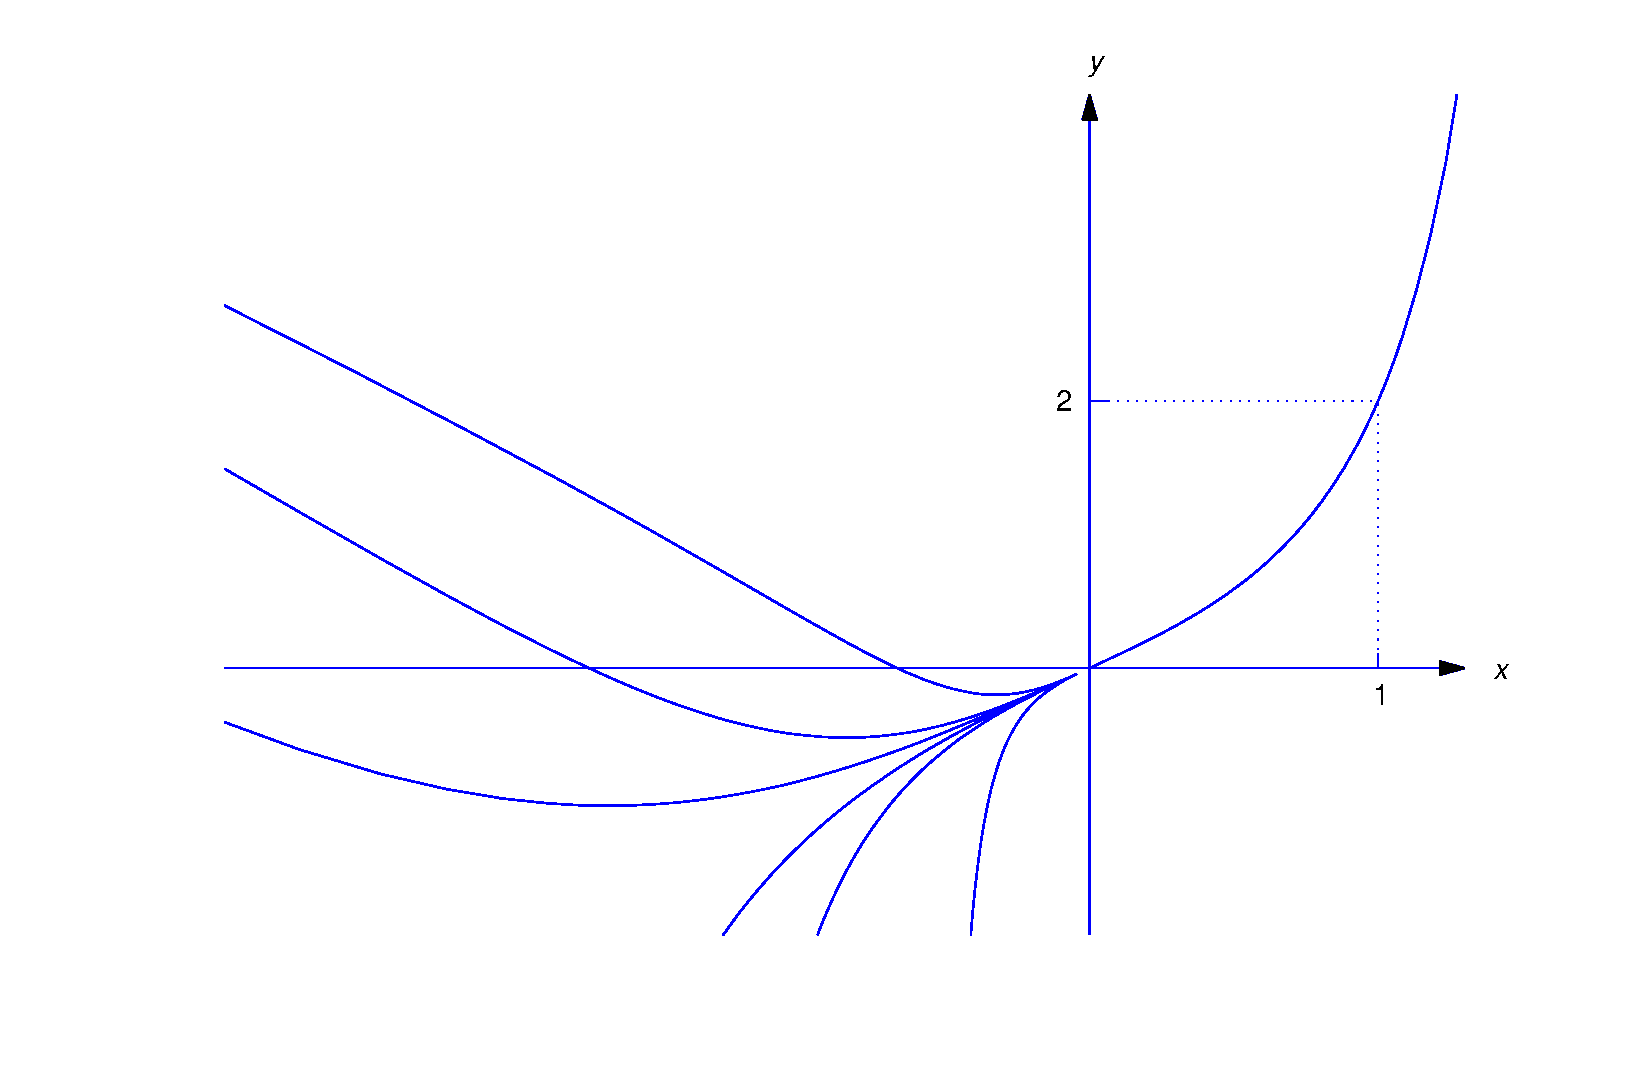
\includegraphics[bb=-78 148 689 643, width=5.67in, height=3.66in, keepaspectratio]{fig020404}}
    \caption{Solutions of $x^{2}y'=y^{2}+xy-x^{2}$,\; $y(1)=2$}
    \label{figure:2.4.4}
  \end{minipage}
\end{figure}

\noindent
Therefore
\begin{equation}
  \label{eq:2.4.13}y=ux=\frac{x(1+cx^{2})}{1-cx^{2}}
\end{equation}
is a solution of \eqref{eq:2.4.9} for any choice of the constant $c$. Setting $c=0$ in
\eqref{eq:2.4.13} yields the solution $y=x$. However, the solution $y=-x$ can't be obtained from
\eqref{eq:2.4.13}. Thus, the solutions of \eqref{eq:2.4.9} on intervals that don't contain $x=0$ are
$y=-x$ and functions of the form \eqref{eq:2.4.13}.

The situation is more complicated if $x=0$ is in the open interval. First, note that $y=-x$ satisfies
\eqref{eq:2.4.9} on $(-\infty,\infty)$. If $c_{1}$ and $c_{2}$ are arbitrary constants, the function
\begin{equation}
  \label{eq:2.4.14}y=\left\{
  \begin{array}{ll}
    \dst\frac{x(1+c_{1}x^{2})}{1-c_{1}x^{2}},        & a<x<0,    \\
    [2\jot]\dst\frac{x(1+c_{2}x^{2})}{1-c_{2}x^{2}}, & 0\le x<b,
  \end{array}\right.
\end{equation}
is a solution of \eqref{eq:2.4.9} on $(a,b)$, where
\[
  a=\left\{
  \begin{array}{cl}
    -\dst\frac{1}{\sqrt{c_{1}}} & \mbox{ if }c_{1}>0,   \\
    -\infty                     & \mbox{ if }c_{1}\le0,
  \end{array}\right.\mbox{\quad and \quad}b=\left\{
  \begin{array}{cl}
    \dst\frac{1}{\sqrt{c_{2}}} & \mbox{ if }c_{2}>0,   \\
    \infty                     & \mbox{ if }c_{2}\le0.
  \end{array}\right.
\]
We leave it to you to verify this. To do so, note that if $y$ is any function of the form
\eqref{eq:2.4.13} then $y(0)=0$ and $y'(0)=1$.

Figure~\ref{figure:2.4.3} shows a direction field and some integral curves for \eqref{eq:2.4.9}.

\solutionpart{b} We could obtain $c$ by imposing the initial condition $y(1)=2$ in
\eqref{eq:2.4.13}, and then solving for $c$. However, it's easier to use \eqref{eq:2.4.12}. Since
$u=y/x$, the initial condition $y(1)=2$ implies that $u(1)=2$. Substituting this into
\eqref{eq:2.4.12} yields $c=1/3$. Hence, the solution of \eqref{eq:2.4.10} is
\[
  y=\frac{x(1+x^{2}/3)}{1-x^{2}/3}.
\]
The interval of validity of this solution is $(-\sqrt{3},\sqrt{3})$. However, the largest interval
on which \eqref{eq:2.4.10} has a unique solution is $(0,\sqrt{3})$. To see this, note from
\eqref{eq:2.4.14} that any function of the form
\begin{equation}
  \label{eq:2.4.15}y=\left\{
  \begin{array}{ll}
    \dst\frac{x(1+cx^{2})}{1-cx^{2}},   & a<x\le0,         \\[2\jot]
    \dst\frac{x(1+x^{2}/3)}{1-x^{2}/3}, & 0\le x<\sqrt{3},
  \end{array}\right.
\end{equation}
is a solution of \eqref{eq:2.4.10} on $(a,\sqrt{3})$, where $a=-1/\sqrt{c}$ if $c>0$ or $a=-\infty$
if $c\le0$. (Why doesn't this contradict Theorem~2.3.1?)

Figure~\ref{figure:2.4.4} shows several solutions of the initial value problem~\eqref{eq:2.4.10}.
Note that these solutions coincide on $(0,\sqrt{3})$.
\end{examplesolution}

\section*{Section 2.5}
\setcounter{chapter}{2}
\setcounter{section}{5}

\setcounter{example}{0}
\setcounter{equation}{3}
\begin{example}
  \label{example:2.5.1} \rm Show that
  \begin{equation}
    \label{eq:2.5.4}x^{4}y^{3}+x^{2}y^{5}+2xy=c
  \end{equation}
  is an implicit solution of
  \begin{equation}
    \label{eq:2.5.5}(4x^{3}y^{3}+2xy^{5}+2y)\,dx+(3x^{4}y^{2}+5x^{2}y^{4}+2x)\,dy=0.
  \end{equation}
\end{example}
\begin{examplesolution}
\solution Regarding $y$ as a function of $x$ and differentiating \eqref{eq:2.5.4} implicitly with
respect to $x$ yields
\[
  (4x^{3}y^{3}+2xy^{5}+2y)+(3x^{4}y^{2}+5x^{2}y^{4}+2x)\,\frac{dy}{dx}=0.
\]
Similarly, regarding $x$ as a function of $y$ and differentiating \eqref{eq:2.5.4} implicitly with
respect to $y$ yields
\[
  (4x^{3}y^{3}+2xy^{5}+2y)\frac{dx}{dy}+(3x^{4}y^{2}+5x^{2}y^{4}+2x)=0.
\]
Therefore \eqref{eq:2.5.4} is an implicit solution of \eqref{eq:2.5.5} in either of its two possible
interpretations. \bbox
\end{examplesolution}

\setcounter{example}{1}
\begin{example}
  \label{example:2.5.2} \rm Show that the equation
  \[
    3x^{2}y\,dx+4x^{3}\,dy=0
  \]
  is not exact on any open rectangle.
\end{example}
\begin{examplesolution}
\solution Here
\[
  M(x,y)=3x^{2}y\mbox{\quad and \quad}N(x,y)=4x^{3}
\]
so
\[
  M_{y}(x,y)=3x^{2}\mbox{\quad and \quad}N_{x}(x,y)=12x^{2}.
\]
Therefore $M_{y}=N_{x}$ on the line $x=0$, but not on any open rectangle, so there's no function $F$
such that $F_{x}(x,y)=M(x,y)$ and $F_{y}(x,y)=N(x,y)$ for all $(x,y)$ on any open rectangle. \bbox
\end{examplesolution}

\setcounter{example}{2}
\setcounter{equation}{12}
\begin{example}
  \label{example:2.5.3} \rm Solve
  \begin{equation}
    \label{eq:2.5.13}(4x^{3}y^{3}+3x^{2})\,dx+(3x^{4}y^{2}+6y^{2})\,dy=0.
  \end{equation}
\end{example}
\setcounter{equation}{13}
\setcounter{figure}{0}
\begin{examplesolution}
\solution{(Method 1)} Here
\[
  M(x,y)=4x^{3}y^{3}+3x^{2},\quad N(x,y)=3x^{4}y^{2}+6y^{2},
\]
and
\[
  M_{y}(x,y)=N_{x}(x,y)=12x^{3}y^{2}
\]
for all $(x,y)$. Therefore Theorem~2.5.2 implies that there's a function $F$ such that
\begin{equation}
  \label{eq:2.5.14}F_{x}(x,y)=M(x,y)=4x^{3}y^{3}+3x^{2}
\end{equation}
and
\begin{equation}
  \label{eq:2.5.15}F_{y}(x,y)=N(x,y)=3x^{4}y^{2}+6y^{2}
\end{equation}
for all $(x,y)$. To find $F$, we integrate \eqref{eq:2.5.14} with respect to $x$ to obtain
\begin{equation}
  \label{eq:2.5.16}F(x,y)=x^{4}y^{3}+x^{3}+\phi(y),
\end{equation}
where $\phi(y)$ is the ``constant'' of integration. (Here $\phi$ is ``constant'' in that it's
independent of $x$, the variable of integration.) If $\phi$ is any differentiable function of $y$
then $F$ satisfies \eqref{eq:2.5.14}. To determine $\phi$ so that $F$ also satisfies
\eqref{eq:2.5.15}, assume that $\phi$ is differentiable and differentiate $F$ with respect to $y$.
This yields
\[
  F_{y}(x,y)=3x^{4}y^{2}+\phi'(y).
\]
Comparing this with \eqref{eq:2.5.15} shows that
\[
  \phi'(y)=6y^{2}.
\]
We integrate this with respect to $y$ and take the constant of integration to be zero because we're
interested only in finding {\relax\it some} $F$ that satisfies \eqref{eq:2.5.14} and
\eqref{eq:2.5.15}. This yields
\[
  \phi(y)=2y^{3}.
\]
Substituting this into \eqref{eq:2.5.16} yields
\begin{equation}
  \label{eq:2.5.17}F(x,y)=x^{4}y^{3}+x^{3}+2y^{3}.
\end{equation}
Now Theorem~2.5.1 implies that
\[
  x^{4}y^{3}+x^{3}+2y^{3}=c
\]
is an implicit solution of \eqref{eq:2.5.13}. Solving this for $y$ yields the explicit solution
\[
  y=\left(\frac{c-x^{3}}{2+x^{4}}\right)^{1/3}.
\]

\solution{(Method 2)} Instead of first integrating \eqref{eq:2.5.14} with respect to $x$, we could
begin by integrating \eqref{eq:2.5.15} with respect to $y$ to obtain
\begin{equation}
  \label{eq:2.5.18}F(x,y)=x^{4}y^{3}+2y^{3}+\psi(x),
\end{equation}
where $\psi$ is an arbitrary function of $x$. To determine $\psi$, we assume that $\psi$ is
differentiable and differentiate $F$ with respect to $x$, which yields
\[
  F_{x}(x,y)=4x^{3}y^{3}+\psi'(x).
\]
Comparing this with \eqref{eq:2.5.14} shows that
\[
  \psi'(x)=3x^{2}.
\]
Integrating this and again taking the constant of integration to be zero yields
\[
  \psi(x)=x^{3}.
\]
Substituting this into \eqref{eq:2.5.18} yields \eqref{eq:2.5.17}.

Figure~\ref{figure:2.5.1} shows a direction field and some integral curves of \eqref{eq:2.5.13}.

\begin{figure}[H]
  \centering
  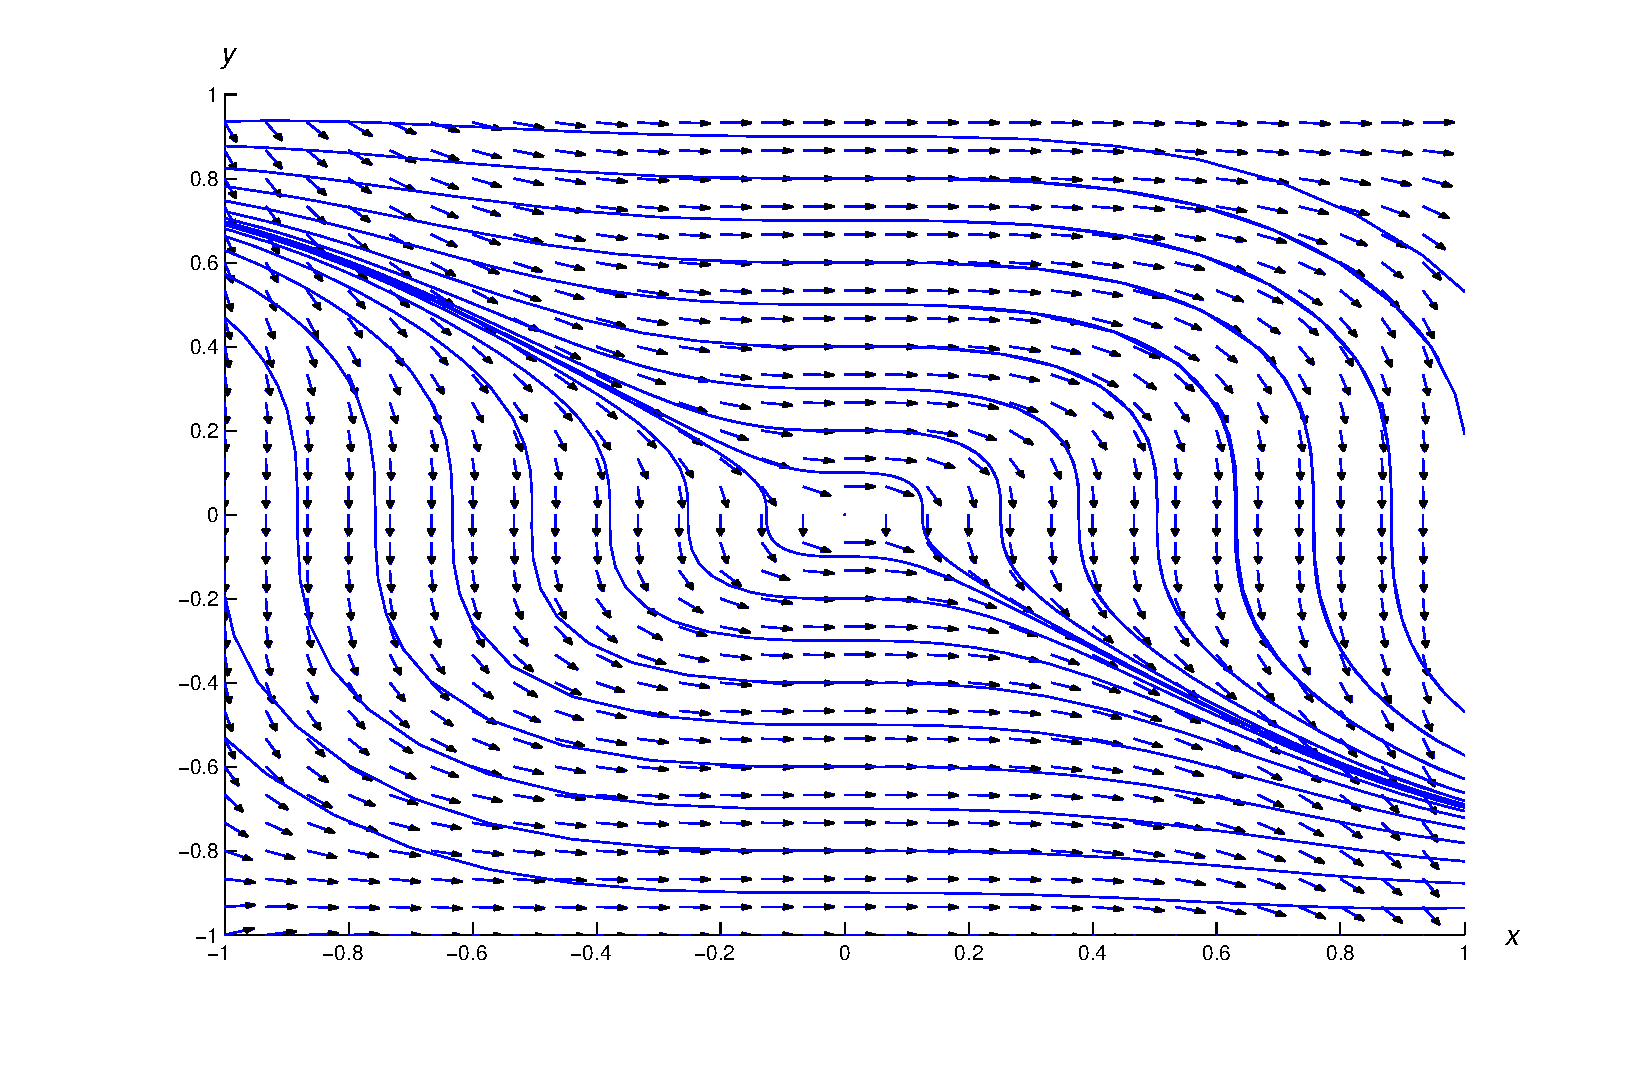
\includegraphics[bb=-78 148 689 643, width=5.67in, height=3.66in, keepaspectratio]{fig020501}
  \relax
  \caption{A direction field and integral curves for $(4x^{3}y^{3}+3x^{2})\,dx+(3x^{4}y^{2}+6y^{2})\,dy=0$}
  \label{figure:2.5.1}
\end{figure}
\end{examplesolution}

\setcounter{example}{3}
\setcounter{equation}{20}
\begin{example}
  \label{example:2.5.4} \rm Solve the equation
  \begin{equation}
    \label{eq:2.5.21}(ye^{xy}\tan x+e^{xy}\sec^{2}x)\,dx+xe^{xy}\tan x\,dy=0.
  \end{equation}
\end{example}
\setcounter{equation}{21}
\begin{examplesolution}
\solution We leave it to you to check that $M_{y}=N_{x}$ on any open rectangle where $\tan x$ and
$\sec x$ are defined. Here we must find a function $F$ such that
\begin{equation}
  \label{eq:2.5.22}F_{x}(x,y)=ye^{xy}\tan x+e^{xy}\sec^{2}x
\end{equation}
and
\begin{equation}
  \label{eq:2.5.23}F_{y}(x,y)=xe^{xy}\tan x.
\end{equation}
It's difficult to integrate \eqref{eq:2.5.22} with respect to $x$, but easy to integrate
\eqref{eq:2.5.23} with respect to $y$. This yields
\begin{equation}
  \label{eq:2.5.24}F(x,y)=e^{xy}\tan x+\psi(x).
\end{equation}
Differentiating this with respect to $x$ yields
\[
  F_{x}(x,y)=ye^{xy}\tan x+e^{xy}\sec^{2}x+\psi'(x).
\]
Comparing this with \eqref{eq:2.5.22} shows that $\psi'(x)=0$. Hence, $\psi$ is a constant, which we
can take to be zero in \eqref{eq:2.5.24}, and
\[
  e^{xy}\tan x=c
\]
is an implicit solution of \eqref{eq:2.5.21}. \bbox
\end{examplesolution}

\setcounter{example}{4}
\setcounter{equation}{24}
\begin{example}
  \label{example:2.5.5} \rm Verify that the equation
  \begin{equation}
    \label{eq:2.5.25}3x^{2}y^{2}\,dx+6x^{3}y\,dy=0
  \end{equation}
  is not exact, and show that the procedure for solving exact equations fails when applied to
  \eqref{eq:2.5.25}.
\end{example}
\setcounter{equation}{25}
\begin{examplesolution}
\solution Here
\[
  M_{y}(x,y)=6x^{2}y\mbox{\quad and \quad }N_{x}(x,y)=18x^{2}y,
\]
so \eqref{eq:2.5.25} isn't exact. Nevertheless, let's try to find a function $F$ such that
\begin{equation}
  \label{eq:2.5.26}F_{x}(x,y)=3x^{2}y^{2}
\end{equation}
and
\begin{equation}
  \label{eq:2.5.27}F_{y}(x,y)=6x^{3}y.
\end{equation}
Integrating \eqref{eq:2.5.26} with respect to $x$ yields
\[
  F(x,y)=x^{3}y^{2}+\phi(y),
\]
and differentiating this with respect to $y$ yields
\[
  F_{y}(x,y)=2x^{3}y+\phi'(y).
\]
For this equation to be consistent with \eqref{eq:2.5.27},
\[
  6x^{3}y=2x^{3}y+\phi'(y),
\]
or
\[
  \phi'(y)=4x^{3}y.
\]
This is a contradiction, since $\phi'$ must be independent of $x$. Therefore the procedure fails.
\end{examplesolution}

\section*{Section 2.6}
\setcounter{chapter}{2}
\setcounter{section}{6}

\setcounter{example}{0}
\setcounter{equation}{12}
\begin{example}
  \label{example:2.6.1} \rm Find an integrating factor for the equation
  \begin{equation}
    \label{eq:2.6.13}(2xy^{3}-2x^{3}y^{3}-4xy^{2}+2x)\,dx+(3x^{2}y^{2}+4y)\,dy=0
  \end{equation}
  and solve the equation.
\end{example}
\setcounter{equation}{13}
\setcounter{figure}{0}
\begin{examplesolution}
\solution In \eqref{eq:2.6.13}
\[
  M=2xy^{3}-2x^{3}y^{3}-4xy^{2}+2x,\ N=3x^{2}y^{2}+4y,
\]
and
\[
  M_{y}-N_{x}=(6xy^{2}-6x^{3}y^{2}-8xy)-6xy^{2}=-6x^{3}y^{2}-8xy,
\]
so \eqref{eq:2.6.13} isn't exact. However,
\[
  \frac{M_{y}-N_{x}}{N}=-\frac{6x^{3}y^{2}+8xy}{3x^{2}y^{2}+4y}=-2x
\]
is independent of $y$, so Theorem~2.6.1\part{a} applies with $p(x)=-2x$. Since
\[
  \int p(x)\,dx=-\int2x\,dx=-x^{2},
\]
$\mu(x)=e^{-x^{2}}$ is an integrating factor. Multiplying \eqref{eq:2.6.13} by $\mu$ yields the
exact equation
\begin{equation}
  \label{eq:2.6.14}e^{-x^{2}}(2xy^{3}-2x^{3}y^{3}-4xy^{2}+2x)\,dx+ e^{-x^{2}}(3x^{2}y^{2}+4y)\,dy=0.
\end{equation}

To solve this equation, we must find a function $F$ such that
\begin{equation}
  \label{eq:2.6.15}F_{x}(x,y)=e^{-x^{2}}(2xy^{3}-2x^{3}y^{3}-4xy^{2}+2x)
\end{equation}
and
\begin{equation}
  \label{eq:2.6.16}F_{y}(x,y)=e^{-x^{2}}(3x^{2}y^{2}+4y).
\end{equation}
Integrating \eqref{eq:2.6.16} with respect to $y$ yields
\begin{equation}
  \label{eq:2.6.17}F(x,y)=e^{-x^{2}}(x^{2}y^{3}+2y^{2})+\psi(x).
\end{equation}
Differentiating this with respect to $x$ yields
\[
  F_{x}(x,y)=e^{-x^{2}}(2xy^{3}-2x^{3}y^{3}-4xy^{2})+\psi'(x).
\]
Comparing this with \eqref{eq:2.6.15} shows that $\psi'(x)= 2xe^{-x^{2}}$; therefore, we can let
$\psi(x)=-e^{-x^{2}}$ in \eqref{eq:2.6.17} and conclude that
\[
  e^{-x^{2}}\left(y^{2}(x^{2}y+2)-1\right)=c
\]
is an implicit solution of \eqref{eq:2.6.14}. It is also an implicit solution of \eqref{eq:2.6.13}.

Figure~\ref{figure:2.6.1} shows a direction field and some integral curves for \eqref{eq:2.6.13}. \begin{figure}[H]
  \centering
  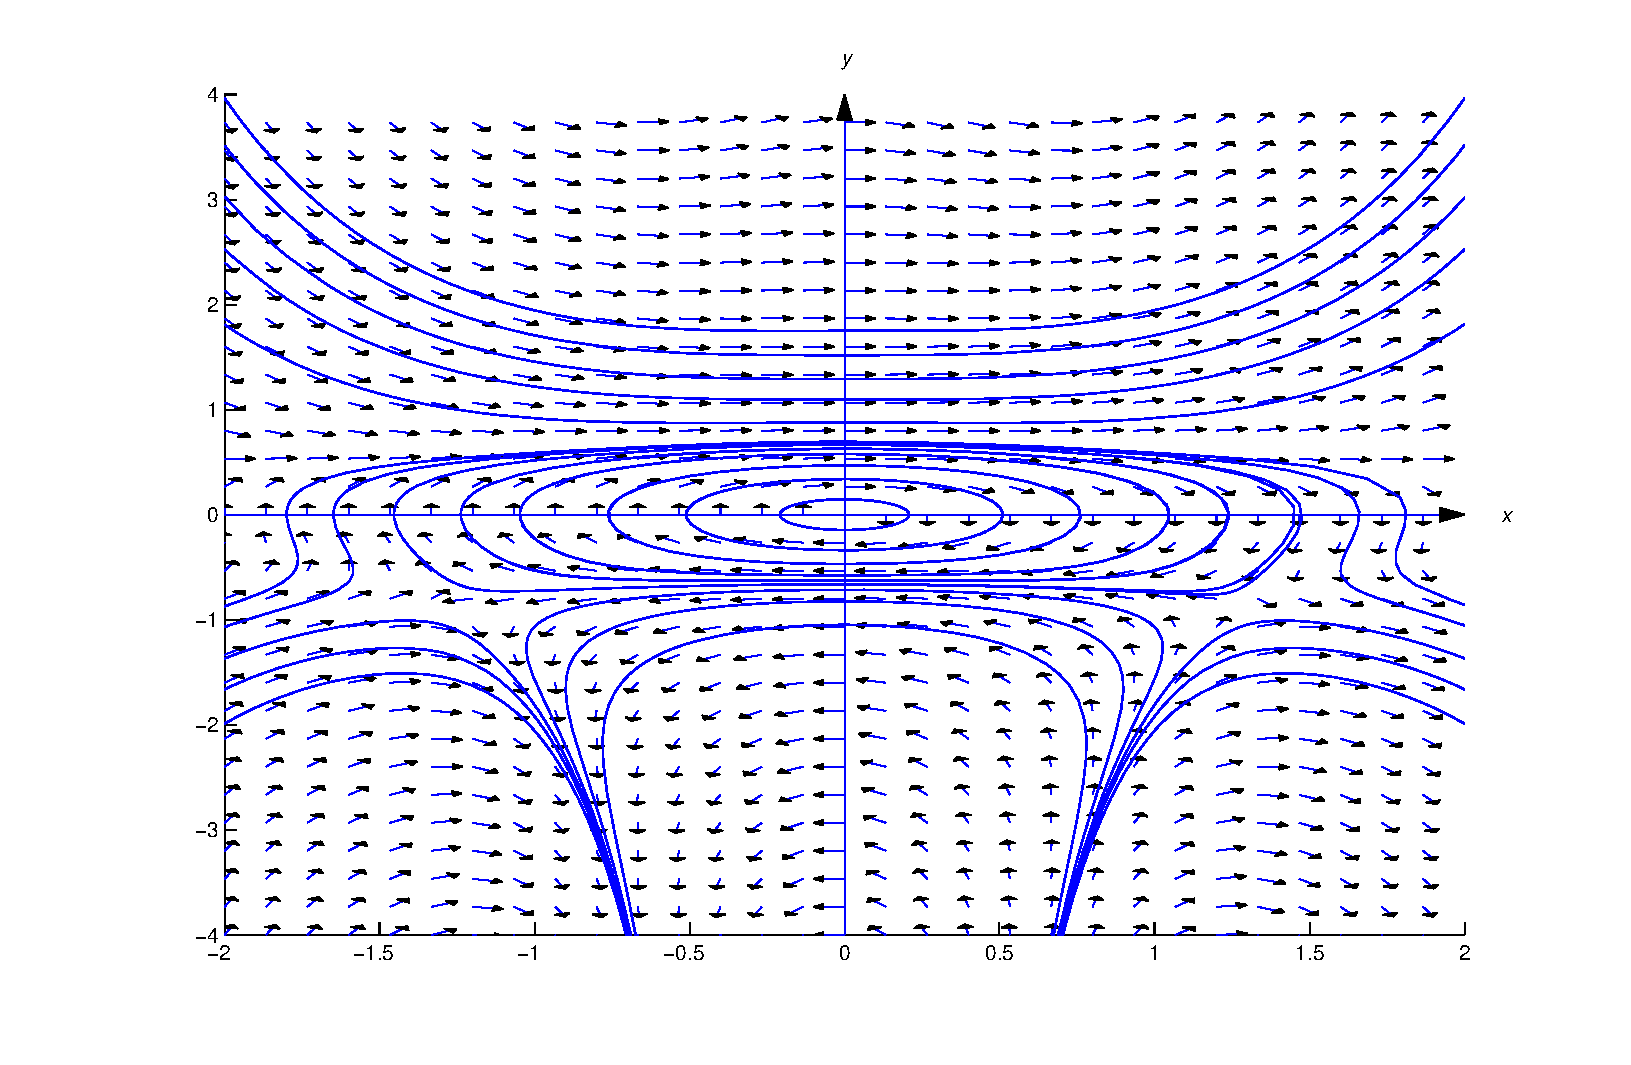
\includegraphics[bb=-78 148 689 643, width=5.67in, height=3.66in, keepaspectratio]{fig020601}
  \relax
  \caption{A direction field and integral curves for $(2xy^{3}-2x^{3}y^{3}-4xy^{2}+2x)\,dx+(3x^{2}y^{2}+4y)\,dy=0$}
  \label{figure:2.6.1}
\end{figure}
\end{examplesolution}

\setcounter{example}{1}
\setcounter{equation}{17}
\begin{example}
  \label{example:2.6.2} \rm Find an integrating factor for
  \begin{equation}
    \label{eq:2.6.18}2xy^{3}\,dx+(3x^{2}y^{2}+x^{2}y^{3}+1)\,dy=0
  \end{equation}
  and solve the equation.
\end{example}
\setcounter{equation}{18}
\setcounter{figure}{1}
\begin{examplesolution}
\solution In \eqref{eq:2.6.18},
\[
  M=2xy^{3},\quad N=3x^{2}y^{2}+x^{2}y^{3}+1,
\]
and
\[
  M_{y}-N_{x}=6xy^{2}-(6xy^{2}+2xy^{3})=-2xy^{3},
\]
so \eqref{eq:2.6.18} isn't exact. Moreover,
\[
  \frac{M_{y}-N_{x}}{N}=-\frac{2xy^{3}}{3x^{2}y^{2}+x^{2}y^{3}+1}
\]
is not independent of $y$, so Theorem~2.6.1(a) does not apply. However,
Theorem~2.6.1(b) does apply, since
\[
  \frac{N_{x}-M_{y}}{M}=\frac{2xy^{3}}{2xy^{3}}=1
\]
is independent of $x$, so we can take $q(y)=1$. Since
\[
  \int q(y)\,dy=\int\,dy=y,
\]
$\mu(y)=e^{y}$ is an integrating factor. Multiplying \eqref{eq:2.6.18} by $\mu$ yields the exact
equation
\begin{equation}
  \label{eq:2.6.19}2xy^{3}e^{y}\,dx+(3x^{2}y^{2}+x^{2}y^{3}+1)e^{y}\,dy=0.
\end{equation}
To solve this equation, we must find a function $F$ such that
\begin{equation}
  \label{eq:2.6.20}F_{x}(x,y)=2xy^{3}e^{y}
\end{equation}
and
\begin{equation}
  \label{eq:2.6.21}F_{y}(x,y)=(3x^{2}y^{2}+x^{2}y^{3}+1)e^{y}.
\end{equation}
Integrating \eqref{eq:2.6.20} with respect to $x$ yields
\begin{equation}
  \label{eq:2.6.22}F(x,y)=x^{2}y^{3}e^{y}+\phi(y).
\end{equation}
Differentiating this with respect to $y$ yields
\[
  F_{y}=(3x^{2}y^{2}+x^{2}y^{3})e^{y}+\phi'(y),
\]
and comparing this with \eqref{eq:2.6.21} shows that $\phi'(y)=e^{y}$. Therefore we set
$\phi(y)=e^{y}$ in \eqref{eq:2.6.22} and conclude that
\[
  (x^{2}y^{3}+1)e^{y}=c
\]
is an implicit solution of \eqref{eq:2.6.19}. It is also an implicit solution of \eqref{eq:2.6.18}.
Figure~\ref{figure:2.6.2} shows a direction field and some integral curves for
\eqref{eq:2.6.18}.\bbox

\begin{figure}[H]
  \centering
  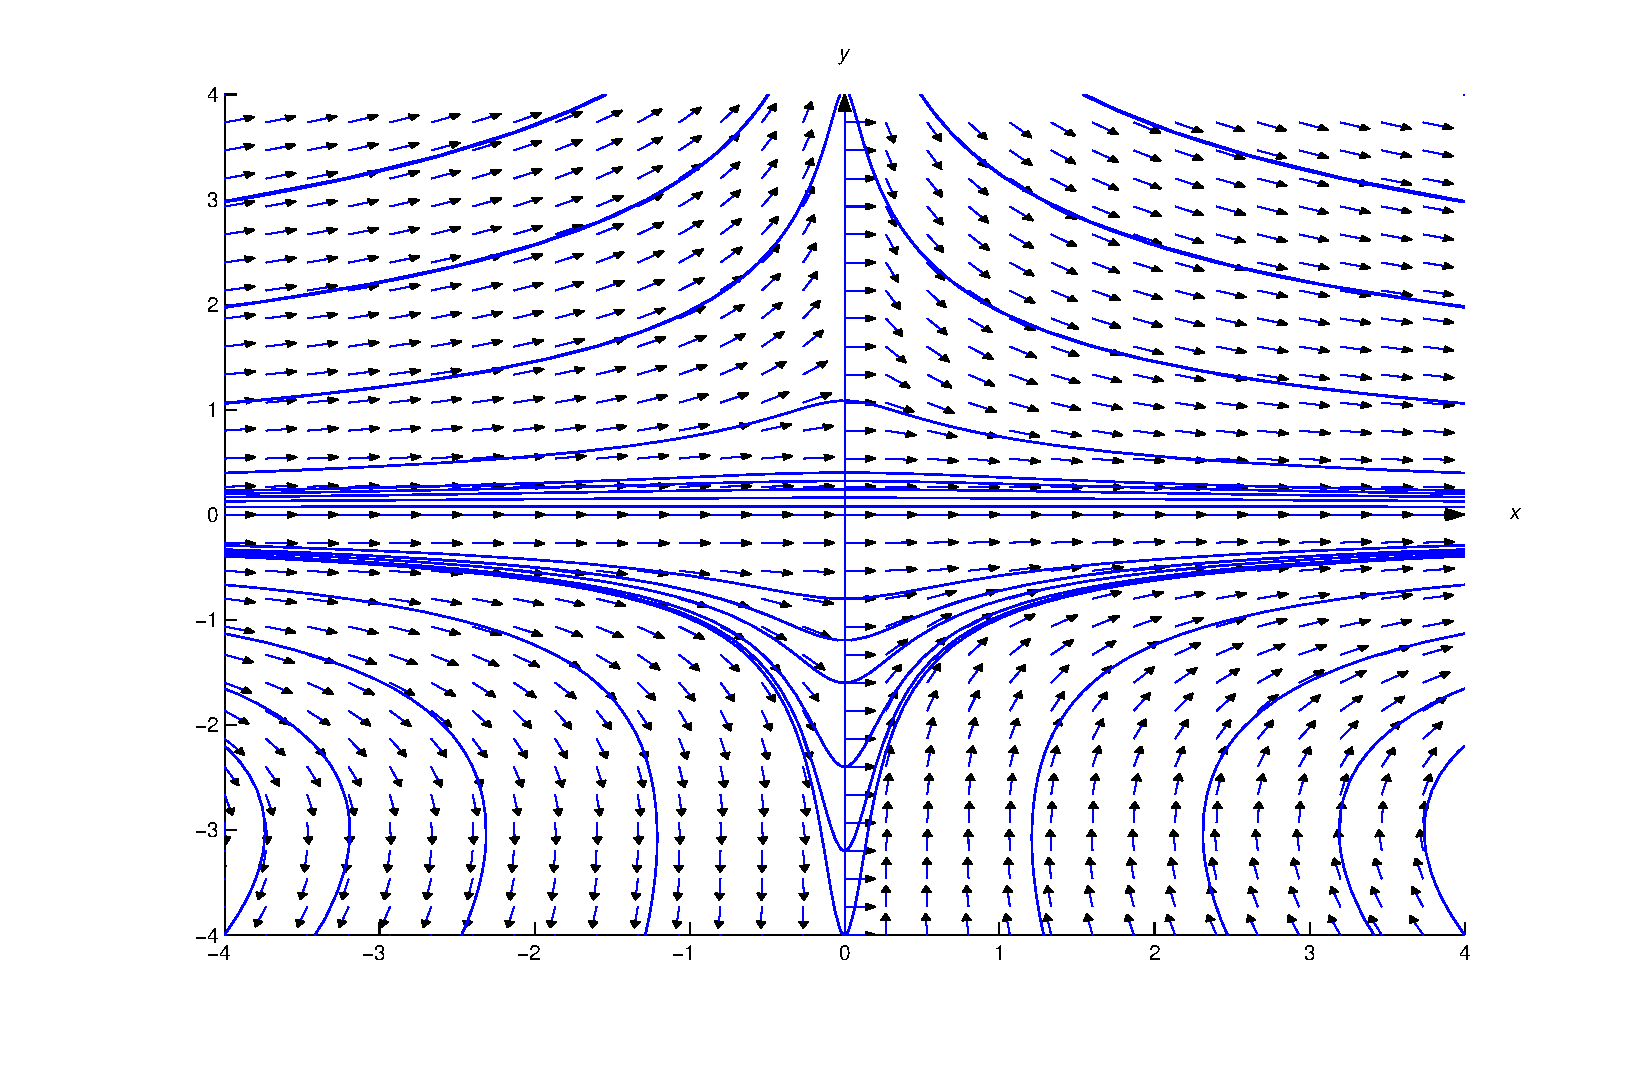
\includegraphics[bb=-78 148 689 643, width=5.67in, height=3.66in, keepaspectratio]{fig020602}
  \relax
  \caption{A direction field and integral curves for $2xy^{3}e^{y}\,dx+(3x^{2}y^{2}+x^{2}y^{3}+1)e^{y}\,dy=0$}
  \label{figure:2.6.2}
\end{figure}
\end{examplesolution}

\setcounter{example}{2}
\setcounter{equation}{22}
\begin{example}
  \label{example:2.6.3} \rm Find an integrating factor for
  \begin{equation}
    \label{eq:2.6.23}(3xy+6y^{2})\,dx+(2x^{2}+9xy)\,dy=0
  \end{equation}
  and solve the equation.
\end{example}
\setcounter{equation}{23}
\begin{examplesolution}
\solution In \eqref{eq:2.6.23}
\[
  M=3xy+6y^{2},\ N=2x^{2}+9xy,
\]
and
\[
  M_{y}-N_{x}=(3x+12y)-(4x+9y)=-x+3y.
\]
Therefore
\[
  \frac{M_{y}-N_{x}}{M}=\frac{-x+3y}{3xy+6y^{2}}\mbox{\quad and \quad}{\frac{N_{x}-M_{y}}{N}}=\frac{x-3y}{2x^{2}+9xy},
\]
so Theorem~2.6.1 does not apply. Following the more general argument that led to
Theorem~2.6.1, we look for functions $p=p(x)$ and $q=q(y)$ such that
\[
  M_{y}-N_{x}=p(x)N-q(y)M;
\]
that is,
\[
  -x+3y=p(x)(2x^{2}+9xy)-q(y)(3xy+6y^{2}).
\]
Since the left side contains only first degree terms in $x$ and $y$, we rewrite this equation as
\[
  xp(x)(2x+9y)-yq(y)(3x+6y)=-x+3y.
\]
This will be an identity if
\begin{equation}
  \label{eq:2.6.24}xp(x)=A\mbox{\quad and\quad}yq(y)=B,
\end{equation}
where $A$ and $B$ are constants such that
\[
  -x+3y=A(2x+9y)-B(3x+6y),
\]
or, equivalently,
\[
  -x+3y=(2A-3B)x+(9A-6B)y.
\]
Equating the coefficients of $x$ and $y$ on both sides shows that the last equation holds for all
$(x,y)$ if
\begin{eqnarray*}
  2A-3B & = & -1 \\
  9A-6B & = & \phantom{-}3,
\end{eqnarray*}
which has the solution $A=1$, $B=1$. Therefore \eqref{eq:2.6.24} implies that
\[
  p(x)=\frac{1}{x}\mbox{\quad and \quad}q(y)=\frac{1}{y}.
\]
Since
\[
  \int p(x)\,dx=\ln|x|\mbox{\quad and\quad}\int q(y)\,dy=\ln|y|,
\]
we can let $P(x)=x$ and $Q(y)=y$; hence, $\mu(x,y)=xy$ is an integrating factor. Multiplying
\eqref{eq:2.6.23} by $\mu$ yields the exact equation
\[
  (3x^{2}y^{2}+6xy^{3})\,dx+(2x^{3}y+9x^{2}y^{2})\,dy=0.
\]
We leave it to you to use the method of Section~2.5 to show that this equation has the implicit
solution
\begin{equation}
  \label{eq:2.6.25}x^{3}y^{2}+3x^{2}y^{3}=c.
\end{equation}
This is also an implicit solution of \eqref{eq:2.6.23}. Since $x\equiv0$ and $y\equiv0$ satisfy
\eqref{eq:2.6.25}, you should check to see that $x\equiv0$ and $y\equiv0$ are also solutions of
\eqref{eq:2.6.23}. (Why is it necessary to check this?)

Figure~2.6.3 shows a direction field and integral curves for \eqref{eq:2.6.23}.
\end{examplesolution}

\setcounter{example}{3}
\setcounter{equation}{25}
\begin{example}
  \label{example:2.6.4} \rm The separable equation
  \begin{equation}
    \label{eq:2.6.26}-y\,dx+(x+x^{6})\,dy=0
  \end{equation}
  can be converted to the exact equation
  \begin{equation}
    \label{eq:2.6.27}-\frac{dx}{x+x^{6}}+\frac{dy}{y}=0
  \end{equation}
  by multiplying through by the integrating factor
  \[
    \mu(x,y)=\frac{1}{y(x+x^{6})}.
  \]
  However, to solve \eqref{eq:2.6.27} by the method of Section~2.5 we would have to evaluate the
  nasty integral
  \[
    \int\frac{dx}{x+x^{6}}.
  \]
  Instead, we solve \eqref{eq:2.6.26} explicitly for $y$ by finding an integrating factor of the
  form $\mu(x,y)=x^{a}y^{b}$.
\end{example}
\setcounter{equation}{27}
\begin{examplesolution}
\solution In \eqref{eq:2.6.26}
\[
  M=-y,\ N=x+x^{6},
\]
and
\[
  M_{y}-N_{x}=-1-(1+6x^{5})=-2-6x^{5}.
\]
We look for functions $p=p(x)$ and $q=q(y)$ such that
\[
  M_{y}-N_{x}=p(x)N-q(y)M;
\]
that is,
\begin{equation}
  \label{eq:2.6.28}-2-6x^{5}=p(x)(x+x^{6})+q(y)y.
\end{equation}
The right side will contain the term $-6x^{5}$ if $p(x)=-6/x$. Then \eqref{eq:2.6.28} becomes
\[
  -2-6x^{5}=-6-6x^{5}+q(y)y,
\]
so $q(y)=4/y$. Since
\[
  \int p(x)\,dx=-\int\frac{6}{x}\,dx=-6\ln|x|=\ln\frac{1}{x^{6}},
\]
and
\[
  \int q(y)\,dy=\int\frac{4}{y}\,dy=4\ln |y|=\ln{y^{4}},
\]
we can take $P(x)=x^{-6}$ and $Q(y)=y^{4}$, which yields the integrating factor
$\mu(x,y)=x^{-6}y^{4}$. Multiplying \eqref{eq:2.6.26} by $\mu$ yields the exact equation
\[
  -\frac{y^{5}}{x^{6}}\,dx+\left(\frac{y^{4}}{x^{5}}+y^{4}\right) \,dy=0.
\]
We leave it to you to use the method of the Section~2.5 to show that this equation has the implicit
solution
\[
  \left(\frac{y}{x}\right)^{5}+y^{5}=k.
\]
Solving for $y$ yields
\[
  y=k^{1/5}x(1+x^{5})^{-1/5},
\]
which we rewrite as
\[
  y=cx(1+x^{5})^{-1/5}
\]
by renaming the arbitrary constant. This is also a solution of \eqref{eq:2.6.26}.

Figure~2.6.4 shows a direction field and some integral curves for \eqref{eq:2.6.26}.
\end{examplesolution}

\section*{Section 3.1}
\phantomsection
\addcontentsline{toc}{chapter}{Chapter 3}
\setcounter{chapter}{3}
\setcounter{section}{1}

\setcounter{example}{0}
\setcounter{equation}{4}
\begin{example}
  \label{example:3.1.1} \rm Use Euler's method with $h=0.1$ to find approximate values for the
  solution of the initial value problem
  \begin{equation}
    \label{eq:3.1.5}y'+2y=x^{3}e^{-2x},\quad y(0)=1
  \end{equation}
  at $x=0.1,0.2,0.3$.
\end{example}
\begin{examplesolution}
\solution We rewrite \eqref{eq:3.1.5} as
\[
  y'=-2y+x^{3}e^{-2x},\quad y(0)=1,
\]
which is of the form \textup{(3.1.1)}, with
\[
  f(x,y)=-2y+x^{3}e^{-2x},\ x_{0}=0,\mbox{\ and}\ y_{0}=1.
\]
Euler's method yields
\begin{eqnarray*}
  y_{1} & = & y_{0}+hf(x_{0},y_{0})                                                  \\
        & = & 1+(.1)f(0,1)=1+(.1)(-2)=.8,                                            \\[4\jot]
  y_{2} & = & y_{1}+hf(x_{1},y_{1})                                                  \\
        & = & .8+(.1)f(.1,.8)=.8+(.1)\left(-2(.8)+(.1)^{3}e^{-.2}\right)=.640081873, \\[4\jot]
  y_{3} & = & y_{2}+hf(x_{2},y_{2})                                                  \\
        & = & .640081873+(.1)\left(-2(.640081873)+(.2)^{3}e^{-.4}\right)=.512601754.\bbox
\end{eqnarray*}
\end{examplesolution}

\setcounter{example}{1}
\setcounter{equation}{5}
\begin{example}
  \label{example:3.1.2} \rm Use Euler's method with step sizes $h=0.1$, $h=0.05$, and $h=0.025$ to
  find approximate values of the solution of the initial value problem
  \[
    y'+2y=x^{3}e^{-2x},\quad y(0)=1
  \]
  at $x=0$, $0.1$, $0.2$, $0.3$, \dots, $1.0$. Compare these approximate values with the values of
  the exact solution
  \begin{equation}
    \label{eq:3.1.6}y=\frac{e^{-2x}}{4}(x^{4}+4),
  \end{equation}
  which can be obtained by the method of Section~2.1. (Verify.)
\end{example}
\setcounter{table}{0}
\begin{examplesolution}
\solution Table~\ref{table:3.1.1} shows the values of the exact solution \eqref{eq:3.1.6} at the
specified points, and the approximate values of the solution at these points obtained by Euler's
method with step sizes $h=0.1$, $h=0.05$, and $h=0.025$. In examining this table, keep in mind that
the approximate values in the column corresponding to $h=.05$ are actually the results of 20 steps
with Euler's method. We haven't listed the estimates of the solution obtained for $x=0.05$, $0.15$,
\dots, since there's nothing to compare them with in the column corresponding to $h=0.1$. Similarly,
the approximate values in the column corresponding to $h=0.025$ are actually the results of 40 steps
with Euler's method.

\begin{newtable}
  \label{table:3.1.1} Numerical solution of $y'+2y=x^{3}e^{-2x}$, $y(0)=1$, by Euler's method.
  \begin{center}
    \begin{tabular}{|c|r|r|r|r|}
      \hline
      \multicolumn{1}{|c|}{$x$} & \multicolumn{1}{|c|}{$h=0.1$} & \multicolumn{1}{|c|}{$h=0.05$} & \multicolumn{1}{|c|}{$h=0.025$} & \multicolumn{1}{|c|}{Exact} \\
      \hline
      0.0                       & 1.000000000                   & 1.000000000                    & 1.000000000                     & 1.000000000                 \\
      0.1                       & 0.800000000                   & 0.810005655                    & 0.814518349                     & 0.818751221                 \\
      0.2                       & 0.640081873                   & 0.656266437                    & 0.663635953                     & 0.670588174                 \\
      0.3                       & 0.512601754                   & 0.532290981                    & 0.541339495                     & 0.549922980                 \\
      0.4                       & 0.411563195                   & 0.432887056                    & 0.442774766                     & 0.452204669                 \\
      0.5                       & 0.332126261                   & 0.353785015                    & 0.363915597                     & 0.373627557                 \\
      0.6                       & 0.270299502                   & 0.291404256                    & 0.301359885                     & 0.310952904                 \\
      0.7                       & 0.222745397                   & 0.242707257                    & 0.252202935                     & 0.261398947                 \\
      0.8                       & 0.186654593                   & 0.205105754                    & 0.213956311                     & 0.222570721                 \\
      0.9                       & 0.159660776                   & 0.176396883                    & 0.184492463                     & 0.192412038                 \\
      1.0                       & 0.139778910                   & 0.154715925                    & 0.162003293                     & 0.169169104                 \\
      \hline
    \end{tabular}
  \end{center}
\end{newtable}

You can see from Table~\ref{table:3.1.1} that decreasing the step size improves the accuracy of
Euler's method. For example,
\[
  y_{\mbox{\tiny exact}}(1)-y_{\mbox{\tiny approx}}(1)\approx \left\{
  \begin{array}{l}
    .0293\mbox{ with }h=0.1,   \\
    .0144\mbox{ with }h=0.05,  \\
    .0071\mbox{ with }h=0.025.
  \end{array}\right.
\]
Based on this scanty evidence, you might guess that the error in approximating the exact solution at
a {\relax\it fixed value of\/} $x$ by Euler's method is roughly halved when the step size is
halved. You can find more evidence to support this conjecture by examining Table~\ref{table:3.1.2},
which lists the approximate values of $y_{\mbox{\tiny exact}}-y_{\mbox{\tiny approx}}$ at $x=0.1$,
$0.2$, \dots, $1.0$.

\begin{newtable}
  \label{table:3.1.2} Errors in approximate solutions of $y'+2y=x^{3}e^{-2x}$, $y(0)=1$, obtained by
  Euler's method.
  \begin{center}
    \begin{tabular}{|c|r|r|r|}
      \hline
      \multicolumn{1}{|c|}{$x$} & \multicolumn{1}{|c|}{$h=0.1$} & \multicolumn{1}{|c|}{$h=0.05$} & \multicolumn{1}{|c|}{$h=0.025$} \\
      \hline
      0.1                       & 0.0187                        & 0.0087                         & 0.0042                          \\
      0.2                       & 0.0305                        & 0.0143                         & 0.0069                          \\
      0.3                       & 0.0373                        & 0.0176                         & 0.0085                          \\
      0.4                       & 0.0406                        & 0.0193                         & 0.0094                          \\
      0.5                       & 0.0415                        & 0.0198                         & 0.0097                          \\
      0.6                       & 0.0406                        & 0.0195                         & 0.0095                          \\
      0.7                       & 0.0386                        & 0.0186                         & 0.0091                          \\
      0.8                       & 0.0359                        & 0.0174                         & 0.0086                          \\
      0.9                       & 0.0327                        & 0.0160                         & 0.0079                          \\
      1.0                       & 0.0293                        & 0.0144                         & 0.0071                          \\
      \hline
    \end{tabular}
  \end{center}
\end{newtable}
\end{examplesolution}

\setcounter{example}{2}
\setcounter{equation}{6}
\begin{example}
  \label{example:3.1.3} \rm Tables~\ref{table:3.1.3} and \ref{table:3.1.4} show analogous results
  for the nonlinear initial value problem
  \begin{equation}
    \label{eq:3.1.7}y'=-2y^{2}+xy+x^{2},\ y(0)=1,
  \end{equation}
  except in this case we can't solve \eqref{eq:3.1.7} exactly. The results in the ``Exact'' column
  were obtained by using a more accurate numerical method known as the
  \href{https://mathshistory.st-andrews.ac.uk/Biographies/Runge/}{\relax
  \it Runge}-\href{https://mathshistory.st-andrews.ac.uk/Biographies/Kutta/}{\it
  \relax
  Kutta\/} method with a small step size. They are exact to eight decimal places.\bbox
\end{example}
\setcounter{table}{2}
\begin{examplesolution}
\begin{newtable}
  \label{table:3.1.3} Numerical solution of $y'=-2y^{2}+xy+x^{2}$, $y(0)=1$, by Euler's method.
  \begin{center}
    \begin{tabular}{|c|r|r|r|r|}
      \hline
      \multicolumn{1}{|c|}{$x$} & \multicolumn{1}{|c|}{$h=0.1$} & \multicolumn{1}{|c|}{$h=0.05$} & \multicolumn{1}{|c|}{$h=0.025$} & \multicolumn{1}{|c|}{``Exact''} \\
      \hline
      0.0                       & 1.000000000                   & 1.000000000                    & 1.000000000                     & 1.000000000                     \\
      0.1                       & 0.800000000                   & 0.821375000                    & 0.829977007                     & 0.837584494                     \\
      0.2                       & 0.681000000                   & 0.707795377                    & 0.719226253                     & 0.729641890                     \\
      0.3                       & 0.605867800                   & 0.633776590                    & 0.646115227                     & 0.657580377                     \\
      0.4                       & 0.559628676                   & 0.587454526                    & 0.600045701                     & 0.611901791                     \\
      0.5                       & 0.535376972                   & 0.562906169                    & 0.575556391                     & 0.587575491                     \\
      0.6                       & 0.529820120                   & 0.557143535                    & 0.569824171                     & 0.581942225                     \\
      0.7                       & 0.541467455                   & 0.568716935                    & 0.581435423                     & 0.593629526                     \\
      0.8                       & 0.569732776                   & 0.596951988                    & 0.609684903                     & 0.621907458                     \\
      0.9                       & 0.614392311                   & 0.641457729                    & 0.654110862                     & 0.666250842                     \\
      1.0                       & 0.675192037                   & 0.701764495                    & 0.714151626                     & 0.726015790                     \\
      \hline
    \end{tabular}
  \end{center}
\end{newtable}

\begin{newtable}
  \label{table:3.1.4} Errors in approximate solutions of $y'=-2y^{2}+xy+x^{2}$, $y(0)=1$, obtained
  by Euler's method.
  \begin{center}
    \begin{tabular}{|c|r|r|r|}
      \hline
      \multicolumn{1}{|c|}{$x$} & \multicolumn{1}{|c|}{$h=0.1$} & \multicolumn{1}{|c|}{$h=0.05$} & \multicolumn{1}{|c|}{$h=0.025$} \\
      \hline
      0.1                       & 0.0376                        & 0.0162                         & 0.0076                          \\
      0.2                       & 0.0486                        & 0.0218                         & 0.0104                          \\
      0.3                       & 0.0517                        & 0.0238                         & 0.0115                          \\
      0.4                       & 0.0523                        & 0.0244                         & 0.0119                          \\
      0.5                       & 0.0522                        & 0.0247                         & 0.0121                          \\
      0.6                       & 0.0521                        & 0.0248                         & 0.0121                          \\
      0.7                       & 0.0522                        & 0.0249                         & 0.0122                          \\
      0.8                       & 0.0522                        & 0.0250                         & 0.0122                          \\
      0.9                       & 0.0519                        & 0.0248                         & 0.0121                          \\
      1.0                       & 0.0508                        & 0.0243                         & 0.0119                          \\
      \hline
    \end{tabular}
  \end{center}
\end{newtable}
\end{examplesolution}

\setcounter{example}{3}
\setcounter{equation}{21}
\begin{example}
  \label{example:3.1.4} \rm In Example~\ref{example:2.1.7} we had to leave the solution of the
  initial value problem
  \begin{equation}
    \label{eq:3.1.22}y'-2xy=1,\quad y(0)=3
  \end{equation}
  in the form
  \begin{equation}
    \label{eq:3.1.23}y=e^{x^{2}}\left(3+\int^{x}_{0}e^{-t^{2}}dt\right)
  \end{equation}
  \newpage
  \noindent
  because it was impossible to evaluate this integral exactly in terms of elementary functions. Use
  step sizes $h=0.2$, $h=0.1$, and $h=0.05$ to find approximate values of the solution of
  \eqref{eq:3.1.22} at $x=0$, $0.2$, $0.4$, $0.6$, \dots, $2.0$ by {\bf (a)} Euler's method; {\bf
  (b)} the Euler semilinear method.
\end{example}
\setcounter{equation}{23}
\setcounter{table}{4}
\begin{examplesolution}
\solutionpart{a} Rewriting \eqref{eq:3.1.22} as
\begin{equation}
  \label{eq:3.1.24}y'=1+2xy,\quad y(0)=3
\end{equation}
and applying Euler's method with $f(x,y)=1+2xy$ yields the results shown in Table~\ref{table:3.1.5}.
Because of the large differences between the estimates obtained for the three values of $h$, it
would be clear that these results are useless even if the ``exact'' values were not included in the
table.

\begin{newtable}
  \label{table:3.1.5} Numerical solution of $y'-2xy=1$, $y(0)=3$, with Euler's method.
  \begin{center}
    \begin{tabular}{|c|r|r|r|r|}
      \hline
      \multicolumn{1}{|c|}{$x$} & \multicolumn{1}{|c|}{$h=0.2$} & \multicolumn{1}{|c|}{$h=0.1$} & \multicolumn{1}{|c|}{$h=0.05$} & \multicolumn{1}{|c|}{``Exact''} \\
      \hline
      0.0                       & 3.000000000                   & 3.000000000                   & 3.000000000                    & 3.000000000                     \\
      0.2                       & 3.200000000                   & 3.262000000                   & 3.294348537                    & 3.327851973                     \\
      0.4                       & 3.656000000                   & 3.802028800                   & 3.881421103                    & 3.966059348                     \\
      0.6                       & 4.440960000                   & 4.726810214                   & 4.888870783                    & 5.067039535                     \\
      0.8                       & 5.706790400                   & 6.249191282                   & 6.570796235                    & 6.936700945                     \\
      1.0                       & 7.732963328                   & 8.771893026                   & 9.419105620                    & 10.184923955                    \\
      1.2                       & 11.026148659                  & 13.064051391                  & 14.405772067                   & 16.067111677                    \\
      1.4                       & 16.518700016                  & 20.637273893                  & 23.522935872                   & 27.289392347                    \\
      1.6                       & 25.969172024                  & 34.570423758                  & 41.033441257                   & 50.000377775                    \\
      1.8                       & 42.789442120                  & 61.382165543                  & 76.491018246                   & 98.982969504                    \\
      2.0                       & 73.797840446                  & 115.440048291                 & 152.363866569                  & 211.954462214                   \\
      \hline
    \end{tabular}
  \end{center}
\end{newtable}

It's easy to see why Euler's method yields such poor results. Recall that the constant $M$ in
\textup{(3.1.10)} -- which plays an important role in determining the local truncation error in
Euler's method -- must be an upper bound for the values of the second derivative $y''$ of the
solution of the initial value problem \eqref{eq:3.1.22} on $(0,2)$. The problem is that $y''$
assumes very large values on this interval. To see this, we differentiate \eqref{eq:3.1.24} to
obtain
\[
  y''(x)=2y(x)+2xy'(x)=2y(x)+2x(1+2xy(x))=2(1+2x^{2})y(x)+2x,
\]
where the second equality follows again from \eqref{eq:3.1.24}. Since \eqref{eq:3.1.23} implies that
$y(x)>3e^{x^{2}}$ if $x>0$,
\[
  y''(x)>6(1+2x^{2})e^{x^{2}}+2x,\quad x>0.
\]
For example, letting $x=2$ shows that $y''(2)>2952$.

\solutionpart{b} Since $y_{1}=e^{x^{2}}$ is a solution of the complementary equation $y'-2xy=0$, we
can apply the Euler semilinear method to \eqref{eq:3.1.22}, with
\[
  y=ue^{x^{2}}\mbox{\quad and \quad}u'=e^{-x^{2}},\quad u(0)=3.
\]
The results listed in Table~\ref{table:3.1.6} are clearly better than those obtained by Euler's
method.

\begin{newtable}
  \label{table:3.1.6} Numerical solution of $y'-2xy=1$, $y(0)=3$, by the Euler semilinear method.
  \begin{center}
    \begin{tabular}{|c|r|r|r|r|}
      \hline
      \multicolumn{1}{|c|}{$x$} & \multicolumn{1}{|c|}{$h=0.2$} & \multicolumn{1}{|c|}{$h=0.1$} & \multicolumn{1}{|c|}{$h=0.05$} & \multicolumn{1}{|c|}{``Exact''} \\
      \hline
      0.0                       & 3.000000000                   & 3.000000000                   & 3.000000000                    & 3.000000000                     \\
      0.2                       & 3.330594477                   & 3.329558853                   & 3.328788889                    & 3.327851973                     \\
      0.4                       & 3.980734157                   & 3.974067628                   & 3.970230415                    & 3.966059348                     \\
      0.6                       & 5.106360231                   & 5.087705244                   & 5.077622723                    & 5.067039535                     \\
      0.8                       & 7.021003417                   & 6.980190891                   & 6.958779586                    & 6.936700945                     \\
      1.0                       & 10.350076600                  & 10.269170824                  & 10.227464299                   & 10.184923955                    \\
      1.2                       & 16.381180092                  & 16.226146390                  & 16.147129067                   & 16.067111677                    \\
      1.4                       & 27.890003380                  & 27.592026085                  & 27.441292235                   & 27.289392347                    \\
      1.6                       & 51.183323262                  & 50.594503863                  & 50.298106659                   & 50.000377775                    \\
      1.8                       & 101.424397595                 & 100.206659076                 & 99.595562766                   & 98.982969504                    \\
      2.0                       & 217.301032800                 & 214.631041938                 & 213.293582978                  & 211.954462214                   \\
      \hline
    \end{tabular}
  \end{center}
\end{newtable}
\end{examplesolution}

\setcounter{example}{4}
\setcounter{equation}{24}
\begin{example}
  \label{example:3.1.5} \rm Applying Euler's method with step sizes $h=0.1$, $h=0.05$, and $h=0.025$
  to the initial value problem
  \begin{equation}
    \label{eq:3.1.25}y'-2y=\frac{x}{1+y^{2}},\quad y(1)=7
  \end{equation}
  on $[1,2]$ yields the results in Table~\ref{table:3.1.7}. Applying the Euler semilinear method
  with
  \[
    y=ue^{2x}\mbox{\quad and \quad}u'=\frac{xe^{-2x}}{1+u^{2}e^{4x}},\quad u(1)=7e^{-2}
  \]
  yields the results in Table~\ref{table:3.1.8}. Since the latter are clearly less dependent on step
  size than the former, we conclude that the Euler semilinear method is better than Euler's method
  for \eqref{eq:3.1.25}. This conclusion is supported by comparing the approximate results obtained
  by the two methods with the ``exact'' values of the solution.
\end{example}
\setcounter{table}{6}
\begin{examplesolution}
\begin{newtable}
  \label{table:3.1.7} Numerical solution of $y'-2y=x/(1+y^{2})$, $y(1)=7$, by Euler's method.
  \begin{center}
    \begin{tabular}{|c|r|r|r|r|}
      \hline
      \multicolumn{1}{|c|}{$x$} & \multicolumn{1}{|c|}{$h=0.1$} & \multicolumn{1}{|c|}{$h=0.05$} & \multicolumn{1}{|c|}{$h=0.025$} & \multicolumn{1}{|c|}{``Exact''} \\
      \hline
      1.0                       & 7.000000000                   & 7.000000000                    & 7.000000000                     & 7.000000000                     \\
      1.1                       & 8.402000000                   & 8.471970569                    & 8.510493955                     & 8.551744786                     \\
      1.2                       & 10.083936450                  & 10.252570169                   & 10.346014101                    & 10.446546230                    \\
      1.3                       & 12.101892354                  & 12.406719381                   & 12.576720827                    & 12.760480158                    \\
      1.4                       & 14.523152445                  & 15.012952416                   & 15.287872104                    & 15.586440425                    \\
      1.5                       & 17.428443554                  & 18.166277405                   & 18.583079406                    & 19.037865752                    \\
      1.6                       & 20.914624471                  & 21.981638487                   & 22.588266217                    & 23.253292359                    \\
      1.7                       & 25.097914310                  & 26.598105180                   & 27.456479695                    & 28.401914416                    \\
      1.8                       & 30.117766627                  & 32.183941340                   & 33.373738944                    & 34.690375086                    \\
      1.9                       & 36.141518172                  & 38.942738252                   & 40.566143158                    & 42.371060528                    \\
      2.0                       & 43.369967155                  & 47.120835251                   & 49.308511126                    & 51.752229656                    \\
      \hline
    \end{tabular}
  \end{center}
\end{newtable}

\begin{newtable}
  \label{table:3.1.8} Numerical solution of $y'-2y=x/(1+y^{2})$, $y(1)=7$, by the Euler semilinear
  method.
  \begin{center}
    \begin{tabular}{|c|r|r|r|r|r|}
      \hline
      \multicolumn{1}{|c|}{$x$} & \multicolumn{1}{|c|}{$h=0.1$} & \multicolumn{1}{|c|}{$h=0.05$} & \multicolumn{1}{|c|}{$h=0.025$} & \multicolumn{1}{|c|}{``Exact''} \\
      \hline
      1.0                       & 7.000000000                   & 7.000000000                    & 7.000000000                     & 7.000000000                     \\
      1.1                       & 8.552262113                   & 8.551993978                    & 8.551867007                     & 8.551744786                     \\
      1.2                       & 10.447568674                  & 10.447038547                   & 10.446787646                    & 10.446546230                    \\
      1.3                       & 12.762019799                  & 12.761221313                   & 12.760843543                    & 12.760480158                    \\
      1.4                       & 15.588535141                  & 15.587448600                   & 15.586934680                    & 15.586440425                    \\
      1.5                       & 19.040580614                  & 19.039172241                   & 19.038506211                    & 19.037865752                    \\
      1.6                       & 23.256721636                  & 23.254942517                   & 23.254101253                    & 23.253292359                    \\
      1.7                       & 28.406184597                  & 28.403969107                   & 28.402921581                    & 28.401914416                    \\
      1.8                       & 34.695649222                  & 34.692912768                   & 34.691618979                    & 34.690375086                    \\
      1.9                       & 42.377544138                  & 42.374180090                   & 42.372589624                    & 42.371060528                    \\
      2.0                       & 51.760178446                  & 51.756054133                   & 51.754104262                    & 51.752229656                    \\
      \hline
    \end{tabular}
  \end{center}
\end{newtable}
\end{examplesolution}

\setcounter{example}{5}
\setcounter{equation}{25}
\begin{example}
  {\relax}\label{example:3.1.6} \rm Applying Euler's method with step sizes $h=0.1$, $h=0.05$,
  and $h=0.025$ to the initial value problem
  \begin{equation}
    \label{eq:3.1.26}y'+3x^{2}y=1+y^{2},\quad y(2)=2
  \end{equation}
  on $[2,3]$ yields the results in Table~\ref{table:3.1.9}. Applying the Euler semilinear method
  with
  \[
    y=ue^{-x^{3}}\mbox{\quad and \quad}u'=e^{x^{3}}(1+u^{2}e^{-2x^{3}}),\quad u(2)=2e^{8}
  \]
  yields the results in Table~\ref{table:3.1.10}. Noting the close agreement among the three columns
  of Table~\ref{table:3.1.9} (at least for larger values of $x$) and the lack of any such agreement
  among the columns of Table~\ref{table:3.1.10}, we conclude that Euler's method is better than the
  Euler semilinear method for \eqref{eq:3.1.26}. Comparing the results with the exact values
  supports this conclusion.
\end{example}
\setcounter{table}{8}
\begin{examplesolution}
\begin{newtable}
  \label{table:3.1.9} Numerical solution of $y'+3x^{2}y=1+y^{2},\quad y(2)=2$, by Euler's method.
  \begin{center}
    \begin{tabular}{|c|r|r|r|r|r|}
      \hline
      \multicolumn{1}{|c|}{$x$} & \multicolumn{1}{|c|}{$h=0.1$} & \multicolumn{1}{|c|}{$h=0.05$} & \multicolumn{1}{|c|}{$h=0.025$} & \multicolumn{1}{|c|}{``Exact''} \\
      \hline
      2.0                       & 2.000000000                   & 2.000000000                    & 2.000000000                     & 2.000000000                     \\
      2.1                       & 0.100000000                   & 0.493231250                    & 0.609611171                     & 0.701162906                     \\
      2.2                       & 0.068700000                   & 0.122879586                    & 0.180113445                     & 0.236986800                     \\
      2.3                       & 0.069419569                   & 0.070670890                    & 0.083934459                     & 0.103815729                     \\
      2.4                       & 0.059732621                   & 0.061338956                    & 0.063337561                     & 0.068390786                     \\
      2.5                       & 0.056871451                   & 0.056002363                    & 0.056249670                     & 0.057281091                     \\
      2.6                       & 0.050560917                   & 0.051465256                    & 0.051517501                     & 0.051711676                     \\
      2.7                       & 0.048279018                   & 0.047484716                    & 0.047514202                     & 0.047564141                     \\
      2.8                       & 0.042925892                   & 0.043967002                    & 0.043989239                     & 0.044014438                     \\
      2.9                       & 0.042148458                   & 0.040839683                    & 0.040857109                     & 0.040875333                     \\
      3.0                       & 0.035985548                   & 0.038044692                    & 0.038058536                     & 0.038072838                     \\
      \hline
    \end{tabular}
  \end{center}
\end{newtable}

\begin{newtable}
  \label{table:3.1.10} Numerical solution of $y'+3x^{2}y=1+y^{2},\quad y(2)=2$, by the Euler
  semilinear method.
  \begin{center}
    \begin{tabular}{|c|r|r|r|r|r|}
      \hline
      \multicolumn{1}{|c|}{$x$} & \multicolumn{1}{|c|}{$h=0.1$} & \multicolumn{1}{|c|}{$h=0.05$} & \multicolumn{1}{|c|}{$h=0.025$} & \multicolumn{1}{|c|}{``Exact''} \\
      \hline
      $x$                       & $h=0.1$                       & $h=0.05$                       & $h=0.025$                       & $h=.0125$                       \\
      \hline
      2.0                       & 2.000000000                   & 2.000000000                    & 2.000000000                     & 2.000000000                     \\
      2.1                       & 0.708426286                   & 0.702568171                    & 0.701214274                     & 0.701162906                     \\
      2.2                       & 0.214501852                   & 0.222599468                    & 0.228942240                     & 0.236986800                     \\
      2.3                       & 0.069861436                   & 0.083620494                    & 0.092852806                     & 0.103815729                     \\
      2.4                       & 0.032487396                   & 0.047079261                    & 0.056825805                     & 0.068390786                     \\
      2.5                       & 0.021895559                   & 0.036030018                    & 0.045683801                     & 0.057281091                     \\
      2.6                       & 0.017332058                   & 0.030750181                    & 0.040189920                     & 0.051711676                     \\
      2.7                       & 0.014271492                   & 0.026931911                    & 0.036134674                     & 0.047564141                     \\
      2.8                       & 0.011819555                   & 0.023720670                    & 0.032679767                     & 0.044014438                     \\
      2.9                       & 0.009776792                   & 0.020925522                    & 0.029636506                     & 0.040875333                     \\
      3.0                       & 0.008065020                   & 0.018472302                    & 0.026931099                     & 0.038072838                     \\
      \hline
    \end{tabular}
  \end{center}
\end{newtable}
\end{examplesolution}

\section*{Section 3.2}
\setcounter{chapter}{3}
\setcounter{section}{2}

\setcounter{example}{0}
\setcounter{equation}{4}
\begin{example}
  \label{example:3.2.1} \rm Use the improved Euler method with $h=0.1$ to find approximate values of
  the solution of the initial value problem
  \begin{equation}
    \label{eq:3.2.5}y'+2y=x^{3}e^{-2x},\quad y(0)=1
  \end{equation}
  at $x=0.1,0.2,0.3$.
\end{example}
\begin{examplesolution}
\solution As in Example~\ref{example:3.1.1}, we rewrite (\ref{eq:3.2.5}) as
\[
  y'=-2y+x^{3}e^{-2x},\quad y(0)=1,
\]
which is of the form (3.2.1), with
\[
  f(x,y)=-2y+x^{3}e^{-2x},\;x_{0}=0,\mbox{\; and}\;y_{0}=1.
\]
The improved Euler method yields

\enlargethispage{.75in}
\begin{eqnarray*}
  k_{10} & = & f(x_{0},y_{0})=f(0,1)=-2,                                                    \\
  k_{20} & = & f(x_{1},y_{0}+hk_{10})=f(.1,1+(.1)(-2))                                      \\
         & = & f(.1,.8)=-2(.8)+(.1)^{3}e^{-.2}=-1.599181269,                                \\
  y_{1}  & = & y_{0}+\frac{h}{2}(k_{10}+k_{20}),                                            \\
         & = & 1+(.05)(-2-1.599181269)=.820040937,                                          \\[4\jot]
  k_{11} & = & f(x_{1},y_{1})=f(.1,.820040937)=-2(.820040937)+(.1)^{3}e^{-.2}=-1.639263142, \\
  k_{21} & = & f(x_{2},y_{1}+hk_{11})=f(.2,.820040937+.1(-1.639263142)),                    \\
         & = & f(.2,.656114622)=-2(.656114622)+(.2)^{3}e^{-.4}=-1.306866684,                \\
  y_{2}  & = & y_{1}+\frac{h}{2}(k_{11}+k_{21}),                                            \\
         & = & .820040937+(.05)(-1.639263142-1.306866684)=.672734445,                       \\[4\jot]
  k_{12} & = & f(x_{2},y_{2})=f(.2,.672734445)=-2(.672734445)+(.2)^{3}e^{-.4}=-1.340106330, \\
  k_{22} & = & f(x_{3},y_{2}+hk_{12})=f(.3,.672734445+.1(-1.340106330)),                    \\
         & = & f(.3,.538723812)=-2(.538723812)+(.3)^{3}e^{-.6}=-1.062629710,                \\
  y_{3}  & = & y_{2}+\frac{h}{2}(k_{12}+k_{22})                                             \\
         & = & .672734445+(.05)(-1.340106330-1.062629710)=.552597643.
\end{eqnarray*}
\end{examplesolution}

\setcounter{example}{1}
\begin{example}
  \label{example:3.2.2} \rm Table~\ref{table:3.2.2} shows results of using the improved Euler method
  with step sizes $h=0.1$ and $h=0.05$ to find approximate values of the solution of the initial
  value problem
  \[
    y'+2y=x^{3}e^{-2x},\quad y(0)=1
  \]
  at $x=0$, $0.1$, $0.2$, $0.3$, \dots, $1.0$. For comparison, it also shows the corresponding
  approximate values obtained with Euler's method in \ref{example:3.1.2}, and the values of the
  exact solution
  \[
    y=\frac{e^{-2x}}{4}(x^{4}+4).
  \]
  The results obtained by the improved Euler method with $h=0.1$ are better than those obtained by
  Euler's method with $h=0.05$.
\end{example}
\setcounter{table}{1}
\begin{examplesolution}
\begin{newtable}
  \label{table:3.2.2} Numerical solution of $y'+2y=x^{3}e^{-2x}$, $y(0)=1$, by Euler's method and
  the improved Euler method.
  \begin{center}
    \begin{tabular}{|c|r|r|r|r|r|}
      \hline
      \multicolumn{1}{|c|}{$x$} & \multicolumn{1}{|c|}{$h=0.1$} & \multicolumn{1}{|c|}{$h=0.05$}      & \multicolumn{1}{|c|}{$h=0.1$} & \multicolumn{1}{|c|}{$h=0.05$} & \multicolumn{1}{|c|}{Exact} \\
      \hline
      0.0                       & 1.000000000                   & 1.000000000                         & 1.000000000                   & 1.000000000                    & 1.000000000                 \\
      0.1                       & 0.800000000                   & 0.810005655                         & 0.820040937                   & 0.819050572                    & 0.818751221                 \\
      0.2                       & 0.640081873                   & 0.656266437                         & 0.672734445                   & 0.671086455                    & 0.670588174                 \\
      0.3                       & 0.512601754                   & 0.532290981                         & 0.552597643                   & 0.550543878                    & 0.549922980                 \\
      0.4                       & 0.411563195                   & 0.432887056                         & 0.455160637                   & 0.452890616                    & 0.452204669                 \\
      0.5                       & 0.332126261                   & 0.353785015                         & 0.376681251                   & 0.374335747                    & 0.373627557                 \\
      0.6                       & 0.270299502                   & 0.291404256                         & 0.313970920                   & 0.311652239                    & 0.310952904                 \\
      0.7                       & 0.222745397                   & 0.242707257                         & 0.264287611                   & 0.262067624                    & 0.261398947                 \\
      0.8                       & 0.186654593                   & 0.205105754                         & 0.225267702                   & 0.223194281                    & 0.222570721                 \\
      0.9                       & 0.159660776                   & 0.176396883                         & 0.194879501                   & 0.192981757                    & 0.192412038                 \\
      1.0                       & 0.139778910                   & 0.154715925                         & 0.171388070                   & 0.169680673                    & 0.169169104                 \\
      \hline
                                & \multicolumn{2}{c|}{Euler}    & \multicolumn{2}{c|}{Improved Euler} & \multicolumn{1}{c|}{Exact}     \\
      \hline
    \end{tabular}
  \end{center}
\end{newtable}
\end{examplesolution}

\setcounter{example}{2}
\begin{example}
  \label{example:3.2.3} \rm Table~\ref{table:3.2.3} shows analogous results for the nonlinear
  initial value problem
  \[
    y'=-2y^{2}+xy+x^{2},\ y(0)=1.
  \]
  We applied Euler's method to this problem in Example~\ref{example:3.1.3}.
\end{example}
\setcounter{table}{2}
\begin{examplesolution}
\begin{newtable}
  \label{table:3.2.3} Numerical solution of $y'=-2y^{2}+xy+x^{2}$, $y(0)=1$, by Euler's method and
  the improved Euler method.
  \begin{center}
    \begin{tabular}{|c|r|r|r|r|r|}
      \hline
      \multicolumn{1}{|c|}{$x$} & \multicolumn{1}{|c|}{$h=0.1$} & \multicolumn{1}{|c|}{$h=0.05$}      & \multicolumn{1}{|c|}{$h=0.1$} & \multicolumn{1}{|c|}{$h=0.05$} & \multicolumn{1}{|c|}{``Exact''} \\
      \hline
      0.0                       & 1.000000000                   & 1.000000000                         & 1.000000000                   & 1.000000000                    & 1.000000000                     \\
      0.1                       & 0.800000000                   & 0.821375000                         & 0.840500000                   & 0.838288371                    & 0.837584494                     \\
      0.2                       & 0.681000000                   & 0.707795377                         & 0.733430846                   & 0.730556677                    & 0.729641890                     \\
      0.3                       & 0.605867800                   & 0.633776590                         & 0.661600806                   & 0.658552190                    & 0.657580377                     \\
      0.4                       & 0.559628676                   & 0.587454526                         & 0.615961841                   & 0.612884493                    & 0.611901791                     \\
      0.5                       & 0.535376972                   & 0.562906169                         & 0.591634742                   & 0.588558952                    & 0.587575491                     \\
      0.6                       & 0.529820120                   & 0.557143535                         & 0.586006935                   & 0.582927224                    & 0.581942225                     \\
      0.7                       & 0.541467455                   & 0.568716935                         & 0.597712120                   & 0.594618012                    & 0.593629526                     \\
      0.8                       & 0.569732776                   & 0.596951988                         & 0.626008824                   & 0.622898279                    & 0.621907458                     \\
      0.9                       & 0.614392311                   & 0.641457729                         & 0.670351225                   & 0.667237617                    & 0.666250842                     \\
      1.0                       & 0.675192037                   & 0.701764495                         & 0.730069610                   & 0.726985837                    & 0.726015790                     \\
      \hline
                                & \multicolumn{2}{c|}{Euler}    & \multicolumn{2}{c|}{Improved Euler} & \multicolumn{1}{c|}{``Exact''} \\
      \hline
    \end{tabular}
  \end{center}
\end{newtable}
\end{examplesolution}

\setcounter{example}{3}
\setcounter{equation}{5}
\begin{example}
  \label{example:3.2.4} \rm Use step sizes $h=0.2$, $h=0.1$, and $h=0.05$ to find approximate values
  of the solution of
  \begin{equation}
    \label{eq:3.2.6}y'-2xy=1,\quad y(0)=3
  \end{equation}
  at $x=0$, $0.2$, $0.4$, $0.6$, \dots, $2.0$ by {\bf (a)} the improved Euler method; {\bf (b)} the
  improved Euler semilinear method. (We used Euler's method and the Euler semilinear method on this
  problem in~\ref{example:3.1.4}.)
\end{example}
\setcounter{table}{3}
\begin{examplesolution}
\solutionpart{a} Rewriting (\ref{eq:3.2.6}) as
\[
  y'=1+2xy,\quad y(0)=3
\]
and applying the improved Euler method with $f(x,y)=1+2xy$ yields the results shown in
Table~\ref{table:3.2.4}.

\solutionpart{b} Since $y_{1}=e^{x^{2}}$ is a solution of the complementary equation $y'-2xy=0$, we
can apply the improved Euler semilinear method to (\ref{eq:3.2.6}), with
\[
  y=ue^{x^{2}}\mbox{\quad and \quad}u'=e^{-x^{2}},\quad u(0)=3.
\]
The results listed in Table~\ref{table:3.2.5} are clearly better than those obtained by the improved
Euler method.

\begin{newtable}
  \label{table:3.2.4} Numerical solution of $y'-2xy=1$, $y(0)=3$, by the improved Euler method.
  \begin{center}
    \begin{tabular}{|c|r|r|r|r|}
      \hline
      \multicolumn{1}{|c|}{$x$} & \multicolumn{1}{|c|}{$h=0.2$} & \multicolumn{1}{|c|}{$h=0.1$} & \multicolumn{1}{|c|}{$h=0.05$} & \multicolumn{1}{|c|}{``Exact''} \\
      \hline
      0.0                       & 3.000000000                   & 3.000000000                   & 3.000000000                    & 3.000000000                     \\
      0.2                       & 3.328000000                   & 3.328182400                   & 3.327973600                    & 3.327851973                     \\
      0.4                       & 3.964659200                   & 3.966340117                   & 3.966216690                    & 3.966059348                     \\
      0.6                       & 5.057712497                   & 5.065700515                   & 5.066848381                    & 5.067039535                     \\
      0.8                       & 6.900088156                   & 6.928648973                   & 6.934862367                    & 6.936700945                     \\
      1.0                       & 10.065725534                  & 10.154872547                  & 10.177430736                   & 10.184923955                    \\
      1.2                       & 15.708954420                  & 15.970033261                  & 16.041904862                   & 16.067111677                    \\
      1.4                       & 26.244894192                  & 26.991620960                  & 27.210001715                   & 27.289392347                    \\
      1.6                       & 46.958915746                  & 49.096125524                  & 49.754131060                   & 50.000377775                    \\
      1.8                       & 89.982312641                  & 96.200506218                  & 98.210577385                   & 98.982969504                    \\
      2.0                       & 184.563776288                 & 203.151922739                 & 209.464744495                  & 211.954462214                   \\
      \hline
    \end{tabular}
  \end{center}
\end{newtable}

\begin{newtable}
  \label{table:3.2.5} Numerical solution of $y'-2xy=1$, $y(0)=3$, by the improved Euler semilinear
  method.
  \begin{center}
    \begin{tabular}{|c|r|r|r|r|}
      \hline
      \multicolumn{1}{|c|}{$x$} & \multicolumn{1}{|c|}{$h=0.2$} & \multicolumn{1}{|c|}{$h=0.1$} & \multicolumn{1}{|c|}{$h=0.05$} & \multicolumn{1}{|c|}{``Exact''} \\
      \hline
      0.0                       & 3.000000000                   & 3.000000000                   & 3.000000000                    & 3.000000000                     \\
      0.2                       & 3.326513400                   & 3.327518315                   & 3.327768620                    & 3.327851973                     \\
      0.4                       & 3.963383070                   & 3.965392084                   & 3.965892644                    & 3.966059348                     \\
      0.6                       & 5.063027290                   & 5.066038774                   & 5.066789487                    & 5.067039535                     \\
      0.8                       & 6.931355329                   & 6.935366847                   & 6.936367564                    & 6.936700945                     \\
      1.0                       & 10.178248417                  & 10.183256733                  & 10.184507253                   & 10.184923955                    \\
      1.2                       & 16.059110511                  & 16.065111599                  & 16.066611672                   & 16.067111677                    \\
      1.4                       & 27.280070674                  & 27.287059732                  & 27.288809058                   & 27.289392347                    \\
      1.6                       & 49.989741531                  & 49.997712997                  & 49.999711226                   & 50.000377775                    \\
      1.8                       & 98.971025420                  & 98.979972988                  & 98.982219722                   & 98.982969504                    \\
      2.0                       & 211.941217796                 & 211.951134436                 & 211.953629228                  & 211.954462214                   \\
      \hline
    \end{tabular}
  \end{center}
\end{newtable}
\end{examplesolution}

\section*{Section 3.3}
\setcounter{chapter}{3}
\setcounter{section}{3}

\setcounter{example}{0}
\setcounter{equation}{1}
\begin{example}
  \label{example:3.3.1} \rm Use the Runge-Kutta method with $h=0.1$ to find approximate values for
  the solution of the initial value problem
  \begin{equation}
    \label{eq:3.3.2}y'+2y=x^{3}e^{-2x},\quad y(0)=1,
  \end{equation}
  at $x=0.1,0.2$.
\end{example}
\begin{examplesolution}
\solution Again we rewrite \eqref{eq:3.3.2} as
\[
  y'=-2y+x^{3}e^{-2x},\quad y(0)=1,
\]
which is of the form \textup{(3.3.1)}, with
\[
  f(x,y)=-2y+x^{3}e^{-2x},\ x_{0}=0,\mbox{\ and}\ y_{0}=1.
\]
\enlargethispage{.1in}

The Runge-Kutta method yields
\begin{eqnarray*}
  k_{10} & = & f(x_{0},y_{0})=f(0,1)=-2,                                                         \\
  k_{20} & = & f(x_{0}+h/2,y_{0}+hk_{10}/2)=f(.05,1+(.05)(-2))                                   \\
         & = & f(.05,.9)=-2(.9)+(.05)^{3}e^{-.1}=-1.799886895,                                   \\
  k_{30} & = & f(x_{0}+h/2,y_{0}+hk_{20}/2)=f(.05,1+(.05)(-1.799886895))                         \\
         & = & f(.05,.910005655)=-2(.910005655)+(.05)^{3}e^{-.1}=-1.819898206,                   \\
  k_{40} & = & f(x_{0}+h,y_{0}+hk_{30})=f(.1,1+(.1)(-1.819898206))                               \\
         & = & f(.1,.818010179)=-2(.818010179)+(.1)^{3}e^{-.2}=-1.635201628,                     \\
  y_{1}  & = & y_{0}+\frac{h}{6}(k_{10}+2k_{20}+2k_{30}+k_{40}),                                 \\
         & = & 1+\frac{.1}{6}(-2+2(-1.799886895)+2(-1.819898206)-1.635201628)=.818753803,        \\[4\jot]
  k_{11} & = & f(x_{1},y_{1})=f(.1,.818753803)=-2(.818753803)+(.1)^{3}e^{-.2}=-1.636688875,     \\
  k_{21} & = & f(x_{1}+h/2,y_{1}+hk_{11}/2)=f(.15,.818753803+(.05)(-1.636688875))                \\
         & = & f(.15,.736919359)=-2(.736919359)+(.15)^{3}e^{-.3}=-1.471338457,                   \\
  k_{31} & = & f(x_{1}+h/2,y_{1}+hk_{21}/2)=f(.15,.818753803+(.05)(-1.471338457))                \\
         & = & f(.15,.745186880)=-2(.745186880)+(.15)^{3}e^{-.3}=-1.487873498,                   \\
  k_{41} & = & f(x_{1}+h,y_{1}+hk_{31})=f(.2,.818753803+(.1)(-1.487873498))                      \\
         & = & f(.2,.669966453)=-2(.669966453)+(.2)^{3}e^{-.4}=-1.334570346,                     \\
  y_{2}  & = & y_{1}+\frac{h}{6}(k_{11}+2k_{21}+2k_{31}+k_{41}),                                 \\
         & = & .818753803+\frac{.1}{6}(-1.636688875+2(-1.471338457)+2(-1.487873498)-1.334570346) \\
         & = & .670592417.
\end{eqnarray*}
\end{examplesolution}

\setcounter{example}{1}
\begin{example}
  \label{example:3.3.2} \rm Table~\ref{table:3.3.1} shows results of using the Runge-Kutta method
  with step sizes $h=0.1$ and $h=0.05$ to find approximate values of the solution of the initial
  value problem
  \[
    y'+2y=x^{3}e^{-2x},\quad y(0)=1
  \]
  at $x=0$, $0.1$, $0.2$, $0.3$, \dots, $1.0$. For comparison, it also shows the corresponding
  approximate values obtained with the improved Euler method in Example~\ref{example:3.2.2}, and the
  values of the exact solution
  \[
    y=\frac{e^{-2x}}{4}(x^{4}+4).
  \]
  The results obtained by the Runge-Kutta method are clearly better than those obtained by the
  improved Euler method; in fact, the results obtained by the Runge-Kutta method with $h=0.1$ are
  better than those obtained by the improved Euler method with $h=0.05$.
\end{example}
\setcounter{table}{0}
\begin{examplesolution}
\begin{newtable}
  \label{table:3.3.1} Numerical solution of $y'+2y=x^{3}e^{-2x}$, $y(0)=1$, by the Runge-Kutta
  method and the improved Euler method.
  \begin{center}
    \begin{tabular}{|c|r|r|r|r|r|}
      \hline
      \multicolumn{1}{|c|}{$x$} & \multicolumn{1}{|c|}{$h=0.1$}       & \multicolumn{1}{|c|}{$h=0.05$}   & \multicolumn{1}{|c|}{$h=0.1$} & \multicolumn{1}{|c|}{$h=0.05$} & \multicolumn{1}{|c|}{Exact} \\
      \hline
      0.0                       & 1.000000000                         & 1.000000000                      & 1.000000000                   & 1.000000000                    & 1.000000000                 \\
      0.1                       & 0.820040937                         & 0.819050572                      & 0.818753803                   & 0.818751370                    & 0.818751221                 \\
      0.2                       & 0.672734445                         & 0.671086455                      & 0.670592417                   & 0.670588418                    & 0.670588174                 \\
      0.3                       & 0.552597643                         & 0.550543878                      & 0.549928221                   & 0.549923281                    & 0.549922980                 \\
      0.4                       & 0.455160637                         & 0.452890616                      & 0.452210430                   & 0.452205001                    & 0.452204669                 \\
      0.5                       & 0.376681251                         & 0.374335747                      & 0.373633492                   & 0.373627899                    & 0.373627557                 \\
      0.6                       & 0.313970920                         & 0.311652239                      & 0.310958768                   & 0.310953242                    & 0.310952904                 \\
      0.7                       & 0.264287611                         & 0.262067624                      & 0.261404568                   & 0.261399270                    & 0.261398947                 \\
      0.8                       & 0.225267702                         & 0.223194281                      & 0.222575989                   & 0.222571024                    & 0.222570721                 \\
      0.9                       & 0.194879501                         & 0.192981757                      & 0.192416882                   & 0.192412317                    & 0.192412038                 \\
      1.0                       & 0.171388070                         & 0.169680673                      & 0.169173489                   & 0.169169356                    & 0.169169104                 \\
      \hline
                                & \multicolumn{2}{c|}{Improved Euler} & \multicolumn{2}{c|}{Runge-Kutta} & \multicolumn{1}{c|}{Exact}     \\
      \hline
    \end{tabular}
  \end{center}
\end{newtable}
\end{examplesolution}

\setcounter{example}{2}
\begin{example}
  \label{example:3.3.3} \rm Table~\ref{table:3.3.2} shows analogous results for the nonlinear
  initial value problem
  \[
    y'=-2y^{2}+xy+x^{2},\ y(0)=1.
  \]
  We applied the improved Euler method to this problem in Example~3.2.3.
\end{example}
\setcounter{table}{1}
\begin{examplesolution}
\begin{newtable}
  \label{table:3.3.2} Numerical solution of $y'=-2y^{2}+xy+x^{2}$, $y(0)=1$, by the Runge-Kutta
  method and the improved Euler method.
  \begin{center}
    \begin{tabular}{|c|r|r|r|r|r|}
      \hline
      \multicolumn{1}{|c|}{$x$} & \multicolumn{1}{|c|}{$h=0.1$}       & \multicolumn{1}{|c|}{$h=0.05$}   & \multicolumn{1}{|c|}{$h=0.1$} & \multicolumn{1}{|c|}{$h=0.05$} & \multicolumn{1}{|c|}{``Exact''} \\
      \hline
      0.0                       & 1.000000000                         & 1.000000000                      & 1.000000000                   & 1.000000000                    & 1.000000000                     \\
      0.1                       & 0.840500000                         & 0.838288371                      & 0.837587192                   & 0.837584759                    & 0.837584494                     \\
      0.2                       & 0.733430846                         & 0.730556677                      & 0.729644487                   & 0.729642155                    & 0.729641890                     \\
      0.3                       & 0.661600806                         & 0.658552190                      & 0.657582449                   & 0.657580598                    & 0.657580377                     \\
      0.4                       & 0.615961841                         & 0.612884493                      & 0.611903380                   & 0.611901969                    & 0.611901791                     \\
      0.5                       & 0.591634742                         & 0.588558952                      & 0.587576716                   & 0.587575635                    & 0.587575491                     \\
      0.6                       & 0.586006935                         & 0.582927224                      & 0.581943210                   & 0.581942342                    & 0.581942225                     \\
      0.7                       & 0.597712120                         & 0.594618012                      & 0.593630403                   & 0.593629627                    & 0.593629526                     \\
      0.8                       & 0.626008824                         & 0.622898279                      & 0.621908378                   & 0.621907553                    & 0.621907458                     \\
      0.9                       & 0.670351225                         & 0.667237617                      & 0.666251988                   & 0.666250942                    & 0.666250842                     \\
      1.0                       & 0.730069610                         & 0.726985837                      & 0.726017378                   & 0.726015908                    & 0.726015790                     \\
      \hline
                                & \multicolumn{2}{c|}{Improved Euler} & \multicolumn{2}{c|}{Runge-Kutta} & \multicolumn{1}{c|}{``Exact''} \\
      \hline
    \end{tabular}
  \end{center}
\end{newtable}
\end{examplesolution}

\setcounter{example}{3}
\begin{example}
  \label{example:3.3.4} \rm Tables~\ref{table:3.3.3} and \ref{table:3.3.4} show results obtained by
  applying the Runge-Kutta and Runge-Kutta semilinear methods to the initial value problem
  \[
    y'-2xy=1,\ y(0)=3,
  \]
  which we considered in Examples~\ref{example:3.1.4} and \ref{example:3.2.4}.
\end{example}
\setcounter{table}{2}
\begin{examplesolution}
\begin{newtable}
  \label{table:3.3.3} Numerical solution of $y'-2xy=1$, $y(0)=3$, by the Runge-Kutta method.
  \begin{center}
    \begin{tabular}{|c|r|r|r|r|}
      \hline
      \multicolumn{1}{|c|}{$x$} & \multicolumn{1}{|c|}{$h=0.2$} & \multicolumn{1}{|c|}{$h=0.1$} & \multicolumn{1}{|c|}{$h=0.05$} & \multicolumn{1}{|c|}{``Exact''} \\
      \hline
      0.0                       & 3.000000000                   & 3.000000000                   & 3.000000000                    & 3.000000000                     \\
      0.2                       & 3.327846400                   & 3.327851633                   & 3.327851952                    & 3.327851973                     \\
      0.4                       & 3.966044973                   & 3.966058535                   & 3.966059300                    & 3.966059348                     \\
      0.6                       & 5.066996754                   & 5.067037123                   & 5.067039396                    & 5.067039535                     \\
      0.8                       & 6.936534178                   & 6.936690679                   & 6.936700320                    & 6.936700945                     \\
      1.0                       & 10.184232252                  & 10.184877733                  & 10.184920997                   & 10.184923955                    \\
      1.2                       & 16.064344805                  & 16.066915583                  & 16.067098699                   & 16.067111677                    \\
      1.4                       & 27.278771833                  & 27.288605217                  & 27.289338955                   & 27.289392347                    \\
      1.6                       & 49.960553660                  & 49.997313966                  & 50.000165744                   & 50.000377775                    \\
      1.8                       & 98.834337815                  & 98.971146146                  & 98.982136702                   & 98.982969504                    \\
      2.0                       & 211.393800152                 & 211.908445283                 & 211.951167637                  & 211.954462214                   \\
      \hline
    \end{tabular}
  \end{center}
\end{newtable}

\begin{newtable}
  \label{table:3.3.4} Numerical solution of $y'-2xy=1$, $y(0)=3$, by the Runge-Kutta semilinear
  method.
  \begin{center}
    \begin{tabular}{|c|r|r|r|r|}
      \hline
      \multicolumn{1}{|c|}{$x$} & \multicolumn{1}{|c|}{$h=0.2$} & \multicolumn{1}{|c|}{$h=0.1$} & \multicolumn{1}{|c|}{$h=0.05$} & \multicolumn{1}{|c|}{``Exact''} \\
      \hline
      0.0                       & 3.000000000                   & 3.000000000                   & 3.000000000                    & 3.000000000                     \\
      0.2                       & 3.327853286                   & 3.327852055                   & 3.327851978                    & 3.327851973                     \\
      0.4                       & 3.966061755                   & 3.966059497                   & 3.966059357                    & 3.966059348                     \\
      0.6                       & 5.067042602                   & 5.067039725                   & 5.067039547                    & 5.067039535                     \\
      0.8                       & 6.936704019                   & 6.936701137                   & 6.936700957                    & 6.936700945                     \\
      1.0                       & 10.184926171                  & 10.184924093                  & 10.184923963                   & 10.184923955                    \\
      1.2                       & 16.067111961                  & 16.067111696                  & 16.067111678                   & 16.067111677                    \\
      1.4                       & 27.289389418                  & 27.289392167                  & 27.289392335                   & 27.289392347                    \\
      1.6                       & 50.000370152                  & 50.000377302                  & 50.000377745                   & 50.000377775                    \\
      1.8                       & 98.982955511                  & 98.982968633                  & 98.982969450                   & 98.982969504                    \\
      2.0                       & 211.954439983                 & 211.954460825                 & 211.954462127                  & 211.954462214                   \\
      \hline
    \end{tabular}
  \end{center}
\end{newtable}
\end{examplesolution}

\setcounter{example}{4}
\setcounter{equation}{4}
\begin{example}
  \label{example:3.3.5} \rm Use the Runge-Kutta method with step size $h=0.1$ to find approximate
  values of the solution of
  \begin{equation}
    \label{eq:3.3.5}(y-1)^{2}y'=2x+3,\quad y(1)=4
  \end{equation}
  at $x=0$, $0.1$, $0.2$, \dots, $1$.
\end{example}
\setcounter{equation}{5}
\setcounter{table}{4}
\begin{examplesolution}
\solution We first rewrite \eqref{eq:3.3.5} in the form \textup{(3.3.3)} as
\begin{equation}
  \label{eq:3.3.6}y'=\frac{2x+3}{(y-1)^{2}},\quad y(1)=4.
\end{equation}
Since the initial condition $y(1)=4$ is imposed at the right endpoint of the interval $[0,1]$, we
apply the Runge-Kutta method to the initial value problem
\begin{equation}
  \label{eq:3.3.7}z'=\frac{2x-3}{(z-1)^{2}},\quad z(-1)=4
\end{equation}
on the interval $[-1,0]$. (You should verify that \eqref{eq:3.3.7} is related to \eqref{eq:3.3.6} as
\textup{(3.3.4)} is related to \textup{(3.3.3)}.) Table~\ref{table:3.3.5} shows the results.
Reversing the order of the rows in Table~\ref{table:3.3.5} and changing the signs of the values of
$x$ yields the first two columns of Table~\ref{table:3.3.6}. The last column of
Table~\ref{table:3.3.6} shows the exact values of $y$, which are given by
\[
  y=1+(3x^{2}+9x+15)^{1/3}.
\]
(Since the differential equation in \eqref{eq:3.3.6} is separable, this formula can be obtained by
the method of Section~2.2.)

\begin{newtable}
  \label{table:3.3.5} Numerical solution of $z'=\dst\frac{2x-3}{(z-1)^{2}}$, $z(-1)=4$, on $[-1,0]$.
  \begin{center}
    \begin{tabular}{|r|r|}
      \hline
      \multicolumn{1}{|c|}{$x$} & \multicolumn{1}{|c|}{$z$} \\
      \hline
      -1.0                      & 4.000000000               \\
      -0.9                      & 3.944536474               \\
      -0.8                      & 3.889298649               \\
      -0.7                      & 3.834355648               \\
      -0.6                      & 3.779786399               \\
      -0.5                      & 3.725680888               \\
      -0.4                      & 3.672141529               \\
      -0.3                      & 3.619284615               \\
      -0.2                      & 3.567241862               \\
      -0.1                      & 3.516161955               \\
      0.0                       & 3.466212070               \\
      \hline
    \end{tabular}
  \end{center}
\end{newtable}

\begin{newtable}
  \label{table:3.3.6} Numerical solution of $(y-1)^{2}y'=2x+3$, $y(1)=4$, on $[0,1]$.
  \begin{center}
    \begin{tabular}{|r|r|r|}
      \hline
      \multicolumn{1}{|c|}{$x$} & \multicolumn{1}{|c|}{$y$} & \multicolumn{1}{|c|}{Exact} \\
      \hline
      0.00                      & 3.466212070               & 3.466212074                 \\
      0.10                      & 3.516161955               & 3.516161958                 \\
      0.20                      & 3.567241862               & 3.567241864                 \\
      0.30                      & 3.619284615               & 3.619284617                 \\
      0.40                      & 3.672141529               & 3.672141530                 \\
      0.50                      & 3.725680888               & 3.725680889                 \\
      0.60                      & 3.779786399               & 3.779786399                 \\
      0.70                      & 3.834355648               & 3.834355648                 \\
      0.80                      & 3.889298649               & 3.889298649                 \\
      0.90                      & 3.944536474               & 3.944536474                 \\
      1.00                      & 4.000000000               & 4.000000000                 \\
      \hline
    \end{tabular}
  \end{center}
\end{newtable}
\end{examplesolution}

\section*{Section 4.1}
\phantomsection
\addcontentsline{toc}{chapter}{Chapter 4}
\setcounter{chapter}{4}
\setcounter{section}{1}

\setcounter{example}{0}
\begin{example}
  \label{example:4.1.1} \rm A radioactive substance has a half-life of 1620 years.
  \begin{alist}
    \item % (a)
    If its mass is now 4 g (grams), how much will be left 810 years from now?

    \item % (b)
    Find the time $t_{1}$ when 1.5 g of the substance remain.
  \end{alist}
\end{example}
\setcounter{equation}{5}
\begin{examplesolution}
\solutionpart{a} From \textup{(4.1.3)} with $t_{0}=0$ and $Q_{0}=4$,
\begin{equation}
  \label{eq:4.1.6}Q=4e^{-kt},
\end{equation}
where we determine $k$ from \textup{(4.1.5)}, with $\tau$= 1620 years:
\[
  k=\frac{\ln2}{\tau}=\frac{\ln2}{1620}.
\]
Substituting this in \eqref{eq:4.1.6} yields
\begin{equation}
  \label{eq:4.1.7}Q=4e^{-(t\ln2)/1620}.
\end{equation}
Therefore the mass left after 810 years will be
\[
  \begin{array}{rl}
    Q(810) & =4e^{-(810\ln2)/1620}=4e^{-(\ln2)/2} \\
           & =2\sqrt{2}\mbox{ g}.
  \end{array}
\]

\solutionpart{b} Setting $t=t_{1}$ in \eqref{eq:4.1.7} and requiring that $Q(t_{1})=1.5$ yields
\[
  \frac{3}{2}=4e^{(-t_{1}\ln2)/1620}.
\]
Dividing by 4 and taking logarithms yields
\[
  \ln\frac{3}{8}=-\frac{t_{1}\ln2}{1620}.
\]
Since $\ln3/8=-\ln8/3$,
\[
  t_{1}=1620{\frac{\ln8/3}{\ln2}}\approx2292.4\;\mbox{ years}.
\]
\end{examplesolution}

\setcounter{example}{1}
\begin{example}
  \label{example:4.1.2} \rm If \$150 is deposited in a bank that pays $5{\frac{1}{2}}$\% annual
  interest compounded continuously, the value of the account after $t$ years is
  \[
    Q(t)=150e^{.055t}
  \]
  dollars. (Note that it's necessary to write the interest rate as a decimal; thus, $r=.055$.)
  Therefore, after $t=10$ years the value of the account is
  \[
    Q(10)=150e^{.55}\approx\$259.99.
  \]
\end{example}

\setcounter{example}{2}
\begin{example}
  \label{example:4.1.3} \rm We wish to accumulate \$10,000 in 10 years by making a single deposit in
  a savings account bearing $5{\frac{1}{2}}$\% annual interest compounded continuously. How much
  must we deposit in the account?
\end{example}
\setcounter{equation}{8}
\begin{examplesolution}
\solution The value of the account at time $t$ is
\begin{equation}
  \label{eq:4.1.9}Q(t)=Q_{0}e^{.055t}.
\end{equation}
Since we want $Q(10)$ to be \$10,000, the initial deposit $Q_{0}$ must satisfy the equation
\begin{equation}
  \label{eq:4.1.10}10000=Q_{0}e^{.55},
\end{equation}
obtained by setting $t=10$ and $Q(10)=10000$ in \eqref{eq:4.1.9}. Solving \eqref{eq:4.1.10} for
$Q_{0}$ yields
\[
  Q_{0}=10000e^{-.55}\approx\$5769.50.
\]
\end{examplesolution}

\setcounter{example}{3}
\begin{example}
  \label{example:4.1.4} \rm A radioactive substance with decay constant $k$ is produced at a
  constant rate of $a$ units of mass per unit time.
  \begin{alist}
    \item % (a)
    Assuming that $Q(0)=Q_{0}$, find the mass $Q(t)$ of the substance present at time~$t$.

    \item % (b)
    Find $\lim_{t\to\infty}Q(t)$.
  \end{alist}
\end{example}
\setcounter{equation}{10}
\setcounter{figure}{2}
\begin{examplesolution}
\solutionpart{a} Here
\[
  Q'=\mbox{ rate of increase of }Q-\mbox{ rate of decrease of }Q.
\]
The rate of increase is the constant $a$. Since $Q$ is radioactive with decay constant $k$, the rate
of decrease is $kQ$. Therefore
\[
  Q'=a-kQ.
\]
This is a linear first order differential equation. Rewriting it and imposing the initial condition
shows that $Q$ is the solution of the initial value problem
\begin{equation}
  \label{eq:4.1.11}Q'+kQ=a,\quad Q(0)=Q_{0}.
\end{equation}
Since $e^{-kt}$ is a solution of the complementary equation, the solutions of \eqref{eq:4.1.11} are
of the form $Q=ue^{-kt}$, where $u'e^{-kt}=a$, so $u'=ae^{kt}$. Hence,
\[
  u=\frac{a}{k}e^{kt}+c
\]
and
\[
  Q=ue^{-kt}=\frac{a}{k}+ce^{-kt}.
\]
Since $Q(0)=Q_{0}$, setting $t=0$ here yields
\[
  Q_{0}=\frac{a}{k}+c\mbox{\quad or \quad}c=Q_{0}-\frac{a}{k}.
\]
Therefore
\begin{equation}
  \label{eq:4.1.12}Q=\frac{a}{k}+\left(Q_{0}-\frac{a}{k}\right)e^{-kt}.
\end{equation}

\solutionpart{b} Since $k>0$, $\lim_{t\to\infty}e^{-kt}=0$, so from \eqref{eq:4.1.12}
\[
  \lim_{t\to\infty}Q(t)=\frac{a}{k}.
\]
This limit depends only on $a$ and $k$, and not on $Q_{0}$. We say that $a/k$ is the
{\relax\it steady state} value of $Q$. From \eqref{eq:4.1.12} we also see that $Q$ approaches
its steady state value from above if $Q_{0}>a/k$, or from below if $Q_{0}<a/k$. If $Q_{0}=a/k$, then
$Q$ remains constant (Figure \ref{figure:4.1.3}).

\begin{figure}[H]
  \centering
  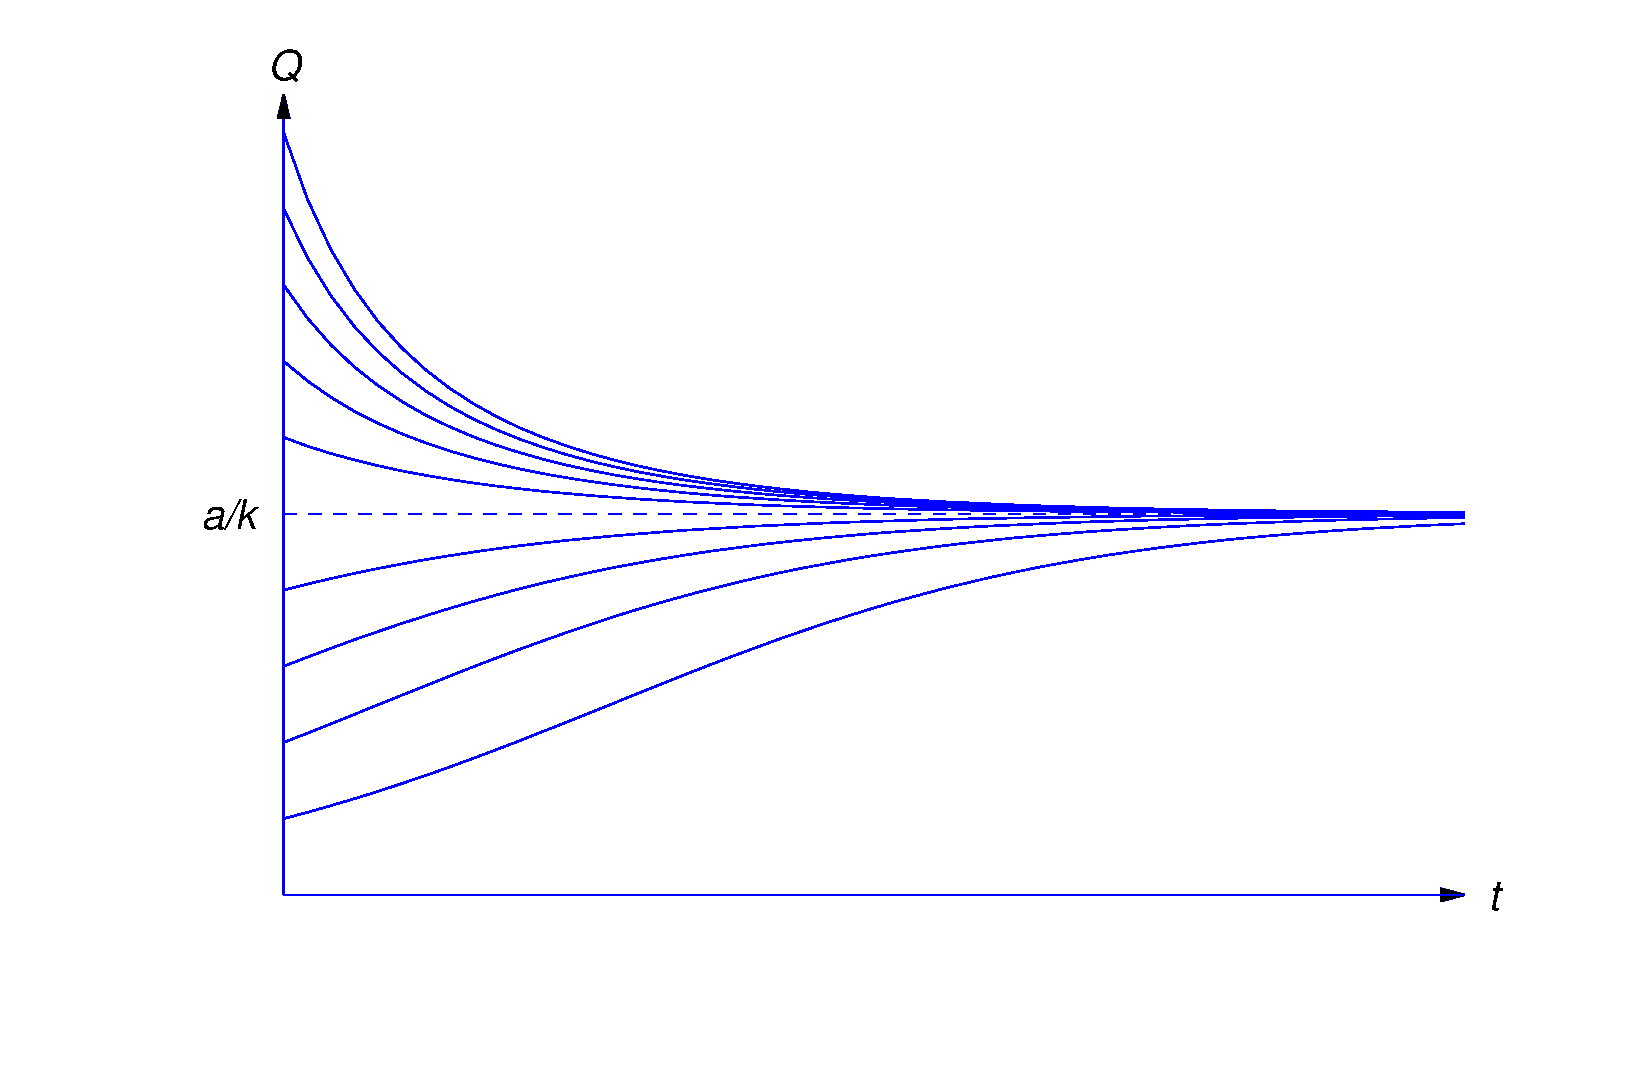
\includegraphics[bb=-78 148 689 643, width=5.67in, height=3.66in, keepaspectratio]{fig040103}
  \relax
  \caption{$Q(t)$ approaches the steady state value $\dst\frac{a}{k}$ as $t\to\infty$}
  \label{figure:4.1.3}
\end{figure}
\end{examplesolution}

\setcounter{example}{4}
\begin{example}
  \label{example:4.1.5} \rm An archaeologist investigating the site of an ancient village finds a
  burial ground where the amount of carbon-14 present in individual remains is between 42 and 44\%
  of the amount present in live individuals. Estimate the age of the village and the length of time
  for which it survived.
\end{example}
\begin{examplesolution}
\solution Let $Q=Q(t)$ be the quantity of carbon-14 in an individual set of remains $t$ years after
death, and let $Q_{0}$ be the quantity that would be present in live individuals. Since carbon-14
decays exponentially with half-life 5570 years, its decay constant is
\[
  k=\frac{\ln2}{5570}.
\]
Therefore
\[
  Q=Q_{0}e^{-t(\ln2)/5570}
\]
if we choose our time scale so that $t_{0}=0$ is the time of death. If we know the present value of
$Q$ we can solve this equation for $t$, the number of years since death occurred. This yields
\[
  t=-5570{\frac{\ln Q/Q_{0}}{\ln2}}.
\]
It is given that $Q=.42Q_{0}$ in the remains of individuals who died first. Therefore these deaths
occurred about
\[
  t_{1}=-5570{\frac{\ln.42}{\ln2}}\approx6971
\]
years ago. For the most recent deaths, $Q=.44 Q_{0}$; hence, these deaths occurred about
\[
  t_{2}=-5570{\frac{\ln.44}{\ln2}}\approx6597
\]
years ago. Therefore it's reasonable to conclude that the village was founded about 7000 years ago,
and lasted for about 400 years.
\end{examplesolution}

\setcounter{example}{5}
\begin{example}
  \label{example:4.1.6} \rm A person opens a savings account with an initial deposit of \$1000 and
  subsequently deposits \$50 per week. Find the value $Q(t)$ of the account at time $t>0$, assuming
  that the bank pays 6\% interest compounded continuously.
\end{example}
\setcounter{equation}{12}
\begin{examplesolution}
\solution Observe that $Q$ isn't continuous, since there are 52 discrete deposits per year of \$50
each. To construct a mathematical model for this problem in the form of a differential equation, we
make the simplifying assumption that the deposits are made continuously at a rate of \$2600 per
year. This is essential, since solutions of differential equations are continuous functions. With
this assumption, $Q$ increases continuously at the rate
\[
  Q'=2600+.06Q
\]
and therefore $Q$ satisfies the differential equation
\begin{equation}
  \label{eq:4.1.13}Q'-.06Q=2600.
\end{equation}
(Of course, we must recognize that the solution of this equation is an approximation to the true
value of $Q$ at any given time. We'll discuss this further below.) Since $e^{.06t}$ is a solution of
the complementary equation, the solutions of \eqref{eq:4.1.13} are of the form $Q=ue^{.06t}$, where
$u'e^{.06t}=2600$. Hence, $u'=2600e^{-.06t}$,
\[
  u=-\frac{2600}{.06}e^{-.06t}+c
\]
and
\begin{equation}
  \label{eq:4.1.14}Q=ue^{.06t}=-\frac{2600}{.06}+ce^{.06t}.
\end{equation}
Setting $t=0$ and $Q=1000$ here yields
\[
  c=1000+\frac{2600}{.06},
\]
and substituting this into \eqref{eq:4.1.14} yields
\begin{equation}
  \label{eq:4.1.15}Q=1000e^{.06t}+\frac{2600}{.06}(e^{.06t}-1),%\tag15
\end{equation}
where the first term is the value due to the initial deposit and the second is due to the subsequent
weekly deposits. \bbox
\end{examplesolution}

\section*{Section 4.2}
\setcounter{chapter}{4}
\setcounter{section}{2}

\setcounter{example}{0}
\begin{example}
  \label{example:4.2.1}\rm A ceramic insulator is baked at $400^{\circ}$C and cooled in a room in
  which the temperature is $25^{\circ}$C. After 4 minutes the temperature of the insulator is
  $200^{\circ}$C. What is its temperature after 8 minutes?
\end{example}
\setcounter{equation}{2}
\setcounter{figure}{0}
\begin{examplesolution}
\solution Here $T_{0}=400$ and $T_{m}=25$, so \textup{(4.2.2)} becomes
\begin{equation}
  \label{eq:4.2.3}T=25+375e^{-kt}.
\end{equation}
We determine $k$ from the stated condition that $T(4)=200$; that is,
\[
  200=25+375e^{-4k};
\]
hence,
\[
  e^{-4k}=\frac{175}{375}=\frac{7}{15}.
\]
Taking logarithms and solving for $k$ yields
\[
  k=-\frac{1}{4}\ln\frac{7}{15}=\frac{1}{4}\ln\frac{15}{7}.
\]
Substituting this into \eqref{eq:4.2.3} yields
\[
  T=25+375e^{-\frac{t}{4}\ln\frac{15}{7}}
\]
(Figure~\ref{figure:4.2.1}). Therefore the temperature of the insulator after 8 minutes is
\[
  \begin{array}{rl}
    T(8) & \dst=25+375e^{-2\ln\frac{15}{7}}                                     \\[9pt]
         & \dst=25+375\left(\frac{7}{15}\right)^{2}\approx 107^{\circ}\mbox{C}.
  \end{array}
\]

\begin{figure}[H]
  \centering
  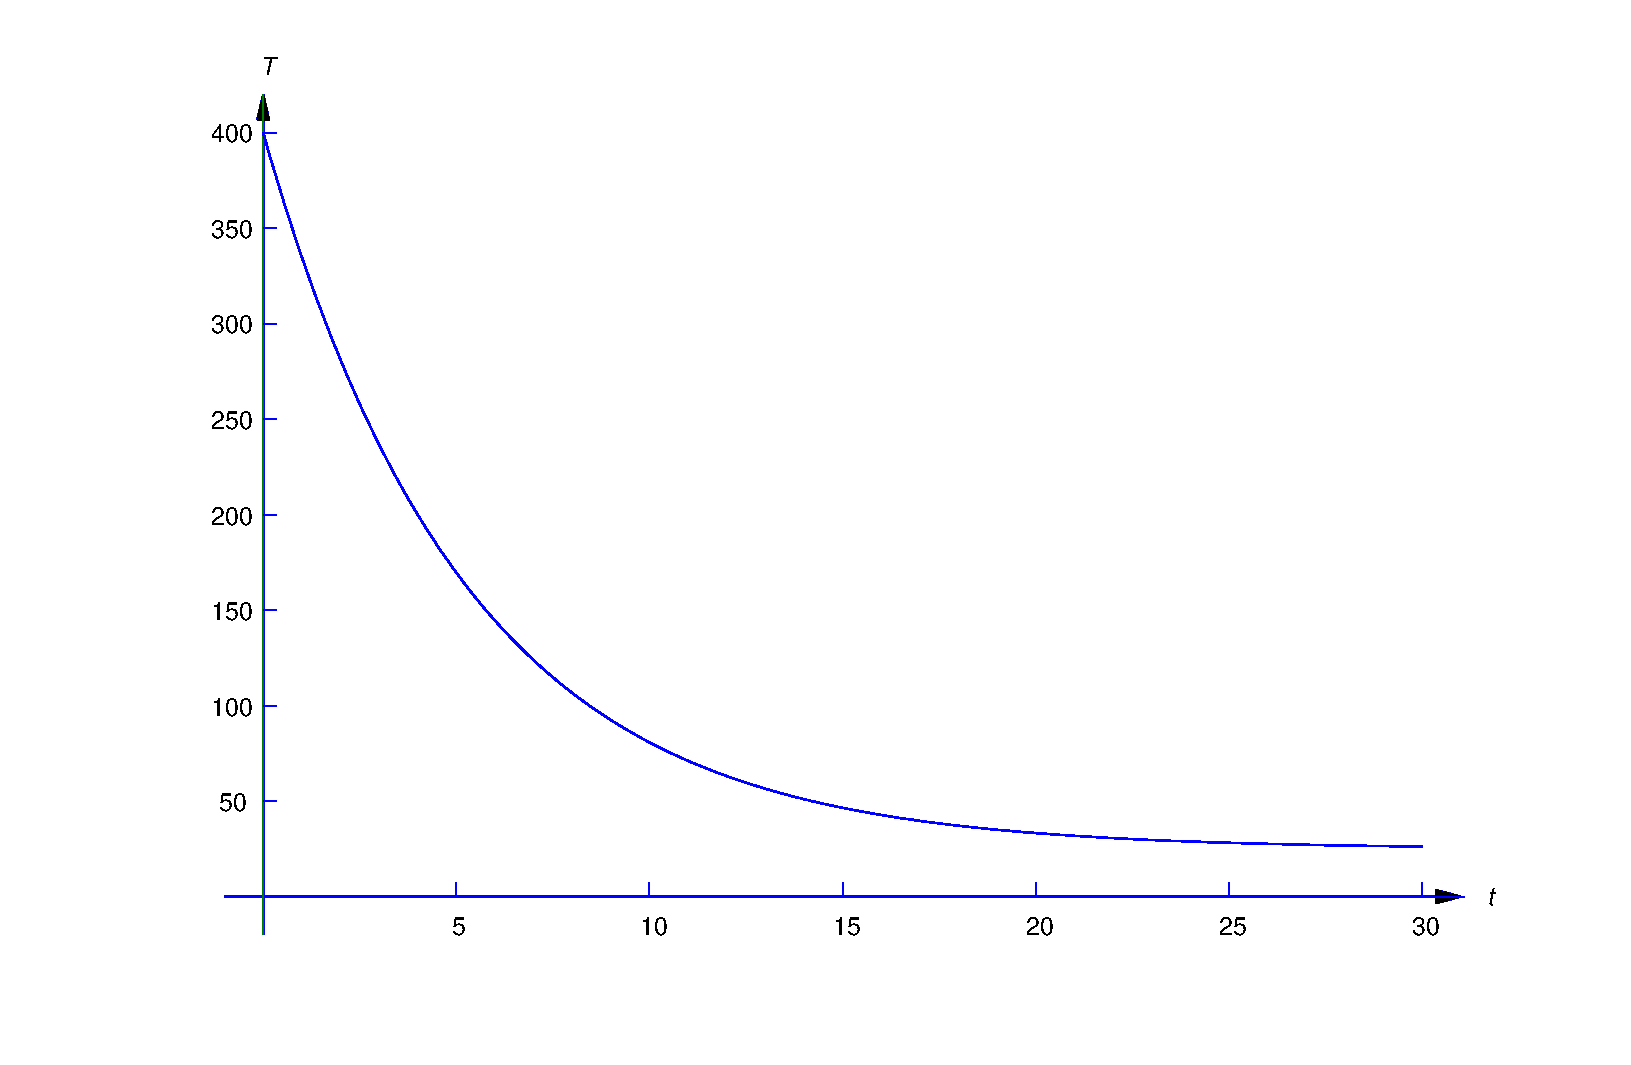
\includegraphics[bb=-78 148 689 643, width=5.67in, height=3.66in, keepaspectratio]{fig040201}
  \relax
  \caption{$T=25+375e^{-(t/4)\ln(15/7)}$}
  \label{figure:4.2.1}
\end{figure}
\end{examplesolution}

\setcounter{example}{1}
\begin{example}
  \label{example:4.2.2}\rm An object with temperature $72^{\circ}$F is placed outside, where the
  temperature is $-20^{\circ}$F. At 11:05 the temperature of the object is $60^{\circ}$F and at
  11:07 its temperature is $50^{\circ}$F. At what time was the object placed outside?
\end{example}
\setcounter{equation}{3}
\setcounter{figure}{1}
\begin{examplesolution}
\solution Let $T(t)$ be the temperature of the object at time $t$. For convenience, we choose the
origin $t_{0}=0$ of the time scale to be 11:05 so that $T_{0}=60$. We must determine the time $\tau$
when $T(\tau)=72$. Substituting $T_{0}=60$ and $T_{m}=-20$ into \textup{(4.2.2)} yields
\[
  T=-20+\bigl(60-(-20)\bigr)e^{-kt}
\]
or
\begin{equation}
  \label{eq:4.2.4}T=-20+80e^{-kt}.
\end{equation}
We obtain $k$ from the stated condition that the temperature of the object is 50$^{\circ}$F at
11:07. Since 11:07 is $t=2$ on our time scale, we can determine $k$ by substituting $T=50$ and $t=2$
into \eqref{eq:4.2.4} to obtain
\[
  50=-20+80e^{-2k}
\]
(Figure~\ref{figure:4.2.2}); hence,
\[
  e^{-2k}=\frac{70}{80}=\frac{7}{8}.
\]
Taking logarithms and solving for $k$ yields
\[
  k=-\frac{1}{2}\ln\frac{7}{8}=\frac{1}{2}\ln\frac{8}{7}.
\]
Substituting this into \eqref{eq:4.2.4} yields
\[
  T=-20+80e^{-\frac{t}{2}\ln\frac{8}{7}},
\]
and the condition $T(\tau)=72$ implies that
\[
  72=-20+80e^{-\frac{\tau}{2}\ln\frac{8}{7}};
\]
hence,
\[
  e^{-\frac{\tau}{2}\ln\frac{8}{7}}=\frac{92}{80}= \frac{23}{20}.
\]
Taking logarithms and solving for $\tau$ yields
\[
  \tau=-\frac{2\ln\frac{23}{20}}{\ln\frac{8}{7}}\approx-2.09\
\mbox{min}.
\]
Therefore the object was placed outside about 2 minutes and 5 seconds before 11:05; that is, at
11:02:55.

\begin{figure}[H]
  \centering
  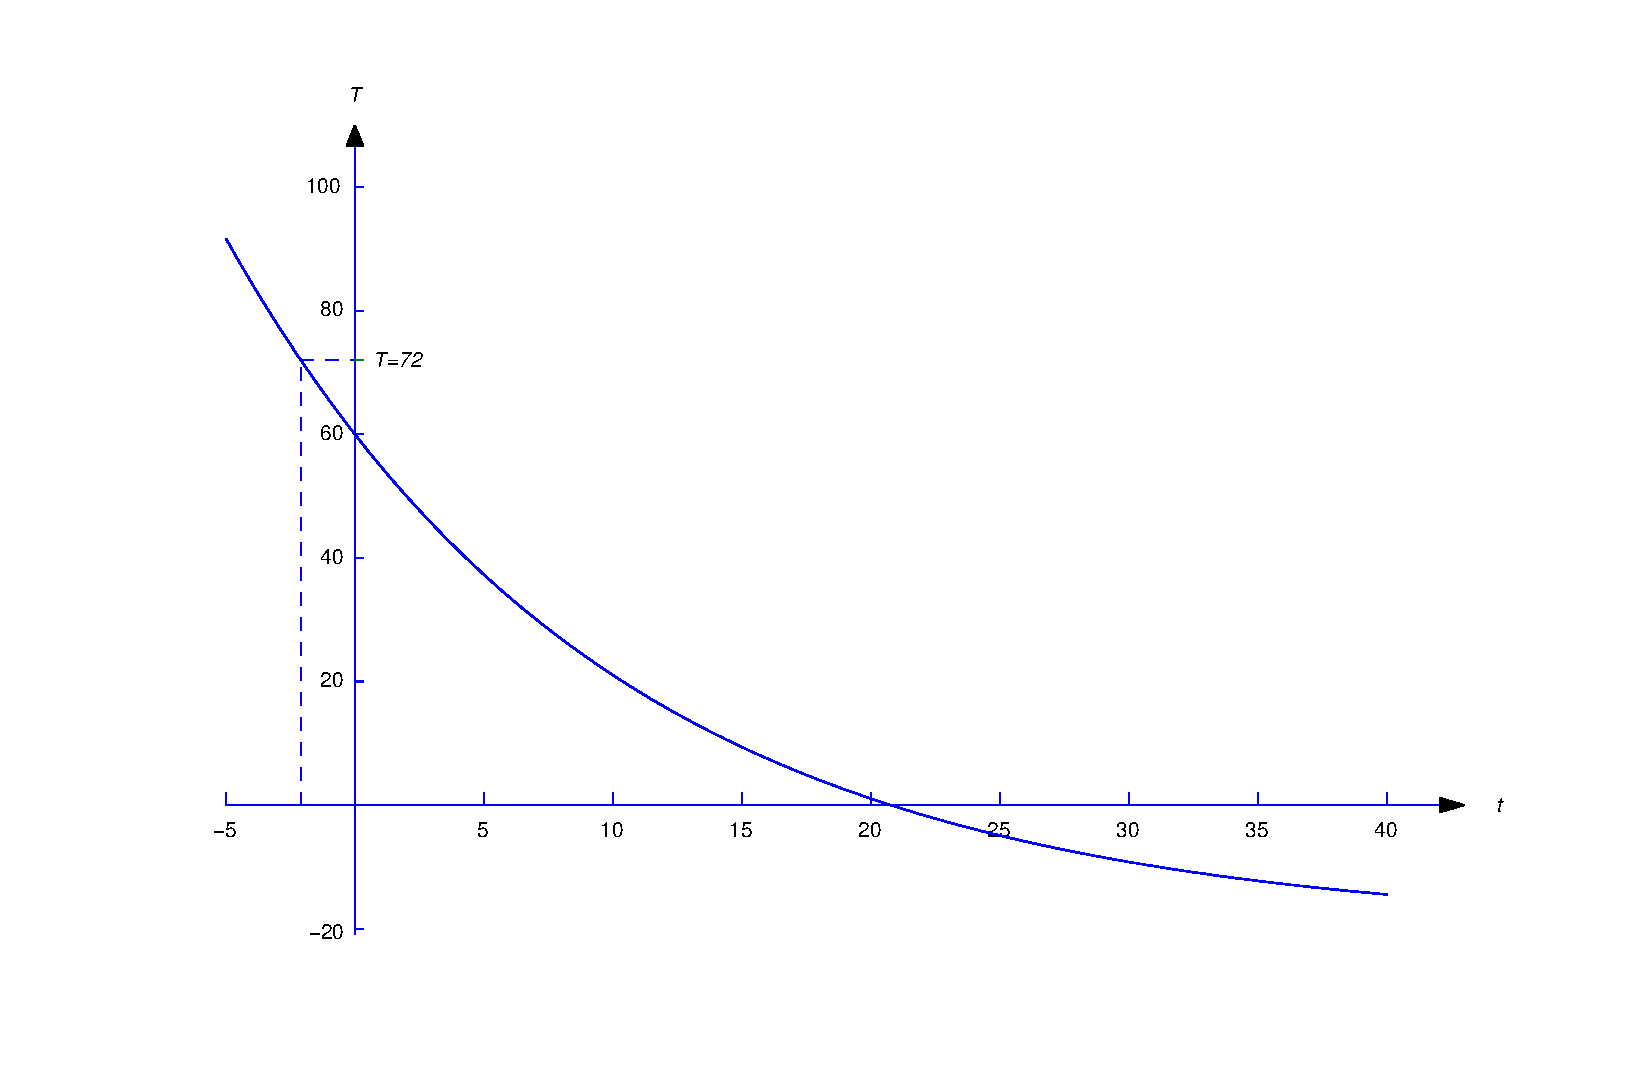
\includegraphics[bb=-78 148 689 643, width=5.67in, height=3.66in, keepaspectratio]{fig040202}
  \relax
  \caption{$T=-20+80e^{-\frac{t}{2}\ln\frac{8}{7}}$}
  \label{figure:4.2.2}
\end{figure}
\end{examplesolution}

\setcounter{example}{2}
\begin{example}
  \label{example:4.2.3} \rm A tank initially contains 40 pounds of salt dissolved in 600 gallons of
  water. Starting at $t_{0}=0$, water that contains 1/2 pound of salt per gallon is poured into the
  tank at the rate of 4 gal/min and the mixture is drained from the tank at the same rate
  (Figure~4.2.3).
  \begin{alist}
    \item % (a)
    Find a differential equation for the quantity $Q(t)$ of salt in the tank at time $t>0$, and
    solve the equation to determine $Q(t)$.

    \item % (b)
    Find $\lim_{t\to\infty}Q(t)$.
  \end{alist}
\end{example}
\setcounter{equation}{4}
\begin{examplesolution}
\solutionpart{a} To find a differential equation for $Q$, we must use the given information to
derive an expression for $Q'$. But $Q'$ is the rate at which the quantity of salt in the tank
changes with respect to time; thus, if {\relax\it rate in\/} denotes the rate at which salt
enters the tank and {\relax\it rate out\/} denotes the rate by which it leaves, then
\begin{equation}
  \label{eq:4.2.5}Q'=\mbox{rate in}-\mbox{rate out}.
\end{equation}
The rate in is
\[
  \left(\frac{1}{2}\ \mbox{lb/gal}\right)\times(4\ \mbox{gal/min})=2\
\mbox{lb/min}.
\]
Determining the rate out requires a little more thought. We're removing 4 gallons of the mixture per
minute, and there are always 600 gallons in the tank; that is, we're removing $1/150$ of the mixture
per minute. Since the salt is evenly distributed in the mixture, we are also removing $1/150$ of the
salt per minute. Therefore, if there are $Q(t)$ pounds of salt in the tank at time $t$, the rate out
at any time $t$ is $Q(t)/150$. Alternatively, we can arrive at this conclusion by arguing that
\[
  \begin{array}{lcl}
    \mbox{rate out} & = & (\mbox{concentration})\times(\mbox{rate of flow out}) \\[6pt]
    \mbox{}         & = & (\mbox{lb/gal})\times(\mbox{gal/min})                 \\[10pt]
                    & = & \dst\frac{Q(t)}{600}\times 4=\dst\frac{Q(t)}{150}.
  \end{array}
\]
We can now write \eqref{eq:4.2.5} as
\[
  Q'=2-\frac{Q}{150}.
\]
This first order equation can be rewritten as
\[
  Q'+\frac{Q}{150}=2.
\]
Since $e^{-t/150}$ is a solution of the complementary equation, the solutions of this equation are
of the form $Q=ue^{-t/150}$, where $u'e^{-t/150}=2$, so $u'=2e^{t/150}$. Hence,
\[
  u=300e^{t/150}+c,
\]
so
\begin{equation}
  \label{eq:4.2.6}Q=ue^{-t/150}=300+ce^{-t/150}
\end{equation}
(Figure~4.2.4). Since $Q(0)=40$, $c=-260$; therefore,
\[
  Q=300-260e^{-t/150}.
\]

\solutionpart{b} From \eqref{eq:4.2.6}, we see that $\lim_{t\to \infty}Q(t)=300$ for any value
of $Q(0)$. This is intuitively reasonable, since the incoming solution contains 1/2 pound of salt
per gallon and there are always 600 gallons of water in the tank. \quad
\end{examplesolution}

\setcounter{example}{3}
\begin{example}
  \label{example:4.2.4} \rm A 500-liter tank initially contains 10 g of salt dissolved in 200 liters
  of water. Starting at $t_{0}=0$, water that contains 1/4 g of salt per liter is poured into the
  tank at the rate of 4 liters/min and the mixture is drained from the tank at the rate of 2
  liters/min (Figure~4.2.5). Find a differential equation for the quantity $Q(t)$ of
  salt in the tank at time $t$ prior to the time when the tank overflows and find the concentration
  $K(t)$ (g/liter ) of salt in the tank at any such time.
\end{example}
\setcounter{equation}{6}
\setcounter{figure}{5}
\begin{examplesolution}
\solution We first determine the amount $W(t)$ of solution in the tank at any time $t$ prior to
overflow. Since $W(0)=200$ and we're adding 4 liters/min while removing only 2 liters/min, there's a
net gain of 2 liters/min in the tank; therefore,
\[
  W(t)=2t+200.
\]
Since $W(150)=500$ liters (capacity of the tank), this formula is valid for $0\le t\le150$.

Now let $Q(t)$ be the number of grams of salt in the tank at time $t$, where $0\le t\le150$. As in
Example~\ref{example:4.2.3},
\begin{equation}
  \label{eq:4.2.7}Q'=\mbox{rate in}-\mbox{rate out}.
\end{equation}
The rate in is
\begin{equation}
  \label{eq:4.2.8}\left(\frac{1}{4}\ \mbox{g/liter}\,\right)\times(4\
\mbox{liters/min}\,)=1\ \mbox{g/min}.
\end{equation}
To determine the rate out, we observe that since the mixture is being removed from the tank at the
constant rate of 2 liters/min and there are $2t+200$ liters in the tank at time $t$, the fraction of
the mixture being removed per minute at time $t$ is
\[
  \frac{2}{2t+200}=\frac{1}{t+100}.
\]
We're removing this same fraction of the salt per minute. Therefore, since there are $Q(t)$ grams of
salt in the tank at time $t$,
\begin{equation}
  \label{eq:4.2.9}\mbox{rate out}=\frac{Q(t)}{t+100}.
\end{equation}
Alternatively, we can arrive at this conclusion by arguing that
\[
  \begin{array}{lcl}
    \mbox{rate out} & = & (\mbox{concentration})\times(\mbox{rate of flow out}) =(\mbox{g/liter})\times(\mbox{liters/min}) \\[10pt]
                    & = & \dst\frac{Q(t)}{2t+200}\times 2=\dst\frac{Q(t)}{t+100}.
  \end{array}
\]
Substituting \eqref{eq:4.2.8} and \eqref{eq:4.2.9} into \eqref{eq:4.2.7} yields
\begin{equation}
  \label{eq:4.2.10}Q'=1-\frac{Q}{t+100},\quad\text{ \rm so }\quad Q'+\frac{1}{t+100}Q=1.
\end{equation}
By separation of variables, $1/(t+100)$ is a solution of the complementary equation, so the
solutions of \eqref{eq:4.2.10} are of the form
\[
  Q=\frac{u}{t+100},\mbox{\quad where \quad}{\frac{u'}{t+100}}=1,\mbox{\quad so \quad}u'=t+100.
\]
Hence,
\begin{equation}
  \label{eq:4.2.11}u=\frac{(t+100)^{2}}{2}+c.
\end{equation}
Since $Q(0)=10$ and $u=(t+100)Q$, \eqref{eq:4.2.11} implies that
\[
  (100)(10)=\frac{(100)^{2}}{2}+c,
\]
so
\[
  c=100(10)-\frac{(100)^{2}}{2}=-4000
\]
and therefore
\[
  u=\frac{(t+100)^{2}}{2}-4000.
\]
Hence,
\[
  Q=\frac{u}{t+100}=\frac{t+100}{2}-\frac{4000}{t+100}.
\]
Now let $K(t)$ be the concentration of salt at time $t$. Then
\[
  K(t)=\frac{1}{4}-\frac{2000}{(t+100)^{2}}
\]
(Figure~\ref{figure:4.2.6}).
\begin{figure}[H]
  \centering
  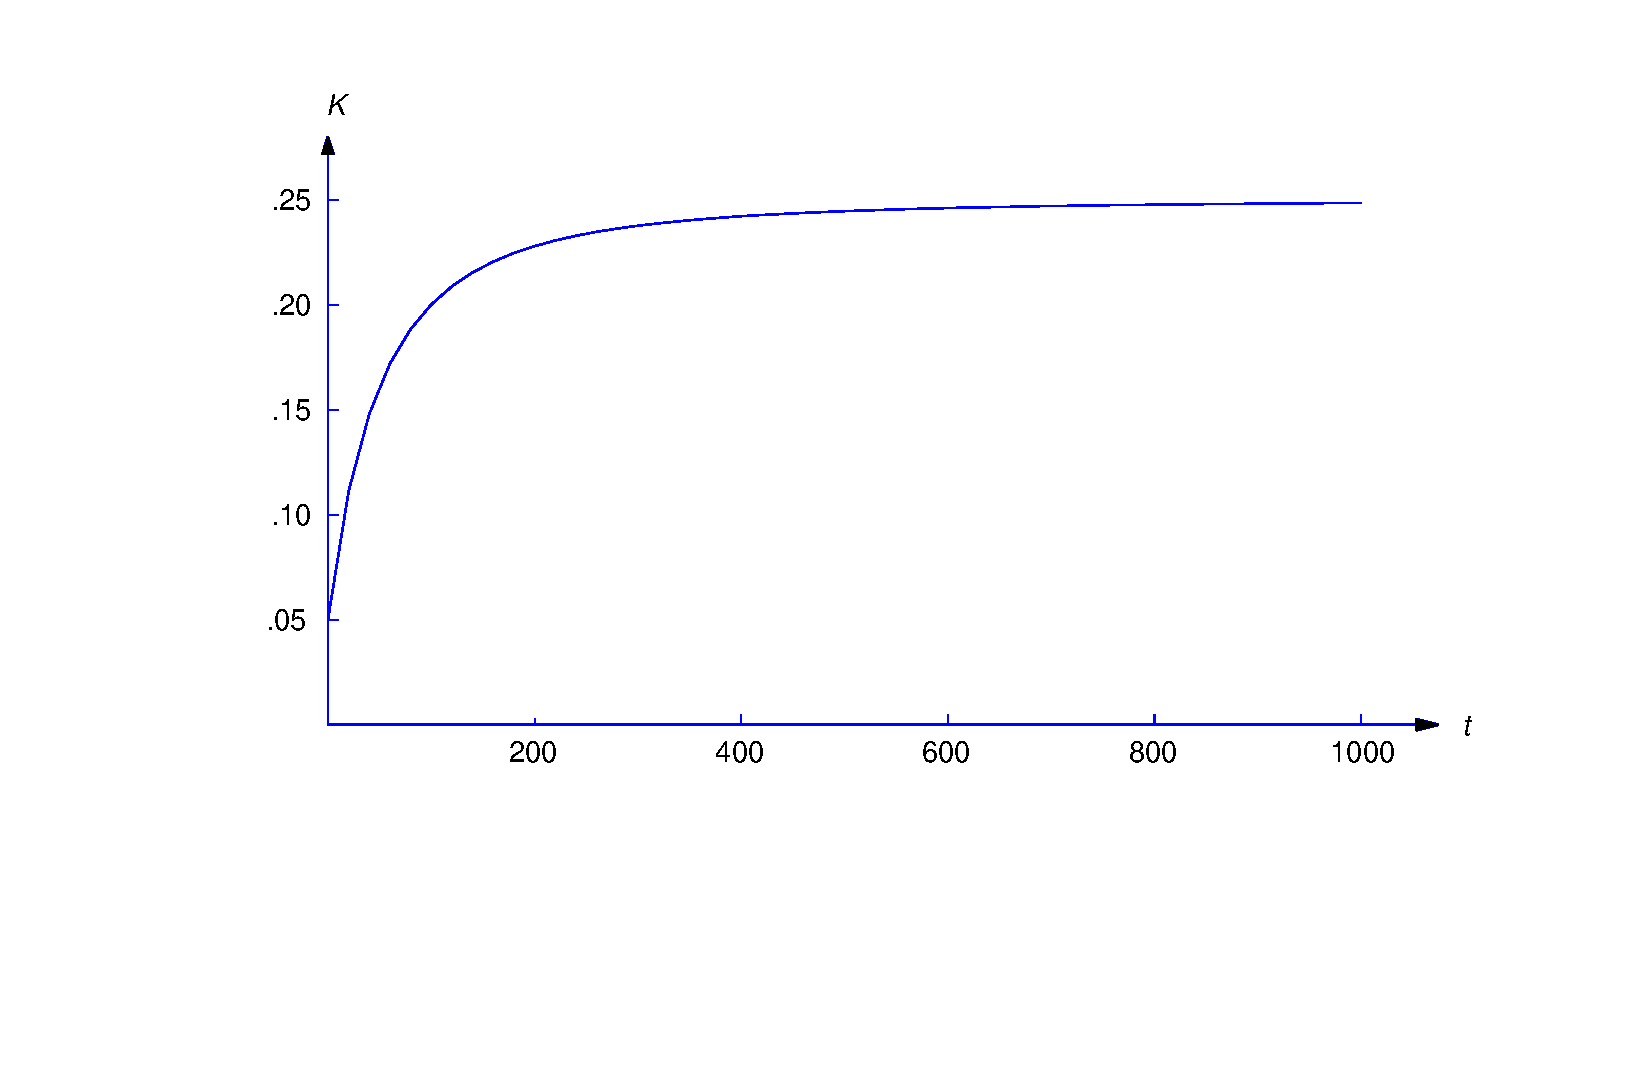
\includegraphics[bb=-78 148 689 643, width=5.67in, height=3.66in, keepaspectratio]{fig040206}
  \relax
  \caption{$K(t)=\dst{\frac{1}{4}-\frac{2000}{(t+100)^{2}}}$}
  \label{figure:4.2.6}
\end{figure}
\end{examplesolution}

\section*{Section 4.3}
\setcounter{chapter}{4}
\setcounter{section}{3}

\setcounter{example}{0}
\begin{example}
  \label{example:4.3.1} \rm An object with mass $m$ moves under constant gravitational force through
  a medium that exerts a resistance with magnitude proportional to the speed of the object. (Recall
  that the speed of an object is $|v|$, the absolute value of its velocity $v$.) Find the velocity
  of the object as a function of $t$, and find the terminal velocity. Assume that the initial
  velocity is $v_{0}$.
\end{example}
\setcounter{equation}{3}
\setcounter{figure}{0}
\begin{examplesolution}
\solution The total force acting on the object is
\begin{equation}
  \label{eq:4.3.4}F=-mg+F_{1},
\end{equation}
where $-mg$ is the force due to gravity and $F_{1}$ is the resisting force of the medium, which has
magnitude $k|v|$, where $k$ is a positive constant. If the object is moving downward ($v\le0$), the
resisting force is upward (Figure~\ref{figure:4.3.1}\part{a}), so
\[
  F_{1}=k|v|=k(-v)=-kv.
\]
On the other hand, if the object is moving upward ($v\ge0$), the resisting force is downward
(Figure~\ref{figure:4.3.1}\part{b}), so
\[
  F_{1}=-k|v|=-kv.
\]
Thus, (\ref{eq:4.3.4}) can be written as
\begin{equation}
  \label{eq:4.3.5}F=-mg-kv,
\end{equation}
regardless of the sign of the velocity.

\begin{figure}[H]
  \centering
  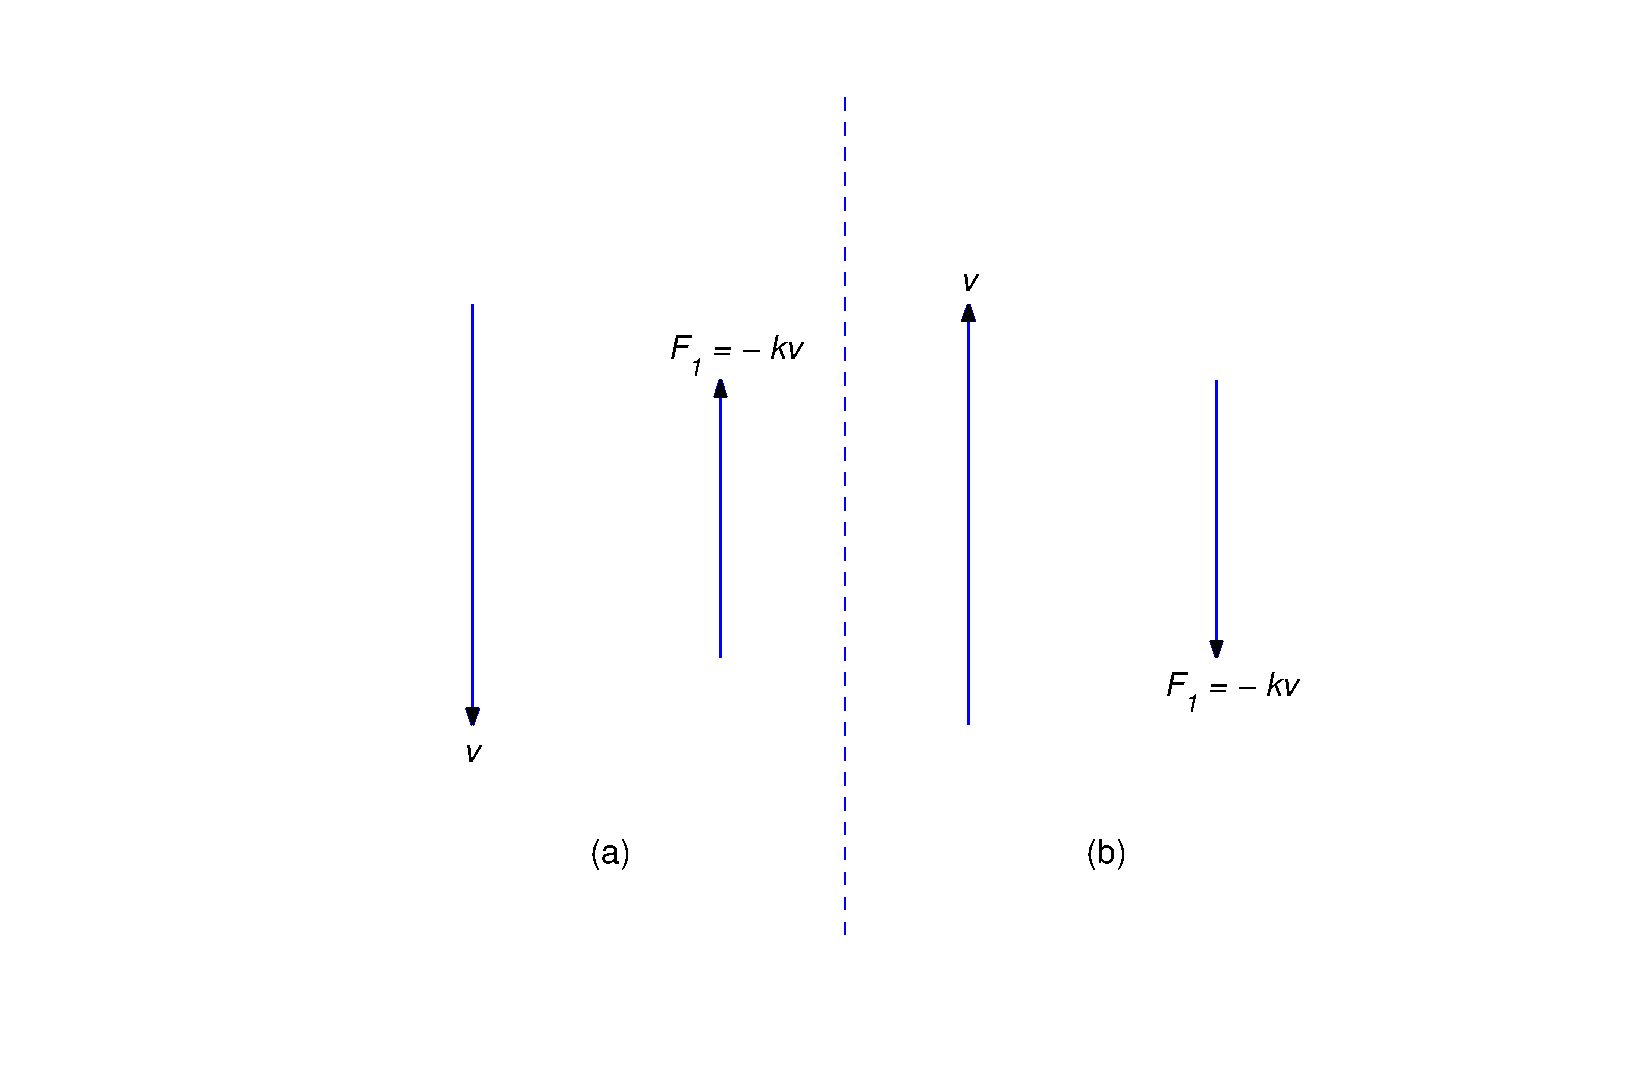
\includegraphics[bb=-78 148 689 643, width=5.67in, height=3.66in, keepaspectratio]{fig040301}
  \relax
  \caption{Resistive forces}
  \label{figure:4.3.1}
\end{figure}

From Newton's second law of motion,
\[
  F=ma=mv',
\]
so (\ref{eq:4.3.5}) yields
\[
  mv'=-mg-kv,
\]
or
\begin{equation}
  \label{eq:4.3.6}v'+\frac{k}{m}v=-g.
\end{equation}
Since $e^{-kt/m}$ is a solution of the complementary equation, the solutions of (\ref{eq:4.3.6}) are
of the form $v=ue^{-kt/m}$, where $u'e^{-kt/m}=-g$, so $u'=-ge^{kt/m}$. Hence,
\[
  u=-\frac{mg}{k}e^{kt/m}+c,
\]
so
\begin{equation}
  \label{eq:4.3.7}v=ue^{-kt/m}=-\frac{mg}{k}+ce^{-kt/m}.
\end{equation}
Since $v(0)=v_{0}$,
\[
  v_{0}=-\frac{mg}{k}+c,
\]
so
\[
  c=v_{0}+\frac{mg}{k}
\]
and (\ref{eq:4.3.7}) becomes
\[
  v=-\frac{mg}{k}+\left(v_{0}+\frac{mg}{k}\right)e^{-kt/m}.
\]
Letting $t\to\infty$ here shows that the terminal velocity is
\[
  \lim_{t\to\infty}v(t)=-\frac{mg}{k},
\]
which is independent of the initial velocity $v_{0}$ (Figure~\ref{figure:4.3.2}).

\begin{figure}[H]
  \centering
  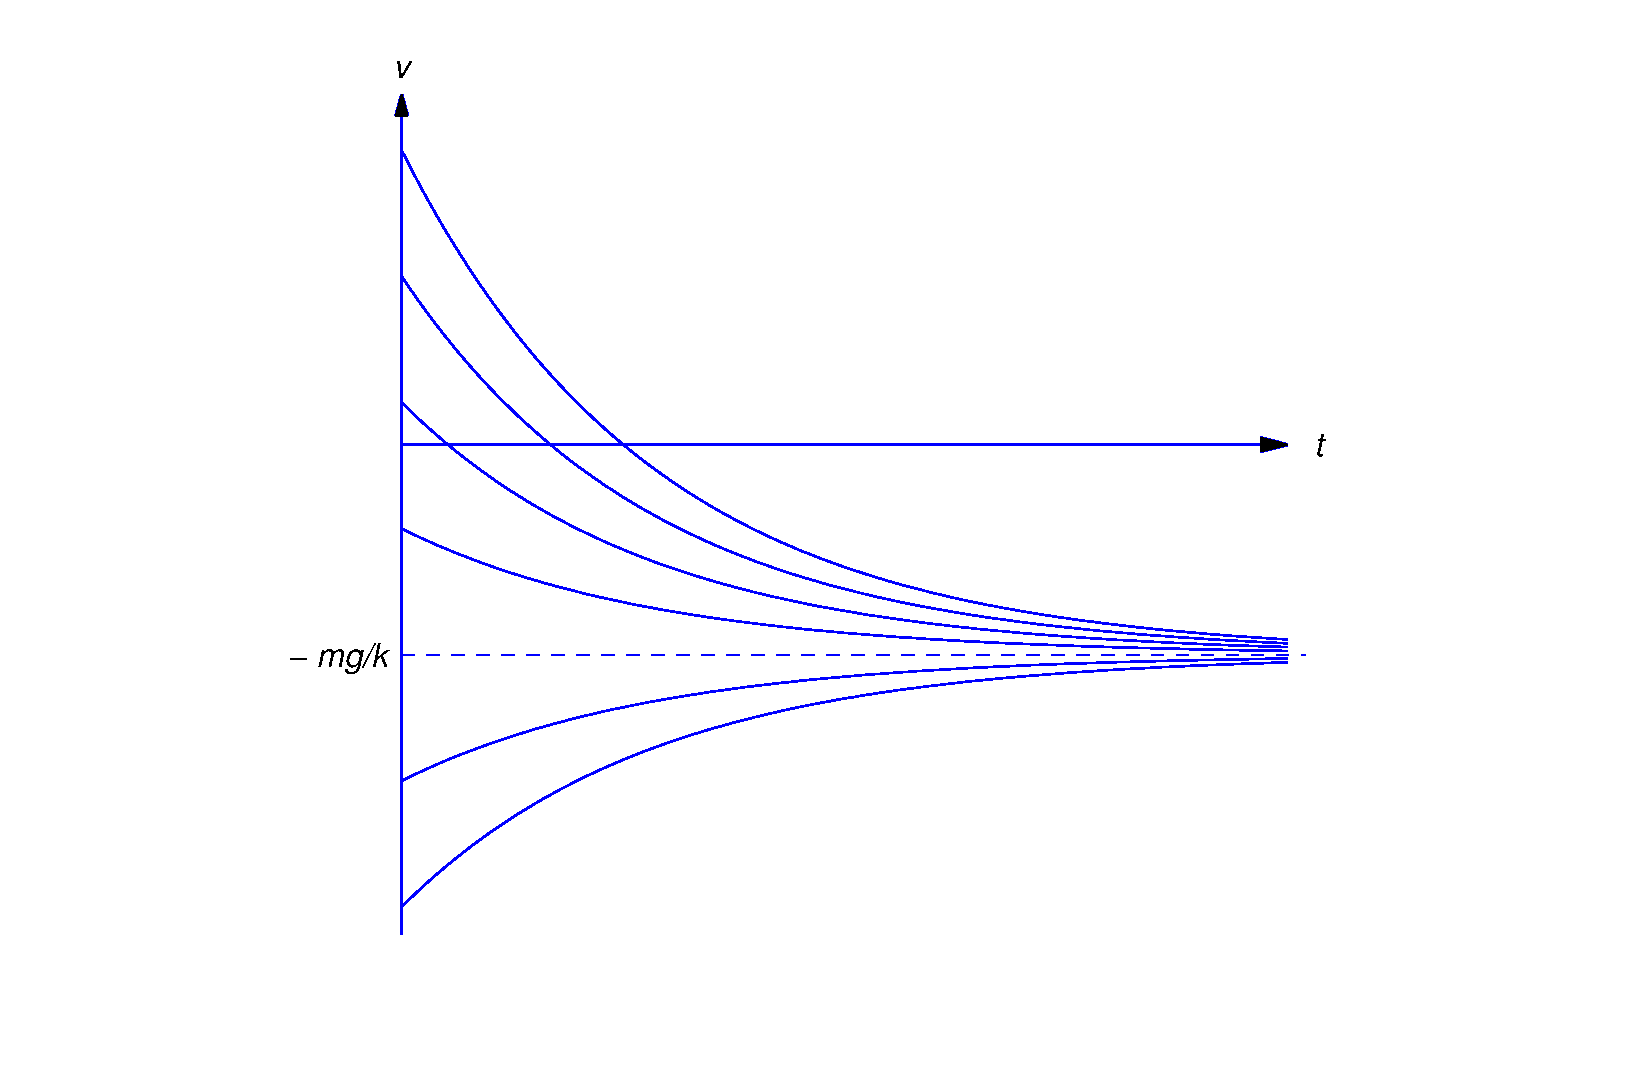
\includegraphics[bb=-78 148 689 643, width=5.67in, height=3.66in, keepaspectratio]{fig040302}
  \relax
  \caption{Solutions of $mv'=-mg-kv$}
  \label{figure:4.3.2}
\end{figure}
\end{examplesolution}

\setcounter{example}{1}
\begin{example}
  \label{example:4.3.2} \rm A 960-lb object is given an initial upward velocity of 60 ft/s near the
  surface of Earth. The atmosphere resists the motion with a force of 3 lb for each ft/s of speed.
  Assuming that the only other force acting on the object is constant gravity, find its velocity $v$
  as a function of $t$, and find its terminal velocity.
\end{example}
\setcounter{equation}{7}
\begin{examplesolution}
\solution Since $mg=960$ and $g=32$, $m=960/32=30$. The atmospheric resistance is $-3v$ lb if $v$ is
expressed in feet per second. Therefore
\[
  30v'=-960-3v,
\]
which we rewrite as
\[
  v'+\frac{1}{10}v=-32.
\]
Since $e^{-t/10}$ is a solution of the complementary equation, the solutions of this equation are of
the form $v=ue^{-t/10}$, where $u'e^{-t/10}=-32$, so $u'=-32e^{t/10}$. Hence,
\[
  u=-320e^{t/10}+c,
\]
so
\begin{equation}
  \label{eq:4.3.8}v=ue^{-t/10}=-320+ce^{-t/10}.
\end{equation}
The initial velocity is 60 ft/s in the upward (positive) direction; hence, $v_{0}=60$. Substituting
$t=0$ and $v=60$ in (\ref{eq:4.3.8}) yields
\[
  60=-320+c,
\]
so $c=380$, and (\ref{eq:4.3.8}) becomes
\[
  v=-320+380e^{-t/10}\ \mbox{ft/s}
\]
The terminal velocity is
\[
  \lim_{t\to\infty}v(t)=-320\mbox{ ft/s.}
\]
\end{examplesolution}

\setcounter{example}{2}
\begin{example}
  \label{example:4.3.3} \rm A 10 kg mass is given an initial velocity $v_{0}\le0$ near Earth's
  surface. The only forces acting on it are gravity and atmospheric resistance proportional to the
  square of the speed. Assuming that the resistance is 8 N if the speed is 2 m/s, find the velocity
  of the object as a function of $t$, and find the terminal velocity.
\end{example}
\setcounter{equation}{8}
\setcounter{figure}{2}
\begin{examplesolution}
\solution Since the object is falling, the resistance is in the upward (positive) direction. Hence,
\begin{equation}
  \label{eq:4.3.9}mv'=-mg+kv^{2},
\end{equation}
where $k$ is a constant. Since the magnitude of the resistance is 8 N when $v=2$ m/s,
\[
  k(2^{2})=8,
\]
so $k=2\ \mbox{N-s}^{2}/\mbox{m}^{2}$. Since $m=10$ and $g=9.8$, (\ref{eq:4.3.9}) becomes
\begin{equation}
  \label{eq:4.3.10}10v'=-98+2v^{2}=2(v^{2}-49).
\end{equation}
If $v_{0}=-7$, then $v\equiv-7$ for all $t\ge0$. If $v_{0}\ne-7$, we separate variables to obtain
\begin{equation}
  \label{eq:4.3.11}\frac{1}{v^{2}-49}v'=\frac{1}{5},
\end{equation}
which is convenient for the required partial fraction expansion
\begin{equation}
  \label{eq:4.3.12}\frac{1}{v^{2}-49}=\frac{1}{(v-7)(v+7)}=\frac{1}{14}\left[\frac{1}{v-7}-\frac{1}{v+7}\right].
\end{equation}
Substituting (\ref{eq:4.3.12}) into (\ref{eq:4.3.11}) yields
\[
  \frac{1}{14}\left[\frac{1}{v-7}-\frac{1}{v+7}\right]v'=\frac{1}{5},
\]
so
\[
  \left[\frac{1}{v-7}-\frac{1}{v+7}\right]v'=\frac{14}{5}.
\]
Integrating this yields
\[
  \ln|v-7|-\ln|v+7|=14t/5+C.
\]
Therefore
\[
  \left|\frac{v-7}{v+7}\right|=e^{C}e^{14t/5}.
\]
Since Theorem~2.3.1 implies that $(v-7)/(v+7)$ can't change sign (why?), we can
rewrite the last equation as
\begin{equation}
  \label{eq:4.3.13}\frac{v-7}{v+7}=ce^{14t/5},
\end{equation}
which is an implicit solution of (\ref{eq:4.3.10}). Solving this for $v$ yields
\begin{equation}
  \label{eq:4.3.14}v=-7{\frac{c+e^{-14t/5}}{c-e^{-14t/5}}}.
\end{equation}
Since $v(0)=v_{0}$, (\ref{eq:4.3.13}) implies that
\[
  c=\frac{v_{0}-7}{v_{0}+7}.
\]
Substituting this into (\ref{eq:4.3.14}) and simplifying yields
\[
  v=-7{\frac{v_{0}(1+e^{-14t/5})-7(1-e^{-14t/5})}{v_{0}(1-e^{-14t/5})-7(1+e^{-14t/5})}}.
\]
Since $v_{0}\le0$, $v$ is defined and negative for all $t>0$. The terminal velocity is
\[
  \lim_{t\to\infty}v(t)=-7\ \mbox{m/s},
\]
independent of $v_{0}$. More generally, it can be shown (Exercise~4.3.11) that if $v$ is
any solution of (\ref{eq:4.3.9}) such that $v_{0}\le0$ then
\[
  \lim_{t\to\infty}v(t)=-\sqrt{\frac{mg}{k}}
\]
(Figure~\ref{figure:4.3.3}).

\begin{figure}[H]
  \centering
  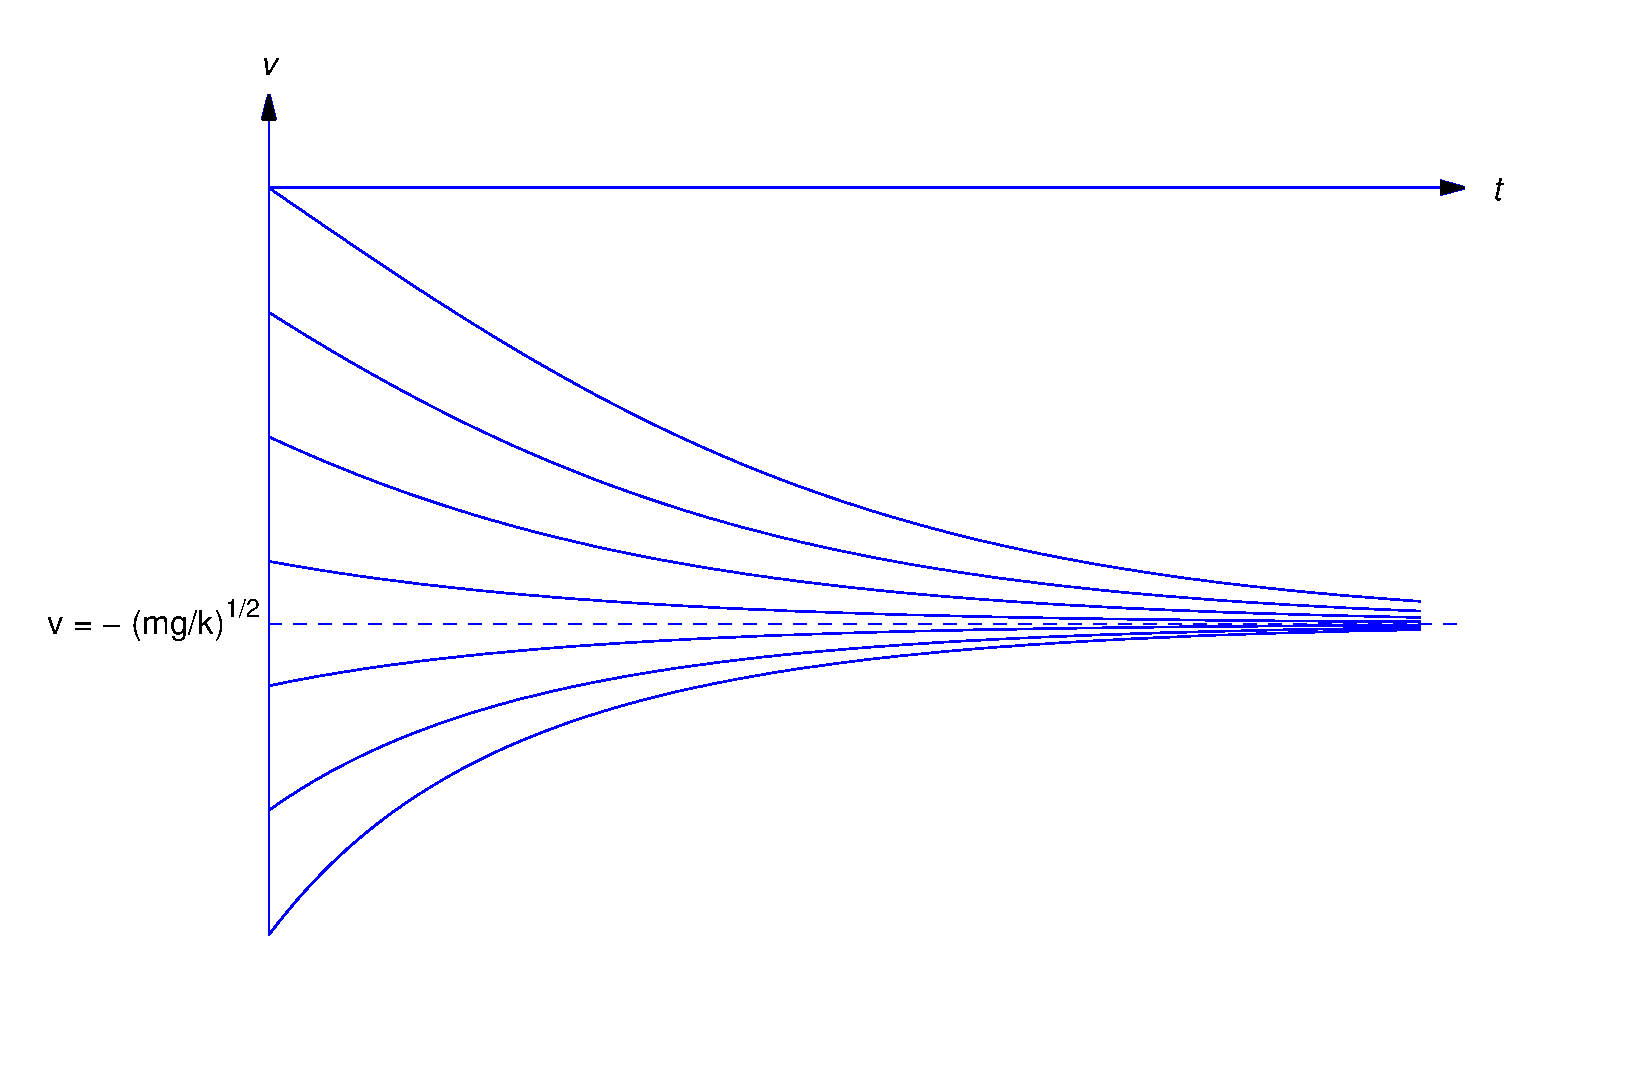
\includegraphics[bb=-78 148 689 643, width=5.67in, height=3.66in, keepaspectratio]{fig040303}
  \relax
  \caption{Solutions of $mv'=-mg+kv^{2}$, $v(0)=v_{0}\le0$}
  \label{figure:4.3.3}
\end{figure}
\end{examplesolution}

\setcounter{example}{3}
\begin{example}
  \label{example:4.3.4} \rm A 10-kg mass is launched vertically upward from Earth's surface with an
  initial velocity of $v_{0}$ m/s. The only forces acting on the mass are gravity and atmospheric
  resistance proportional to the square of the speed. Assuming that the atmospheric resistance is 8
  N if the speed is 2 m/s, find the time $T$ required for the mass to reach maximum altitude.
\end{example}
\setcounter{equation}{14}
\setcounter{figure}{3}
\begin{examplesolution}
\solution The mass will climb while $v>0$ and reach its maximum altitude when $v=0$. Therefore $v>0$
for $0\le t<T$ and $v(T)=0$. Although the mass of the object and our assumptions concerning the
forces acting on it are the same as those in Example 3, (\ref{eq:4.3.10}) does not apply here, since
the resisting force is negative if $v>0$; therefore, we replace (\ref{eq:4.3.10}) by
\begin{equation}
  \label{eq:4.3.15}10v'=-98-2v^{2}.
\end{equation}

Separating variables yields
\[
  \frac{5}{v^{2}+49}v'=-1,
\]
and integrating this yields
\[
  \frac{5}{7}\tan^{-1}\frac{v}{7}=-t+c.
\]
(Recall that $\tan^{-1}u$ is the number $\theta$ such that $-\pi/2<\theta<\pi/2$ and
$\tan\theta=u$.) Since $v(0)=v_{0}$,
\[
  c=\frac{5}{7}\tan^{-1}\frac{v_{0}}{7},
\]
so $v$ is defined implicitly by
\begin{equation}
  \label{eq:4.3.16}\frac{5}{7}\tan^{-1}\frac{v}{7}=-t+\frac{5}{7}\tan^{-1}\frac{v_{0}}{7},\quad0\le t\le T.
\end{equation}
Solving this for $v$ yields
\begin{equation}
  \label{eq:4.3.17}v=7\tan\left(-\frac{7t}{5}+\tan^{-1}\frac{v_{0}}{7}\right).
\end{equation}
Using the identity
\[
  \tan(A-B)=\frac{\tan A-\tan B}{1+\tan A\tan B}
\]
with $A=\tan^{-1}(v_{0}/7)$ and $B=7t/5$, and noting that $\tan(\tan^{-1}\theta)=\theta$, we can
simplify (\ref{eq:4.3.17}) to
\[
  v=7{\frac{v_{0}-7\tan(7t/5)}{7+v_{0}\tan(7t/5)}}.
\]

Since $v(T)=0$ and $\tan^{-1}(0)=0$, (\ref{eq:4.3.16}) implies that
\[
  -T+\frac{5}{7}\tan^{-1}\frac{v_{0}}{7}=0.
\]
Therefore
\[
  T=\frac{5}{7}\tan^{-1}\frac{v_{0}}{7}.
\]
Since $\tan^{-1}(v_{0}/7)<\pi/2$ for all $v_{0}$, the time required for the mass to reach its
maximum altitude is less than
\[
  \frac{5\pi}{14}\approx1.122\ \mbox{s}
\]
regardless of the initial velocity. Figure~\ref{figure:4.3.4} shows graphs of $v$ over $[0,T]$ for
various values of $v_{0}$.

\begin{figure}[H]
  \centering
  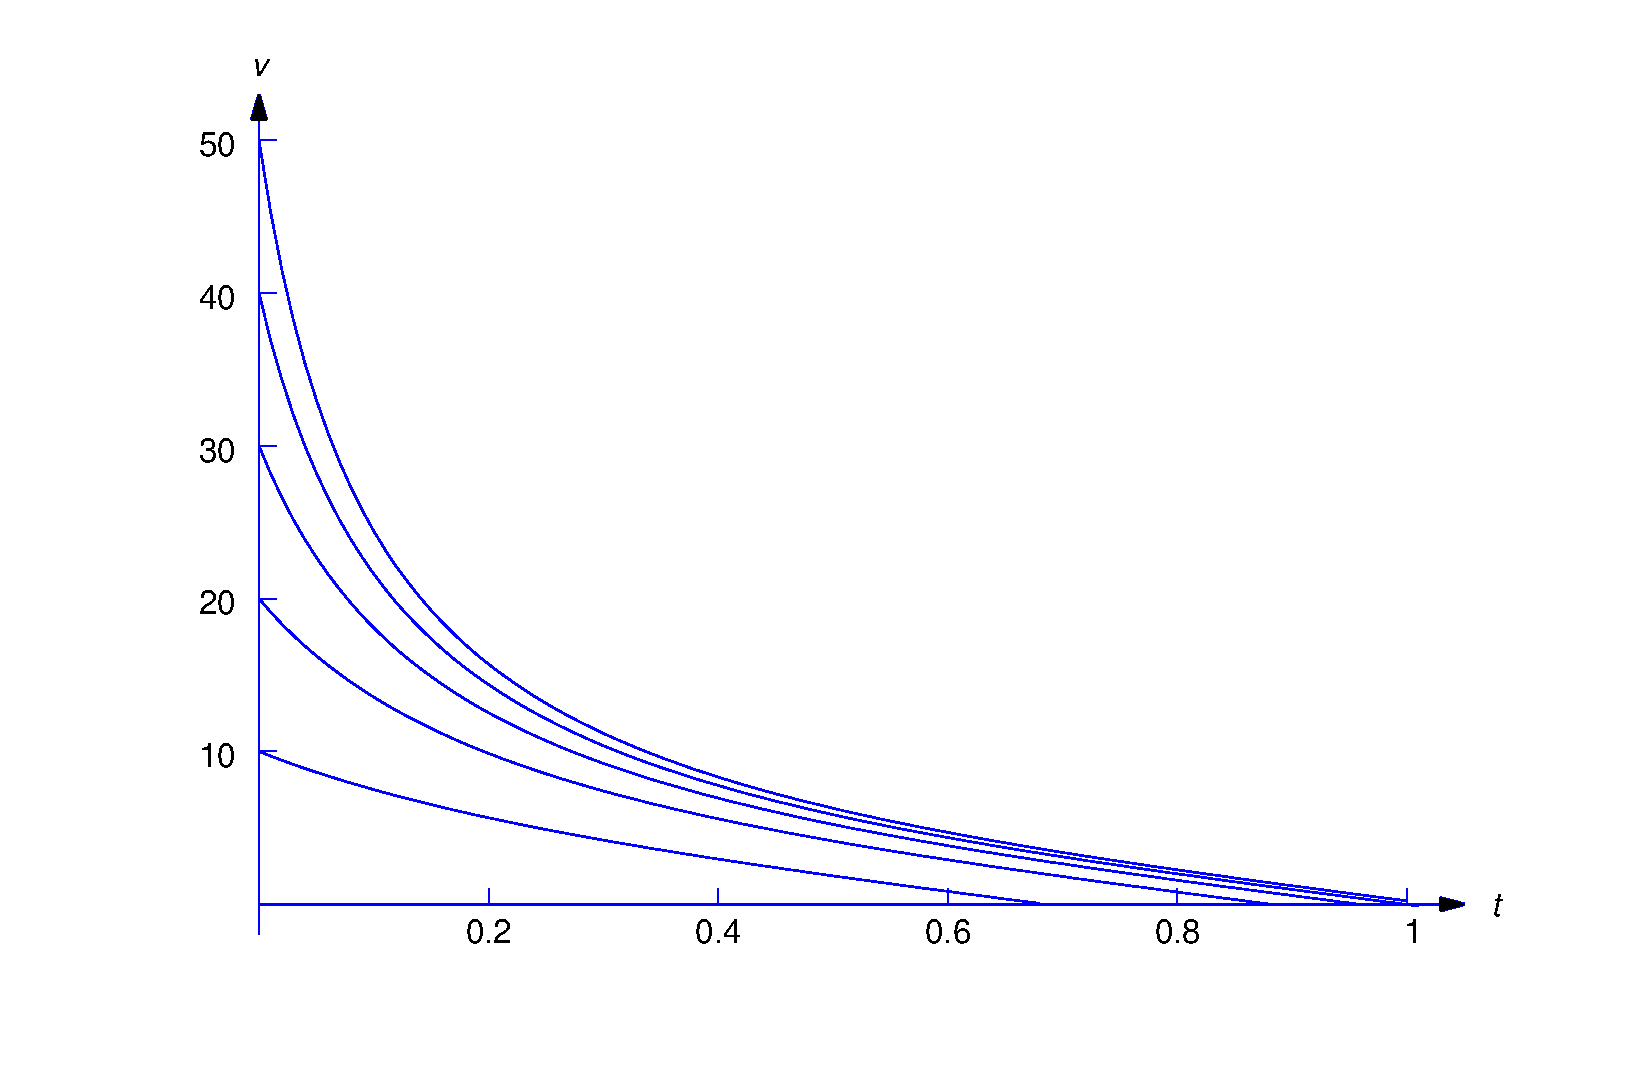
\includegraphics[bb=-78 148 689 643, width=5.67in, height=3.66in, keepaspectratio]{fig040304}
  \relax
  \caption{Solutions of (\ref{eq:4.3.15}) for various $v_{0}>0$}
  \label{figure:4.3.4}
\end{figure}
\end{examplesolution}

\section*{Section 4.4}
\setcounter{chapter}{4}
\setcounter{section}{4}

\setcounter{example}{0}
\setcounter{equation}{8}
\setcounter{figure}{1}
\begin{example}
  $[$The Undamped Spring - Mass System$]\,$\label{example:4.4.1}\rm Consider an object with mass $m$
  suspended from a spring and moving vertically. Let $y$ be the displacement of the object from the
  position it occupies when suspended at rest from the spring (Figure~\ref{figure:4.4.2}).

  \begin{figure}[H]
    \centering
    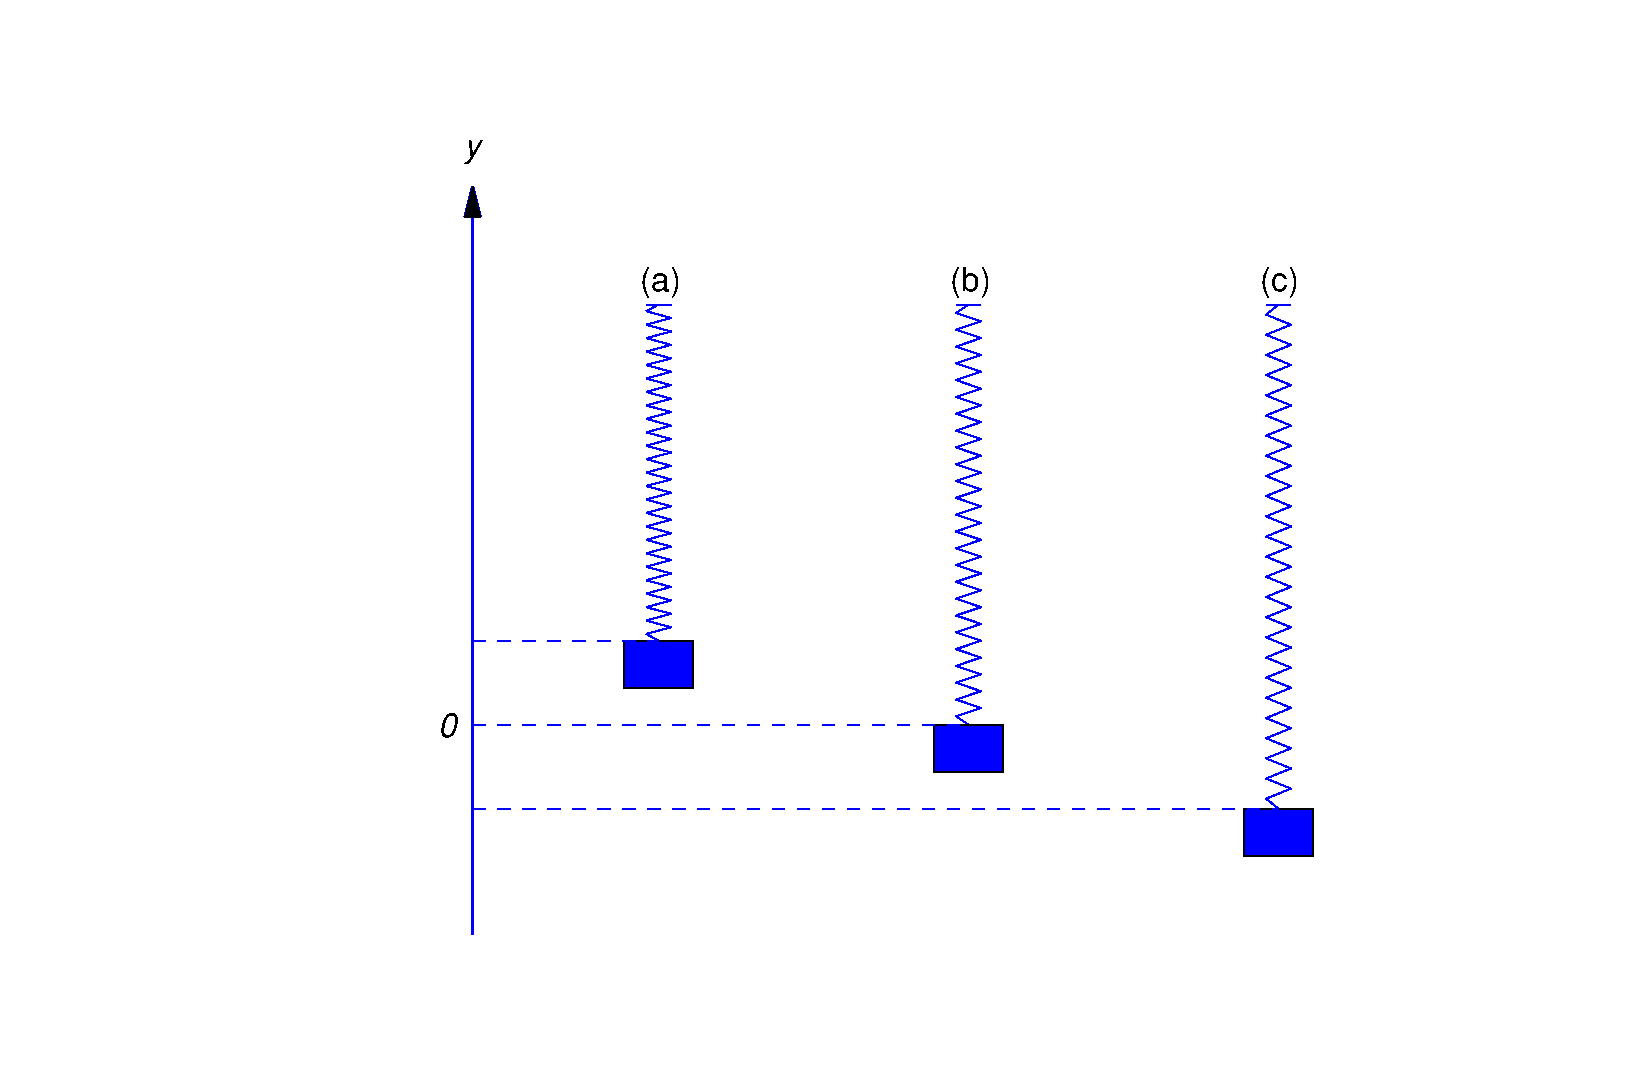
\includegraphics[bb=-78 148 689 643, width=5.67in, height=3.66in, keepaspectratio]{fig040402}
    \relax
    \caption{\,\part{a} $y>0$ \, \part{b} $y=0$ \, \part{c} $y<0$}
    \label{figure:4.4.2}
  \end{figure}

  Assume that if the length of the spring is changed by an amount $\Delta L$ (positive or negative),
  then the spring exerts an opposing force with magnitude $k|\Delta L|$, where $k$ is a positive
  constant. In Section~6.1 it will be shown that if the mass of the spring is negligible compared to
  $m$ and no other forces act on the object then Newton's second law of motion implies that
  \begin{equation}
    \label{eq:4.4.9}my''=-ky,
  \end{equation}
  which can be written in the form \textup{(4.4.7)} with $p(y)=ky/m$. This equation can be solved
  easily by a method that we'll study in Section~5.2, but that method isn't available here. Instead,
  we'll consider the phase plane equivalent of \eqref{eq:4.4.9}.

  From \textup{(4.4.3)}, we can rewrite \eqref{eq:4.4.9} as the separable equation
  \[
    mv\frac{dv}{dy}=-ky.
  \]
  Integrating this yields
  \[
    \frac{mv^{2}}{2}=-\frac{ky^{2}}{2}+c,
  \]
  which implies that
  \begin{equation}
    \label{eq:4.4.10}mv^{2}+ky^{2}=\rho
  \end{equation}
  ($\rho=2c$). This defines an ellipse in the Poincar\'e phase plane (Figure~\ref{figure:4.4.3}).

  \begin{figure}[H]
    \centering
    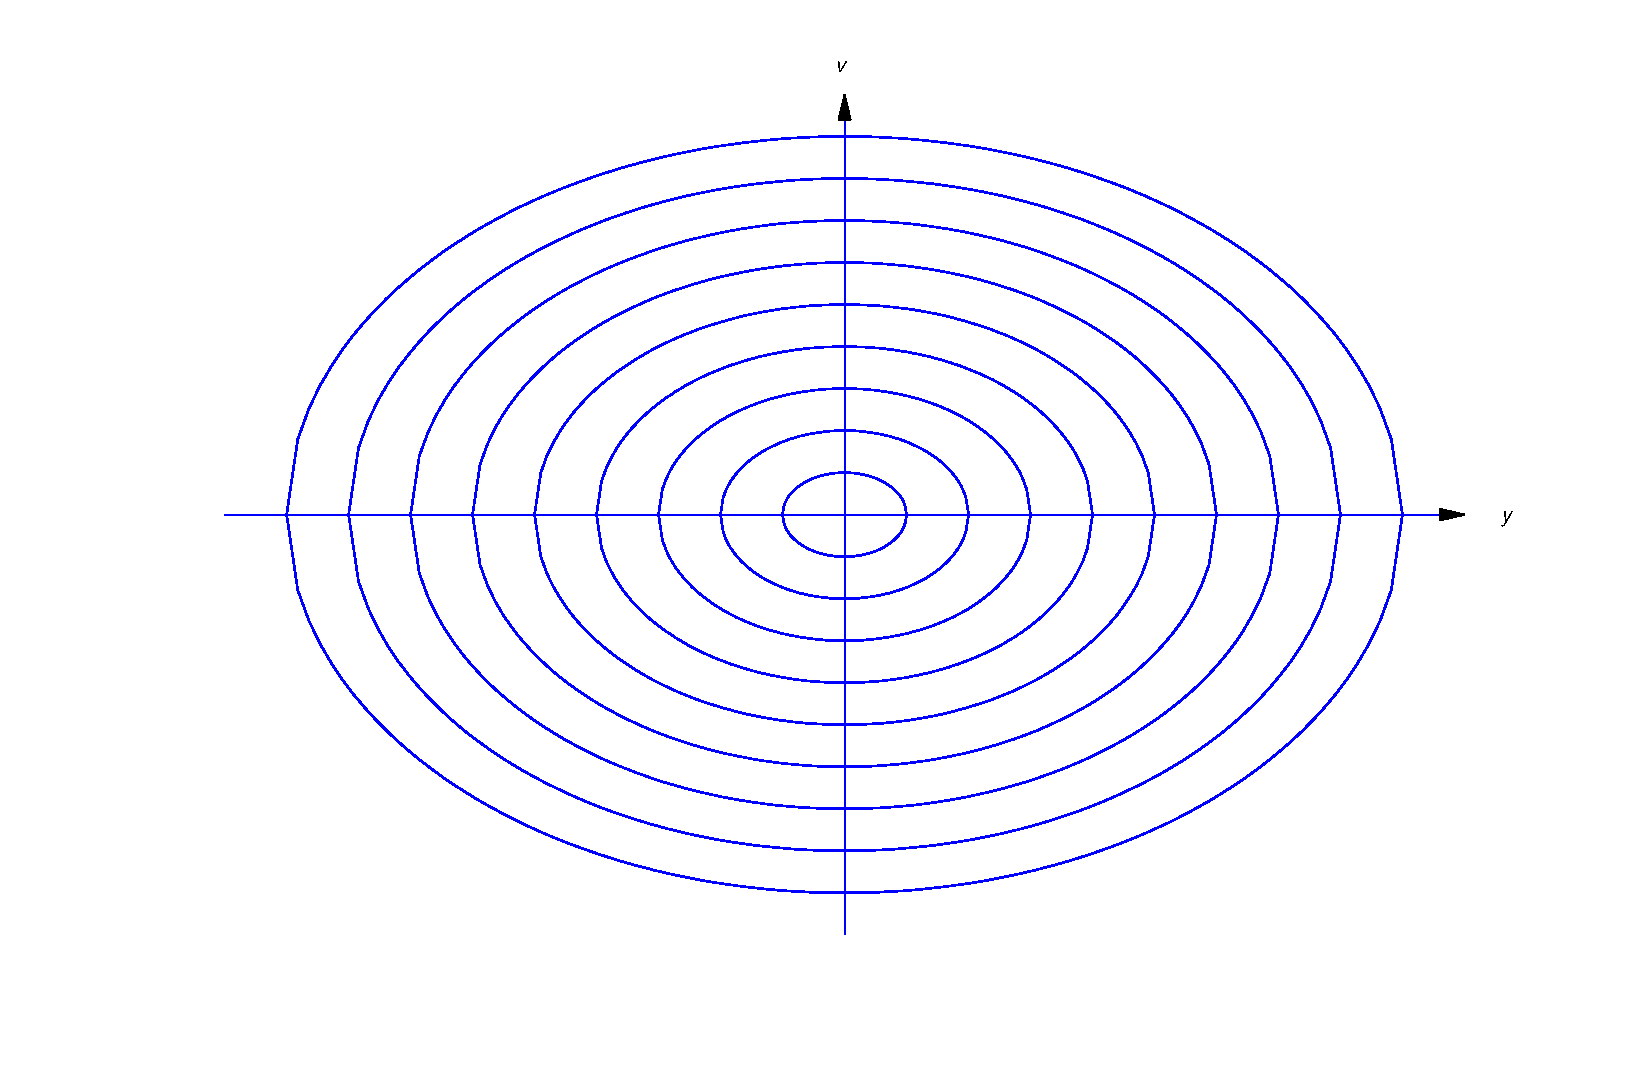
\includegraphics[bb=-78 148 689 643, width=5.67in, height=3.66in, keepaspectratio]{fig040403}
    \relax
    \caption{Trajectories of $my''+ky=0$}
    \label{figure:4.4.3}
  \end{figure}

  We can identify $\rho$ by setting $t=0$ in \eqref{eq:4.4.10}; thus, $\rho=mv_{0}^{2}+ky_{0}^{2}$,
  where $y_{0}=y(0)$ and $v_{0}=v(0)$. To determine the maximum and minimum values of $y$ we set
  $v=0$ in \eqref{eq:4.4.10}; thus,
  \begin{equation}
    \label{eq:4.4.11}y_{\max}=R\mbox{\quad and \quad}y_{\min}=-R,\mbox{\quad with }R=\sqrt{\frac{\rho}{k}}.
  \end{equation}
  Equation~\eqref{eq:4.4.9} has exactly one equilibrium, $\overline{y}=0$, and it's stable. You can
  see intuitively why this is so: if the object is displaced in either direction from equilibrium,
  the spring tries to bring it back.

  In this case we can find $y$ explicitly as a function of $t$. (Don't expect this to happen in more
  complicated problems!) If $v>0$ on an interval $I$, \eqref{eq:4.4.10} implies that
  \[
    \frac{dy}{dt}=v=\sqrt{\frac{\rho-ky^{2}}{m}}
  \]
  on $I$. This is equivalent to
  \begin{equation}
    \label{eq:4.4.12}\frac{\sqrt{k}}{\sqrt{\rho-ky^{2}}}\frac{dy}{dt}=\omega_{0},\mbox{\quad where \quad}\omega_{0}=\sqrt{\frac{k}{m}}.
  \end{equation}
  Since
  \[
    \int\frac{\sqrt{k}\,dy}{\sqrt{\rho-ky^{2}}}=\sin^{-1}\left(\sqrt{\frac{k}{\rho}}y\right)+c=\sin^{-1}\left(\frac{y}{R}\right)+c
  \]
  (see \eqref{eq:4.4.11}), \eqref{eq:4.4.12} implies that there's a constant $\phi$ such that
  \[
    \sin^{-1}\left(\frac{y}{R}\right)=\omega_{0}t+\phi
  \]
  or
  \[
    y=R\sin(\omega_{0}t+\phi)
  \]
  for all $t$ in $I$. Although we obtained this function by assuming that $v>0$, you can easily
  verify that $y$ satisfies \eqref{eq:4.4.9} for all values of $t$. Thus, the displacement varies
  periodically between $-R$ and $R$, with period $T=2\pi/\omega_{0}$ (Figure~4.4.4).
  (If you've taken a course in elementary mechanics you may recognize this as {\relax\it
  simple harmonic motion\/}.)
\end{example}

\setcounter{example}{1}
\setcounter{equation}{12}
\setcounter{figure}{4}
\begin{example}
  $[$The Undamped Pendulum$]$\label{example:4.4.2}\rm \, Now we consider the motion of a pendulum
  with mass $m$, attached to the end of a weightless rod with length $L$ that rotates on a
  frictionless axle (Figure~\ref{figure:4.4.5}). We assume that there's no air resistance.

  Let $y$ be the angle measured from the rest position (vertically downward) of the pendulum, as
  shown in Figure~\ref{figure:4.4.5}. Newton's second law of motion says that the product of $m$ and
  the tangential acceleration equals the tangential component of the gravitational force; therefore,
  from Figure~\ref{figure:4.4.5},
  \[
    mLy''=-mg\sin y,
  \]
  or
  \begin{equation}
    \label{eq:4.4.13}y''=-\frac{g}{L}\sin y.
  \end{equation}

  \begin{figure}[H]
    \centering
    \scalebox{.5}{
    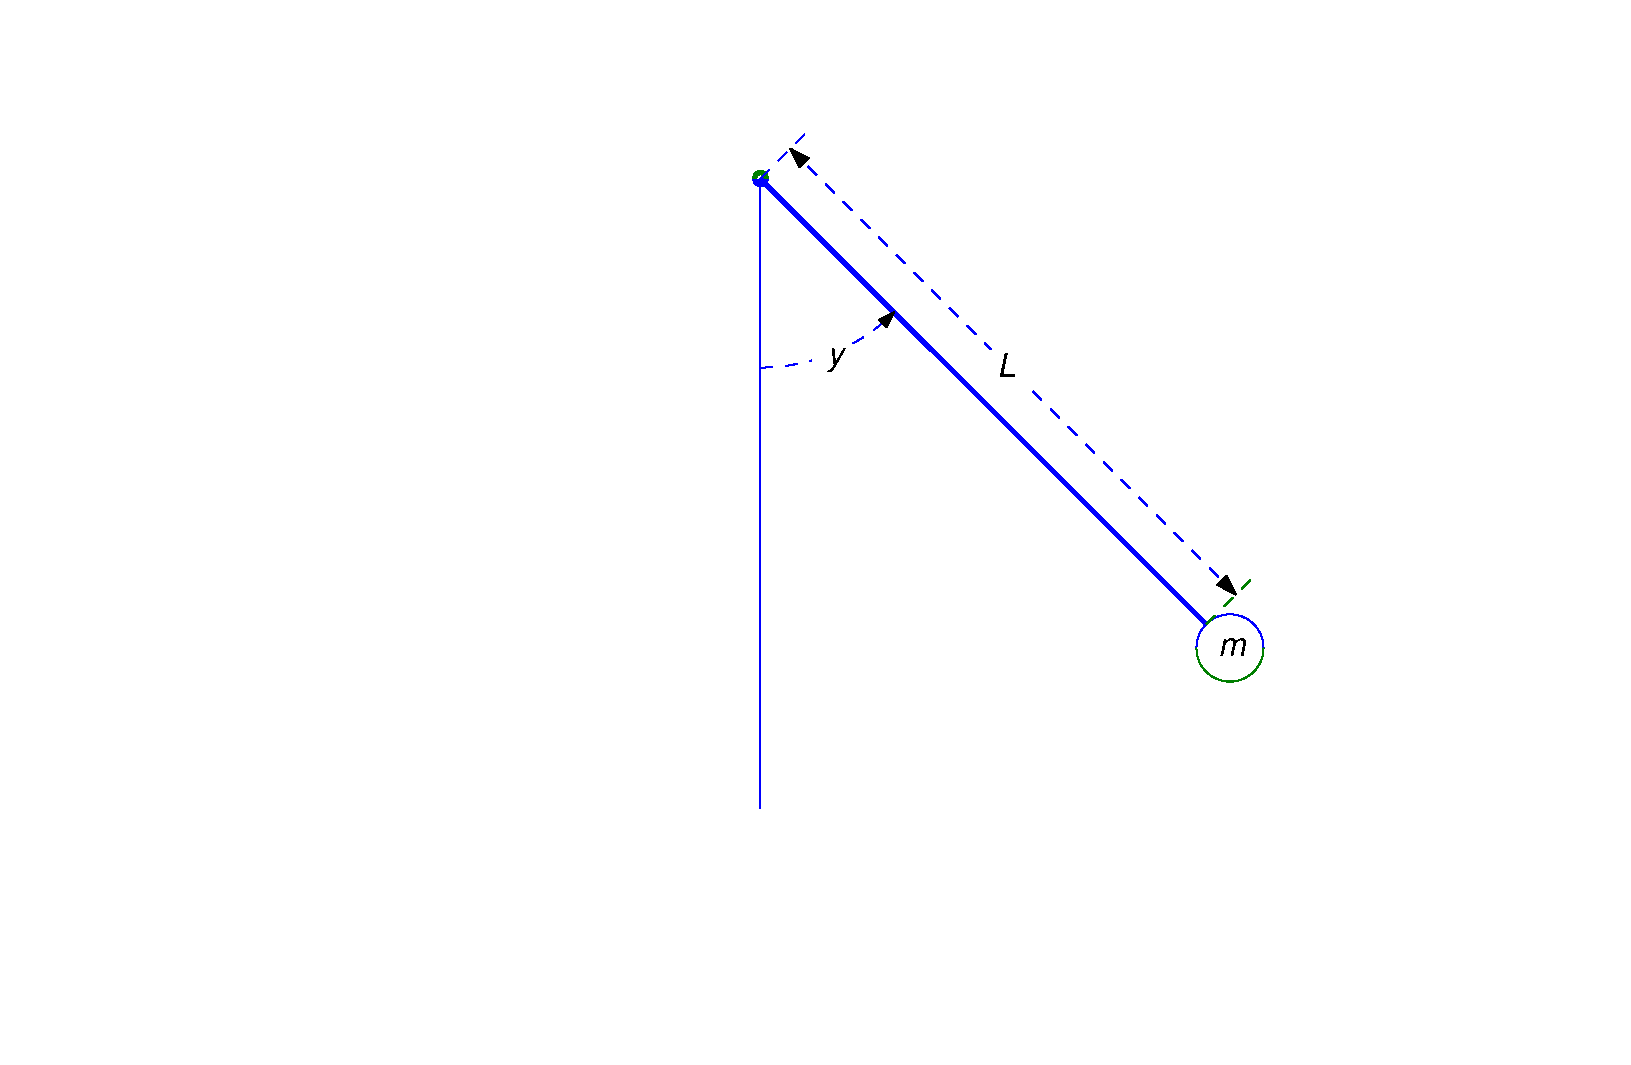
\includegraphics[bb=-78 148 689 643, width=5.67in, height=3.66in, keepaspectratio]{fig040405}
    }
    \relax
    \caption{The undamped pendulum}
    \label{figure:4.4.5}
  \end{figure}

  Since $\sin n\pi=0$ if $n$ is any integer, \eqref{eq:4.4.13} has infinitely many equilibria
  $\overline{y}_{n}=n\pi$. If $n$ is even, the mass is directly below the axle
  (Figure~\ref{figure:4.4.6}~\part{a}) and gravity opposes any deviation from the equilibrium.
  However, if $n$ is odd, the mass is directly above the axle (Figure~\ref{figure:4.4.6}~\part{b})
  and gravity increases any deviation from the equilibrium. Therefore we conclude on physical
  grounds that $\overline{y}_{2m}=2m\pi$ is stable and $\overline{y}_{2m+1}=(2m+1)\pi$ is unstable.

  \begin{figure}[H]
    \centering
    \scalebox{.5}{
    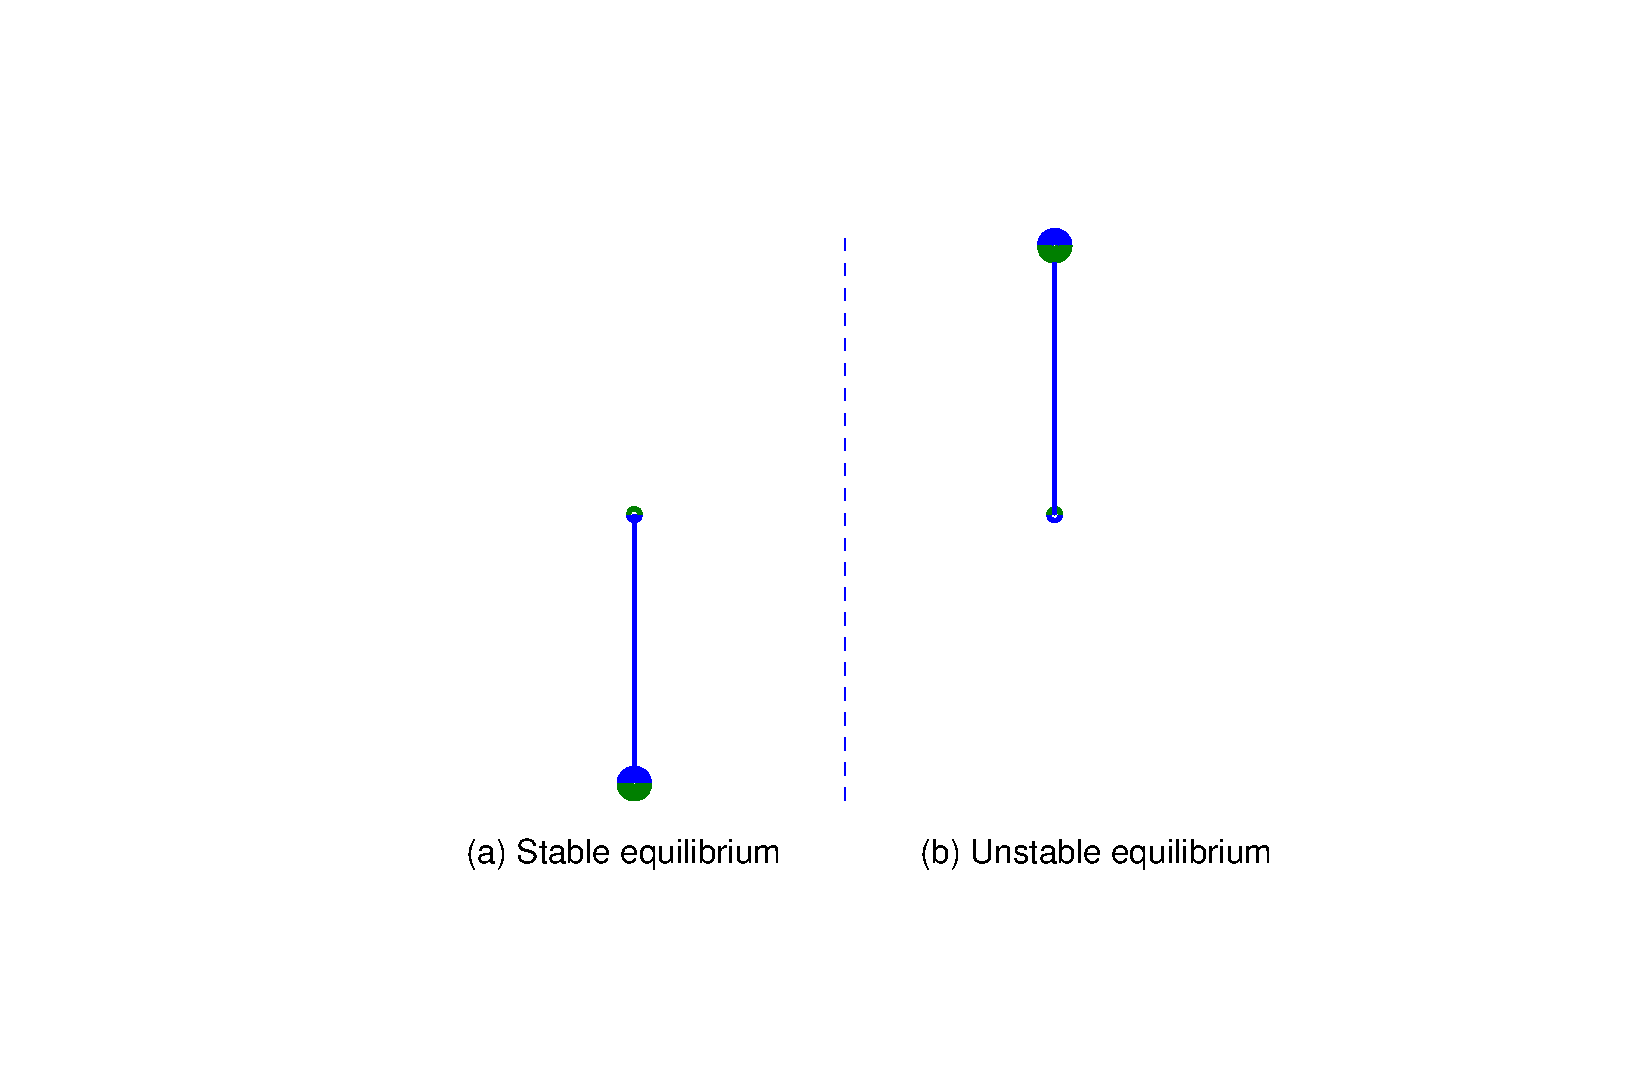
\includegraphics[bb=-78 148 689 643, width=5.67in, height=3.66in, keepaspectratio]{fig040406}
    }
    \relax
    \caption{\part{a}\, Stable equilibrium \, \part{b}\, Unstable equilibrium}
    \label{figure:4.4.6}
  \end{figure}

  The phase plane equivalent of \eqref{eq:4.4.13} is
  \[
    v\frac{dv}{dy}=-\frac{g}{L}\sin y,
  \]
  where $v=y'$ is the angular velocity of the pendulum. Integrating this yields
  \begin{equation}
    \label{eq:4.4.14}\frac{v^{2}}{2}=\frac{g}{L}\cos y+c.
  \end{equation}
  If $v=v_{0}$ when $y=0$, then
  \[
    c=\frac{v_{0}^{2}}{2}-\frac{g}{L},
  \]
  so \eqref{eq:4.4.14} becomes
  \[
    \frac{v^{2}}{2}=\frac{v_{0}^{2}}{2}-\frac{g}{L}(1-\cos y) =\frac{v_{0}^{2}}{2}-\frac{2g}{L}\sin^{2}\frac{y}{2},
  \]
  which is equivalent to
  \begin{equation}
    \label{eq:4.4.15}v^{2}=v_{0}^{2}-v_{c}^{2}\sin^{2}\frac{y}{2},
  \end{equation}
  where
  \[
    v_{c}=2\sqrt{\frac{g}{L}}.
  \]

  The curves defined by \eqref{eq:4.4.15} are the trajectories of \eqref{eq:4.4.13}. They are
  periodic with period $2\pi$ in $y$, which isn't surprising, since if $y=y(t)$ is a solution of
  \eqref{eq:4.4.13} then so is $y_{n}=y(t)+2n\pi$ for any integer $n$. Figure~4.4.7
  shows trajectories over the interval $[-\pi,\pi]$. From \eqref{eq:4.4.15}, you can see that if
  $|v_{0}|>v_{c}$ then $v$ is nonzero for all $t$, which means that the object whirls in the same
  direction forever, as in Figure~4.4.8. The trajectories associated with this whirling
  motion are above the upper dashed curve and below the lower dashed curve in
  Figure~4.4.7. You can also see from \eqref{eq:4.4.15} that if $0<|v_{0}|<v_{c}$,then
  $v=0$ when $y=\pm y_{\max}$, where
  \[
    y_{\max}=2\sin^{-1}(|v_{0}|/v_{c}).
  \]
  In this case the pendulum oscillates periodically between $-y_{\max}$ and $y_{\max}$, as shown in
  Figure~4.4.9. The trajectories associated with this kind of motion are the ovals
  between the dashed curves in Figure~4.4.7. It can be shown (see
  Exercise~4.4.21 for a partial proof) that the period of the oscillation is
  \begin{equation}
    \label{eq:4.4.16}T=8\int_{0}^{\pi/2}\frac{d\theta}{\sqrt{v_{c}^{2}-v_{0}^{2}\sin^{2}\theta}}.
  \end{equation}
  Although this integral can't be evaluated in terms of familiar elementary functions, you can see
  that it's finite if $|v_{0}|<v_{c}$.

  The dashed curves in Figure~4.4.7 contain four trajectories. The critical points
  $(\pi,0)$ and $(-\pi,0)$ are the trajectories of the unstable equilibrium solutions
  $\overline{y}=\pm\pi$. The upper dashed curve connecting (but not including) them is obtained from
  initial conditions of the form $y(t_{0})=0$, $v(t_{0})=v_{c}$. If $y$ is any solution with this
  trajectory then
  \[
    \lim_{t\to\infty}y(t)=\pi\mbox{\quad and \quad}\lim_{t\to-\infty}y(t)=-\pi.
  \]
  The lower dashed curve connecting (but not including) them is obtained from initial conditions of
  the form $y(t_{0})=0$, $v(t_{0})=-v_{c}$. If $y$ is any solution with this trajectory then
  \[
    \lim_{t\to\infty}y(t)=-\pi\mbox{\quad and \quad}\lim_{t\to-\infty}y(t)=\pi.
  \]
  Consistent with this, the integral \eqref{eq:4.4.16} diverges to $\infty$ if $v_{0}=\pm v_{c}$.
  (Exercise~4.4.21) .

  Since the dashed curves separate trajectories of whirling solutions from trajectories of
  oscillating solutions, each of these curves is called a {\relax\it separatrix\/}.

  In general, if \textup{(4.4.7)} has both stable and unstable equilibria then the separatrices are
  the curves given by \textup{(4.4.8)} that pass through unstable critical points. Thus, if
  $(\overline{y},0)$ is an unstable critical point, then
  \begin{equation}
    \label{eq:4.4.17}\frac{v^{2}}{2}+P(y)=P(\overline{y})
  \end{equation}
  \enlargethispage{30pt}
  defines a separatrix passing through $(\overline{y},0)$.
\end{example}

\setcounter{example}{2}
\setcounter{equation}{21}
\setcounter{figure}{9}
\begin{example}
  \label{example:4.4.3}\rm The equation
  \begin{equation}
    \label{eq:4.4.22}y''+y(y-1)=0
  \end{equation}
  is of the form \textup{(4.4.18)} with $p(y)=y(y-1)$. Therefore $\overline{y}=0$ and
  $\overline{y}=1$ are the equilibria of \eqref{eq:4.4.22}. Since
  \begin{eqnarray*}
    y(y-1)>0 & \text{\, if \,}y<0\mbox{\, or \,}y>1, \\
    <0       & \hspace*{-22pt}\text{\, if \,}0<y<1,
  \end{eqnarray*}
  $\overline{y}=0$ is unstable and $\overline{y}=1$ is stable.

  The phase plane equivalent of \eqref{eq:4.4.22} is the separable equation
  \[
    v\frac{dv}{dy}+y(y-1)=0.
  \]
  Integrating yields
  \[
    \frac{v^{2}}{2}+\frac{y^{3}}{3}-\frac{y^{2}}{2}=C,
  \]
  which we rewrite as
  \begin{equation}
    \label{eq:4.4.23}v^{2}+\frac{1}{3}y^{2}(2y-3)=c
  \end{equation}
  after renaming the constant of integration. These are the trajectories of \eqref{eq:4.4.22}. If
  $y$ is any solution of \eqref{eq:4.4.22}, the point $(y(t),v(t))$ moves along the trajectory of
  $y$ in the direction of increasing $y$ in the upper half plane ($v=y'>0$), or in the direction of
  decreasing $y$ in the lower half plane ($v=y'<0$).

  Figure~\ref{figure:4.4.10} shows typical trajectories. The dashed curve through the critical point
  $(0,0)$, obtained by setting $c=0$ in \eqref{eq:4.4.23}, separates the $y$-$v$ plane into regions
  that contain different kinds of trajectories; again, we call this curve a {\relax\it
  separatrix\/}. Trajectories in the region bounded by the closed loop \part{b} are closed curves,
  so solutions associated with them are periodic. Solutions associated with other trajectories are
  not periodic. If $y$ is any such solution with trajectory not on the separatrix, let $(t_{-},t_{+})$ be its maximal interval of existence. Both endpoints are finite, and then
  \[
    \begin{array}{llrllr}
      \dst\lim_{t\to t_{+}}y(t) & = & -\infty, & \dst\lim_{t\to t_{-}}y(t) & = & -\infty, \\
      \dst\lim_{t\to t_{+}}v(t) & = & -\infty, & \dst\lim_{t\to t_{-}}v(t) & = & \infty.
    \end{array}
  \]

  \begin{figure}[H]
    \centering
    \relax
    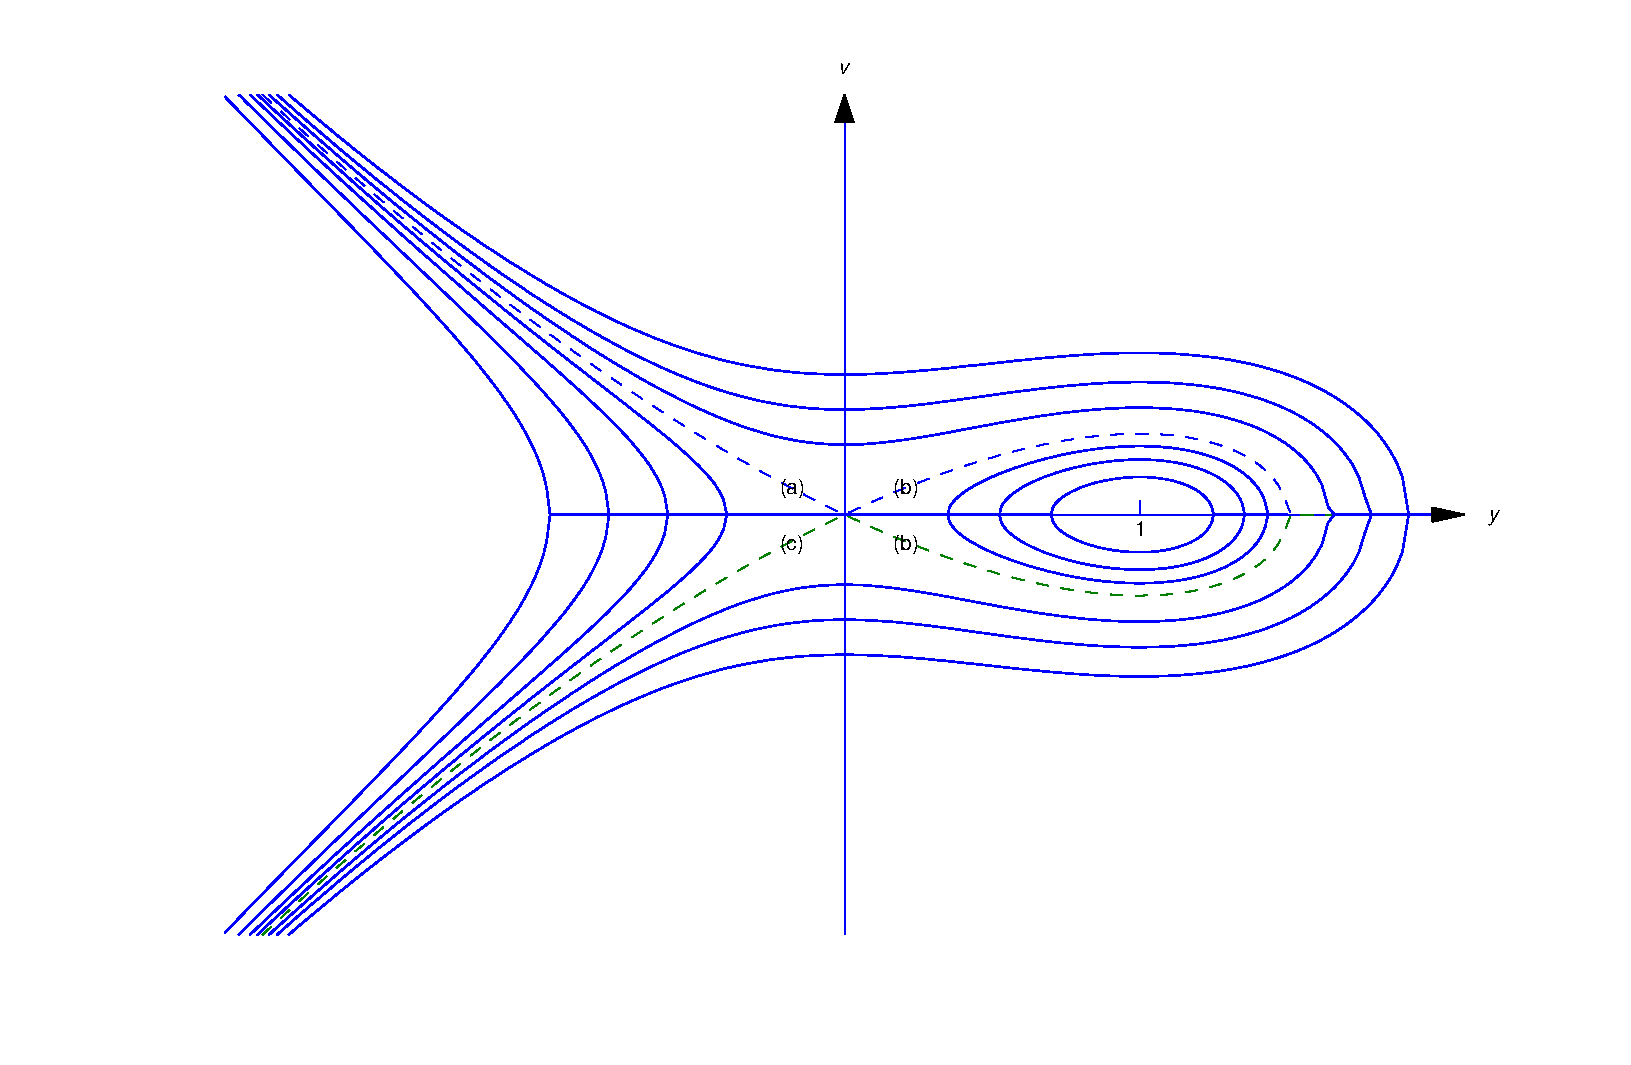
\includegraphics[bb=-78 148 689 643, width=5.67in, height=3.66in, keepaspectratio]{fig040410}
    \caption{Trajectories of $y''+y(y-1)=0$}
    \label{figure:4.4.10}
  \end{figure}

  The separatrix contains four trajectories of \eqref{eq:4.4.22}. One is the point $(0,0)$, the
  trajectory of the equilibrium $\overline{y}=0$. Since distinct trajectories can't intersect, the
  segments of the separatrix marked \part{a}, \part{b}, and \part{c} -- which don't include $(0,0)$
  -- are distinct trajectories, none of which can be traversed in finite time. For each solution, let $(t_{-},t_{+})$ be its maximal interval of existence. On \part{a} and \part{c}, the endpoint at which $y$ tends to $-\infty$ is finite. Solutions with these
  trajectories have the following asymptotic behavior:
  \[
    \begin{array}{llrllrl}
      \dst\lim_{t\to\infty}y(t) & = & 0,       & \dst\lim_{t\to t_{-}}y(t) & = & -\infty,           \\
      \dst\lim_{t\to\infty}v(t) & = & 0,       & \dst\lim_{t\to t_{-}}v(t) & = & \infty\phantom{,} & \mbox{ (on \part{a})}  \\
      \dst\lim_{t\to\infty}y(t) & = & 0,       & \dst\lim_{t\to-\infty}y(t) & = & 0,                 \\
      \dst\lim_{t\to\infty}v(t) & = & 0,       & \dst\lim_{t\to-\infty}v(t) & = & 0\phantom{,}      & \mbox{ (on \part{b})}  \\
      \dst\lim_{t\to t_{+}}y(t) & = & -\infty, & \dst\lim_{t\to-\infty}y(t) & = & 0,                 \\
      \dst\lim_{t\to t_{+}}v(t) & = & -\infty, & \dst\lim_{t\to-\infty}v(t) & = & 0\phantom{,}      & \mbox{ (on \part{c})}.
    \end{array}.
  \]
\end{example}

\setcounter{example}{3}
\setcounter{equation}{28}
\begin{example}[The Damped Pendulum]
  \label{example:4.4.5} \rm Now we return to the pendulum. If we assume that some mechanism (for
  example, friction in the axle or atmospheric resistance) opposes the motion of the pendulum with a
  force proportional to its angular velocity, Newton's second law of motion implies that
  \begin{equation}
    \label{eq:4.4.29}mLy''=-cy'-mg\sin y,
  \end{equation}
  where $c>0$ is the damping constant. (Again, a minor note: the $c$ in \textup{(4.4.26)} actually
  corresponds to $c/mL$ in this equation.) To plot a direction field for \eqref{eq:4.4.29} we write
  its phase plane equivalent as
  \[
    \frac{dv}{dy}=-\frac{c}{mL}-\frac{g}{Lv}\sin y.
  \]
  Figure~4.4.15 shows trajectories of four solutions of \eqref{eq:4.4.29}, all
  satisfying $y(0)=0$. For each $m=0$, $1$, $2$, $3$, imparting the initial velocity $v(0)=v_{m}$
  causes the pendulum to make $m$ complete revolutions and then settle into decaying oscillation
  about the stable equilibrium $\overline{y}=2m\pi$.
\end{example}

\section*{Section 4.5}
\setcounter{chapter}{4}
\setcounter{section}{5}

\setcounter{example}{0}
\setcounter{equation}{0}
\begin{example}
  \label{example:4.5.1} \rm For each value of the parameter $c$, the equation
  \begin{equation}
    \label{eq:4.5.1}y-cx^{2}=0
  \end{equation}
  defines a curve in the $xy$-plane. If $c\ne0$, the curve is a parabola through the origin, opening
  upward if $c>0$ or downward if $c<0$. If $c=0$, the curve is the $x$ axis
  (Figure~4.5.1).
\end{example}

\setcounter{example}{1}
\setcounter{equation}{1}
\begin{example}
  \label{example:4.5.2} \rm For each value of the parameter $c$ the equation
  \begin{equation}
    \label{eq:4.5.2}y=x+c
  \end{equation}
  defines a line with slope 1(Figure~4.5.2).
\end{example}

\setcounter{example}{2}
\setcounter{equation}{3}
\begin{example}
  \label{example:4.5.3} \rm If $c>0$, the graph of the equation
  \begin{equation}
    \label{eq:4.5.4}x^{2}+y^{2}-c=0
  \end{equation}
  is a circle with center at $(0,0)$ and radius $\sqrt{c}$. If $c=0$, the graph is the single point
  $(0,0)$. (We don't regard a single point as a curve.) If $c<0$, the equation has no graph. Hence,
  \eqref{eq:4.5.4} defines a one--parameter family of curves for positive values of $c$. This family
  consists of all circles centered at $(0,0)$ (Figure~4.5.3).
\end{example}

\setcounter{example}{3}
\begin{example}
  \label{example:4.5.4} \rm The equation
  \[
    x^{2}+y^{2}+c^{2}=0
  \]
  does not define a one-parameter family of curves, since no $(x,y)$ satisfies the equation if
  $c\ne0$, and only the single point $(0,0)$ satisfies it if $c=0$. \bbox
\end{example}

\setcounter{example}{4}
\setcounter{equation}{7}
\begin{example}
  \label{example:4.5.5} \rm Find a differential equation for the family of curves defined by
  \begin{equation}
    \label{eq:4.5.8}y=cx^{2}.
  \end{equation}
\end{example}
\begin{examplesolution}
\solution Differentiating \eqref{eq:4.5.8} with respect to $x$ yields
\[
  y'=2cx.
\]
Therefore $c=y'/2x$, and substituting this into \eqref{eq:4.5.8} yields
\[
  y=\frac{xy'}{2}
\]
as a differential equation for the family of curves defined by \eqref{eq:4.5.8}. The graph of any
function of the form $y=cx^{2}$ is an integral curve of this equation. \bbox
\end{examplesolution}

\setcounter{example}{5}
\begin{example}
  \label{example:4.5.6} \rm \mbox{}
  \begin{alist}
    \item % (a)
    Try to find a differential equation for the family of lines tangent to the parabola $y=x^{2}$.

    \item % (b)
    Find two tangent lines to the parabola $y=x^{2}$ that pass through $(2,3)$, and find the points
    of tangency.
  \end{alist}
\end{example}
\setcounter{equation}{8}
\setcounter{figure}{3}
\begin{examplesolution}
\solutionpart{a} The equation of the line through a given point $(x_{0},y_{0})$ with slope $m$ is
\begin{equation}
  \label{eq:4.5.9}y=y_{0}+m(x-x_{0}).
\end{equation}
If $(x_{0},y_{0})$ is on the parabola, then $y_{0}=x_{0}^{2}$ and the slope of the tangent line
through $(x_{0},x_{0}^{2})$ is $m=2x_{0}$; hence, \eqref{eq:4.5.9} becomes
\[
  y=x_{0}^{2}+2x_{0}(x-x_{0}),
\]
or, equivalently,
\begin{equation}
  \label{eq:4.5.10}y=-x_{0}^{2}+2x_{0}x.
\end{equation}
Here $x_{0}$ plays the role of the constant $c$ in Definition~4.5.1; that is, varying
$x_{0}$ over $(-\infty,\infty)$ produces the family of tangent lines to the parabola $y=x^{2}$.

Differentiating \eqref{eq:4.5.10} with respect to $x$ yields $y'=2x_{0}$. We can express $x_{0}$ in
terms of $x$ and $y$ by rewriting \eqref{eq:4.5.10} as
\[
  x_{0}^{2}-2x_{0}x+y=0
\]
and using the quadratic formula to obtain
\begin{equation}
  \label{eq:4.5.11}x_{0}=x\pm\sqrt{x^{2}-y}.
\end{equation}
We must choose the plus sign in \eqref{eq:4.5.11} if $x<x_{0}$ and the minus sign if $x>x_{0}$;
thus,
\[
  x_{0}=\left(x+\sqrt{x^{2}-y}\right)\mbox{\, if \,}x<x_{0}
\]
and
\[
  x_{0}=\left(x-\sqrt{x^{2}-y}\right)\mbox{\, if \,}x>x_{0}.
\]
Since $y'=2x_{0}$, this implies that
\begin{equation}
  \label{eq:4.5.12}y'=2\left(x+\sqrt{x^{2}-y}\right),\mbox{\quad if \quad}x<x_{0}
\end{equation}
and
\begin{equation}
  \label{eq:4.5.13}y'=2\left(x-\sqrt{x^{2}-y}\right),\mbox{\quad if \quad}x>x_{0}.
\end{equation}
Neither \eqref{eq:4.5.12} nor \eqref{eq:4.5.13} is a differential equation for the family of tangent
lines to the parabola $y=x^{2}$. However, if each tangent line is regarded as consisting of two
{\relax\it tangent half lines\/} joined at the point of tangency, \eqref{eq:4.5.12} is a
differential equation for the family of tangent half lines on which $x$ is less than the abscissa of
the point of tangency (Figure~\ref{figure:4.5.4}\part{a}), while \eqref{eq:4.5.13} is a differential
equation for the family of tangent half lines on which $x$ is greater than this abscissa
(Figure~\ref{figure:4.5.4}(b)). The parabola $y=x^{2}$ is also an integral curve of both
\eqref{eq:4.5.12} and \eqref{eq:4.5.13}.

\begin{figure}[H]
  \centering
  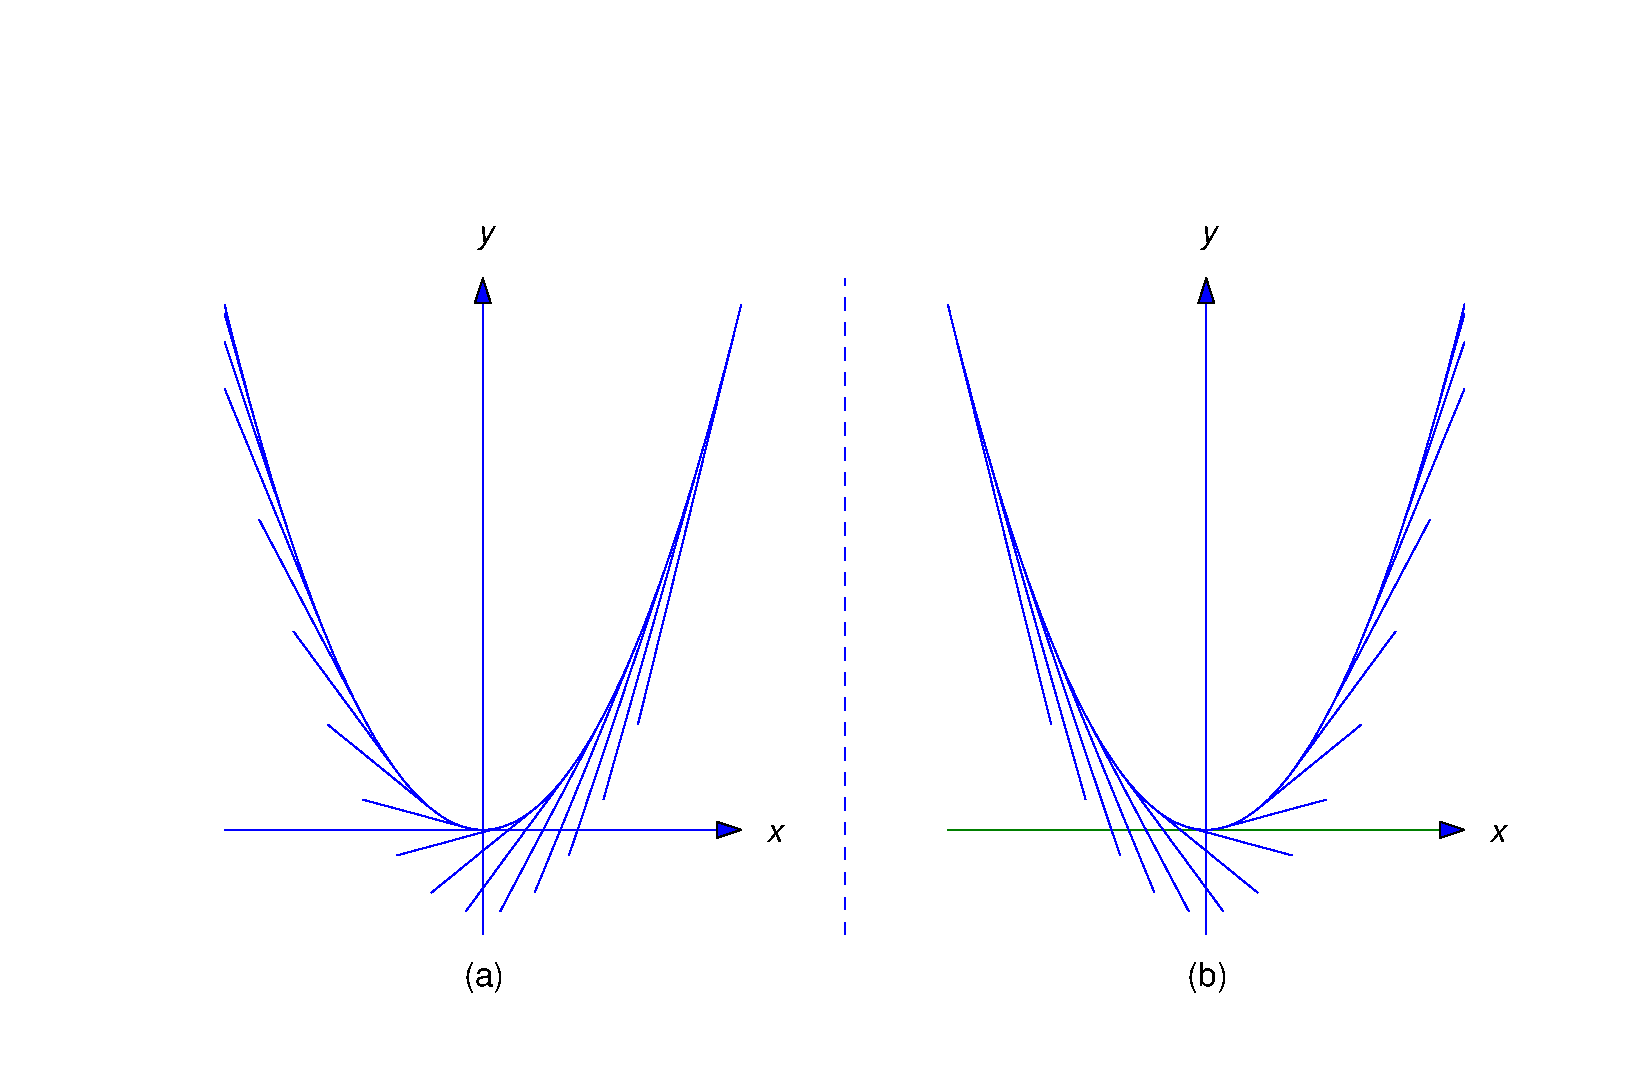
\includegraphics[bb=-78 148 689 643, width=5.67in, height=3.66in, keepaspectratio]{fig040504}
  \relax
  \caption{}
  \label{figure:4.5.4}
\end{figure}

\solutionpart{b} From \eqref{eq:4.5.10} the point $(x,y)=(2,3)$ is on the tangent line through
$(x_{0},x_{0}^{2})$ if and only if
\[
  3=-x_{0}^{2}+4x_{0},
\]
which is equivalent to
\[
  x_{0}^{2}-4x_{0}+3=(x_{0}-3)(x_{0}-1)=0.
\]
Letting $x_{0}=3$ in \eqref{eq:4.5.10} shows that $(2,3)$ is on the line
\[
  y=-9+6x,
\]
which is tangent to the parabola at $(x_{0},x_{0}^{2})=(3,9)$, as shown in Figure~\ref{figure:4.5.5}

Letting $x_{0}=1$ in \eqref{eq:4.5.10} shows that $(2,3)$ is on the line
\[
  y=-1+2x,
\]
which is tangent to the parabola at $(x_{0},x_{0}^{2})=(1,1)$, as shown in
Figure~\ref{figure:4.5.5}.

\vspace*{-15pt}
\begin{figure}[H]
  \centering
  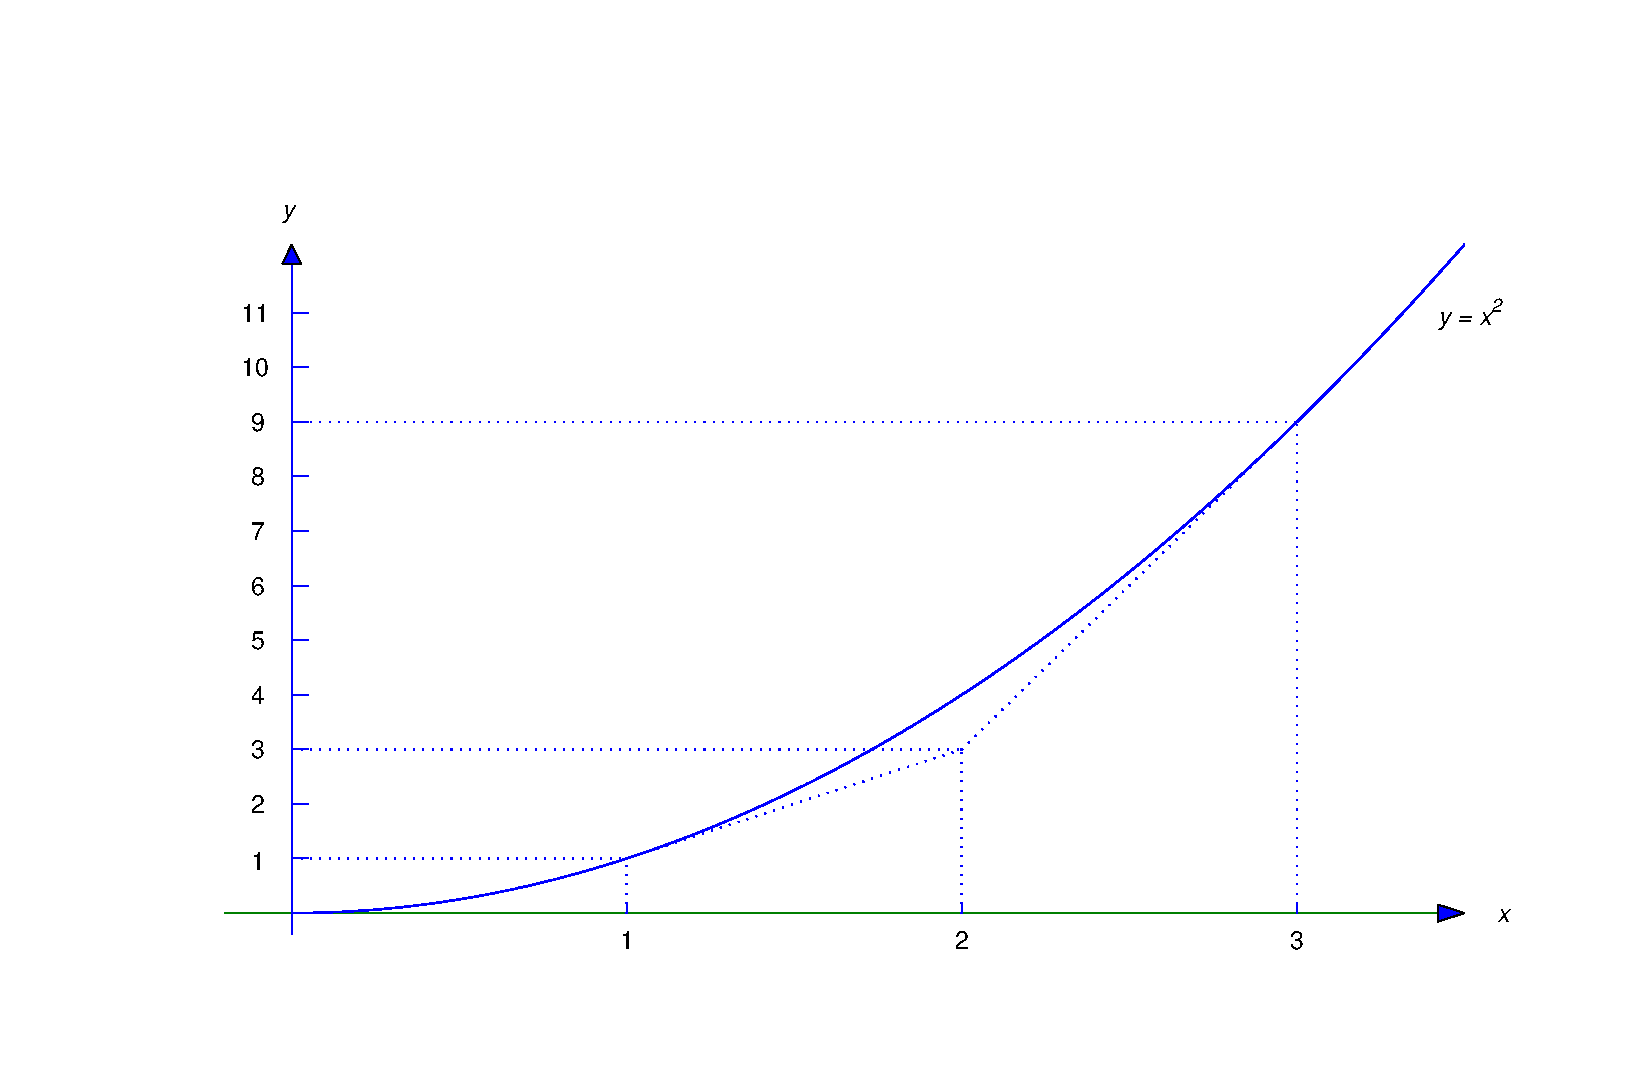
\includegraphics[bb=-78 148 689 643, width=5.67in, height=3.66in, keepaspectratio]{fig040505}
  \caption{}
  \label{figure:4.5.5}
\end{figure}
\end{examplesolution}

\setcounter{example}{6}
\begin{example}
  \label{example:4.5.7} \rm Find curves $y=y(x)$ such that every point $(x_{0},y(x_{0}))$ on the
  curve is the midpoint of the line segment with endpoints on the coordinate axes and tangent to the
  curve at $(x_{0},y(x_{0}))$ (Figure~\ref{figure:4.5.6}).
\end{example}
\setcounter{equation}{13}
\setcounter{figure}{5}
\begin{examplesolution}
\solution The equation of the line tangent to the curve at $P=(x_{0},y(x_{0})$ is
\[
  y=y(x_{0})+y'(x_{0})(x-x_{0}).
\]
If we denote the $x$ and $y$ intercepts of the tangent line by $x_{I}$ and $y_{I}$
(Figure~\ref{figure:4.5.6}), then
\begin{equation}
  \label{eq:4.5.14}0=y(x_{0})+y'(x_{0})(x_{I}-x_{0})
\end{equation}
and
\begin{equation}
  \label{eq:4.5.15}y_{I}=y(x_{0})-y'(x_{0})x_{0}.
\end{equation}
From Figure~\ref{figure:4.5.6}, $P$ is the midpoint of the line segment connecting $(x_{I},0)$ and
$(0,y_{I})$ if and only if $x_{I}=2x_{0}$ and $y_{I}=2y(x_{0})$. Substituting the first of these
conditions into \eqref{eq:4.5.14} or the second into \eqref{eq:4.5.15} yields
\[
  y(x_{0})+y'(x_{0})x_{0}=0.
\]
Since $x_{0}$ is arbitrary we drop the subscript and conclude that $y=y(x)$ satisfies
\[
  y+xy'=0,
\]
which can be rewritten as
\[
  (xy)'=0.
\]
Integrating yields $xy=c$, or
\[
  y=\frac{c}{x}.
\]
If $c=0$ this curve is the line $y=0$, which does not satisfy the geometric requirements imposed by
the problem; thus, $c\ne0$, and the solutions define a family of hyperbolas
(Figure~\ref{figure:4.5.7}).

\begin{figure}[H]
  \relax
  \begin{minipage}[b]{0.5\linewidth}
    \centering
    \scalebox{.65}{
    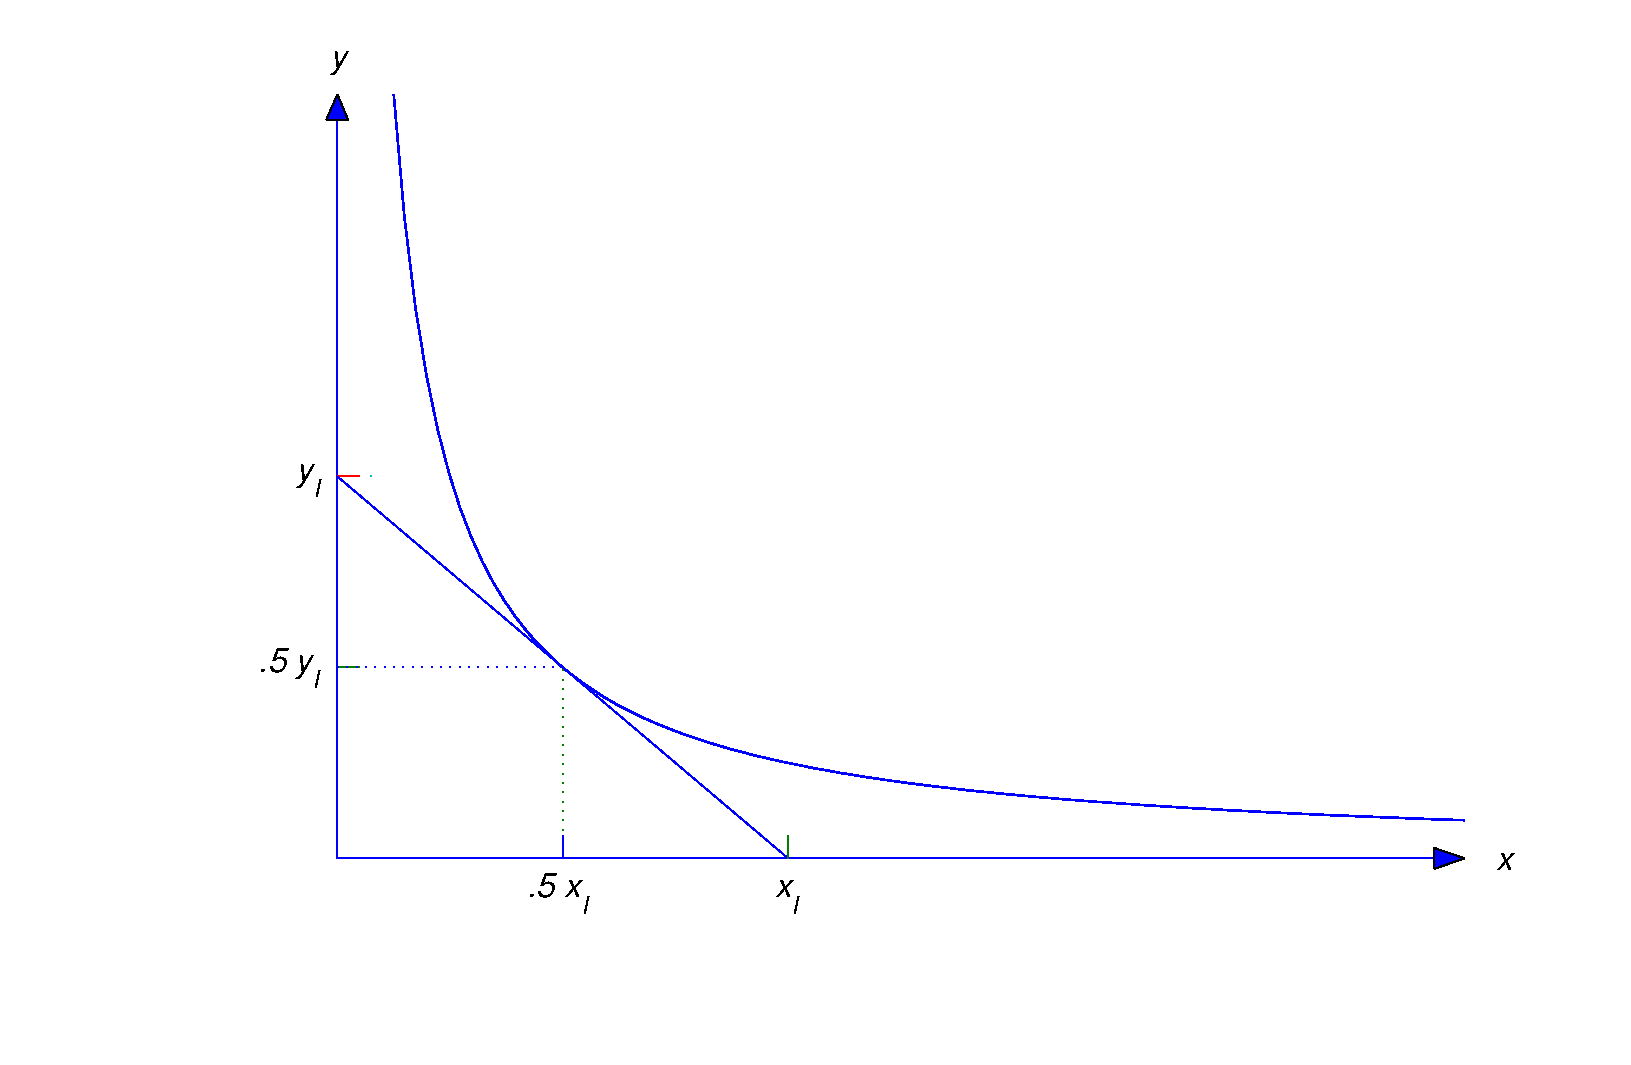
\includegraphics[bb=-78 148 689 643, width=5.67in, height=3.66in, keepaspectratio]{fig040506}
    }
    \caption{}
    \label{figure:4.5.6}
  \end{minipage}
  \hspace{0.6cm}
  \begin{minipage}[b]{0.5\linewidth}
    \centering
    \scalebox{.65}{
    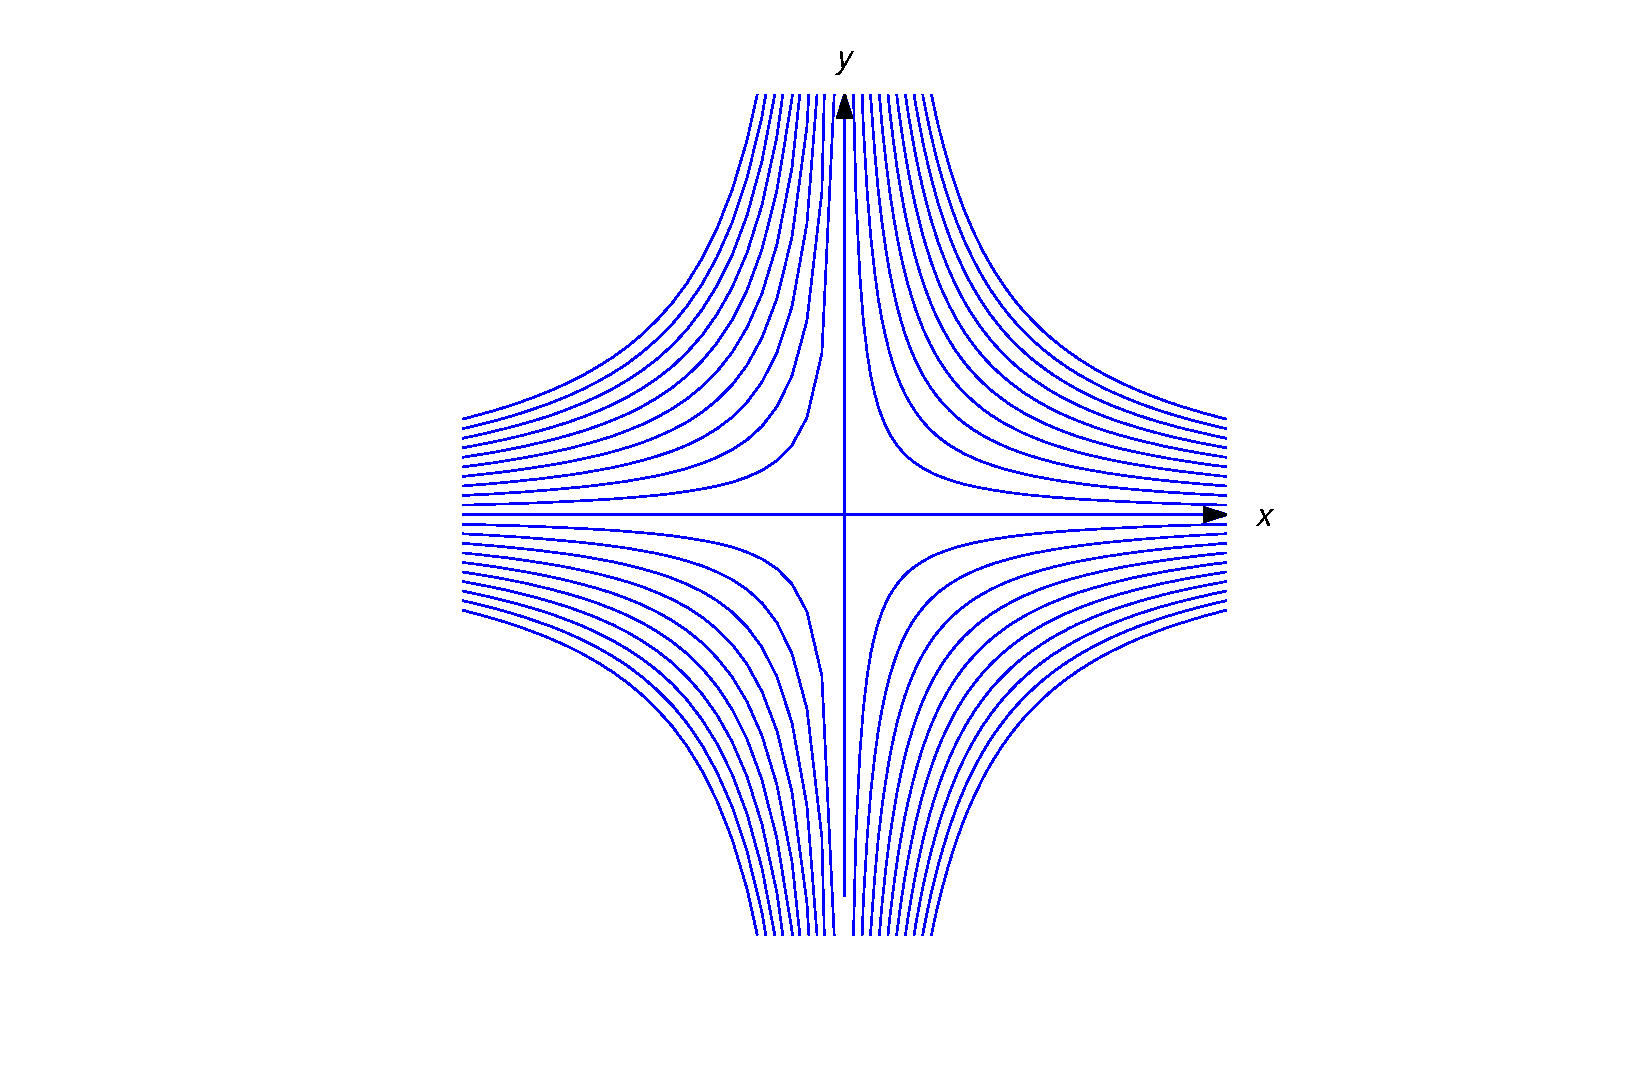
\includegraphics[bb=-78 148 689 643, width=5.67in, height=3.66in, keepaspectratio]{fig040507}}
    \caption{}
    \label{figure:4.5.7}
  \end{minipage}
\end{figure}
\end{examplesolution}

\setcounter{example}{7}
\begin{example}
  \label{example:4.5.8}\rm Find curves $y=y(x)$ such that the tangent line to the curve at any point
  $(x_{0},y(x_{0}))$ intersects the $x$-axis at $(x^{2}_{0},0)$. Figure~4.5.8
  illustrates the situation in the case where the curve is in the first quadrant and $0<x<1$.
\end{example}
\begin{examplesolution}
\solution The equation of the line tangent to the curve at $(x_{0},y(x_{0}))$ is
\[
  y=y(x_{0})+y'(x_{0})(x-x_{0}).
\]
Since $(x^{2}_{0},0)$ is on the tangent line,
\[
  0=y(x_{0})+y'(x_{0})(x^{2}_{0}-x_{0}).
\]
Since $x_{0}$ is arbitrary we drop the subscript and conclude that $y=y(x)$ satisfies
\[
  y+y'(x^{2}-x)=0.
\]
Therefore
\[
  \frac{y'}{y}=-\frac{1}{x^{2}-x}=-\frac{1}{x(x-1)}=\frac{1}{x}-\frac{1}{x-1},
\]
so
\[
  \ln|y|=\ln|x|-\ln|x-1|+k= \ln\left|\frac{x}{x-1}\right|+k,
\]
and
\[
  y=\frac{cx}{x-1}.
\]
If $c=0$, the graph of this function is the $x$-axis. If $c\ne0$, it's a hyperbola with vertical
asymptote $x=1$ and horizontal asymptote $y=c$. Figure~4.5.9 shows the graphs for
$c\ne0$.
\end{examplesolution}

\setcounter{example}{8}
\setcounter{equation}{16}
\begin{example}
  \label{example:4.5.9} \rm Find the orthogonal trajectories of the family of circles
  \begin{equation}
    \label{eq:4.5.17}x^{2}+y^{2}=c^{2}\quad(c>0).
  \end{equation}
\end{example}
\begin{examplesolution}
\solution To find a differential equation for the family of circles we differentiate
\eqref{eq:4.5.17} implicitly with respect to $x$ to obtain
\[
  2x+2yy'=0,
\]
or
\[
  y'=-\frac{x}{y}.
\]
Therefore the integral curves of
\[
  y'=\frac{y}{x}
\]
are orthogonal trajectories of the given family. We leave it to you to verify that the general
solution of this equation is
\[
  y=kx,
\]
where $k$ is an arbitrary constant. This is the equation of a nonvertical line through $(0,0)$. The
$y$ axis is also an orthogonal trajectory of the given family. Therefore every line through the
origin is an orthogonal trajectory of the given family \eqref{eq:4.5.17}
(Figure~4.5.11). This is consistent with the theorem of plane geometry which states
that a diameter of a circle and a tangent line to the circle at the end of the diameter are
perpendicular.
\end{examplesolution}

\setcounter{example}{9}
\setcounter{equation}{17}
\begin{example}
  \label{example:4.5.10} \rm Find the orthogonal trajectories of the family of hyperbolas
  \begin{equation}
    \label{eq:4.5.18}xy=c\quad(c\ne0)
  \end{equation}
  (Figure~\ref{figure:4.5.7}).
\end{example}
\setcounter{figure}{11}
\begin{examplesolution}
\solution Differentiating \eqref{eq:4.5.18} implicitly with respect to $x$ yields
\[
  y+xy'=0,
\]
or
\[
  y'=-\frac{y}{x};
\]
thus, the integral curves of
\[
  y'=\frac{x}{y}
\]
are orthogonal trajectories of the given family. Separating variables yields
\[
  y'y=x
\]
and integrating yields
\[
  y^{2}-x^{2}=k,
\]
which is the equation of a hyperbola if $k\ne0$, or of the lines $y=x$ and $y=-x$ if $k=0$
(Figure~\ref{figure:4.5.12}).

\begin{figure}[H]
  \centering
  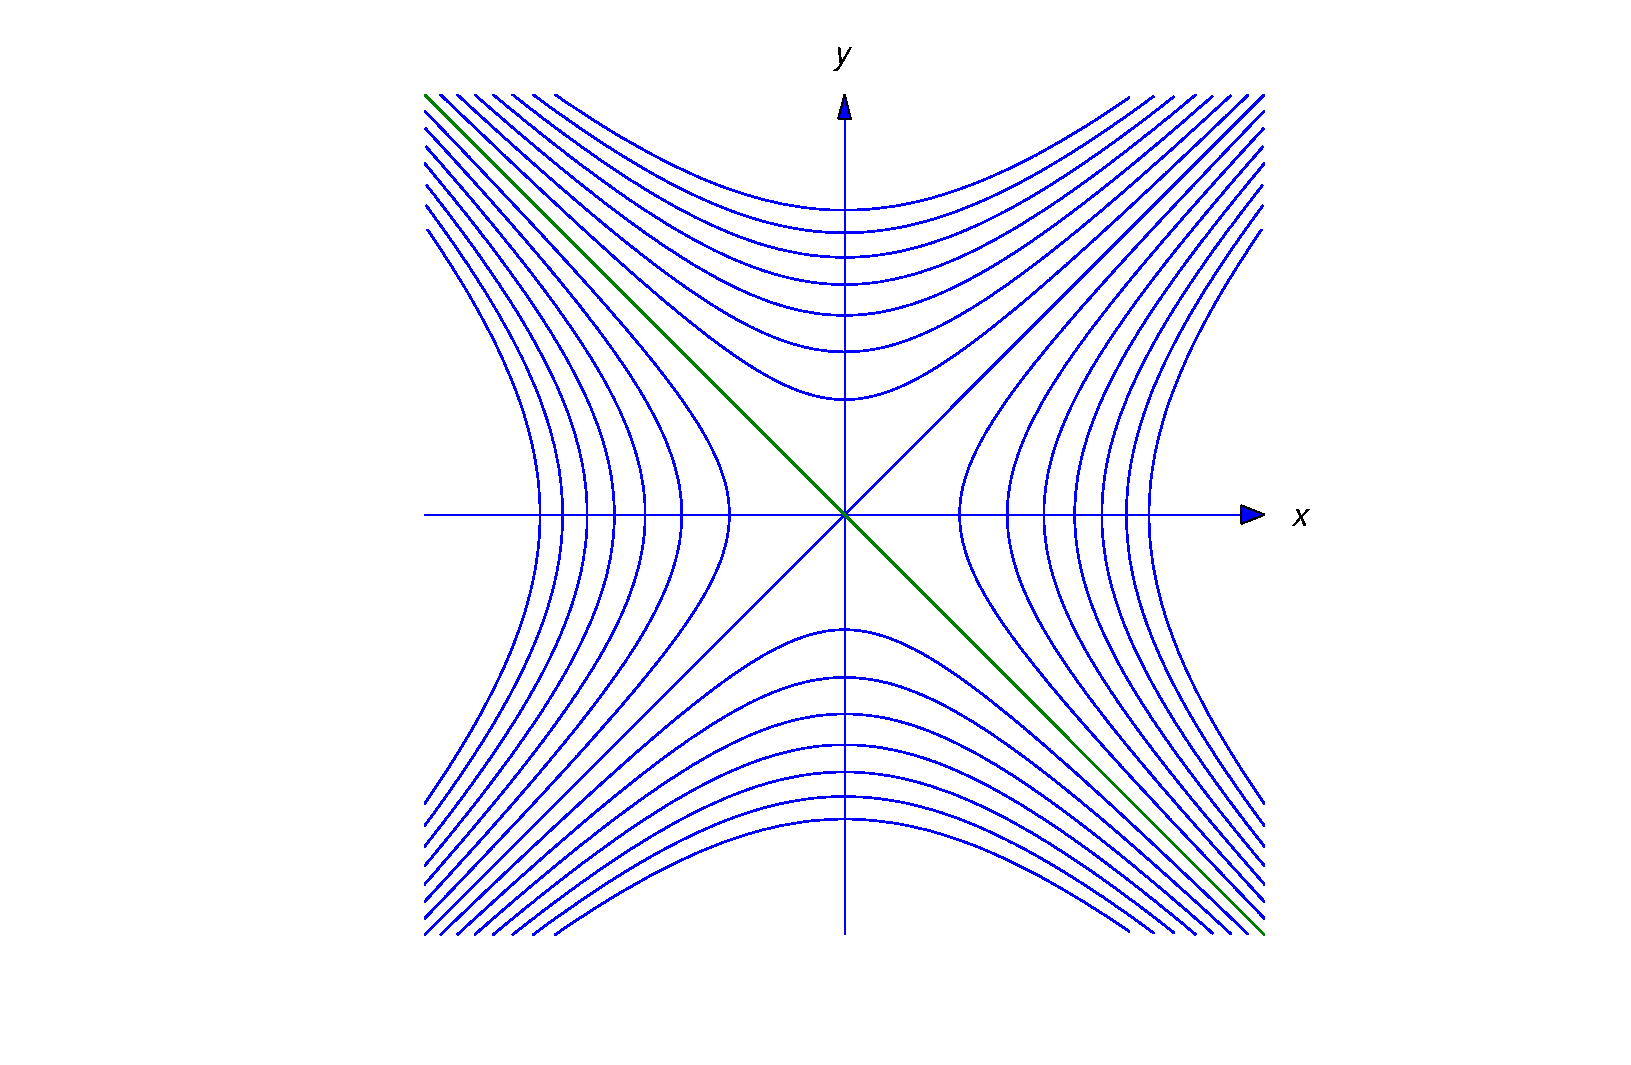
\includegraphics[bb=-78 148 689 643, width=5.67in, height=3.66in, keepaspectratio]{fig040512}
  \relax
  \caption{Orthogonal trajectories of the hyperbolas $xy=c$}
  \label{figure:4.5.12}
\end{figure}
\end{examplesolution}

\setcounter{example}{10}
\setcounter{equation}{18}
\begin{example}
  \rm Find the orthogonal trajectories of the family of circles defined by
  \begin{equation}
    \label{eq:4.5.19}(x-c)^{2}+y^{2}=c^{2}\quad(c\ne0).
  \end{equation}
  These circles are centered on the $x$-axis and tangent to the $y$-axis
  (Figure~\ref{figure:4.5.13}\part{a}).
\end{example}
\setcounter{equation}{19}
\setcounter{figure}{12}
\begin{examplesolution}
\solution Multiplying out the left side of \eqref{eq:4.5.19} yields
\begin{equation}
  \label{eq:4.5.20}x^{2}-2cx+y^{2}=0,
\end{equation}
and differentiating this implicitly with respect to $x$ yields
\begin{equation}
  \label{eq:4.5.21}2(x-c)+2yy'=0.
\end{equation}
From \eqref{eq:4.5.20},
\[
  c=\frac{x^{2}+y^{2}}{2x},
\]
so
\[
  x-c=x-\frac{x^{2}+y^{2}}{2x}=\frac{x^{2}-y^{2}}{2x}.
\]
Substituting this into \eqref{eq:4.5.21} and solving for $y'$ yields
\begin{equation}
  \label{eq:4.5.22}y'=\frac{y^{2}-x^{2}}{2xy}.
\end{equation}
The curves defined by \eqref{eq:4.5.19} are integral curves of \eqref{eq:4.5.22}, and the integral
curves of
\[
  y'=\frac{2xy}{x^{2}-y^{2}}
\]
are orthogonal trajectories of the family \eqref{eq:4.5.19}. This is a homogeneous nonlinear
equation, which we studied in Section~2.4. Substituting $y=ux$ yields
\[
  u'x+u=\frac{2x(ux)}{x^{2}-(ux)^{2}}=\frac{2u}{1-u^{2}},
\]
so
\[
  u'x=\frac{2u}{1-u^{2}}-u=\frac{u(u^{2}+1)}{1-u^{2}},
\]
Separating variables yields
\[
  \frac{1-u^{2}}{u(u^{2}+1)}u'=\frac{1}{x},
\]
or, equivalently,
\[
  \left[\frac{1}{u}-\frac{2u}{u^{2}+1}\right]u'=\frac{1}{x}.
\]
Therefore
\[
  \ln|u|-\ln(u^{2}+1)=\ln|x|+k.
\]
By substituting $u=y/x$, we see that
\[
  \ln|y|-\ln|x|-\ln(x^{2}+y^{2})+\ln(x^{2})=\ln|x|+k,
\]
which, since $\ln(x^{2})=2\ln|x|$, is equivalent to
\[
  \ln|y|-\ln(x^{2}+y^{2})=k,
\]
or
\[
  |y|=e^{k}(x^{2}+y^{2}).
\]
To see what these curves are we rewrite this equation as
\[
  x^{2}+|y|^{2}-e^{-k}|y|=0
\]
and complete the square to obtain
\[
  x^{2}+(|y|-e^{-k}/2)^{2}=(e^{-k}/2)^{2}.
\]
This can be rewritten as
\[
  x^{2}+(y-h)^{2}=h^{2},
\]
where
\[
  h=\left\{
  \begin{array}{rl}
    \dst\frac{e^{-k}}{2}  & \mbox{ if }y\ge 0, \\[\jot]
    -\dst\frac{e^{-k}}{2} & \mbox{ if }y\le0.
  \end{array}\right.
\]
Thus, the orthogonal trajectories are circles centered on the $y$ axis and tangent to the $x$ axis
(Figure~\ref{figure:4.5.13}(b)). The circles for which $h>0$ are above the $x$-axis, while those for
which $h<0$ are below.

\enlargethispage{2in}

\begin{figure}[H]
  \centering
  \scalebox{.9}{
  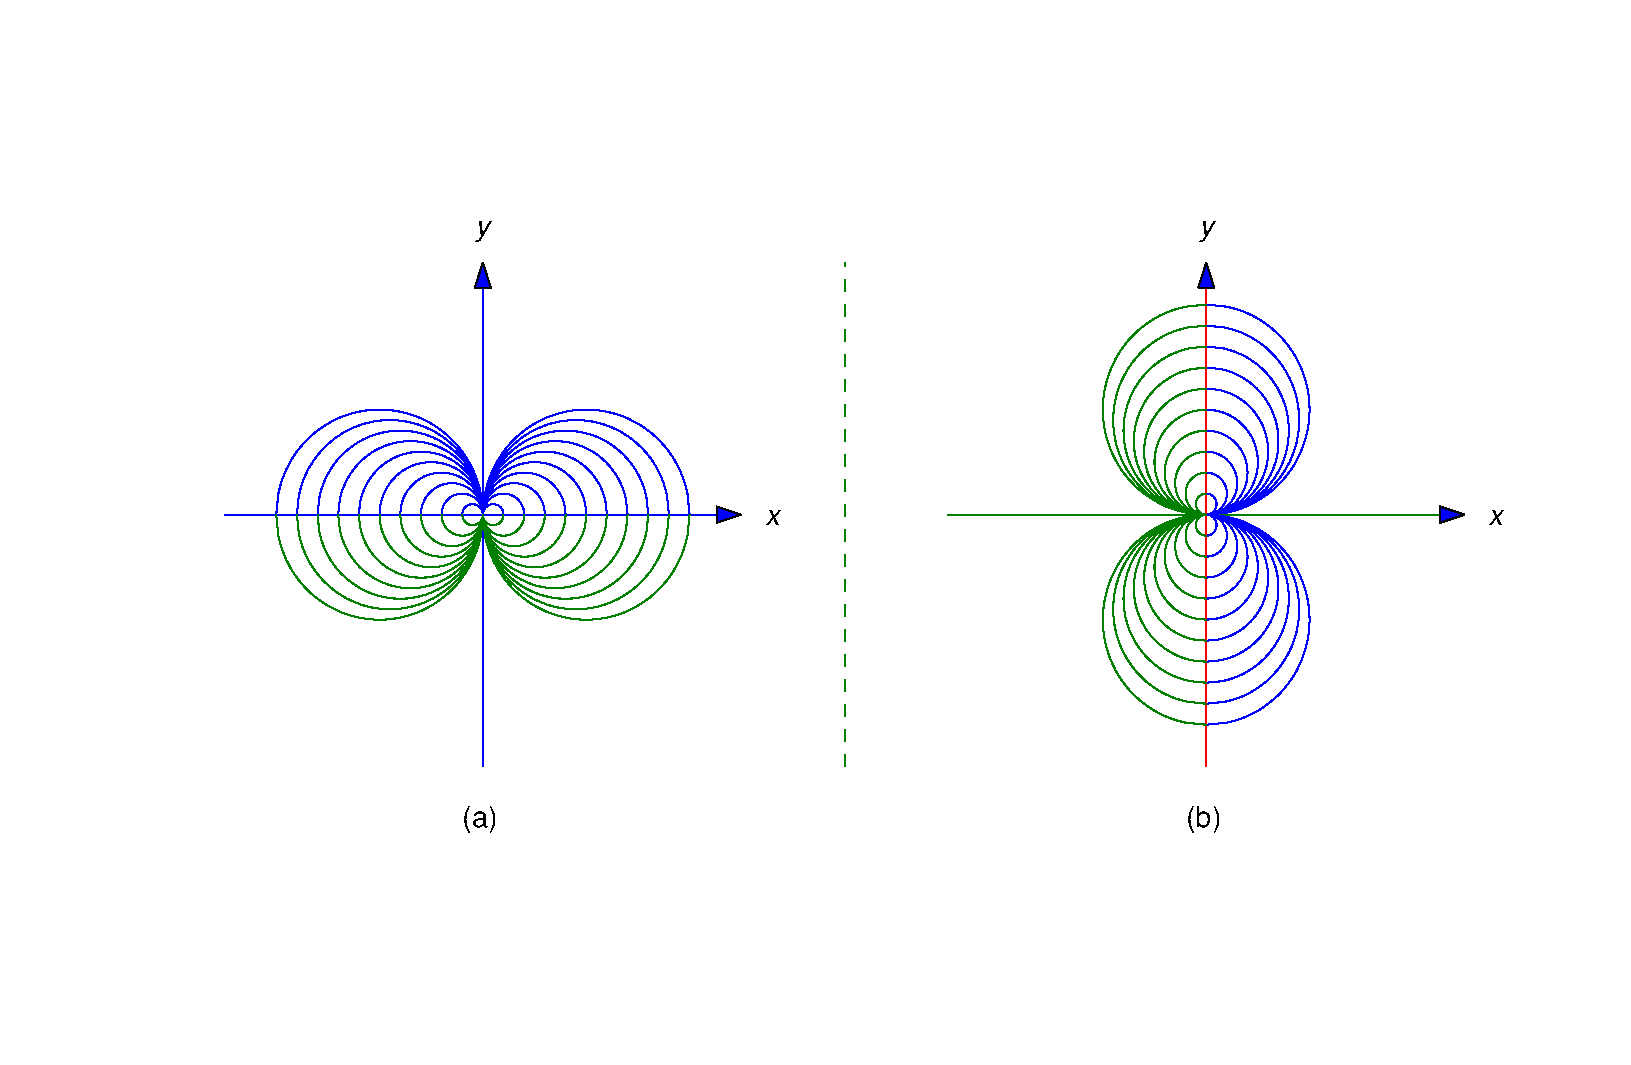
\includegraphics[bb=-78 148 689 643, width=5.67in, height=3.66in, keepaspectratio]{fig040513}}
  \relax
  \caption{{\bf (a)} The circles $(x-c)^{2}+y^{2}=c^{2}$ \, {\bf (b)} The circles $x^{2}+(y-h)^{2}=h^{2}$}
  \vspace*{-40pt}
  \label{figure:4.5.13}
\end{figure}
\end{examplesolution}

\section*{Section 5.1}
\phantomsection
\addcontentsline{toc}{chapter}{Chapter 5}
\setcounter{chapter}{5}
\setcounter{section}{1}

\setcounter{example}{0}
\setcounter{equation}{3}
\begin{example}
  \label{example:5.1.1} \rm The coefficients of $y'$ and $y$ in
  \begin{equation}
    \label{eq:5.1.4}y''-y=0
  \end{equation}
  are the constant functions $p\equiv0$ and $q\equiv-1$, which are continuous on $(-\infty,\infty)$.
  Therefore Theorem~5.1.1 implies that every initial value problem for
  \eqref{eq:5.1.4} has a unique solution on $(-\infty,\infty)$.
  \begin{alist}
    \item % (a)
    Verify that $y_{1}=e^{x}$ and $y_{2}=e^{-x}$ are solutions of \eqref{eq:5.1.4} on
    $(-\infty,\infty)$.

    \item % (b)
    Verify that if $c_{1}$ and $c_{2}$ are arbitrary constants, $y=c_{1}e^{x}+c_{2}e^{-x}$ is a
    solution of \eqref{eq:5.1.4} on $(-\infty,\infty)$.

    \item % (c)
    Solve the initial value problem
    \begin{equation}
      \label{eq:5.1.5}y''-y=0,\quad y(0)=1,\quad y'(0)=3.
    \end{equation}
  \end{alist}
\end{example}
\setcounter{equation}{5}
\begin{examplesolution}
\solutionpart{a} If $y_{1}=e^{x}$ then $y_{1}'=e^{x}$ and $y_{1}''=e^{x}=y_{1}$, so
$y_{1}''-y_{1}=0$. If $y_{2}=e^{-x}$, then $y_{2}'=-e^{-x}$ and $y_{2}''=e^{-x}=y_{2}$, so
$y_{2}''-y_{2}=0$.

\solutionpart{b} If
\begin{equation}
  \label{eq:5.1.6}y=c_{1}e^{x}+c_{2}e^{-x}
\end{equation}
then
\begin{equation}
  \label{eq:5.1.7}y'=c_{1}e^{x}-c_{2}e^{-x}
\end{equation}
and
\[
  y''=c_{1}e^{x}+c_{2}e^{-x},
\]
so
\begin{eqnarray*}
  y''-y & = & (c_{1}e^{x}+c_{2}e^{-x})-(c_{1}e^{x}+c_{2}e^{-x}) \\
        & = & c_{1}(e^{x}-e^{x})+c_{2}(e^{-x}-e^{-x})=0
\end{eqnarray*}
for all $x$. Therefore $y=c_{1}e^{x}+c_{2}e^{-x}$ is a solution of \eqref{eq:5.1.4} on
$(-\infty,\infty)$.

\solutionpart{c} We can solve \eqref{eq:5.1.5} by choosing $c_{1}$ and $c_{2}$ in \eqref{eq:5.1.6}
so that $y(0)=1$ and $y'(0)=3$. Setting $x=0$ in \eqref{eq:5.1.6} and \eqref{eq:5.1.7} shows that
this is equivalent to
\begin{eqnarray*}
  c_{1}+c_{2} & = & 1 \\
  c_{1}-c_{2} & = & 3.
\end{eqnarray*}
Solving these equations yields $c_{1}=2$ and $c_{2}=-1$. Therefore $y=2e^{x}-e^{-x}$ is the unique
solution of \eqref{eq:5.1.5} on $(-\infty,\infty)$.
\end{examplesolution}

\setcounter{example}{1}
\setcounter{equation}{7}
\begin{example}
  \label{example:5.1.2} \rm %\newcommand{\exampletrig}
  Let $\omega$ be a positive constant. The coefficients of $y'$ and $y$ in
  \begin{equation}
    \label{eq:5.1.8}y''+\omega^{2}y=0
  \end{equation}
  are the constant functions $p\equiv0$ and $q\equiv\omega^{2}$, which are continuous on
  $(-\infty,\infty)$. Therefore Theorem~5.1.1 implies that every initial value problem
  for \eqref{eq:5.1.8} has a unique solution on $(-\infty,\infty)$.
  \begin{alist}
    \item % (a)
    Verify that $y_{1}=\cos\omega x$ and $y_{2}=\sin\omega x$ are solutions of \eqref{eq:5.1.8} on
    $(-\infty,\infty)$.

    \item % (b)
    Verify that if $c_{1}$ and $c_{2}$ are arbitrary constants then
    $y=c_{1}\cos\omega x+c_{2}\sin\omega x$ is a solution of \eqref{eq:5.1.8} on $(-\infty,\infty)$.

    \item % (c)
    Solve the initial value problem
    \begin{equation}
      \label{eq:5.1.9}y''+\omega^{2}y=0,\quad y(0)=1,\quad y'(0)=3.
    \end{equation}
  \end{alist}
\end{example}
\setcounter{equation}{9}
\begin{examplesolution}
\solutionpart{a} If $y_{1}=\cos\omega x$ then $y_{1}'=-\omega\sin\omega x$ and
$y_{1}''=-\omega^{2}\cos\omega x=-\omega^{2}y_{1}$, so $y_{1}''+\omega^{2}y_{1}=0$. If
$y_{2}=\sin\omega x$ then, $y_{2}'=\omega\cos\omega x$ and
$y_{2}''=-\omega^{2}\sin\omega x=-\omega^{2}y_{2}$, so $y_{2}''+\omega^{2}y_{2}=0$.

\solutionpart{b} If
\begin{equation}
  \label{eq:5.1.10}y=c_{1}\cos\omega x+c_{2}\sin\omega x
\end{equation}
then
\begin{equation}
  \label{eq:5.1.11}y'=\omega(-c_{1}\sin\omega x+c_{2}\cos\omega x)
\end{equation}
and
\[
  y''=-\omega^{2}(c_{1}\cos\omega x+c_{2}\sin\omega x),
\]
so
\begin{eqnarray*}
  y''+\omega^{2}y & = & -\omega^{2}(c_{1}\cos\omega x+c_{2}\sin\omega x)+\omega^{2}(c_{1}\cos\omega x+c_{2}\sin\omega x) \\
                  & = & c_{1}\omega^{2}(-\cos\omega x+\cos\omega x)+c_{2}\omega^{2}(-\sin\omega x+\sin\omega x)=0
\end{eqnarray*}
for all $x$. Therefore $y=c_{1}\cos\omega x+c_{2}\sin\omega x$ is a solution of \eqref{eq:5.1.8} on
$(-\infty,\infty)$.

\solutionpart{c} To solve \eqref{eq:5.1.9}, we must choose $c_{1}$ and $c_{2}$ in
\eqref{eq:5.1.10} so that $y(0)=1$ and $y'(0)=3$. Setting $x=0$ in \eqref{eq:5.1.10} and
\eqref{eq:5.1.11} shows that $c_{1}=1$ and $c_{2}=3/\omega$. Therefore
\[
  y=\cos\omega x+\frac{3}{\omega}\sin\omega x
\]
is the unique solution of \eqref{eq:5.1.9} on $(-\infty,\infty)$. \bbox
\end{examplesolution}

\setcounter{example}{2}
\setcounter{equation}{12}
\begin{example}
  \label{example:5.1.3} \rm The equation
  \begin{equation}
    \label{eq:5.1.13}x^{2}y''+xy'-4y=0
  \end{equation}
  has the form of the differential equation in \textup{(5.1.12)}, with $P_{0}(x)=x^{2}$,
  $P_{1}(x)=x$, and $P_{2}(x)=-4$, which are all continuous on $(-\infty,\infty)$. However, since
  $P_{0}(0)=0$ we must consider solutions of \eqref{eq:5.1.13} on $(-\infty,0)$ and $(0,\infty)$. Since
  $P_{0}$ has no zeros on these intervals, Theorem~5.1.1 implies that the initial
  value problem
  \[
    x^{2}y''+xy'-4y=0,\quad y(x_{0})=k_{0},\quad y'(x_{0})=k_{1}
  \]
  has a unique solution on $(0,\infty)$ if $x_{0}>0$, or on $(-\infty,0)$ if $x_{0}<0$.
  \begin{alist}
    \item % (a)
    Verify that $y_{1}=x^{2}$ is a solution of \eqref{eq:5.1.13} on $(-\infty,\infty)$ and
    $y_{2}=1/x^{2}$ is a solution of \eqref{eq:5.1.13} on $(-\infty,0)$ and $(0,\infty)$.

    \item % (b)
    Verify that if $c_{1}$ and $c_{2}$ are any constants then $y=c_{1}x^{2}+c_{2}/x^{2}$ is a
    solution of \eqref{eq:5.1.13} on $(-\infty,0)$ and $(0,\infty)$.

    \item % (c)
    Solve the initial value problem
    \begin{equation}
      \label{eq:5.1.14}x^{2}y''+xy'-4y=0,\quad y(1)=2,\quad y'(1)=0.
    \end{equation}

    \item % (d)
    Solve the initial value problem
    \begin{equation}
      \label{eq:5.1.15}x^{2}y''+xy'-4y=0,\quad y(-1)=2,\quad y'(-1)=0.
    \end{equation}
  \end{alist}
\end{example}
\setcounter{equation}{15}
\begin{examplesolution}
\solutionpart{a} If $y_{1}=x^{2}$ then $y_{1}'=2x$ and $y_{1}''=2$, so
\[
  x^{2}y_{1}''+xy_{1}'-4y_{1}=x^{2}(2)+x(2x)-4x^{2}=0
\]
for $x$ in $(-\infty,\infty)$. If $y_{2}=1/x^{2}$, then $y_{2}'=-2/x^{3}$ and $y_{2}''=6/x^{4}$, so
\[
  x^{2}y_{2}''+xy_{2}'-4y_{2}=x^{2}\left(\frac{6}{x^{4}}\right)-x\left(\frac{2}{x^{3}}\right)-\frac{4}{x^{2}}=0
\]
for $x$ in $(-\infty,0)$ or $(0,\infty)$.

\solutionpart{b} If
\begin{equation}
  \label{eq:5.1.16}y=c_{1}x^{2}+\frac{c_{2}}{x^{2}}
\end{equation}
then
\begin{equation}
  \label{eq:5.1.17}y'=2c_{1}x-\frac{2c_{2}}{x^{3}}
\end{equation}
and
\[
  y''=2c_{1}+\frac{6c_{2}}{x^{4}},
\]
so
\begin{eqnarray*}
  x^{2}y''+xy'-4y & = & x^{2}\dst{\left(2c_{1}+\frac{6c_{2}}{x^{4}}\right)}+x\dst{\left(2c_{1}x-\frac{2c_{2}}{x^{3}}\right)}-4\dst{\left(c_{1}x^{2}+\frac{c_{2}}{x^{2}}\right)} \\[2\jot]
                  & = & c_{1}(2x^{2}+2x^{2}-4x^{2})+c_{2}\dst{\left(\frac{6}{x^{2}}-\frac{2}{x^{2}}-\frac{4}{x^{2}}\right)}                                                     \\[2\jot]
                  & = & c_{1}\cdot0+c_{2}\cdot0=0
\end{eqnarray*}
for $x$ in $(-\infty,0)$ or $(0,\infty)$.

\solutionpart{c} To solve \eqref{eq:5.1.14}, we choose $c_{1}$ and $c_{2}$ in \eqref{eq:5.1.16} so
that $y(1)=2$ and $y'(1)=0$. Setting $x=1$ in \eqref{eq:5.1.16} and \eqref{eq:5.1.17} shows that
this is equivalent to
\begin{eqnarray*}
  \phantom{2}c_{1}+\phantom{2}c_{2} & = & 2 \\
  2c_{1}-2c_{2}                     & = & 0.
\end{eqnarray*}
Solving these equations yields $c_{1}=1$ and $c_{2}=1$. Therefore $y=x^{2}+1/x^{2}$ is the unique
solution of \eqref{eq:5.1.14} on $(0,\infty)$.

\solutionpart{d} We can solve \eqref{eq:5.1.15} by choosing $c_{1}$ and $c_{2}$ in \eqref{eq:5.1.16}
so that $y(-1)=2$ and $y'(-1)=0$. Setting $x=-1$ in \eqref{eq:5.1.16} and \eqref{eq:5.1.17} shows
that this is equivalent to
\begin{eqnarray*}
  \phantom{-2}c_{1}+\phantom{2}c_{2} & = & 2 \\
  -2c_{1}+2c_{2}                     & = & 0.
\end{eqnarray*}
Solving these equations yields $c_{1}=1$ and $c_{2}=1$. Therefore $y=x^{2}+1/x^{2}$ is the unique
solution of \eqref{eq:5.1.15} on $(-\infty,0)$. \bbox

Although the {\relax\it formulas\/} for the solutions of \eqref{eq:5.1.14} and
\eqref{eq:5.1.15} are both $y=x^{2}+1/x^{2}$, you should not conclude that these two initial value
problems have the same solution. Remember that a solution of an initial value problem is defined
{\relax\it on an interval that contains the initial point\/}; therefore, the solution of
\eqref{eq:5.1.14} is $y=x^{2}+1/x^{2}$ {\relax\it on the interval\/} $(0,\infty)$, which
contains the initial point $x_{0}=1$, while the solution of \eqref{eq:5.1.15} is $y=x^{2}+1/x^{2}$
{\relax\it on the interval\/} $(-\infty,0)$, which contains the initial point $x_{0}=-1$.
\end{examplesolution}

\setcounter{example}{3}
\begin{example}
  \label{example:5.1.4} \rm \mbox{}
  \newline
  \begin{alist}
    \item % (a)
    Since $e^{x}/e^{-x}=e^{2x}$ is nonconstant, Theorem~5.1.3 implies that
    $y=c_{1}e^{x}+c_{2}e^{-x}$ is the general solution of $y''-y=0$ on $(-\infty,\infty)$.

    \item % (b)
    Since $\cos\omega x/\sin\omega x=\cot\omega x$ is nonconstant, Theorem~5.1.3
    implies that $y=c_{1}\cos\omega x+c_{2}\sin\omega x$ is the general solution of
    $y''+\omega^{2}y=0$ on $(-\infty,\infty)$.

    \item % (c)
    Since $x^{2}/x^{-2}=x^{4}$ is nonconstant, Theorem~5.1.3 implies that
    $y=c_{1}x^{2}+c_{2}/x^{2}$ is the general solution of $x^{2}y''+xy'-4y=0$ on $(-\infty,0)$ and
    $(0,\infty)$.
  \end{alist}
\end{example}

\setcounter{example}{4}
\begin{example}
  \label{example:5.1.5} \rm Verify Abel's formula for the following differential equations and the
  corresponding solutions, from Examples~\ref{example:5.1.1}, \ref{example:5.1.2}, and
  \ref{example:5.1.3}:
  \begin{alist}
    \item % (a)
    $y''-y=0;\quad y_{1}=e^{x},\;y_{2}=e^{-x}$

    \item % (b)
    $y''+\omega^{2}y=0;\quad\quad y_{1}=\cos\omega x,\;y_{2}=\sin\omega x$

    \item % (c)
    $x^{2}y''+xy'-4y=0;\quad y_{1}=x^{2},\;y_{2}=1/x^{2}$
  \end{alist}
\end{example}
\setcounter{equation}{30}
\begin{examplesolution}
\solutionpart{a} Since $p\equiv0$, we can verify Abel's formula by showing that $W$ is constant,
which is true, since
\[
  W(x)=\left|
  \begin{array}{rr}
    e^{x} & e^{-x}  \\[2\jot]
    e^{x} & -e^{-x}
  \end{array}\right|=e^{x}(-e^{-x})-e^{x}e^{-x}=-2
\]
for all $x$.

\solutionpart{b} Again, since $p\equiv0$, we can verify Abel's formula by showing that $W$ is
constant, which is true, since
\begin{eqnarray*}
  W(x)&=&\dst{\left|\begin{array}{cc}\cos\omega x&\sin\omega x\\[2\jot] -\omega\sin\omega x&\omega\cos\omega x\end{array}\right|}\\[2\jot] &=&\cos\omega x(\omega\cos\omega x)-(-\omega\sin\omega x)\sin\omega x\\&=&\omega(\cos^{2}\omega x+\sin^{2}\omega x)=\omega
\end{eqnarray*}
for all $x$.

\solutionpart{c} Computing the Wronskian of $y_{1}=x^{2}$ and $y_{2}=1/x^{2}$ directly yields
\begin{equation}
  \label{eq:5.1.31}W=\left|
  \begin{array}{cc}
    x^{2} & 1/x^{2}  \\[2\jot]
    2x    & -2/x^{3}
  \end{array}\right|=x^{2}\left(-\frac{2}{x^{3}}\right)-2x\left(\frac{1}{x^{2}}\right)=-\frac{4}{x}.
\end{equation}
To verify Abel's formula we rewrite the differential equation as
\[
  y''+\frac{1}{x}y'-\frac{4}{x^{2}}y=0
\]
to see that $p(x)=1/x$. If $x_{0}$ and $x$ are either both in $(-\infty,0)$ or both in $(0,\infty)$
then
\[
  \int_{x_{0}}^{x}p(t)\,dt=\int_{x_{0}}^{x}\frac{dt}{t}=\ln\left(\frac{x}{x_{0}}\right),
\]
so Abel's formula becomes
\begin{eqnarray*}
  W(x) & = & W(x_{0})e^{-\ln(x/x_{0})}=W(x_{0})\frac{x_{0}}{x}                                            \\
       & = & -\left(\frac{4}{x_{0}}\right)\left(\frac{x_{0}}{x}\right)\mbox{\quad from \eqref{eq:5.1.31}} \\
       & = & -\frac{4}{x},
\end{eqnarray*}
which is consistent with \eqref{eq:5.1.31}.\bbox
\end{examplesolution}

\section*{Section 5.2}
\setcounter{chapter}{5}
\setcounter{section}{2}

\setcounter{example}{0}
\setcounter{equation}{3}
\begin{example}
  \label{example:5.2.1}\rm \mbox{}
  \newline
  \begin{alist}
    \item % (a)
    Find the general solution of
    \begin{equation}
      \label{eq:5.2.4}y''+6y'+5y=0.
    \end{equation}

    \item % (b)
    Solve the initial value problem
    \begin{equation}
      \label{eq:5.2.5}y''+6y'+5y=0,\quad y(0)=3,\;y'(0)=-1.
    \end{equation}
  \end{alist}
\end{example}
\setcounter{equation}{5}
\setcounter{figure}{0}
\begin{examplesolution}
\solutionpart{a} The characteristic polynomial of \eqref{eq:5.2.4} is
\[
  p(r)=r^{2}+6r+5=(r+1)(r+5).
\]
Since $p(-1)=p(-5)=0$, $y_{1}=e^{-x}$ and $y_{2}=e^{-5x}$ are solutions of \eqref{eq:5.2.4}. Since
$y_{2}/y_{1}=e^{-4x}$ is nonconstant, 5.1.6 implies that the general solution of
\eqref{eq:5.2.4} is
\begin{equation}
  \label{eq:5.2.6}y=c_{1}e^{-x}+c_{2}e^{-5x}.
\end{equation}

\solutionpart{b} We must determine $c_{1}$ and $c_{2}$ in \eqref{eq:5.2.6} so that $y$ satisfies the
initial conditions in \eqref{eq:5.2.5}. Differentiating \eqref{eq:5.2.6} yields
\begin{equation}
  \label{eq:5.2.7}y'=-c_{1}e^{-x}-5c_{2}e^{-5x}.
\end{equation}
Imposing the initial conditions $y(0)=3$, $y'(0)=-1$ in \eqref{eq:5.2.6} and \eqref{eq:5.2.7} yields
\[
  \begin{array}{rcr}
    \phantom{-}c_{1}+\phantom{5}c_{2} & = & 3\phantom{.} \\
    -c_{1}-5c_{2}                     & = & -1.
  \end{array}
\]
The solution of this system is $c_{1}=7/2$, $c_{2}=-1/2$. Therefore the solution of \eqref{eq:5.2.5}
is
\[
  y=\frac{7}{2}e^{-x}-\frac{1}{2}e^{-5x}.
\]
Figure~\ref{figure:5.2.1} is a graph of this solution.

\begin{figure}[H]
  \centering
  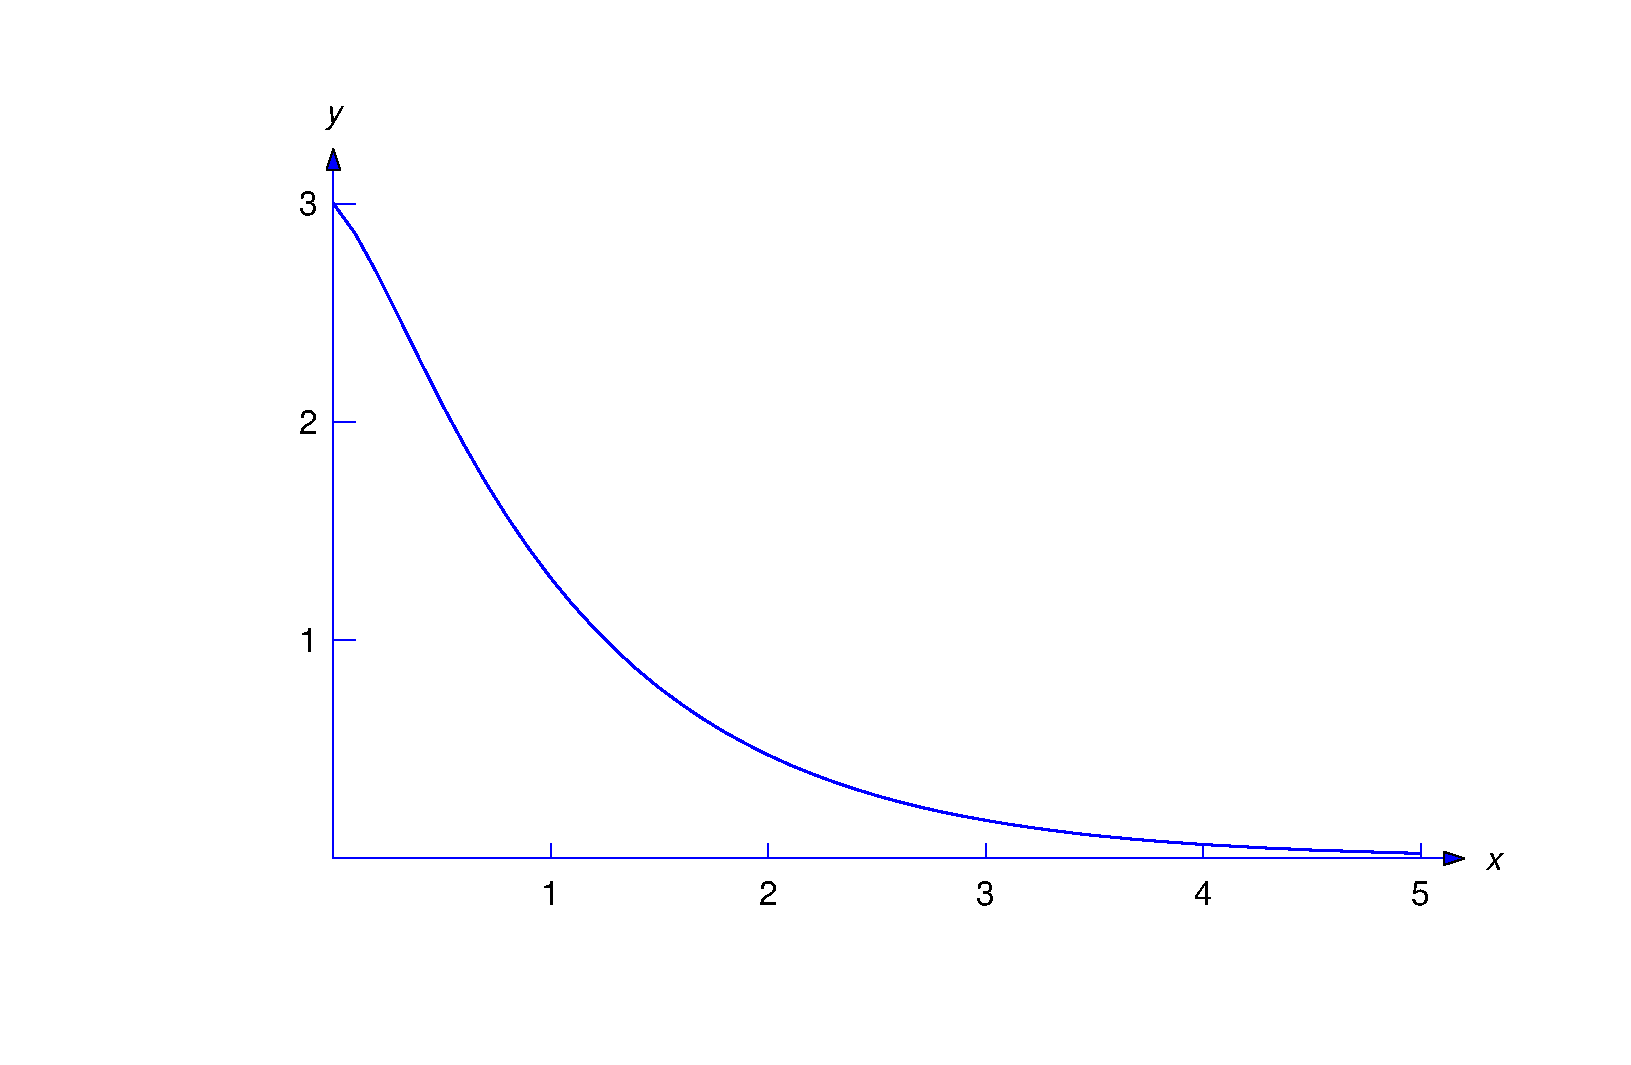
\includegraphics[bb=-78 148 689 643, width=5.67in, height=3.66in, keepaspectratio]{fig050201}
  \relax
  \caption{$y=\dst{\frac{7}{2}e^{-x}-\frac{1}{2}e^{-5x}}$ }
  \label{figure:5.2.1}
\end{figure}
\end{examplesolution}

\setcounter{example}{1}
\setcounter{equation}{7}
\begin{example}
  \label{example:5.2.2}\rm \mbox{}
  \newline
  \begin{alist}
    \item % (a)
    Find the general solution of
    \begin{equation}
      \label{eq:5.2.8}y''+6y'+9y=0.
    \end{equation}

    \item % (b)
    Solve the initial value problem
    \begin{equation}
      \label{eq:5.2.9}y''+6y'+9y=0,\quad y(0)=3,\;y'(0)=-1.
    \end{equation}
  \end{alist}
\end{example}
\setcounter{equation}{9}
\setcounter{figure}{1}
\begin{examplesolution}
\solutionpart{a} The characteristic polynomial of \eqref{eq:5.2.8} is
\[
  p(r)=r^{2}+6r+9=(r+3)^{2},
\]
so the characteristic equation has the repeated real root $r_{1}=-3$. Therefore $y_{1}=e^{-3x}$ is a
solution of \eqref{eq:5.2.8}. Since the characteristic equation has no other roots, \eqref{eq:5.2.8}
has no other solutions of the form $e^{rx}$. We look for solutions of the form $y=uy_{1}=ue^{-3x}$,
where $u$ is a function that we'll now determine. (This should remind you of the method of variation
of parameters used in Section~2.1 to solve the nonhomogeneous equation $y'+p(x)y=f(x)$, given a
solution $y_{1}$ of the complementary equation $y'+p(x)y=0$. It's also a special case of a method
called {\relax\it reduction of order\/} that we'll study in Section~5.6. For other ways to
obtain a second solution of \eqref{eq:5.2.8} that's not a multiple of $e^{-3x}$, see
Exercises~5.1.~\hspace*{-3pt}5.1.9, 5.1.~\hspace*{-3pt}5.1.12, and
5.2.33.

If $y=ue^{-3x}$, then
\[
  y'=u'e^{-3x}-3ue^{-3x}\mbox{\quad and \quad}y''=u''e^{-3x}-6u'e^{-3x}+9ue^{-3x},
\]
so
\begin{eqnarray*}
  y''+6y'+9y & = & e^{-3x}\left[(u''-6u'+9u)+6(u'-3u)+9u\right] \\
             & = & e^{-3x}\left[u''-(6-6)u'+(9-18+9)u\right]=u''e^{-3x}.
\end{eqnarray*}
Therefore $y=ue^{-3x}$ is a solution of \eqref{eq:5.2.8} if and only if $u''=0$, which is equivalent
to $u=c_{1}+c_{2}x$, where $c_{1}$ and $c_{2}$ are constants. Therefore any function of the form
\begin{equation}
  \label{eq:5.2.10}y=e^{-3x}(c_{1}+c_{2}x)
\end{equation}
is a solution of \eqref{eq:5.2.8}. Letting $c_{1}=1$ and $c_{2}=0$ yields the solution
$y_{1}=e^{-3x}$ that we already knew. Letting $c_{1}=0$ and $c_{2}=1$ yields the second solution
$y_{2}=xe^{-3x}$. Since $y_{2}/y_{1}=x$ is nonconstant, 5.1.6 implies that
$\{y_{1},y_{2}\}$ is fundamental set of solutions of \eqref{eq:5.2.8}, and \eqref{eq:5.2.10} is the
general solution.

\solutionpart{b} Differentiating \eqref{eq:5.2.10} yields
\begin{equation}
  \label{eq:5.2.11}y'=-3e^{-3x}(c_{1}+c_{2}x)+c_{2}e^{-3x}.
\end{equation}
Imposing the initial conditions $y(0)=3$, $y'(0)=-1$ in \eqref{eq:5.2.10} and \eqref{eq:5.2.11}
yields $c_{1}=3$ and $-3c_{1}+c_{2}=-1$, so $c_{2}=8$. Therefore the solution of \eqref{eq:5.2.9} is
\[
  y=e^{-3x}(3+8x).
\]
Figure~\ref{figure:5.2.2} is a graph of this solution.

\enlargethispage{2in}

\begin{figure}[H]
  \centering
  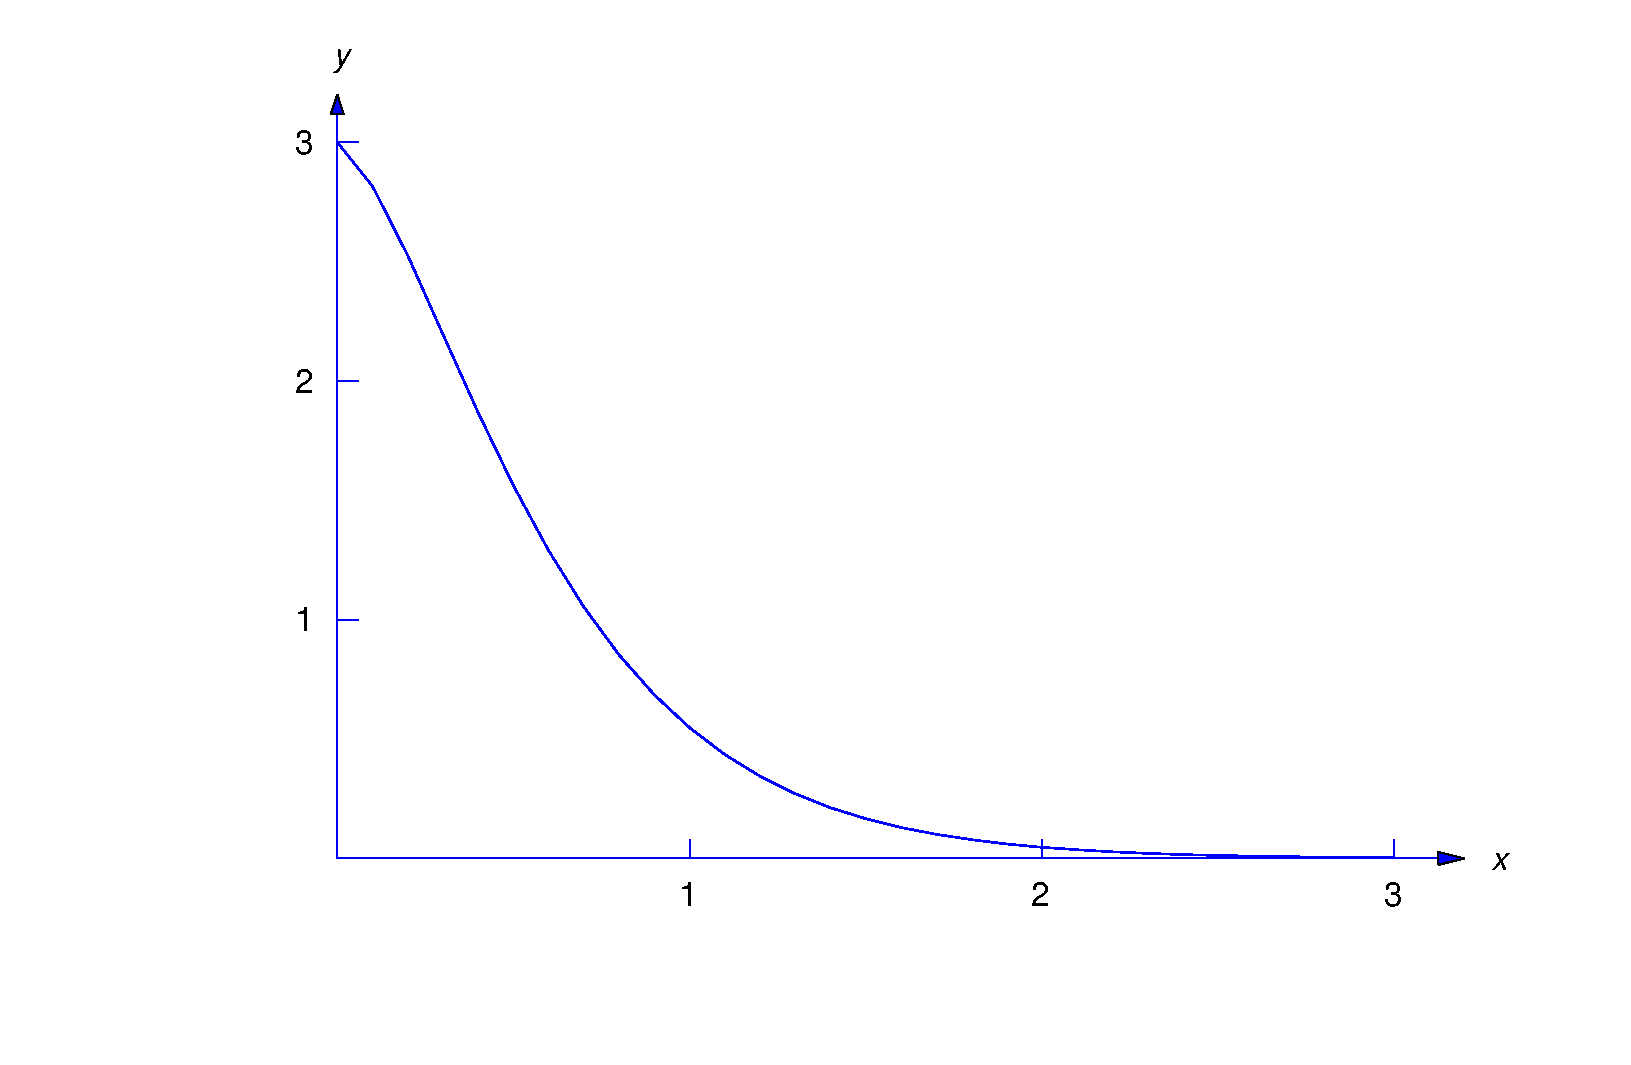
\includegraphics[bb=-78 148 689 643, width=5.67in, height=3.66in, keepaspectratio]{fig050202}
  \relax
  \vspace*{-10pt}
  \caption{$y=e^{-3x}(3+8x)$}
  \label{figure:5.2.2}
\end{figure}
\end{examplesolution}

\setcounter{example}{2}
\setcounter{equation}{13}
\begin{example}
  \label{example:5.2.3}\rm \mbox{}
  \newline
  \begin{alist}
    \item % (a)
    Find the general solution of
    \begin{equation}
      \label{eq:5.2.14}y''+4y'+13y=0.
    \end{equation}

    \item % (b)
    Solve the initial value problem
    \begin{equation}
      \label{eq:5.2.15}y''+4y'+13y=0,\quad y(0)=2,\;y'(0)=-3.
    \end{equation}
  \end{alist}
\end{example}
\setcounter{equation}{15}
\setcounter{figure}{2}
\begin{examplesolution}
\solutionpart{a} The characteristic polynomial of \eqref{eq:5.2.14} is
\[
  p(r)=r^{2}+4r+13=r^{2}+4r+4+9=(r+2)^{2}+9.
\]
The roots of the characteristic equation are $r_{1}=-2+3i$ and $r_{2}=-2-3i$. By analogy with
Case~1, it's reasonable to expect that $e^{(-2+3i)x}$ and $e^{(-2-3i)x}$ are solutions of
\eqref{eq:5.2.14}. This is true (see Exercise~5.2.34); however, there are difficulties
here, since you are probably not familiar with exponential functions with complex arguments, and
even if you are, it's inconvenient to work with them, since they are complex--valued. We'll take a
simpler approach, which we motivate as follows: the exponential notation suggests that
\[
  e^{(-2+3i)x}=e^{-2x}e^{3ix}\mbox{\quad and \quad}e^{(-2-3i)x}=e^{-2x}e^{-3ix},
\]
so even though we haven't defined $e^{3ix}$ and $e^{-3ix}$, it's reasonable to expect that every
linear combination of $e^{(-2+3i)x}$ and $e^{(-2-3i)x}$ can be written as $y=ue^{-2x}$, where $u$
depends upon $x$. To determine $u$, we note that if $y=ue^{-2x}$ then
\[
  y'=u'e^{-2x}-2ue^{-2x}\mbox{\quad and \quad}y''=u''e^{-2x}-4u'e^{-2x}+4ue^{-2x},
\]
so
\begin{eqnarray*}
  y''+4y'+13y & = & e^{-2x}\left[(u''-4u'+4u)+4(u'-2u)+13u\right] \\
              & = & e^{-2x}\left[u''-(4-4)u'+(4-8+13)u\right]=e^{-2x}(u''+9u).
\end{eqnarray*}
Therefore $y=ue^{-2x}$ is a solution of \eqref{eq:5.2.14} if and only if
\[
  u''+9u=0.
\]
From Example~\ref{example:5.1.2}, the general solution of this equation is
\[
  u=c_{1}\cos3x+c_{2}\sin3x.
\]
Therefore any function of the form
\begin{equation}
  \label{eq:5.2.16}y=e^{-2x}(c_{1}\cos3x+c_{2}\sin3x)
\end{equation}
is a solution of \eqref{eq:5.2.14}. Letting $c_{1}=1$ and $c_{2}=0$ yields the solution
$y_{1}=e^{-2x}\cos3x$. Letting $c_{1}=0$ and $c_{2}=1$ yields the second solution
$y_{2}=e^{-2x}\sin3x$. Since $y_{2}/y_{1}=\tan3x$ is nonconstant, 5.1.6 implies that
$\{y_{1},y_{2}\}$ is a fundamental set of solutions of \eqref{eq:5.2.14}, and \eqref{eq:5.2.16} is
the general solution.

\solutionpart{b} Imposing the condition $y(0)=2$ in \eqref{eq:5.2.16} shows that $c_{1}=2$.
Differentiating \eqref{eq:5.2.16} yields
\[
  y'=-2e^{-2x}(c_{1}\cos3x+c_{2}\sin3x)+3e^{-2x}(-c_{1}\sin3x+c_{2}\cos3x),
\]
and imposing the initial condition $y'(0)=-3$ here yields $-3=-2c_{1}+3c_{2}=-4+3c_{2}$, so
$c_{2}=1/3$. Therefore the solution of \eqref{eq:5.2.15} is
\[
  y=e^{-2x}(2\cos3x+\frac{1}{3}\sin3x).
\]
Figure~\ref{figure:5.2.3} is a graph of this function. \bbox

\begin{figure}[H]
  \centering
  \relax
  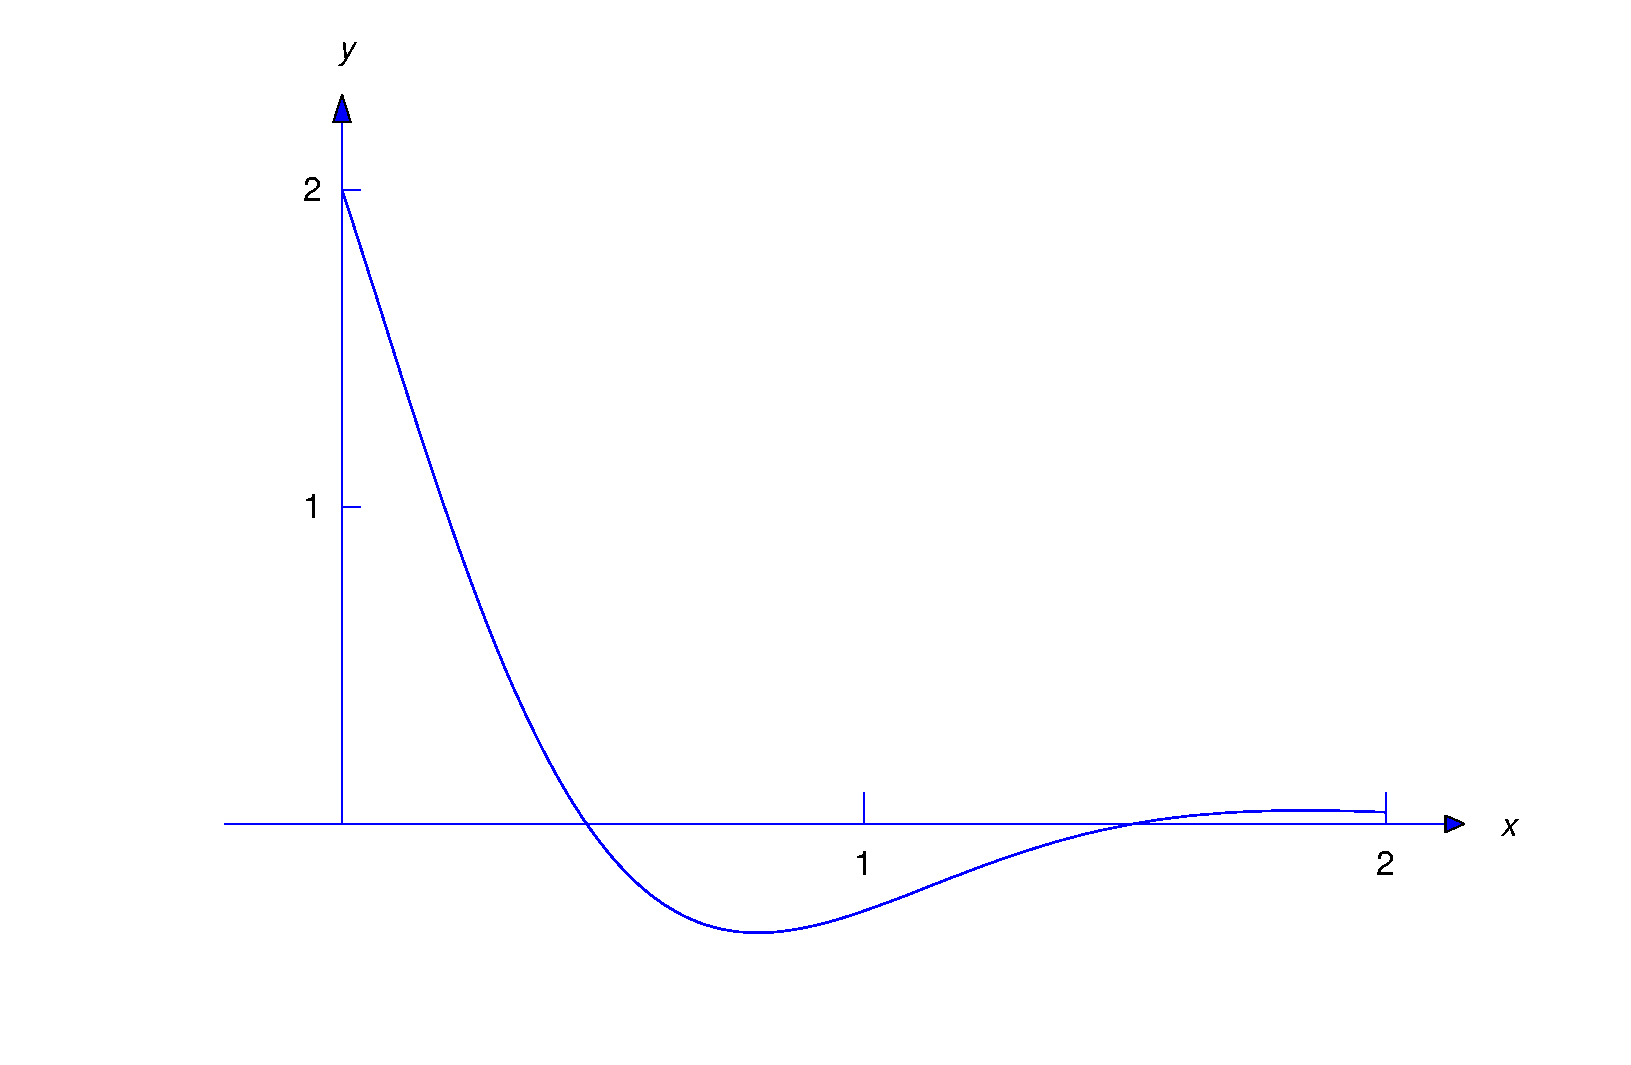
\includegraphics[bb=-78 148 689 643, width=5.67in, height=3.66in, keepaspectratio]{fig050203}
  \caption{$\dst{y=e^{-2x}(2\cos3x+\frac{1}{3}\sin3x)}$}
  \label{figure:5.2.3}
\end{figure}
\end{examplesolution}

\section*{Section 5.3}
\setcounter{chapter}{5}
\setcounter{section}{3}

\setcounter{example}{0}
\setcounter{equation}{6}
\begin{example}
  \label{example:5.3.1} \rm \mbox{}
  \newline
  \begin{alist}
    \item % (a)
    Find the general solution of
    \begin{equation}
      \label{eq:5.3.7}y''+y=1.
    \end{equation}

    \item % (b)
    Solve the initial value problem
    \begin{equation}
      \label{eq:5.3.8}y''+y=1,\quad y(0)=2,\quad y'(0)=7.
    \end{equation}
  \end{alist}
\end{example}
\setcounter{equation}{8}
\setcounter{figure}{0}
\begin{examplesolution}
\solutionpart{a} We can apply Theorem~5.3.2 with $(a,b)=(-\infty,\infty)$, since the
functions $p\equiv0$, $q\equiv1$, and $f\equiv1$ in \eqref{eq:5.3.7} are continuous on
$(-\infty,\infty)$. By inspection we see that $y_{p}\equiv1$ is a particular solution of
\eqref{eq:5.3.7}. Since $y_{1}=\cos x$ and $y_{2}=\sin x$ form a fundamental set of solutions of the
complementary equation $y''+y=0$, the general solution of \eqref{eq:5.3.7} is
\begin{equation}
  \label{eq:5.3.9}y=1+c_{1}\cos x+c_{2}\sin x.
\end{equation}

\solutionpart{b} Imposing the initial condition $y(0)=2$ in \eqref{eq:5.3.9} yields $2=1+c_{1}$, so
$c_{1}=1$. Differentiating \eqref{eq:5.3.9} yields
\[
  y'=-c_{1}\sin x+c_{2}\cos x.
\]
Imposing the initial condition $y'(0)=7$ here yields $c_{2}=7$, so the solution of \eqref{eq:5.3.8}
is
\[
  y=1+\cos x+7\sin x.
\]
Figure~\ref{figure:5.3.1} is a graph of this function.

\begin{figure}[H]
  \centering
  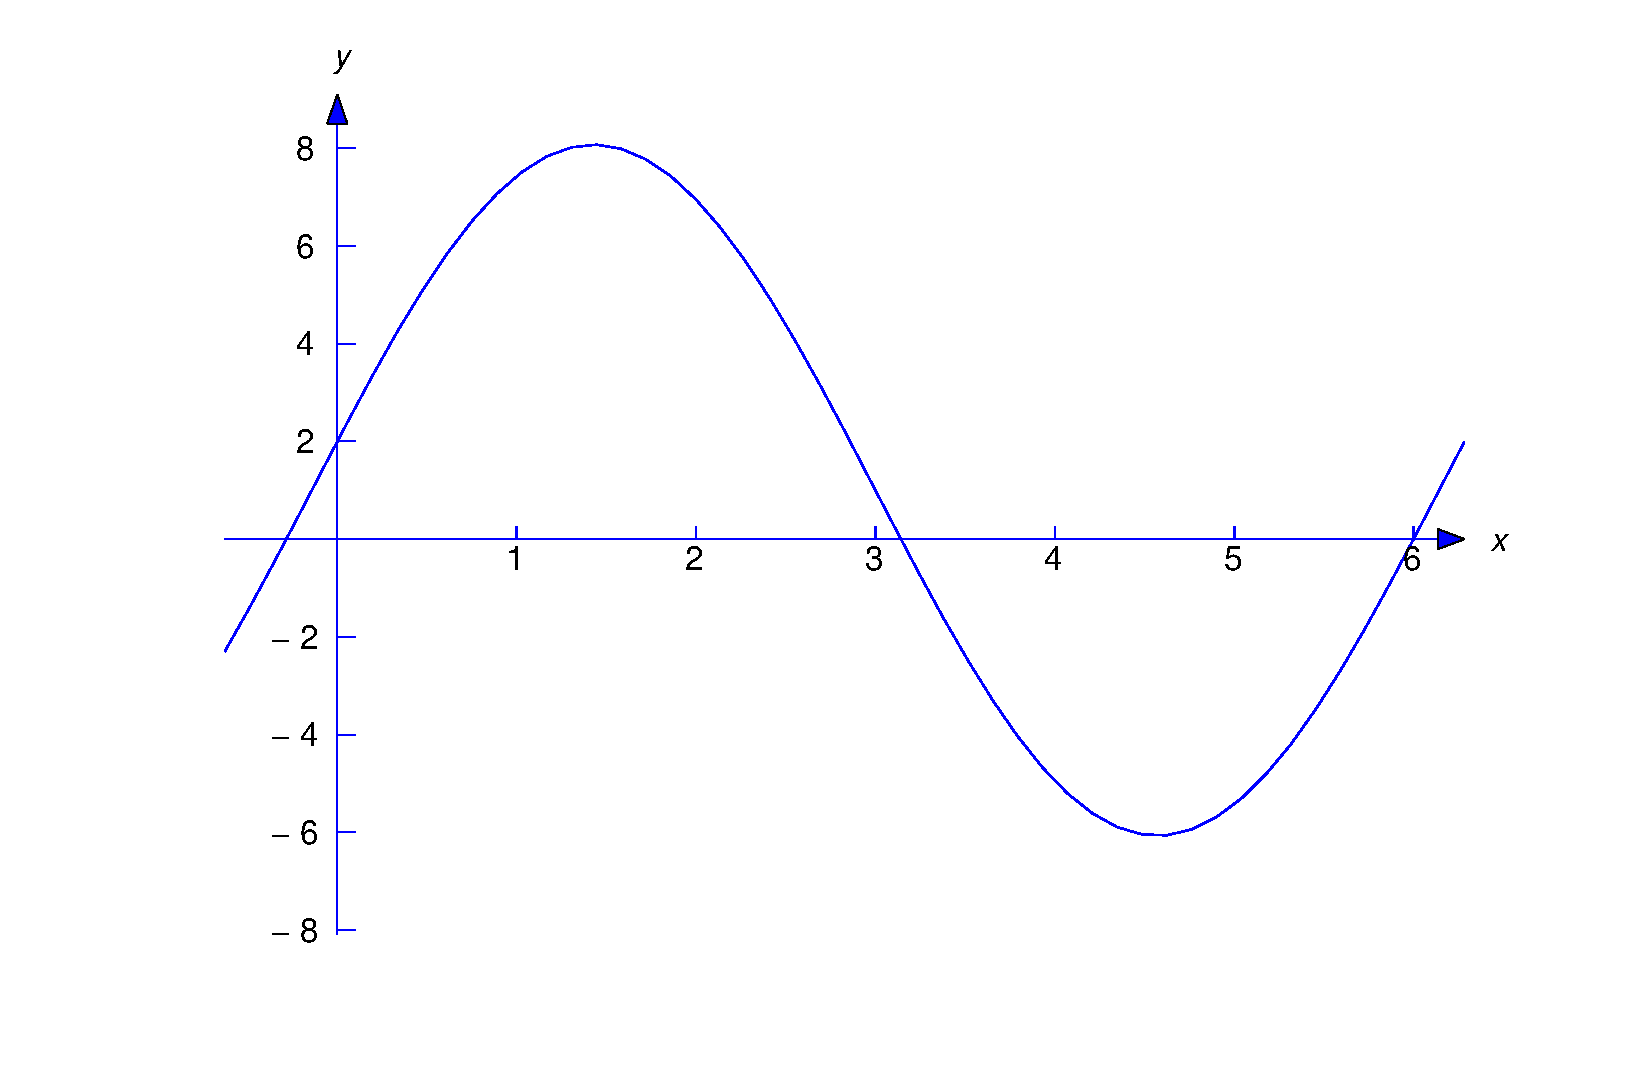
\includegraphics[bb=-78 148 689 643, width=5.67in, height=3.66in, keepaspectratio]{fig050301}
  \relax
  \caption{$y=1+\cos x+7\sin x$}
  \label{figure:5.3.1}
\end{figure}
\end{examplesolution}

\setcounter{example}{1}
\setcounter{equation}{9}
\begin{example}
  \label{example:5.3.2} \rm \mbox{}
  \newline %\examplepoly
  \begin{alist}
    \item % (a)
    Find the general solution of
    \begin{equation}
      \label{eq:5.3.10}y''-2y'+y=-3-x+x^{2}.
    \end{equation}

    \item % (b)
    Solve the initial value problem
    \begin{equation}
      \label{eq:5.3.11}y''-2y'+y=-3-x+x^{2},\quad y(0)=-2,\quad y'(0)=1.
    \end{equation}
  \end{alist}
\end{example}
\setcounter{equation}{11}
\setcounter{figure}{1}
\begin{examplesolution}
\solutionpart{a} The characteristic polynomial of the complementary equation
\[
  y''-2y'+y=0
\]
is $r^{2}-2r+1=(r-1)^{2}$, so $y_{1}=e^{x}$ and $y_{2}=xe^{x}$ form a fundamental set of solutions
of the complementary equation. To guess a form for a particular solution of \eqref{eq:5.3.10}, we
note that substituting a second degree polynomial $y_{p}=A+Bx+Cx^{2}$ into the left side of
\eqref{eq:5.3.10} will produce another second degree polynomial with coefficients that depend upon
$A$, $B$, and $C$. The trick is to choose $A$, $B$, and $C$ so the polynomials on the two sides of
\eqref{eq:5.3.10} have the same coefficients; thus, if
\[
  y_{p}=A+Bx+Cx^{2}\mbox{\quad then \quad}y_{p}'=B+2Cx\mbox{\quad and \quad}y_{p}''=2C,
\]
so
\begin{eqnarray*}
  y_{p}''-2y_{p}'+y_{p} & = & 2C-2(B+2Cx)+(A+Bx+Cx^{2}) \\
                        & = & (2C-2B+A)+(-4C+B)x+Cx^{2}=-3-x+x^{2}.
\end{eqnarray*}
Equating coefficients of like powers of $x$ on the two sides of the last equality yields
\begin{eqnarray*}
  C       & = & \phantom{-}1\phantom{.} \\
  B-4C    & = & -1\phantom{.}           \\
  A-2B+2C & = & -3,
\end{eqnarray*}
so $C=1$, $B=-1+4C=3$, and $A=-3-2C+2B=1$. Therefore $y_{p}=1+3x+x^{2}$ is a particular solution of
\eqref{eq:5.3.10} and Theorem~5.3.2 implies that
\begin{equation}
  \label{eq:5.3.12}y=1+3x+x^{2}+e^{x}(c_{1}+c_{2}x)
\end{equation}
is the general solution of \eqref{eq:5.3.10}.

\solutionpart{b} Imposing the initial condition $y(0)=-2$ in \eqref{eq:5.3.12} yields $-2=1+c_{1}$,
so $c_{1}=-3$. Differentiating \eqref{eq:5.3.12} yields
\[
  y'=3+2x+e^{x}(c_{1}+c_{2}x)+c_{2}e^{x},
\]
and imposing the initial condition $y'(0)=1$ here yields $1=3+c_{1}+c_{2}$, so $c_{2}=1$. Therefore
the solution of \eqref{eq:5.3.11} is
\[
  y=1+3x+x^{2}-e^{x}(3-x).
\]
Figure~\ref{figure:5.3.2} is a graph of this solution.

\begin{figure}[H]
  \centering
  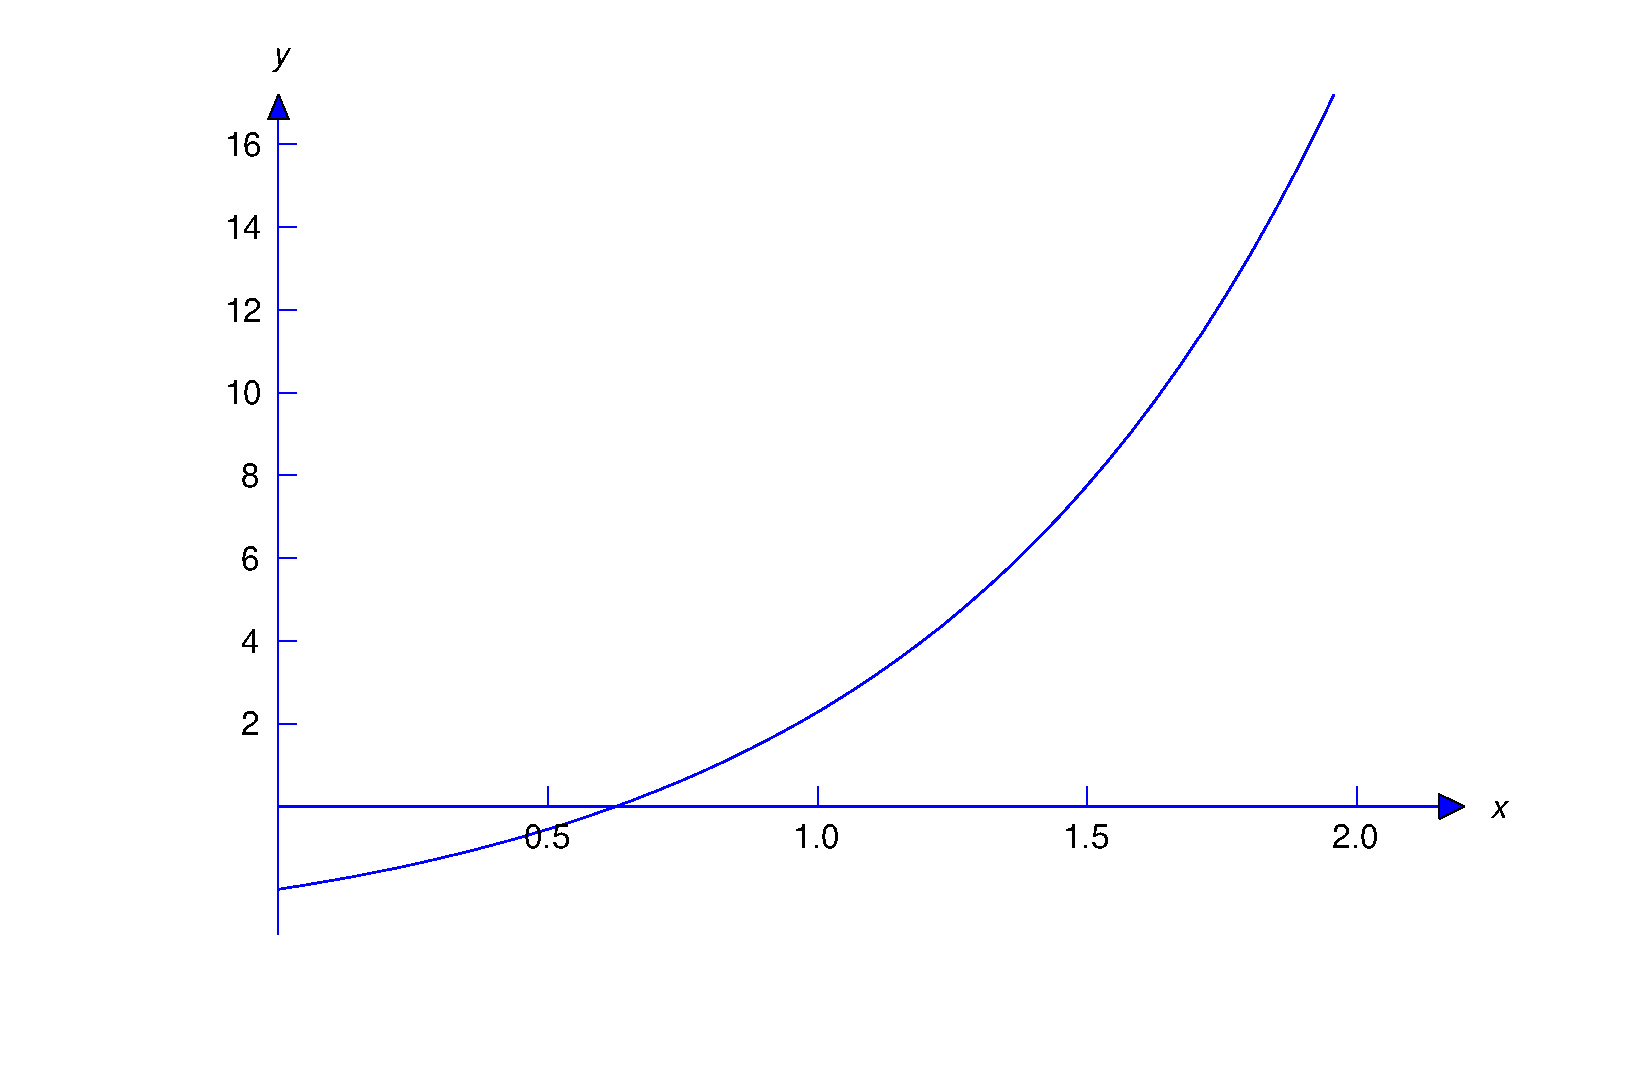
\includegraphics[bb=-78 148 689 643, width=5.67in, height=3.66in, keepaspectratio]{fig050302}
  \relax
  \caption{$y=1+3x+x^{2}-e^{x}(3-x)$}
  \label{figure:5.3.2}
\end{figure}
\end{examplesolution}

\setcounter{example}{2}
\setcounter{equation}{12}
\begin{example}
  \label{example:5.3.3} \rm Find the general solution of
  \begin{equation}
    \label{eq:5.3.13}x^{2}y''+xy'-4y=2x^{4}
  \end{equation}
  on $(-\infty,0)$ and $(0,\infty)$.
\end{example}
\begin{examplesolution}
\solution In Example~\ref{example:5.1.3}, we verified that $y_{1}=x^{2}$ and $y_{2}=1/x^{2}$ form a
fundamental set of solutions of the complementary equation
\[
  x^{2}y''+xy'-4y=0
\]
on $(-\infty,0)$ and $(0,\infty)$. To find a particular solution of \eqref{eq:5.3.13}, we note that
if $y_{p}=Ax^{4}$, where $A$ is a constant then both sides of \eqref{eq:5.3.13} will be constant
multiples of $x^{4}$ and we may be able to choose $A$ so the two sides are equal. This is true in
this example, since if $y_{p}=Ax^{4}$ then
\[
  x^{2}y_{p}''+xy_{p}'-4y_{p}=x^{2}(12Ax^{2})+x(4Ax^{3})-4Ax^{4}=12Ax^{4}=2x^{4}
\]
if $A=1/6$; therefore, $y_{p}=x^{4}/6$ is a particular solution of \eqref{eq:5.3.13} on
$(-\infty,\infty)$. Theorem~5.3.2 implies that the general solution of
\eqref{eq:5.3.13} on $(-\infty,0)$ and $(0,\infty)$ is
\[
  y=\frac{x^{4}}{6}+c_{1}x^{2}+\frac{c_{2}}{x^{2}}.
\]
\end{examplesolution}

\setcounter{example}{3}
\setcounter{equation}{14}
\begin{example}
  \label{example:5.3.4} \rm The function $y_{p_{1}}=x^{4}/15$ is a particular solution of
  \begin{equation}
    \label{eq:5.3.15}x^{2}y''+4xy'+2y=2x^{4}
  \end{equation}
  on $(-\infty,\infty)$ and $y_{p_{2}}=x^{2}/3$ is a particular solution of
  \begin{equation}
    \label{eq:5.3.16}x^{2}y''+4xy'+2y=4x^{2}
  \end{equation}
  on $(-\infty,\infty)$. Use the principle of superposition to find a particular solution of
  \begin{equation}
    \label{eq:5.3.17}x^{2}y''+4xy'+2y=2x^{4}+4x^{2}
  \end{equation}
  on $(-\infty,\infty)$.
\end{example}
\begin{examplesolution}
\solution The right side $F(x)=2x^{4}+4x^{2}$ in \eqref{eq:5.3.17} is the sum of the right sides
\[
  F_{1}(x)=2x^{4}\quad\mbox{ and }\quad F_{2}(x)=4x^{2}
\]
in \eqref{eq:5.3.15} and \eqref{eq:5.3.16}. Therefore the principle of superposition implies that
\[
  y_{p}=y_{p_{1}}+y_{p_{2}}=\frac{x^{4}}{15}+\frac{x^{2}}{3}
\]
is a particular solution of \eqref{eq:5.3.17}.
\end{examplesolution}

\section*{Section 5.4}
\setcounter{chapter}{5}
\setcounter{section}{4}

\setcounter{example}{0}
\setcounter{equation}{1}
\begin{example}
  \label{example:5.4.1} \rm Find a particular solution of
  \begin{equation}
    \label{eq:5.4.2}y''-7y'+12y=4e^{2x}.
  \end{equation}
  Then find the general solution.
\end{example}
\setcounter{equation}{2}
\begin{examplesolution}
\solution Substituting $y_{p}=Ae^{2x}$ for $y$ in (\ref{eq:5.4.2}) will produce a constant multiple
of $Ae^{2x}$ on the left side of (\ref{eq:5.4.2}), so it may be possible to choose $A$ so that
$y_{p}$ is a solution of (\ref{eq:5.4.2}). Let's try it; if $y_{p}=Ae^{2x}$ then
\[
  y_{p}''-7y_{p}'+12y_{p}=4Ae^{2x}-14Ae^{2x}+12Ae^{2x}=2Ae^{2x}=4e^{2x}
\]
if $A=2$. Therefore $y_{p}=2e^{2x}$ is a particular solution of (\ref{eq:5.4.2}). To find the
general solution, we note that the characteristic polynomial of the complementary equation
\begin{equation}
  \label{eq:5.4.3}y''-7y'+12y=0
\end{equation}
is $p(r)=r^{2}-7r+12=(r-3)(r-4)$, so $\{e^{3x},e^{4x}\}$ is a fundamental set of solutions of
(\ref{eq:5.4.3}). Therefore the general solution of (\ref{eq:5.4.2}) is
\[
  y=2e^{2x}+c_{1}e^{3x}+c_{2}e^{4x}.
\]
\end{examplesolution}

\setcounter{example}{1}
\setcounter{equation}{3}
\begin{example}
  \label{example:5.4.2} \rm Find a particular solution of
  \begin{equation}
    \label{eq:5.4.4}y''-7y'+12y=5e^{4x}.
  \end{equation}
  Then find the general solution.
\end{example}
\setcounter{equation}{4}
\begin{examplesolution}
\solution Fresh from our success in finding a particular solution of (\ref{eq:5.4.2}) --- where we
chose $y_{p}=Ae^{2x}$ because the right side of (\ref{eq:5.4.2}) is a constant multiple of $e^{2x}$
--- it may seem reasonable to try $y_{p}=Ae^{4x}$ as a particular solution of (\ref{eq:5.4.4}).
However, this won't work, since we saw in Example~\ref{example:5.4.1} that $e^{4x}$ is a solution of
the complementary equation (\ref{eq:5.4.3}), so substituting $y_{p}=Ae^{4x}$ into the left side of
(\ref{eq:5.4.4}) produces zero on the left, no matter how we choose$A$. To discover a suitable form
for $y_{p}$, we use the same approach that we used in Section~5.2 to find a second solution of
\[
  ay''+by'+cy=0
\]
in the case where the characteristic equation has a repeated real root: we look for solutions of
(\ref{eq:5.4.4}) in the form $y=ue^{4x}$, where $u$ is a function to be determined. Substituting
\begin{equation}
  \label{eq:5.4.5}y=ue^{4x},\quad y'=u'e^{4x}+4ue^{4x},\mbox{\quad and \quad}y''=u''e^{4x}+8u'e^{4x}+16ue^{4x}
\end{equation}
into (\ref{eq:5.4.4}) and canceling the common factor $e^{4x}$ yields
\[
  (u''+8u'+16u)-7(u'+4u)+12u=5,
\]
or
\[
  u''+u'=5.
\]
By inspection we see that $u_{p}=5x$ is a particular solution of this equation, so $y_{p}=5xe^{4x}$
is a particular solution of (\ref{eq:5.4.4}). Therefore
\[
  y=5xe^{4x}+c_{1}e^{3x}+c_{2}e^{4x}
\]
is the general solution.
\end{examplesolution}

\setcounter{example}{2}
\setcounter{equation}{5}
\begin{example}
  \label{example:5.4.3} \rm Find a particular solution of
  \begin{equation}
    \label{eq:5.4.6}y''-8y'+16y=2e^{4x}.
  \end{equation}
\end{example}
\setcounter{equation}{6}
\begin{examplesolution}
\solution Since the characteristic polynomial of the complementary equation
\begin{equation}
  \label{eq:5.4.7}y''-8y'+16y=0
\end{equation}
is $p(r)=r^{2}-8r+16=(r-4)^{2}$, both $y_{1}=e^{4x}$ and $y_{2}=xe^{4x}$ are solutions of
(\ref{eq:5.4.7}). Therefore (\ref{eq:5.4.6}) does not have a solution of the form $y_{p}=Ae^{4x}$ or
$y_{p}=Axe^{4x}$. As in Example~\ref{example:5.4.2}, we look for solutions of (\ref{eq:5.4.6}) in
the form $y=ue^{4x}$, where $u$ is a function to be determined. Substituting from (\ref{eq:5.4.5})
into (\ref{eq:5.4.6}) and canceling the common factor $e^{4x}$ yields
\[
  (u''+8u'+16u)-8(u'+4u)+16u=2,
\]
or
\[
  u''=2.
\]
Integrating twice and taking the constants of integration to be zero shows that $u_{p}=x^{2}$ is a
particular solution of this equation, so $y_{p}=x^{2}e^{4x}$ is a particular solution of
(\ref{eq:5.4.6}). Therefore
\[
  y=e^{4x}(x^{2}+c_{1}+c_{2}x)
\]
is the general solution. \bbox
\end{examplesolution}

\setcounter{example}{3}
\setcounter{equation}{9}
\begin{example}
  \label{example:5.4.4} \rm Find a particular solution of
  \begin{equation}
    \label{eq:5.4.10}y''-3y'+2y=e^{3x}(-1+2x+x^{2}).
  \end{equation}
\end{example}
\setcounter{equation}{10}
\begin{examplesolution}
\solution Substituting
\[
  y=ue^{3x},\quad y'=u'e^{3x}+3ue^{3x},\mbox{\quad and }y''=u''e^{3x}+6u'e^{3x}+9ue^{3x}
\]
into (\ref{eq:5.4.10}) and canceling $e^{3x}$ yields
\[
  (u''+6u'+9u)-3(u'+3u)+2u=-1+2x+x^{2},
\]
or
\begin{equation}
  \label{eq:5.4.11}u''+3u'+2u=-1+2x+x^{2}.
\end{equation}
As in Example~\ref{example:5.3.2}, in order to guess a form for a particular solution of
(\ref{eq:5.4.11}), we note that substituting a second degree polynomial $u_{p}=A+Bx+Cx^{2}$ for $u$
in the left side of (\ref{eq:5.4.11}) produces another second degree polynomial with coefficients
that depend upon $A$, $B$, and $C$; thus,
\[
  \mbox{ if \quad}u_{p}=A+Bx+Cx^{2}\mbox{\quad then \quad}u_{p}'=B+2Cx\mbox{\quad and \quad}u_{p}''=2C.
\]
If $u_{p}$ is to satisfy (\ref{eq:5.4.11}), we must have
\begin{eqnarray*}
  u_{p}''+3u_{p}'+2u_{p} & = & 2C+3(B+2Cx)+2(A+Bx+Cx^{2}) \\
                         & = & (2C+3B+2A)+(6C+2B)x+2Cx^{2}=-1+2x+x^{2}.
\end{eqnarray*}
Equating coefficients of like powers of $x$ on the two sides of the last equality yields
\[
  \begin{array}{rcr}
    2C       & = & 1\phantom{.} \\
    2B+6C    & = & 2\phantom{.} \\
    2A+3B+2C & = & -1.
  \end{array}
\]
Solving these equations for $C$, $B$, and $A$ (in that order) yields $C=1/2$, $B=-1/2$, $A=-1/4$.
Therefore
\[
  u_{p}=-\frac{1}{4}(1+2x-2x^{2})
\]
is a particular solution of (\ref{eq:5.4.11}), and
\[
  y_{p}=u_{p}e^{3x}=-\frac{e^{3x}}{4}(1+2x-2x^{2})
\]
is a particular solution of (\ref{eq:5.4.10}).
\end{examplesolution}

\setcounter{example}{4}
\setcounter{equation}{11}
\begin{example}
  \label{example:5.4.5} \rm Find a particular solution of
  \begin{equation}
    \label{eq:5.4.12}y''-4y'+3y=e^{3x}(6+8x+12x^{2}).
  \end{equation}
\end{example}
\setcounter{equation}{12}
\begin{examplesolution}
\solution Substituting
\[
  y=ue^{3x},\quad y'=u'e^{3x}+3ue^{3x},\mbox{\quad and }y''=u''e^{3x}+6u'e^{3x}+9ue^{3x}
\]
into (\ref{eq:5.4.12}) and canceling $e^{3x}$ yields
\[
  (u''+6u'+9u)-4(u'+3u)+3u=6+8x+12x^{2},
\]
or
\begin{equation}
  \label{eq:5.4.13}u''+2u'=6+8x+12x^{2}.
\end{equation}
There's no $u$ term in this equation, since $e^{3x}$ is a solution of the complementary equation for
(\ref{eq:5.4.12}). (See Exercise~5.4.30.) Therefore (\ref{eq:5.4.13}) does not have a
particular solution of the form $u_{p}=A+Bx+Cx^{2}$ that we used successfully in
Example~\ref{example:5.4.4}, since with this choice of $u_{p}$,
\[
  u_{p}''+2u_{p}'=2C+2(B+2Cx)
\]
can't contain the last term ($12x^{2}$) on the right side of (\ref{eq:5.4.13}). Instead, let's try
$u_{p}=Ax+Bx^{2}+Cx^{3}$ on the grounds that
\[
  u_{p}'=A+2Bx+3Cx^{2}\mbox{\quad and \quad}u_{p}''=2B+6Cx
\]
together contain all the powers of $x$ that appear on the right side of (\ref{eq:5.4.13}).

Substituting these expressions in place of $u'$ and $u''$ in (\ref{eq:5.4.13}) yields
\[
  (2B+6Cx)+2(A+2Bx+3Cx^{2})=(2B+2A)+(6C+4B)x+6Cx^{2}=6+8x+12x^{2}.
\]
Comparing coefficients of like powers of $x$ on the two sides of the last equality shows that
$u_{p}$ satisfies (\ref{eq:5.4.13}) if
\[
  \begin{array}{rcr}
    6C                     & = & 12\phantom{.} \\
    4B+6C                  & = & 8\phantom{.}  \\
    2A+2B\phantom{+6u_{2}} & = & 6.
  \end{array}
\]
Solving these equations successively yields $C=2$, $B=-1$, and $A=4$. Therefore
\[
  u_{p}=x(4-x+2x^{2})
\]
is a particular solution of (\ref{eq:5.4.13}), and
\[
  y_{p}=u_{p}e^{3x}=xe^{3x}(4-x+2x^{2})
\]
is a particular solution of (\ref{eq:5.4.12}).
\end{examplesolution}

\setcounter{example}{5}
\setcounter{equation}{13}
\begin{example}
  \label{example:5.4.6} \rm Find a particular solution of
  \begin{equation}
    \label{eq:5.4.14}4y''+4y'+y=e^{-x/2}(-8+48x+144x^{2}).
  \end{equation}
\end{example}
\setcounter{equation}{14}
\begin{examplesolution}
\solution Substituting
\[
  y=ue^{-x/2},\quad y'=u'e^{-x/2}-\frac{1}{2}ue^{-x/2},\mbox{\quad and \quad}y''=u''e^{-x/2}-u'e^{-x/2}+\frac{1}{4}ue^{-x/2}
\]
into (\ref{eq:5.4.14}) and canceling $e^{-x/2}$ yields
\[
  4\left(u''-u'+\frac{u}{4}\right)+4\left(u'-\frac{u}{2}\right)+u=4u''=-8+48x+144x^{2},
\]
or
\begin{equation}
  \label{eq:5.4.15}u''=-2+12x+36x^{2},
\end{equation}
which does not contain $u$ or $u'$ because $e^{-x/2}$ and $xe^{-x/2}$ are both solutions of the
complementary equation. (See Exercise~5.4.30.) To obtain a particular solution of
(\ref{eq:5.4.15}) we integrate twice, taking the constants of integration to be zero; thus,
\[
  u_{p}'=-2x+6x^{2}+12x^{3}\mbox{\quad and \quad}u_{p}=-x^{2}+2x^{3}+3x^{4}=x^{2}(-1+2x+3x^{2}).
\]
Therefore
\[
  y_{p}=u_{p}e^{-x/2}=x^{2}e^{-x/2}(-1+2x+3x^{2})
\]
is a particular solution of (\ref{eq:5.4.14}).
\end{examplesolution}

\setcounter{example}{6}
\setcounter{equation}{16}
\begin{example}
  \label{example:5.4.7} \rm Find a particular solution of
  \begin{equation}
    \label{eq:5.4.17}y''-7y'+12y=4e^{2x}+5e^{4x}.
  \end{equation}
\end{example}
\begin{examplesolution}
\solution In Example~\ref{example:5.4.1} we found that $y_{p_{1}}=2e^{2x}$ is a particular solution
of
\[
  y''-7y'+12y=4e^{2x},
\]
and in Example~\ref{example:5.4.2} we found that $y_{p_{2}}=5xe^{4x}$ is a particular solution of
\[
  y''-7y'+12y=5e^{4x}.
\]
Therefore the principle of superposition implies that $y_{p}=2e^{2x}+5xe^{4x}$ is a particular
solution of (\ref{eq:5.4.17}).
\end{examplesolution}

\section*{Section 5.5}
\setcounter{chapter}{5}
\setcounter{section}{5}

\setcounter{example}{0}
\setcounter{equation}{3}
\begin{example}
  \label{example:5.5.1} \rm Find a particular solution of
  \begin{equation}
    \label{eq:5.5.4}y''-2y'+y=5\cos2x+10\sin2x.
  \end{equation}
\end{example}
\begin{examplesolution}
\solution In \eqref{eq:5.5.4} the coefficients of $\cos2x$ and $\sin2x$ are both zero degree
polynomials (constants). Therefore Theorem~5.5.1 implies that \eqref{eq:5.5.4} has a
particular solution
\[
  y_{p}=A\cos2x+B\sin2x.
\]
Since
\[
  y_{p}'=-2A\sin2x+2B\cos2x\mbox{\quad and \quad}y_{p}''=-4(A\cos2x+B\sin2x),
\]
replacing $y$ by $y_{p}$ in \eqref{eq:5.5.4} yields
\begin{eqnarray*}
  y_{p}''-2y_{p}'+y_{p} & = & -4(A\cos2x+B\sin2x)-4(-A\sin2x+B\cos2x) \\
                        &   & +(A\cos2x+B\sin2x)                      \\
                        & = & (-3A-4B)\cos2x+(4A-3B)\sin2x.
\end{eqnarray*}
Equating the coefficients of $\cos2x$ and $\sin2x$ here with the corresponding coefficients on the
right side of \eqref{eq:5.5.4} shows that $y_{p}$ is a solution of \eqref{eq:5.5.4} if
\begin{eqnarray*}
  -3A-4B           & = & \phantom{1}5\phantom{.} \\
  \phantom{-}4A-3B & = & 10.
\end{eqnarray*}
Solving these equations yields $A=1$, $B=-2$. Therefore
\[
  y_{p}=\cos2x-2\sin2x
\]
is a particular solution of \eqref{eq:5.5.4}.
\end{examplesolution}

\setcounter{example}{1}
\setcounter{equation}{4}
\begin{example}
  \label{example:5.5.2} \rm Find a particular solution of
  \begin{equation}
    \label{eq:5.5.5}y''+4y=8\cos2x+12\sin2x.
  \end{equation}
\end{example}
\setcounter{equation}{5}
\begin{examplesolution}
\solution The procedure used in Example~\ref{example:5.5.1} doesn't work here; substituting
$y_{p}=A\cos2x+B\sin2x$ for $y$ in \eqref{eq:5.5.5} yields
\[
  y_{p}''+4y_{p}=-4(A\cos2x+B\sin2x)+4(A\cos2x+B\sin2x)=0
\]
for any choice of $A$ and $B$, since $\cos2x$ and $\sin2x$ are both solutions of the complementary
equation for \eqref{eq:5.5.5}. We're dealing with the second case mentioned in
Theorem~5.5.1, and should therefore try a particular solution of the form
\begin{equation}
  \label{eq:5.5.6}y_{p}=x(A\cos2x+B\sin2x).
\end{equation}
Then
\begin{eqnarray*}
  y_{p}'                 & = & A\cos2x+B\sin2x+2x(-A\sin2x+B\cos2x)   \\
  \arraytext{and}y_{p}'' & = & -4A\sin2x+4B\cos2x-4x(A\cos2x+B\sin2x) \\
                         & = & -4A\sin2x+4B\cos2x-4y_{p}\mbox{ (see \eqref{eq:5.5.6})},
\end{eqnarray*}
so
\[
  y_{p}''+4y_{p}=-4A\sin2x+4B\cos2x.
\]
Therefore $y_{p}$ is a solution of \eqref{eq:5.5.5} if
\[
  -4A\sin2x+4B\cos2x=8\cos2x+12\sin2x,
\]
which holds if $A=-3$ and $B=2$. Therefore
\[
  y_{p}=-x(3\cos2x-2\sin2x)
\]
is a particular solution of \eqref{eq:5.5.5}.
\end{examplesolution}

\setcounter{example}{2}
\setcounter{equation}{6}
\begin{example}
  \label{example:5.5.3} \rm Find a particular solution of
  \begin{equation}
    \label{eq:5.5.7}y''+3y'+2y=(16+20x)\cos x+10\sin x.
  \end{equation}
\end{example}
\setcounter{equation}{7}
\begin{examplesolution}
\solution The coefficients of $\cos x$ and $\sin x$ in \eqref{eq:5.5.7} are polynomials of degree
one and zero, respectively. Therefore Theorem~5.5.1 tells us to look for a particular
solution of \eqref{eq:5.5.7} of the form
\begin{equation}
  \label{eq:5.5.8}y_{p}=(A_{0}+A_{1}x)\cos x+(B_{0}+B_{1}x)\sin x.
\end{equation}
Then
\begin{equation}
  \label{eq:5.5.9}y_{p}'=(A_{1}+B_{0}+B_{1}x)\cos x+(B_{1}-A_{0}-A_{1}x)\sin x
\end{equation}
and
\begin{equation}
  \label{eq:5.5.10}y_{p}''=(2B_{1}-A_{0}-A_{1}x)\cos x-(2A_{1}+B_{0}+B_{1}x)\sin x,
\end{equation}
so
\begin{equation}
  \label{eq:5.5.11}
  \begin{array}{rcl}
    y_{p}''+3y_{p}'+2y_{p} & = & \left[A_{0}+3A_{1}+3B_{0}+2B_{1}+(A_{1}+3B_{1})x\right]\cos x   \\
                           &   & +\left[B_{0}+3B_{1}-3A_{0}-2A_{1}+(B_{1}-3A_{1})x\right]\sin x.
  \end{array}
\end{equation}
Comparing the coefficients of $x\cos x$, $x\sin x$, $\cos x$, and $\sin x$ here with the
corresponding coefficients in \eqref{eq:5.5.7} shows that $y_{p}$ is a solution of \eqref{eq:5.5.7}
if
\[
  \begin{array}{rcr}
    \phantom{-3}A_{1}+3B_{1}               & = & 20\phantom{.} \\
    -3A_{1}+\phantom{3}B_{1}               & = & 0\phantom{.}  \\
    \phantom{-3}A_{0}+3B_{0}+3A_{1}+2B_{1} & = & 16\phantom{.} \\
    -3A_{0}+\phantom{3}B_{0}-2A_{1}+3B_{1} & = & 10.
  \end{array}
\]
Solving the first two equations yields $A_{1}=2$, $B_{1}=6$. Substituting these into the last two
equations yields
\begin{eqnarray*}
  \phantom{-3}A_{0}+3B_{0} & = & 16-3A_{1}-2B_{1}=-2\phantom{.} \\
  -3A_{0}+\phantom{3}B_{0} & = & 10+2A_{1}-3B_{1}=-4.
\end{eqnarray*}
Solving these equations yields $A_{0}=1$, $B_{0}=-1$. Substituting $A_{0}=1$, $A_{1}=2$, $B_{0}=-1$,
$B_{1}=6$ into \eqref{eq:5.5.8} shows that
\[
  y_{p}=(1+2x)\cos x-(1-6x)\sin x
\]
is a particular solution of \eqref{eq:5.5.7}.
\end{examplesolution}

\setcounter{example}{3}
\setcounter{equation}{11}
\begin{example}
  \label{example:5.5.4} \rm Find a particular solution of
  \begin{equation}
    \label{eq:5.5.12}y''+y=(8-4x)\cos x-(8+8x)\sin x.
  \end{equation}
\end{example}
\setcounter{equation}{12}
\begin{examplesolution}
\solution According to Theorem~5.5.1, we should look for a particular solution of the
form
\begin{equation}
  \label{eq:5.5.13}y_{p}=(A_{0}x+A_{1}x^{2})\cos x+(B_{0}x+B_{1}x^{2})\sin x,
\end{equation}
since $\cos x$ and $\sin x$ are solutions of the complementary equation. However, let's try
\begin{equation}
  \label{eq:5.5.14}y_{p}=(A_{0}+A_{1}x)\cos x+(B_{0}+B_{1}x)\sin x
\end{equation}
first, so you can see why it doesn't work. From \eqref{eq:5.5.10},
\[
  y_{p}''=(2B_{1}-A_{0}-A_{1}x)\cos x-(2A_{1}+B_{0}+B_{1}x)\sin x,
\]
which together with \eqref{eq:5.5.14} implies that
\[
  y_{p}''+y_{p}=2B_{1}\cos x-2A_{1}\sin x.
\]
Since the right side of this equation does not contain $x\cos x$ or $x\sin x$, \eqref{eq:5.5.14}
can't satisfy \eqref{eq:5.5.12} no matter how we choose $A_{0}$, $A_{1}$, $B_{0}$, and $B_{1}$.

Now let $y_{p}$ be as in \eqref{eq:5.5.13}. Then
\begin{eqnarray*}
  y_{p}'                 & = & \left[A_{0}+(2A_{1}+B_{0})x+B_{1}x^{2}\right]\cos x         \\
                         &   & +\left[B_{0}+(2B_{1}-A_{0})x-A_{1}x^{2}\right]\sin x        \\
  \arraytext{and}y_{p}'' & = & \left[2A_{1}+2B_{0}-(A_{0}-4B_{1})x-A_{1}x^{2}\right]\cos x \\
                         &   & +\left[2B_{1}-2A_{0}-(B_{0}+4A_{1})x-B_{1}x^{2}\right]\sin x,
\end{eqnarray*}
so
\[
  y_{p}''+y_{p}=(2A_{1}+2B_{0}+4B_{1}x)\cos x+(2B_{1}-2A_{0}-4A_{1}x)\sin x.
\]
Comparing the coefficients of $\cos x$ and $\sin x$ here with the corresponding coefficients in
\eqref{eq:5.5.12} shows that $y_{p}$ is a solution of \eqref{eq:5.5.12} if
\[
  \begin{array}{rcr}
    \phantom{-}4B_{1}        & = & -4\phantom{.} \\
    -4A_{1}                  & = & -8\phantom{.} \\
    \phantom{-}2B_{0}+2A_{1} & = & 8\phantom{.}  \\
    -2A_{0}+2B_{1}           & = & -8.
  \end{array}
\]
The solution of this system is $A_{1}=2$, $B_{1}=-1$, $A_{0}=3$, $B_{0}=2$. Therefore
\[
  y_{p}=x\left[(3+2x)\cos x+(2-x)\sin x\right]
\]
is a particular solution of \eqref{eq:5.5.12}.
\end{examplesolution}

\setcounter{example}{4}
\setcounter{equation}{15}
\begin{example}
  \label{example:5.5.5} \rm Find a particular solution of
  \begin{equation}
    \label{eq:5.5.16}y''-3y'+2y=e^{-2x}\left[2\cos3x-(34-150x)\sin3x\right].
  \end{equation}
\end{example}
\setcounter{equation}{16}
\begin{examplesolution}
\solution Let $y=ue^{-2x}$. Then
\begin{eqnarray*}
  y''-3y'+2y & = & e^{-2x}\left[(u''-4u'+4u)-3(u'-2u)+2u\right] \\
             & = & e^{-2x}(u''-7u'+12u)                         \\
             & = & e^{-2x}\left[2\cos3x-(34-150x)\sin3x\right]
\end{eqnarray*}
if
\begin{equation}
  \label{eq:5.5.17}u''-7u'+12u=2\cos3x-(34-150x)\sin3x.
\end{equation}
Since $\cos3x$ and $\sin3x$ aren't solutions of the complementary equation
\[
  u''-7u'+12u=0,
\]
Theorem~5.5.1 tells us to look for a particular solution of \eqref{eq:5.5.17} of the
form
\begin{equation}
  \label{eq:5.5.18}u_{p}=(A_{0}+A_{1}x)\cos3x+(B_{0}+B_{1}x)\sin3x.
\end{equation}
Then
\begin{eqnarray*}
  u_{p}'                 & = & (A_{1}+3B_{0}+3B_{1}x)\cos3x+(B_{1}-3A_{0}-3A_{1}x)\sin3x \\
  \arraytext{and}u_{p}'' & = & (-9A_{0}+6B_{1}-9A_{1}x)\cos3x-(9B_{0}+6A_{1}+9B_{1}x)\sin3x,
\end{eqnarray*}
so
\begin{eqnarray*}
  u_{p}''-7u_{p}'+12u_{p} & = & \left[3A_{0}-21B_{0}-7A_{1}+6B_{1}+(3A_{1}-21B_{1})x\right]\cos3x \\
                          &   & +\left[21A_{0}+3B_{0}-6A_{1}-7B_{1}+(21A_{1}+3B_{1})x\right]\sin3x.
\end{eqnarray*}
Comparing the coefficients of $x\cos3x$, $x\sin3x$, $\cos3x$, and $\sin3x$ here with the
corresponding coefficients on the right side of \eqref{eq:5.5.17} shows that $u_{p}$ is a solution
of \eqref{eq:5.5.17} if
\begin{equation}
  \label{eq:5.5.19}
  \begin{array}{rcr}
    3A_{1}-21B_{1}                                     & = & 0\phantom{.}             \\
    21A_{1}+\phantom{2}3B_{1}                          & = & 150\phantom{.}           \\
    3A_{0}-21B_{0}-7A_{1}+\phantom{2}6B_{1}            & = & \phantom{-3}2\phantom{.} \\
    21A_{0}+\phantom{2}3B_{0}-6A_{1}-\phantom{5}7B_{1} & = & -34.
  \end{array}
\end{equation}
Solving the first two equations yields $A_{1}=7$, $B_{1}=1$. Substituting these values into the last
two equations of \eqref{eq:5.5.19} yields
\begin{eqnarray*}
  \phantom{2}3A_{0}-21B_{0} & = & \phantom{-3}2+7A_{1}-6B_{1}=45\phantom{.} \\
  21A_{0}+\phantom{2}3B_{0} & = & -34+6A_{1}+7B_{1}=15.
\end{eqnarray*}
Solving this system yields $A_{0}=1$, $B_{0}=-2$. Substituting $A_{0}=1$, $A_{1}=7$, $B_{0}=-2$, and
$B_{1}=1$ into \eqref{eq:5.5.18} shows that
\[
  u_{p}=(1+7x)\cos3x-(2-x)\sin3x
\]
is a particular solution of \eqref{eq:5.5.17}. Therefore
\[
  y_{p}=e^{-2x}\left[(1+7x)\cos3x-(2-x)\sin3x\right]
\]
is a particular solution of \eqref{eq:5.5.16}.
\end{examplesolution}

\setcounter{example}{5}
\setcounter{equation}{19}
\begin{example}
  \label{example:5.5.6} \rm Find a particular solution of
  \begin{equation}
    \label{eq:5.5.20}y''+2y'+5y=e^{-x}\left[(6-16x)\cos2x-(8+8x)\sin2x\right].
  \end{equation}
\end{example}
\setcounter{equation}{20}
\begin{examplesolution}
\solution Let $y=ue^{-x}$. Then
\begin{eqnarray*}
  y''+2y'+5y & = & e^{-x}\left[(u''-2u'+u)+2(u'-u)+5u\right] \\
             & = & e^{-x}(u''+4u)                            \\
             & = & e^{-x}\left[(6-16x)\cos2x-(8+8x)\sin2x\right]
\end{eqnarray*}
if
\begin{equation}
  \label{eq:5.5.21}u''+4u=(6-16x)\cos2x-(8+8x)\sin2x.
\end{equation}
Since $\cos2x$ and $\sin2x$ are solutions of the complementary equation
\[
  u''+4u=0,
\]
Theorem~5.5.1 tells us to look for a particular solution of \eqref{eq:5.5.21} of the
form
\[
  u_{p}=(A_{0}x+A_{1}x^{2})\cos2x+(B_{0}x+B_{1}x^{2})\sin2x.
\]
Then
\begin{eqnarray*}
  u_{p}'                 & = & \left[A_{0}+(2A_{1}+2B_{0})x+2B_{1}x^{2}\right]\cos2x         \\
                         &   & +\left[B_{0}+(2B_{1}-2A_{0})x-2A_{1}x^{2}\right]\sin2x        \\
  \arraytext{and}u_{p}'' & = & \left[2A_{1}+4B_{0}-(4A_{0}-8B_{1})x-4A_{1}x^{2}\right]\cos2x \\
                         &   & +\left[2B_{1}-4A_{0}-(4B_{0}+8A_{1})x-4B_{1}x^{2}\right]\sin2x,
\end{eqnarray*}
so
\[
  u_{p}''+4u_{p}=(2A_{1}+4B_{0}+8B_{1}x)\cos2x+(2B_{1}-4A_{0}-8A_{1}x)\sin2x.
\]
Equating the coefficients of $x\cos2x$, $x\sin2x$, $\cos2x$, and $\sin2x$ here with the
corresponding coefficients on the right side of \eqref{eq:5.5.21} shows that $u_{p}$ is a solution
of \eqref{eq:5.5.21} if
\begin{equation}
  \label{eq:5.5.22}
  \begin{array}{rcr}
    8B_{1}                   & = & -16\phantom{.}           \\
    -8A_{1}                  & = & -\phantom{1}8\phantom{.} \\
    \phantom{-}4B_{0}+2A_{1} & = & 6\phantom{.}             \\
    -4A_{0}+2B_{1}           & = & -8.
  \end{array}
\end{equation}
The solution of this system is $A_{1}=1$, $B_{1}=-2$, $B_{0}=1$, $A_{0}=1$. Therefore
\[
  u_{p}=x[(1+x)\cos2x+(1-2x)\sin2x]
\]
is a particular solution of \eqref{eq:5.5.21}, and
\[
  y_{p}=xe^{-x}\left[(1+x)\cos2x+(1-2x)\sin2x\right]
\]
is a particular solution of \eqref{eq:5.5.20}. \bbox

You can also find a particular solution of \eqref{eq:5.5.20} by substituting
\[
  y_{p}=xe^{-x}\left[(A_{0}+A_{1}x)\cos2x+(B_{0}+B_{1}x)\sin2x\right]
\]
for $y$ in \eqref{eq:5.5.20} and equating the coefficients of $xe^{-x}\cos2x$, $xe^{-x}\sin2x$,
$e^{-x}\cos2x$, and $e^{-x}\sin2x$ in the resulting expression for
\[
  y_{p}''+2y_{p}'+5y_{p}
\]
with the corresponding coefficients on the right side of \eqref{eq:5.5.20}. (See
Exercise~5.5.38). This leads to the same system \eqref{eq:5.5.22} of equations for
$A_{0}$, $A_{1}$, $B_{0}$, and $B_{1}$ that we obtained in Example~\ref{example:5.5.6}. However, if
you try this approach you'll see that deriving \eqref{eq:5.5.22} this way is much more tedious than
the way we did it in Example~\ref{example:5.5.6}.
\end{examplesolution}

\section*{Section 5.6}
\setcounter{chapter}{5}
\setcounter{section}{6}

\setcounter{example}{0}
\setcounter{equation}{5}
\begin{example}
  \label{example:5.6.1} \rm \mbox{}
  \newline
  \begin{alist}
    \item % (a)
    Find the general solution of
    \begin{equation}
      \label{eq:5.6.6}xy''-(2x+1)y'+(x+1)y=x^{2},
    \end{equation}
    given that $y_{1}=e^{x}$ is a solution of the complementary equation
    \begin{equation}
      \label{eq:5.6.7}xy''-(2x+1)y'+(x+1)y=0.
    \end{equation}

    \item % (b)
    As a byproduct of \part{a}, find a fundamental set of solutions of \eqref{eq:5.6.7}.
  \end{alist}
\end{example}
\setcounter{equation}{7}
\begin{examplesolution}
\solutionpart{a} If $y=ue^{x}$, then $y'=u'e^{x}+ue^{x}$ and $y''=u''e^{x}+2u'e^{x}+ue^{x}$, so
\begin{eqnarray*}
  xy''-(2x+1)y'+(x+1)y & = & x(u''e^{x}+2u'e^{x}+ue^{x})         \\
                       &   & -(2x+1)(u'e^{x}+ue^{x})+(x+1)ue^{x} \\
                       & = & (xu''-u')e^{x}.
\end{eqnarray*}
Therefore $y=ue^{x}$ is a solution of \eqref{eq:5.6.6} if and only if
\[
  (xu''-u')e^{x}=x^{2},
\]
which is a first order equation in $u'$. We rewrite it as
\begin{equation}
  \label{eq:5.6.8}u''-\frac{u'}{x}=xe^{-x}.
\end{equation}
To focus on how we apply variation of parameters to this equation, we temporarily write $z=u'$, so
that \eqref{eq:5.6.8} becomes
\begin{equation}
  \label{eq:5.6.9}z'-\frac{z}{x}=xe^{-x}.
\end{equation}
We leave it to you to show (by separation of variables) that $z_{1}=x$ is a solution of the
complementary equation
\[
  z'-\frac{z}{x}=0
\]
for \eqref{eq:5.6.9}. By applying variation of parameters as in Section~2.1, we can now see that
every solution of \eqref{eq:5.6.9} is of the form
\[
  z=vx\mbox{\quad where \quad}v'x=xe^{-x},\mbox{\quad so \quad}v'=e^{-x}\mbox{\quad and \quad}v=-e^{-x}+C_{1}.
\]
Since $u'=z=vx$, $u$ is a solution of \eqref{eq:5.6.8} if and only if
\[
  u'=vx=-xe^{-x}+C_{1}x.
\]
Integrating this yields
\[
  u=(x+1)e^{-x}+\frac{C_{1}}{2}x^{2}+C_{2}.
\]
Therefore the general solution of \eqref{eq:5.6.6} is
\begin{equation}
  \label{eq:5.6.10}y=ue^{x}=x+1+\frac{C_{1}}{2}x^{2}e^{x}+C_{2}e^{x}.
\end{equation}

\solutionpart{b} By letting $C_{1}=C_{2}=0$ in \eqref{eq:5.6.10}, we see that $y_{p_{1}}=x+1$ is a
solution of \eqref{eq:5.6.6}. By letting $C_{1}=2$ and $C_{2}=0$, we see that
$y_{p_{2}}=x+1+x^{2}e^{x}$ is also a solution of \eqref{eq:5.6.6}. Since the difference of two
solutions of \eqref{eq:5.6.6} is a solution of \eqref{eq:5.6.7},
$y_{2}=y_{p_{2}}-y_{p_{1}}=x^{2}e^{x}$ is a solution of \eqref{eq:5.6.7}. Since $y_{2}/y_{1}$ is
nonconstant and we already know that $y_{1}=e^{x}$ is a solution of \eqref{eq:5.6.7},
Theorem~5.1.6 implies that $\{e^{x},x^{2}e^{x}\}$ is a fundamental set of solutions of
\eqref{eq:5.6.7}.\bbox

Although \eqref{eq:5.6.10} is a correct form for the general solution of \eqref{eq:5.6.6}, it's
silly to leave the arbitrary coefficient of $x^{2}e^{x}$ as $C_{1}/2$ where $C_{1}$ is an arbitrary
constant. Moreover, it's sensible to make the subscripts of the coefficients of $y_{1}=e^{x}$ and
$y_{2}=x^{2}e^{x}$ consistent with the subscripts of the functions themselves. Therefore we rewrite
\eqref{eq:5.6.10} as
\[
  y=x+1+c_{1}e^{x}+c_{2}x^{2}e^{x}
\]
by simply renaming the arbitrary constants. We'll also do this in the next two examples, and in the
answers to the exercises.
\end{examplesolution}

\setcounter{example}{1}
\setcounter{equation}{10}
\begin{example}
  \label{example:5.6.2}\rm \mbox{}
  \newline
  \begin{alist}
    \item % (a)
    Find the general solution of
    \[
      x^{2}y''+xy'-y=x^{2}+1,
    \]
    given that $y_{1}=x$ is a solution of the complementary equation
    \begin{equation}
      \label{eq:5.6.11}x^{2}y''+xy'-y=0.
    \end{equation}
    As a byproduct of this result, find a fundamental set of solutions of \eqref{eq:5.6.11}.

    \item % (b)
    Solve the initial value problem
    \begin{equation}
      \label{eq:5.6.12}x^{2}y''+xy'-y=x^{2}+1,\quad y(1)=2,\;y'(1)=-3.
    \end{equation}
  \end{alist}
\end{example}
\setcounter{equation}{12}
\begin{examplesolution}
\solutionpart{a} If $y=ux$, then $y'=u'x+u$ and $y''=u''x+2u'$, so
\begin{eqnarray*}
  x^{2}y''+xy'-y & = & x^{2}(u''x+2u')+x(u'x+u)-ux \\
                 & = & x^{3}u''+3x^{2}u'.
\end{eqnarray*}
Therefore $y=ux$ is a solution of \eqref{eq:5.6.12} if and only if
\[
  x^{3}u''+3x^{2}u'=x^{2}+1,
\]
which is a first order equation in $u'$. We rewrite it as
\begin{equation}
  \label{eq:5.6.13}u''+\frac{3}{x}u'=\frac{1}{x}+\frac{1}{x^{3}}.
\end{equation}
To focus on how we apply variation of parameters to this equation, we temporarily write $z=u'$, so
that \eqref{eq:5.6.13} becomes
\begin{equation}
  \label{eq:5.6.14}z'+\frac{3}{x}z=\frac{1}{x}+\frac{1}{x^{3}}.
\end{equation}
We leave it to you to show by separation of variables that $z_{1}=1/x^{3}$ is a solution of the
complementary equation
\[
  z'+\frac{3}{x}z=0
\]
for \eqref{eq:5.6.14}. By variation of parameters, every solution of \eqref{eq:5.6.14} is of the
form
\[
  z=\frac{v}{x^{3}}\mbox{\quad where \quad}{\frac{v'}{x^{3}}}=\frac{1}{x}+\frac{1}{x^{3}},\mbox{\quad so \quad}v'=x^{2}+1\mbox{\quad and \quad}v=\frac{x^{3}}{3}+x+C_{1}.
\]
Since $u'=z=v/x^{3}$, $u$ is a solution of \eqref{eq:5.6.13} if and only if
\[
  u'=\frac{v}{x^{3}}=\frac{1}{3}+\frac{1}{x^{2}}+\frac{C_{1}}{x^{3}}.
\]
Integrating this yields
\[
  u=\frac{x}{3}-\frac{1}{x}-\frac{C_{1}}{2x^{2}}+C_{2}.
\]
Therefore the general solution of \eqref{eq:5.6.12} is
\begin{equation}
  \label{eq:5.6.15}y=ux=\frac{x^{2}}{3}-1-\frac{C_{1}}{2x}+C_{2}x.
\end{equation}
Reasoning as in the solution of Example~\ref{example:5.6.1}\part{a}, we conclude that $y_{1}=x$ and
$y_{2}=1/x$ form a fundamental set of solutions for \eqref{eq:5.6.11}.

As we explained above, we rename the constants in \eqref{eq:5.6.15} and rewrite it as
\begin{equation}
  \label{eq:5.6.16}y=\frac{x^{2}}{3}-1+c_{1}x+\frac{c_{2}}{x}.
\end{equation}

\solutionpart{b} Differentiating \eqref{eq:5.6.16} yields
\begin{equation}
  \label{eq:5.6.17}y'=\frac{2x}{3}+c_{1}-\frac{c_{2}}{x^{2}}.
\end{equation}
Setting $x=1$ in \eqref{eq:5.6.16} and \eqref{eq:5.6.17} and imposing the initial conditions
$y(1)=2$ and $y'(1)=-3$ yields
\begin{eqnarray*}
  c_{1}+c_{2} & = & \phantom{-}{\frac{8}{3}} \\
  c_{1}-c_{2} & = & -\frac{11}{3}.
\end{eqnarray*}
Solving these equations yields $c_{1}=-1/2$, $c_{2}=19/6$. Therefore the solution of
\eqref{eq:5.6.12} is
\[
  y=\frac{x^{2}}{3}-1-\frac{x}{2}+\frac{19}{6x}.
\]
\end{examplesolution}

\setcounter{example}{2}
\setcounter{equation}{17}
\begin{example}
  \label{example:5.6.3} \rm Find the general solution and a fundamental set of solutions of
  \begin{equation}
    \label{eq:5.6.18}x^{2}y''-3xy'+3y=0,
  \end{equation}
  given that $y_{1}=x$ is a solution.
\end{example}
\begin{examplesolution}
\solution If $y=ux$ then $y'=u'x+u$ and $y''=u''x+2u'$, so
\begin{eqnarray*}
  x^{2}y''-3xy'+3y & = & x^{2}(u''x+2u')-3x(u'x+u)+3ux \\
                   & = & x^{3}u''-x^{2}u'.
\end{eqnarray*}
Therefore $y=ux$ is a solution of \eqref{eq:5.6.18} if and only if
\[
  x^{3}u''-x^{2}u'=0.
\]
Separating the variables $u'$ and $x$ yields
\[
  \frac{u''}{u'}=\frac{1}{x},
\]
so
\[
  \ln|u'|=\ln|x|+k,\mbox{\quad or, equivalently, \quad}u'=C_{1}x.
\]
Therefore
\[
  u=\frac{C_{1}}{2}x^{2}+C_{2},
\]
so the general solution of \eqref{eq:5.6.18} is
\[
  y=ux=\frac{C_{1}}{2}x^{3}+C_{2}x,
\]
which we rewrite as
\[
  y=c_{1}x+c_{2}x^{3}.
\]
Therefore $\{x,x^{3}\}$ is a fundamental set of solutions of \eqref{eq:5.6.18}.
\end{examplesolution}

\section*{Section 5.7}
\setcounter{chapter}{5}
\setcounter{section}{7}

\setcounter{example}{0}
\setcounter{equation}{14}
\begin{example}
  \label{example:5.7.1} \rm Find a particular solution $y_{p}$ of
  \begin{equation}
    \label{eq:5.7.15}x^{2}y''-2xy'+2y=x^{9/2},
  \end{equation}
  given that $y_{1}=x$ and $y_{2}=x^{2}$ are solutions of the complementary equation
  \[
    x^{2}y''-2xy'+2y=0.
  \]
  Then find the general solution of \eqref{eq:5.7.15}.
\end{example}
\begin{examplesolution}
\solution We set
\[
  y_{p}=u_{1}x+u_{2}x^{2},
\]
where
\begin{eqnarray*}
  u_{1}'x+\phantom{2}u_{2}'x^{2}           & = & 0 \\
  u_{1}'\phantom{x}+2u_{2}'x\phantom{^{2}} & = & \frac{x^{9/2}}{x^{2}}=x^{5/2}.
\end{eqnarray*}
From the first equation, $u_{1}'=-u_{2}'x$. Substituting this into the second equation yields
$u_{2}'x=x^{5/2}$, so $u_{2}'=x^{3/2}$ and therefore $u_{1}'=-u_{2}'x=-x^{5/2}$. Integrating and
taking the constants of integration to be zero yields
\[
  u_{1}=-\frac{2}{7}x^{7/2}\mbox{\quad and \quad}u_{2}=\frac{2}{5}x^{5/2}.
\]
Therefore
\[
  y_{p}=u_{1}x+u_{2}x^{2}=-\frac{2}{7}x^{7/2}x+\frac{2}{5}x^{5/2}x^{2}=\frac{4}{35}x^{9/2},
\]
and the general solution of \eqref{eq:5.7.15} is
\[
  y=\frac{4}{35}x^{9/2}+c_{1}x+c_{2}x^{2}.
\]
\end{examplesolution}

\setcounter{example}{1}
\setcounter{equation}{15}
\begin{example}
  \label{example:5.7.2} \rm Find a particular solution $y_{p}$ of
  \begin{equation}
    \label{eq:5.7.16}(x-1)y''-xy'+y=(x-1)^{2},
  \end{equation}
  given that $y_{1}=x$ and $y_{2}=e^{x}$ are solutions of the complementary equation
  \[
    (x-1)y''-xy'+y=0.
  \]
  Then find the general solution of \eqref{eq:5.7.16}.
\end{example}
\setcounter{equation}{16}
\begin{examplesolution}
\solution We set
\[
  y_{p}=u_{1}x+u_{2}e^{x},
\]
where
\begin{eqnarray*}
  u_{1}'x+u_{2}'e^{x}           & = & 0 \\
  u_{1}'\phantom{x}+u_{2}'e^{x} & = & \frac{(x-1)^{2}}{x-1}=x-1.
\end{eqnarray*}
Subtracting the first equation from the second yields $-u_{1}'(x-1)=x-1$, so $u_{1}'=-1$. From this
and the first equation, $u_{2}'=-xe^{-x}u_{1}'=xe^{-x}$. Integrating and taking the constants of
integration to be zero yields
\[
  u_{1}=-x\mbox{\quad and \quad}u_{2}=-(x+1)e^{-x}.
\]
Therefore
\[
  y_{p}=u_{1}x+u_{2}e^{x}=(-x)x+(-(x+1)e^{-x})e^{x}=-x^{2}-x-1,
\]
so the general solution of \eqref{eq:5.7.16} is
\begin{equation}
  \label{eq:5.7.17}y=y_{p}+c_{1}x+c_{2}e^{x}=-x^{2}-x-1+c_{1}x+c_{2}e^{x}=-x^{2}-1+(c_{1}-1)x+c_{2}e^{x}.
\end{equation}
However, since $c_{1}$ is an arbitrary constant, so is $c_{1}-1$; therefore, we improve the
appearance of this result by renaming the constant and writing the general solution as
\begin{equation}
  \label{eq:5.7.18}y=-x^{2}-1+c_{1}x+c_{2}e^{x}.\bbox
\end{equation}
\end{examplesolution}

\setcounter{example}{2}
\setcounter{equation}{18}
\begin{example}
  \label{example:5.7.3} \rm Find a particular solution of
  \begin{equation}
    \label{eq:5.7.19}y''+3y'+2y=\frac{1}{1+e^{x}}.
  \end{equation}
  Then find the general solution.
\end{example}
\setcounter{equation}{19}
\begin{examplesolution}
\solution

The characteristic polynomial of the complementary equation
\begin{equation}
  \label{eq:5.7.20}y''+3y'+2y=0
\end{equation}
is $p(r)=r^{2}+3r+2=(r+1)(r+2)$, so $y_{1}=e^{-x}$ and $y_{2}=e^{-2x}$ form a fundamental set of
solutions of \eqref{eq:5.7.20}. We look for a particular solution of \eqref{eq:5.7.19} in the form
\[
  y_{p}=u_{1}e^{-x}+u_{2}e^{-2x},
\]
where
\begin{eqnarray*}
  \phantom{-}u_{1}'e^{-x}+\phantom{2}u_{2}'e^{-2x} & = & 0 \\
  -u_{1}'e^{-x}-2u_{2}'e^{-2x}                     & = & \frac{1}{1+e^{x}}.
\end{eqnarray*}
Adding these two equations yields
\[
  -u_{2}'e^{-2x}=\frac{1}{1+e^{x}},\mbox{\quad so \quad}u_{2}'=-\frac{e^{2x}}{1+e^{x}}.
\]
From the first equation,
\[
  u_{1}'=-u_{2}'e^{-x}=\frac{e^{x}}{1+e^{x}}.
\]
Integrating by means of the substitution $v=e^{x}$ and taking the constants of integration to be
zero yields
\[
  u_{1}=\int\frac{e^{x}}{1+e^{x}}\,dx=\int\frac{dv}{1+v}=\ln(1+v)=\ln(1+e^{x})
\]
and
\begin{eqnarray*}
  u_{2} & = & -\int\frac{e^{2x}}{1+e^{x}}\,dx=-\int\frac{v}{1+v}\,dv=\int\left[\frac{1}{1+v}-1\right]\,dv \\[2\jot]
        & = & \ln(1+v)-v=\ln(1+e^{x})-e^{x}.
\end{eqnarray*}
Therefore
\begin{eqnarray*}
  y_{p} & = & u_{1}e^{-x}+u_{2}e^{-2x} \\
        & = & [\ln(1+e^{x})]e^{-x}+\left[\ln(1+e^{x})-e^{x}\right]e^{-2x},
\end{eqnarray*}
so
\[
  y_{p}=\left(e^{-x}+e^{-2x}\right)\ln(1+e^{x})-e^{-x}.
\]
Since the last term on the right satisfies the complementary equation, we drop it and redefine
\[
  y_{p}=\left(e^{-x}+e^{-2x}\right)\ln(1+e^{x}).
\]
The general solution of \eqref{eq:5.7.19} is
\[
  y=y_{p}+c_{1}e^{-x}+c_{2}e^{-2x}=\left(e^{-x}+e^{-2x}\right)\ln(1+e^{x}) +c_{1}e^{-x}+c_{2}e^{-2x}.
\]
\end{examplesolution}

\setcounter{example}{3}
\setcounter{equation}{20}
\begin{example}
  \label{example:5.7.4} \rm Solve the initial value problem
  \begin{equation}
    \label{eq:5.7.21}(x^{2}-1)y''+4xy'+2y=\frac{2}{x+1},\quad y(0)=-1,\quad y'(0)=-5,
  \end{equation}
  given that
  \[
    y_{1}=\frac{1}{x-1}\quad\mbox{ and }\quad y_{2}=\frac{1}{x+1}
  \]
  are solutions of the complementary equation
  \[
    (x^{2}-1)y''+4xy'+2y=0.
  \]
\end{example}
\setcounter{equation}{21}
\setcounter{figure}{0}
\begin{examplesolution}
\solution We first use variation of parameters to find a particular solution of
\[
  (x^{2}-1)y''+4xy'+2y=\frac{2}{x+1}
\]
on $(-1,1)$ in the form
\[
  y_{p}=\frac{u_{1}}{x-1}+\frac{u_{2}}{x+1},
\]
where
\begin{eqnarray}
  \phantom{-}{\frac{u_{1}'}{\phantom{(}x-1\phantom{)^{2}}}}+\frac{u_{2}'}{\phantom{(}x+1\phantom{)^{2}}} & = & 0\label{eq:5.7.22} \\
  -\frac{u_{1}'}{(x-1)^{2}}-\frac{u_{2}'}{(x+1)^{2}}                                                     & = & \frac{2}{(x+1)(x^{2}-1)}.\nonumber
\end{eqnarray}
Multiplying the first equation by $1/(x-1)$ and adding the result to the second equation yields
\begin{equation}
  \label{eq:5.7.23}\left[\frac{1}{x^{2}-1}-\frac{1}{(x+1)^{2}}\right]u_{2}'=\frac{2}{(x+1)(x^{2}-1)}.
\end{equation}
Since
\[
  \left[\frac{1}{x^{2}-1}-\frac{1}{(x+1)^{2}}\right]=\frac{(x+1)-(x-1)}{(x+1)(x^{2}-1)}=\frac{2}{(x+1)(x^{2}-1)},
\]
\eqref{eq:5.7.23} implies that $u_{2}'=1$. From \eqref{eq:5.7.22},
\[
  u_{1}'=-\frac{x-1}{x+1}u_{2}'=-\frac{x-1}{x+1}.
\]
Integrating and taking the constants of integration to be zero yields
\begin{eqnarray*}
  u_{1} & = & -\int\frac{x-1}{x+1}\,dx=-\int\frac{x+1-2}{x+1}\,dx \\
        & = & \int\left[\frac{2}{x+1}-1\right]\,dx=2\ln(x+1)-x
\end{eqnarray*}
and
\[
  u_{2}=\int\,dx=x.
\]
Therefore
\begin{eqnarray*}
  y_{p} & = & \frac{u_{1}}{x-1}+\frac{u_{2}}{x+1}=\left[2\ln(x+1)-x\right]{\frac{1}{x-1}}+x\frac{1}{x+1} \\
        & = & \frac{2\ln(x+1)}{x-1}+x\left[\frac{1}{x+1}-\frac{1}{x-1}\right]=\frac{2\ln(x+1)}{x-1}-\frac{2x}{(x+1)(x-1)}.
\end{eqnarray*}
However, since
\[
  \frac{2x}{(x+1)(x-1)}=\left[\frac{1}{x+1}+\frac{1}{x-1}\right]
\]
is a solution of the complementary equation, we redefine
\[
  y_{p}=\frac{2\ln(x+1)}{x-1}.
\]
Therefore the general solution of the differential equation in \eqref{eq:5.7.21} is
\begin{equation}
  \label{eq:5.7.24}y=\frac{2\ln(x+1)}{x-1}+\frac{c_{1}}{x-1}+\frac{c_{2}}{x+1}.
\end{equation}
Differentiating this yields
\[
  y'=\frac{2}{x^{2}-1}-\frac{2\ln(x+1)}{(x-1)^{2}}-\frac{c_{1}}{(x-1)^{2}}-\frac{c_{2}}{(x+1)^{2}}.
\]
Setting $x=0$ in the last two equations and imposing the initial conditions $y(0)=-1$ and $y'(0)=-5$
yields the system
\begin{eqnarray*}
  -c_{1}+c_{2}   & = & -1\phantom{.} \\
  -2-c_{1}-c_{2} & = & -5.
\end{eqnarray*}
The solution of this system is $c_{1}=2$, $c_{2}=1$. Substituting these into \eqref{eq:5.7.24}
yields
\begin{eqnarray*}
  y & = & \frac{2\ln(x+1)}{x-1}+\frac{2}{x-1}+\frac{1}{x+1} \\
    & = & \frac{2\ln(x+1)}{x-1}+\frac{3x+1}{x^{2}-1}
\end{eqnarray*}
as the solution of \eqref{eq:5.7.21}. Figure~\ref{figure:5.7.1} is a graph of the solution.

\begin{figure}[H]
  \centering
  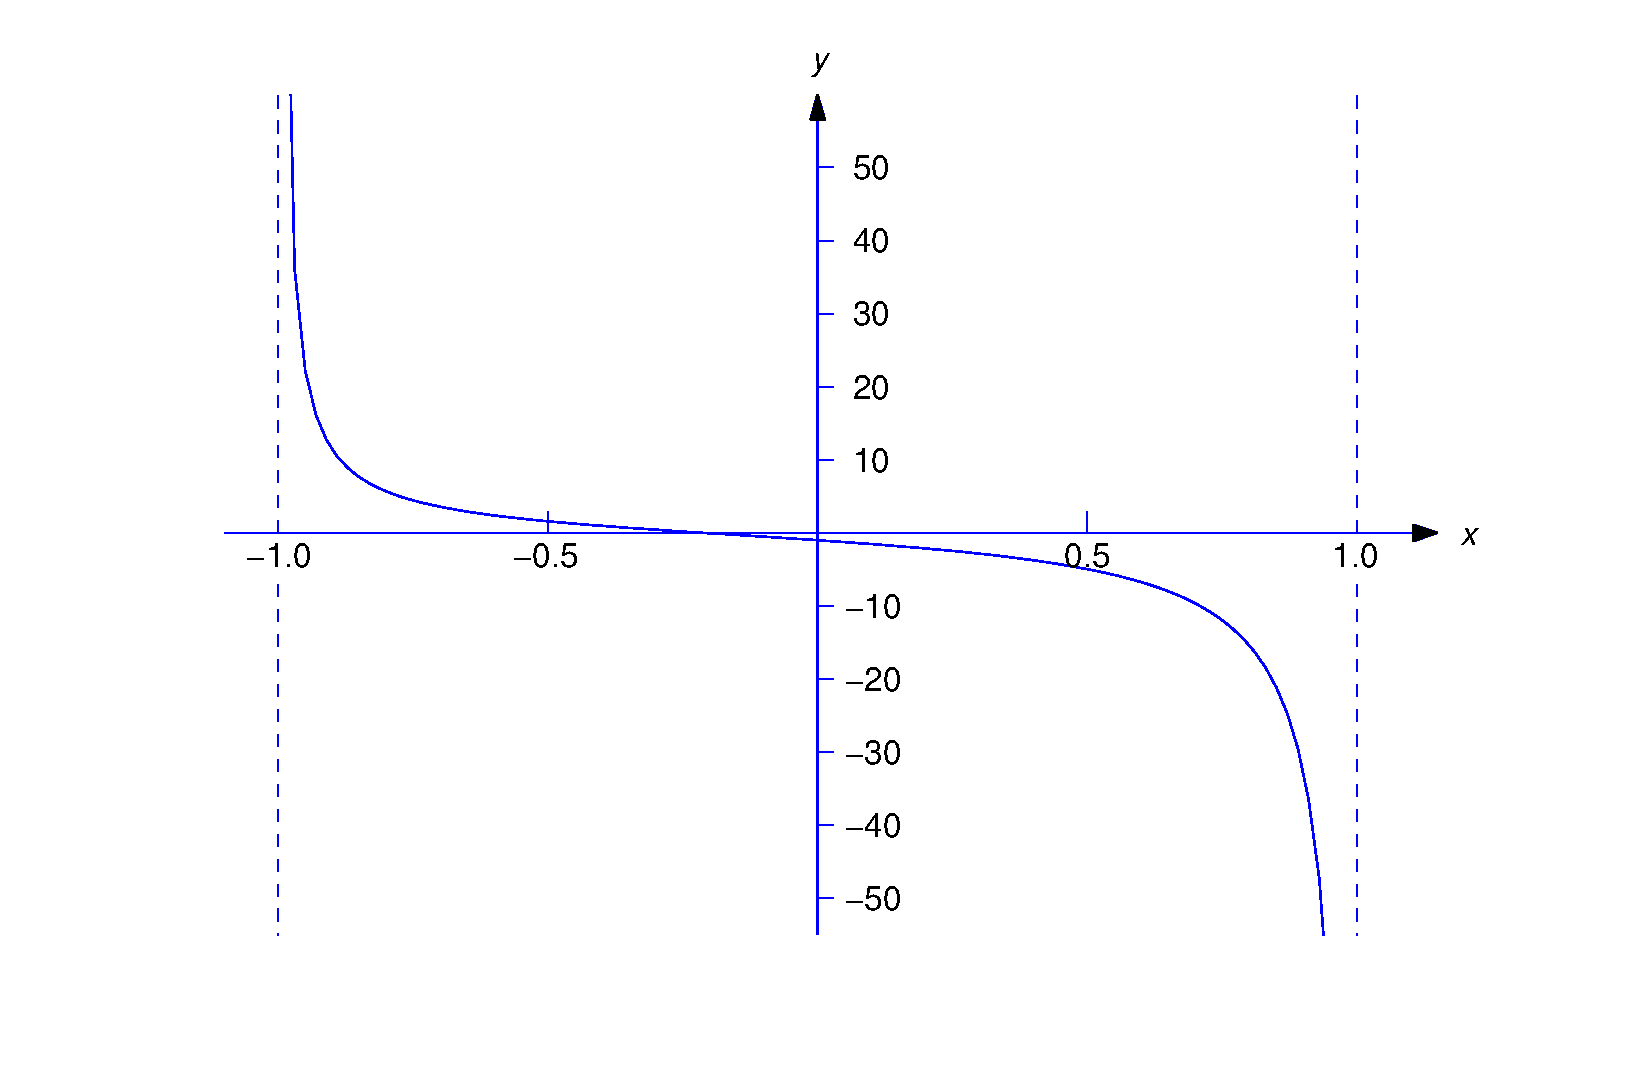
\includegraphics[bb=-78 148 689 643, width=5.67in, height=3.66in, keepaspectratio]{fig050701}
  \relax
  \caption{$y=\dst\frac{2\ln(x+1)}{x-1}+\frac{3x+1}{x^{2}-1}$}
  \label{figure:5.7.1}
\end{figure}
\end{examplesolution}

\section*{Section 6.1}
\phantomsection
\addcontentsline{toc}{chapter}{Chapter 6}
\setcounter{chapter}{6}
\setcounter{section}{1}

\setcounter{example}{0}
\begin{example}
  \label{example:6.1.1}\rm An object stretches a spring 6 inches in equilibrium.
  \begin{alist}
    \item % (a)
    Set up the equation of motion and find its general solution.

    \item % (b)
    Find the displacement of the object for $t>0$ if it's initially displaced 18 inches above
    equilibrium and given a downward velocity of 3 ft/s.
  \end{alist}
\end{example}
\setcounter{equation}{2}
\setcounter{figure}{3}
\begin{examplesolution}
\solutionpart{a} Setting $c=0$ and $F=0$ in \textup{(6.1.2)} yields the equation of motion
\[
  my''+ky=0,
\]
which we rewrite as
\begin{equation}
  \label{eq:6.1.3}y''+\frac{k}{m}y=0.
\end{equation}
Although we would need the weight of the object to obtain $k$ from the equation $mg=k\Delta l$ we
can obtain $k/m$ from $\Delta l$ alone; thus, $k/m=g/\Delta l$. Consistent with the units used in
the problem statement, we take $g=32$ ft/s$^{2}$. Although $\Delta l$ is stated in inches, we must
convert it to feet to be consistent with this choice of $g$; that is, $\Delta l=1/2$ ft. Therefore
\[
  \frac{k}{m}=\frac{32}{1/2}=64
\]
and \eqref{eq:6.1.3} becomes
\begin{equation}
  \label{eq:6.1.4}y''+64y=0.
\end{equation}
The characteristic equation of \eqref{eq:6.1.4} is
\[
  r^{2}+64=0,
\]
which has the zeros $r=\pm8i$. Therefore the general solution of \eqref{eq:6.1.4} is
\begin{equation}
  \label{eq:6.1.5}y=c_{1}\cos8t+c_{2}\sin8t.
\end{equation}

\solutionpart{b} The initial upward displacement of 18 inches is positive and must be expressed in
feet. The initial downward velocity is negative; thus,
\[
  y(0)=\frac{3}{2}\mbox{\quad and \quad}y'(0)=-3.
\]
Differentiating \eqref{eq:6.1.5} yields
\begin{equation}
  \label{eq:6.1.6}y'=-8c_{1}\sin8t+8c_{2}\cos8t.
\end{equation}
Setting $t=0$ in \eqref{eq:6.1.5} and \eqref{eq:6.1.6} and imposing the initial conditions shows
that $c_{1}=3/2$ and $c_{2}=-3/8$. Therefore
\[
  y=\frac{3}{2}\cos8t-\frac{3}{8}\sin8t,
\]
where $y$ is in feet (Figure~\ref{figure:6.1.4}).

\begin{figure}[H]
  \centering
  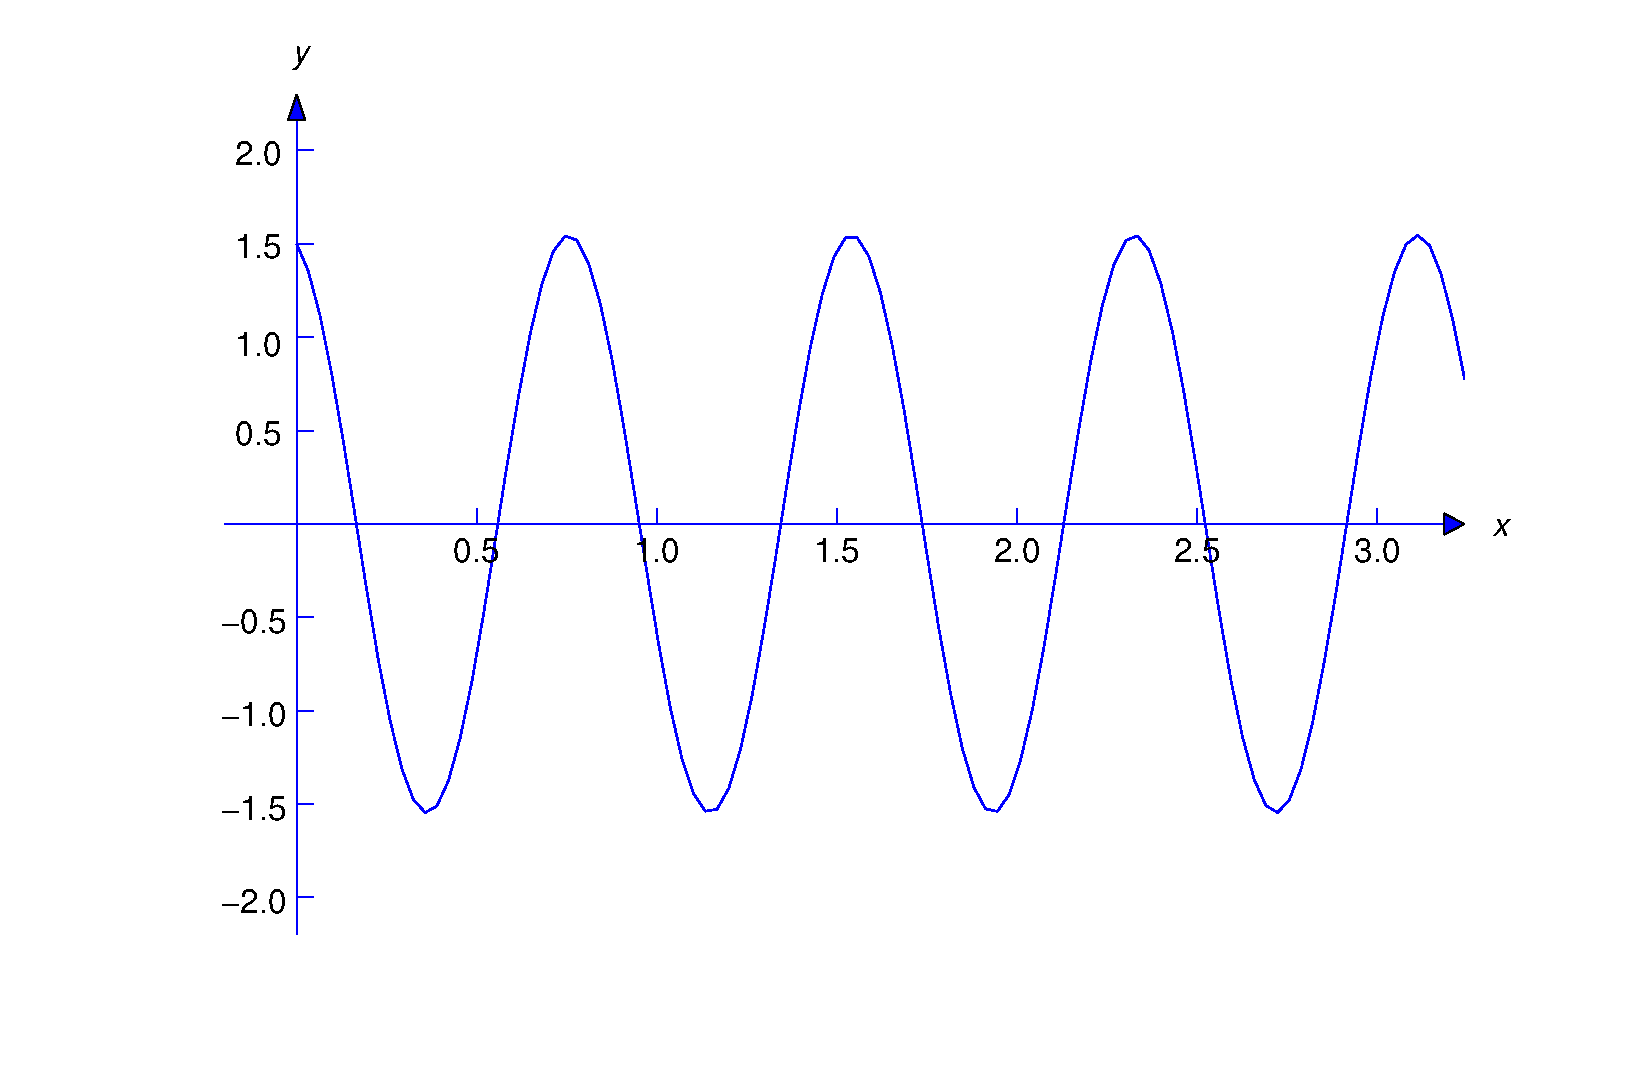
\includegraphics[bb=-78 148 689 643, width=5.67in, height=3.66in, keepaspectratio]{fig060104}
  \relax
  \caption{$y=\dst{}{\frac{3}{2}}\cos8t-\frac{3}{8}\sin8t$}
  \label{figure:6.1.4}
\end{figure}
\end{examplesolution}

\setcounter{example}{1}
\begin{example}
  \label{example:6.1.2}\rm We found the displacement of the object in Example~\ref{example:6.1.1} to
  be
  \[
    y=\frac{3}{2}\cos8t-\frac{3}{8}\sin8t.
  \]
  Find the frequency, period, amplitude, and phase angle of the motion.
\end{example}
\setcounter{equation}{10}
\begin{examplesolution}
\solution The frequency is $\omega_{0}=8$ rad/s, and the period is $T=2\pi/\omega_{0}=\pi/4$ s.
Since $c_{1}=3/2$ and $c_{2}=-3/8$, the amplitude is
\[
  R=\sqrt{c^{2}_{1}+c^{2}_{2}}=\sqrt{\left(\frac{3}{2}\right)^{2}+\left(\frac{3}{8}\right)^{2}}=\frac{3}{8}\sqrt{17}.
\]
The phase angle is determined by
\begin{equation}
  \label{eq:6.1.11}\cos\phi=\frac{\frac{3}{2}}{{\frac{3}{8}}\sqrt{17}}=\frac{4}{\sqrt{17}}
\end{equation}
and
\begin{equation}
  \label{eq:6.1.12}\sin\phi=\frac{-\frac{3}{8}}{{\frac{3}{8}}\sqrt{17}}=-\frac{1}{\sqrt{17}}.
\end{equation}
Using a calculator, we see from \eqref{eq:6.1.11} that
\[
  \phi\approx\pm.245\mbox{ rad}.
\]
Since $\sin\phi<0$ (see \eqref{eq:6.1.12}), the minus sign applies here; that is,
\[
  \phi\approx-.245\mbox{ rad}.
\]
\end{examplesolution}

\setcounter{example}{2}
\begin{example}
  \label{example:6.1.3}\rm The natural length of a spring is 1 m. An object is attached to it and
  the length of the spring increases to 102 cm when the object is in equilibrium. Then the object is
  initially displaced downward 1 cm and given an upward velocity of 14 cm/s. Find the displacement
  for $t>0$. Also, find the natural frequency, period, amplitude, and phase angle of the resulting
  motion. Express the answers in cgs units.
\end{example}
\begin{examplesolution}
\solution In cgs units $g=980$ cm/s$^{2}$. Since $\Delta l=2$ cm, $\omega_{0}^{2}=g/\Delta l=490$.
Therefore
\[
  y''+490y=0,\quad y(0)=-1,\quad y'(0)=14.
\]
The general solution of the differential equation is
\[
  y=c_{1}\cos7\sqrt{10}t+c_{2}\sin7\sqrt{10}t,
\]
so
\[
  y'=7\sqrt{10}\left(-c_{1}\sin7\sqrt{10}t+c_{2}\cos7\sqrt{10}t\right).
\]
Substituting the initial conditions into the last two equations yields $c_{1}=-1$ and
$c_{2}=2/\sqrt{10}$. Hence,
\[
  y=-\cos7\sqrt{10}t+\frac{2}{\sqrt{10}}\sin7\sqrt{10}t.
\]
The frequency is $7\sqrt{10}$ rad/s, and the period is $T=2\pi/(7\sqrt{10})$ s. The amplitude is
\[
  R=\sqrt{c_{1}^{2}+c_{2}^{2}}=\sqrt{(-1)^{2}+\left(\frac{2}{\sqrt{10}}\right)^{2}}= \sqrt{\frac{7}{5}}\mbox{ cm}.
\]
The phase angle is determined by
\[
  \cos\phi=\frac{c_{1}}{R}=-\sqrt{\frac{5}{7}}\mbox{\quad and \quad}\sin\phi= \frac{c_{2}}{R}=\sqrt{\frac{2}{7}}.
\]
Therefore $\phi$ is in the second quadrant and
\[
  \phi=\cos^{-1}\left(-\sqrt{\frac{5}{7}}\right)\approx2.58\mbox{ rad}.
\]
\end{examplesolution}

\setcounter{example}{3}
\setcounter{equation}{13}
\begin{example}
  \label{example:6.1.4}\rm Solve the initial value problem
  \begin{equation}
    \label{eq:6.1.14}y''+\omega_{0}^{2}y=\frac{F_{0}}{m}\cos\omega t,\quad y(0)=0,\quad y'(0)=0,
  \end{equation}
  given that $\omega\ne\omega_{0}$.
\end{example}
\setcounter{equation}{14}
\setcounter{figure}{5}
\begin{examplesolution}
\solution We first obtain a particular solution of \textup{(6.1.13)} by the method of undetermined
coefficients. Since $\omega\ne\omega_{0}$, $\cos\omega t$ isn't a solution of the complementary
equation
\[
  y''+\omega_{0}^{2}y=0.
\]
Therefore \textup{(6.1.13)} has a particular solution of the form
\[
  y_{p}=A\cos\omega t+B\sin\omega t.
\]
Since
\[
  y''_{p}=-\omega^{2}(A\cos\omega t+B\sin\omega t),
\]
\[
  y_{p}''+\omega_{0}^{2}y_{p}=\frac{F_{0}}{m}\cos\omega t
\]
if and only if
\[
  (\omega_{0}^{2}-\omega^{2})\left(A\cos\omega t+ B\sin\omega t\right)=\frac{F_{0}}{m}\cos\omega t.
\]
This holds if and only if
\[
  A=\frac{F_{0}}{m(\omega_{0}^{2}-\omega^{2})}\mbox{\quad and \quad}B=0,
\]
so
\[
  y_{p}=\frac{F_{0}}{m(\omega_{0}^{2}-\omega^{2})}\cos\omega t.
\]
The general solution of \textup{(6.1.13)} is
\begin{equation}
  \label{eq:6.1.15}y=\frac{F_{0}}{m(\omega_{0}^{2}-\omega^{2})}\cos\omega t +c_{1}\cos\omega_{0}t+c_{2}\sin\omega_{0}t,
\end{equation}
so
\[
  y'=\frac{-\omega F_{0}}{m(\omega_{0}^{2}-\omega^{2})}\sin\omega t +\omega_{0}(-c_{1}\sin\omega_{0}t+c_{2}\cos\omega_{0}t).
\]
The initial conditions $y(0)=0$ and $y'(0)=0$ in \eqref{eq:6.1.14} imply that
\[
  c_{1}=-\frac{F_{0}}{m(\omega_{0}^{2}-\omega^{2})}\mbox{\quad and \quad}c_{2}=0.
\]
Substituting these into \eqref{eq:6.1.15} yields
\begin{equation}
  \label{eq:6.1.16}y=\frac{F_{0}}{m(\omega_{0}^{2}-\omega^{2})}(\cos\omega t-\cos\omega_{0}t).
\end{equation}

It is revealing to write this in a different form. We start with the trigonometric identities
\begin{eqnarray*}
  \cos(\alpha-\beta) & = & \cos\alpha\cos\beta+\sin\alpha\sin\beta \\
  \cos(\alpha+\beta) & = & \cos\alpha\cos\beta-\sin\alpha\sin\beta.
\end{eqnarray*}
Subtracting the second identity from the first yields
\begin{equation}
  \label{eq:6.1.17}\cos(\alpha-\beta)-\cos(\alpha+\beta)=2\sin\alpha\sin\beta
\end{equation}
Now let
\begin{equation}
  \label{eq:6.1.18}\alpha-\beta=\omega t\mbox{\quad and \quad}\alpha+\beta=\omega_{0}t,
\end{equation}
so that
\begin{equation}
  \label{eq:6.1.19}\alpha=\frac{(\omega_{0}+\omega)t}{2}\mbox{\quad and \quad }\beta=\frac{(\omega_{0}-\omega )t}{2}.
\end{equation}
Substituting \eqref{eq:6.1.18} and \eqref{eq:6.1.19} into \eqref{eq:6.1.17} yields
\[
  \cos\omega t-\cos\omega_{0}t= 2\sin\frac{(\omega_{0}-\omega)t}{2}\sin\frac{(\omega_{0}+\omega)t}{2},
\]
and substituting this into \eqref{eq:6.1.16} yields
\begin{equation}
  \label{eq:6.1.20}y=R(t)\sin\frac{(\omega_{0}+\omega)t}{2},
\end{equation}
where
\begin{equation}
  \label{eq:6.1.21}R(t)=\frac{2F_{0}}{m(\omega_{0}^{2}-\omega^{2})}\sin\frac{(\omega_{0}-\omega)t}{2}.
\end{equation}

From \eqref{eq:6.1.20} we can regard $y$ as a sinusoidal variation with frequency
$(\omega_{0}+\omega)/2$ and variable amplitude $|R(t)|$. In Figure~\ref{figure:6.1.6} the dashed
curve above the $t$ axis is $y=|R(t)|$, the dashed curve below the $t$ axis is $y=-|R(t)|$, and the
displacement $y$ appears as an oscillation bounded by them. The oscillation of $y$ for $t$ on an
interval between successive zeros of $R(t)$ is called a {\relax\it beat\/}.

\begin{figure}[H]
  \centering
  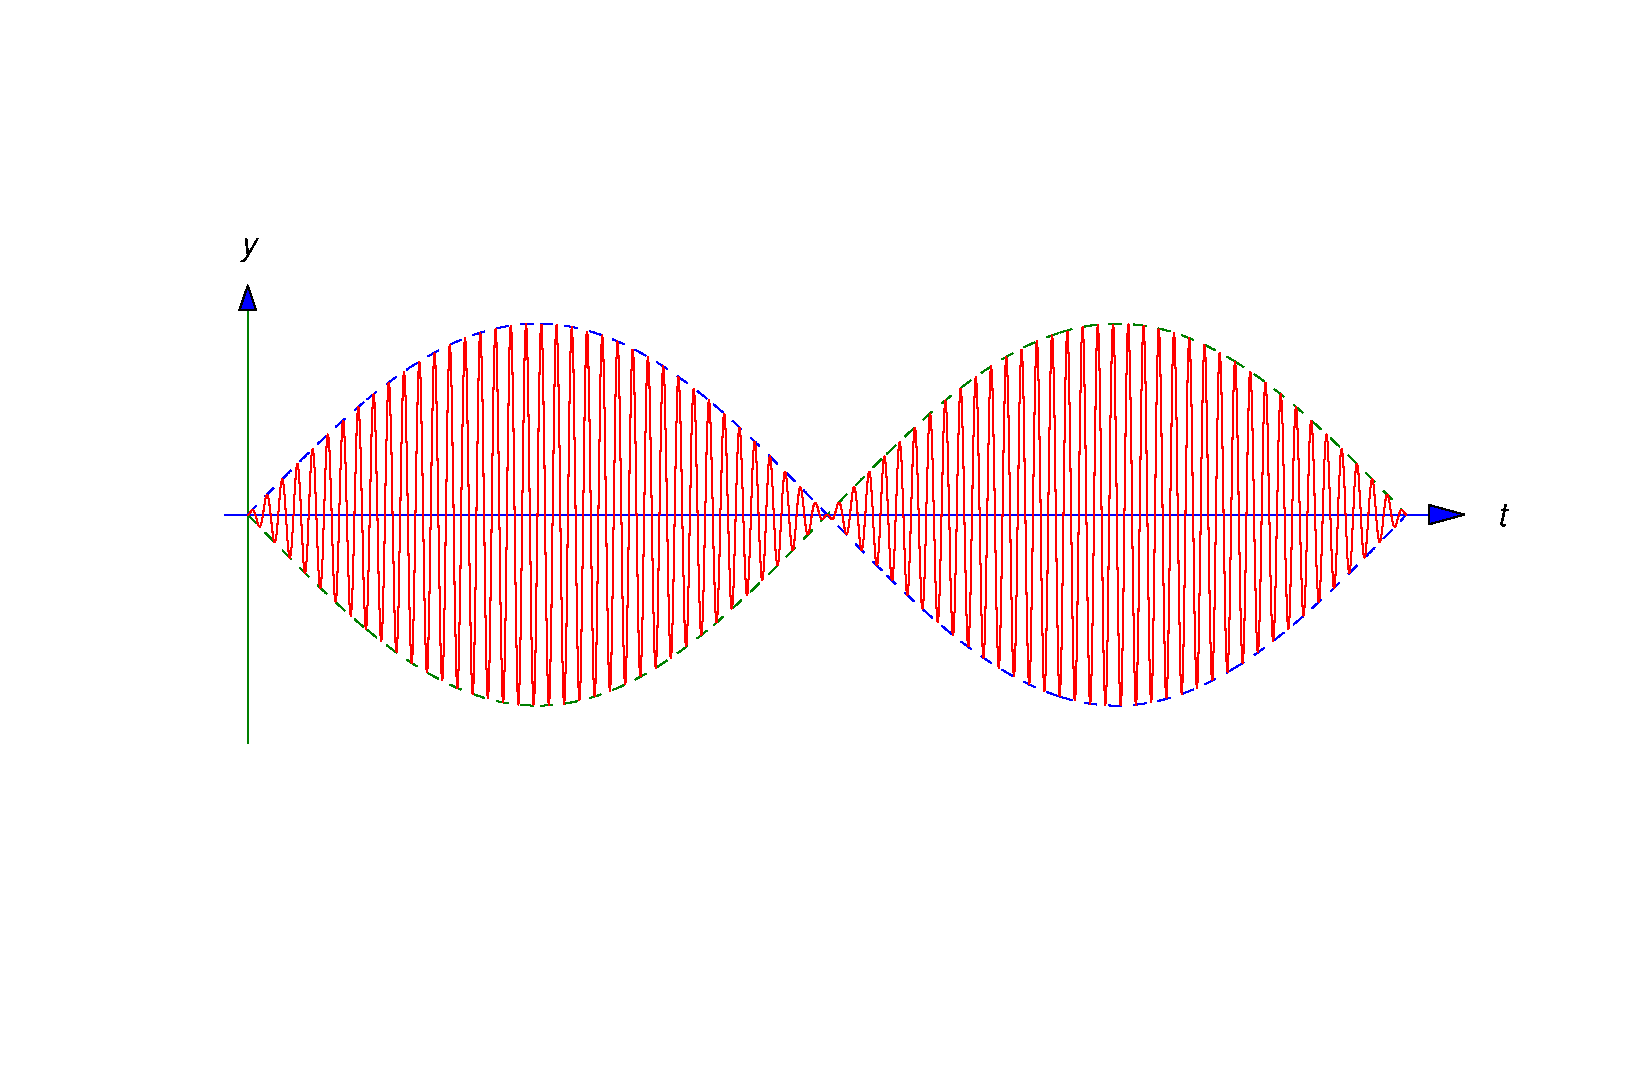
\includegraphics[bb=-78 148 689 643, width=5.67in, height=3.66in, keepaspectratio]{fig060106}
  \relax
  \caption{Undamped oscillation with beats}
  \label{figure:6.1.6}
\end{figure}

You can see from \eqref{eq:6.1.20} and \eqref{eq:6.1.21} that
\[
  |y(t)|\le\frac{2|F_{0}|}{m|\omega_{0}^{2}-\omega^{2}|};
\]
moreover, if $\omega+\omega_{0}$ is sufficiently large compared with $\omega -\omega_{0}$, then
$|y|$ assumes values close to (perhaps equal to) this upper bound during each beat. However, the
oscillation remains bounded for all $t$. (This assumes that the spring can withstand deflections of
this size and continue to obey Hooke's law.) The next example shows that this isn't so if
$\omega=\omega_{0}$.
\end{examplesolution}

\setcounter{example}{4}
\setcounter{equation}{21}
\begin{example}
  \label{example:6.1.5}\rm Find the general solution of
  \begin{equation}
    \label{eq:6.1.22}y''+\omega_{0}^{2}y=\frac{F_{0}}{m}\cos\omega_{0}t.
  \end{equation}
\end{example}
\setcounter{equation}{22}
\begin{examplesolution}
\solution We first obtain a particular solution $y_{p}$ of \eqref{eq:6.1.22}. Since
$\cos\omega_{0}t$ is a solution of the complementary equation, the form for $y_{p}$ is
\begin{equation}
  \label{eq:6.1.23}y_{p}=t(A\cos\omega_{0}t+B\sin\omega_{0}t).
\end{equation}
Then
\[
  y_{p}'=A\cos\omega_{0}t+B\sin\omega_{0}t +\omega_{0}t(-A\sin\omega_{0}t+B\cos\omega_{0}t)
\]
and
\begin{equation}
  \label{eq:6.1.24}y''_{p}=2\omega_{0}(-A\sin\omega_{0}t +B\cos\omega_{0}t)-\omega_{0}^{2}t(A\cos\omega_{0}t+B\sin\omega_{0}t).
\end{equation}
From \eqref{eq:6.1.23} and \eqref{eq:6.1.24}, we see that $y_{p}$ satisfies \eqref{eq:6.1.22} if
\[
  -2A\omega_{0}\sin\omega_{0}t+2B\omega_{0}\cos\omega_{0}t=\frac{F_{0}}{m}\cos\omega_{0}t;
\]
that is, if
\[
  A=0\mbox{\quad and \quad}B=\frac{F_{0}}{2m\omega_{0}}.
\]
Therefore
\[
  y_{p}=\frac{F_{0}t}{2m\omega_{0}}\sin\omega_{0}t
\]
is a particular solution of \eqref{eq:6.1.22}. The general solution of \eqref{eq:6.1.22} is
\[
  y=\frac{F_{0}t}{2m\omega_{0}}\sin\omega_{0}t+c_{1}\cos\omega_{0}t+c_{2}\sin\omega_{0}t.
\]
The graph of $y_{p}$ is shown in Figure~6.1.7, where it can be seen that $y_{p}$
oscillates between the dashed lines
\[
  y=\frac{F_{0}t}{2m\omega_{0}}\mbox{\quad and \quad}y=-\frac{F_{0}t}{2m\omega_{0}}
\]
with increasing amplitude that approaches $\infty$ as $t\to\infty$. Of course, this means that the
spring must eventually fail to obey Hooke's law or break.\bbox
\end{examplesolution}

\section*{Section 6.2}
\setcounter{chapter}{6}
\setcounter{section}{2}

\setcounter{example}{0}
\begin{example}
  \label{example:6.2.1}\rm Suppose a 64 lb weight stretches a spring 6 inches in equilibrium and a
  dashpot provides a damping force of $c$ lb for each ft/sec of velocity.
  \begin{alist}
    \item % (a)
    Write the equation of motion of the object and determine the value of $c$ for which the motion
    is critically damped.

    \item % (b)
    Find the displacement $y$ for $t>0$ if the motion is critically damped and the initial
    conditions are $y(0)=1$ and $y'(0)=20$.

    \item % (c)
    Find the displacement $y$ for $t>0$ if the motion is critically damped and the initial
    conditions are $y(0)=1$ and $y'(0)=-20$.
  \end{alist}
\end{example}
\setcounter{equation}{3}
\setcounter{figure}{1}
\begin{examplesolution}
\solutionpart{a} Here $m=2$ slugs and $k=64/.5=128$ lb/ft. Therefore the equation of motion
\textup{(6.2.1)} is
\begin{equation}
  \label{eq:6.2.4}2y''+cy'+128y=0.
\end{equation}
The characteristic equation is
\[
  2r^{2}+cr+128=0,
\]
which has roots
\[
  r=\frac{-c\pm\sqrt{c^{2}-8\cdot128}}{4}.
\]
Therefore the damping is critical if
\[
  c=\sqrt{8\cdot128}=32\mbox{ lb--sec/ft}.
\]

\solutionpart{b} Setting $c=32$ in \eqref{eq:6.2.4} and cancelling the common factor $2$ yields
\[
  y''+16y'+64y=0.
\]
The characteristic equation is
\[
  r^{2}+16r+64=(r+8)^{2}=0.
\]
Hence, the general solution is
\begin{equation}
  \label{eq:6.2.5}y=e^{-8t}(c_{1}+c_{2}t).
\end{equation}
Differentiating this yields
\begin{equation}
  \label{eq:6.2.6}y'=-8y+c_{2}e^{-8t}.
\end{equation}
Imposing the initial conditions $y(0)=1$ and $y'(0)=20$ in the last two equations shows that
$1=c_{1}$ and $20=-8+c_{2}$. Hence, the solution of the initial value problem is
\[
  y=e^{-8t}(1+28t).
\]
Therefore the object approaches equilibrium from above as $t\to\infty$. There's no oscillation.
\solutionpart{c} Imposing the initial conditions $y(0)=1$ and $y'(0)=-20$ in \eqref{eq:6.2.5} and
\eqref{eq:6.2.6} yields $1=c_{1}$ and $-20=-8+c_{2}$. Hence, the solution of this initial value
problem is
\[
  y=e^{-8t}(1-12t).
\]
Therefore the object moves downward through equilibrium just once, and then approaches equilibrium
from below as $t\to\infty$. Again, there's no oscillation. The solutions of these two initial value
problems are graphed in Figure~\ref{figure:6.2.2}.

\begin{figure}[H]
  \centering
  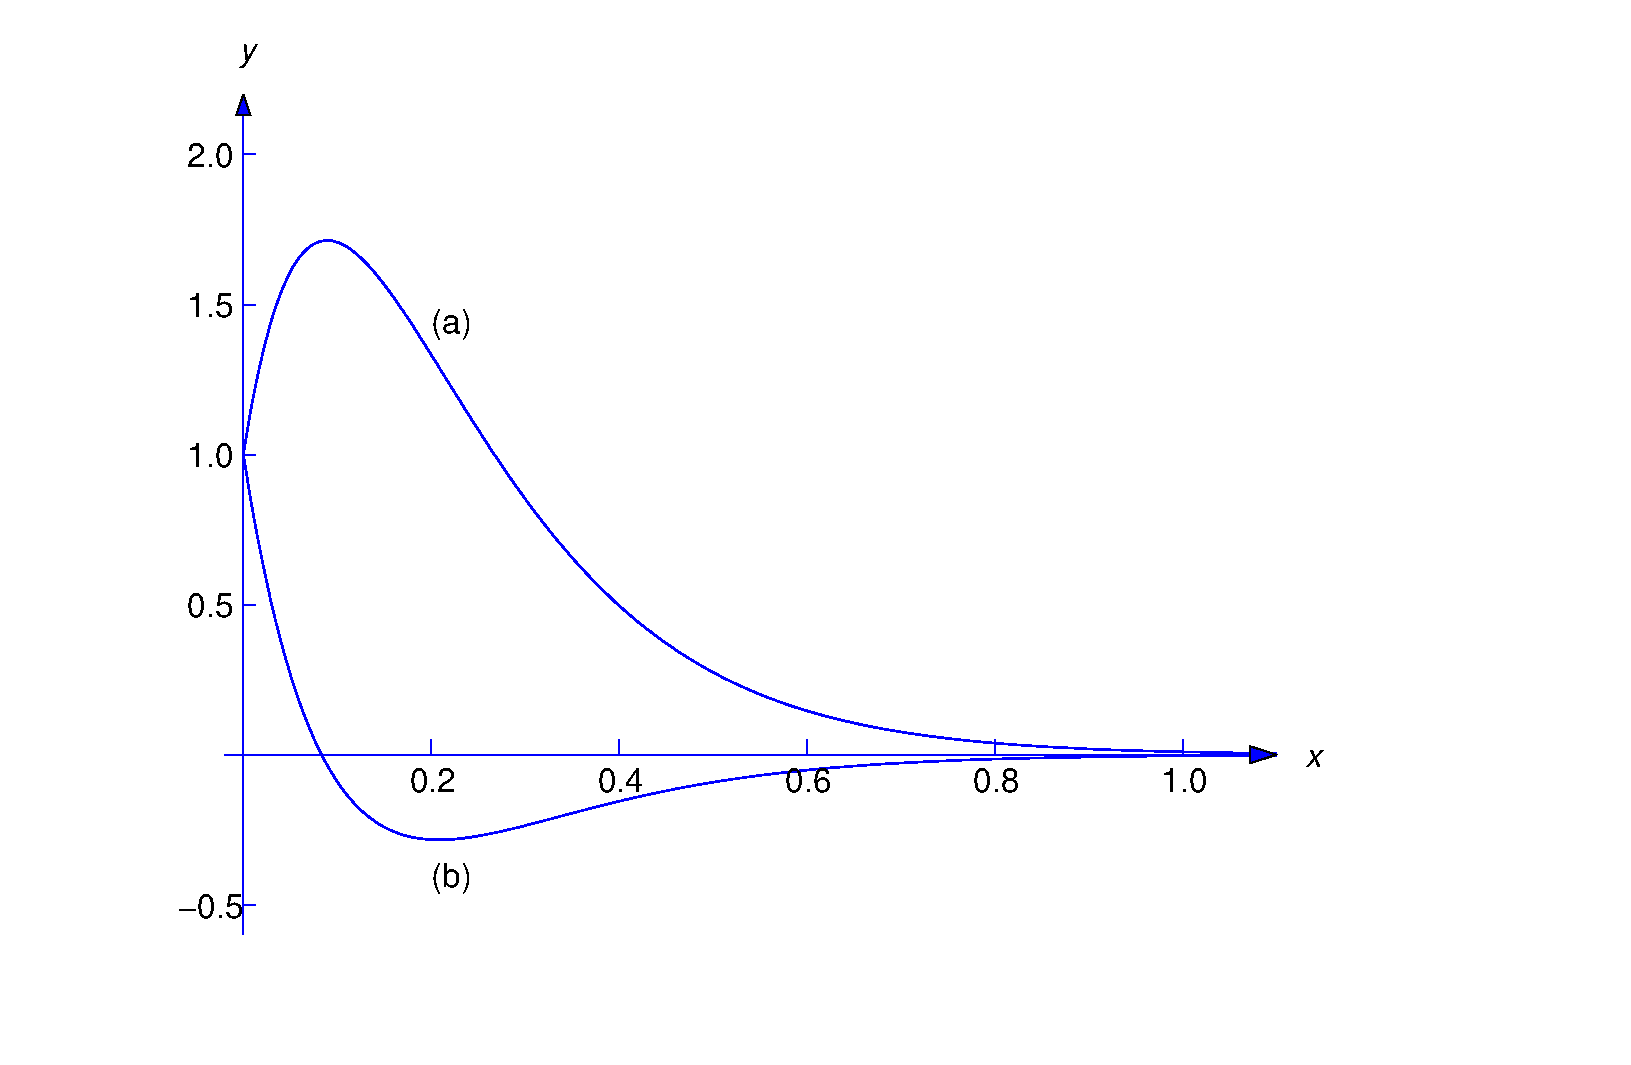
\includegraphics[bb=-78 148 689 643, width=5.67in, height=3.66in, keepaspectratio]{fig060202}
  \relax
  \caption{{\bf(a)}\, $y=e^{-8t}(1+28t)$\quad {\bf (b)}\, $y=e^{-8t}(1-12t)$}
  \label{figure:6.2.2}
\end{figure}
\end{examplesolution}

\setcounter{example}{1}
\begin{example}
  \label{example:6.2.2}\rm Find the displacement of the object in Example~\ref{example:6.2.1} if the
  damping constant is $c=4$ lb--sec/ft and the initial conditions are $y(0)=1.5$ ft and $y'(0)=-3$
  ft/sec.
\end{example}
\setcounter{equation}{6}
\begin{examplesolution}
\solution With $c=4$, the equation of motion \eqref{eq:6.2.4} becomes
\begin{equation}
  \label{eq:6.2.7}y''+2y'+64y=0
\end{equation}
after cancelling the common factor 2. The characteristic equation
\[
  r^{2}+2r+64=0
\]
has complex conjugate roots
\[
  r=\frac{-2\pm\sqrt{4-4\cdot64}}{2}=-1\pm3\sqrt{7}i.
\]
Therefore the motion is underdamped and the general solution of \eqref{eq:6.2.7} is
\[
  y=e^{-t}(c_{1}\cos3\sqrt{7}t+c_{2}\sin3\sqrt{7}t).
\]
Differentiating this yields
\[
  y'=-y+3\sqrt{7}e^{-t}(-c_{1}\sin3\sqrt{7}t+c_{2}\cos3\sqrt{7}t).
\]
Imposing the initial conditions $y(0)=1.5$ and $y'(0)=-3$ in the last two equations yields
$1.5=c_{1}$ and $-3=-1.5+3\sqrt{7}c_{2}$. Hence, the solution of the initial value problem is
\begin{equation}
  \label{eq:6.2.8}y=e^{-t}\bigg(\frac{3}{2}\cos3\sqrt{7}t-\frac{1}{2\sqrt{7}}\sin3\sqrt{7}t\bigg).
\end{equation}
The amplitude of the function in parentheses is
\[
  R=\sqrt{\bigg(\frac{3}{2}\bigg)^{2}+\bigg(\frac{1}{2\sqrt{7}}\bigg)^{2}}=\sqrt{\frac{9}{4}+\frac{1}{4\cdot7}}=\sqrt{\frac{64}{4\cdot7}}=\frac{4}{\sqrt{7}}.
\]
Therefore we can rewrite \eqref{eq:6.2.8} as
\[
  y=\frac{4}{\sqrt{7}}e^{-t}\cos(3\sqrt{7}t-\phi),
\]
where
\[
  \cos\phi=\frac{3}{2R}=\frac{3\sqrt{7}}{8}\mbox{\quad and \quad}\sin\phi=-\frac{1}{2\sqrt{7}R}= -\frac{1}{8}.
\]
Therefore $\phi\cong-.125$ radians.
\end{examplesolution}

\setcounter{example}{2}
\begin{example}
  \label{example:6.2.3}\rm Let the damping constant in Example 1 be $c=40$ lb--sec/ft. Find the
  displacement $y$ for $t>0$ if $y(0)=1$ and $y'(0)=1$.
\end{example}
\setcounter{equation}{8}
\setcounter{figure}{2}
\begin{examplesolution}
\solution With $c=40$, the equation of motion \eqref{eq:6.2.4} reduces to
\begin{equation}
  \label{eq:6.2.9}y''+20y'+64y=0
\end{equation}
after cancelling the common factor 2. The characteristic equation
\[
  r^{2}+20r+64=(r+16)(r+4)=0
\]
has the roots $r_{1}=-4$ and $r_{2}=-16$. Therefore the general solution of \eqref{eq:6.2.9} is
\begin{equation}
  \label{eq:6.2.10}y=c_{1}e^{-4t}+c_{2}e^{-16t}.
\end{equation}
Differentiating this yields
\[
  y'=-4c_{1}e^{-4t}-16c_{2}e^{-16t}.
\]
The last two equations and the initial conditions $y(0)=1$ and $y'(0)=1$ imply that
\[
  \begin{array}{rlrl}
    c_{1}   & + & c_{2}   & =1  \\
    -4c_{1} & - & 16c_{2} & =1.
  \end{array}
\]
The solution of this system is $c_{1}=17/12$, $c_{2}=-5/12$. Substituting these into
\eqref{eq:6.2.10} yields
\[
  y=\frac{17}{12}e^{-4t}-\frac{5}{12}e^{-16t}
\]
as the solution of the given initial value problem (Figure~\ref{figure:6.2.3}).

\begin{figure}[H]
  \centering
  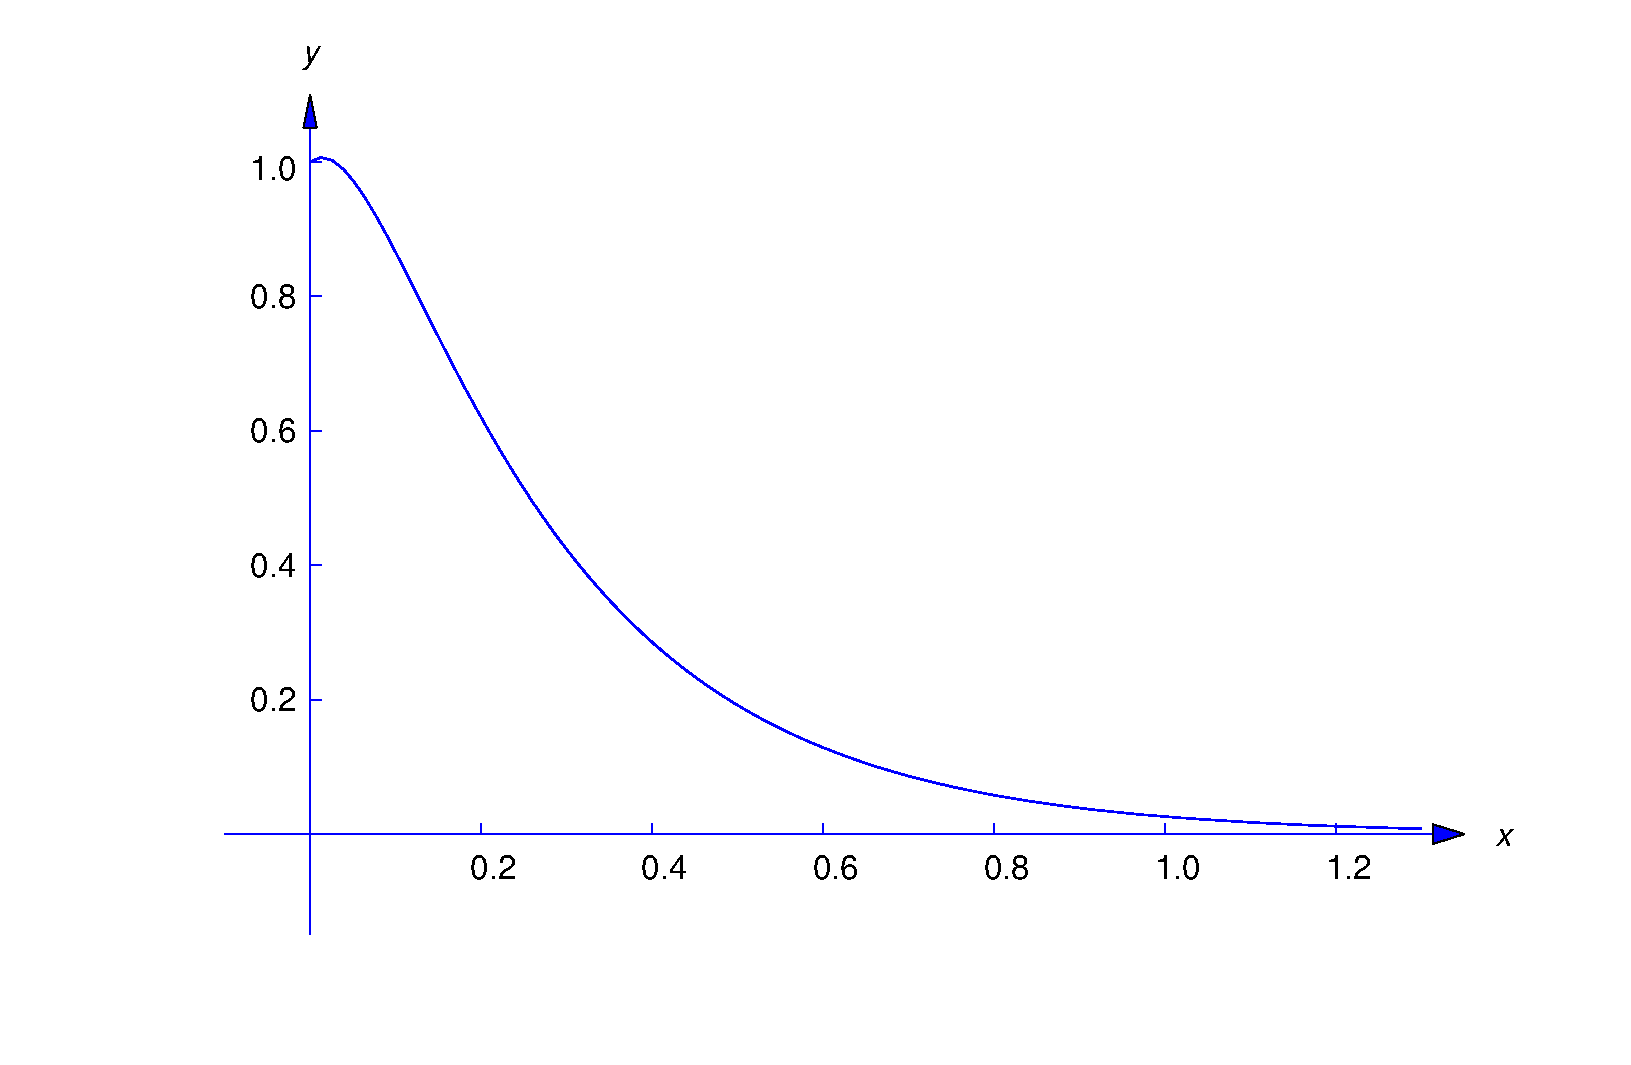
\includegraphics[bb=-78 148 689 643, width=5.67in, height=3.66in, keepaspectratio]{fig060203}
  \relax
  \caption{$y=\dst{\frac{17}{12}e^{-4t}-\frac{5}{12}e^{-16t}}$}
  \label{figure:6.2.3}
\end{figure}
\end{examplesolution}

\section*{Section 6.3}
\setcounter{chapter}{6}
\setcounter{section}{3}

\setcounter{example}{0}
\begin{example}
  \label{example:6.3.1} \rm At $t=0$ a current of 2 amperes flows in an $RLC$ circuit with
  resistance $R=40$ ohms, inductance $L=.2$ henrys, and capacitance $C=10^{-5}$ farads. Find the
  current flowing in the circuit at $t>0$ if the initial charge on the capacitor is 1 coulomb.
  Assume that $E(t)=0$ for $t>0$.
\end{example}
\setcounter{equation}{12}
\begin{examplesolution}
\solution The equation for the charge $Q$ is
\[
  \frac{1}{5}Q''+40Q'+10000Q=0,
\]
or
\begin{equation}
  \label{eq:6.3.13}Q''+200Q'+50000Q=0.
\end{equation}
Therefore we must solve the initial value problem
\begin{equation}
  \label{eq:6.3.14}Q''+200Q'+50000Q=0,\quad Q(0)=1,\quad Q'(0)=2.
\end{equation}
The desired current is the derivative of the solution of this initial value problem.

The characteristic equation of (\ref{eq:6.3.13}) is
\[
  r^{2}+200r+50000=0,
\]
which has complex zeros $r=-100\pm200i$. Therefore the general solution of (\ref{eq:6.3.13}) is
\begin{equation}
  \label{eq:6.3.15}Q=e^{-100t}(c_{1}\cos200t+c_{2}\sin200t).
\end{equation}
Differentiating this and collecting like terms yields
\begin{equation}
  \label{eq:6.3.16}Q'=-e^{-100t}\left[(100c_{1}-200c_{2})\cos200t+ (100c_{2}+200c_{1})\sin200t\right].
\end{equation}
To find the solution of the initial value problem (\ref{eq:6.3.14}), we set $t=0$ in
(\ref{eq:6.3.15}) and (\ref{eq:6.3.16}) to obtain
\[
  c_{1}=Q(0)=1\mbox{\quad and \quad}-100c_{1}+200c_{2}=Q'(0)=2;
\]
therefore, $c_{1}=1$ and $c_{2}=51/100$, so
\[
  Q=e^{-100t}\left(\cos200t+\frac{51}{100}\sin200t\right)
\]
is the solution of (\ref{eq:6.3.14}). Differentiating this yields
\[
  I=e^{-100t}(2\cos200t-251\sin200t).
\]
\end{examplesolution}

\setcounter{example}{1}
\begin{example}
  \label{example:6.3.2} \rm Find the amplitude-phase form of the steady state current in the $RLC$
  circuit in Figure~6.3.1 if the impressed voltage, provided by an alternating current
  generator, is $E(t)=E_{0}\cos\omega t$.
\end{example}
\begin{examplesolution}
\solution We'll first find the steady state charge on the capacitor as a particular solution of
\[
  LQ''+RQ'+\frac{1}{C}Q=E_{0}\cos\omega t.
\]
To do this, we'll simply reinterpret a result obtained in Section~6.2, where we found that the
steady state solution of
\[
  my''+cy'+ky=F_{0}\cos\omega t
\]
is
\[
  y_{p}=\frac{F_{0}}{\sqrt{(k-m\omega^{2})^{2}+c^{2}\omega^{2}}}\cos(\omega t-\phi),
\]
where
\[
  \cos\phi=\frac{k-m\omega^{2}}{\sqrt{(k-m\omega^{2})^{2}+c^{2}\omega^{2}}}\mbox{\quad and \quad}\sin\phi=\frac{c\omega}{\sqrt{(k-m\omega^{2})^{2}+c^{2}\omega^{2}}}.
\]
(See Equations~\textup{(6.2.14)} and \textup{(6.2.15)}.) By making the appropriate changes in the
symbols (according to Table~6.3.2) we obtain the steady state charge
\[
  Q_{p}=\frac{E_{0}}{\sqrt{(1/C-L\omega^{2})^{2}+R^{2}\omega^{2}}}\cos(\omega t-\phi),
\]
where
\[
  \cos\phi=\frac{1/C-L\omega^{2}}{\sqrt{(1/C-L\omega^{2})^{2}+R^{2}\omega^{2}}}\mbox{\quad and \quad}\sin\phi=\frac{R\omega}{\sqrt{(1/C-L\omega^{2})^{2}+R^{2}\omega^{2}}}.
\]
Therefore the steady state current in the circuit is
\[
  I_{p}=Q_{p}'= -\frac{\omega E_{0}}{\sqrt{(1/C-L\omega^{2})^{2}+R^{2}\omega^{2}}}\sin(\omega t-\phi).
\]
\end{examplesolution}

\section*{Section 7.1}
\phantomsection
\addcontentsline{toc}{chapter}{Chapter 7}
\setcounter{chapter}{7}
\setcounter{section}{1}

\setcounter{example}{0}
\begin{example}
  \label{example:7.1.1} \rm Find the radius of convergence of the series:
  \[
    \mbox{\bf (a)}\quad\sum_{n=0}^{\infty}n!x^{n}\quad\mbox{\bf (b) }\quad \sum_{n=10}^{\infty}(-1)^{n}\frac{x^{n}}{n!}\quad\mbox{\bf (c) }\quad \sum_{n=0}^{\infty}2^{n}n^{2}(x-1)^{n}.
  \]
\end{example}
\begin{examplesolution}
\solutionpart{a} Here $a_{n}=n!$, so
\[
  \lim_{n\to\infty}\left|\frac{a_{n+1}}{a_{n}}\right|=\lim_{n\to\infty}\frac{(n+1)!}{n!}=\lim_{n\to\infty}(n+1)=\infty.
\]
Hence, $R=0$.

\solutionpart{b} Here $a_{n}=(-1)^{n}/n!$ for $n\ge N=10$, so
\[
  \lim_{n\to\infty}\left|\frac{a_{n+1}}{a_{n}}\right|=\lim_{n\to\infty}\frac{n!}{(n+1)!}=\lim_{n\to\infty}\frac{1}{n+1}=0.
\]
Hence, $R=\infty$.

\solutionpart{c} Here $a_{n}=2^{n}n^{2}$, so
\[
  \lim_{n\to\infty}\left|\frac{a_{n+1}}{a_{n}}\right|=\lim_{n\to\infty}\frac{2^{n+1}(n+1)^{2}}{2^{n}n^{2}}=2\lim_{n\to\infty}\left(1+\frac{1}{n}\right)^{2}=2.
\]
Hence, $R=1/2$.
\end{examplesolution}

\setcounter{example}{1}
\begin{example}
  \label{example:7.1.2} \rm Let $f(x)=\sin x$. From \textup{(7.1.3)},
  \[
    f(x)=\sum_{n=0}^{\infty}(-1)^{n}\frac{x^{2n+1}}{(2n+1)!}.
  \]
  From \textup{(7.1.6)},
  \[
    f'(x)=\sum_{n=0}^{\infty}(-1)^{n}\frac{d}{dx}\left[\frac{x^{2n+1}}{(2n+1)!}\right]= \sum_{n=0}^{\infty}(-1)^{n}\frac{x^{2n}}{(2n)!},
  \]
  which is the series \textup{(7.1.4)} for $\cos x$.
\end{example}

\setcounter{example}{2}
\begin{example}
  \label{example:7.1.3} \rm Rewrite the following power series from \textup{(7.1.7)} and
  \textup{(7.1.8)} so that the general term in each is a constant multiple of $(x-x_{0})^{n}$:
  \[
    \mbox{\bf (a)}\; \sum_{n=2}^{\infty}n(n-1)a_{n}(x-x_{0})^{n-2}\quad\mbox{\bf (b)}\; \sum_{n=k}^{\infty}n(n-1)\cdots(n-k+1)a_{n}(x-x_{0})^{n-k}.
  \]
\end{example}
\begin{examplesolution}
\solutionpart{a} Replacing $n$ by $n+2$ in the general term and subtracting $2$ from the lower limit
of summation yields
\[
  \sum_{n=2}^{\infty}n(n-1)a_{n}(x-x_{0})^{n-2}= \sum_{n=0}^{\infty}(n+2)(n+1)a_{n+2}(x-x_{0})^{n}.
\]

\solutionpart{b} Replacing $n$ by $n+k$ in the general term and subtracting $k$ from the lower limit
of summation yields
\[
  \sum_{n=k}^{\infty}n(n-1)\cdots(n-k+1)a_{n}(x-x_{0})^{n-k}= \sum_{n=0}^{\infty}(n+k)(n+k-1)\cdots(n+1)a_{n+k}(x-x_{0})^{n}.
\]
\end{examplesolution}

\setcounter{example}{3}
\begin{example}
  \label{example:7.1.4} \rm Given that
  \[
    f(x)=\sum_{n=0}^{\infty}a_{n}x^{n},
  \]
  write the function $xf''$ as a power series in which the general term is a constant multiple
  of~$x^{n}$.
\end{example}
\begin{examplesolution}
\solution From Theorem~7.1.4 with $x_{0}=0$,
\[
  f''(x)=\sum_{n=2}^{\infty}n(n-1)a_{n}x^{n-2}.
\]
Therefore
\[
  xf''(x)=\sum_{n=2}^{\infty}n(n-1)a_{n}x^{n-1}.
\]
Replacing $n$ by $n+1$ in the general term and subtracting $1$ from the lower limit of summation
yields
\[
  xf''(x)=\sum_{n=1}^{\infty}(n+1)na_{n+1}x^{n}.
\]
We can also write this as
\[
  xf''(x)=\sum_{n=0}^{\infty}(n+1)na_{n+1}x^{n},
\]
since the first term in this last series is zero. (We'll see later that sometimes it's useful to
include zero terms at the beginning of a series.)
\end{examplesolution}

\setcounter{example}{4}
\begin{example}
  \label{example:7.1.5} \rm Find the Maclaurin series for $\cosh x$ as a linear combination of the
  Maclaurin series for $e^{x}$ and $e^{-x}$.
\end{example}
\setcounter{equation}{11}
\begin{examplesolution}
\solution By definition,
\[
  \cosh x=\frac{1}{2}e^{x}+\frac{1}{2}e^{-x}.
\]
Since
\[
  e^{x}=\sum_{n=0}^{\infty}\frac{x^{n}}{n!}\quad\mbox{ and }\quad e^{-x}=\sum_{n=0}^{\infty}(-1)^{n}\frac{x^{n}}{n!},
\]
it follows that
\begin{equation}
  \label{eq:7.1.12}\cosh x=\sum_{n=0}^{\infty}\frac{1}{2}[1+(-1)^{n}]{\frac{x^{n}}{n!}}.
\end{equation}
Since
\[
  \frac{1}{2}[1+(-1)^{n}]=\left\{
  \begin{array}{cl}
    1 & \mbox{ if }n=2m,\mbox{ an even integer},  \\
    0 & \mbox{ if }n=2m+1,\mbox{ an odd integer},
  \end{array}\right.
\]
we can rewrite \eqref{eq:7.1.12} more simply as
\[
  \cosh x=\sum_{m=0}^{\infty}\frac{x^{2m}}{(2m)!}.
\]
This result is valid on $(-\infty,\infty)$, since this is the open interval of convergence of the
Maclaurin series for $e^{x}$ and $e^{-x}$.
\end{examplesolution}

\setcounter{example}{5}
\setcounter{equation}{12}
\begin{example}
  \label{example:7.1.6} \rm Suppose
  \[
    y=\sum_{n=0}^{\infty}a_{n}x^{n}
  \]
  on an open interval $I$ that contains the origin.
  \begin{alist}
    \item % (a)
    Express
    \[
      (2-x)y''+2y
    \]
    as a power series in $x$ on $I$.

    \item % (b)
    Use the result of \part{a} to find necessary and sufficient conditions on the coefficients
    $\{a_{n}\}$ for $y$ to be a solution of the homogeneous equation
    \begin{equation}
      \label{eq:7.1.13}(2-x)y''+2y=0
    \end{equation}
    on $I$.
  \end{alist}
\end{example}
\setcounter{equation}{13}
\begin{examplesolution}
\solutionpart{a} From \textup{(7.1.7)} with $x_{0}=0$,
\[
  y''=\sum_{n=2}^{\infty}n(n-1)a_{n}x^{n-2}.
\]
Therefore
\begin{equation}
  \label{eq:7.1.14}
  \begin{array}{rcl}
    (2-x)y''+2y & = & 2y''-xy''+2y                                                                                                          \\[\jot]
                & = & \dst{\sum_{n=2}^{\infty}2n(n-1)a_{n}x^{n-2} -\sum_{n=2}^{\infty}n(n-1)a_{n}x^{n-1} +\sum_{n=0}^{\infty}2a_{n}x^{n}}.
  \end{array}
\end{equation}
To combine the three series we shift indices in the first two to make their general terms constant
multiples of $x^{n}$; thus,
\begin{equation}
  \label{eq:7.1.15}\sum_{n=2}^{\infty}2n(n-1)a_{n}x^{n-2}=\sum_{n=0}^{\infty}2(n+2)(n+1)a_{n+2}x^{n}
\end{equation}
and
\begin{equation}
  \label{eq:7.1.16}\sum_{n=2}^{\infty}n(n-1)a_{n}x^{n-1}=\sum_{n=1}^{\infty}(n+1)na_{n+1}x^{n}=\sum_{n=0}^{\infty}(n+1)na_{n+1}x^{n},
\end{equation}
where we added a zero term in the last series so that when we substitute from \eqref{eq:7.1.15} and
\eqref{eq:7.1.16} into \eqref{eq:7.1.14} all three series will start with $n=0$; thus,
\begin{equation}
  \label{eq:7.1.17}(2-x)y''+2y=\sum_{n=0}^{\infty}[2(n+2)(n+1)a_{n+2}-(n+1)na_{n+1}+2a_{n}]x^{n}.
\end{equation}

\solutionpart{b} From \eqref{eq:7.1.17} we see that $y$ satisfies \eqref{eq:7.1.13} on $I$ if
\begin{equation}
  \label{eq:7.1.18}2(n+2)(n+1)a_{n+2}-(n+1)na_{n+1}+2a_{n}=0,\quad n=0,1,2,\dots.
\end{equation}
Conversely, Theorem~7.1.6~\part{b} implies that if $y=\sum_{n=0}^{\infty}a_{n}x^{n}$
satisfies \eqref{eq:7.1.13} on $I$, then \eqref{eq:7.1.18} holds.
\end{examplesolution}

\setcounter{example}{6}
\setcounter{equation}{18}
\begin{example}
  \label{example:7.1.7} \rm Suppose
  \[
    y=\sum_{n=0}^{\infty}a_{n}(x-1)^{n}
  \]
  on an open interval $I$ that contains $x_{0}=1$. Express the function
  \begin{equation}
    \label{eq:7.1.19}(1+x)y''+2(x-1)^{2}y'+3y
  \end{equation}
  as a power series in $x-1$ on $I$.
\end{example}
\setcounter{equation}{19}
\begin{examplesolution}
\solution Since we want a power series in $x-1$, we rewrite the coefficient of $y''$ in
\eqref{eq:7.1.19} as $1+x=2+(x-1)$, so \eqref{eq:7.1.19} becomes
\[
  2y''+(x-1)y''+2(x-1)^{2}y'+3y.
\]
From \textup{(7.1.6)} and \textup{(7.1.7)} with $x_{0}=1$,
\[
  y'=\sum_{n=1}^{\infty}na_{n}(x-1)^{n-1}\quad\mbox{ and }\quad y''=\sum_{n=2}^{\infty}n(n-1)a_{n}(x-1)^{n-2}.
\]
Therefore
\begin{eqnarray*}
  2y''         & = & \sum_{n=2}^{\infty}2n(n-1)a_{n}(x-1)^{n-2}, \\
  (x-1)y''     & = & \sum_{n=2}^{\infty}n(n-1)a_{n}(x-1)^{n-1},  \\
  2(x-1)^{2}y' & = & \sum_{n=1}^{\infty}2na_{n}(x-1)^{n+1},      \\
  3y           & = & \sum_{n=0}^{\infty}3a_{n}(x-1)^{n}.
\end{eqnarray*}
Before adding these four series we shift indices in the first three so that their general terms
become constant multiples of $(x-1)^{n}$. This yields
\begin{eqnarray}
  2y ''&=&\sum_{n=0}^\infty 2(n+2)(n+1)a_{n+2}(x-1)^n,\label{eq:7.1.20}\\ (x-1)y''&=&\sum_{n=0}^\infty (n+1)na_{n+1}(x-1)^n, \label{eq:7.1.21}\\ 2(x-1)^2y'&=&\sum_{n=1}^\infty 2(n-1)a_{n-1}(x-1)^n,\label{eq:7.1.22}\\
  %dummy \eqref{eq:7.1.22}
  3y&=&\sum_{n=0}^\infty 3a_n (x-1)^n, \label{eq:7.1.23}
\end{eqnarray}
where we added initial zero terms to the series in \eqref{eq:7.1.21} and \eqref{eq:7.1.22}. Adding
\eqref{eq:7.1.20}--\eqref{eq:7.1.23} yields
\begin{eqnarray*}
  (1+x)y''+2(x-1)^{2}y'+3y & = & 2y''+(x-1)y''+2(x-1)^{2}y'+3y \\[5pt]
                           & = & \sum_{n=0}^{\infty}b_{n}(x-1)^{n},
\end{eqnarray*}
where
\begin{eqnarray}
  b_{0} & = & 4a_{2}+3a_{0},\label{eq:7.1.24} \\
  b_{n} & = & 2(n+2)(n+1)a_{n+2}+(n+1)na_{n+1}+2(n-1)a_{n-1}+3a_{n},\,n\ge1\label{eq:7.1.25}.
\end{eqnarray}
The formula \eqref{eq:7.1.24} for $b_{0}$ can't be obtained by setting $n=0$ in \eqref{eq:7.1.25},
since the summation in \eqref{eq:7.1.22} begins with $n=1$, while those in \eqref{eq:7.1.20},
\eqref{eq:7.1.21}, and \eqref{eq:7.1.23} begin with $n=0$.
\end{examplesolution}

\section*{Section 7.2}
\setcounter{chapter}{7}
\setcounter{section}{2}

\setcounter{example}{0}
\setcounter{equation}{8}
\begin{example}
  \label{example:7.2.1}\rm Let $x_{0}$ be an arbitrary real number. Find the power series in
  $x-x_{0}$ for the general solution of
  \begin{equation}
    \label{eq:7.2.9}y''+y=0.
  \end{equation}
\end{example}
\setcounter{equation}{9}
\begin{examplesolution}
\solution Here
\[
  Ly=y''+y.
\]
If
\[
  y=\sum_{n=0}^{\infty}a_{n}(x-x_{0})^{n},
\]
then
\[
  y''=\sum_{n=2}^{\infty}n(n-1)a_{n}(x-x_{0})^{n-2},
\]
so
\[
  Ly=\sum_{n=2}^{\infty}n(n-1)a_{n}(x-x_{0})^{n-2}+\sum_{n=0}^{\infty}a_{n}(x-x_{0})^{n}.
\]
To collect coefficients of like powers of $x-x_{0}$, we shift the summation index in the first sum.
This yields
\[
  Ly=\sum^{\infty}_{n=0}(n+2)(n+1)a_{n+2}(x-x_{0})^{n}+ \sum^{\infty}_{n=0}a_{n}(x-x_{0})^{n}=\sum^{\infty}_{n=0}b_{n}(x-x_{0})^{n},
\]
with
\[
  b_{n}=(n+2)(n+1)a_{n+2}+a_{n}.
\]
Therefore $Ly=0$ if and only if
\begin{equation}
  \label{eq:7.2.10}a_{n+2}=\frac{-a_{n}}{(n+2)(n+1)},\quad n\ge0,
\end{equation}
where $a_{0}$ and $a_{1}$ are arbitrary. Since the indices on the left and right sides of
\eqref{eq:7.2.10} differ by two, we write \eqref{eq:7.2.10} separately for $n$ even $(n=2m)$ and $n$
odd $(n=2m+1)$. This yields
\begin{eqnarray}
  a_{2m+2}&=&\frac{-a_{2m}}{(2m+2)(2m+1)},\quad m\ge0, \label{eq:7.2.11} \\%dummy \eqref{eq:7.2.14}
  \noalign{\hspace*{-15pt}\mbox{and}}\nonumber\\ a_{2m+3}&=&\frac{-a_{2m+1}}{(2m+3)(2m+2)},\quad m\ge0. \label{eq:7.2.12}
\end{eqnarray}
Computing the coefficients of the even powers of $x-x_{0}$ from \eqref{eq:7.2.11} yields
\begin{eqnarray*}
  a_{2} & = & -\frac{a_{0}}{2\cdot1}                                                                                          \\[2\jot]
  a_{4} & = & -\frac{a_{2}}{4\cdot3}=-\frac{1}{4\cdot3}\left(-\frac{a_{0}}{2\cdot1}\right)=\frac{a_{0}}{4\cdot3\cdot2\cdot1}, \\
  a_{6} & = & -\frac{a_{4}}{6\cdot5}=-\frac{1}{6\cdot5}\left(\frac{a_{0}}{4\cdot3\cdot2\cdot1}\right)=-\frac{a_{0}}{6\cdot5\cdot4\cdot3\cdot2\cdot1},
\end{eqnarray*}
and, in general,
\begin{equation}
  \label{eq:7.2.13}a_{2m}=(-1)^{m}\frac{a_{0}}{(2m)!}\;,\quad m\ge0.
\end{equation}
Computing the coefficients of the odd powers of $x-x_{0}$ from \eqref{eq:7.2.12} yields
\begin{eqnarray*}
  a_{3} & = & -\frac{a_{1}}{3\cdot2}                                                                                          \\[2\jot]
  a_{5} & = & -\frac{a_{3}}{5\cdot4}=-\frac{1}{5\cdot4}\left(-\frac{a_{1}}{3\cdot2}\right)=\frac{a_{1}}{5\cdot4\cdot3\cdot2}, \\
  a_{7} & = & -\frac{a_{5}}{7\cdot6}=-\frac{1}{7\cdot6}\left(\frac{a_{1}}{5\cdot4\cdot3\cdot2}\right)=-\frac{a_{1}}{7\cdot6\cdot5\cdot4\cdot3\cdot2},
\end{eqnarray*}
and, in general,
\begin{equation}
  \label{eq:7.2.14}a_{2m+1}=\frac{(-1)^{m}a_{1}}{(2m+1)!}\quad m\ge0.
\end{equation}
Thus, the general solution of \eqref{eq:7.2.9} can be written as
\[
  y=\sum_{m=0}^{\infty}a_{2m}(x-x_{0})^{2m}+\sum_{m=0}^{\infty}a_{2m+1}(x-x_{0})^{2m+1},
\]
or, from \eqref{eq:7.2.13} and \eqref{eq:7.2.14}, as
\begin{equation}
  \label{eq:7.2.15}y=a_{0}\sum_{m=0}^{\infty}(-1)^{m}\frac{(x-x_{0})^{2m}}{(2m)!}+a_{1}\sum_{m=0}^{\infty}(-1)^{m}\frac{(x-x_{0})^{2m+1}}{(2m+1)!}.
\end{equation}
If we recall from calculus that
\[
  \sum_{m=0}^{\infty}(-1)^{m}\frac{(x-x_{0})^{2m}}{(2m)!}=\cos(x-x_{0}) \mbox{\quad and \quad }\sum_{m=0}^{\infty}(-1)^{m}\frac{(x-x_{0})^{2m+1}}{(2m+1)!}=\sin(x-x_{0}),
\]
then \eqref{eq:7.2.15} becomes
\[
  y=a_{0}\cos(x-x_{0})+a_{1}\sin(x-x_{0}),
\]
which should look familiar. \bbox
\end{examplesolution}

\setcounter{example}{1}
\setcounter{equation}{16}
\begin{example}
  \label{example:7.2.2}\rm Find the power series in $x$ for the general solution of
  \begin{equation}
    \label{eq:7.2.17}(1+2x^{2})y''+6xy'+2y=0.
  \end{equation}
\end{example}
\setcounter{equation}{17}
\begin{examplesolution}
\solution Here
\[
  Ly=(1+2x^{2})y''+6xy'+2y.
\]
If
\[
  y=\sum_{n=0}^{\infty}a_{n}x^{n}
\]
then
\[
  y'=\sum_{n=1}^{\infty}na_{n}x^{n-1}\quad\mbox{ and }\quad y''=\sum_{n=2}^{\infty}n(n-1)a_{n}x^{n-2},
\]
so
\begin{eqnarray*}
  Ly & = & (1+2x^{2})\sum^{\infty}_{n=2}n(n-1)a_{n}x^{n-2}+6x\sum^{\infty}_{n=1}na_{n}x^{n-1}+2\sum^{\infty}_{n=0}a_{n}x^{n} \\[2\jot]
     & = & \sum_{n=2}^{\infty}n(n-1)a_{n}x^{n-2}+\sum_{n=0}^{\infty}\left[2n(n-1)+6n+2\right]a_{n}x^{n}                      \\[2\jot]
     & = & \sum_{n=2}^{\infty}n(n-1)a_{n}x^{n-2}+2\sum_{n=0}^{\infty}(n+1)^{2}a_{n}x^{n}.
\end{eqnarray*}
To collect coefficients of $x^{n}$, we shift the summation index in the first sum. This yields
\[
  Ly=\sum_{n=0}^{\infty}(n+2)(n+1)a_{n+2}x^{n}+2\sum_{n=0}^{\infty}(n+1)^{2}a_{n}x^{n}=\sum_{n=0}^{\infty}b_{n}x^{n},
\]
with
\[
  b_{n}=(n+2)(n+1)a_{n+2}+2(n+1)^{2}a_{n},\quad n\ge0.
\]
To obtain solutions of \eqref{eq:7.2.17}, we set $b_{n}=0$ for $n\ge0$. This is equivalent to the
recurrence relation
\begin{equation}
  \label{eq:7.2.18}a_{n+2}=-2{\frac{n+1}{n+2}}a_{n},\quad n\ge0.
\end{equation}
Since the indices on the left and right differ by two, we write \eqref{eq:7.2.18} separately for
$n=2m$ and $n=2m+1$, as in Example~\ref{example:7.2.1}. This yields
\begin{eqnarray}
  a_{2m+2}                                     & = & -2{\frac{2m+1}{2m+2}}a_{2m}=-\frac{2m+1}{m+1}a_{2m},\quad m\ge0,\label{eq:7.2.19} \\
  \noalign{\hspace*{-15pt}\mbox{and}}\nonumber                                                                                         \\
  a_{2m+3}                                     & = & -2{\frac{2m+2}{2m+3}}a_{2m+1}=-4{\frac{m+1}{2m+3}}a_{2m+1},\quad m\ge0.\label{eq:7.2.20}
\end{eqnarray}
Computing the coefficients of even powers of $x$ from \eqref{eq:7.2.19} yields
\begin{eqnarray*}
  a_{2}&=&-\frac{1}{1}a_{0},\\[5pt] a_{4}&=&-\frac{3}{2}a_{2}=\left(-\frac{3}{2}\right)\left(-\frac{1}{1}\right)a_{0} =\frac{1\cdot3}{1\cdot2}a_{0}, \\[5pt]a_{6}&=&-\frac{5}{3}a_{4}= -\frac{5}{3}\left(\frac{1\cdot3}{1\cdot2}\right)a_{0} =-\frac{1\cdot3\cdot5}{1\cdot2\cdot3}a_{0},\\[5pt] a_{8}&=&-\frac{7}{4}a_{6}=-\frac{7}{4} \left(-\frac{1\cdot3\cdot5}{1\cdot2\cdot3}\right)a_{0}= \frac{1\cdot3\cdot5\cdot7}{1\cdot2\cdot3\cdot4}a_{0}.\\
\end{eqnarray*}
In general,
\begin{equation}
  \label{eq:7.2.21}a_{2m}=(-1)^{m}\frac{\prod_{j=1}^{m}(2j-1)}{m!}a_{0},\quad m\ge0.
\end{equation}
(Note that \eqref{eq:7.2.21} is correct for $m=0$ because we defined $\prod_{j=1}^{0}b_{j}=1$ for
any~$b_{j}$.)

Computing the coefficients of odd powers of $x$ from \eqref{eq:7.2.20} yields
\begin{eqnarray*}
  a_{3} & = & -4\,\frac{1}{3}a_{1},                                                                                                              \\[5pt]
  a_{5} & = & -4\,\frac{2}{5}a_{3}=-4\,\frac{2}{5}\left(-4{\frac{1}{3}}\right)a_{1}=4^{2}\frac{1\cdot2}{3\cdot5}a_{1},                           \\[5pt]
  a_{7} & = & -4\,\frac{3}{7}a_{5}=-4\,\frac{3}{7}\left(4^{2}\frac{1\cdot2}{3\cdot5}\right)a_{1}=-4^{3}\frac{1\cdot2\cdot3}{3\cdot5\cdot7}a_{1}, \\[5pt]
  a_{9} & = & -4\,\frac{4}{9}a_{7}=-4\,\frac{4}{9}\left(4^{3}\frac{1\cdot2\cdot3}{3\cdot5\cdot7}\right)a_{1}=4^{4}\frac{1\cdot2\cdot3\cdot4}{3\cdot5\cdot7\cdot9}a_{1}.
\end{eqnarray*}
In general,
\begin{equation}
  \label{eq:7.2.22}a_{2m+1}=\frac{(-1)^{m}4^{m}m!}{\prod_{j=1}^{m}(2j+1)}a_{1},\quad m\ge0.
\end{equation}
From \eqref{eq:7.2.21} and \eqref{eq:7.2.22},
\[
  y=a_{0}\sum^{\infty}_{m=0}(-1)^{m}\frac{\prod_{j=1}^{m}(2j-1)}{m!}x^{2m}+a_{1}\sum^{\infty}_{m=0}(-1)^{m}\frac{4^{m}m!}{\prod_{j=1}^{m}(2j+1)}x^{2m+1}.
\]
is the power series in $x$ for the general solution of \eqref{eq:7.2.17}. Since $P_{0}(x)=1+2x^{2}$
has no real zeros, Theorem~5.1.1 implies that every solution of \eqref{eq:7.2.17} is
defined on $(-\infty,\infty)$. However, since $P_{0}(\pm i/\sqrt{2})=0$, Theorem~7.2.1
implies only that the power series converges in $(-1/\sqrt{2},1/\sqrt{2})$ for any choice of $a_{0}$
and $a_{1}$.
\end{examplesolution}

\setcounter{example}{2}
\setcounter{equation}{27}
\begin{example}
  \label{example:7.2.3}\rm Find the power series in $x-1$ for the general solution of
  \begin{equation}
    \label{eq:7.2.28}(2+4x-2x^{2})y''-12(x-1)y'-12y=0.
  \end{equation}
\end{example}
\begin{examplesolution}
\solution We must first write the coefficient $P_{0}(x)=2+4x-2x^{2}$ in powers of $x-1$. To do this,
we write $x=(x-1)+1$ in $P_{0}(x)$ and then expand the terms, collecting powers of $x-1$; thus,
\begin{eqnarray*}
  2+4x-2x^{2} & = & 2+4[(x-1)+1]-2[(x-1)+1]^{2} \\
              & = & 4-2(x-1)^{2}.
\end{eqnarray*}
Therefore we can rewrite \eqref{eq:7.2.28} as
\[
  \left(4-2(x-1)^{2}\right)y''-12(x-1)y'-12y=0,
\]
or, equivalently,
\[
  \left(1-\frac{1}{2}(x-1)^{2}\right)y''-3(x-1)y'-3y=0.
\]
This is of the form \textup{(7.2.23)} with $\alpha=-1/2$, $\beta=-3$, and $\gamma=-3$. Therefore,
from \textup{(7.2.25)}
\[
  p(n)=-\frac{n(n-1)}{2}-3n-3=-\frac{(n+2)(n+3)}{2}.
\]
Hence, Theorem~7.2.2 implies that
\begin{eqnarray*}
  a_{2m+2}                            & = & -\frac{p(2m)}{(2m+2)(2m+1)}a_{2m}                                               \\[2\jot]
                                      & = & \frac{(2m+2)(2m+3)}{2(2m+2)(2m+1)}a_{2m}=\frac{2m+3}{2(2m+1)}a_{2m},\quad m\ge0 \\
  \noalign{\hspace*{-15pt}\mbox{and}}                                                                                       \\
  a_{2m+3}                            & = & -\frac{p(2m+1)}{(2m+3)(2m+2)}a_{2m+1}                                           \\[2\jot]
                                      & = & \frac{(2m+3)(2m+4)}{2(2m+3)(2m+2)}a_{2m+1}=\frac{m+2}{2(m+1)}a_{2m+1},\quad m\ge0.
\end{eqnarray*}
We leave it to you to show that
\[
  a_{2m}=\frac{2m+1}{2^{m}}a_{0}\quad\mbox{ and }\quad a_{2m+1}=\frac{m+1}{2^{m}}a_{1},\quad m\ge0,
\]
which implies that the power series in $x-1$ for the general solution of \eqref{eq:7.2.28} is
\[
  y=a_{0}\sum_{m=0}^{\infty}\frac{2m+1}{2^{m}}(x-1)^{2m}+a_{1}\sum_{m=0}^{\infty}\frac{m+1}{2^{m}}(x-1)^{2m+1}.\bbox
\]
\end{examplesolution}

\setcounter{example}{3}
\setcounter{equation}{28}
\begin{example}
  \label{example:7.2.4}\rm Compute $a_{0}$, $a_{1}$, \dots, $a_{7}$ in the series solution
  $y=\sum_{n=0}^{\infty}a_{n}x^{n}$ of the initial value problem
  \begin{equation}
    \label{eq:7.2.29}(1+2x^{2})y''+10xy'+8y=0,\quad y(0)=2,\quad y'(0)=-3.
  \end{equation}
\end{example}
\setcounter{equation}{29}
\begin{examplesolution}
\solution Since $\alpha=2$, $\beta=10$, and $\gamma=8$ in \eqref{eq:7.2.29},
\[
  p(n)=2n(n-1)+10n+8=2(n+2)^{2}.
\]
Therefore
\[
  a_{n+2}=-2{\frac{(n+2)^{2}}{(n+2)(n+1)}}a_{n}=-2{\frac{n+2}{n+1}}a_{n},\quad n\ge0.
\]
Writing this equation separately for $n=2m$ and $n=2m+1$ yields
\begin{eqnarray}
  a_{2m+2}                                     & = & -2{\frac{(2m+2)}{2m+1}}a_{2m}=-4{\frac{m+1}{2m+1}}a_{2m},\quad m\ge0\label{eq:7.2.30} \\
  \noalign{\hspace*{-15pt}\mbox{and}}\nonumber                                                                                             \\
  a_{2m+3}                                     & = & -2{\frac{2m+3}{2m+2}}a_{2m+1}=-\frac{2m+3}{m+1}a_{2m+1},\quad m\ge0.\label{eq:7.2.31}
\end{eqnarray}
Starting with $a_{0}=y(0)=2$, we compute $a_{2}$, $a_{4}$, and $a_{6}$ from \eqref{eq:7.2.30}:
\begin{eqnarray*}
  a_{2} & = & -4\,\frac{1}{1}2=-8,              \\[2\jot]
  a_{4} & = & -4\,\frac{2}{3}(-8)=\frac{64}{3}, \\[2\jot]
  a_{6} & = & -4\,\frac{3}{5}\left(\frac{64}{3}\right)=-\frac{256}{5}.
\end{eqnarray*}
Starting with $a_{1}=y'(0)=-3$, we compute $a_{3}$, $a_{5}$ and $a_{7}$ from \eqref{eq:7.2.31}:
\begin{eqnarray*}
  a_{3} & = & -\frac{3}{1}(-3)=9,          \\[2\jot]
  a_{5} & = & -\frac{5}{2}9=-\frac{45}{2}, \\[2\jot]
  a_{7} & = & -\frac{7}{3}\left(-\frac{45}{2}\right)=\frac{105}{2}.
\end{eqnarray*}
Therefore the solution of \eqref{eq:7.2.29} is
\[
  y=2-3x-8x^{2}+9x^{3}+\frac{64}{3}x^{4}-\frac{45}{2}x^{5}-\frac{256}{5}x^{6}+\frac{105}{2}x^{7}+\cdots\;.
\]
\end{examplesolution}

\section*{Section 7.3}
\setcounter{chapter}{7}
\setcounter{section}{3}

\setcounter{example}{0}
\setcounter{equation}{1}
\begin{example}
  \label{example:7.3.1} \rm Find the coefficients $a_{0}$, \dots, $a_{7}$ in the series solution
  $y=\sum^{\infty}_{n=0}a_{n}x^{n}$ of the initial value problem
  \begin{equation}
    \label{eq:7.3.2}(1+x+2x^{2})y''+(1+7x)y'+2y=0,\quad y(0)=-1,\quad y'(0)=-2.
  \end{equation}
\end{example}
\setcounter{equation}{2}
\begin{examplesolution}
\solution Here
\[
  Ly=(1+x+2x^{2})y''+(1+7x)y'+2y.
\]
The zeros $(-1\pm i\sqrt{7})/4$ of $P_{0}(x)=1+x+2x^{2}$ have absolute value $1/\sqrt{2}$, so
Theorem~7.2.1 implies that the series solution converges to the solution of
\eqref{eq:7.3.2} on $(-1/\sqrt{2},1/\sqrt{2})$. Since
\[
  y=\sum^{\infty}_{n=0}a_{n}x^{n},\quad y'=\sum^{\infty}_{n=1}n a_{n}x^{n-1}\quad\mbox{ and }\quad y''=\sum^{\infty}_{n=2}n(n-1)a_{n}x^{n-2},
\]
\begin{eqnarray*}
  Ly & = & \sum^{\infty}_{n=2}n(n-1)a_{n}x^{n-2}+\sum^{\infty}_{n=2}n(n-1)a_{n}x^{n-1}+2\sum^{\infty}_{n=2}n(n-1)a_{n}x^{n} \\[10pt]
     &   & +\sum^{\infty}_{n=1}na_{n}x^{n-1}+7\sum^{\infty}_{n=1}na_{n}x^{n}+2\sum^{\infty}_{n=0}a_{n}x^{n}.
\end{eqnarray*}
Shifting indices so the general term in each series is a constant multiple of $x^{n}$ yields
\begin{eqnarray*}
  Ly & = & \sum^{\infty}_{n=0}(n+2)(n+1)a_{n+2}x^{n}+\sum^{\infty}_{n=0}(n+1)na_{n+1}x^{n}+2\sum^{\infty}_{n=0}n(n-1)a_{n}x^{n} \\[10pt]
     &   & +\sum^{\infty}_{n=0}(n+1)a_{n+1}x^{n}+7\sum^{\infty}_{n=0}na_{n}x^{n}+2\sum^{\infty}_{n=0}a_{n}x^{n}=\sum^{\infty}_{n=0}b_{n}x^{n},
\end{eqnarray*}
where
\[
  b_{n}=(n+2)(n+1)a_{n+2}+(n+1)^{2}a_{n+1}+(n+2)(2n+1)a_{n}.
\]
Therefore $y=\sum^{\infty}_{n=0}a_{n}x^{n}$ is a solution of $Ly=0$ if and only if
\begin{equation}
  \label{eq:7.3.3}a_{n+2}=-\frac{n+1}{n+2}\,a_{n+1}-\frac{2n+1}{n+1}\,a_{n},\,n\ge0.
\end{equation}
From the initial conditions in \eqref{eq:7.3.2}, $a_{0}=y(0)=-1$ and $a_{1}=y'(0)=-2$. Setting $n=0$
in \eqref{eq:7.3.3} yields
\[
  a_{2}=-\frac{1}{2}a_{1}-a_{0}=-\frac{1}{2}(-2)-(-1)=2.
\]
Setting $n=1$ in \eqref{eq:7.3.3} yields
\[
  a_{3}=-\frac{2}{3}a_{2}-\frac{3}{2}a_{1}=-\frac{2}{3}(2)-\frac{3}{2}(-2)=\frac{5}{3}.
\]
We leave it to you to compute $a_{4}$, $a_{5}$, $a_{6}$, $a_{7}$ from \eqref{eq:7.3.3} and show that
\[
  y=-1-2x+2x^{2}+\frac{5}{3}x^{3}-\frac{55}{12}x^{4}+\frac{3}{4}x^{5}+\frac{61}{8}x^{6}- \frac{443}{56}x^{7}+\cdots.
\]
We also leave it to you (Exercise~7.3.13) to verify numerically that the Taylor
polynomials $T_{N}(x)=\sum_{n=0}^{N}a_{n}x^{n}$ converge to the solution of \eqref{eq:7.3.2} on
$(-1/\sqrt{2},1/\sqrt{2})$.
\end{examplesolution}

\setcounter{example}{1}
\setcounter{equation}{3}
\begin{example}
  \label{example:7.3.2} \rm Find the coefficients $a_{0}$, \dots, $a_{5}$ in the series solution
  \[
    y=\sum^{\infty}_{n=0}a_{n}(x+1)^{n}
  \]
  of the initial value problem
  \begin{equation}
    \label{eq:7.3.4}(3+x)y''+(1+2x)y'-(2-x)y=0,\quad y(-1)=2,\quad y'(-1)=-3.
  \end{equation}
\end{example}
\setcounter{equation}{4}
\begin{examplesolution}
\solution Since the desired series is in powers of $x+1$ we rewrite the differential equation in
\eqref{eq:7.3.4} as $Ly=0$, with
\[
  Ly=\left(2+(x+1)\right)y''-\left(1-2(x+1)\right)y'-\left(3-(x+1)\right)y.
\]
Since
\[
  y=\sum^{\infty}_{n=0}a_{n}(x+1)^{n},\quad y'=\sum^{\infty}_{n=1}n a_{n}(x+1)^{n-1}\quad\mbox{ and }\quad y''=\sum^{\infty}_{n=2}n(n-1)a_{n}(x+1)^{n-2},
\]
\begin{eqnarray*}
  Ly & = & 2\sum^{\infty}_{n=2}n(n-1)a_{n}(x+1)^{n-2}+\sum^{\infty}_{n=2}n(n-1)a_{n}(x+1)^{n-1} \\
     &   & -\sum^{\infty}_{n=1}na_{n}(x+1)^{n-1}+2\sum^{\infty}_{n=1}na_{n}(x+1)^{n}            \\[2\jot]
     &   & -3\sum^{\infty}_{n=0}a_{n}(x+1)^{n}+\sum_{n=0}^{\infty}a_{n}(x+1)^{n+1}.
\end{eqnarray*}
Shifting indices so that the general term in each series is a constant multiple of $(x+1)^{n}$
yields
\begin{eqnarray*}
  Ly & = & 2\sum^{\infty}_{n=0}(n+2)(n+1)a_{n+2}(x+1)^{n}+\sum^{\infty}_{n=0}(n+1)na_{n+1}(x+1)^{n}                              \\[10pt]
     &   & -\sum^{\infty}_{n=0}(n+1)a_{n+1}(x+1)^{n}+\sum^{\infty}_{n=0}(2n-3)a_{n}(x+1)^{n}+\sum^{\infty}_{n=1}a_{n-1}(x+1)^{n} \\[10pt]
     & = & \sum^{\infty}_{n=0}b_{n}(x+1)^{n},
\end{eqnarray*}
where
\[
  b_{0}=4a_{2}-a_{1}-3a_{0}
\]
and
\[
  b_{n}=2(n+2)(n+1)a_{n+2}+(n^{2}-1)a_{n+1}+(2n-3)a_{n}+a_{n-1},\quad n\ge1.
\]
Therefore $y=\sum^{\infty}_{n=0}a_{n}(x+1)^{n}$ is a solution of $Ly=0$ if and only if
\begin{equation}
  \label{eq:7.3.5}a_{2}=\frac{1}{4}(a_{1}+3a_{0})
\end{equation}
and
\begin{equation}
  \label{eq:7.3.6}a_{n+2}=-\frac{1}{2(n+2)(n+1)}\left[(n^{2}-1)a_{n+1}+(2n-3)a_{n}+a_{n-1}\right], \quad n\ge1.
\end{equation}
From the initial conditions in \eqref{eq:7.3.4}, $a_{0}=y(-1)=2$ and $a_{1}=y'(-1)=-3$. We leave it
to you to compute $a_{2}$, \dots, $a_{5}$ with \eqref{eq:7.3.5} and \eqref{eq:7.3.6} and show that
the solution of \eqref{eq:7.3.4} is
\[
  y=2-3(x+1)+\frac{3}{4}(x+1)^{2}-\frac{5}{12}(x+1)^{3}+\frac{7}{48}(x+1)^{4}-\frac{1}{60}(x+1)^{5}+\cdots.
\]
We also leave it to you (Exercise~7.3.14) to verify numerically that the Taylor
polynomials $T_{N}(x)=\sum_{n=0}^{N}a_{n}(x+1)^{n}$ converge to the solution of \eqref{eq:7.3.4} on the
interval of convergence of the power series solution.
\end{examplesolution}

\setcounter{example}{2}
\setcounter{equation}{6}
\begin{example}
  \label{example:7.3.3} \rm Find the coefficients $a_{0}$, \dots, $a_{5}$ in the series solution
  $y=\sum^{\infty}_{n=0}a_{n}x^{n}$ of the initial value problem
  \begin{equation}
    \label{eq:7.3.7}y''+3xy'+(4+2x^{2})y=0,\quad y(0)=2,\quad y'(0)=-3.
  \end{equation}
\end{example}
\setcounter{equation}{7}
\begin{examplesolution}
\solution Here
\[
  Ly=y''+3xy'+(4+2x^{2})y.
\]
Since
\[
  y=\sum^{\infty}_{n=0}a_{n}x^{n},\quad y'=\sum^{\infty}_{n=1}n a_{n}x^{n-1},\quad\mbox{ and }\quad y''=\sum^{\infty}_{n=2}n(n-1)a_{n}x^{n-2},
\]
\begin{eqnarray*}
  Ly & = & \sum^{\infty}_{n=2}n(n-1)a_{n}x^{n-2}+3\sum^{\infty}_{n=1}na_{n}x^{n}+4\sum^{\infty}_{n=0}a_{n}x^{n}+2\sum^{\infty}_{n=0}a_{n}x^{n+2}.
\end{eqnarray*}
Shifting indices so that the general term in each series is a constant multiple of $x^{n}$ yields
\[
  Ly=\sum^{\infty}_{n=0}(n+2)(n+1)a_{n+2}x^{n}+\sum^{\infty}_{n=0}(3n+4)a_{n}x^{n}+2\sum^{\infty}_{n=2}a_{n-2}x^{n}=\sum_{n=0}^{\infty}b_{n}x^{n}
\]
where
\[
  b_{0}=2a_{2}+4a_{0},\quad b_{1}=6a_{3}+7a_{1},
\]
and
\[
  b_{n}=(n+2)(n+1)a_{n+2}+(3n+4)a_{n}+2a_{n-2},\quad n\ge2.
\]
Therefore $y=\sum^{\infty}_{n=0}a_{n}x^{n}$ is a solution of $Ly=0$ if and only if
\begin{equation}
  \label{eq:7.3.8}a_{2}=-2a_{0},\quad a_{3}=-\frac{7}{6}a_{1},
\end{equation}
and
\begin{equation}
  \label{eq:7.3.9}a_{n+2}=-\frac{1}{(n+2)(n+1)}\left[(3n+4)a_{n}+2a_{n-2}\right],\quad n\ge2.
\end{equation}
From the initial conditions in \eqref{eq:7.3.7}, $a_{0}=y(0)=2$ and $a_{1}=y'(0)=-3$. We leave it to
you to compute $a_{2}$, \dots, $a_{5}$ with \eqref{eq:7.3.8} and \eqref{eq:7.3.9} and show that the
solution of \eqref{eq:7.3.7} is
\[
  y=2-3x-4x^{2}+\frac{7}{2}x^{3}+3x^{4}-\frac{79}{40}x^{5}+\cdots.
\]
We also leave it to you (Exercise~7.3.15) to verify numerically that the Taylor
polynomials $T_{N}(x)=\sum_{n=0}^{N}a_{n}x^{n}$ converge to the solution of \eqref{eq:7.3.7} on the
interval of convergence of the power series solution.
\end{examplesolution}

\section*{Section 7.4}
\setcounter{chapter}{7}
\setcounter{section}{4}

\setcounter{example}{0}
\setcounter{equation}{3}
\begin{example}
  \label{example:7.4.1} \rm Bessel's equation,
  \begin{equation}
    \label{eq:7.4.4}x^{2}y''+xy'+(x^{2}-\nu^{2})y=0,
  \end{equation}
  has the singular point $x_{0}=0$. Since this equation is of the form \textup{(7.4.3)} with
  $x_{0}=0$, $A(x)=1$, $B(x)=1$, and $C(x)=x^{2}-\nu^{2}$, it follows that $x_{0}=0$ is a regular
  singular point of \eqref{eq:7.4.4}.
\end{example}

\setcounter{example}{1}
\setcounter{equation}{4}
\begin{example}
  \label{example:7.4.2} \rm Legendre's equation,
  \begin{equation}
    \label{eq:7.4.5}(1-x^{2})y''-2xy'+\alpha(\alpha+1)y=0,
  \end{equation}
  has the singular points $x_{0}=\pm1$. Multiplying through by $1-x$ yields
  \[
    (x-1)^{2}(x+1)y''+2x(x-1)y'-\alpha(\alpha+1)(x-1)y=0,
  \]
  which is of the form \textup{(7.4.3)} with $x_{0}=1$, $A(x)=x+1$, $B(x)=2x$, and
  $C(x)=-\alpha(\alpha+1)(x-1)$. Therefore $x_{0}=1$ is a regular singular point of
  \eqref{eq:7.4.5}. We leave it to you to show that $x_{0}=-1$ is also a regular singular point of
  \eqref{eq:7.4.5}.
\end{example}

\setcounter{example}{2}
\begin{example}
  \label{example:7.4.3} \rm The equation
  \[
    x^{3}y''+xy'+y=0
  \]
  has an irregular singular point at $x_{0}=0$. (Verify.)
\end{example}

\setcounter{example}{3}
\setcounter{equation}{7}
\begin{example}
  \label{example:7.4.4} \rm Find the general solution of
  \begin{equation}
    \label{eq:7.4.8}x^{2}y''-xy'-8y=0
  \end{equation}
  on $(0,\infty)$.
\end{example}
\begin{examplesolution}
\solution The indicial polynomial of \eqref{eq:7.4.8} is
\[
  p(r)=r(r-1)-r-8=(r-4)(r+2).
\]
Therefore $y_{1}=x^{4}$ and $y_{2}=x^{-2}$ are solutions of \eqref{eq:7.4.8} on $(0,\infty)$, and
its general solution on $(0,\infty)$ is
\[
  y=c_{1}x^{4}+\frac{c_{2}}{x^{2}}.
\]
\end{examplesolution}

\setcounter{example}{4}
\setcounter{equation}{8}
\begin{example}
  \label{example:7.4.5} \rm Find the general solution of
  \begin{equation}
    \label{eq:7.4.9}6x^{2}y''+5xy'-y=0
  \end{equation}
  on $(0,\infty)$.
\end{example}
\begin{examplesolution}
\solution The indicial polynomial of \eqref{eq:7.4.9} is
\[
  p(r)=6r(r-1)+5r-1=(2r-1)(3r+1).
\]
Therefore the general solution of \eqref{eq:7.4.9} on $(0,\infty)$ is
\[
  y=c_{1}x^{1/2}+c_{2}x^{-1/3}.\bbox
\]
\end{examplesolution}

\setcounter{example}{5}
\setcounter{equation}{14}
\begin{example}
  \label{example:7.4.6} \rm Find the general solution of
  \begin{equation}
    \label{eq:7.4.15}x^{2}y''-5xy'+9y=0
  \end{equation}
  on $(0,\infty)$.
\end{example}
\begin{examplesolution}
\solution The indicial polynomial of \eqref{eq:7.4.15} is
\[
  p(r)=r(r-1)-5r+9=(r-3)^{2}.
\]
Therefore the general solution of \eqref{eq:7.4.15} on $(0,\infty)$ is
\[
  y=x^{3}(c_{1}+c_{2}\ln x).
\]
\end{examplesolution}

\setcounter{example}{6}
\setcounter{equation}{15}
\begin{example}
  \label{example:7.4.7} \rm Find the general solution of
  \begin{equation}
    \label{eq:7.4.16}x^{2}y''+3xy'+2y=0
  \end{equation}
  on $(0,\infty)$.
\end{example}
\begin{examplesolution}
\solution The indicial polynomial of \eqref{eq:7.4.16} is
\[
  p(r)=r(r-1)+3r+2=(r+1)^{2}+1.
\]
The roots of the indicial equation are $r=-1\pm i$ and the general solution of \eqref{eq:7.4.16} on
$(0,\infty)$ is
\[
  y=\frac{1}{x}\left[c_{1}\cos(\ln x)+c_{2}\sin(\ln x)\right].
\]
\end{examplesolution}

\section*{Section 7.5}
\setcounter{chapter}{7}
\setcounter{section}{5}

\setcounter{example}{0}
\setcounter{equation}{15}
\begin{example}
  \label{example:7.5.1}\rm Find a fundamental set of Frobenius solutions of
  \begin{equation}
    \label{eq:7.5.16}2x^{2}(1+x+x^{2})y''+x(9+11x+11x^{2})y'+(6+10x+7x^{2})y=0.
  \end{equation}
  Compute just the first six coefficients $a_{0}$,\dots, $a_{5}$ in each solution.
\end{example}
\setcounter{equation}{16}
\begin{examplesolution}
\solution For the given equation, the polynomials defined in Theorem~7.5.2 are
\[
  \begin{array}{ccccc}
    p_{0}(r) & = & 2r(r-1)+9r+6   & = & (2r+3)(r+2), \\[1\jot]
    p_{1}(r) & = & 2r(r-1)+11r+10 & = & (2r+5)(r+2), \\[1\jot]
    p_{2}(r) & = & 2r(r-1)+11r+7  & = & (2r+7)(r+1).
  \end{array}
\]
The zeros of the indicial polynomial $p_{0}$ are $r_{1}=-3/2$ and $r_{2}=-2$, so $r_{1}-r_{2}=1/2$.
Therefore Theorem~7.5.3 implies that
\begin{equation}
  \label{eq:7.5.17}y_{1}=x^{-3/2}\sum_{n=0}^{\infty}a_{n}(-3/2)x^{n}\quad\mbox{ and }\quad y_{2}=x^{-2}\sum_{n=0}^{\infty}a_{n}(-2)x^{n}
\end{equation}
form a fundamental set of Frobenius solutions of \eqref{eq:7.5.16}. To find the coefficients in
these series, we use the recurrence relation of Theorem~7.5.2; thus,
\begin{eqnarray*}
  a_{0}(r) & = & 1,                                                                                          \\
  a_{1}(r) & = & -\dst\frac{p_{1}(r)}{p_{0}(r+1)}=-\dst\frac{(2r+5)(r+2)}{(2r+5)(r+3)}=-\dst\frac{r+2}{r+3}, \\[2\jot]
  a_{n}(r) & = & -\dst\frac{p_{1}(n+r-1)a_{n-1}+p_{2}(n+r-2)a_{n-2}}{p_{0}(n+r)}                             \\[2\jot]
           & = & -\dst\frac{(n+r+1)(2n+2r+3)a_{n-1}(r)+(n+r-1)(2n+2r+3)a_{n-2}(r)}{(n+r+2)(2n+2r+3)}         \\[2\jot]
           & = & -\dst\frac{(n+r+1)a_{n-1}(r)+(n+r-1)a_{n-2}(r)}{n+r+2},\quad n\ge2.
\end{eqnarray*}

Setting $r=-3/2$ in these equations yields
\begin{equation}
  \label{eq:7.5.18}
  \begin{array}{ccl}
    a_{0}(-3/2) & = & 1,                                                                      \\
    a_{1}(-3/2) & = & -1/3,                                                                   \\[2\jot]
    a_{n}(-3/2) & = & -\dst\frac{(2n-1)a_{n-1}(-3/2)+ (2n-5)a_{n-2}(-3/2)}{2n+1},\quad n\ge2,
  \end{array}
\end{equation}
and setting $r=-2$ yields
\begin{equation}
  \label{eq:7.5.19}
  \begin{array}{ccl}
    a_{0}(-2) & = & 1,                                                            \\
    a_{1}(-2) & = & 0,                                                            \\[2\jot]
    a_{n}(-2) & = & -\dst\frac{(n-1)a_{n-1}(-2)+(n-3)a_{n-2}(-2)}{n},\quad n\ge2.
  \end{array}
\end{equation}
Calculating with \eqref{eq:7.5.18} and \eqref{eq:7.5.19} and substituting the results into
\eqref{eq:7.5.17} yields the fundamental set of Frobenius solutions
\begin{eqnarray*}
  y_{1} & = & x^{-3/2}\left(1-\frac{1}{3}x+\frac{2}{5}x^{2}-\frac{5}{21}x^{3}+\frac{7}{135}x^{4}+\frac{76}{1155}x^{5}+\cdots\right), \\[2\jot]
  y_{2} & = & x^{-2}\left(1+\frac{1}{2}x^{2}-\frac{1}{3}x^{3}+\frac{1}{8}x^{4}+\frac{1}{30}x^{5}+\cdots\right).
\end{eqnarray*}
\end{examplesolution}

\setcounter{example}{1}
\setcounter{equation}{20}
\begin{example}
  \label{example:7.5.2}\rm Find a fundamental set of Frobenius solutions of
  \begin{equation}
    \label{eq:7.5.21}x^{2}(3+x)y''+5x(1+x)y'-(1-4x)y=0.
  \end{equation}
  Give explicit formulas for the coefficients in the solutions.
\end{example}
\setcounter{equation}{21}
\begin{examplesolution}
\solution For this equation, the polynomials defined in Theorem~7.5.2 are
\[
  \begin{array}{ccccc}
    p_{0}(r) & = & 3r(r-1)+5r-1 & = & (3r-1)(r+1), \\[1\jot]
    p_{1}(r) & = & r(r-1)+5r+4  & = & (r+2)^{2},   \\[1\jot]
    p_{2}(r) & = & 0.
  \end{array}
\]
The zeros of the indicial polynomial $p_{0}$ are $r_{1}=1/3$ and $r_{2}=-1$, so $r_{1}-r_{2}=4/3$.
Therefore Theorem~7.5.3 implies that
\[
  y_{1}=x^{1/3}\sum_{n=0}^{\infty}a_{n}(1/3)x^{n}\quad\mbox{ and }\quad y_{2}=x^{-1}\sum_{n=0}^{\infty}a_{n}(-1)x^{n}
\]
form a fundamental set of Frobenius solutions of \eqref{eq:7.5.21}. To find the coefficients in
these series, we use the recurrence relations \textup{(7.5.20)}; thus,
\begin{equation}
  \label{eq:7.5.22}
  \begin{array}{ccl}
    a_{0}(r) & = & 1,                                                  \\
    a_{n}(r) & = & -\dst\frac{p_{1}(n+r-1)}{p_{0}(n+r)}a_{n-1}(r)      \\[2\jot]
             & = & -\dst\frac{(n+r+1)^{2}}{(3n+3r-1)(n+r+1)}a_{n-1}(r) \\[2\jot]
             & = & -\dst\frac{n+r+1}{3n+3r-1}a_{n-1}(r),\quad n\ge1.
  \end{array}
\end{equation}

Setting $r=1/3$ in \eqref{eq:7.5.22} yields
\begin{eqnarray*}
  a_{0}(1/3) & = & 1, \\
  a_{n}(1/3) & = & -\frac{3n+4}{9n}a_{n-1}(1/3),\quad n\ge1.
\end{eqnarray*}
By using the product notation introduced in Section~7.2 and proceeding as we did in the examples in
that section yields
\[
  a_{n}(1/3)=\frac{(-1)^{n}\prod_{j=1}^{n}(3j+4)}{9^{n}n!},\quad n\ge0.
\]
Therefore
\[
  y_{1}=x^{1/3}\sum_{n=0}^{\infty}\frac{(-1)^{n}\prod_{j=1}^{n}(3j+4)}{9^{n}n!}x^{n}
\]
is a Frobenius solution of \eqref{eq:7.5.21}.

Setting $r=-1$ in \eqref{eq:7.5.22} yields
\begin{eqnarray*}
  a_{0}(-1) & = & 1, \\
  a_{n}(-1) & = & -\frac{n}{3n-4}a_{n-1}(-1),\quad n\ge1,
\end{eqnarray*}
so
\[
  a_{n}(-1)=\frac{(-1)^{n}n!}{\prod_{j=1}^{n}(3j-4)}.
\]
Therefore
\[
  y_{2}=x^{-1}\sum_{n=0}^{\infty}\frac{(-1)^{n}n!}{\prod_{j=1}^{n}(3j-4)}x^{n}
\]
is a Frobenius solution of \eqref{eq:7.5.21}, and $\{y_{1},y_{2}\}$ is a fundamental set of
solutions. \bbox
\end{examplesolution}

\setcounter{example}{2}
\setcounter{equation}{24}
\begin{example}
  \label{example:7.5.3}\rm Find a fundamental set of Frobenius solutions of
  \begin{equation}
    \label{eq:7.5.25}x^{2}(2-x^{2})y''-x(3+4x^{2})y'+(2-2x^{2})y=0.
  \end{equation}
  Give explicit formulas for the coefficients in the solutions.
\end{example}
\setcounter{equation}{25}
\begin{examplesolution}
\solution For this equation, the polynomials defined in Theorem~7.5.2 are
\[
  \begin{array}{ccccc}
    p_{0}(r) & = & 2r(r-1)-3r+2              & = & (r-2)(2r-1), \\[1\jot]
    p_{1}(r) & = & 0                          \\[1\jot]
    p_{2}(r) & = & -\left[r(r-1)+4r+2\right] & = & -(r+1)(r+2).
  \end{array}
\]
The zeros of the indicial polynomial $p_{0}$ are $r_{1}=2$ and $r_{2}=1/2$, so $r_{1}-r_{2}=3/2$.
Therefore Theorem~7.5.3 implies that
\[
  y_{1}=x^{2}\sum_{m=0}^{\infty}a_{2m}(2)x^{2m}\quad\mbox{ and }\quad y_{2}=x^{1/2}\sum_{m=0}^{\infty}a_{2m}(1/2)x^{2m}
\]
form a fundamental set of Frobenius solutions of \eqref{eq:7.5.25}. To find the coefficients in
these series, we use the recurrence relation \textup{(7.5.24)}; thus,
\begin{equation}
  \label{eq:7.5.26}
  \begin{array}{ccl}
    a_{0}(r)  & = & 1,                                                                   \\
    a_{2m}(r) & = & -\dst\frac{p_{2}(2m+r-2)}{p_{0}(2m+r)}a_{2m-2}(r)                    \\[2\jot]
              & = & \dst\frac{(2m+r)(2m+r-1)}{(2m+r-2)(4m+2r-1)}a_{2m-2}(r),\quad m\ge1.
  \end{array}
\end{equation}

Setting $r=2$ in \eqref{eq:7.5.26} yields
\begin{eqnarray*}
  a_{0}(2)  & = & 1, \\
  a_{2m}(2) & = & \dst\frac{(m+1)(2m+1)}{m(4m+3)}a_{2m-2}(2),\quad m\ge1,
\end{eqnarray*}
so
\[
  a_{2m}(2)=(m+1)\prod_{j=1}^{m}\frac{2j+1}{4j+3}.
\]
Therefore
\enlargethispage{1in}
\[
  y_{1}=x^{2}\sum_{m=0}^{\infty}(m+1)\left(\prod_{j=1}^{m}\frac{2j+1}{4j+3}\right)x^{2m}
\]
is a Frobenius solution of \eqref{eq:7.5.25}.
\newpage

Setting $r=1/2$ in \eqref{eq:7.5.26} yields
\begin{eqnarray*}
  a_{0}(1/2)  & = & 1, \\
  a_{2m}(1/2) & = & \dst\frac{(4m-1)(4m+1)}{8m(4m-3)}a_{2m-2}(1/2),\quad m\ge1,
\end{eqnarray*}
so
\[
  a_{2m}(1/2)=\frac{1}{8^{m}m!}\prod_{j=1}^{m}\frac{(4j-1)(4j+1)}{4j-3}.
\]
Therefore
\[
  y_{2}=x^{1/2}\sum_{m=0}^{\infty}\frac{1}{8^{m}m!}\left(\prod_{j=1}^{m}\frac{(4j-1)(4j+1)}{4j-3}\right)x^{2m}
\]
is a Frobenius solution of \eqref{eq:7.5.25} and $\{y_{1},y_{2}\}$ is a fundamental set of
solutions.
\end{examplesolution}

\section*{Section 7.6}
\setcounter{chapter}{7}
\setcounter{section}{6}

\setcounter{example}{0}
\setcounter{equation}{8}
\begin{example}
  \label{example:7.6.1} \rm Find a fundamental set of solutions of
  \begin{equation}
    \label{eq:7.6.9}x^{2}(1-2x+x^{2})y''-x(3+x)y'+(4+x)y=0.
  \end{equation}
  Compute just the terms involving $x^{n+r_{1}}$, where $0\le n\le4$ and $r_{1}$ is the root of the
  indicial equation.
\end{example}
\setcounter{equation}{9}
\begin{examplesolution}
\solution For the given equation, the polynomials defined in Theorem~7.6.1 are
\[
  \begin{array}{lllll}
    p_{0}(r) & = & r(r-1)-3r+4  & = & (r-2)^{2},    \\[5pt]
    p_{1}(r) & = & -2r(r-1)-r+1 & = & -(r-1)(2r+1), \\[5pt]
    p_{2}(r) & = & r(r-1).
  \end{array}
\]
Since $r_{1}=2$ is a repeated root of the indicial polynomial $p_{0}$, Theorem~7.6.2
implies that
\begin{equation}
  \label{eq:7.6.10}y_{1}=x^{2}\sum_{n=0}^{\infty}a_{n}(2)x^{n}\quad\mbox{ and }\quad y_{2}=y_{1}\ln x+x^{2}\sum_{n=1}^{\infty}a_{n}'(2)x^{n}
\end{equation}
form a fundamental set of Frobenius solutions of \eqref{eq:7.6.9}. To find the coefficients in these
series, we use the recurrence formulas from Theorem~7.6.1:
\begin{equation}
  \label{eq:7.6.11}
  \begin{array}{ccl}
    a_{0}(r) & = & 1,                                                                                          \\
    a_{1}(r) & = & -\dst\frac{p_{1}(r)}{p_{0}(r+1)} =\dst\frac{(r-1)(2r+1)}{(r-1)^{2}} =\dst\frac{2r+1}{r-1}, \\[10pt]
    a_{n}(r) & = & -\dst\frac{p_{1}(n+r-1)a_{n-1}(r)+p_{2}(n+r-2)a_{n-2}(r)}{p_{0}(n+r)}                       \\[10pt]
             & = & \dst\frac{(n+r-2)\left[(2n+2r-1)a_{n-1}(r) -(n+r-3)a_{n-2}(r)\right]}{(n+r-2)^{2}}          \\[10pt]
             & = & \dst{\frac{(2n+2r-1)}{(n+r-2)}a_{n-1}(r)- \frac{(n+r-3)}{(n+r-2)}a_{n-2}(r)},n\ge2.
  \end{array}
\end{equation}
Differentiating yields
\begin{equation}
  \label{eq:7.6.12}
  \begin{array}{ccl}
    a'_{1}(r) & = & -\dst\frac{3}{(r-1)^{2}},                                                           \\[10pt]
    a'_{n}(r) & = & \dst{\frac{2n+2r-1}{n+r-2}a'_{n-1}(r)-\frac{n+r-3}{n+r-2}a'_{n-2}(r)}               \\[10pt]
              &   & \dst{-\frac{3}{(n+r-2)^{2}}a_{n-1}(r)-\frac{1}{(n+r-2)^{2}}a_{n-2}(r)},\quad n\ge2.
  \end{array}
\end{equation}

Setting $r=2$ in \eqref{eq:7.6.11} and \eqref{eq:7.6.12} yields
\begin{equation}
  \label{eq:7.6.13}
  \begin{array}{ccl}
    a_{0}(2) & = & 1,                                                                      \\
    a_{1}(2) & = & 5,                                                                      \\[10pt]
    a_{n}(2) & = & \dst{\frac{(2n+3)}{n} a_{n-1}(2)-\frac{(n-1)}{n}a_{n-2}(2)},\quad n\ge2
  \end{array}
\end{equation}
and
\begin{equation}
  \label{eq:7.6.14}
  \begin{array}{ccl}
    a_{1}'(2) & = & -3,                                                                                                                        \\[10pt]
    a'_{n}(2) & = & \dst{\frac{2n+3}{n}a'_{n-1}(2)-\frac{n-1}{n}a'_{n-2}(2) -\frac{3}{n^{2}}a_{n-1}(2)-\frac{1}{n^{2}}a_{n-2}(2)},\quad n\ge2.
  \end{array}
\end{equation}
Computing recursively with \eqref{eq:7.6.13} and \eqref{eq:7.6.14} yields
\[
  a_{0}(2)=1,\,a_{1}(2)=5,\,a_{2}(2)=17,\,a_{3}(2)=\frac{143}{3},\,a_{4}(2)=\frac{355}{3},
\]
and
\[
  a_{1}'(2)=-3,\,a_{2}'(2)=-\frac{29}{2},\,a_{3}'(2)=-\frac{859}{18}, \,a_{4}'(2)=-\frac{4693}{36}.
\]
Substituting these coefficients into \eqref{eq:7.6.10} yields
\[
  y_{1}=x^{2}\left(1+5x+17x^{2}+\frac{143}{3}x^{3}+\frac{355}{3}x^{4}+\cdots\right)
\]
and
\[
  y_{2}=y_{1}\ln x -x^{3}\left(3+\frac{29}{2}x+\frac{859}{18}x^{2}+\frac{4693}{36}x^{3}+\cdots\right).\bbox
\]
\end{examplesolution}

\setcounter{example}{1}
\setcounter{equation}{14}
\begin{example}
  \label{example:7.6.2} \rm Find a fundamental set of Frobenius solutions of
  \begin{equation}
    \label{eq:7.6.15}2x^{2}(2+x)y''+5x^{2}y'+(1+x)y=0.
  \end{equation}
  Give explicit formulas for the coefficients in the solutions.
\end{example}
\setcounter{equation}{15}
\begin{examplesolution}
\solution For the given equation, the polynomials defined in Theorem~7.6.1 are
\[
  \begin{array}{ccccc}
    p_{0}(r) & = & 4r(r-1)+1    & = & (2r-1)^{2},  \\[5pt]
    p_{1}(r) & = & 2r(r-1)+5r+1 & = & (r+1)(2r+1), \\[5pt]
    p_{2}(r) & = & 0.
  \end{array}
\]
Since $r_{1}=1/2$ is a repeated zero of the indicial polynomial $p_{0}$, Theorem~7.6.2
implies that
\begin{equation}
  \label{eq:7.6.16}y_{1}=x^{1/2}\sum_{n=0}^{\infty}a_{n}(1/2)x^{n}
\end{equation}
and
\begin{equation}
  \label{eq:7.6.17}y_{2}=y_{1}\ln x+x^{1/2}\sum_{n=1}^{\infty}a_{n}'(1/2)x^{n}
\end{equation}
form a fundamental set of Frobenius solutions of \eqref{eq:7.6.15}. Since $p_{2}\equiv0$, the
recurrence formulas in Theorem~7.6.1 reduce to
\[
  \begin{array}{ccl}
    a_{0}(r) & = & 1,                                                   \\
    a_{n}(r) & = & -\dst\frac{p_{1}(n+r-1)}{p_{0}(n+r)}a_{n-1}(r),      \\[10pt]
             & = & -\dst\frac{(n+r)(2n+2r-1)}{(2n+2r-1)^{2}}a_{n-1}(r), \\[10pt]
             & = & -\dst\frac{n+r}{2n+2r-1}a_{n-1}(r),\quad n\ge1.
  \end{array}
\]
We leave it to you to show that
\begin{equation}
  \label{eq:7.6.18}a_{n}(r)=(-1)^{n}\prod_{j=1}^{n}\frac{j+r}{2j+2r-1},\quad n\ge0.
\end{equation}
Setting $r=1/2$ yields
\begin{equation}
  \label{eq:7.6.19}
  \begin{array}{ccl}
    a_{n}(1/2) & = & (-1)^{n}\dst\prod_{j=1}^{n}\dst\frac{j+1/2}{2j}= (-1)^{n}\prod_{j=1}^{n}\dst\frac{2j+1}{4j}, \\[10pt]
               & = & \dst\frac{(-1)^{n}\prod_{j=1}^{n}(2j+1)}{4^{n}n!},\quad n\ge0.
  \end{array}
\end{equation}
Substituting this into \eqref{eq:7.6.16} yields
\[
  y_{1}=x^{1/2}\sum_{n=0}^{\infty}\frac{(-1)^{n}\prod_{j=1}^{n}(2j+1)}{4^{n}n!}x^{n}.
\]

To obtain $y_{2}$ in \eqref{eq:7.6.17}, we must compute $a_{n}'(1/2)$ for $n=1$, $2$,\dots. We'll do
this by logarithmic differentiation. From \eqref{eq:7.6.18},
\[
  |a_{n}(r)|=\prod_{j=1}^{n}\frac{|j+r|}{|2j+2r-1|},\quad n\ge1.
\]
Therefore
\[
  \ln|a_{n}(r)|=\sum^{n}_{j=1}\left(\ln|j+r|-\ln|2j+2r-1|\right).
\]
Differentiating with respect to $r$ yields
\[
  \frac{a'_{n}(r)}{a_{n}(r)}=\sum^{n}_{j=1}\left(\frac{1}{j+r}-\frac{2}{2j+2r-1}\right).
\]
Therefore
\[
  a'_{n}(r)=a_{n}(r)\sum^{n}_{j=1}\left(\frac{1}{j+r}-\frac{2}{2j+2r-1}\right).
\]
Setting $r=1/2$ here and recalling \eqref{eq:7.6.19} yields
\begin{equation}
  \label{eq:7.6.20}a'_{n}(1/2)=\frac{(-1)^{n}\prod_{j=1}^{n}(2j+1)}{4^{n}n!}\left(\sum_{j=1}^{n}\frac{1}{j+1/2}-\sum_{j=1}^{n}\frac{1}{j}\right).
\end{equation}
Since
\[
  \frac{1}{j+1/2}-\frac{1}{j}=\frac{j-j-1/2}{j(j+1/2)}=-\frac{1}{j(2j+1)},
\]
\eqref{eq:7.6.20} can be rewritten as
\[
  a'_{n}(1/2)=-\frac{(-1)^{n}\prod_{j=1}^{n}(2j+1)}{4^{n}n!}\sum_{j=1}^{n}\frac{1}{j(2j+1)}.
\]
Therefore, from \eqref{eq:7.6.17},
\[
  y_{2}=y_{1}\ln x-x^{1/2}\sum_{n=1}^{\infty}\frac{(-1)^{n}\prod_{j=1}^{n}(2j+1)}{4^{n}n!}\left(\sum_{j=1}^{n}\frac{1}{j(2j+1)}\right)x^{n}.
\]
\end{examplesolution}

\setcounter{example}{2}
\setcounter{equation}{20}
\begin{example}
  \label{example:7.6.3} \rm Find a fundamental set of Frobenius solutions of
  \begin{equation}
    \label{eq:7.6.21}x^{2}(2-x^{2})y''-2x(1+2x^{2})y'+(2-2x^{2})y=0.
  \end{equation}
  Give explicit formulas for the coefficients in the solutions.
\end{example}
\setcounter{equation}{21}
\begin{examplesolution}
\solution For \eqref{eq:7.6.21}, the polynomials defined in Theorem~7.6.1 are
\[
  \begin{array}{ccccc}
    p_{0}(r) & = & 2r(r-1)-2r+2 & = & 2(r-1)^{2},  \\[5pt]
    p_{1}(r) & = & 0,            \\[5pt]
    p_{2}(r) & = & -r(r-1)-4r-2 & = & -(r+1)(r+2).
  \end{array}
\]
As in Section~7.5, since $p_{1}\equiv0$, the recurrence formulas of Theorem~7.6.1
imply that $a_{n}(r)=0$ if $n$ is odd, and
\[
  \begin{array}{ccl}
    a_{0}(r)  & = & 1,                                                  \\
    a_{2m}(r) & = & -\dst\frac{p_{2}(2m+r-2)}{p_{0}(2m+r)}a_{2m-2}(r)   \\[10pt]
              & = & \dst\frac{(2m+r-1)(2m+r)}{2(2m+r-1)^{2}}a_{2m-2}(r) \\[10pt]
              & = & \dst\frac{2m+r}{2(2m+r-1)}a_{2m-2}(r),\quad m\ge1.
  \end{array}
\]
Since $r_{1}=1$ is a repeated root of the indicial polynomial $p_{0}$, Theorem~7.6.2
implies that
\begin{equation}
  \label{eq:7.6.22}y_{1}=x\sum_{m=0}^{\infty}a_{2m}(1)x^{2m}
\end{equation}
and
\begin{equation}
  \label{eq:7.6.23}y_{2}=y_{1}\ln x+x\sum_{m=1}^{\infty}a'_{2m}(1)x^{2m}
\end{equation}
form a fundamental set of Frobenius solutions of \eqref{eq:7.6.21}. We leave it to you to show that
\begin{equation}
  \label{eq:7.6.24}a_{2m}(r)=\frac{1}{2^{m}}\prod_{j=1}^{m}\frac{2j+r}{2j+r-1}.
\end{equation}
Setting $r=1$ yields
\begin{equation}
  \label{eq:7.6.25}a_{2m}(1)=\frac{1}{2^{m}}\prod_{j=1}^{m}\frac{2j+1}{2j}=\frac{\prod_{j=1}^{m}(2j+1)}{4^{m}m!},
\end{equation}
and substituting this into \eqref{eq:7.6.22} yields
\[
  y_{1}=x\sum_{m=0}^{\infty}\frac{\prod_{j=1}^{m}(2j+1)}{4^{m}m!}x^{2m}.
\]

To obtain $y_{2}$ in \eqref{eq:7.6.23}, we must compute $a_{2m}'(1)$ for $m=1$, $2$, \dots. Again we
use logarithmic differentiation. From \eqref{eq:7.6.24},
\[
  |a_{2m}(r)|=\frac{1}{2^{m}}\prod_{j=1}^{m}\frac{|2j+r|}{|2j+r-1|}.
\]
Taking logarithms yields
\[
  \ln|a_{2m}(r)|=-m\ln2+\sum^{m}_{j=1}\left(\ln |2j+r|-\ln|2j+r-1|\right).
\]
Differentiating with respect to $r$ yields
\[
  \frac{a'_{2m}(r)}{a_{2m}(r)}=\sum^{m}_{j=1}\left(\frac{1}{2j+r}-\frac{1}{2j+r-1}\right).
\]
Therefore
\[
  a'_{2m}(r)=a_{2m}(r)\sum^{m}_{j=1}\left(\frac{1}{2j+r}-\frac{1}{2j+r-1}\right).
\]
Setting $r=1$ and recalling \eqref{eq:7.6.25} yields
\begin{equation}
  \label{eq:7.6.26}a'_{2m}(1)=\dst{\frac{\prod_{j=1}^{m}(2j+1)}{4^{m}m!} \sum_{j=1}^{m}\left(\frac{1}{2j+1}-\frac{1}{2j}\right)}.
\end{equation}
Since
\[
  \frac{1}{2j+1}-\frac{1}{2j}=-\frac{1}{2j(2j+1)},
\]
\eqref{eq:7.6.26} can be rewritten as
\[
  a_{2m}'(1)=-\dst{\frac{\prod_{j=1}^{m}(2j+1)}{2\cdot4^{m}m!} \sum_{j=1}^{m}\frac{1}{j(2j+1)}}.
\]
Substituting this into \eqref{eq:7.6.23} yields
\[
  y_{2}=y_{1}\ln x-\frac{x}{2}\sum_{m=1}^{\infty}\frac{\prod_{j=1}^{m}(2j+1)}{4^{m}m!}\left(\sum_{j=1}^{m}\frac{1}{j(2j+1)}\right)x^{2m}.\bbox
\]
\end{examplesolution}

\setcounter{example}{3}
\setcounter{equation}{26}
\begin{example}
  \label{example:7.6.4} \rm Find a fundamental set of Frobenius solutions of
  \begin{equation}
    \label{eq:7.6.27}x^{2}y''-x(5-x)y'+(9-4x)y=0.
  \end{equation}
  Give explicit formulas for the coefficients in the solutions.
\end{example}
\setcounter{equation}{27}
\begin{examplesolution}
\solution For \eqref{eq:7.6.27} the polynomials defined in Theorem~7.6.1 are
\[
  \begin{array}{ccccc}
    p_{0}(r) & = & r(r-1)-5r+9 & = & (r-3)^{2}, \\[5pt]
    p_{1}(r) & = & r-4,         \\[5pt]
    p_{2}(r) & = & 0.
  \end{array}
\]
Since $r_{1}=3$ is a repeated zero of the indicial polynomial $p_{0}$, Theorem~7.6.2
implies that
\begin{equation}
  \label{eq:7.6.28}y_{1}=x^{3}\sum_{n=0}^{\infty}a_{n}(3)x^{n}
\end{equation}
and
\begin{equation}
  \label{eq:7.6.29}y_{2}=y_{1}\ln x+x^{3}\sum_{n=1}^{\infty}a_{n}'(3)x^{n}
\end{equation}
are linearly independent Frobenius solutions of \eqref{eq:7.6.27}. To find the coefficients in
\eqref{eq:7.6.28} we use the recurrence formulas
\[
  \begin{array}{ccl}
    a_{0}(r) & = & 1,                                                    \\
    a_{n}(r) & = & -\dst\frac{p_{1}(n+r-1)}{p_{0}(n+r)}a_{n-1}(r)        \\[10pt]
             & = & -\dst\frac{n+r-5}{(n+r-3)^{2}}a_{n-1}(r),\quad n\ge1.
  \end{array}
\]
We leave it to you to show that
\begin{equation}
  \label{eq:7.6.30}a_{n}(r)=(-1)^{n}\prod_{j=1}^{n}\frac{j+r-5}{(j+r-3)^{2}}.
\end{equation}
Setting $r=3$ here yields
\[
  a_{n}(3)=(-1)^{n}\prod_{j=1}^{n}\frac{j-2}{j^{2}},
\]
so $a_{1}(3)=1$ and $a_{n}(3)=0$ if $n\ge2$. Substituting these coefficients into \eqref{eq:7.6.28}
yields
\[
  y_{1}=x^{3}(1+x).
\]

To obtain $y_{2}$ in \eqref{eq:7.6.29} we must compute $a_{n}'(3)$ for $n=1$, $2$, \dots. Let's
first try logarithmic differentiation. From \eqref{eq:7.6.30},
\[
  |a_{n}(r)|=\prod_{j=1}^{n}\frac{|j+r-5|}{|j+r-3|^{2}},\quad n\ge1,
\]
so
\[
  \ln|a_{n}(r)|=\sum^{n}_{j=1}\left(\ln|j+r-5|-2\ln|j+r-3|\right).
\]
Differentiating with respect to $r$ yields
\[
  \frac{a'_{n}(r)}{a_{n}(r)}=\sum^{n}_{j=1}\left(\frac{1}{j+r-5}-\frac{2}{j+r-3}\right).
\]
Therefore
\begin{equation}
  \label{eq:7.6.31}a'_{n}(r)=a_{n}(r)\sum^{n}_{j=1}\left(\frac{1}{j+r-5}-\frac{2}{j+r-3}\right).
\end{equation}
However, we can't simply set $r=3$ here if $n\ge2$, since the bracketed expression in the sum
corresponding to $j=2$ contains the term $1/(r-3)$. In fact, since $a_{n}(3)=0$ for $n\ge2$, the
formula \eqref{eq:7.6.31} for $a_{n}'(r)$ is actually an indeterminate form at $r=3$.

We overcome this difficulty as follows. From \eqref{eq:7.6.30} with $n=1$,
\[
  a_{1}(r)=-\frac{r-4}{(r-2)^{2}}.
\]
Therefore
\[
  a_{1}'(r)=\frac{r-6}{(r-2)^{3}},
\]
so
\begin{equation}
  \label{eq:7.6.32}a_{1}'(3)=-3.
\end{equation}
From \eqref{eq:7.6.30} with $n\ge2$,
\[
  a_{n}(r)=(-1)^{n}(r-4)(r-3)\,\frac{\prod_{j=3}^{n}(j+r-5)}{\prod_{j=1}^{n}(j+r-3)^{2}}=(r-3)c_{n}(r),
\]
where
\[
  c_{n}(r)=(-1)^{n}(r-4)\, \frac{\prod_{j=3}^{n}(j+r-5)}{\prod_{j=1}^{n}(j+r-3)^{2}},\quad n\ge2.
\]
Therefore
\[
  a_{n}'(r)=c_{n}(r)+(r-3)c_{n}'(r),\quad n\ge2,
\]
which implies that $a_{n}'(3)=c_{n}(3)$ if $n\ge3$. We leave it to you to verify that
\[
  a_{n}'(3)=c_{n}(3)=\frac{(-1)^{n+1}}{n(n-1)n!},\quad n\ge2.
\]
Substituting this and \eqref{eq:7.6.32} into \eqref{eq:7.6.29} yields
\[
  y_{2}=x^{3}(1+x)\ln x-3x^{4}-x^{3}\dst{\sum_{n=2}^{\infty}\frac{(-1)^{n}}{n(n-1)n!}x^{n}}.
\]
\end{examplesolution}

\section*{Section 7.7}
\setcounter{chapter}{7}
\setcounter{section}{7}

\setcounter{example}{0}
\begin{example}
  \label{example:7.7.1} \rm Find a fundamental set of Frobenius solutions of
  \[
    2x^{2}(2+x)y''-x(4-7x)y'-(5-3x)y=0.
  \]
  Give explicit formulas for the coefficients in the solutions.
\end{example}
\setcounter{equation}{10}
\begin{examplesolution}
\solution For the given equation, the polynomials defined in Theorem~7.7.1 are
\[
  \begin{array}{ccccc}
    p_{0}(r) & = & 4r(r-1)-4r-5 & = & (2r+1)(2r-5), \\[5pt]
    p_{1}(r) & = & 2r(r-1)+7r+3 & = & (r+1)(2r+3).
  \end{array}
\]
The roots of the indicial equation are $r_{1}=5/2$ and $r_{2}=-1/2$, so $k=r_{1}-r_{2}=3$. Therefore
Theorem~7.7.1 implies that
\begin{equation}
  \label{eq:7.7.11}y_{1}=x^{5/2}\sum_{n=0}^{\infty}a_{n}(5/2)x^{n}
\end{equation}
and
\begin{equation}
  \label{eq:7.7.12}y_{2}=x^{-1/2}\sum_{n=0}^{2}a_{n}(-1/2)x^{n}+C\left(y_{1}\ln x+x^{5/2}\sum_{n=1}^{\infty}a_{n}'(5/2)x^{n}\right)
\end{equation}
(with $C$ as in \textup{(7.7.4)}) form a fundamental set of solutions of $Ly=0$. The recurrence
formula \textup{(7.7.2)} is
\begin{equation}
  \label{eq:7.7.13}
  \begin{array}{ccl}
    a_{0}(r) & = & 1,                                                        \\
    a_{n}(r) & = & -\dst\frac{p_{1}(n+r-1)}{p_{0}(n+r)}a_{n-1}(r)            \\[10pt]
             & = & -\dst\frac{(n+r)(2n+2r+1)}{(2n+2r+1)(2n+2r-5)}a_{n-1}(r), \\[10pt]
             & = & -\dst\frac{n+r}{2n+2r-5}a_{n-1}(r),\,n\ge1,
  \end{array}
\end{equation}
which implies that
\begin{equation}
  \label{eq:7.7.14}a_{n}(r)=(-1)^{n}\prod_{j=1}^{n}\frac{j+r}{2j+2r-5},\,n\ge0.
\end{equation}
Therefore
\begin{equation}
  \label{eq:7.7.15}a_{n}(5/2)=\frac{(-1)^{n}\prod_{j=1}^{n}(2j+5)}{4^{n}n!}.
\end{equation}
Substituting this into \eqref{eq:7.7.11} yields
\[
  y_{1}=x^{5/2}\sum_{n=0}^{\infty}\frac{(-1)^{n}\prod_{j=1}^{n}(2j+5)}{4^{n}n!}x^{n}.
\]

To compute the coefficients $a_{0}(-1/2),a_{1}(-1/2)$ and $a_{2}(-1/2)$ in $y_{2}$, we set $r=-1/2$
in \eqref{eq:7.7.13} and apply the resulting recurrence formula for $n=1$, $2$; thus,
\begin{eqnarray*}
  a_{0}(-1/2) & = & 1, \\
  a_{n}(-1/2) & = & -\frac{2n-1}{4(n-3)}a_{n-1}(-1/2),\,n=1,2.
\end{eqnarray*}
The last formula yields
\[
  a_{1}(-1/2)=1/8\text{\quad and \quad}a_{2}(-1/2)=3/32.
\]
Substituting $r_{1}=5/2$, $r_{2}=-1/2$, $k=3$, and $\alpha_{0}=4$ into \textup{(7.7.4)} yields
$C=-15/128$. Therefore, from \eqref{eq:7.7.12},
\begin{equation}
  \label{eq:7.7.16}y_{2}=x^{-1/2}\left(1+\frac{1}{8}x+\frac{3}{32}x^{2}\right) -\frac{15}{128}\left(y_{1}\ln x+x^{5/2}\sum_{n=1}^{\infty}a_{n}'(5/2)x^{n}\right).
\end{equation}

We use logarithmic differentiation to obtain $a'_{n}(r)$. From \eqref{eq:7.7.14},
\[
  |a_{n}(r)|=\prod_{j=1}^{n}\frac{|j+r|}{|2j+2r-5|},\,n\ge1.
\]
Therefore
\[
  \ln|a_{n}(r)|=\sum^{n}_{j=1}\left(\ln|j+r|-\ln|2j+2r-5|\right).
\]
Differentiating with respect to $r$ yields
\[
  \frac{a'_{n}(r)}{a_{n}(r)}=\sum^{n}_{j=1}\left(\frac{1}{j+r}-\frac{2}{2j+2r-5}\right).
\]
Therefore
\[
  a'_{n}(r)=a_{n}(r)\sum^{n}_{j=1}\left(\frac{1}{j+r}-\frac{2}{2j+2r-5}\right).
\]
Setting $r=5/2$ here and recalling \eqref{eq:7.7.15} yields
\begin{equation}
  \label{eq:7.7.17}a_{n}'(5/2)=\frac{(-1)^{n}\prod_{j=1}^{n}(2j+5)}{4^{n}n!}\sum_{j=1}^{n}\left(\frac{1}{j+5/2}-\frac{1}{j}\right).
\end{equation}
Since
\[
  \frac{1}{j+5/2}-\frac{1}{j}=-\frac{5}{j(2j+5)},
\]
we can rewrite \eqref{eq:7.7.17} as
\[
  a_{n}'(5/2)=-5{\frac{(-1)^{n}\prod_{j=1}^{n}(2j+5)}{4^{n}n!}}\left(\sum_{j=1}^{n}\frac{1}{j(2j+5)}\right).
\]
Substituting this into \eqref{eq:7.7.16} yields
\begin{eqnarray*}
  y_{2} & = & x^{-1/2}\left(1+\frac{1}{8}x+\frac{3}{32}x^{2}\right)-\frac{15}{128}y_{1}\ln x \\[10pt]
        &   & \,+\frac{75}{128}x^{5/2}\sum_{n=1}^{\infty}\frac{(-1)^{n}\prod_{j=1}^{n}(2j+5)}{4^{n}n!}\left(\sum_{j=1}^{n}\frac{1}{j(2j+5)}\right)x^{n}.\bbox
\end{eqnarray*}
\end{examplesolution}

\setcounter{example}{1}
\begin{example}
  \label{example:7.7.2} \rm Find a fundamental set of Frobenius solutions of
  \[
    x^{2}(1-2x)y''+x(8-9x)y'+(6-3x)y=0.
  \]
  Give explicit formulas for the coefficients in the solutions.
\end{example}
\setcounter{equation}{17}
\begin{examplesolution}
\solution For the given equation, the polynomials defined in Theorem~7.7.1 are
\[
  \begin{array}{ccccc}
    p_{0}(r) & = & r(r-1)+8r+6   & = & (r+1)(r+6)    \\[5pt]
    p_{1}(r) & = & -2r(r-1)-9r-3 & = & -(r+3)(2r+1).
  \end{array}
\]
The roots of the indicial equation are $r_{1}=-1$ and $r_{2}=-6$, so $k=r_{1}-r_{2}=5$. Therefore
Theorem~7.7.1 implies that
\begin{equation}
  \label{eq:7.7.18}y_{1}=x^{-1}\sum_{n=0}^{\infty}a_{n}(-1)x^{n}
\end{equation}
and
\begin{equation}
  \label{eq:7.7.19}y_{2}=x^{-6}\sum_{n=0}^{4}a_{n}(-6)x^{n}+C\left(y_{1}\ln x+x^{-1}\sum_{n=1}^{\infty}a_{n}'(-1)x^{n}\right)
\end{equation}
(with $C$ as in \textup{(7.7.4)}) form a fundamental set of solutions of $Ly=0$. The recurrence
formula \textup{(7.7.2)} is
\begin{equation}
  \label{eq:7.7.20}
  \begin{array}{ccl}
    a_{0}(r) & = & 1,                                                             \\
    a_{n}(r) & = & -\dst\frac{p_{1}(n+r-1)}{p_{0}(n+r)}a_{n-1}(r)                 \\[10pt]
             & = & \dst\frac{(n+r+2)(2n+2r-1)}{(n+r+1)(n+r+6)}a_{n-1}(r),\,n\ge1,
  \end{array}
\end{equation}
which implies that
\begin{equation}
  \label{eq:7.7.21}
  \begin{array}{ccl}
    a_{n}(r) & = & \dst{\prod_{j=1}^{n}\frac{(j+r+2)(2j+2r-1)}{(j+r+1)(j+r+6)}}                                             \\[10pt]
             & = & \dst{\left(\prod_{j=1}^{n}\frac{j+r+2}{j+r+1}\right) \left(\prod_{j=1}^{n}\frac{2j+2r-1}{j+r+6}\right)}.
  \end{array}
\end{equation}
Since
\[
  \prod_{j=1}^{n}\frac{j+r+2}{j+r+1}=\frac{(r+3)(r+4)\cdots(n+r+2)}{(r+2)(r+3)\cdots(n+r+1)}=\frac{n+r+2}{r+2}
\]
because of cancellations, \eqref{eq:7.7.21} simplifies to
\[
  a_{n}(r)=\frac{n+r+2}{r+2}\prod_{j=1}^{n}\frac{2j+2r-1}{j+r+6}.
\]
Therefore
\[
  a_{n}(-1)=(n+1)\prod_{j=1}^{n}\frac{2j-3}{j+5}.
\]
Substituting this into \eqref{eq:7.7.18} yields
\[
  y_{1}=x^{-1}\sum_{n=0}^{\infty}(n+1)\left(\prod_{j=1}^{n}\frac{2j-3}{j+5}\right)x^{n}.
\]

To compute the coefficients $a_{0}(-6),\dots,a_{4}(-6)$ in $y_{2}$, we set $r=-6$ in
\eqref{eq:7.7.20} and apply the resulting recurrence formula for $n=1$, $2$, $3$, $4$; thus,
\begin{eqnarray*}
  a_{0}(-6) & = & 1, \\
  a_{n}(-6) & = & \dst\frac{(n-4)(2n-13)}{n(n-5)}a_{n-1}(-6),\,n=1,2,3,4.
\end{eqnarray*}
The last formula yields
\[
  a_{1}(-6)=-\frac{33}{4},\,a_{2}(-6)=\frac{99}{4},\,a_{3}(-6)=-\frac{231}{8},\,a_{4}(-6)=0.
\]
Since $a_{4}(-6)=0$, \textup{(7.7.4)} implies that the constant $C$ in \eqref{eq:7.7.19} is zero.
Therefore \eqref{eq:7.7.19} reduces to
\[
  y_{2}=x^{-6}\left(1-\frac{33}{4}x+\frac{99}{4}x^{2}-\frac{231}{8}x^{3}\right).\bbox
\]
\end{examplesolution}

\setcounter{example}{2}
\begin{example}
  \label{example:7.7.3} \rm Find a fundamental set of Frobenius solutions of
  \[
    x^{2}(1+x^{2})y''+x(3+10x^{2})y'-(15-14x^{2})y=0.
  \]
  Give explicit formulas for the coefficients in the solutions.
\end{example}
\setcounter{equation}{24}
\begin{examplesolution}
\solution For the given equation, the polynomials defined in Theorem~7.7.2 are
\[
  \begin{array}{ccccc}
    p_{0}(r) & = & r(r-1)+3r-15  & = & (r-3)(r+5)  \\[5pt]
    p_{2}(r) & = & r(r-1)+10r+14 & = & (r+2)(r+7).
  \end{array}
\]
The roots of the indicial equation are $r_{1}=3$ and $r_{2}=-5$, so $k=(r_{1}-r_{2})/2=4$. Therefore
Theorem~7.7.2 implies that
\begin{equation}
  \label{eq:7.7.25}y_{1}=x^{3}\sum_{m=0}^{\infty}a_{2m}(3)x^{2m}
\end{equation}
and
\[
  y_{2}=x^{-5}\sum_{m=0}^{3}a_{2m}(-5)x^{2m}+C \left(y_{1}\ln x+x^{3}\sum_{m=1}^{\infty}a_{2m}'(3)x^{2m}\right)
\]
(with $C$ as in \textup{(7.7.23)}) form a fundamental set of solutions of $Ly=0$. The recurrence
formula \textup{(7.7.22)} is
\begin{equation}
  \label{eq:7.7.26}
  \begin{array}{ccl}
    a_{0}(r)  & = & 1,                                                      \\
    a_{2m}(r) & = & -\dst\frac{p_{2}(2m+r-2)}{p_{0}(2m+r)}a_{2m-2}(r)       \\[10pt]
              & = & -\dst\frac{(2m+r)(2m+r+5)}{(2m+r-3)(2m+r+5)}a_{2m-2}(r) \\[10pt]
              & = & -\dst\frac{2m+r}{2m+r-3}a_{2m-2}(r),\,m\ge1,
  \end{array}
\end{equation}
which implies that
\begin{equation}
  \label{eq:7.7.27}a_{2m}(r)=(-1)^{m}\prod_{j=1}^{m}\frac{2j+r}{2j+r-3},\,m\ge0.
\end{equation}
Therefore
\begin{equation}
  \label{eq:7.7.28}a_{2m}(3)=\frac{(-1)^{m}\prod_{j=1}^{m}(2j+3)}{2^{m}m!}.
\end{equation}
Substituting this into \eqref{eq:7.7.25} yields
\[
  y_{1}=x^{3}\sum_{m=0}^{\infty}\frac{(-1)^{m}\prod_{j=1}^{m}(2j+3)}{2^{m}m!}x^{2m}.
\]

To compute the coefficients $a_{2}(-5)$, $a_{4}(-5)$, and $a_{6}(-5)$ in $y_{2}$, we set $r=-5$ in
\eqref{eq:7.7.26} and apply the resulting recurrence formula for $m=1$, $2$, $3$; thus,
\[
  a_{2m}(-5)=-\frac{2m-5}{2(m-4)}a_{2m-2}(-5),\,m=1,2,3.
\]

This yields
\[
  a_{2}(-5)=-\frac{1}{2},\,a_{4}(-5)=\frac{1}{8},\,a_{6}(-5)=\frac{1}{16}.
\]
Substituting $r_{1}=3$, $r_{2}=-5$, $k=4$, and $\alpha_{0}=1$ into \textup{(7.7.23)} yields
$C=-3/16$. Therefore, from \textup{(7.7.24)},
\begin{equation}
  \label{eq:7.7.29}y_{2}=x^{-5}\left(1-\frac{1}{2}x^{2}+\frac{1}{8}x^{4}+\frac{1}{16}x^{6}\right) -\frac{3}{16}\left(y_{1}\ln x+x^{3}\sum_{m=1}^{\infty}a_{2m}'(3)x^{2m}\right).
\end{equation}

To obtain $a_{2m}'(r)$ we use logarithmic differentiation. From \eqref{eq:7.7.27},
\[
  |a_{2m}(r)|=\prod_{j=1}^{m}\frac{|2j+r|}{|2j+r-3|},\,m\ge1.
\]
Therefore
\[
  \ln|a_{2m}(r)|=\sum^{m}_{j=1}\left(\ln|2j+r|-\ln|2j+r-3|\right).
\]
Differentiating with respect to $r$ yields
\[
  \frac{a'_{2m}(r)}{a_{2m}(r)}=\sum^{m}_{j=1}\left(\frac{1}{2j+r}-\frac{1}{2j+r-3}\right).
\]
Therefore
\[
  a'_{2m}(r)=a_{2m}(r)\sum^{m}_{j=1}\left(\frac{1}{2j+r}-\frac{1}{2j+r-3}\right).
\]
Setting $r=3$ here and recalling \eqref{eq:7.7.28} yields
\begin{equation}
  \label{eq:7.7.30}a_{2m}'(3)=\frac{(-1)^{m}\prod_{j=1}^{m}(2j+3)}{2^{m}m!}\sum_{j=1}^{m}\left(\frac{1}{2j+3}-\frac{1}{2j}\right).
\end{equation}
Since
\[
  \frac{1}{2j+3}-\frac{1}{2j}=-\frac{3}{2j(2j+3)},
\]
we can rewrite \eqref{eq:7.7.30} as
\[
  a_{2m}'(3)=-\frac{3}{2}\frac{(-1)^{m}\prod_{j=1}^{m}(2j+3)}{2^{m}m!}\left(\sum_{j=1}^{m}\frac{1}{j(2j+3)}\right).
\]
Substituting this into \eqref{eq:7.7.29} yields
\begin{eqnarray*}
  y_{2} & = & x^{-5}\left(1-\frac{1}{2}x^{2}+\frac{1}{8}x^{4}+\frac{1}{16}x^{6}\right)-\frac{3}{16}y_{1}\ln x \\[10pt]
        &   & \,+\frac{9}{32}x^{3}\sum_{m=1}^{\infty}\frac{(-1)^{m}\prod_{j=1}^{m}(2j+3)}{2^{m}m!}\left(\sum_{j=1}^{m}\frac{1}{j(2j+3)}\right)x^{2m}.
\end{eqnarray*}
\end{examplesolution}

\setcounter{example}{3}
\begin{example}
  \label{example:7.7.4} \rm Find a fundamental set of Frobenius solutions of
  \[
    x^{2}(1-2x^{2})y''+x(7-13x^{2})y'-14x^{2}y=0.
  \]
  Give explicit formulas for the coefficients in the solutions.
\end{example}
\setcounter{equation}{30}
\begin{examplesolution}
\solution For the given equation, the polynomials defined in Theorem~7.7.2 are
\[
  \begin{array}{ccccc}
    p_{0}(r) & = & r(r-1)+7r       & = & r(r+6),       \\[5pt]
    p_{2}(r) & = & -2r(r-1)-13r-14 & = & -(r+2)(2r+7).
  \end{array}
\]
The roots of the indicial equation are $r_{1}=0$ and $r_{2}=-6$, so $k=(r_{1}-r_{2})/2=3$. Therefore
Theorem~7.7.2 implies that
\begin{equation}
  \label{eq:7.7.31}y_{1}=\sum_{m=0}^{\infty}a_{2m}(0)x^{2m},
\end{equation}
and
\begin{equation}
  \label{eq:7.7.32}y_{2}=x^{-6}\sum_{m=0}^{2}a_{2m}(-6)x^{2m}+C\left(y_{1}\ln x+\sum_{m=1}^{\infty}a_{2m}'(0)x^{2m}\right)
\end{equation}
(with $C$ as in \textup{(7.7.23)}) form a fundamental set of solutions of $Ly=0$. The recurrence
formulas \textup{(7.7.22)} are
\begin{equation}
  \label{eq:7.7.33}
  \begin{array}{ccl}
    a_{0}(r)  & = & 1,                                                    \\
    a_{2m}(r) & = & -\dst\frac{p_{2}(2m+r-2)}{p_{0}(2m+r)}a_{2m-2}(r)     \\[10pt]
              & = & \dst\frac{(2m+r)(4m+2r+3)}{(2m+r)(2m+r+6)}a_{2m-2}(r) \\[10pt]
              & = & \dst\frac{4m+2r+3}{2m+r+6}a_{2m-2}(r),\,m\ge1,
  \end{array}
\end{equation}
which implies that
\[
  a_{2m}(r)=\prod_{j=1}^{m}\frac{4j+2r+3}{2j+r+6}.
\]
Setting $r=0$ yields
\[
  a_{2m}(0)=6{\frac{\prod_{j=1}^{m}(4j+3)}{2^{m}(m+3)!}}.
\]
Substituting this into \eqref{eq:7.7.31} yields
\[
  y_{1}=6\sum_{m=0}^{\infty}\frac{\prod_{j=1}^{m}(4j+3)}{2^{m}(m+3)!}x^{2m}.
\]

To compute the coefficients $a_{0}(-6)$, $a_{2}(-6)$, and $a_{4}(-6)$ in $y_{2}$, we set $r=-6$ in
\eqref{eq:7.7.33} and apply the resulting recurrence formula for $m=1$, $2$; thus,
\begin{eqnarray*}
  a_{0}(-6)  & = & 1, \\
  a_{2m}(-6) & = & \dst\frac{4m-9}{2m}a_{2m-2}(-6),\,m=1,2.
\end{eqnarray*}
The last formula yields
\[
  a_{2}(-6)=-\frac{5}{2}\text{\quad and \quad}a_{4}(-6)=\frac{5}{8}.
\]
Since $p_{2}(-2)=0$, the constant $C$ in \textup{(7.7.23)} is zero. Therefore \eqref{eq:7.7.32}
reduces to
\[
  y_{2}=x^{-6}\left(1-\frac{5}{2}x^{2}+\frac{5}{8}x^{4}\right).
\]
\end{examplesolution}

\section*{Section 8.1}
\phantomsection
\addcontentsline{toc}{chapter}{Chapter 8}
\setcounter{chapter}{8}
\setcounter{section}{1}

\setcounter{example}{0}
\begin{example}
  \label{example:8.1.1}\rm Find the Laplace transform of $f(t)=1$.
\end{example}
\setcounter{equation}{2}
\begin{examplesolution}
\solution From \textup{(8.1.2)} with $f(t)=1$,
\[
  F(s)=\int_{0}^{\infty}e^{-st}\,dt=\lim_{T\to\infty}\int_{0}^{T}e^{-st}\, dt.
\]
If $s\ne0$ then
\begin{equation}
  \label{eq:8.1.3}\int_{0}^{T}e^{-st}dt=-\frac{1}{s}e^{-st}\Big|_{0}^{T}=\frac{1-e^{-sT}}{s}.
\end{equation}
Therefore
\begin{equation}
  \label{eq:8.1.4}\lim_{T\to\infty}\int_{0}^{T}e^{-st}dt=\left\{
  \begin{array}{rr}
    \dst\frac{1}{s}, & s>0, \\
    \infty,          & s<0.
  \end{array}\right.
\end{equation}
If $s=0$ the integrand reduces to the constant $1$, and
\[
  \lim_{T\to\infty}\int_{0}^{T}1\,dt= \lim_{T\to\infty}T=\infty.
\]
Therefore $F(0)$ is undefined, and
\[
  F(s)=\int_{0}^{\infty}e^{-st}dt=\frac{1}{s},\quad s>0.
\]
This result can be written in operator notation as
\[
  {\cal L}(1)=\frac{1}{s},\quad s>0,
\]
or as the transform pair
\[
  1\leftrightarrow\frac{1}{s},\quad s>0.
\]

\relax
\remark{ It is convenient to combine the steps of integrating from $0$ to $T$ and letting $T\to\infty$. Therefore, instead of writing \eqref{eq:8.1.3} and \eqref{eq:8.1.4} as separate steps we write \[\int_{0}^{\infty}e^{-st}dt=-\frac{1}{s}e^{-st}\Big|_{0}^{\infty}= \left\{\begin{array}{rr}\dst\frac{1}{s},&s>0,\\\infty,&s< 0.\end{array}\right.\] We'll follow this practice throughout this chapter.}
\color{black}
\end{examplesolution}

\setcounter{example}{1}
\begin{example}
  \label{example:8.1.2}\rm Find the Laplace transform of $f(t)=t$.
\end{example}
\setcounter{equation}{4}
\begin{examplesolution}
\solution From \textup{(8.1.2)} with $f(t)=t$,
\begin{equation}
  \label{eq:8.1.5}F(s)=\int_{0}^{\infty}e^{-st}t\,dt.
\end{equation}
If $s\ne0$, integrating by parts yields
\begin{eqnarray*}
  \int_{0}^{\infty}e^{-st}t\,dt&=&-\frac{te^{-st}}{s}\bigg|_{0}^{\infty} +\frac{1}{s}\int_{0}^{\infty}e^{-st}\,dt =-\left[\frac{t}{s}+\frac{1}{s^{2}}\right]e^{-st}\bigg|_{0}^{\infty} \\&=&\left\{
  \begin{array}{rr}
    \dst\frac{1}{s^{2}},\quad s>0, \\
    \infty,\,s<0.
  \end{array}\right.
\end{eqnarray*}
If $s=0$, the integral in \eqref{eq:8.1.5} becomes
\[
  \int_{0}^{\infty}t\,dt=\frac{t^{2}}{2}\bigg|_{0}^{\infty}=\infty.
\]
Therefore $F(0)$ is undefined and
\[
  F(s)=\frac{1}{s^{2}},\quad s>0.
\]
This result can also be written as
\[
  {\cal L}(t)=\frac{1}{s^{2}},\quad s>0,
\]
or as the transform pair
\[
  t\leftrightarrow\frac{1}{s^{2}},\quad s>0.
\]
\end{examplesolution}

\setcounter{example}{2}
\begin{example}
  \label{example:8.1.3}\rm Find the Laplace transform of $f(t)=e^{at}$, where $a$ is a constant.
\end{example}
\begin{examplesolution}
\solution From \textup{(8.1.2)} with $f(t)=e^{at}$,
\[
  F(s)=\int_{0}^{\infty}e^{-st}e^{at}\,dt.
\]
Combining the exponentials yields
\[
  F(s)=\int_{0}^{\infty}e^{-(s-a)t}\,dt.
\]
However, we know from Example~\ref{example:8.1.1} that
\[
  \int_{0}^{\infty}e^{-st}\,dt=\frac{1}{s},\quad s>0.
\]
Replacing $s$ by $s-a$ here shows that
\[
  F(s)=\frac{1}{s-a},\quad s>a.
\]
This can also be written as
\[
  {\cal L}(e^{at})=\frac{1}{s-a},\quad s>a,\text{\; or \; }e^{at}\leftrightarrow\frac{1}{s-a},\quad s>a.
\]
\end{examplesolution}

\setcounter{example}{3}
\begin{example}
  \label{example:8.1.4}\rm Find the Laplace transforms of $f(t)=\sin\omega t$ and
  $g(t)=\cos\omega t$, where $\omega$ is a constant.
\end{example}
\setcounter{equation}{5}
\begin{examplesolution}
\solution Define
\begin{equation}
  \label{eq:8.1.6}F(s)=\int_{0}^{\infty}e^{-st}\sin\omega t\,dt
\end{equation}
and
\begin{equation}
  \label{eq:8.1.7}G(s)=\int_{0}^{\infty}e^{-st}\cos\omega t\,dt.
\end{equation}
If $s>0$, integrating \eqref{eq:8.1.6} by parts yields
\[
  F(s)=-\frac{e^{-st}}{s}\sin\omega t\Big|_{0}^{\infty}+\frac{\omega}{s}\int_{0}^{\infty}e^{-st}\cos\omega t\,dt,
\]
so
\begin{equation}
  \label{eq:8.1.8}F(s)=\frac{\omega}{s}G(s).
\end{equation}
If $s>0$, integrating \eqref{eq:8.1.7} by parts yields
\[
  G(s)=-\frac{e^{-st}\cos\omega t}{s}\Big|_{0}^{\infty}-\frac{\omega}{s}\int_{0}^{\infty}e^{-st}\sin\omega t\,dt,
\]
so
\[
  G(s)=\frac{1}{s}-\frac{\omega}{s}F(s).
\]
Now substitute from \eqref{eq:8.1.8} into this to obtain
\[
  G(s)=\frac{1}{s}-\frac{\omega^{2}}{s^{2}}G(s).
\]
Solving this for $G(s)$ yields
\[
  G(s)=\frac{s}{s^{2}+\omega^{2}},\quad s>0.
\]
This and \eqref{eq:8.1.8} imply that
\[
  F(s)=\frac{\omega}{s^{2}+\omega^{2}},\quad s>0.
\]
\end{examplesolution}

\setcounter{example}{4}
\begin{example}
  \label{example:8.1.5}\rm Use the table of Laplace transforms to find ${\cal L}(t^{3}e^{4t})$.
\end{example}
\begin{examplesolution}
\solution The table includes the transform pair
\[
  t^{n}e^{at}\leftrightarrow\frac{n!}{(s-a)^{n+1}}.
\]
Setting $n=3$ and $a=4$ here yields
\[
  {\cal L}(t^{3}e^{4t})=\frac{3!}{(s-4)^{4}}=\frac{6}{(s-4)^{4}}.\bbox
\]
\end{examplesolution}

\setcounter{example}{5}
\begin{example}
  \label{example:8.1.6}\rm Use Theorem~8.1.2 and the known Laplace transform
  \[
    {\cal L}(e^{at})=\frac{1}{s-a}
  \]
  to find ${\cal L}(\cosh bt)\,(b\ne0)$.
\end{example}
\setcounter{equation}{8}
\begin{examplesolution}
\solution By definition,
\[
  \cosh bt=\frac{e^{bt}+e^{-bt}}{2}.
\]
Therefore
\begin{equation}
  \label{eq:8.1.9}
  \begin{array}{ccl}
    {\cal L}(\cosh bt) & = & {\cal L}\left(\dst\frac{1}{2}e^{bt}+\dst\frac{1}{2}e^{-bt}\right)                                   \\[2\jot]
                       & = & \dst\frac{1}{2}{\cal L}(e^{bt})+\dst\frac{1}{2}{\cal L}(e^{-bt}) \qquad \hbox{(linearity property)} \\[2\jot]
                       & = & \dst\frac{1}{2}\,\dst\frac{1}{s-b}+\dst\frac{1}{2}\,\dst\frac{1}{s+b},
  \end{array}
\end{equation}
where the first transform on the right is defined for $s>b$ and the second for $s>-b$; hence, both
are defined for $s>|b|$. Simplifying the last expression in \eqref{eq:8.1.9} yields
\[
  {\cal L}(\cosh bt)=\frac{s}{s^{2}-b^{2}},\quad s>|b|.
\]
\end{examplesolution}

\setcounter{example}{6}
\begin{example}
  \label{example:8.1.7}\rm Use Theorem~8.1.3 and the known Laplace transforms of $1$,
  $t$, $\cos\omega t$, and $\sin\omega t$ to find
  \[
    {\cal L}(e^{at}),\quad{\cal L}(te^{at}),\quad{\cal L}(e^{\lambda t}\sin \omega t),\mbox{and }{\cal L}(e^{\lambda t}\cos\omega t).
  \]
\end{example}
\begin{examplesolution}
\solution In the following table the known transform pairs are listed on the left and the required
transform pairs listed on the right are obtained by applying Theorem~8.1.3.

\begin{center}
  \begin{tabular}{|c|c|}
    \hline
    $f(t)\leftrightarrow F(s)$                                                   & $e^{at}f(t)\leftrightarrow F(s-a)$                                                                       \\
    \hline
                                                                                 &                                                                                                          \\[9pt]
    $1\leftrightarrow\dst\frac{1}{s},\quad s>0$                                  & $e^{at}\leftrightarrow\dst\frac{1}{(s-a)},\quad s>a$                                                     \\[9pt]
    $t\leftrightarrow\dst{\frac{1}{s^{2}}},\quad s>0$                            & $te^{at}\leftrightarrow\dst{\frac{1}{(s-a)^{2}}},\quad s>a$                                              \\[9pt]
    $\sin\omega t\leftrightarrow\dst{\frac{\omega}{s^{2}+\omega^{2}}},\quad s>0$ & $e^{\lambda t}\sin\omega t\leftrightarrow\dst{\frac{\omega}{(s-\lambda)^{2}+\omega^{2}}},\,s>\lambda$    \\[9pt]
    $\cos\omega t\leftrightarrow\dst{\frac{s}{s^{2}+\omega^{2}}},\quad s>0$      & $e^{\lambda t}\cos\omega t\leftrightarrow\dst{\frac{s-\lambda}{(s-\lambda)^{2}+\omega^{2}}},\,s>\lambda$ \\[9pt]
    \hline
  \end{tabular}
\end{center}
\end{examplesolution}

\setcounter{example}{7}
\begin{example}
  \label{example:8.1.8}\rm If $f$ is bounded on some interval $[t_{0},\infty)$, say
  \[
    |f(t)|\le M,\quad t\ge t_{0},
  \]
  then \textup{(8.1.14)} holds with $s_{0}=0$, so $f$ is of exponential order zero. Thus, for
  example, $\sin\omega t$ and $\cos\omega t$ are of exponential order zero, and
  Theorem~8.1.6 implies that ${\cal L}(\sin\omega t)$ and ${\cal L}(\cos\omega t)$
  exist for $s>0$. This is consistent with the conclusion of Example~\ref{example:8.1.4}.
\end{example}

\setcounter{example}{8}
\begin{example}
  \label{example:8.1.9}\rm It can be shown that if $\lim_{t\to\infty}e^{-s_{0}t}f(t)$ exists and is
  finite then $f$ is of exponential order $s_{0}$ (Exercise~8.1.9). If $\alpha$ is any
  real number and $s_{0}>0$ then $f(t)=t^{\alpha}$ is of exponential order $s_{0}$, since
  \[
    \lim_{t\to\infty}e^{-s_{0}t}t^{\alpha}=0,
  \]
  by L'H\^opital's rule. If $\alpha\ge0$, $f$ is also continuous on $[0,\infty)$. Therefore
  Exercise~8.1.9 and Theorem~8.1.6 imply that ${\cal L}(t^{\alpha})$ exists
  for $s> s_{0}$. However, since $s_{0}$ is an arbitrary positive number, this really implies that
  ${\cal L}(t^{\alpha})$ exists for all $s>0$. This is consistent with the results of
  Example~\ref{example:8.1.2} and Exercises~8.1.6 and 8.1.8.
\end{example}

\setcounter{example}{9}
\begin{example}
  \label{example:8.1.10}\rm Find the Laplace transform of the piecewise continuous function
  \[
    f(t)=\left\{
    \begin{array}{cl}
      1,        & 0\le t<1, \\
      -3e^{-t}, & t\ge 1.
    \end{array}\right.
  \]
\end{example}
\begin{examplesolution}
\solution Since $f$ is defined by different formulas on $[0,1)$ and $[1,\infty)$, we write
\[
  F(s)=\int_{0}^{\infty}e^{-st}f(t)\,dt =\int_{0}^{1}e^{-st}(1)\,dt+\int_{1}^{\infty}e^{-st}(-3e^{-t})\,dt.
\]
Since
\[
  \int_{0}^{1}e^{-st}\,dt=\left\{
  \begin{array}{cl}
    \dst{\frac{1-e^{-s}}{s}}, & \quad s\ne0, \\[2\jot]
    1,                        & \quad s=0,
  \end{array}\right.
\]
and
\[
  \int_{1}^{\infty}e^{-st}(-3e^{-t})\,dt=-3\int_{1}^{\infty}e^{-(s+1)t}\,dt=-\frac{3e^{-(s+1)}}{s+1},\quad s>-1,
\]
it follows that
\[
  F(s)=\left\{
  \begin{array}{rl}
    \dst{\frac{1-e^{-s}}{s}-3{\frac{e^{-(s+1)}}{s+1}}}, & s>-1,\,s\ne0, \\
    \hfill\dst{1-\frac{3}{e}}\hfill,                    & s=0.
  \end{array}\right.
\]
This is consistent with Theorem~8.1.6, since
\[
  |f(t)|\le3e^{-t},\quad t\ge1,
\]
and therefore $f$ is of exponential order $s_{0}=-1$.
\end{examplesolution}

\setcounter{example}{10}
\begin{example}
  \label{example:8.1.11}\rm We stated earlier that
  \[
    \int_{0}^{\infty}e^{-st}e^{t^{2}}dt=\infty
  \]
  for all $s$, so Theorem~8.1.6 implies that $f(t)=e^{t^{2}}$ is not of exponential
  order, since
  \[
    \lim_{t\to\infty}\frac{e^{t^{2}}}{Me^{s_{0}t}}=\lim_{t\to\infty}\frac{1}{M}e^{t^{2}-s_{0}t}=\infty,
  \]
  so
  \[
    e^{t^{2}}>Me^{s_{0}t}
  \]
  for sufficiently large values of $t$, for any choice of $M$ and $s_{0}$
  (Exercise~8.1.3).
\end{example}

\section*{Section 8.2}
\setcounter{chapter}{8}
\setcounter{section}{2}

\setcounter{example}{0}
\begin{example}
  \label{example:8.2.1}\rm Use the table of Laplace transforms to find
  \[
    \mbox{\part{a}
    }{\cal L}^{-1}\left(\frac{1}{s^{2}-1}\right) \mbox{\quad and \quad \part{b} }{\cal L}^{-1}\left(\frac{s}{s^{2}+9}\right).
  \]
\end{example}
\begin{examplesolution}
\solutionpart{a} Setting $b=1$ in the transform pair
\[
  \sinh bt\leftrightarrow\frac{b}{s^{2}-b^{2}}
\]
shows that
\[
  {\cal L}^{-1}\left(\frac{1}{s^{2}-1}\right)=\sinh t.
\]

\solutionpart{b} Setting $\omega=3$ in the transform pair
\[
  \cos\omega t\leftrightarrow\frac{s}{s^{2}+\omega^{2}}
\]
shows that
\[
  {\cal L}^{-1}\left(\frac{s}{s^{2}+9}\right)=\cos3t.\bbox
\]
\end{examplesolution}

\setcounter{example}{1}
\begin{example}
  \label{example:8.2.2}\rm Find
  \[
    {\cal L}^{-1}\left(\frac{8}{s+5}+\frac{7}{s^{2}+3}\right).
  \]
\end{example}
\begin{examplesolution}
\solution From the table of Laplace transforms in Section~8.8,
\[
  e^{at}\leftrightarrow\frac{1}{s-a}\quad\mbox{ and }\quad \sin\omega t\leftrightarrow\frac{\omega}{s^{2}+\omega^{2}}.
\]
Theorem~8.2.1 with $a=-5$ and $\omega=\sqrt{3}$ yields
\begin{eqnarray*}
  {\cal L}^{-1}\left(\frac{8}{s+5}+\frac{7}{s^{2}+3}\right) & = & 8{\cal L}^{-1}\left(\frac{1}{s+5}\right)+7{\cal L}^{-1}\left(\frac{1}{s^{2}+3}\right)                         \\[10pt]
                                                            & = & 8{\cal L}^{-1}\left(\frac{1}{s+5}\right)+\frac{7}{\sqrt{3}}{\cal L}^{-1}\left(\frac{\sqrt{3}}{s^{2}+3}\right) \\[10pt]
                                                            & = & 8e^{-5t}+\frac{7}{\sqrt{3}}\sin\sqrt{3}t.
\end{eqnarray*}
\end{examplesolution}

\setcounter{example}{2}
\begin{example}
  \label{example:8.2.3}\rm Find
  \[
    {\cal L}^{-1}\left(\frac{3s+8}{s^{2}+2s+5}\right).
  \]
\end{example}
\begin{examplesolution}
\solution Completing the square in the denominator yields
\[
  \frac{3s+8}{s^{2}+2s+5}=\frac{3s+8}{(s+1)^{2}+4}.
\]
Because of the form of the denominator, we consider the transform pairs
\[
  e^{-t}\cos2t\leftrightarrow\frac{s+1}{(s+1)^{2}+4}\mbox{\quad and \quad}e^{-t}\sin2t\leftrightarrow\frac{2}{(s+1)^{2}+4},
\]
and write
\begin{eqnarray*}
  {\cal L}^{-1}\left(\frac{3s+8}{(s+1)^{2}+4}\right) & = & {\cal L}^{-1}\left(\frac{3s+3}{(s+1)^{2}+4}\right)+{\cal L}^{-1}\left(\frac{5}{(s+1)^{2}+4}\right)            \\[10pt]
                                                     & = & 3{\cal L}^{-1}\left(\frac{s+1}{(s+1)^{2}+4}\right)+\frac{5}{2}{\cal L}^{-1}\left(\frac{2}{(s+1)^{2}+4}\right) \\[10pt]
                                                     & = & e^{-t}(3\cos2t+\frac{5}{2}\sin2t).
\end{eqnarray*}
\end{examplesolution}

\setcounter{example}{3}
\setcounter{equation}{0}
\begin{example}
  \label{example:8.2.4}\rm Find the inverse Laplace transform of
  \begin{equation}
    \label{eq:8.2.1}F(s)=\frac{3s+2}{s^{2}-3s+2}.
  \end{equation}
\end{example}
\setcounter{equation}{1}
\begin{examplesolution}
\solution ({\sc Method 1}) Factoring the denominator in \eqref{eq:8.2.1} yields
\begin{equation}
  \label{eq:8.2.2}F(s)=\frac{3s+2}{(s-1)(s-2)}.
\end{equation}
The form for the partial fraction expansion is
\begin{equation}
  \label{eq:8.2.3}\frac{3s+2}{(s-1)(s-2)}=\frac{A}{s-1}+\frac{B}{s-2}.
\end{equation}
Multiplying this by $(s-1)(s-2)$ yields
\[
  3s+2=(s-2)A+(s-1)B.
\]
Setting $s=2$ yields $B=8$ and setting $s=1$ yields $A=-5$. Therefore
\[
  F(s)=-\frac{5}{s-1}+\frac{8}{s-2}
\]
and
\[
  {\cal L}^{-1}(F)=-5{\cal L}^{-1}\left(\frac{1}{s-1}\right) +8{\cal L}^{-1}\left(\frac{1}{s-2}\right)=-5e^{t}+8e^{2t}.
\]

\solution ({\sc Method 2}) We don't really have to multiply \eqref{eq:8.2.3} by $(s-1)(s-2)$ to
compute $A$ and $B$. We can obtain $A$ by simply ignoring the factor $s-1$ in the denominator of
\eqref{eq:8.2.2} and setting $s=1$ elsewhere; thus,
\begin{equation}
  \label{eq:8.2.4}A=\left.\frac{3s+2}{s-2}\right|_{s=1}=\frac{3\cdot1+2}{1-2}=-5.
\end{equation}
Similarly, we can obtain $B$ by ignoring the factor $s-2$ in the denominator of \eqref{eq:8.2.2} and
setting $s=2$ elsewhere; thus,
\begin{equation}
  \label{eq:8.2.5}B=\left.\frac{3s+2}{s-1}\right|_{s=2}=\frac{3\cdot2+2}{2-1}=8.
\end{equation}
To justify this, we observe that multiplying \eqref{eq:8.2.3} by $s-1$ yields
\[
  \frac{3s+2}{s-2}=A+(s-1)\frac{B}{s-2},
\]
and setting $s=1$ leads to \eqref{eq:8.2.4}. Similarly, multiplying \eqref{eq:8.2.3} by $s-2$ yields
\[
  \frac{3s+2}{s-1}=(s-2)\frac{A}{s-1}+B
\]
and setting $s=2$ leads to \eqref{eq:8.2.5}. (It isn't necessary to write the last two equations. We
wrote them only to justify the shortcut procedure indicated in \eqref{eq:8.2.4} and
\eqref{eq:8.2.5}.) \bbox
\end{examplesolution}

\setcounter{example}{4}
\setcounter{equation}{6}
\begin{example}
  \label{example:8.2.5}\rm Find the inverse Laplace transform of
  \begin{equation}
    \label{eq:8.2.7}F(s)=\frac{6+(s+1)(s^{2}-5s+11)}{s(s-1)(s-2)(s+1)}.
  \end{equation}
\end{example}
\setcounter{equation}{7}
\begin{examplesolution}
\solution The partial fraction expansion of \eqref{eq:8.2.7} is of the form
\begin{equation}
  \label{eq:8.2.8}F(s)=\frac{A}{s}+\frac{B}{s-1}+\frac{C}{s-2}+\frac{D}{s+1}.
\end{equation}
To find $A$, we ignore the factor $s$ in the denominator of \eqref{eq:8.2.7} and set $s=0$
elsewhere. This yields
\[
  A=\frac{6+(1)(11)}{(-1)(-2)(1)}=\frac{17}{2}.
\]
Similarly, the other coefficients are given by
\[
  B=\frac{6+(2)(7)}{(1)(-1)(2)}=-10,
\]
\[
  C=\frac{6+3(5)}{2(1)(3)}=\frac{7}{2},
\]
and
\[
  D=\frac{6}{(-1)(-2)(-3)}=-1.
\]
Therefore
\[
  F(s)=\frac{17}{2}\,\frac{1}{s}-\frac{10}{s-1}+\frac{7}{2}\,\frac{1}{s-2}-\frac{1}{s+1}
\]
and
\begin{eqnarray*}
  {\cal L}^{-1}(F) & = & \frac{17}{2}{\cal L}^{-1}\left(\frac{1}{s}\right)-10{\cal L}^{-1}\left(\frac{1}{s-1}\right)+\frac{7}{2}{\cal L}^{-1}\left(\frac{1}{s-2}\right)-{\cal L}^{-1}\left(\frac{1}{s+1}\right) \\[1\jot]
                   & = & \frac{17}{2}-10e^{t}+\frac{7}{2}e^{2t}-e^{-t}.
\end{eqnarray*}

\relax
\remark{We didn't ``multiply out'' the numerator in \eqref{eq:8.2.7} before computing the
coefficients in \eqref{eq:8.2.8}, since it wouldn't simplify the computations.}
\color{black}
\end{examplesolution}

\setcounter{example}{5}
\setcounter{equation}{8}
\begin{example}
  \label{example:8.2.6}\rm Find the inverse Laplace transform of
  \begin{equation}
    \label{eq:8.2.9}F(s)=\frac{8-(s+2)(4s+10)}{(s+1)(s+2)^{2}}.
  \end{equation}
\end{example}
\setcounter{equation}{9}
\begin{examplesolution}
\solution The form for the partial fraction expansion is
\begin{equation}
  \label{eq:8.2.10}F(s)=\frac{A}{s+1}+\frac{B}{s+2}+\frac{C}{(s+2)^{2}}.
\end{equation}
Because of the repeated factor $(s+2)^{2}$ in \eqref{eq:8.2.9}, Heaviside's method doesn't work.
Instead, we find a common denominator in \eqref{eq:8.2.10}. This yields
\begin{equation}
  \label{eq:8.2.11}F(s)=\frac{A(s+2)^{2}+B(s+1)(s+2)+C(s+1)}{(s+1)(s+2)^{2}}.
\end{equation}
If \eqref{eq:8.2.9} and \eqref{eq:8.2.11} are to be equivalent, then
\begin{equation}
  \label{eq:8.2.12}A(s+2)^{2}+B(s+1)(s+2)+C(s+1)=8-(s+2)(4s+10).
\end{equation}
The two sides of this equation are polynomials of degree two. From a theorem of algebra, they will
be equal for all $s$ if they are equal for any three distinct values of $s$. We may determine $A$,
$B$ and $C$ by choosing convenient values of $s$.

The left side of \eqref{eq:8.2.12} suggests that we take $s=-2$ to obtain $C=-8$, and $s=-1$ to
obtain $A=2$. We can now choose any third value of $s$ to determine $B$. Taking $s=0$ yields
$4A+2B+C=-12$. Since $A=2$ and $C=-8$ this implies that $B=-6$. Therefore
\[
  F(s)=\frac{2}{s+1}-\frac{6}{s+2}-\frac{8}{(s+2)^{2}}
\]
and
\begin{eqnarray*}
  {\cal L}^{-1}(F) & = & 2{\cal L}^{-1}\left(\frac{1}{s+1}\right)-6{\cal L}^{-1}\left(\frac{1}{s+2}\right)-8{\cal L}^{-1}\left(\frac{1}{(s+2)^{2}}\right) \\[1\jot]
                   & = & 2e^{-t}-6e^{-2t}-8te^{-2t}.
\end{eqnarray*}
\end{examplesolution}

\setcounter{example}{6}
\begin{example}
  \label{example:8.2.7}\rm Find the inverse Laplace transform of
  \[
    F(s)=\frac{s^{2}-5s+7}{(s+2)^{3}}.
  \]
\end{example}
\begin{examplesolution}
\solution The form for the partial fraction expansion is
\[
  F(s)=\frac{A}{s+2}+\frac{B}{(s+2)^{2}}+\frac{C}{(s+2)^{3}}.
\]
The easiest way to obtain $A$, $B$, and $C$ is to expand the numerator in powers of $s+2$. This
yields
\[
  s^{2}-5s+7=[(s+2)-2]^{2}-5[(s+2)-2]+7=(s+2)^{2}-9(s+2)+21.
\]
Therefore
\begin{eqnarray*}
  F(s) & = & \frac{(s+2)^{2}-9(s+2)+21}{(s+2)^{3}} \\[10pt]
       & = & \frac{1}{s+2}-\frac{9}{(s+2)^{2}}+\frac{21}{(s+2)^{3}}
\end{eqnarray*}
and
\begin{eqnarray*}
  {\cal L}^{-1}(F) & = & {\cal L}^{-1}\left(\frac{1}{s+2}\right)-9{\cal L}^{-1}\left(\frac{1}{(s+2)^{2}}\right)+\frac{21}{2}{\cal L}^{-1}\left(\frac{2}{(s+2)^{3}}\right) \\[10pt]
                   & = & e^{-2t}\left(1-9t+\frac{21}{2}t^{2}\right).
\end{eqnarray*}
\end{examplesolution}

\setcounter{example}{7}
\setcounter{equation}{12}
\begin{example}
  \label{example:8.2.8}\rm %\exampleinverse
  Find the inverse Laplace transform of
  \begin{equation}
    \label{eq:8.2.13}F(s)=\frac{1-s(5+3s)}{s\left[(s+1)^{2}+1\right]}.
  \end{equation}
\end{example}
\setcounter{equation}{13}
\begin{examplesolution}
\solution One form for the partial fraction expansion of $F$ is
\begin{equation}
  \label{eq:8.2.14}F(s)=\frac{A}{s}+\frac{Bs+C}{(s+1)^{2}+1}.
\end{equation}
However, we see from the table of Laplace transforms that the inverse transform of the second
fraction on the right of \eqref{eq:8.2.14} will be a linear combination of the inverse transforms
\[
  e^{-t}\cos t\quad\mbox{ and }\quad e^{-t}\sin t
\]
of
\[
  \frac{s+1}{(s+1)^{2}+1}\quad\mbox{ and }\quad\frac{1}{(s+1)^{2}+1}
\]
respectively. Therefore, instead of \eqref{eq:8.2.14} we write
\begin{equation}
  \label{eq:8.2.15}F(s)=\frac{A}{s}+\frac{B(s+1)+C}{(s+1)^{2}+1}.
\end{equation}
Finding a common denominator yields
\begin{equation}
  \label{eq:8.2.16}F(s)=\frac{A\left[(s+1)^{2}+1\right]+B(s+1)s+Cs}{s\left[(s+1)^{2}+1\right]}.
\end{equation}
If \eqref{eq:8.2.13} and \eqref{eq:8.2.16} are to be equivalent, then
\[
  A\left[(s+1)^{2}+1\right]+B(s+1)s+Cs=1-s(5+3s).
\]
This is true for all $s$ if it's true for three distinct values of $s$. Choosing $s=0$, $-1$, and
$1$ yields the system
\[
  \begin{array}{rcr}
    2A      & = & 1\phantom{.} \\
    A-C     & = & 3\phantom{.} \\
    5A+2B+C & = & -7.
  \end{array}
\]
Solving this system yields
\[
  A=\frac{1}{2},\quad B=-\frac{7}{2},\quad C=-\frac{5}{2}.
\]
Hence, from \eqref{eq:8.2.15},
\[
  F(s)=\frac{1}{2s}-\frac{7}{2}\,\frac{s+1}{(s+1)^{2}+1}- \frac{5}{2}\,\frac{1}{(s+1)^{2}+1}.
\]
Therefore
\begin{eqnarray*}
  {\cal L}^{-1}(F) & = & \frac{1}{2}{\cal L}^{-1}\left(\frac{1}{s}\right)-\frac{7}{2}{\cal L}^{-1}\left(\frac{s+1}{(s+1)^{2}+1}\right)-\frac{5}{2}{\cal L}^{-1}\left(\frac{1}{(s+1)^{2}+1}\right) \\[1\jot]
                   & = & \frac{1}{2}-\frac{7}{2}e^{-t}\cos t-\frac{5}{2}e^{-t}\sin t.
\end{eqnarray*}
\end{examplesolution}

\setcounter{example}{8}
\setcounter{equation}{16}
\begin{example}
  \label{example:8.2.9}\rm Find the inverse Laplace transform of
  \begin{equation}
    \label{eq:8.2.17}F(s)=\frac{8+3s}{(s^{2}+1)(s^{2}+4)}.
  \end{equation}
\end{example}
\begin{examplesolution}
\solution The form for the partial fraction expansion is
\[
  F(s)=\frac{A+Bs}{s^{2}+1}+\frac{C+Ds}{s^{2}+4}.
\]
The coefficients $A$, $B$, $C$ and $D$ can be obtained by finding a common denominator and equating
the resulting numerator to the numerator in \eqref{eq:8.2.17}. However, since there's no first power
of $s$ in the denominator of \eqref{eq:8.2.17}, there's an easier way: the expansion of
\[
  F_{1}(s)=\frac{1}{(s^{2}+1)(s^{2}+4)}
\]
can be obtained quickly by using Heaviside's method to expand
\[
  \frac{1}{(x+1)(x+4)}=\frac{1}{3}\left(\frac{1}{x+1}-\frac{1}{x+4}\right)
\]
and then setting $x=s^{2}$ to obtain
\[
  \frac{1}{(s^{2}+1)(s^{2}+4)}=\frac{1}{3}\left(\frac{1}{s^{2}+1}-\frac{1}{s^{2}+4}\right).
\]
Multiplying this by $8+3s$ yields
\[
  F(s)=\frac{8+3s}{(s^{2}+1)(s^{2}+4)}=\frac{1}{3}\left(\frac{8+3s}{s^{2}+1}-\frac{8+3s}{s^{2}+4}\right).
\]
Therefore
\[
  {\cal L}^{-1}(F)=\frac{8}{3}\sin t+\cos t-\frac{4}{3}\sin2t-\cos2t.
\]
\end{examplesolution}

\section*{Section 8.3}
\setcounter{chapter}{8}
\setcounter{section}{3}

\setcounter{example}{0}
\begin{example}
  \label{example:8.3.1}\rm In Example~\ref{example:8.1.4} we saw that
  \[
    {\cal L}(\cos\omega t)=\frac{s}{s^{2}+\omega^{2}}.
  \]
  Applying \textup{(8.3.1)} with $f(t)=\cos\omega t$ shows that
  \[
    {\cal L}(-\omega\sin\omega t)=s\frac{s}{s^{2}+\omega^{2}}-1=- \frac{\omega^{2}}{s^{2}+\omega^{2}}.
  \]
  Therefore
  \[
    {\cal L}(\sin\omega t)=\frac{\omega}{s^{2}+\omega^{2}},
  \]
  which agrees with the corresponding result obtained in \ref{example:8.1.4}. \bbox
\end{example}

\setcounter{example}{1}
\setcounter{equation}{5}
\begin{example}
  \label{example:8.3.2}\rm Use the Laplace transform to solve the initial value problem
  \begin{equation}
    \label{eq:8.3.6}y''-6y'+5y=3e^{2t},\quad y(0)=2,\quad y'(0)=3.
  \end{equation}
\end{example}
\setcounter{equation}{6}
\begin{examplesolution}
\solution Taking Laplace transforms of both sides of the differential equation in \eqref{eq:8.3.6}
yields
\[
  {\cal L}(y''-6y'+5y)={\cal L}\left(3e^{2t}\right)=\frac{3}{s-2},
\]
which we rewrite as
\begin{equation}
  \label{eq:8.3.7}{\cal L}(y'')-6{\cal L}(y')+5{\cal L}(y)=\frac{3}{s-2}.
\end{equation}
Now denote ${\cal L}(y)=Y(s)$. Theorem~8.3.2 and the initial conditions in
\eqref{eq:8.3.6} imply that
\[
  {\cal L}(y')=sY(s)-y(0)=sY(s)-2
\]
and
\[
  {\cal L}(y'')=s^{2}Y(s)-y'(0)-sy(0)=s^{2}Y(s)-3-2s.
\]
Substituting from the last two equations into \eqref{eq:8.3.7} yields
\[
  \left(s^{2}Y(s)-3-2s\right)-6\left(sY(s)-2\right)+5Y(s)=\frac{3}{s-2}.
\]
Therefore
\begin{equation}
  \label{eq:8.3.8}(s^{2}-6s+5)Y(s)=\frac{3}{s-2}+(3+2s)+6(-2),
\end{equation}
so
\[
  (s-5)(s-1)Y(s)=\frac{3+(s-2)(2s-9)}{s-2},
\]
and
\[
  Y(s)=\frac{3+(s-2)(2s-9)}{(s-2)(s-5)(s-1)}.
\]
Heaviside's method yields the partial fraction expansion
\[
  Y(s)=-\frac{1}{s-2}+\frac{1}{2}\frac{1}{s-5}+\frac{5}{2}\frac{1}{s-1},
\]
and taking the inverse transform of this yields
\[
  y=-e^{2t}+\frac{1}{2}e^{5t}+\frac{5}{2}e^{t}
\]
as the solution of \eqref{eq:8.3.6}.\bbox
\end{examplesolution}

\setcounter{example}{2}
\setcounter{equation}{13}
\begin{example}
  \label{example:8.3.3}\rm Use the Laplace transform to solve the initial value problem
  \begin{equation}
    \label{eq:8.3.14}2y''+3y'+y=8e^{-2t},\quad y(0)=-4,\;y'(0)=2.
  \end{equation}
\end{example}
\begin{examplesolution}
\solution The characteristic polynomial is
\[
  p(s)=2s^{2}+3s+1=(2s+1)(s+1)
\]
and
\[
  F(s)={\cal L}(8e^{-2t})=\frac{8}{s+2},
\]
so \textup{(8.3.13)} becomes
\[
  (2s+1)(s+1)Y(s)=\frac{8}{s+2}+2(2-4s)+3(-4).
\]
Solving for $Y(s)$ yields
\[
  Y(s)=\frac{4\left(1-(s+2)(s+1)\right)}{(s+1/2)(s+1)(s+2)}.
\]
Heaviside's method yields the partial fraction expansion
\[
  Y(s)=\frac{4}{3}\frac{1}{s+1/2}-\frac{8}{s+1}+\frac{8}{3}\frac{1}{s+2},
\]
so the solution of \eqref{eq:8.3.14} is
\[
  y={\cal L}^{-1}(Y(s))=\frac{4}{3}e^{-t/2}-8e^{-t}+\frac{8}{3}e^{-2t}
\]
(Figure~8.3.1).
\end{examplesolution}

\setcounter{example}{3}
\setcounter{equation}{14}
\begin{example}
  \label{example:8.3.4}\rm Solve the initial value problem
  \begin{equation}
    \label{eq:8.3.15}y''+2y'+2y=1,\quad y(0)=-3,\;y'(0)=1.
  \end{equation}
\end{example}
\begin{examplesolution}
\solution The characteristic polynomial is
\[
  p(s)=s^{2}+2s+2=(s+1)^{2}+1
\]
and
\[
  F(s)={\cal L}(1)=\frac{1}{s},
\]
so \textup{(8.3.13)} becomes
\[
  \left[(s+1)^{2}+1\right]Y(s)=\frac{1}{s}+1\cdot(1-3s)+2(-3).
\]
Solving for $Y(s)$ yields
\[
  Y(s)=\frac{1-s(5+3s)}{s\left[(s+1)^{2}+1\right]}.
\]
In Example~\ref{example:8.2.8} we found the inverse transform of this function to be
\[
  y=\frac{1}{2}-\frac{7}{2}e^{-t}\cos t-\frac{5}{2}e^{-t}\sin t
\]
(Figure~8.3.2), which is therefore the solution of \eqref{eq:8.3.15}.
\end{examplesolution}

\section*{Section 8.4}
\setcounter{chapter}{8}
\setcounter{section}{4}

\setcounter{example}{0}
\setcounter{equation}{0}
\begin{example}
  \label{example:8.4.1}\rm Use the table of Laplace transforms to find the Laplace transform of
  \begin{equation}
    \label{eq:8.4.1}f(t)=\left\{
    \begin{array}{cl}
      2t+1, & 0\le t<2, \\[1\jot]
      3t,   & t\ge2
    \end{array}\right.
  \end{equation}
  (Figure~8.4.1).
\end{example}
\setcounter{equation}{1}
\begin{examplesolution}
\solution Since the formula for $f$ changes at $t=2$, we write
\begin{equation}
  \label{eq:8.4.2}
  \begin{array}{ccl}
    {\cal L}(f) & = & \dst\int_{0}^{\infty}e^{-st}f(t)\,dt                                \\[2\jot]
                & = & \dst\int_{0}^{2}e^{-st}(2t+1)\,dt+\int_{2}^{\infty}e^{-st}(3t)\,dt.
  \end{array}
\end{equation}
To relate the first term to a Laplace transform, we add and subtract
\[
  \int_{2}^{\infty}e^{-st}(2t+1)\,dt
\]
in \eqref{eq:8.4.2} to obtain
\begin{equation}
  \label{eq:8.4.3}
  \begin{array}{ccl}
    {\cal L}(f) & = & \dst\int_{0}^{\infty}e^{-st}(2t+1)\,dt+ \int_{2}^{\infty}e^{-st}(3t-2t-1)\,dt \\[2\jot]
                & = & \dst\int_{0}^{\infty}e^{-st}(2t+1)\,dt+ \int_{2}^{\infty}e^{-st}(t-1)\,dt     \\[2\jot]
                & = & \dst{\cal L}(2t+1)+\int_{2}^{\infty}e^{-st}(t-1)\,dt.
  \end{array}
\end{equation}
To relate the last integral to a Laplace transform, we make the change of variable $x=t-2$ and
rewrite the integral as
\begin{eqnarray*}
  \int_{2}^{\infty}e^{-st}(t-1)\,dt & = & \int_{0}^{\infty}e^{-s(x+2)}(x+1)\,dx \\[2\jot]
                                    & = & e^{-2s}\int_{0}^{\infty}e^{-sx}(x+1)\,dx.
\end{eqnarray*}
Since the symbol used for the variable of integration has no effect on the value of a definite
integral, we can now replace $x$ by the more standard $t$ and write
\[
  \int_{2}^{\infty}e^{-st}(t-1)\,dt =e^{-2s}\int_{0}^{\infty}e^{-st}(t+1)\,dt=e^{-2s}{\cal L}(t+1).
\]
This and \eqref{eq:8.4.3} imply that
\[
  {\cal L}(f)={\cal L}(2t+1)+e^{-2s}{\cal L}(t+1).
\]
Now we can use the table of Laplace transforms to find that
\[
  {\cal L}(f)=\frac{2}{s^{2}}+\frac{1}{s}+e^{-2s}\left(\frac{1}{s^{2}}+\frac{1}{s}\right).\bbox
\]
\end{examplesolution}

\setcounter{example}{1}
\begin{example}
  \label{example:8.4.2}\rm Find
  \[
    {\cal L}\left(u(t-1)(t^{2}+1)\right).
  \]
\end{example}
\begin{examplesolution}
\solution Here $\tau=1$ and $g(t)=t^{2}+1$, so
\[
  g(t+1)=(t+1)^{2}+1=t^{2}+2t+2.
\]
Since
\[
  {\cal L}\left(g(t+1)\right)=\frac{2}{s^{3}}+\frac{2}{s^{2}}+\frac{2}{s},
\]
Theorem~8.4.1 implies that
\[
  {\cal L}\left(u(t-1)(t^{2}+1)\right) =e^{-s}\left(\frac{2}{s^{3}}+\frac{2}{s^{2}}+\frac{2}{s}\right).
\]
\end{examplesolution}

\setcounter{example}{2}
\begin{example}
  \label{example:8.4.3}\rm Use Theorem~8.4.1 to find the Laplace transform of the
  function
  \[
    f(t)=\left\{
    \begin{array}{cl}
      2t+1, & 0\le t<2, \\[1\jot]
      3t,   & t\ge2,
    \end{array}\right.
  \]
  from Example~\ref{example:8.4.1}.
\end{example}
\begin{examplesolution}
\solution We first write $f$ in the form \textup{(8.4.6)} as
\[
  f(t)=2t+1+u(t-2)(t-1).
\]
Therefore
\begin{eqnarray*}
  {\cal L}(f) & = & {\cal L}(2t+1)+{\cal L}\left(u(t-2)(t-1)\right)                                    \\
              & = & {\cal L}(2t+1)+e^{-2s}{\cal L}(t+1)\quad\mbox{ (from Theorem~8.4.1}) \\
              & = & \frac{2}{s^{2}}+\frac{1}{s}+e^{-2s}\left(\frac{1}{s^{2}}+\frac{1}{s}\right),
\end{eqnarray*}
which is the result obtained in Example~\ref{example:8.4.1}.\bbox
\end{examplesolution}

\setcounter{example}{3}
\setcounter{equation}{6}
\begin{example}
  \label{example:8.4.4}\rm Find the Laplace transform of
  \begin{equation}
    \label{eq:8.4.7}f(t)=\left\{
    \begin{array}{cl}
      1,     & 0\le t<2, \\[1\jot]
      -2t+1, & 2\le t<3, \\[1\jot]
      3t,    & 3\le t<5, \\[1\jot]
      t-1,   & t\ge5
    \end{array}\right.
  \end{equation}
  (Figure~8.4.3).
\end{example}
\begin{examplesolution}
\solution In terms of step functions,
\begin{eqnarray*}
  f(t) & = & 1+u(t-2)(-2t+1-1)+u(t-3)(3t+2t-1) \\
       &   & +u(t-5)(t-1-3t),
\end{eqnarray*}
or
\[
  f(t)=1-2u(t-2)t+u(t-3)(5t-1)-u(t-5)(2t+1).
\]
Now Theorem~8.4.1 implies that
\begin{eqnarray*}
  {\cal L}(f) & = & {\cal L}(1)-2e^{-2s}{\cal L}(t+2)+e^{-3s}{\cal L}\left(5(t+3)-1\right)-e^{-5s}{\cal L}\left(2(t+5)+1\right) \\[1\jot]
              & = & {\cal L}(1)-2e^{-2s}{\cal L}(t+2)+e^{-3s}{\cal L}(5t+14)-e^{-5s}{\cal L}(2t+11)                             \\[1\jot]
              & = & \frac{1}{s}-2e^{-2s}\left(\frac{1}{s^{2}}+\frac{2}{s}\right)+e^{-3s}\left(\frac{5}{s^{2}}+\frac{14}{s}\right)-e^{-5s}\left(\frac{2}{s^{2}}+\frac{11}{s}\right).\bbox
\end{eqnarray*}
\end{examplesolution}

\setcounter{example}{4}
\setcounter{equation}{9}
\begin{example}
  \label{example:8.4.5}\rm Find the Laplace transform of
  \begin{equation}
    \label{eq:8.4.10}f(t)=\left\{
    \begin{array}{cl}
      \sin t,         & 0\le t<\dst\frac{\pi}{2},   \\[2\jot]
      \cos t-3\sin t, & \dst\frac{\pi}{2}\le t<\pi, \\[2\jot]
      3\cos t,        & t\ge\pi
    \end{array}\right.
  \end{equation}
  (Figure~8.4.4).
\end{example}
\setcounter{equation}{10}
\begin{examplesolution}
\solution In terms of step functions,
\[
  f(t)=\sin t+u(t-\pi/2)(\cos t-4\sin t)+u(t-\pi)(2 \cos t+3\sin t).
\]
Now Theorem~8.4.1 implies that
\begin{equation}
  \label{eq:8.4.11}
  \begin{array}{ccl}
    {\cal L}(f) & = & {\cal L}(\sin t)+e^{-\frac{\pi}{2}s}{\cal L} \left(\cos\left(t+\frac{\pi}{2}\right)-4\sin\left(t+\frac{\pi}{2}\right)\right) \\
    [1\jot]     &   & \qquad+e^{-\pi s}{\cal L}\left(2\cos(t+\pi)+3\sin(t+\pi)\right).
  \end{array}
\end{equation}
Since
\[
  \cos\left(t+\frac{\pi}{2}\right)-4\sin\left(t+\frac{\pi}{2}\right)=-\sin t-4\cos t
\]
and
\[
  2\cos(t+\pi)+3\sin(t+\pi)=-2\cos t-3\sin t,
\]
we see from \eqref{eq:8.4.11} that
\begin{eqnarray*}
  {\cal L}(f) & = & {\cal L}(\sin t)-e^{-\pi s/2}{\cal L}(\sin t+4\cos t)-e^{-\pi s}{\cal L}(2\cos t+3\sin t) \\[1\jot]
              & = & \frac{1}{s^{2}+1}-e^{-\frac{\pi}{2}s}\left(\frac{1+4s}{s^{2}+1}\right)-e^{-\pi s}\left(\frac{3+2s}{s^{2}+1}\right).\bbox
\end{eqnarray*}
\end{examplesolution}

\setcounter{example}{5}
\begin{example}
  \label{example:8.4.6}\rm Use \textup{(8.4.12)} to find
  \[
    {\cal L}^{-1}\left(\frac{e^{-2s}}{s^{2}}\right).
  \]
\end{example}
\begin{examplesolution}
\solution To apply \textup{(8.4.12)} we let $\tau=2$ and $G(s)=1/s^{2}$. Then $g(t)=t$ and
\textup{(8.4.12)} implies that
\[
  {\cal L}^{-1}\left(\frac{e^{-2s}}{s^{2}}\right)=u(t-2)(t-2).\bbox
\]
\end{examplesolution}

\setcounter{example}{6}
\begin{example}
  \label{example:8.4.7}\rm Find the inverse Laplace transform $h$ of
  \[
    H(s)=\frac{1}{s^{2}}-e^{-s}\left(\frac{1}{s^{2}}+\frac{2}{s}\right)+ e^{-4s}\left(\frac{4}{s^{3}}+\frac{1}{s}\right),
  \]
  and find distinct formulas for $h$ on appropriate intervals.
\end{example}
\begin{examplesolution}
\solution Let
\[
  G_{0}(s)=\frac{1}{s^{2}},\quad G_{1}(s)=\frac{1}{s^{2}}+\frac{2}{s},\quad G_{2}(s)=\frac{4}{s^{3}}+\frac{1}{s}.
\]
Then
\[
  g_{0}(t)=t,\;g_{1}(t)=t+2,\;g_{2}(t)=2t^{2}+1.
\]
Hence, \textup{(8.4.12)} and the linearity of ${\cal L}^{-1}$ imply that
\begin{eqnarray*}
  h(t) & = & {\cal L}^{-1}\left(G_{0}(s)\right)-{\cal L}^{-1}\left(e^{-s}G_{1}(s)\right)+{\cal L}^{-1}\left(e^{-4s}G_{2}(s)\right) \\[1\jot]
       & = & t-u(t-1)\left[(t-1)+2\right]+u(t-4)\left[2(t-4)^{2}+1\right]                                                          \\[1\jot]
       & = & t-u(t-1)(t+1)+u(t-4)(2t^{2}-16t+33),
\end{eqnarray*}
which can also be written as
\[
  h(t)=\left\{
  \begin{array}{cl}
    t,             & 0\le t<1, \\[1\jot]
    -1,            & 1\le t<4, \\[1\jot]
    2t^{2}-16t+32, & t\ge4.
  \end{array}\right.\bbox
\]
\end{examplesolution}

\setcounter{example}{7}
\begin{example}
  \label{example:8.4.8}\rm Find the inverse transform of
  \[
    H(s)=\frac{2s}{s^{2}+4}-e^{-\frac{\pi}{2}s}\frac{3s+1}{s^{2}+9}+e^{-\pi s}\frac{s+1}{s^{2}+6s+10}.
  \]
\end{example}
\setcounter{equation}{12}
\setcounter{figure}{4}
\begin{examplesolution}
\solution Let
\[
  G_{0}(s)=\frac{2s}{s^{2}+4},\quad G_{1}(s)=-\frac{(3s+1)}{s^{2}+9},
\]
and
\[
  G_{2}(s)=\frac{s+1}{s^{2}+6s+10}=\frac{(s+3)-2}{(s+3)^{2}+1}.
\]
Then
\[
  g_{0}(t)=2\cos2t,\quad g_{1}(t)=-3\cos3t-\frac{1}{3}\sin3t,
\]
and
\[
  g_{2}(t)=e^{-3t}(\cos t-2\sin t).
\]
Therefore \textup{(8.4.12)} and the linearity of ${\cal L}^{-1}$ imply that
\begin{eqnarray*}
  h(t) & = & 2\cos2t-u(t-\pi/2)\left[3\cos3(t-\pi/2)+\frac{1}{3}\sin3\left(t-\frac{\pi}{2}\right)\right] \\[2\jot]
       &   & +u(t-\pi)e^{-3(t-\pi)}\left[\cos(t-\pi)-2\sin(t-\pi)\right].
\end{eqnarray*}
Using the trigonometric identities \textup{(8.4.8)} and \textup{(8.4.9)}, we can rewrite this as
\begin{equation}
  \label{eq:8.4.13}
  \begin{array}{rcl}
    h(t) & = & 2\cos2t+u(t-\pi/2)\left(3\sin3t- \frac{1}{3}\cos3t\right) \\[2\jot]
         &   & -u(t-\pi)e^{-3(t-\pi)}(\cos t-2\sin t)
  \end{array}
\end{equation}
(Figure~\ref{figure:8.4.5}).

\begin{figure}[H]
  \centering
  \relax
  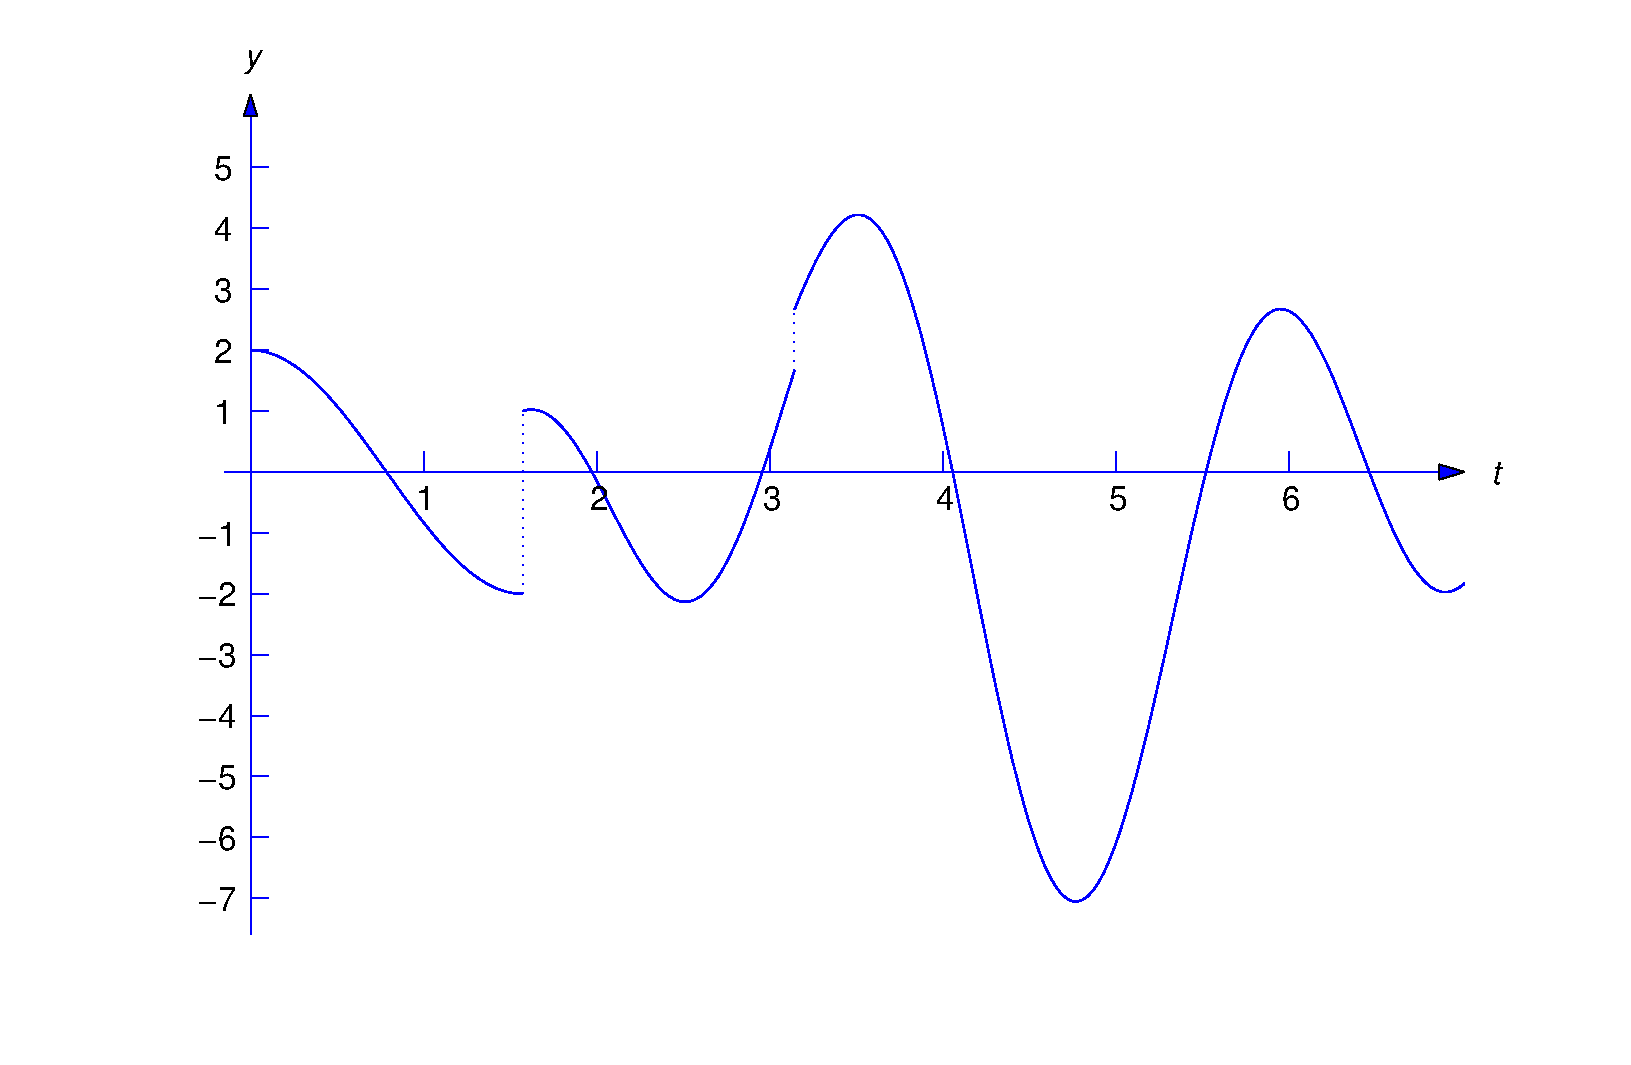
\includegraphics[bb=-78 148 689 643, width=5.67in, height=3.66in, keepaspectratio]{fig080405}
  \caption{The piecewise continuous function \eqref{eq:8.4.13}}
  \label{figure:8.4.5}
\end{figure}
\end{examplesolution}

\section*{Section 8.5}
\setcounter{chapter}{8}
\setcounter{section}{5}

\setcounter{example}{0}
\setcounter{equation}{2}
\begin{example}
  \label{example:8.5.1}\rm Solve the initial value problem
  \begin{equation}
    \label{eq:8.5.3}y''+y=f(t), \quad y(0)=2,\;y'(0)=-1,
  \end{equation}
  where
  \[
    f(t)=\left\{
    \begin{array}{rl}
      1,  & 0\le t<\displaystyle\frac{\pi}{2}, \\[2\jot]
      -1, & t\ge\displaystyle{\frac{\pi}{2}}.
    \end{array}\right.
  \]
\end{example}
\setcounter{equation}{3}
\setcounter{figure}{0}
\begin{examplesolution}
\solution The initial value problem in Step 1 is
\[
  y''+y=1,\quad y(0)=2,\quad y'(0)=-1.
\]
We leave it to you to verify that its solution is
\[
  y_{0}=1+\cos t-\sin t.
\]
Doing Step 2 yields $y_{0}(\pi/2)=0$ and $y_{0}'(\pi/2)=-1$, so the second initial value problem is
\[
  y''+y=-1,\quad y\left(\frac{\pi}{2}\right)=0,\;y'\left(\frac{\pi}{2}\right)=-1.
\]
We leave it to you to verify that the solution of this problem is
\[
  y_{1}=-1+\cos t+\sin t.
\]
Hence, the solution of \eqref{eq:8.5.3} is
\begin{equation}
  \label{eq:8.5.4}y=\left\{
  \begin{array}{rl}
    1+\cos t-\sin t,  & 0\le t<\displaystyle{\frac{\pi}{2}}, \\[2\jot]
    -1+\cos t+\sin t, & t\ge\displaystyle{\frac{\pi}{2}}
  \end{array}\right.
\end{equation}
(Figure~\ref{figure:8.5.1}).

\begin{figure}[H]
  \centering
  \relax
  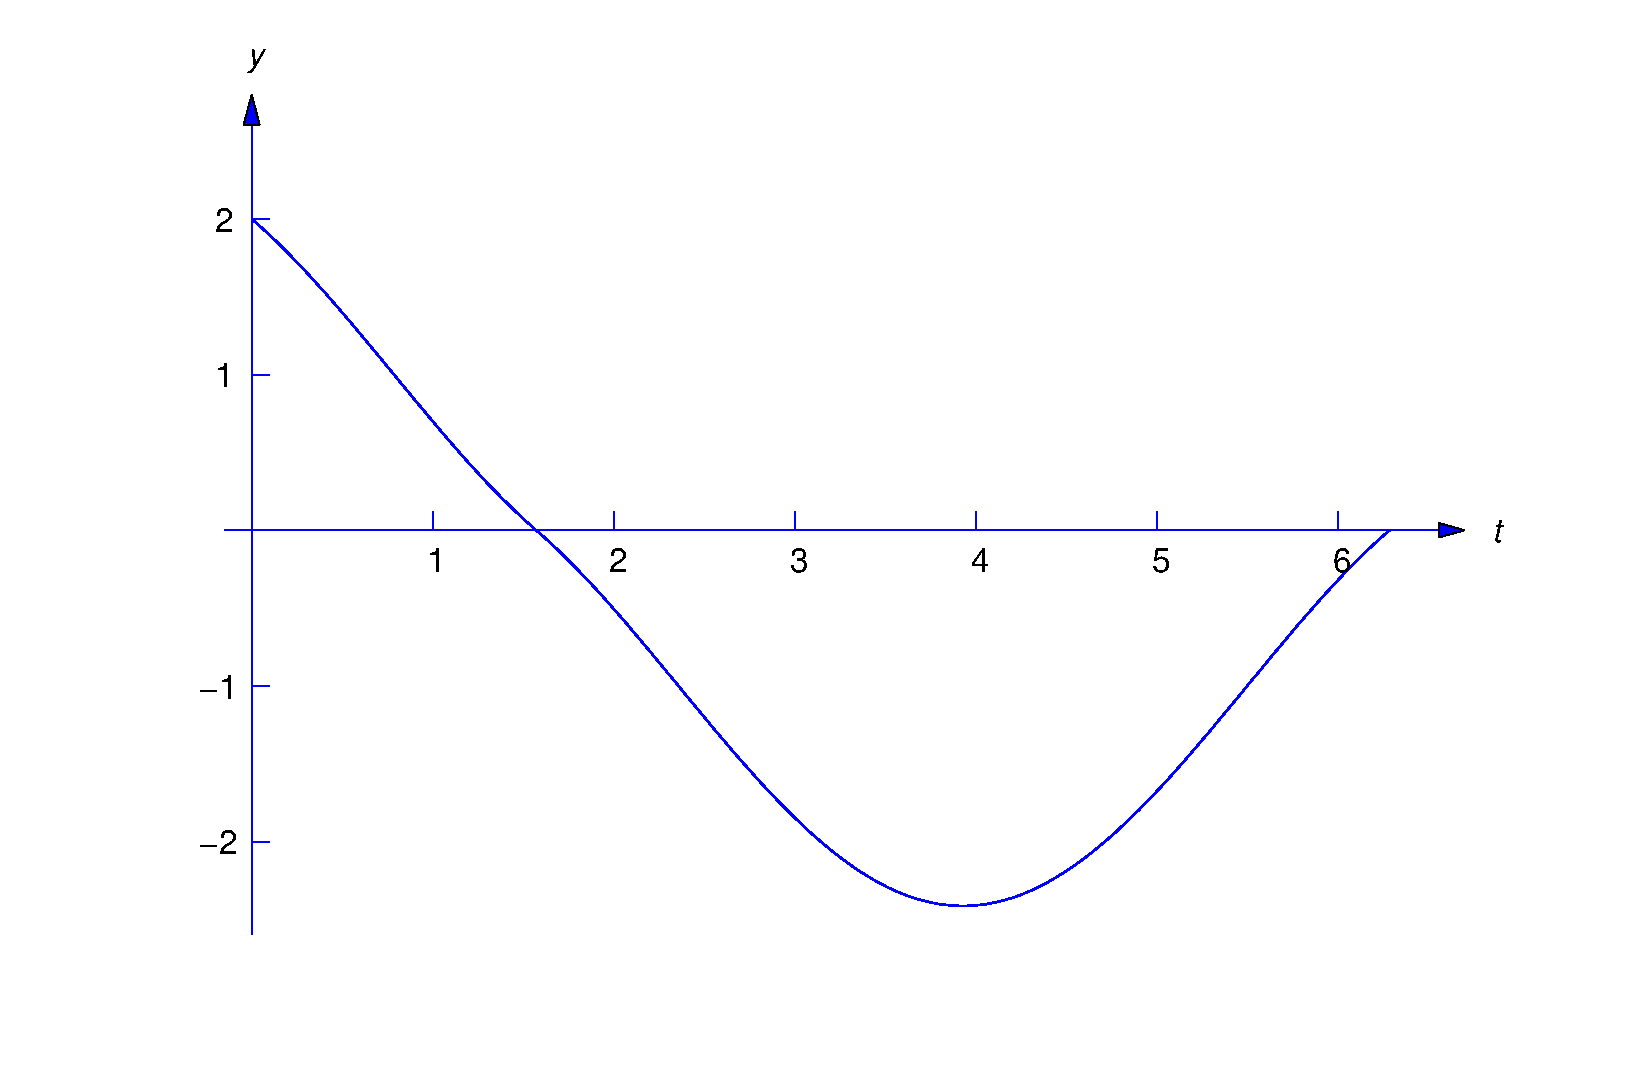
\includegraphics[bb=-78 148 689 643, width=5.67in, height=3.66in, keepaspectratio]{fig080501}
  \caption{Graph of \eqref{eq:8.5.4}}
  \label{figure:8.5.1}
\end{figure}
\end{examplesolution}

\setcounter{example}{1}
\setcounter{equation}{4}
\begin{example}
  \label{example:8.5.2}\rm \space Use the Laplace transform to solve the initial value problem
  \begin{equation}
    \label{eq:8.5.5}y''+y=f(t),\quad y(0)=2,\;y'(0)=-1,
  \end{equation}
  where
  \[
    f(t)=\left\{
    \begin{array}{cl}
      \phantom{-}1, & 0\le t<\dst{\frac{\pi}{2}}, \\
      -1,           & t\ge\dst{\frac{\pi}{2}}.
    \end{array}\right.
  \]
\end{example}
\setcounter{equation}{5}
\begin{examplesolution}
\solution Here
\[
  f(t)=1-2u\left(t-\frac{\pi}{2}\right),
\]
so Theorem~8.4.1 (with $g(t)=1$) implies that
\[
  {\cal L}(f)=\frac{1-2e^{-{\pi s/2}}}{s}.
\]
Therefore, transforming \eqref{eq:8.5.5} yields
\[
  (s^{2}+1)Y(s)=\frac{1-2e^{-{\pi s/2}}}{s}-1+2s,
\]
so
\begin{equation}
  \label{eq:8.5.6}Y(s)=(1-2e^{-{\pi s/2}})G(s)+\frac{2s-1}{s^{2}+1},
\end{equation}
with
\[
  G(s)=\frac{1}{s(s^{2}+1)}.
\]
The form for the partial fraction expansion of $G$ is
\begin{equation}
  \label{eq:8.5.7}\frac{1}{s(s^{2}+1)}=\frac{A}{s}+\frac{Bs+C}{s^{2}+1}.
\end{equation}
Multiplying through by $s(s^{2}+1)$ yields
\[
  A(s^{2}+1)+(Bs+C)s=1,
\]
or
\[
  (A+B)s^{2}+Cs+A=1.
\]
Equating coefficients of like powers of $s$ on the two sides of this equation shows that $A=1$,
$B=-A=-1$ and $C=0$. Hence, from \eqref{eq:8.5.7},
\[
  G(s)=\frac{1}{s}-\frac{s}{s^{2}+1}.
\]
Therefore
\[
  g(t)=1-\cos t.
\]
From this, \eqref{eq:8.5.6}, and Theorem~8.4.2,
\[
  y=1-\cos t-2u\left(t-\frac{\pi}{2}\right)\left(1-\cos\left(t-\frac{\pi}{2}\right)\right)+2\cos t-\sin t.
\]
Simplifying this (recalling that $\cos(t-\pi/2)=\sin t$) yields
\[
  y=1+\cos t-\sin t-2u\left(t-\frac{\pi}{2}\right)(1-\sin t),
\]
or
\[
  y=\left\{
  \begin{array}{cl}
    \phantom{-}1+\cos t-\sin t, & 0\le t<\dst{\frac{\pi}{2}}, \\
    -1+\cos t+\sin t,           & t\ge\dst{\frac{\pi}{2}},
  \end{array}\right.
\]
which is the result obtained in Example~\ref{example:8.5.1}.
\end{examplesolution}

\setcounter{example}{2}
\setcounter{equation}{7}
\begin{example}
  \label{example:8.5.3}\rm \space Solve the initial value problem
  \begin{equation}
    \label{eq:8.5.8}y''-y=f(t),\quad y(0)=-1,\;y'(0)=2,
  \end{equation}
  where
  \[
    f(t)=\left\{
    \begin{array}{cl}
      t, & 0\le t<1, \\
      1, & t\ge1.
    \end{array}\right.
  \]
\end{example}
\setcounter{equation}{8}
\begin{examplesolution}
\solution Here
\[
  f(t)=t-u(t-1)(t-1),
\]
so
\begin{eqnarray*}
  {\cal L}(f) & = & {\cal L}(t)-{\cal L}\left(u(t-1)(t-1)\right)                            \\[1\jot]
              & = & {\cal L}(t)-e^{-s}{\cal L}(t)\mbox{ (from Theorem~8.4.1)} \\[1\jot]
              & = & \frac{1}{s^{2}}-\frac{e^{-s}}{s^{2}}.
\end{eqnarray*}
Since transforming \eqref{eq:8.5.8} yields
\[
  (s^{2}-1)Y(s)={\cal L}(f)+2-s,
\]
we see that
\begin{equation}
  \label{eq:8.5.9}Y(s)=(1-e^{-s})H(s)+\frac{2-s}{s^{2}-1},
\end{equation}
where
\[
  H(s)=\frac{1}{s^{2}(s^{2}-1)}=\frac{1}{s^{2}-1}-\frac{1}{s^{2}};
\]
therefore
\begin{equation}
  \label{eq:8.5.10}h(t)=\sinh t-t.
\end{equation}
Since
\[
  {\cal L}^{-1}\left(\frac{2-s}{s^{2}-1}\right)=2\sinh t-\cosh t,
\]
we conclude from \eqref{eq:8.5.9}, \eqref{eq:8.5.10}, and Theorem~8.4.1 that
\[
  y=\sinh t-t-u(t-1)\left(\sinh(t-1)-t+1\right)+2\sinh t- \cosh t,
\]
or
\begin{equation}
  \label{eq:8.5.11}y=3\sinh t-\cosh t-t-u(t-1)\left(\sinh(t-1)-t+1\right)
\end{equation}
We leave it to you to verify that $y$ and $y'$ are continuous and $y''$ has limits from the right
and left at $t_{1}=1$.
\end{examplesolution}

\setcounter{example}{3}
\setcounter{equation}{11}
\begin{example}
  \label{example:8.5.4}\rm Solve the initial value problem
  \begin{equation}
    \label{eq:8.5.12}y''+y=f(t),\quad y(0)=0,\;y'(0)=0,
  \end{equation}
  where
  \[
    f(t)=\left\{
    \begin{array}{cl}
      0,      & 0\le t<\dst{\frac{\pi}{4}},   \\[2\jot]
      \cos2t, & \dst{\frac{\pi}{4}}\le t<\pi, \\[2\jot]
      0,      & t\ge\pi.
    \end{array}\right.
  \]
\end{example}
\setcounter{equation}{12}
\setcounter{figure}{1}
\begin{examplesolution}
\solution Here
\[
  f(t)=u(t-\pi/4)\cos2t-u(t-\pi)\cos2t,
\]
so
\begin{eqnarray*}
  {\cal L}(f) & = & {\cal L}\left(u(t-\pi/4)\cos2t\right)-{\cal L}\left(u(t-\pi)\cos2t\right)                     \\[1\jot]
              & = & e^{-{\pi s/4}}{\cal L}\left(\cos2(t+\pi/4)\right)-e^{-\pi s}{\cal L}\left(\cos2(t+\pi)\right) \\[1\jot]
              & = & -e^{-{\pi s/4}}{\cal L}(\sin2t)-e^{-\pi s}{\cal L}(\cos2t)                                    \\[1\jot]
              & = & -\frac{2e^{-{\pi s/4}}}{s^{2}+4}-\frac{se^{-\pi s}}{s^{2}+4}.
\end{eqnarray*}
Since transforming \eqref{eq:8.5.12} yields
\[
  (s^{2}+1)Y(s)={\cal L}(f),
\]
we see that
\begin{equation}
  \label{eq:8.5.13}Y(s)=e^{-{\pi s/4}}H_{1}(s)+e^{-\pi s}H_{2}(s),
\end{equation}
where
\begin{equation}
  \label{eq:8.5.14}H_{1}(s)=-\frac{2}{(s^{2}+1)(s^{2}+4)}\quad\mbox{ and }\quad H_{2}(s)=-\frac{s}{(s^{2}+1)(s^{2}+4)}.
\end{equation}
To simplify the required partial fraction expansions, we first write
\[
  \frac{1}{(x+1)(x+4)}=\frac{1}{3}\left[\frac{1}{x+1}-\frac{1}{x+4}\right].
\]
Setting $x=s^{2}$ and substituting the result in \eqref{eq:8.5.14} yields
\[
  H_{1}(s)=-\frac{2}{3}\left[\frac{1}{s^{2}+1}-\frac{1}{s^{2}+4}\right] \quad\mbox{ and }\quad H_{2}(s)=-\frac{1}{3}\left[\frac{s}{s^{2}+1}-\frac{s}{s^{2}+4}\right].
\]
The inverse transforms are
\[
  h_{1}(t)=-\frac{2}{3}\sin t+\frac{1}{3}\sin2t \quad\mbox{ and }\; h_{2}(t)=-\frac{1}{3}\cos t+\frac{1}{3}\cos2t.
\]
From \eqref{eq:8.5.13} and Theorem~8.4.2,
\begin{equation}
  \label{eq:8.5.15}y=u\left(t-\frac{\pi}{4}\right)h_{1}\left(t-\frac{\pi}{4}\right)+ u(t-\pi)h_{2}(t-\pi).
\end{equation}
Since
\begin{eqnarray*}
  h_{1}\left(t-\frac{\pi}{4}\right) & = & -\frac{2}{3}\sin\left(t-\frac{\pi}{4}\right)+\frac{1}{3}\sin2\left(t-\frac{\pi}{4}\right) \\
                                    & = & -\frac{\sqrt{2}}{3}(\sin t-\cos t)-\frac{1}{3}\cos2t
\end{eqnarray*}
and
\begin{eqnarray*}
  h_{2}(t-\pi) & = & -\frac{1}{3}\cos(t-\pi)+\frac{1}{3}\cos2(t-\pi) \\
               & = & \frac{1}{3}\cos t+\frac{1}{3}\cos2t,
\end{eqnarray*}
\eqref{eq:8.5.15} can be rewritten as
\[
  y=-\frac{1}{3}u\left(t-\frac{\pi}{4}\right)\left(\sqrt{2}(\sin t-\cos t)+\cos2t\right) +\frac{1}{3}u(t-\pi)(\cos t+\cos2t)
\]
or
\begin{equation}
  \label{eq:8.5.16}y=\left\{
  \begin{array}{cl}
    0,                                                                 & 0\le t<\dst{\frac{\pi}{4}}, \\[2\jot]
    -\dst{\frac{\sqrt{2}}{3}}(\sin t-\cos t)-\dst{\frac{1}{3}}\cos2t,  & \dst\frac{\pi}{4}\le t<\pi, \\[2\jot]
    -\dst{\frac{\sqrt{2}}{3}}\sin t+ \dst{\frac{1+\sqrt{2}}{3}}\cos t, & t\ge\pi.
  \end{array}\right.
\end{equation}
We leave it to you to verify that $y$ and $y'$ are continuous and $y''$ has limits from the right
and left at $t_{1}=\pi/4$ and $t_{2}=\pi$ (Figure~\ref{figure:8.5.2}).

\begin{figure}[H]
  \centering
  \relax
  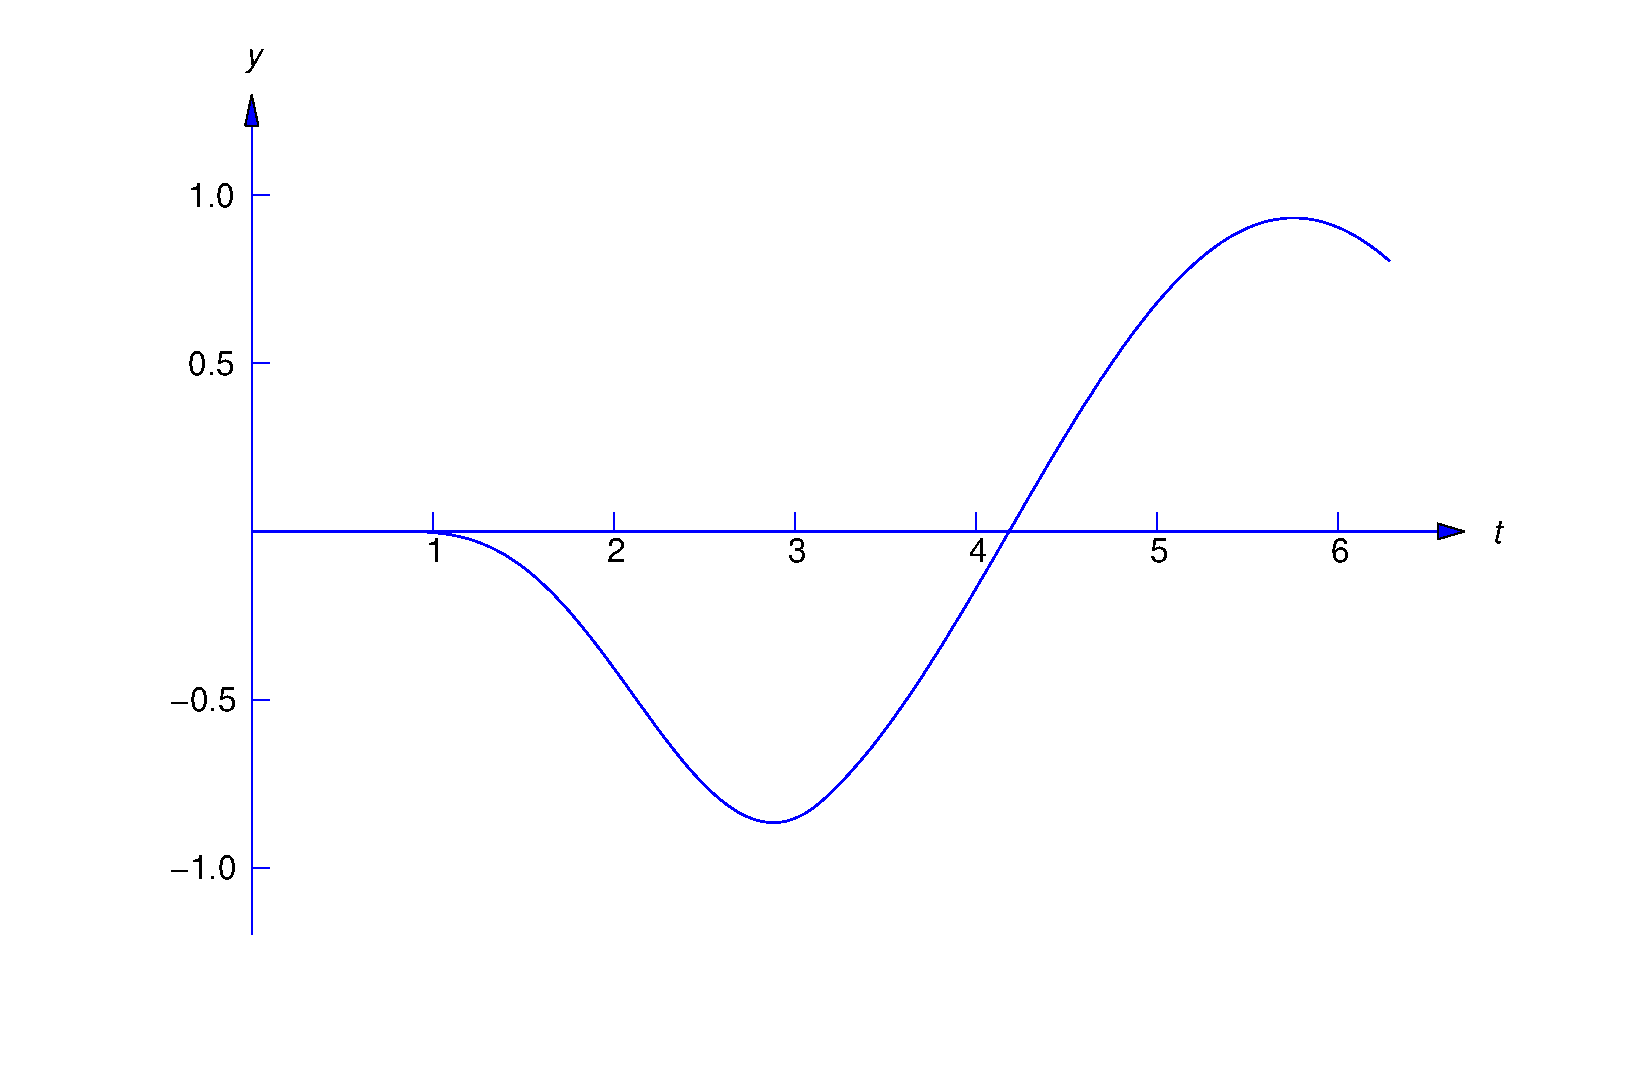
\includegraphics[bb=-78 148 689 643, width=5.67in, height=3.66in, keepaspectratio]{fig080502}
  \caption{Graph of \eqref{eq:8.5.16}}
  \label{figure:8.5.2}
\end{figure}
\end{examplesolution}

\section*{Section 8.6}
\setcounter{chapter}{8}
\setcounter{section}{6}

\setcounter{example}{0}
\begin{example}
  \label{example:8.6.1}\rm Let
  \[
    f(t)=e^{at}\mbox{\quad and \quad}g(t)=e^{bt}\qquad(a\ne b).
  \]
  Verify that ${\cal L}(f\ast g)={\cal L}(f){\cal L}(g)$, as implied by the convolution theorem.
\end{example}
\begin{examplesolution}
\solution We first compute
\[
  \begin{array}{ccccc}
    (f\ast g)(t) & = & \dst\int_{0}^{t}e^{a\tau}e^{b(t-\tau)}\,d\tau         & = & \dst e^{bt}\int_{0}^{t}e^{(a-b)\tau}d\tau       \\[2\jot]
                 & = & \dst{e^{bt}\frac{e^{(a-b)\tau}}{a-b}\,\bigg|^{t}_{0}} & = & \dst\frac{e^{bt}\left[e^{(a-b)t}-1\right]}{a-b} \\[2\jot]
                 & = & \dst\frac{e^{at}-e^{bt}}{a-b}.
  \end{array}
\]
Since
\[
  e^{at}\leftrightarrow\frac{1}{s-a}\quad\mbox{ and }\quad e^{bt}\leftrightarrow\frac{1}{s-b},
\]
it follows that
\begin{eqnarray*}
  {\cal L}(f\ast g) & = & \frac{1}{a-b}\left[\frac{1}{s-a}-\frac{1}{s-b}\right] \\[10pt]
                    & = & \frac{1}{(s-a)(s-b)}                                  \\[2\jot]
                    & = & {\cal L}(e^{at}){\cal L}(e^{bt})={\cal L}(f){\cal L}(g).
\end{eqnarray*}
\end{examplesolution}

\setcounter{example}{1}
\setcounter{equation}{6}
\begin{example}
  \label{example:8.6.2}\rm Find a formula for the solution of the initial value problem
  \begin{equation}
    \label{eq:8.6.7}y''-2y'+y=f(t),\quad y(0)=k_{0},\quad y'(0)=k_{1}.
  \end{equation}
\end{example}
\begin{examplesolution}
\solution Taking Laplace transforms in \eqref{eq:8.6.7} yields
\[
  (s^{2}-2s+1)Y(s)=F(s)+(k_{1}+k_{0}s)-2k_{0}.
\]
Therefore
\begin{eqnarray*}
  Y(s) & = & \frac{1}{(s-1)^{2}}F(s)+\frac{k_{1}+k_{0}s-2k_{0}}{(s-1)^{2}} \\[2\jot]
       & = & \frac{1}{(s-1)^{2}}F(s)+\frac{k_{0}}{s-1}+\frac{k_{1}-k_{0}}{(s-1)^{2}}.
\end{eqnarray*}
From the table of Laplace transforms,
\[
  {\cal L}^{-1}\left(\frac{k_{0}}{s-1}+\frac{k_{1}-k_{0}}{(s-1)^{2}}\right) =e^{t}\left(k_{0}+(k_{1}-k_{0})t\right).
\]
Since
\[
  \frac{1}{(s-1)^{2}}\leftrightarrow te^{t}\mbox{\quad and \quad }F(s) \leftrightarrow f(t),
\]
the convolution theorem implies that
\[
  {\cal L}^{-1}\left(\frac{1}{(s-1)^{2}}F(s)\right)= \int_{0}^{t}\tau e^{\tau}f(t-\tau)\,d\tau.
\]
Therefore the solution of \eqref{eq:8.6.7} is
\[
  y(t)=e^{t}\left(k_{0}+(k_{1}-k_{0})t\right)+\int_{0}^{t}\tau e^{\tau}f(t-\tau)\, d\tau.
\]
\end{examplesolution}

\setcounter{example}{2}
\setcounter{equation}{7}
\begin{example}
  \label{example:8.6.3}\rm Find a formula for the solution of the initial value problem
  \begin{equation}
    \label{eq:8.6.8}y''+4y=f(t),\quad y(0)=k_{0},\quad y'(0)=k_{1}.
  \end{equation}
\end{example}
\begin{examplesolution}
\solution Taking Laplace transforms in \eqref{eq:8.6.8} yields
\[
  (s^{2}+4)Y(s)=F(s)+k_{1}+k_{0}s.
\]
Therefore
\[
  Y(s)=\frac{1}{(s^{2}+4)}F(s)+\frac{k_{1}+k_{0}s}{s^{2}+4}.
\]
From the table of Laplace transforms,
\[
  {\cal L}^{-1}\left(\frac{k_{1}+k_{0}s}{s^{2}+4}\right)=k_{0}\cos2t+\frac{k_{1}}{2}\sin2t.
\]
Since
\[
  \frac{1}{(s^{2}+4)}\leftrightarrow\frac{1}{2}\sin2t\mbox{\quad and \quad}F(s)\leftrightarrow f(t),
\]
the convolution theorem implies that
\[
  {\cal L}^{-1}\left(\frac{1}{(s^{2}+4)}F(s)\right)= \frac{1}{2}\int_{0}^{t}f(t-\tau)\sin2\tau\, d\tau.
\]
Therefore the solution of \eqref{eq:8.6.8} is
\[
  y(t)=k_{0}\cos2t+\frac{k_{1}}{2}\sin2t+\frac{1}{2}\int_{0}^{t}f(t-\tau)\sin 2\tau\,d\tau.
\]
\end{examplesolution}

\setcounter{example}{3}
\setcounter{equation}{8}
\begin{example}
  \label{example:8.6.4}\rm Find a formula for the solution of the initial value problem
  \begin{equation}
    \label{eq:8.6.9}y''+2y'+2y=f(t),\quad y(0)=k_{0},\quad y'(0)=k_{1}.
  \end{equation}
\end{example}
\setcounter{equation}{9}
\begin{examplesolution}
\solution Taking Laplace transforms in \eqref{eq:8.6.9} yields
\[
  (s^{2}+2s+2)Y(s)=F(s)+k_{1}+k_{0}s+2k_{0}.
\]
Therefore
\begin{eqnarray*}
  Y(s) & = & \frac{1}{(s+1)^{2}+1}F(s)+\frac{k_{1}+k_{0}s+2k_{0}}{(s+1)^{2}+1} \\[2\jot]
       & = & \frac{1}{(s+1)^{2}+1}F(s)+\frac{(k_{1}+k_{0})+k_{0}(s+1)}{(s+1)^{2}+1}.
\end{eqnarray*}
From the table of Laplace transforms,
\[
  {\cal L}^{-1}\left(\frac{(k_{1}+k_{0})+k_{0}(s+1)}{(s+1)^{2}+1}\right)= e^{-t}\left((k_{1}+k_{0})\sin t+k_{0}\cos t\right).
\]
Since
\[
  \frac{1}{(s+1)^{2}+1}\leftrightarrow e^{-t}\sin t\mbox{\quad and \quad}F(s)\leftrightarrow f(t),
\]
the convolution theorem implies that
\[
  {\cal L}^{-1}\left(\frac{1}{(s+1)^{2}+1}F(s)\right)= \int_{0}^{t}f(t-\tau)e^{-\tau}\sin\tau \,d\tau.
\]
Therefore the solution of \eqref{eq:8.6.9} is
\begin{equation}
  \label{eq:8.6.10}y(t)=e^{-t}\left((k_{1}+k_{0})\sin t+k_{0}\cos t\right)+\int_{0}^{t}f(t-\tau)e^{-\tau}\sin\tau\,d\tau.
\end{equation}
\end{examplesolution}

\setcounter{example}{4}
\begin{example}
  \label{example:8.6.5}\rm Evaluate the convolution integral
  \[
    h(t)=\int_{0}^{t}(t-\tau)^{5}\tau^{7}d\tau.
  \]
\end{example}
\begin{examplesolution}
\solution We could evaluate this integral by expanding $(t-\tau)^{5}$ in powers of $\tau$ and then
integrating. However, the convolution theorem provides an easier way. The integral is the
convolution of $f(t)=t^{5}$ and $g(t)=t^{7}$. Since
\[
  t^{5}\leftrightarrow\frac{5!}{s^{6}}\quad\mbox{ and }\quad t^{7}\leftrightarrow\frac{7!}{s^{8}},
\]
the convolution theorem implies that
\[
  h(t)\leftrightarrow\frac{5!7!}{s^{14}}=\frac{5!7!}{13!}\,\frac{13!}{s^{14}},
\]
where we have written the second equality because
\[
  \frac{13!}{s^{14}}\leftrightarrow t^{13}.
\]
Hence,
\[
  h(t)=\frac{5!7!}{13!}\,t^{13}.
\]
\end{examplesolution}

\setcounter{example}{5}
\begin{example}
  \label{example:8.6.6}\rm Use the convolution theorem and a partial fraction expansion to evaluate
  the convolution integral
  \[
    h(t)=\int_{0}^{t}\sin a(t-\tau)\cos b\tau\,d\tau\quad(|a|\ne|b|).
  \]
\end{example}
\begin{examplesolution}
\solution Since
\[
  \sin at\leftrightarrow\frac{a}{s^{2}+a^{2}}\quad\mbox{and}\quad \cos bt\leftrightarrow\frac{s}{s^{2}+b^{2}},
\]
the convolution theorem implies that
\[
  H(s)=\frac{a}{s^{2}+a^{2}}\frac{s}{s^{2}+b^{2}}.
\]
Expanding this in a partial fraction expansion yields
\[
  H(s)=\frac{a}{b^{2}-a^{2}}\left[\frac{s}{s^{2}+a^{2}}-\frac{s}{s^{2}+b^{2}}\right].
\]
Therefore
\[
  h(t)=\frac{a}{b^{2}-a^{2}}\left(\cos at-\cos bt\right).
\]
\end{examplesolution}

\setcounter{example}{6}
\setcounter{equation}{11}
\begin{example}
  \label{example:8.6.7}\rm Solve the integral equation
  \begin{equation}
    \label{eq:8.6.12}y(t)=1+2\int_{0}^{t}e^{-2(t-\tau)}y(\tau)\,d\tau.
  \end{equation}
\end{example}
\begin{examplesolution}
\solution Taking Laplace transforms in \eqref{eq:8.6.12} yields
\[
  Y(s)=\frac{1}{s}+\frac{2}{s+2}Y(s),
\]
and solving this for $Y(s)$ yields
\[
  Y(s)=\frac{1}{s}+\frac{2}{s^{2}}.
\]
Hence,
\[
  y(t)=1+2t.
\]
\end{examplesolution}

\section*{Section 8.7}
\setcounter{chapter}{8}
\setcounter{section}{7}

\setcounter{example}{0}
\setcounter{equation}{14}
\begin{example}
  \label{example:8.7.1} \rm Find the solution of the initial value problem
  \begin{equation}
    \label{eq:8.7.15}y''-2y'+y=\delta(t-t_{0}),\quad y(0)=0,\quad y'(0)=0,
  \end{equation}
  where $t_{0}>0$. Then interpret the solution for the case where $t_{0}=0$.
\end{example}
\setcounter{figure}{2}
\begin{examplesolution}
\solution Here
\[
  w={\cal L}^{-1}\left(\frac{1}{s^{2}-2s+1}\right)={\cal L}^{-1}\left(\frac{1}{(s-1)^{2}}\right)=te^{t},
\]
so Definition~8.7.2 yields
\[
  y=u(t-t_{0})(t-t_{0})e^{t-t_{0}}
\]
as the solution of \eqref{eq:8.7.15} if $t_{0}>0$. If $t_{0}=0$, then \eqref{eq:8.7.15} doesn't have
a solution; however, $y=u(t)te^{t}$ (which we would usually write simply as $y=te^{t}$) is the
solution of the modified initial value problem
\[
  y''-2y'+y=\delta(t),\quad y(0)=0,\quad y_{-}'(0)=0.
\]

The graph of $y=u(t-t_{0})(t-t_{0})e^{t-t_{0}}$ is shown in Figure~\ref{figure:8.7.3} \bbox

\begin{figure}[H]
  \centering
  \relax
  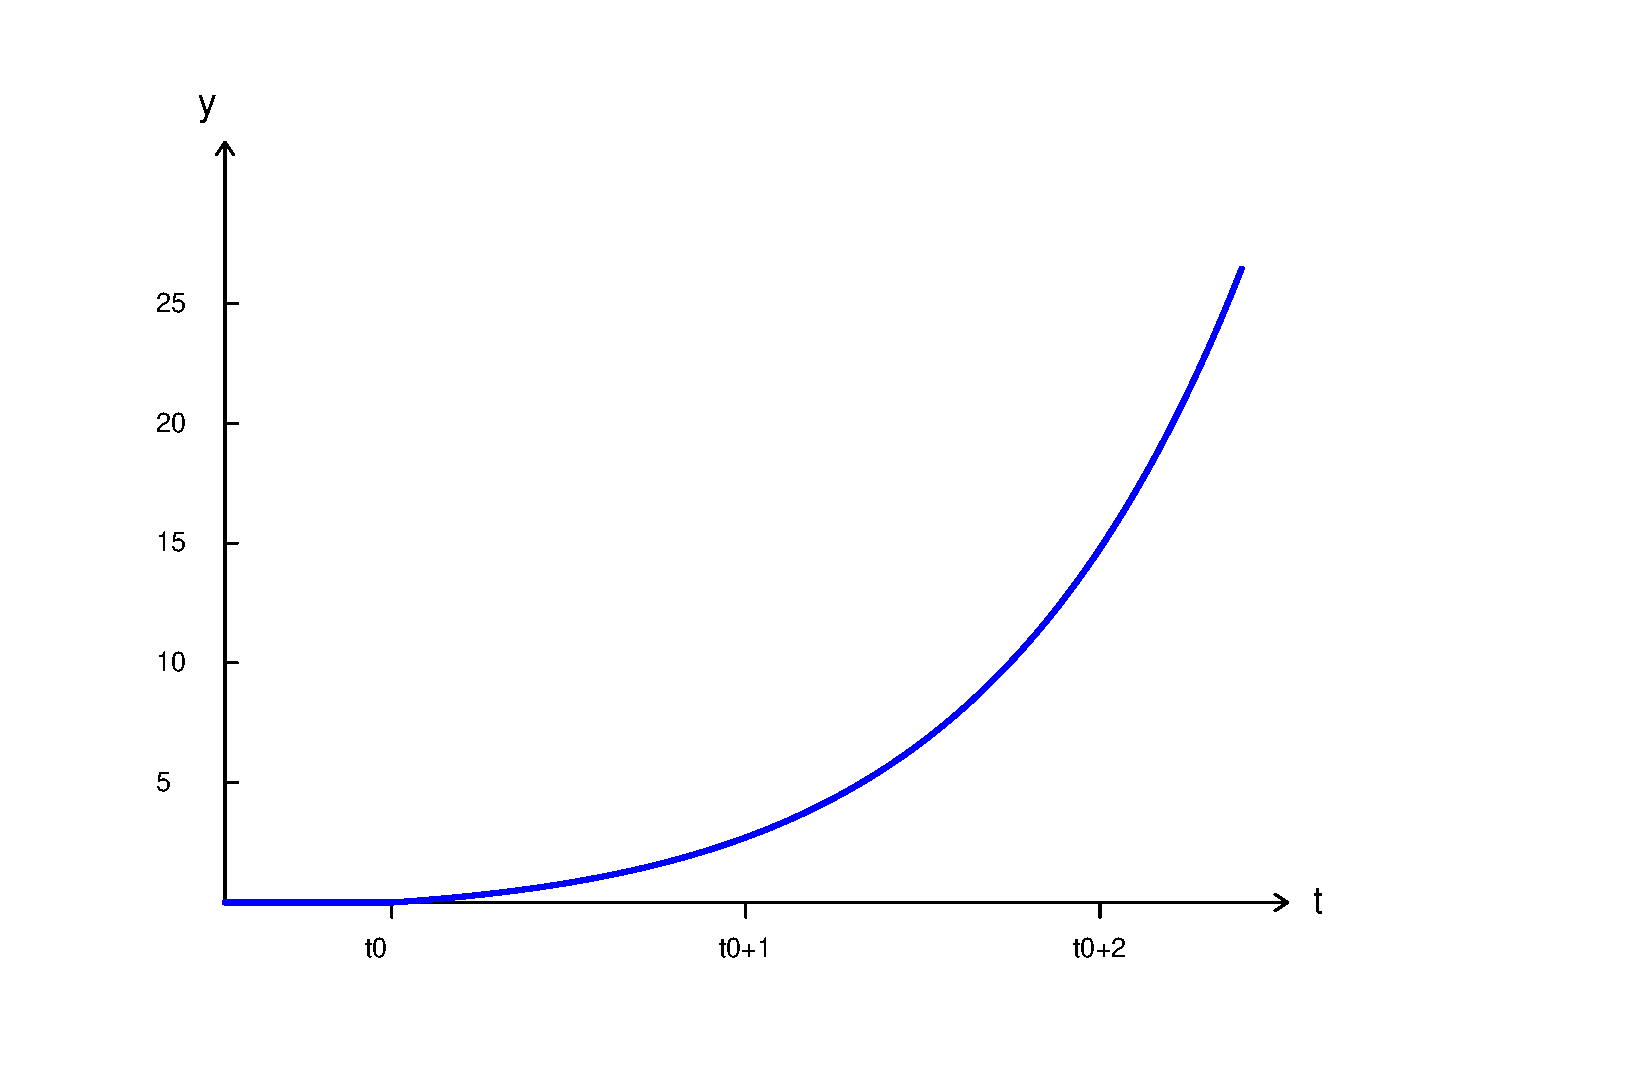
\includegraphics[ width=5.67in, height=3.66in, keepaspectratio]{fig080703}
  \caption{$y=u(t-t_{0})(t-t_{0})e^{t-t_{0}}$}
  \label{figure:8.7.3}
\end{figure}
\end{examplesolution}

\setcounter{example}{1}
\setcounter{equation}{15}
\begin{example}
  \label{example:8.7.2} \rm Solve the initial value problem
  \begin{equation}
    \label{eq:8.7.16}y''+6y'+5y=3e^{-2t}+2\delta(t-1),\quad y(0)=-3,\quad y'(0)=2.
  \end{equation}
\end{example}
\setcounter{equation}{16}
\setcounter{figure}{3}
\begin{examplesolution}
\solution We leave it to you to show that the solution of
\[
  y''+6y'+5y=3e^{-2t},\quad y(0)=-3,\;y'(0)=2
\]
is
\[
  \hat{y}=-e^{-2t}+\frac{1}{2}e^{-5t}-\frac{5}{2}e^{-t}.
\]
Since
\[
  \begin{array}{ccccl}
    w(t) & = & {\cal L}^{-1}\left(\dst\frac{1}{s^{2}+6s+5}\right)                     & = & {\cal L}^{-1}\left(\dst\frac{1}{(s+1)(s+5)}\right) \\[2\jot]
         & = & \dst{\frac{1}{4}{\cal L}^{-1}\left(\frac{1}{s+1}-\frac{1}{s+5}\right)} & = & \dst\frac{e^{-t}-e^{-5t}}{4},
  \end{array}
\]
the solution of \eqref{eq:8.7.16} is
\begin{equation}
  \label{eq:8.7.17}y=-e^{-2t}+\frac{1}{2}e^{-5t}-\frac{5}{2}e^{-t}+u(t-1)\frac{e^{-(t-1)}-e^{-5(t-1)}}{2}
\end{equation}
(Figure~\ref{figure:8.7.4})\bbox.

\begin{figure}[H]
  \relax
  \begin{minipage}[b]{0.5\linewidth}
    \centering
    \scalebox{.65}{
    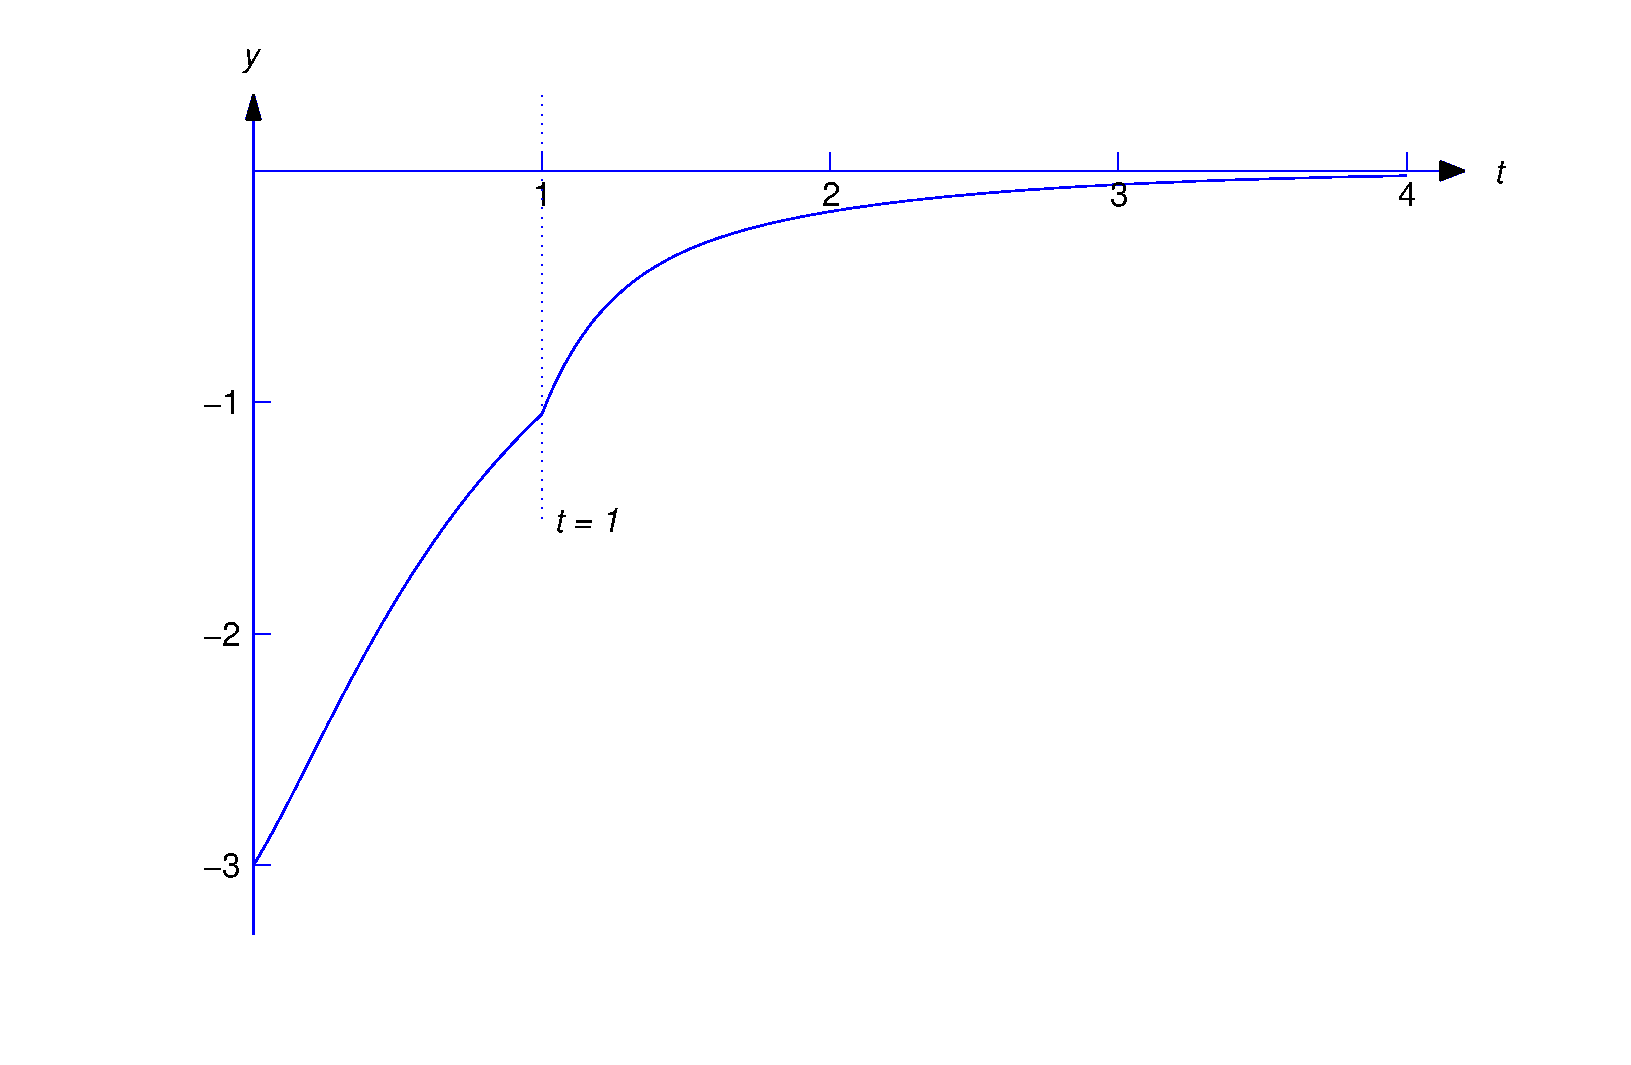
\includegraphics[bb=-78 148 689 643, width=5.67in, height=3.66in, keepaspectratio]{fig080704}}
    \caption{Graph of \eqref{eq:8.7.17}}
    \label{figure:8.7.4}
  \end{minipage}
  \begin{minipage}[b]{0.5\linewidth}
    \centering
    \scalebox{.65}{
    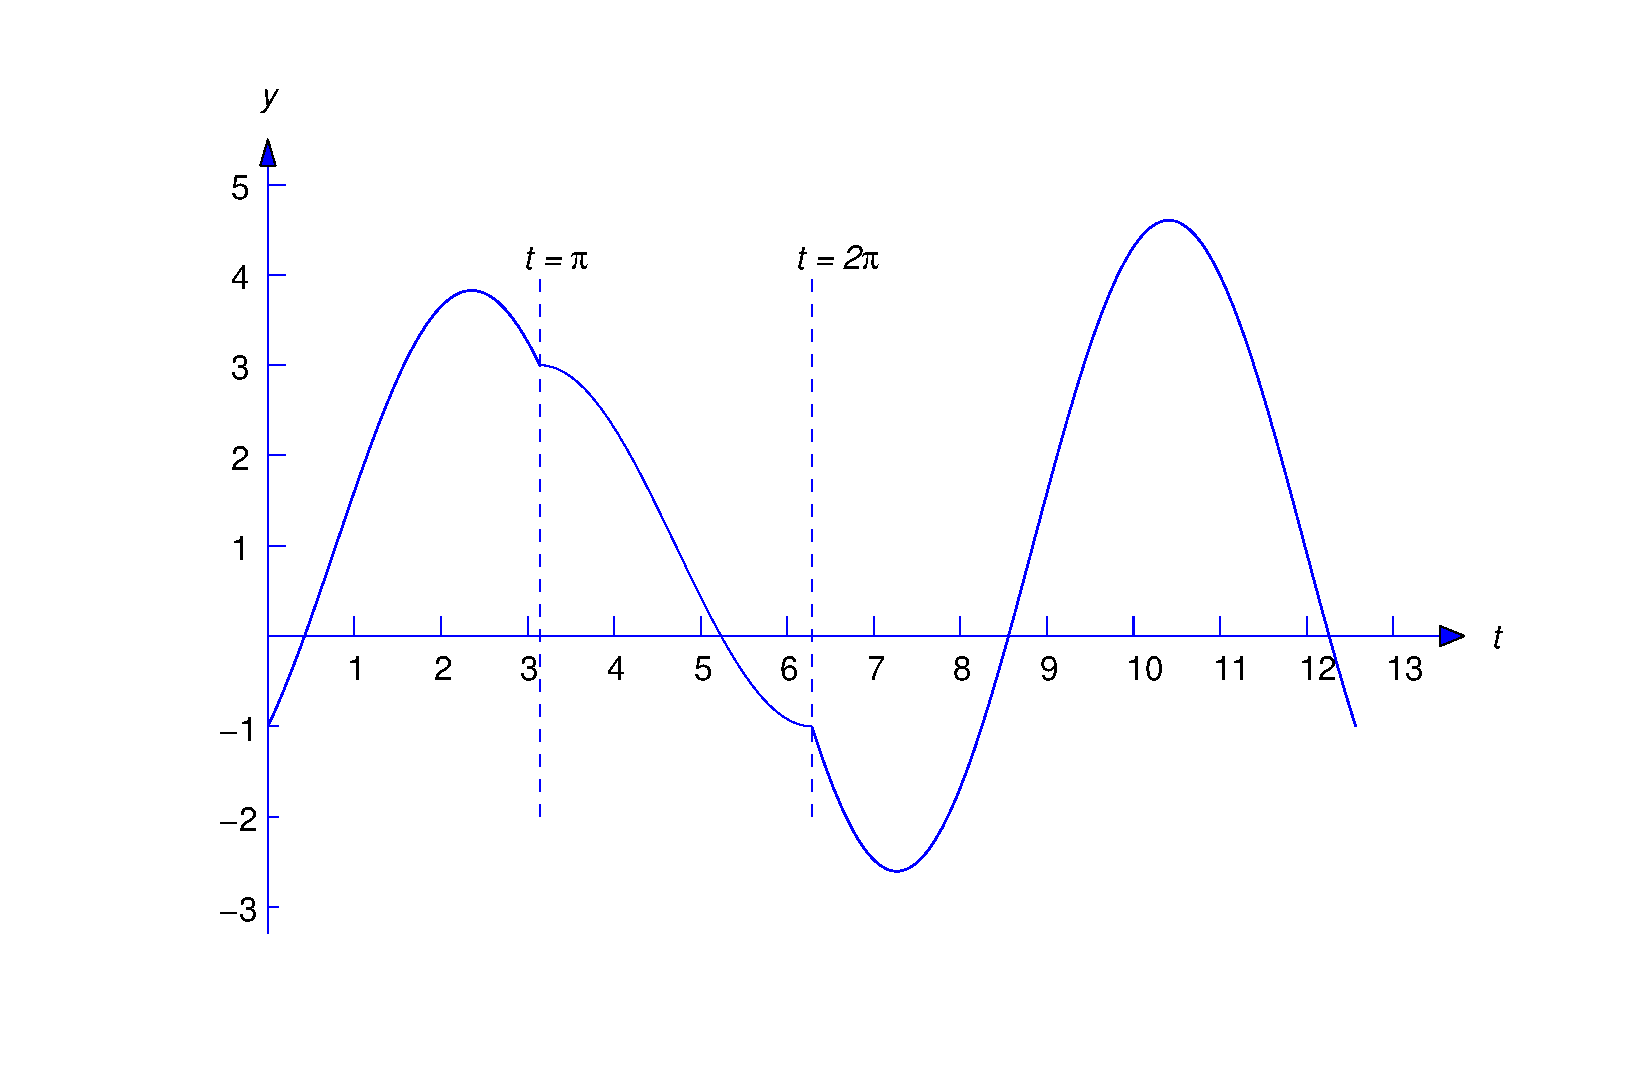
\includegraphics[bb=-78 148 689 643, width=5.67in, height=3.66in, keepaspectratio]{fig080705}}
    \caption{Graph of \eqref{eq:8.7.19}}
    \label{figure:8.7.5}
  \end{minipage}
\end{figure}
\end{examplesolution}

\setcounter{example}{2}
\setcounter{equation}{17}
\begin{example}
  \label{example:8.7.3} \rm Solve the initial value problem
  \begin{equation}
    \label{eq:8.7.18}y''+y=1+2\delta(t-\pi)-3\delta(t-2\pi),\quad y(0)=-1,\;y'(0)=2.
  \end{equation}
\end{example}
\setcounter{equation}{18}
\begin{examplesolution}
\solution We leave it to you to show that
\[
  \hat{y}=1-2\cos t+2\sin t
\]
is the solution of
\[
  y''+y=1,\quad y(0)=-1,\quad y'(0)=2.
\]
Since
\[
  w={\cal L}^{-1}\left(\frac{1}{s^{2}+1}\right)=\sin t,
\]
the solution of \eqref{eq:8.7.18} is
\begin{eqnarray*}
  y & = & 1-2\cos t+2\sin t+2u(t-\pi)\sin(t-\pi)-3u(t-2\pi)\sin(t-2\pi) \\
    & = & 1-2\cos t+2\sin t-2u(t-\pi)\sin t-3u(t-2\pi)\sin t,
\end{eqnarray*}
or
\begin{equation}
  \label{eq:8.7.19}y=\left\{
  \begin{array}{cl}
    1-2\cos t+2\sin t, & 0\le t<\pi,    \\[5pt]
    1-2\cos t,         & \pi\le t<2\pi, \\[5pt]
    1-2\cos t-3\sin t, & t\ge2\pi
  \end{array}\right.
\end{equation}
(Figure~\ref{figure:8.7.5}).
\end{examplesolution}

\section*{Section 9.1}
\phantomsection
\addcontentsline{toc}{chapter}{Chapter 9}
\setcounter{chapter}{9}
\setcounter{section}{1}

\setcounter{example}{0}
\setcounter{equation}{4}
\begin{example}
  \label{example:9.1.1}\rm The equation
  \begin{equation}
    \label{eq:9.1.5}x^{3}y'''-x^{2}y''-2xy'+6y=0
  \end{equation}
  is normal and has the solutions $y_{1}=x^{2}$, $y_{2}=x^{3}$, and $y_{3}=1/x$ on $(-\infty,0)$ and
  $(0,\infty)$. Show that $\{y_{1},y_{2},y_{3}\}$ is linearly independent on $(-\infty,0)$ and
  $(0,\infty)$. Then find the general solution of \eqref{eq:9.1.5} on $(-\infty,0)$ and
  $(0,\infty)$.
\end{example}
\setcounter{equation}{5}
\begin{examplesolution}
\solution Suppose
\begin{equation}
  \label{eq:9.1.6}c_{1}x^{2}+c_{2}x^{3}+\frac{c_{3}}{x}=0
\end{equation}
on $(0,\infty)$. We must show that $c_{1}=c_{2}=c_{3}=0$. Differentiating \eqref{eq:9.1.6} twice
yields the system
\begin{equation}
  \label{eq:9.1.7}
  \begin{array}{rcl}
    c_{1}x^{2}+c_{2}x^{3}+\dst\frac{c_{3}}{x}   & = & 0  \\[2\jot]
    2c_{1}x+3c_{2}x^{2}-\dst\frac{c_{3}}{x^{2}} & = & 0  \\[2\jot]
    2c_{1}+6c_{2}x+\dst\frac{2c_{3}}{x^{3}}     & = & 0.
  \end{array}
\end{equation}
If \eqref{eq:9.1.7} holds for all $x$ in $(0,\infty)$, then it certainly holds at $x=1$; therefore,
\begin{equation}
  \label{eq:9.1.8}
  \begin{array}{rcl}
    \phantom{2}c_{1}+\phantom{3}c_{2}+\phantom{2}c_{3} & = & 0  \\
    2c_{1}+3c_{2}-\phantom{2}c_{3}                     & = & 0  \\
    2c_{1}+6c_{2}+2c_{3}                               & = & 0.
  \end{array}
\end{equation}
By solving this system directly, you can verify that it has only the trivial solution
$c_{1}=c_{2}=c_{3}=0$; however, for our purposes it's more useful to recall from linear algebra that
a homogeneous linear system of $n$ equations in $n$ unknowns has only the trivial solution if its
determinant is nonzero. Since the determinant of \eqref{eq:9.1.8} is
\[
  \left|
  \begin{array}{rrr}
    1 & 1 & 1  \\
    2 & 3 & -1 \\
    2 & 6 & 2
  \end{array}\right|= \left|
  \begin{array}{rrr}
    1 & 0 & 0  \\
    2 & 1 & -3 \\
    2 & 4 & 0
  \end{array}\right|=12,
\]
it follows that \eqref{eq:9.1.8} has only the trivial solution, so $\{y_{1},y_{2},y_{3}\}$ is
linearly independent on $(0,\infty)$. Now Theorem~9.1.2 implies that
\[
  y=c_{1}x^{2}+c_{2}x^{3}+\frac{c_{3}}{x}
\]
is the general solution of \eqref{eq:9.1.5} on $(0,\infty)$. To see that this is also true on
$(-\infty,0)$, assume that \eqref{eq:9.1.6} holds on $(-\infty,0)$. Setting $x=-1$ in
\eqref{eq:9.1.7} yields
\begin{eqnarray*}
  \phantom{-2}c_{1}-\phantom{3}c_{2}-\phantom{2}c_{3} & = & 0 \\
  -2c_{1}+3c_{2}-\phantom{2}c_{3}                     & = & 0 \\
  \phantom{-}2c_{1}-6c_{2}-2c_{3}                     & = & 0.
\end{eqnarray*}
Since the determinant of this system is
\[
  \left|
  \begin{array}{rrr}
    1  & -1 & -1 \\
    -2 & 3  & -1 \\
    2  & -6 & -2
  \end{array}\right|= \left|
  \begin{array}{rrr}
    1  & 0  & 0  \\
    -2 & 1  & -3 \\
    2  & -4 & 0
  \end{array}\right|=-12,
\]
it follows that $c_{1}=c_{2}=c_{3}=0$; that is, $\{y_{1},y_{2},y_{3}\}$ is linearly independent on
$(-\infty,0)$.
\end{examplesolution}

\setcounter{example}{1}
\setcounter{equation}{8}
\begin{example}
  \label{example:9.1.2}\rm The equation
  \begin{equation}
    \label{eq:9.1.9}y^{(4)}+y'''-7y''-y'+6y=0
  \end{equation}
  is normal and has the solutions $y_{1}=e^{x}$, $y_{2}=e^{-x}$, $y_{3}=e^{2x}$, and $y_{4}=e^{-3x}$
  on $(-\infty,\infty)$. (Verify.) Show that $\{y_{1},y_{2},y_{3},y_{4}\}$ is linearly independent
  on $(-\infty,\infty)$. Then find the general solution of \eqref{eq:9.1.9}.
\end{example}
\setcounter{equation}{9}
\begin{examplesolution}
\solution Suppose $c_{1}$, $c_{2}$, $c_{3}$, and $c_{4}$ are constants such that
\begin{equation}
  \label{eq:9.1.10}c_{1}e^{x}+c_{2}e^{-x}+c_{3}e^{2x}+c_{4}e^{-3x}=0
\end{equation}
for all $x$. We must show that $c_{1}=c_{2}=c_{3}=c_{4}=0$. Differentiating \eqref{eq:9.1.10} three
times yields the system
\begin{equation}
  \label{eq:9.1.11}
  \begin{array}{rcl}
    c_{1}e^{x}+c_{2}e^{-x}+\phantom{2}c_{3}e^{2x}+\phantom{27}c_{4}e^{-3x} & = & 0  \\
    c_{1}e^{x}-c_{2}e^{-x}+2c_{3}e^{2x}-\phantom{2}3c_{4}e^{-3x}           & = & 0  \\
    c_{1}e^{x}+c_{2}e^{-x}+4c_{3}e^{2x}+\phantom{2}9c_{4}e^{-3x}           & = & 0  \\
    c_{1}e^{x}-c_{2}e^{-x}+8c_{3}e^{2x}-27c_{4}e^{-3x}                     & = & 0.
  \end{array}
\end{equation}
If \eqref{eq:9.1.11} holds for all $x$, then it certainly holds for $x=0$. Therefore
\[
  \begin{array}{rcl}
    c_{1}+c_{2}+\phantom{2}c_{3}+\phantom{27}c_{4} & = & 0  \\
    c_{1}-c_{2}+2c_{3}-\phantom{2}3c_{4}           & = & 0  \\
    c_{1}+c_{2}+4c_{3}+\phantom{2}9c_{4}           & = & 0  \\
    c_{1}-c_{2}+8c_{3}-27c_{4}                     & = & 0.
  \end{array}
\]
The determinant of this system is
\begin{equation}
  \label{eq:9.1.12}
  \begin{array}{rcl}
    \left|\begin{array}{rrrr}1&1&1&1\\1&-1&2&-3\\1&1&4&9\\ 1&-1&8&-27\end{array}\right| & = & \left|\begin{array}{rrrr}1&1&1&1\\0&-2&1&-4\\0&0&3&8\\ 0&-2&7&-28\end{array}\right| =\left|\begin{array}{rrr}-2&1&-4\\0&3&8\\ -2&7&-28\end{array}\right| \\[8\jot]
                                                                                        & = & \left|\begin{array}{rrr}-2&1&-4\\0&3&8 \\0&6&-24\end{array}\right|= -2\left|\begin{array}{rr}3&8\\6&-24\end{array}\right|=240,
  \end{array}
\end{equation}
so the system has only the trivial solution $c_{1}=c_{2}=c_{3}=c_{4}=0$. Now
Theorem~9.1.2 implies that
\[
  y=c_{1}e^{x}+c_{2}e^{-x}+c_{3}e^{2x}+c_{4}e^{-3x}
\]
is the general solution of \eqref{eq:9.1.9}.
\end{examplesolution}

\setcounter{example}{2}
\begin{example}
  \label{example:9.1.3} \rm In Example~\ref{example:9.1.1} we saw that the solutions $y_{1}=x^{2}$,
  $y_{2}=x^{3}$, and $y_{3}=1/x$ of
  \[
    x^{3}y'''-x^{2}y''-2xy'+6y=0
  \]
  are linearly independent on $(-\infty,0)$ and $(0,\infty)$. Calculate the Wronskian of
  $\{y_{1},y_{2},y_{3}\}$.
\end{example}
\begin{examplesolution}
\solution If $x\ne0$, then
\[
  W(x)=\left|
  \begin{array}{ccc}
    x^{2} & \phantom{2}x^{3}     & \phantom{-}\dst\frac{1}{x}     \\[2\jot]
    2x    & 3x^{2}\phantom{^{2}} & \dst-\dst\frac{1}{x^{2}}       \\[2\jot]
    2     & 6x\phantom{x^{2}}    & \phantom{-}\dst\frac{2}{x^{3}}
  \end{array}
  \right| =2x^{3}\left|
  \begin{array}{ccc}
    1 & \phantom{3}x & \phantom{-}\dst\frac{1}{x^{3}} \\[2\jot]
    2 & 3x           & -\dst\frac{1}{x^{3}}           \\[2\jot]
    1 & 3x           & \phantom{-}\dst\frac{1}{x^{3}}
  \end{array}\right|,
\]
where we factored $x^{2}$, $x$, and $2$ out of the first, second, and third rows of $W(x)$,
respectively. Adding the second row of the last determinant to the first and third rows yields
\[
  W(x)=2x^{3}\left|
  \begin{array}{ccc}
    3 & 4x & \phantom{-}0         \\[2\jot]
    2 & 3x & -\dst\frac{1}{x^{3}} \\[2\jot]
    3 & 6x & \phantom{-}0
  \end{array}\right| =2x^{3}\left(\frac{1}{x^{3}}\right)\left|
  \begin{array}{cc}
    3 & 4x \\
    3 & 6x
  \end{array}\right|=12x.
\]
Therefore $W(x)\ne0$ on $(-\infty,0)$ and $(0,\infty)$.
\end{examplesolution}

\setcounter{example}{3}
\begin{example}
  \label{example:9.1.4} \rm In Example~\ref{example:9.1.2} we saw that the solutions $y_{1}=e^{x}$,
  $y_{2}=e^{-x}$, $y_{3}=e^{2x}$, and $y_{4}=e^{-3x}$ of
  \[
    y^{(4)}+y'''-7y''-y'+6y=0
  \]
  are linearly independent on every open interval. Calculate the Wronskian of
  $\{y_{1},y_{2},y_{3},y_{4}\}$.
\end{example}
\begin{examplesolution}
\solution For all $x$,
\[
  W(x)=\left|
  \begin{array}{rrrr}
    e^{x} & e^{-x}  & e^{2x}  & e^{-3x}    \\
    e^{x} & -e^{-x} & 2e^{2x} & -3e^{-3x}  \\
    e^{x} & e^{-x}  & 4e^{2x} & 9e^{-3x}   \\
    e^{x} & -e^{-x} & 8e^{2x} & -27e^{-3x}
  \end{array}\right|.
\]
Factoring the exponential common factor from each row yields
\[
  W(x)=e^{-x}\left|
  \begin{array}{rrrr}
    1 & 1  & 1 & 1   \\
    1 & -1 & 2 & -3  \\
    1 & 1  & 4 & 9   \\
    1 & -1 & 8 & -27
  \end{array}\right|=240e^{-x},
\]
from \eqref{eq:9.1.12}.
\end{examplesolution}

\section*{Section 9.2}
\setcounter{chapter}{9}
\setcounter{section}{2}

\setcounter{example}{0}
\setcounter{equation}{2}
\begin{example}
  \label{example:9.2.1} \rm \mbox{}
  \newline
  \begin{alist}
    \item % (a)
    Find the general solution of
    \begin{equation}
      \label{eq:9.2.3}y'''-6y''+11y'-6y=0.
    \end{equation}

    \item % (b)
    Solve the initial value problem
    \begin{equation}
      \label{eq:9.2.4}y'''-6y''+11y'-6y=0,\quad y(0)=4,\quad y'(0)=5,\quad y''(0)=9.
    \end{equation}
  \end{alist}
\end{example}
\setcounter{equation}{4}
\setcounter{figure}{0}
\begin{examplesolution}
\solution The characteristic polynomial of \eqref{eq:9.2.3} is
\[
  p(r)=r^{3}-6r^{2}+11r-6=(r-1)(r-2)(r-3).
\]
Therefore $\{e^{x},e^{2x},e^{3x}\}$ is a set of solutions of \eqref{eq:9.2.3}. It is a fundamental
set, since its Wronskian is
\[
  W(x)=\left|
  \begin{array}{rrr}
    e^{x} & e^{2x}  & e^{3x}  \\
    e^{x} & 2e^{2x} & 3e^{3x} \\
    e^{x} & 4e^{2x} & 9e^{3x}
  \end{array}\right|= e^{6x}\left|
  \begin{array}{rrr}
    1 & 1 & 1 \\
    1 & 2 & 3 \\
    1 & 4 & 9
  \end{array}\right|=2e^{6x}\ne0.
\]
Therefore the general solution of \eqref{eq:9.2.3} is
\begin{equation}
  \label{eq:9.2.5}y=c_{1}e^{x}+c_{2}e^{2x}+c_{3}e^{3x}.
\end{equation}

\solutionpart{b} We must determine $c_{1}$, $c_{2}$ and $c_{3}$ in \eqref{eq:9.2.5} so that $y$
satisfies the initial conditions in \eqref{eq:9.2.4}. Differentiating \eqref{eq:9.2.5} twice yields
\begin{equation}
  \label{eq:9.2.6}
  \begin{array}{rcl}
    y'  & = & c_{1}e^{x}+2c_{2}e^{2x}+3c_{3}e^{3x}  \\
    y'' & = & c_{1}e^{x}+4c_{2}e^{2x}+9c_{3}e^{3x}.
  \end{array}
\end{equation}
Setting $x=0$ in \eqref{eq:9.2.5} and \eqref{eq:9.2.6} and imposing the initial conditions yields
\[
  \begin{array}{rcl}
    c_{1}+\phantom{2}c_{2}+\phantom{3}c_{3} & = & 4  \\
    c_{1}+2c_{2}+3c_{3}                     & = & 5  \\
    c_{1}+4c_{2}+9c_{3}                     & = & 9.
  \end{array}
\]
The solution of this system is $c_{1}=4$, $c_{2}=-1$, $c_{3}=1$. Therefore the solution of
\eqref{eq:9.2.4} is
\[
  y=4e^{x}-e^{2x}+e^{3x}
\]
(Figure~\ref{figure:9.2.1}). \bbox

\begin{figure}[H]
  \centering
  \relax
  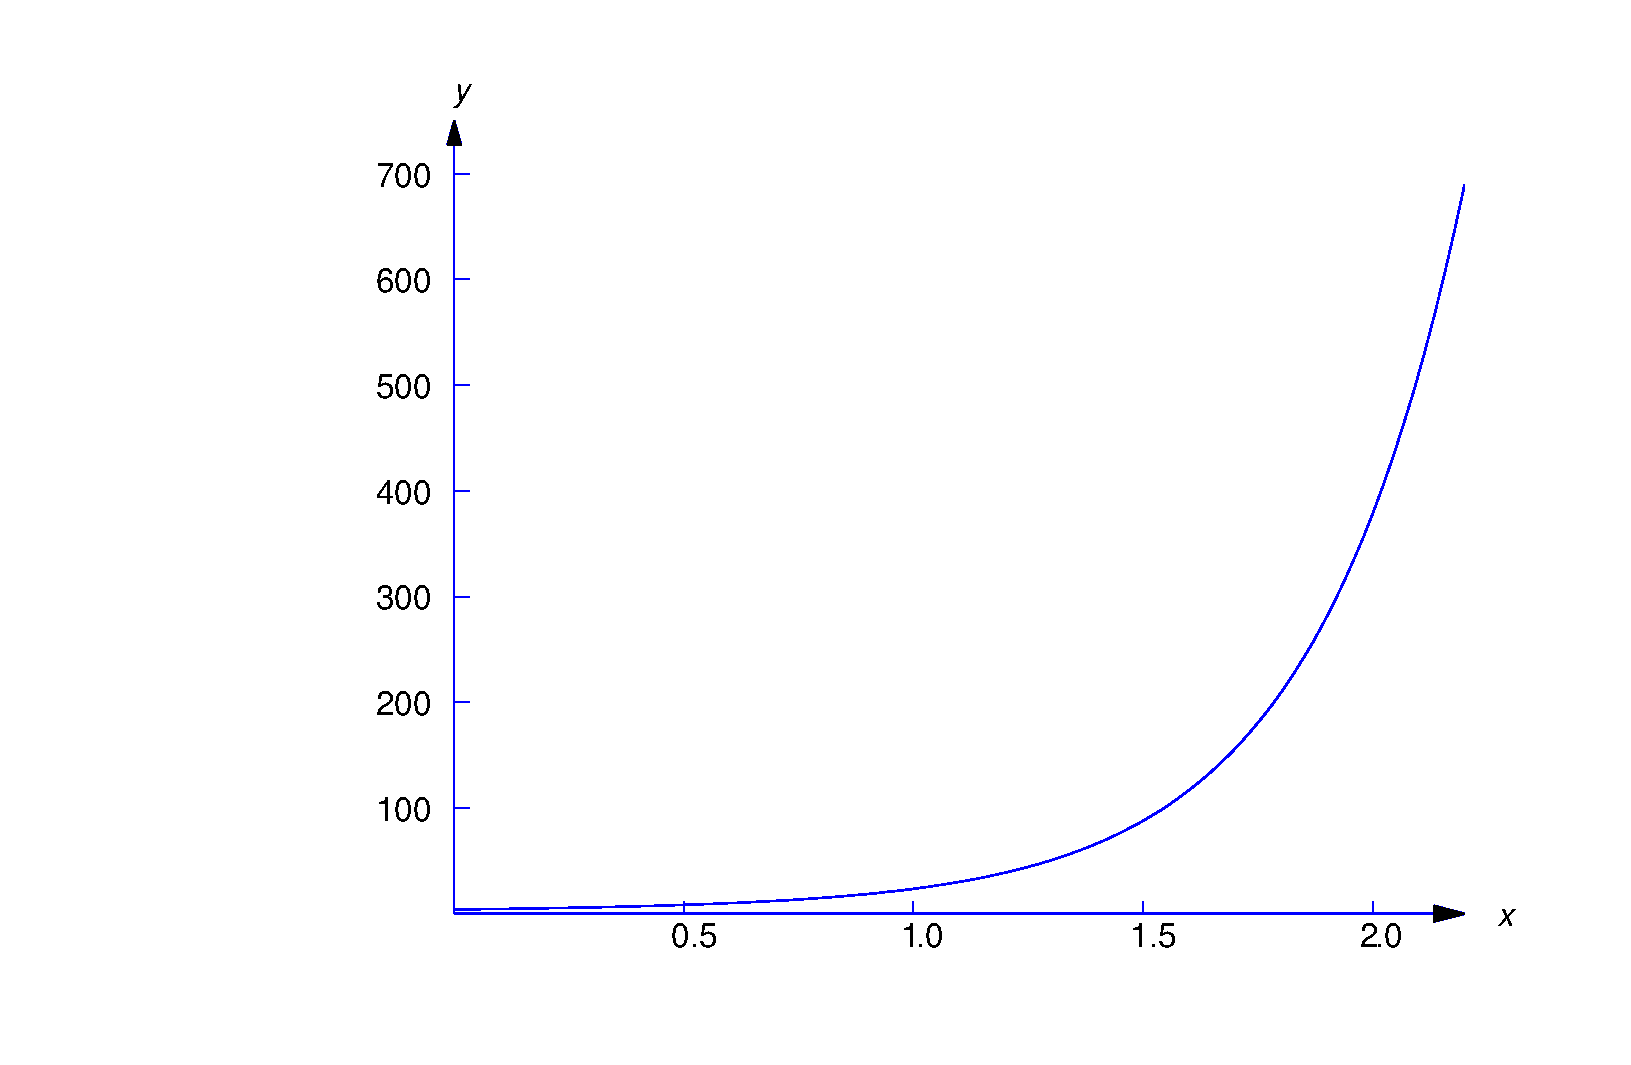
\includegraphics[bb=-78 148 689 643, width=5.67in, height=3.66in, keepaspectratio]{fig090201}
  \caption{$y=4e^{x}-e^{2x}+e^{3x}$}
  \label{figure:9.2.1}
\end{figure}
\end{examplesolution}

\setcounter{example}{1}
\setcounter{equation}{6}
\begin{example}
  \label{example:9.2.2} \rm Consider the polynomial
  \[
    p(r)=r^{3}-r^{2}+r-1
  \]
  and the associated polynomial operator
  \[
    p(D)=D^{3}-D^{2}+D-1.
  \]
  Since $p(r)$ can be factored as
  \[
    p(r)=(r-1)(r^{2}+1)=(r^{2}+1)(r-1),
  \]
  it's reasonable to expect that p(D) can be factored as
  \begin{equation}
    \label{eq:9.2.7}p(D)=(D-1)(D^{2}+1)=(D^{2}+1)(D-1).
  \end{equation}
  However, before we can make this assertion we must {\relax\it define\/} what we mean by
  saying that two operators are equal, and what we mean by the products of operators in
  \eqref{eq:9.2.7}. We say that two operators are equal if they apply to the same functions and
  always produce the same result. The definition of the products in \eqref{eq:9.2.7} is this: if
  $y$ is any three-times differentiable function then
  \begin{alist}
    \item % (a)
    $(D-1)(D^{2}+1)y$ is the function obtained by first applying $D^{2}+1$ to $y$ and then applying
    $D-1$ to the resulting function

    \item % (b)
    $(D^{2}+1)(D-1)y$ is the function obtained by first applying $D-1$ to $y$ and then applying
    $D^{2}+1$ to the resulting function.
  \end{alist}
  From \part{a},
  \begin{equation}
    \label{eq:9.2.8}
    \begin{array}{rcl}
      (D-1)(D^{2}+1)y & = & (D-1)[(D^{2}+1)y]                 \\
                      & = & (D-1)(y''+y)=D(y''+y)-(y''+y)     \\
                      & = & (y'''+y')-(y''+y)                 \\
                      & = & y'''-y''+y'-y=(D^{3}-D^{2}+D-1)y.
    \end{array}
  \end{equation}
  This implies that
  \[
    (D-1)(D^{2}+1)=(D^{3}-D^{2}+D-1).
  \]
  From \part{b},
  \begin{equation}
    \label{eq:9.2.9}
    \begin{array}{rcl}
      (D^{2}+1)(D-1)y & = & (D^{2}+1)[(D-1)y]                  \\
                      & = & (D^{2}+1)(y'-y)=D^{2}(y'-y)+(y'-y) \\
                      & = & (y'''-y'')+(y'-y)                  \\
                      & = & y'''-y''+y'-y=(D^{3}-D^{2}+D-1)y,
    \end{array}
  \end{equation}
  \[
    (D^{2}+1)(D-1)=(D^{3}-D^{2}+D-1),
  \]
  which completes the justification of \eqref{eq:9.2.7}.
\end{example}

\setcounter{example}{2}
\setcounter{equation}{9}
\begin{example}
  \label{example:9.2.3} \rm Use the result of Example~\ref{example:9.2.2} to find the general
  solution of
  \begin{equation}
    \label{eq:9.2.10}y'''-y''+y'-y=0.
  \end{equation}
\end{example}
\begin{examplesolution}
\solution From \eqref{eq:9.2.8}, we can rewrite \eqref{eq:9.2.10} as
\[
  (D-1)(D^{2}+1)y=0,
\]
which implies that any solution of $(D^{2}+1)y=0$ is a solution of \eqref{eq:9.2.10}. Therefore
$y_{1}=\cos x$ and $y_{2}=\sin x$ are solutions of \eqref{eq:9.2.10}.

From \eqref{eq:9.2.9}, we can rewrite \eqref{eq:9.2.10} as
\[
  (D^{2}+1)(D-1)y=0,
\]
which implies that any solution of $(D-1)y=0$ is a solution of \eqref{eq:9.2.10}. Therefore
$y_{3}=e^{x}$ is a solution of \eqref{eq:9.2.10}.

The Wronskian of $\{\cos x,\sin x,e^{x}\}$ is
\[
  W(x)=\left|
  \begin{array}{rrr}
    \cos x  & \sin x  & e^{x} \\
    -\sin x & \cos x  & e^{x} \\
    -\cos x & -\sin x & e^{x}
  \end{array}\right|.
\]
Since
\[
  W(0)=\left|
  \begin{array}{rrr}
    1  & 0 & 1 \\
    0  & 1 & 1 \\
    -1 & 0 & 1
  \end{array}\right|=2,
\]
$\{\cos x,\sin x,e^{x}\}$ is linearly independent and
\[
  y=c_{1}\cos x+c_{2}\sin x+c_{3}e^{x}
\]
is the general solution of \eqref{eq:9.2.10}.
\end{examplesolution}

\setcounter{example}{3}
\setcounter{equation}{10}
\begin{example}
  \label{example:9.2.4} \rm Find the general solution of
  \begin{equation}
    \label{eq:9.2.11}y^{(4)}-16y=0.
  \end{equation}
\end{example}
\begin{examplesolution}
\solution The characteristic polynomial of \eqref{eq:9.2.11} is
\[
  p(r)=r^{4}-16=(r^{2}-4)(r^{2}+4)=(r-2)(r+2)(r^{2}+4).
\]
By arguments similar to those used in Examples~\ref{example:9.2.2} and \ref{example:9.2.3}, it can
be shown that \eqref{eq:9.2.11} can be written as
\[
  (D^{2}+4)(D+2)(D-2)y=0
\]
or
\[
  (D^{2}+4)(D-2)(D+2)y=0
\]
or
\[
  (D-2)(D+2)(D^{2}+4)y=0.
\]
Therefore $y$ is a solution of \eqref{eq:9.2.11} if it's a solution of any of the three equations
\[
  (D-2)y=0,\quad(D+2)y=0,\quad(D^{2}+4)y=0.
\]
Hence, $\{e^{2x},e^{-2x},\cos2x,\sin2x\}$ is a set of solutions of \eqref{eq:9.2.11}. The Wronskian
of this set is
\[
  W(x)=\left|
  \begin{array}{rrrr}
    e^{2x}  & e^{-2x}   & \cos2x   & \sin2x   \\
    2e^{2x} & -2e^{-2x} & -2\sin2x & 2\cos2x  \\
    4e^{2x} & 4e^{-2x}  & -4\cos2x & -4\sin2x \\
    8e^{2x} & -8e^{-2x} & 8\sin2x  & -8\cos2x \\
  \end{array}\right|.
\]
Since
\[
  W(0)=\left|
  \begin{array}{rrrr}
    1 & 1  & 1  & 0  \\
    2 & -2 & 0  & 2  \\
    4 & 4  & -4 & 0  \\
    8 & -8 & 0  & -8 \\
  \end{array}\right|=-512,
\]
$\{e^{2x},e^{-2x},\cos2x,\sin2x\}$ is linearly independent, and
\[
  y=c_{1}e^{2x}+c_{2}e^{-2x}+c_{3}\cos2x+c_{4}\sin2x
\]
is the general solution of \eqref{eq:9.2.11}.
\end{examplesolution}

\setcounter{example}{4}
\setcounter{equation}{17}
\begin{example}
  \label{example:9.2.5} \rm Find the general solution of
  \begin{equation}
    \label{eq:9.2.18}y'''+3y''+3y'+y=0.
  \end{equation}
\end{example}
\begin{examplesolution}
\solution The characteristic polynomial of \eqref{eq:9.2.18} is
\[
  p(r)=r^{3}+3r^{2}+3r+1=(r+1)^{3}.
\]
Therefore \eqref{eq:9.2.18} can be written as
\[
  (D+1)^{3}y=0,
\]
so Theorem~9.2.1 implies that the general solution of \eqref{eq:9.2.18} is
\[
  y=e^{-x}(c_{1}+c_{2}x+c_{3}x^{2}).\bbox
\]
\end{examplesolution}

\setcounter{example}{5}
\setcounter{equation}{18}
\begin{example}
  \label{example:9.2.6} \rm Find the general solution of
  \begin{equation}
    \label{eq:9.2.19}(D^{2}+4D+13)^{3}y=0.
  \end{equation}
\end{example}
\begin{examplesolution}
\solution The characteristic polynomial of \eqref{eq:9.2.19} is
\[
  p(r)=(r^{2}+4r+13)^{3}=\left((r+2)^{2}+9\right)^{3}.
\]
Therefore \eqref{eq:9.2.19} can be written as
\[
  [(D+2)^{2}+9]^{3}y=0,
\]
so Theorem~9.2.2 implies that the general solution of \eqref{eq:9.2.19} is
\[
  y=(a_{1}+a_{2}x+a_{3}x^{2})e^{-2x}\cos3x +(b_{1}+b_{2}x+b_{3}x^{2})e^{-2x}\sin3x.
\]
\end{examplesolution}

\setcounter{example}{6}
\setcounter{equation}{19}
\begin{example}
  \label{example:9.2.7} \rm Find the general solution of
  \begin{equation}
    \label{eq:9.2.20}y^{(4)}+4y'''+6y''+4y'=0.
  \end{equation}
\end{example}
\begin{examplesolution}
\solution The characteristic polynomial of \eqref{eq:9.2.20} is
\begin{eqnarray*}
  p(r) & = & r^{4}+4r^{3}+6r^{2}+4r \\
       & = & r(r^{3}+4r^{2}+6r+4)   \\
       & = & r(r+2)(r^{2}+2r+2)     \\
       & = & r(r+2)[(r+1)^{2}+1].
\end{eqnarray*}
Therefore \eqref{eq:9.2.20} can be written as
\[
  [(D+1)^{2}+1](D+2)Dy=0.
\]
Fundamental sets of solutions of
\[
  \left[(D+1)^{2}+1\right]y=0,\quad(D+2)y=0,\mbox{\quad and \quad}Dy=0.
\]
are given by
\[
  \{e^{-x}\cos x,e^{-x}\sin x\},\quad\{e^{-2x}\},\mbox{\quad and \quad}\{1\},
\]
respectively. Therefore the general solution of \eqref{eq:9.2.20} is
\[
  y=e^{-x}(c_{1}\cos x+c_{2}\sin x)+c_{3}e^{-2x}+c_{4}.
\]
\end{examplesolution}

\setcounter{example}{7}
\setcounter{equation}{20}
\begin{example}
  \label{example:9.2.8} \rm Find a fundamental set of solutions of
  \begin{equation}
    \label{eq:9.2.21}[(D+1)^{2}+1]^{2}(D-1)^{3}(D+1)D^{2}y=0.
  \end{equation}
\end{example}
\begin{examplesolution}
\solution A fundamental set of solutions of \eqref{eq:9.2.21} can be obtained by combining
fundamental sets of solutions of
\[
  \begin{array}{c}
    \dst\left[(D+1)^{2}+1\right]^{2}y=0,\quad(D-1)^{3}y=0, \\
    \dst(D+1)y=0,\quad\mbox{ and }\quad D^{2}y=0.
  \end{array}
\]
Fundamental sets of solutions of these equations are given by
\[
  \begin{array}{c}
    \dst\{e^{-x}\cos x,xe^{-x}\cos x,e^{-x}\sin x,xe^{-x}\sin x\},\quad\{e^{x},xe^{x},x^{2}e^{x}\}, \\
    \dst\{e^{-x}\},\mbox{ and }\{1,x\},
  \end{array}
\]
respectively. These ten functions form a fundamental set of solutions of \eqref{eq:9.2.21}.
\end{examplesolution}

\section*{Section 9.3}
\setcounter{chapter}{9}
\setcounter{section}{3}

\setcounter{example}{0}
\setcounter{equation}{1}
\begin{example}
  \label{example:9.3.1} \rm Find a particular solution of
  \begin{equation}
    \label{eq:9.3.2}y'''+3y''+2y'-y=e^{x}(21+24x+28x^{2}+5x^{3}).
  \end{equation}
\end{example}
\setcounter{equation}{2}
\setcounter{figure}{0}
\begin{examplesolution}
\solution Substituting
\begin{eqnarray*}
  y    & = & ue^{x},           \\
  y'   & = & e^{x}(u'+u),      \\
  y''  & = & e^{x}(u''+2u'+u), \\
  y''' & = & e^{x}(u'''+3u''+3u'+u)
\end{eqnarray*}
into \eqref{eq:9.3.2} and canceling $e^{x}$ yields
\[
  (u'''+3u''+3u'+u)+3(u''+2u'+u)+2(u'+u)-u =21+24x+28x^{2}+5x^{3},
\]
or
\begin{equation}
  \label{eq:9.3.3}u'''+6u''+11u'+5u=21+24x+28x^{2}+5x^{3}.
\end{equation}
Since the unknown $u$ appears on the left, we can see that \eqref{eq:9.3.3} has a particular
solution of the form
\[
  u_{p}=A+Bx+Cx^{2}+Dx^{3}.
\]
Then
\begin{eqnarray*}
  u_{p}'   & = & B+2Cx+3Dx^{2} \\
  u_{p}''  & = & 2C+6Dx        \\
  u_{p}''' & = & 6D.
\end{eqnarray*}
Substituting from the last four equations into the left side of \eqref{eq:9.3.3} yields
\begin{eqnarray*}
  u_{p}'''+6u_{p}''+11u_{p}'+5u_{p} & = & 6D+6(2C+6Dx)+11(B+2Cx+3Dx^{2}) \\
                                    &   & +5(A+Bx+Cx^{2}+Dx^{3})         \\
                                    & = & (5A+11B+12C+6D)+(5B+22C+36D)x  \\
                                    &   & +(5C+33D)x^{2}+5Dx^{3}.
\end{eqnarray*}
Comparing coefficients of like powers of $x$ on the right sides of this equation and
\eqref{eq:9.3.3} shows that $u_{p}$ satisfies \eqref{eq:9.3.3} if
\[
  \begin{array}{rcr}
    5D                       & = & 5\phantom{.}  \\
    5C+33D                   & = & 28\phantom{.} \\
    5B+22C+36D               & = & 24\phantom{.} \\
    5A+11B+12C+\phantom{3}6D & = & 21.
  \end{array}
\]
Solving these equations successively yields $D=1$, $C=-1$, $B=2$, $A=1$. Therefore
\[
  u_{p}=1+2x-x^{2}+x^{3}
\]
is a particular solution of \eqref{eq:9.3.3}, so
\[
  y_{p}=e^{x}u_{p}=e^{x}(1+2x-x^{2}+x^{3})
\]
is a particular solution of \eqref{eq:9.3.2} (Figure~\ref{figure:9.3.1}).

\begin{figure}[H]
  \centering
  \relax
  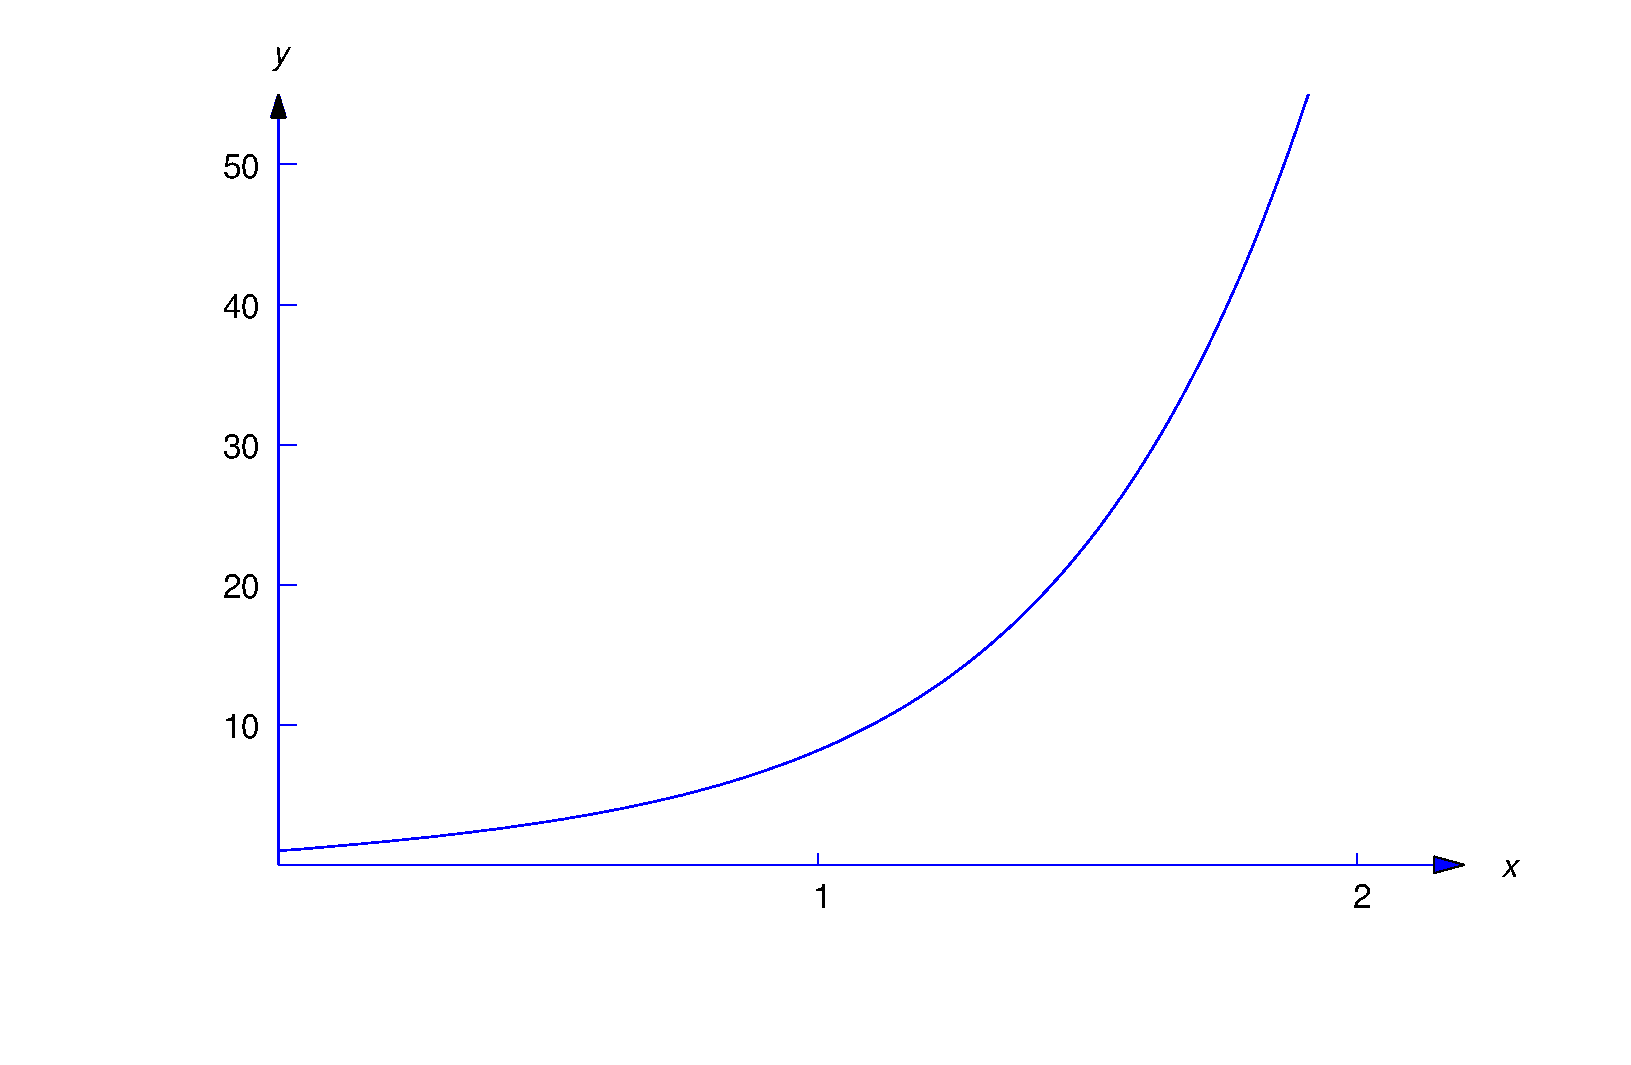
\includegraphics[bb=-78 148 689 643, width=5.67in, height=3.66in, keepaspectratio]{fig090301}
  \caption{$y_{p}=e^{x}(1+2x-x^{2}+x^{3})$ }
  \label{figure:9.3.1}
\end{figure}
\end{examplesolution}

\setcounter{example}{1}
\setcounter{equation}{3}
\begin{example}
  \label{example:9.3.2} \rm Find a particular solution of
  \begin{equation}
    \label{eq:9.3.4}y^{(4)}-y'''-6y''+4y'+8y=e^{2x}(4+19x+6x^{2}).
  \end{equation}
\end{example}
\setcounter{equation}{4}
\setcounter{figure}{1}
\begin{examplesolution}
\solution Substituting
\begin{eqnarray*}
  y       & = & ue^{2x},                   \\
  y'      & = & e^{2x}(u'+2u),             \\
  y''     & = & e^{2x}(u''+4u'+4u),        \\
  y'''    & = & e^{2x}(u'''+6u''+12u'+8u), \\
  y^{(4)} & = & e^{2x}(u^{(4)}+8u'''+24u''+32u'+16u)
\end{eqnarray*}
into \eqref{eq:9.3.4} and canceling $e^{2x}$ yields
\begin{eqnarray*}
   &  & (u^{(4)}+8u'''+24u''+32u'+16u)-(u'''+6u''+12u'+8u) \\
   &  & -6(u''+4u'+4u)+4(u'+2u)+8u=4+19x+6x^{2},
\end{eqnarray*}
or
\begin{equation}
  \label{eq:9.3.5}u^{(4)}+7u'''+12u''=4+19x+6x^{2}.
\end{equation}
Since neither $u$ nor $u'$ appear on the left, we can see that \eqref{eq:9.3.5} has a particular
solution of the form
\begin{equation}
  \label{eq:9.3.6}u_{p}=Ax^{2}+Bx^{3}+Cx^{4}.
\end{equation}
Then
\begin{eqnarray*}
  u_{p}'      & = & 2Ax+3Bx^{2}+4Cx^{3} \\
  u_{p}''     & = & 2A+6Bx+12Cx^{2}     \\
  u_{p}'''    & = & 6B+24Cx             \\
  u_{p}^{(4)} & = & 24C.
\end{eqnarray*}
Substituting $u_{p}''$, $u_{p}'''$, and $u_{p}^{(4)}$ into the left side of \eqref{eq:9.3.5} yields
\begin{eqnarray*}
  u_{p}^{(4)}+7u_{p}'''+12u_{p}'' & = & 24C+7(6B+24Cx)+12(2A+6Bx+12Cx^{2}) \\
                                  & = & (24A+42B+24C)+(72B+168C)x+144Cx^{2}.
\end{eqnarray*}
Comparing coefficients of like powers of $x$ on the right sides of this equation and
\eqref{eq:9.3.5} shows that $u_{p}$ satisfies \eqref{eq:9.3.5} if
\[
  \begin{array}{rcr}
    144C                   & = & 6\phantom{.}  \\
    72B+168C               & = & 19\phantom{.} \\
    24A+42B+\phantom{1}24C & = & 4.
  \end{array}
\]
Solving these equations successively yields $C=1/24$, $B=1/6$, $A=-1/6$. Substituting these into
\eqref{eq:9.3.6} shows that
\[
  u_{p}=\frac{x^{2}}{24}(-4+4x+x^{2})
\]
is a particular solution of \eqref{eq:9.3.5}, so
\[
  y_{p}=e^{2x}u_{p}=\frac{x^{2}e^{2x}}{24}(-4+4x+x^{2})
\]
is a particular solution of \eqref{eq:9.3.4}. (Figure~\ref{figure:9.3.2}).

\begin{figure}[H]
  \centering
  \relax
  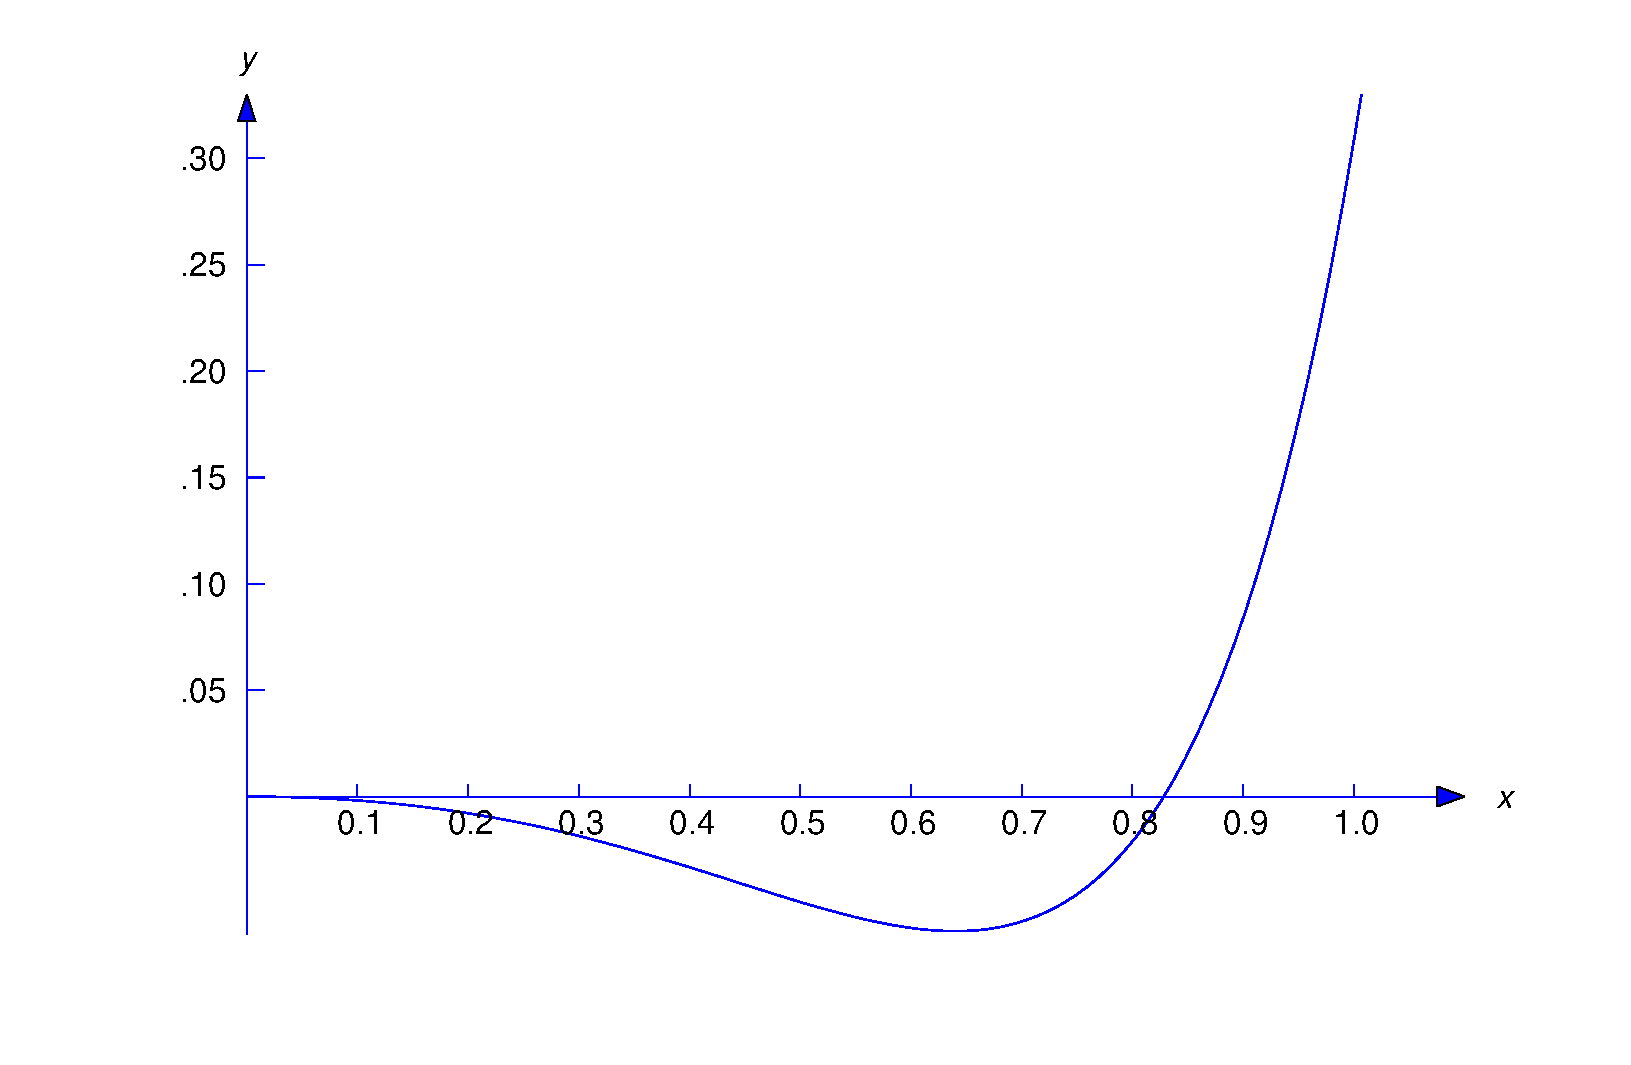
\includegraphics[bb=-78 148 689 643, width=5.67in, height=3.66in, keepaspectratio]{fig090302}
  \caption{$y_{p}=\dst{\frac{x^{2}e^{2x}}{24}(-4+4x+x^{2})}$}
  \label{figure:9.3.2}
\end{figure}
\end{examplesolution}

\setcounter{example}{2}
\setcounter{equation}{6}
\begin{example}
  \label{example:9.3.3} \rm Find a particular solution of
  \begin{equation}
    \label{eq:9.3.7}y'''+y''-4y'-4y=e^{x}[(5-5x)\cos x+(2+5x)\sin x].
  \end{equation}
\end{example}
\setcounter{equation}{7}
\setcounter{figure}{2}
\begin{examplesolution}
\solution Substituting
\begin{eqnarray*}
  y    & = & ue^{x},           \\
  y'   & = & e^{x}(u'+u),      \\
  y''  & = & e^{x}(u''+2u'+u), \\
  y''' & = & e^{x}(u'''+3u''+3u'+u)
\end{eqnarray*}
into \eqref{eq:9.3.7} and canceling $e^{x}$ yields
\[
  (u'''+3u''+3u'+u)+(u''+2u'+u)-4(u'+u)-4u =(5-5x)\cos x+(2+5x)\sin x,
\]
or
\begin{equation}
  \label{eq:9.3.8}u'''+4u''+u'-6u=(5-5x)\cos x+(2+5x)\sin x.
\end{equation}
Since $\cos x$ and $\sin x$ are not solutions of the complementary equation
\[
  u'''+4u''+u'-6u=0,
\]
a theorem analogous to Theorem~5.5.1 implies that \eqref{eq:9.3.8} has a particular
solution of the form
\begin{equation}
  \label{eq:9.3.9}u_{p}=(A_{0}+A_{1}x)\cos x+(B_{0}+B_{1}x)\sin x.
\end{equation}
Then
\begin{eqnarray*}
  u_{p}'=(A_{1}+B_{0}+B_{1}x)\cos x+(B_{1}-A_{0}-A_{1}x)\sin x,\\ u_{p}''=(2B_{1}-A_{0}-A_{1}x)\cos x-(2A_{1}+B_{0}+B_{1}x)\sin x,\\ u_{p}'''=-(3A_{1}+B_{0}+B_{1}x)\cos x-(3B_{1}-A_{0}-A_{1}x)\sin x,\\
\end{eqnarray*}
so
\[
  \begin{array}{rcl}
    u_{p}'''+4u_{p}''+u_{p}'-6u_{p} & = & -\left[10A_{0}+2A_{1}-8B_{1}+10A_{1}x\right]\cos x  \\
                                    &   & -\left[10B_{0}+2B_{1}+8A_{1}+10B_{1}x\right]\sin x.
  \end{array}
\]
Comparing the coefficients of $x\cos x$, $x\sin x$, $\cos x$, and $\sin x$ here with the
corresponding coefficients in \eqref{eq:9.3.8} shows that $u_{p}$ is a solution of \eqref{eq:9.3.8}
if
\[
  \begin{array}{rcr}
    -10A_{1}               & = & -5\phantom{.}           \\
    -10B_{1}               & = & \phantom{-}5\phantom{.} \\
    -10A_{0}-2A_{1}+8B_{1} & = & 5\phantom{.}            \\
    -10B_{0}-2B_{1}-8A_{1} & = & 2.
  \end{array}
\]
Solving the first two equations yields $A_{1}=1/2$, $B_{1}=-1/2$. Substituting these into the last
two equations yields
\begin{eqnarray*}
  -10A_{0} & = & 5+2A_{1}-8B_{1}=10\phantom{.} \\
  -10B_{0} & = & 2+2B_{1}+8A_{1}=5,
\end{eqnarray*}
so $A_{0}=-1$, $B_{0}=-1/2$. Substituting $A_{0}=-1$, $A_{1}=1/2$, $B_{0}=-1/2$, $B_{1}=-1/2$ into
\eqref{eq:9.3.9} shows that
\[
  u_{p}=-\dst\frac{1}{2}\left[(2-x)\cos x+(1+x)\sin x\right]
\]
is a particular solution of \eqref{eq:9.3.8}, so
\[
  y_{p}=e^{x}u_{p}=-\frac{e^{x}}{2}\left[(2-x)\cos x+(1+x)\sin x\right]
\]
is a particular solution of \eqref{eq:9.3.7} (Figure~\ref{figure:9.3.3}).

\begin{figure}[H]
  \centering
  \relax
  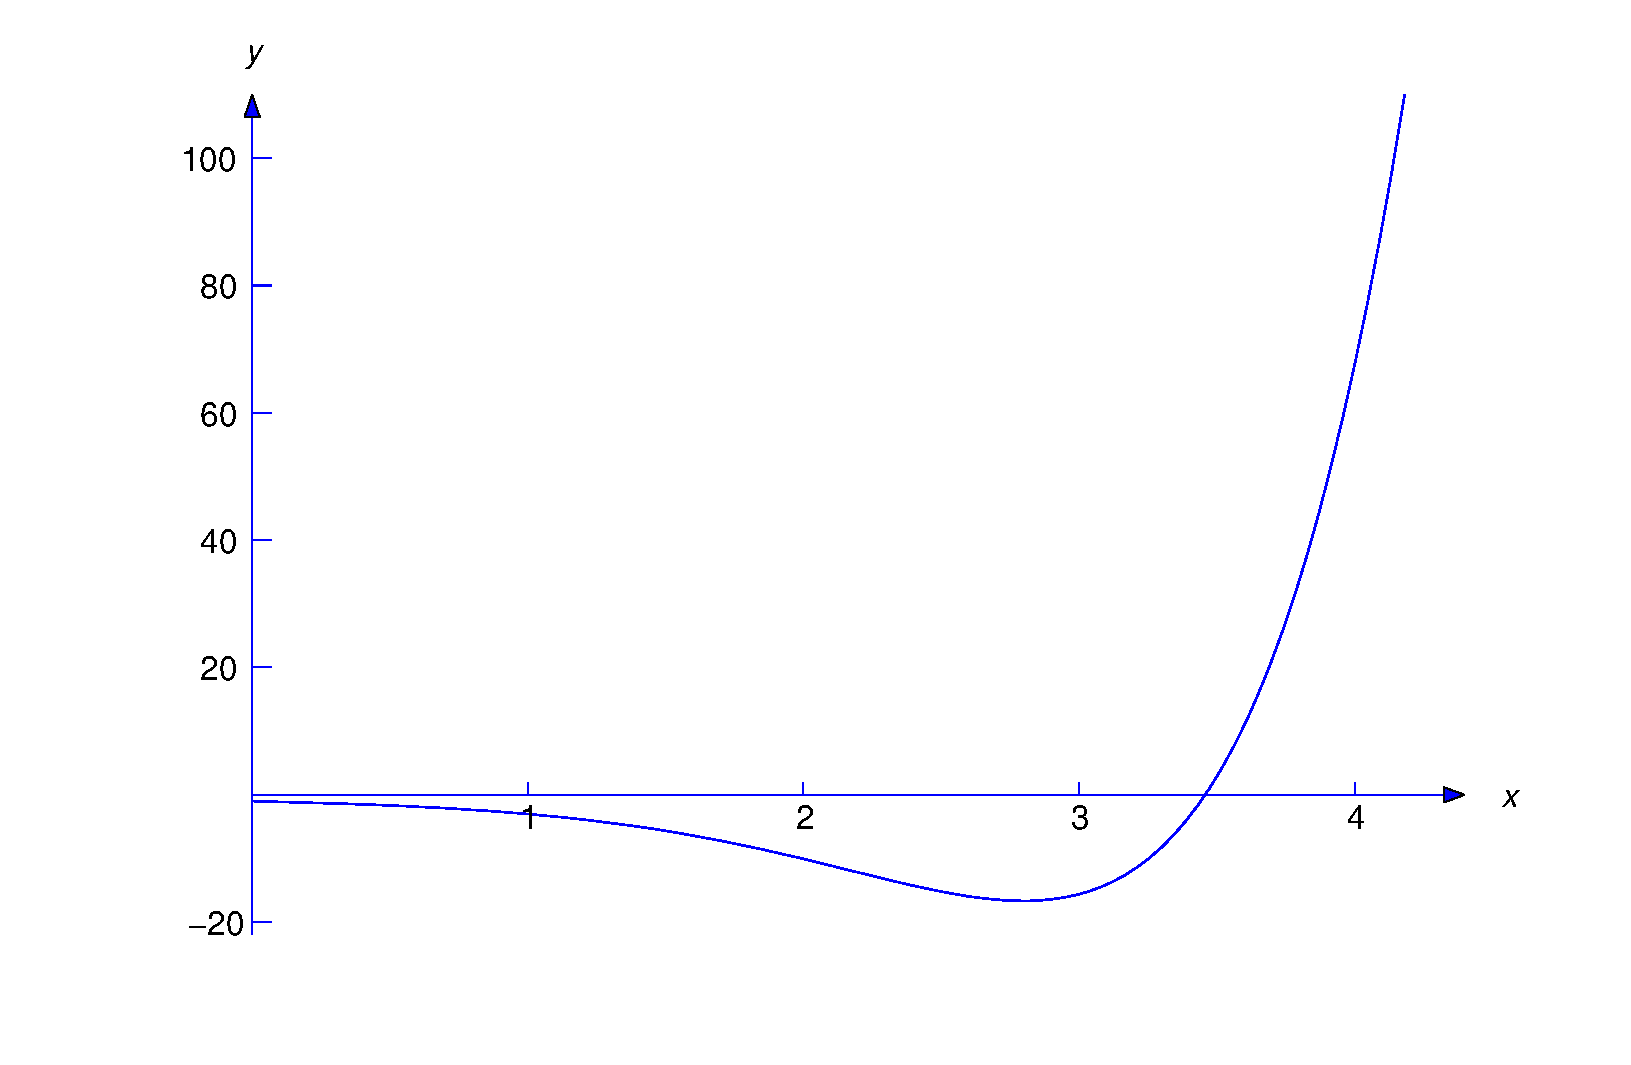
\includegraphics[bb=-78 148 689 643, width=5.67in, height=3.66in, keepaspectratio]{fig090303}
  \caption{$y_{p}=\dst{e^{x}u_{p}=-\frac{e^{x}}{2}\left[(2-x)\cos x+(1+x)\sin x\right]}$}
  \label{figure:9.3.3}
\end{figure}
\end{examplesolution}

\setcounter{example}{3}
\setcounter{equation}{9}
\begin{example}
  \label{example:9.3.4} \rm Find a particular solution of
  \begin{equation}
    \label{eq:9.3.10}y'''+4y''+6y'+4y= e^{-x}\left[(1-6x)\cos x-(3+2x)\sin x\right].
  \end{equation}
\end{example}
\setcounter{equation}{10}
\setcounter{figure}{3}
\begin{examplesolution}
\solution Substituting
\begin{eqnarray*}
  y    & = & ue^{-x},           \\
  y'   & = & e^{-x}(u'-u),      \\
  y''  & = & e^{-x}(u''-2u'+u), \\
  y''' & = & e^{-x}(u'''-3u''+3u'-u)
\end{eqnarray*}
into \eqref{eq:9.3.10} and canceling $e^{-x}$ yields
\[
  (u'''-3u''+3u'-u)+4(u''-2u'+u)+6(u'-u)+4u =(1-6x)\cos x-(3+2x)\sin x,
\]
or
\begin{equation}
  \label{eq:9.3.11}u'''+u''+u'+u=(1-6x)\cos x-(3+2x)\sin x.
\end{equation}
Since $\cos x$ and $\sin x$ are solutions of the complementary equation
\[
  u'''+u''+u'+u=0,
\]
a theorem analogous to Theorem~5.5.1 implies that \eqref{eq:9.3.11} has a particular
solution of the form
\begin{equation}
  \label{eq:9.3.12}u_{p}=(A_{0}x+A_{1}x^{2})\cos x+(B_{0}x+B_{1}x^{2})\sin x.
\end{equation}
\newpage

Then
\begin{eqnarray*}
  u_{p}'   & = & [A_{0}+(2A_{1}+B_{0})x+B_{1}x^{2}]\cos x+[B_{0}+(2B_{1}-A_{0})x-A_{1}x^{2}]\sin x, \\
  u_{p}''  & = & [2A_{1}+2B_{0}-(A_{0}-4B_{1})x-A_{1}x^{2}]\cos x                                   \\
           &   & +[2B_{1}-2A_{0}-(B_{0}+4A_{1})x-B_{1}x^{2}]\sin x,                                 \\
  u_{p}''' & = & -[3A_{0}-6B_{1}+(6A_{1}+B_{0})x+B_{1}x^{2}]\cos x                                  \\
           &   & -[3B_{0}+6A_{1}+(6B_{1}-A_{0})x-A_{1}x^{2}]\sin x,
\end{eqnarray*}
so
\[
  \begin{array}{rcl}
    u_{p}'''+u_{p}''+u_{p}'+u_{p} & = & -[2A_{0}-2B_{0}-2A_{1}-6B_{1}+(4A_{1}-4B_{1})x]\cos x  \\
                                  &   & -[2B_{0}+2A_{0}-2B_{1}+6A_{1}+(4B_{1}+4A_{1})x]\sin x.
  \end{array}
\]
Comparing the coefficients of $x\cos x$, $x\sin x$, $\cos x$, and $\sin x$ here with the
corresponding coefficients in \eqref{eq:9.3.11} shows that $u_{p}$ is a solution of
\eqref{eq:9.3.11} if
\[
  \begin{array}{rcr}
    -4A_{1}+4B_{1}               & = & -6\phantom{.}           \\
    -4A_{1}-4B_{1}               & = & -2\phantom{.}           \\
    -2A_{0}+2B_{0}+2A_{1}+6B_{1} & = & \phantom{-}1\phantom{.} \\
    -2A_{0}-2B_{0}-6A_{1}+2B_{1} & = & -3.
  \end{array}
\]
Solving the first two equations yields $A_{1}=1$, $B_{1}=-1/2$. Substituting these into the last two
equations yields
\begin{eqnarray*}
  -2A_{0}+2B_{0} & = & \phantom{-}1-2A_{1}-6B_{1}=2\phantom{.} \\
  -2A_{0}-2B_{0} & = & -3+6A_{1}-2B_{1}=4,
\end{eqnarray*}

\begin{figure}[H]
  \centering
  \relax
  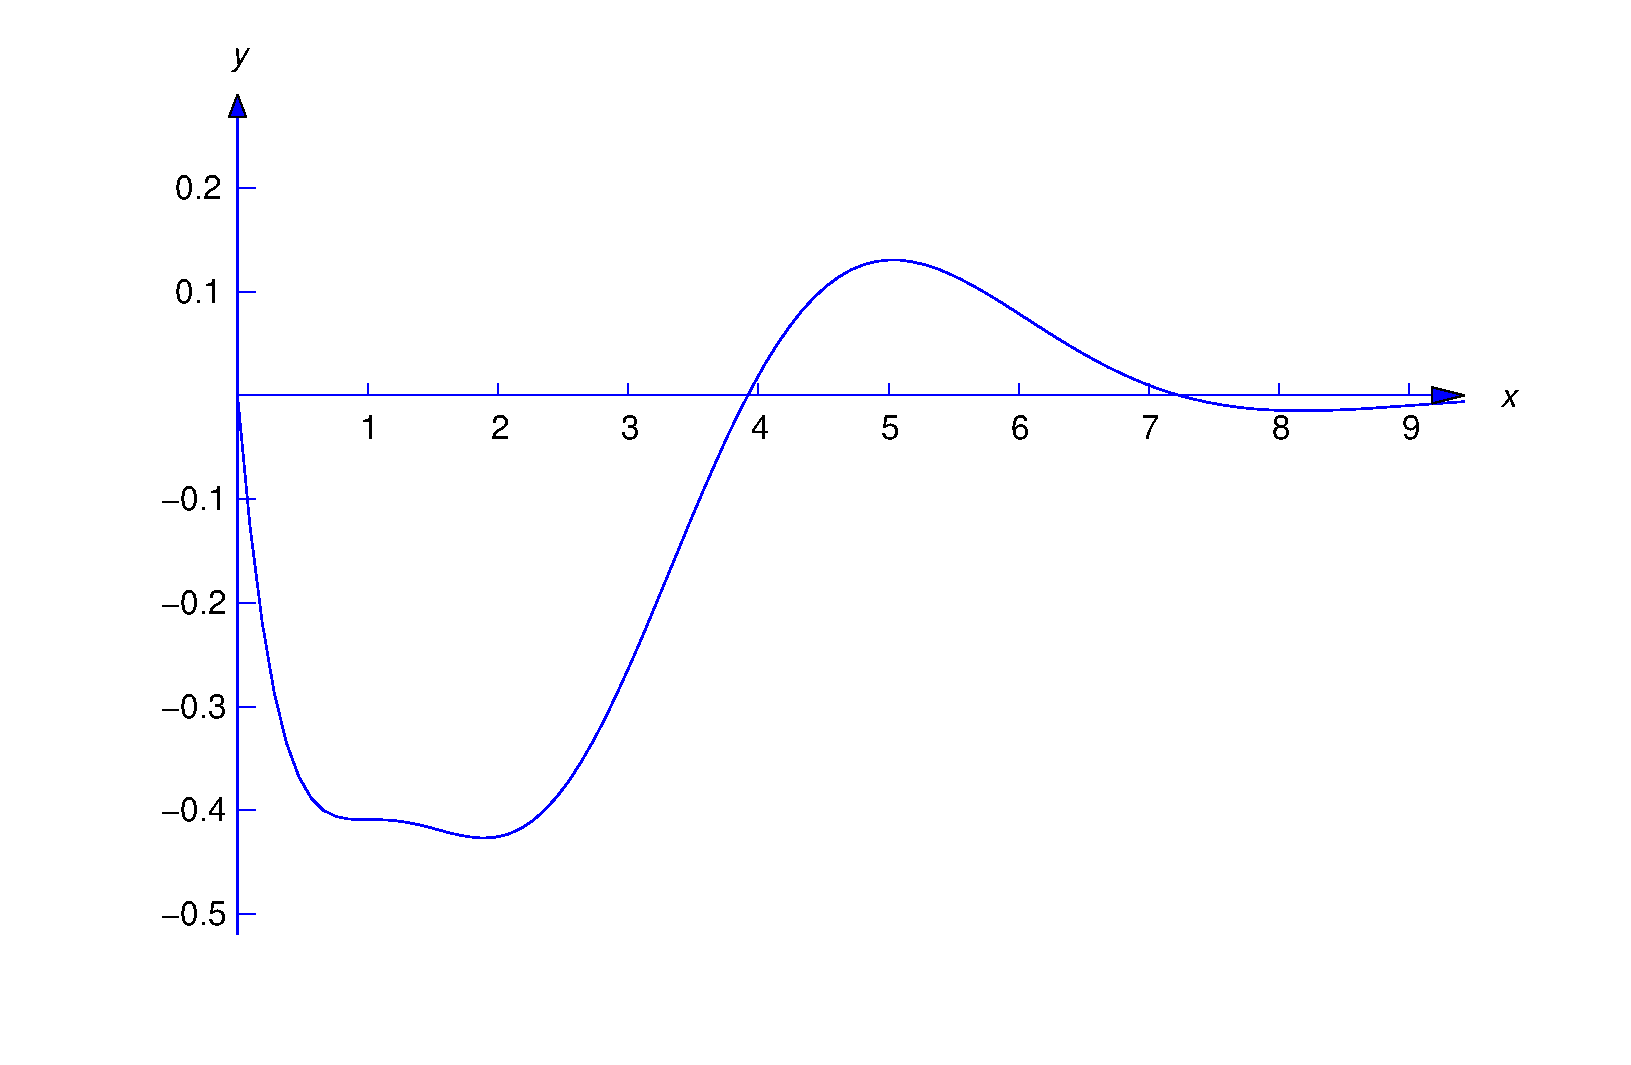
\includegraphics[bb=-78 148 689 643, width=5.67in, height=3.66in, keepaspectratio]{fig090304}
  \caption{$\dst{y_{p}=-\frac{xe^{-x}}{2}\left[(3-2x)\cos x+(1+x)\sin x\right]}$}
  \label{figure:9.3.4}
\end{figure}

\noindent
so $A_{0}=-3/2$ and $B_{0}=-1/2$. Substituting $A_{0}=-3/2$, $A_{1}=1$, $B_{0}=-1/2$, $B_{1}=-1/2$
into \eqref{eq:9.3.12} shows that
\[
  u_{p}=-\dst\frac{x}{2}\left[(3-2x)\cos x+(1+x)\sin x\right]
\]
is a particular solution of \eqref{eq:9.3.11}, so
\[
  y_{p}=e^{-x}u_{p}=-\frac{xe^{-x}}{2}\left[(3-2x)\cos x+(1+x)\sin x\right]
\]
(Figure~\ref{figure:9.3.4}) is a particular solution of \eqref{eq:9.3.10}.
\end{examplesolution}

\section*{Section 9.4}
\setcounter{chapter}{9}
\setcounter{section}{4}

\setcounter{example}{0}
\setcounter{equation}{7}
\begin{example}
  \label{example:9.4.1} \rm Find a particular solution of
  \begin{equation}
    \label{eq:9.4.8}xy'''-y''-xy'+y=8x^{2}e^{x},
  \end{equation}
  given that $y_{1}=x$, $y_{2}=e^{x}$, and $y_{3}=e^{-x}$ form a fundamental set of solutions of the
  complementary equation. Then find the general solution of \eqref{eq:9.4.8}.
\end{example}
\begin{examplesolution}
\solution We seek a particular solution of \eqref{eq:9.4.8} of the form
\[
  y_{p}=u_{1}x+u_{2}e^{x}+u_{3}e^{-x}.
\]
The Wronskian of $\{y_{1},y_{2},y_{3}\}$ is
\[
  W(x)=\left|
  \begin{array}{ccr}
    x & e^{x} & e^{-x}  \\
    1 & e^{x} & -e^{-x} \\
    0 & e^{x} & e^{-x}
  \end{array}\right|,
\]
so
\begin{eqnarray*}
  W_{1}&=& \left|
  \begin{array}{cr}
    e^{x} & e^{-x}  \\
    e^{x} & -e^{-x}
  \end{array}\right|=-2,\\[10pt] W_{2}&=& \left|
  \begin{array}{cr}
    x & e^{-x}  \\
    1 & -e^{-x}
  \end{array}\right|=-e^{-x}(x+1),\\ W_{3}&=& \left|
  \begin{array}{cc}
    x & e^{x} \\
    1 & e^{x}
  \end{array}\right|=e^{x}(x-1).
\end{eqnarray*}
Expanding $W$ by cofactors of the last row yields
\[
  W=0W_{1}-e^{x}W_{2}+e^{-x}W_{3}=0(-2)-e^{x}\left(-e^{-x}(x+1)\right) +e^{-x}e^{x}(x-1)=2x.
\]
Since $F(x)=8x^{2}e^{x}$ and $P_{0}(x)=x$,
\[
  \frac{F}{P_{0}W}=\frac{8x^{2}e^{x}}{x\cdot2x}=4e^{x}.
\]
Therefore, from \textup{(9.4.7)}
\begin{eqnarray*}
  u'_{1} & = & \phantom{-}4e^{x}W_{1}=\phantom{-}4e^{x}(-2)=-8e^{x}, \\
  u_{2}' & = & -4e^{x}W_{2}=-4e^{x}\left(-e^{-x}(x+1)\right)=4(x+1), \\
  u_{3}' & = & \phantom{-}4e^{x}W_{3}=\phantom{-}4e^{x}\left(e^{x}(x-1)\right)=4e^{2x}(x-1).
\end{eqnarray*}
Integrating and taking the constants of integration to be zero yields
\[
  u_{1}=-8e^{x},\quad u_{2}=2(x+1)^{2},u_{3}=e^{2x}(2x-3).
\]
Hence,
\begin{eqnarray*}
  y_{p} & = & u_{1}y_{1}+u_{2}y_{2}+u_{3}y_{3}                             \\
        & = & (-8e^{x})x+e^{x}(2(x+1)^{2})+e^{-x}\left(e^{2x}(2x-3)\right) \\
        & = & e^{x}(2x^{2}-2x-1).
\end{eqnarray*}
Since $-e^{x}$ is a solution of the complementary equation, we redefine
\[
  y_{p}=2xe^{x}(x-1).
\]
Therefore the general solution of \eqref{eq:9.4.8} is
\[
  y=2xe^{x}(x-1)+c_{1}x+c_{2}e^{x}+c_{3}e^{-x}.
\]
\end{examplesolution}

\setcounter{example}{1}
\setcounter{equation}{9}
\begin{example}
  \label{example:9.4.2} \rm Find a particular solution of
  \begin{equation}
    \label{eq:9.4.10}x^{4}y^{(4)}+6x^{3}y'''+2x^{2}y''-4xy'+4y=12x^{2},
  \end{equation}
  given that $y_{1}=x$, $y_{2}=x^{2}$, $y_{3}=1/x$ and $y_{4}=1/x^{2}$ form a fundamental set of
  solutions of the complementary equation. Then find the general solution of \eqref{eq:9.4.10} on
  $(-\infty,0)$ and $(0,\infty)$.
\end{example}
\begin{examplesolution}
\solution We seek a particular solution of \eqref{eq:9.4.10} of the form
\[
  y_{p}=u_{1}x+u_{2}x^{2}+\frac{u_{3}}{x}+\frac{u_{4}}{x^{2}}.
\]
The Wronskian of $\{y_{1},y_{2},y_{3},y_{4}\}$ is
\[
  W(x)=\left|
  \begin{array}{cccr}
    x & x^{2} & 1/x      & 1/x^{2}   \\[5pt]
    1 & 2x    & -1/x^{2} & -2/x^{3}  \\[5pt]
    0 & 2     & 2/x^{3}  & 6/x^{4}   \\[5pt]
    0 & 0     & -6/x^{4} & -24/x^{5}
  \end{array}\right|,
\]
so
\begin{eqnarray*}
  W_{1}&=& \left|
  \begin{array}{ccr}
    x^{2} & 1/x      & 1/x^{2}  \\[5pt]
    2x    & -1/x^{2} & -2/x^{3} \\[5pt]
    2     & 2/x^{3}  & 6/x^{4}
  \end{array}\right|=-\frac{12}{x^{4}},\\[10pt] W_{2}&=& \left|
  \begin{array}{ccr}
    x & 1/x      & 1/x^{2}  \\[5pt]
    1 & -1/x^{2} & -2/x^{3} \\[5pt]
    0 & 2/x^{3}  & 6/x^{4}
  \end{array}\right|=-\frac{6}{x^{5}},\\[10pt] W_{3}&=& \left|
  \begin{array}{ccc}
    x & x^{2} & 1/x^{2}  \\[5pt]
    1 & 2x    & -2/x^{3} \\[5pt]
    0 & 2     & 6/x^{4}
  \end{array}\right|=\frac{12}{x^{2}},\\ W_{4}&=& \left|
  \begin{array}{ccc}
    x & x^{2} & 1/x      \\[5pt]
    1 & 2x    & -1/x^{2} \\[5pt]
    0 & 2     & 2/x^{3}
  \end{array}\right|=\frac{6}{x}.
\end{eqnarray*}
Expanding $W$ by cofactors of the last row yields
\begin{eqnarray*}
  W & = & -0W_{1}+0W_{2}-\left(-\frac{6}{x^{4}}\right)W_{3}+\left(-\frac{24}{x^{5}}\right)W_{4} \\
    & = & \frac{6}{x^{4}}\frac{12}{x^{2}}-\frac{24}{x^{5}}\frac{6}{x}=-\frac{72}{x^{6}}.
\end{eqnarray*}
Since $F(x)=12x^{2}$ and $P_{0}(x)=x^{4}$,
\[
  \frac{F}{P_{0}W}=\frac{12x^{2}}{x^{4}}\left(-\frac{x^{6}}{72}\right)=-\frac{x^{4}}{6}.
\]
Therefore, from \textup{(9.4.9)},
\begin{eqnarray*}
  u'_{1} & = & -\left(-\frac{x^{4}}{6}\right)W_{1}=\frac{x^{4}}{6}\left(-\frac{12}{x^{4}}\right)=-2,       \\[5pt]
  u_{2}' & = & \phantom{-}-\frac{x^{4}}{6}W_{2}=-\frac{x^{4}}{6}\left(-\frac{6}{x^{5}}\right)=\frac{1}{x}, \\[5pt]
  u_{3}' & = & -\left(-\frac{x^{4}}{6}\right)W_{3}=\frac{x^{4}}{6}\frac{12}{x^{2}}=2x^{2},                 \\
  u_{4}' & = & \phantom{-}-\frac{x^{4}}{6}W_{4}=-\frac{x^{4}}{6}\frac{6}{x}=-x^{3}.
\end{eqnarray*}
Integrating these and taking the constants of integration to be zero yields
\[
  u_{1}=-2x,\quad u_{2}=\ln|x|,\quad u_{3}=\frac{2x^{3}}{3}, u_{4}=-\frac{x^{4}}{4}.
\]
Hence,
\begin{eqnarray*}
  y_{p} & = & u_{1}y_{1}+u_{2}y_{2}+u_{3}y_{3}+u_{4}y_{4}                                                   \\
        & = & (-2x)x+(\ln|x|)x^{2}+\frac{2x^{3}}{3}\frac{1}{x}+\left(-\frac{x^{4}}{4}\right)\frac{1}{x^{2}} \\
        & = & x^{2}\ln|x|-\frac{19x^{2}}{12}.
\end{eqnarray*}
Since $-19x^{2}/12$ is a solution of the complementary equation, we redefine
\[
  y_{p}=x^{2}\ln|x|.
\]
Therefore
\[
  y=x^{2}\ln|x|+c_{1}x+c_{2}x^{2}+\frac{c_{3}}{x}+\frac{c_{4}}{x^{2}}
\]
is the general solution of \eqref{eq:9.4.10} on $(-\infty,0)$ and $(0,\infty)$.
\end{examplesolution}

\section*{Section 10.1}
\phantomsection
\addcontentsline{toc}{chapter}{Chapter 10}
\setcounter{chapter}{10}
\setcounter{section}{1}

\setcounter{example}{0}
\begin{example}
  \label{example:10.1.1} \rm Tanks $T_{1}$ and $T_{2}$ contain 100 gallons and 300 gallons of salt
  solutions, respectively. Salt solutions are simultaneously added to both tanks from external
  sources, pumped from each tank to the other, and drained from both tanks
  (Figure~10.1.1). A solution with $1$ pound of salt per gallon is pumped into $T_{1}$
  from an external source at $5$~gal/min, and a solution with $2$ pounds of salt per gallon is
  pumped into $T_{2}$ from an external source at $4$~gal/min. The solution from $T_{1}$ is pumped
  into $T_{2}$ at 2 gal/min, and the solution from $T_{2}$ is pumped into $T_{1}$ at $3$ gal/min.
  $T_{1}$ is drained at $6$~gal/min and $T_{2}$ is drained at 3~gal/min. Let $Q_{1}(t)$ and
  $Q_{2}(t)$ be the number of pounds of salt in $T_{1}$ and $T_{2}$, respectively, at time $t>0$.
  Derive a system of differential equations for $Q_{1}$ and $Q_{2}$. Assume that both mixtures are
  well stirred.
\end{example}
\setcounter{equation}{0}
\begin{examplesolution}
\solution As in Section~4.2, let {\relax\it rate in\/} and {\relax\it rate out\/} denote
the rates (lb/min) at which salt enters and leaves a tank; thus,
\begin{eqnarray*}
  Q_{1}' & = & (\mbox{rate in})_{1}-(\mbox{rate out})_{1}, \\[2\jot]
  Q_{2}' & = & (\mbox{rate in})_{2}-(\mbox{rate out})_{2}.
\end{eqnarray*}
Note that the volumes of the solutions in $T_{1}$ and $T_{2}$ remain constant at 100~gallons and
300~gallons, respectively.

$T_{1}$ receives salt from the external source at the rate of
\[
  \mbox{(1 lb/gal) }\times\mbox{ (5~gal/min)}=\mbox{ 5 lb/min},
\]
and from $T_{2}$ at the rate of
\[
  \mbox{(lb/gal in }T_{2})\times\mbox{ (3~gal/min) }=\frac{1}{300}Q_{2}\times3\\[2\jot]=\frac{1}{100}Q_{2}\mbox{ lb/min}.
\]
Therefore
\begin{equation}
  \label{eq:10.1.1}\mbox{(rate in)}_{1}=5+\frac{1}{100}Q_{2}.
\end{equation}
Solution leaves $T_{1}$ at the rate of 8~gal/min, since 6~gal/min are drained and 2~gal/min are
pumped to $T_{2}$; hence,
\begin{equation}
  \label{eq:10.1.2}(\mbox{rate out})_{1}=(\mbox{ lb/gal in T}_{1})\times\mbox{(8~gal/min) }=\frac{1}{100}Q_{1}\times8=\frac{2}{25}Q_{1}.
\end{equation}
Eqns.~\eqref{eq:10.1.1} and \eqref{eq:10.1.2} imply that
\begin{equation}
  \label{eq:10.1.3}Q_{1}'=5+\frac{1}{100}Q_{2}-\frac{2}{25}Q_{1}.
\end{equation}

$T_{2}$ receives salt from the external source at the rate of
\[
  \mbox{(2 lb/gal) }\times\mbox{ (4~gal/min)}=\mbox{ 8 lb/min},
\]
and from $T_{1}$ at the rate of
\[
  \mbox{(lb/gal in }T_{1})\times\mbox{ (2~gal/min) }=\frac{1}{100}Q_{1}\times2\\[2\jot]=\frac{1}{50}Q_{1}\mbox{ lb/min}.
\]
Therefore
\begin{equation}
  \label{eq:10.1.4}\mbox{(rate in)}_{2}=8+\frac{1}{50}Q_{1}.
\end{equation}
Solution leaves $T_{2}$ at the rate of $6$~gal/min, since $3$~gal/min are drained and $3$~gal/min
are pumped to $T_{1}$; hence,
\begin{equation}
  \label{eq:10.1.5}(\mbox{rate out})_{2}=(\mbox{ lb/gal in T}_{2})\times\mbox{(6~gal/min) }=\frac{1}{300}Q_{2}\times6=\frac{1}{50}Q_{2}.
\end{equation}
Eqns.~\eqref{eq:10.1.4} and \eqref{eq:10.1.5} imply that
\begin{equation}
  \label{eq:10.1.6}Q_{2}'=8+\frac{1}{50}Q_{1}-\frac{1}{50}Q_{2}.
\end{equation}

We say that \eqref{eq:10.1.3} and \eqref{eq:10.1.6} form a {\relax\it system of two first
order equations in two unknowns\/}, and write them together as
\begin{eqnarray*}
  Q_{1}' & = & \dst{5-\frac{2}{25}Q_{1}+\frac{1}{100}Q_{2}} \\
  Q_{2}' & = & \dst{8+\frac{1}{50}Q_{1}-\frac{1}{50}Q_{2}}.\quad\bbox
\end{eqnarray*}
\end{examplesolution}

\setcounter{example}{1}
\begin{example}
  \label{example:10.1.2} \rm A mass $m_{1}$ is suspended from a rigid support on a spring $S_{1}$
  and a second mass $m_{2}$ is suspended from the first on a spring $S_{2}$
  (Figure~\ref{figure:10.1.2}). The springs obey Hooke's law, with spring constants $k_{1}$ and
  $k_{2}$. Internal friction causes the springs to exert damping forces proportional to the rates of
  change of their lengths, with damping constants $c_{1}$ and $c_{2}$. Let $y_{1}=y_{1}(t)$ and
  $y_{2}=y_{2}(t)$ be the displacements of the two masses from their equilibrium positions at time
  $t$, measured positive upward. Derive a system of differential equations for $y_{1}$ and $y_{2}$,
  assuming that the masses of the springs are negligible and that vertical external forces $F_{1}$
  and $F_{2}$ also act on the objects.
\end{example}
\setcounter{equation}{6}
\setcounter{figure}{1}
\begin{examplesolution}
\solution In equilibrium, $S_{1}$ supports both $m_{1}$ and $m_{2}$ and $S_{2}$ supports only
$m_{2}$. Therefore, if $\Delta\ell_{1}$ and $\Delta\ell_{2}$ are the elongations of the springs in
equilibrium then
\begin{equation}
  \label{eq:10.1.7}(m_{1}+m_{2})g=k_{1}\Delta\ell_{1}\quad\mbox{ and }\quad m_{2}g=k_{2}\Delta\ell_{2}.
\end{equation}

\begin{figure}[H]
  \centering
  \relax
  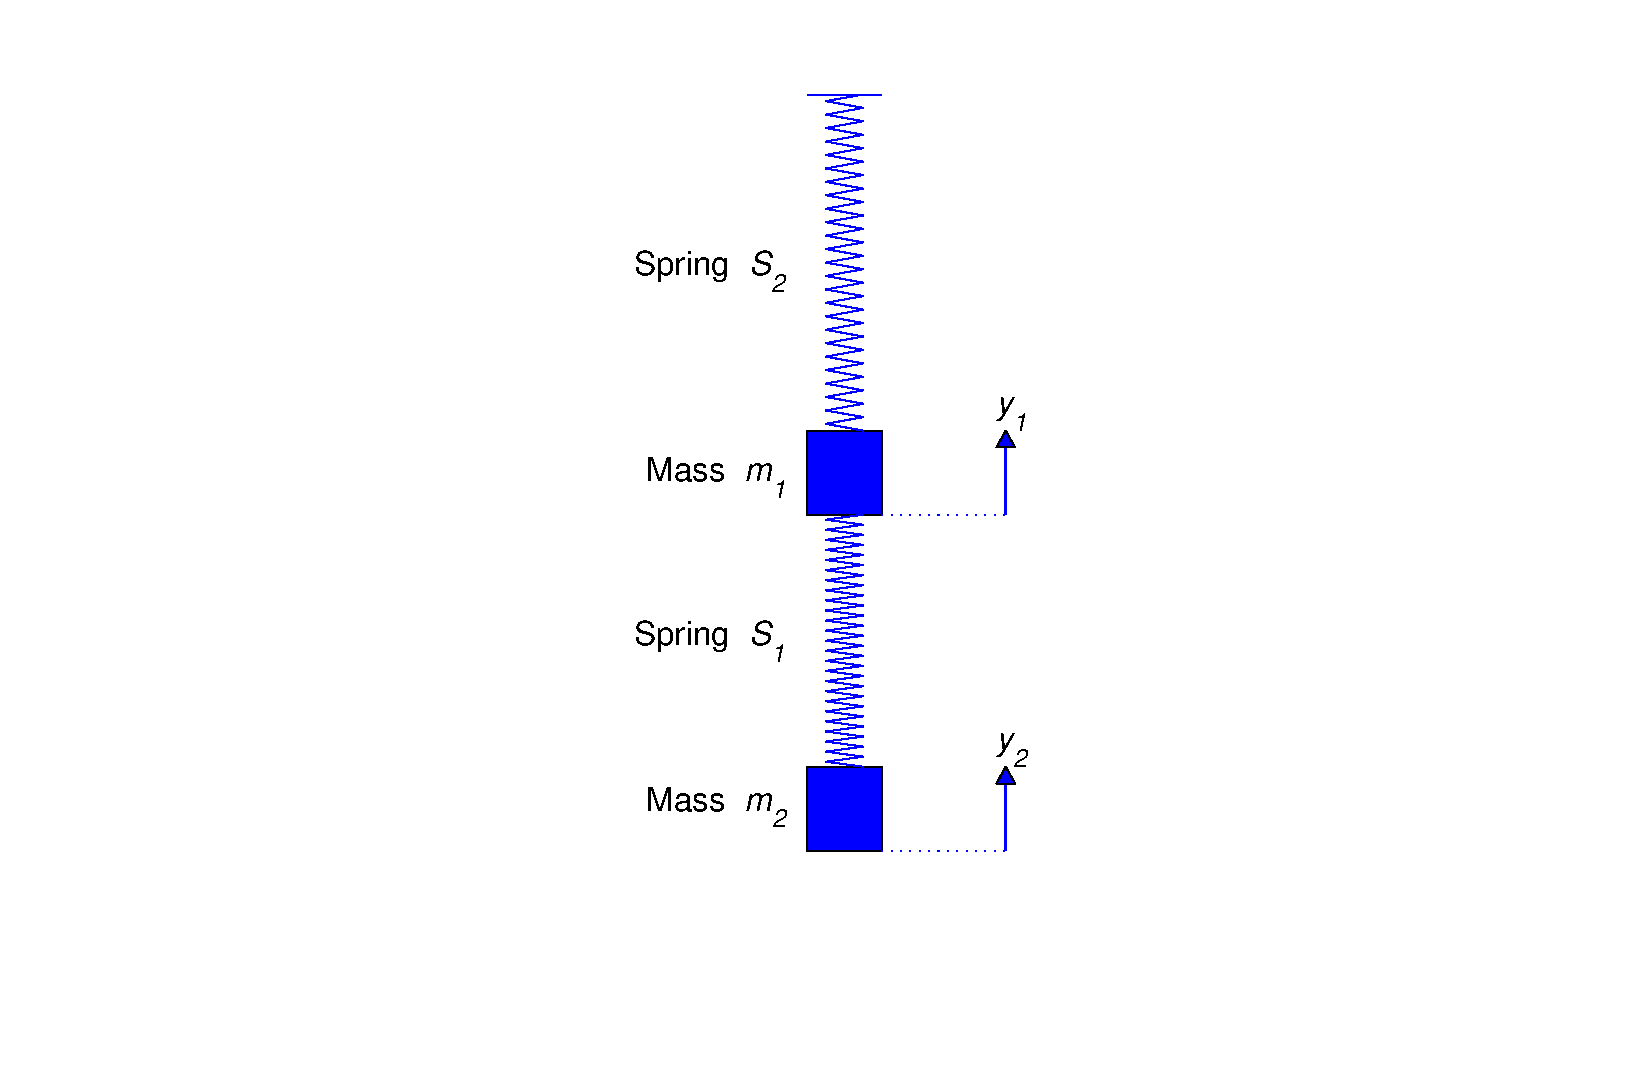
\includegraphics[bb=-78 148 689 643, width=5.67in, height=3.66in, keepaspectratio]{fig100102}
  \caption{}
  \label{figure:10.1.2}
\end{figure}

Let $H_{1}$ be the Hooke's law force acting on $m_{1}$, and let $D_{1}$ be the damping force on
$m_{1}$. Similarly, let $H_{2}$ and $D_{2}$ be the Hooke's law and damping forces acting on $m_{2}$.
According to Newton's second law of motion,
\begin{equation}
  \label{eq:10.1.8}
  \begin{array}{ccl}
    m_{1}y_{1}''=-m_{1}g+H_{1}+D_{1}+F_{1}, \\[1\jot]
    m_{2}y_{2}''=-m_{2}g+H_{2}+D_{2}+F_{2}.
  \end{array}
\end{equation}
When the displacements are $y_{1}$ and $y_{2}$, the change in length of $S_{1}$ is
$-y_{1}+\Delta\ell_{1}$ and the change in length of $S_{2}$ is $-y_{2}+y_{1}+\Delta\ell_{2}$. Both
springs exert Hooke's law forces on $m_{1}$, while only $S_{2}$ exerts a Hooke's law force on
$m_{2}$. These forces are in directions that tend to restore the springs to their natural lengths.
Therefore
\begin{equation}
  \label{eq:10.1.9}H_{1}=k_{1}(-y_{1}+\Delta\ell_{1})-k_{2}(-y_{2}+y_{1}+\Delta\ell_{2})\quad\mbox{ and }\quad H_{2}=k_{2}(-y_{2}+y_{1}+\Delta\ell_{2}).
\end{equation}
When the velocities are $y_{1}'$ and $y_{2}'$, $S_{1}$ and $S_{2}$ are changing length at the rates
$-y_{1}'$ and $-y_{2}'+y_{1}'$, respectively. Both springs exert damping forces on $m_{1}$, while
only $S_{2}$ exerts a damping force on $m_{2}$. Since the force due to damping exerted by a spring
is proportional to the rate of change of length of the spring and in a direction that opposes the
change, it follows that
\begin{equation}
  \label{eq:10.1.10}D_{1}=-c_{1}y_{1}'+c_{2}(y_{2}'-y_{1}')\quad\mbox{ and }\quad D_{2}=-c_{2}(y_{2}'-y_{1}').
\end{equation}

From \eqref{eq:10.1.8}, \eqref{eq:10.1.9}, and \eqref{eq:10.1.10},
\begin{equation}
  \label{eq:10.1.11}
  \begin{array}{ccl}
    m_{1}y_{1}'' & =       & -m_{1}g+k_{1}(-y_{1}+\Delta\ell_{1})-k_{2}(-y_{2}+y_{1}+\Delta\ell_{2})         \\[1\jot]
                 & \mbox{} & -c_{1}y_{1}'+c_{2}(y_{2}'-y_{1}')+F_{1}                                         \\[1\jot]
                 & =       & -(m_{1}g-k_{1}\Delta\ell_{1}+k_{2}\Delta\ell_{2})-k_{1}y_{1}+k_{2}(y_{2}-y_{1}) \\[1\jot]
                 & \mbox{} & -c_{1}y_{1}'+c_{2}(y_{2}'-y_{1}')+F_{1}
  \end{array}
\end{equation}
and
\begin{equation}
  \label{eq:10.1.12}
  \begin{array}{ccl}
    m_{2}y_{2}'' & = & -m_{2}g+k_{2}(-y_{2}+y_{1}+\Delta\ell_{2})-c_{2}(y_{2}'-y_{1}')+F_{2}        \\[1\jot]
                 & = & -(m_{2}g-k_{2}\Delta\ell_{2})-k_{2}(y_{2}-y_{1})-c_{2}(y_{2}'-y_{1}')+F_{2}.
  \end{array}
\end{equation}
From \eqref{eq:10.1.7},
\[
  m_{1}g-k_{1}\Delta\ell_{1}+k_{2}\Delta\ell_{2}=-m_{2}g+k_{2}\Delta\ell_{2}=0.
\]
Therefore we can rewrite \eqref{eq:10.1.11} and \eqref{eq:10.1.12} as
\begin{eqnarray*}
  m_{1}y_{1}'' & = & -(c_{1}+c_{2})y_{1}'+c_{2}y_{2}'-(k_{1}+k_{2})y_{1}+k_{2}y_{2}+F_{1} \\
  m_{2}y_{2}'' & = & c_{2}y_{1}'-c_{2}y_{2}'+k_{2}y_{1}-k_{2}y_{2}+F_{2}.\quad\bbox
\end{eqnarray*}
\end{examplesolution}

\setcounter{example}{2}
\setcounter{equation}{12}
\begin{example}
  \label{example:10.1.3} \rm Let ${\bf X}={\bf X}(t)=x(t)\,{\bf i}+y(t)\,{\bf j}+z(t)\,{\bf k}$ be
  the position vector at time $t$ of an object with mass $m$, relative to a rectangular coordinate
  system with origin at Earth's center (Figure~10.1.3). According to Newton's law of
  gravitation, Earth's gravitational force ${\bf F}={\bf F}(x,y,z)$ on the object is inversely
  proportional to the square of the distance of the object from Earth's center, and directed toward
  the center; thus,
  \begin{equation}
    \label{eq:10.1.13}{\bf F}=\frac{K}{\|{\bf X}\|^{2}}\left(-\frac{{\bf X}}{\|{\bf X}\|}\right)=-K\frac{x\,{\bf i}+y\,{\bf j}+z\,{\bf k}}{\mbox{}\left(x^{2}+y^{2}+z^{2}\right)^{3/2}},
  \end{equation}
  where $K$ is a constant. To determine $K$, we observe that the magnitude of ${\bf F}$ is
  \[
    \|{\bf F}\|=K\frac{\|{\bf X}\|}{\|{\bf X}\|^{3}}=\frac{K}{\|{\bf X}\|^{2}}=\frac{K}{(x^{2}+y^{2}+z^{2})}.
  \]
  Let $R$ be Earth's radius. Since $\|{\bf F}\|=mg$ when the object is at Earth's surface,
  \[
    mg=\frac{K}{R^{2}},\quad\mbox{ so }\quad K=mgR^{2}.
  \]
  Therefore we can rewrite \eqref{eq:10.1.13} as
  \[
    {\bf F}=-mgR^{2}\frac{x\,{\bf i}+y\,{\bf j}+z\,{\bf k}}{\mbox{}\left(x^{2}+y^{2}+z^{2}\right)^{3/2}}.
  \]
  Now suppose ${\bf F}$ is the only force acting on the object. According to Newton's second law of
  motion, ${\bf F}=m{\bf X}''$; that is,
  \[
    m(x''\,{\bf i}+y''\,{\bf j}+z''\,{\bf k})= -mgR^{2}\frac{x\,{\bf i}+y\,{\bf j}+z\,{\bf k}}{\left(x^{2}+y^{2}+z^{2}\right)^{3/2}}.
  \]
  Cancelling the common factor $m$ and equating components on the two sides of this equation yields
  the system
  \begin{equation}
    \label{eq:10.1.14}
    \begin{array}{rcl}
      x'' & = & -\dst\frac{gR^{2}x}{(x^{2}+y^{2}+z^{2})^{3/2}}  \\[2\jot]
      y'' & = & -\dst\frac{gR^{2}y}{(x^{2}+y^{2}+z^{2})^{3/2}}  \\[2\jot]
      z'' & = & -\dst\frac{gR^{2}z}{(x^{2}+y^{2}+z^{2})^{3/2}}.
    \end{array}
  \end{equation}
\end{example}

\setcounter{example}{3}
\setcounter{equation}{15}
\begin{example}
  \label{example:10.1.4} \rm Rewrite the system
  \begin{equation}
    \label{eq:10.1.16}
    \begin{array}{rcl}
      m_{1}y_{1}'' & = & -(c_{1}+c_{2})y_{1}'+c_{2}y_{2}'-(k_{1}+k_{2})y_{1}+k_{2}y_{2}+F_{1} \\[1\jot]
      m_{2}y_{2}'' & = & c_{2}y_{1}'-c_{2}y_{2}'+k_{2}y_{1}-k_{2}y_{2}+F_{2}.
    \end{array}
  \end{equation}
  derived in Example~\ref{example:10.1.2} as a system of first order equations.
\end{example}
\setcounter{equation}{16}
\begin{examplesolution}
\solution{} If we define $v_{1}=y_{1}'$ and $v_{2}=y_{2}'$, then $v_{1}'=y_{1}''$ and
$v_{2}'=y_{2}''$, so \eqref{eq:10.1.16} becomes
\[
  \begin{array}{rcl}
    m_{1}v_{1}' & = & -(c_{1}+c_{2})v_{1}+c_{2}v_{2}-(k_{1}+k_{2})y_{1}+k_{2}y_{2}+F_{1} \\[1\jot]
    m_{2}v_{2}' & = & c_{2}v_{1}-c_{2}v_{2}+k_{2}y_{1}-k_{2}y_{2}+F_{2}.
  \end{array}
\]
Therefore $\{y_{1},y_{2},v_{1},v_{2}\}$ satisfies the $4\times4$ first order system
\begin{equation}
  \label{eq:10.1.17}
  \begin{array}{rcl}
    y_{1}' & = & v_{1}                                                                                              \\[1\jot]
    y_{2}' & = & v_{2}                                                                                              \\[1\jot]
    v_{1}' & = & \dst\frac{1}{m_{1}}\left[-(c_{1}+c_{2})v_{1}+c_{2}v_{2}-(k_{1}+k_{2})y_{1}+k_{2}y_{2}+F_{1}\right] \\[1\jot]
    v_{2}' & = & \dst\frac{1}{m_{2}}\left[c_{2}v_{1}-c_{2}v_{2}+k_{2}y_{1}-k_{2}y_{2}+F_{2}\right].
  \end{array}
\end{equation}

\relax
\remark{ The difference in form between \textup{(10.1.15)} and \eqref{eq:10.1.17}, due to the way in
which the unknowns are {\relax\it denoted} in the two systems, isn't important;
\eqref{eq:10.1.17} is a first order system, in that each equation in \eqref{eq:10.1.17} expresses
the first derivative of one of the unknown functions in a way that does not involve derivatives of
any of the other unknowns.}
\color{black}
\end{examplesolution}

\setcounter{example}{4}
\begin{example}
  \label{example:10.1.5} \rm Rewrite the system
  \[
    \begin{array}{ccc}
      x''  & = & f(t,x,x',y,y',y'') \\[1\jot]
      y''' & = & g(t,x,x',y,y',y'')
    \end{array}
  \]
  as a first order system.
\end{example}
\begin{examplesolution}
\solution We regard $x$, $x'$, $y$, $y'$, and $y''$ as unknown functions, and rename them
\[
  x=x_{1},\;x'=x_{2},\quad y=y_{1},\quad y'=y_{2},\quad y''=y_{3}.
\]
These unknowns satisfy the system
\[
  \begin{array}{ccl}
    x_{1}' & = & x_{2}                               \\[1\jot]
    x_{2}' & = & f(t,x_{1},x_{2},y_{1},y_{2},y_{3})  \\[1\jot]
    y_{1}' & = & y_{2}                               \\[1\jot]
    y_{2}' & = & y_{3}                               \\[1\jot]
    y_{3}' & = & g(t,x_{1},x_{2},y_{1},y_{2},y_{3}).
  \end{array}
\]
\end{examplesolution}

\setcounter{example}{5}
\setcounter{equation}{17}
\begin{example}
  \label{example:10.1.6} \rm Rewrite the equation
  \begin{equation}
    \label{eq:10.1.18}y^{(4)}+4y'''+6y''+4y'+y=0
  \end{equation}
  as a $4\times4$ first order system.
\end{example}
\begin{examplesolution}
\solution We regard $y$, $y'$, $y''$, and $y'''$ as unknowns and rename them
\[
  y=y_{1},\quad y'=y_{2},\quad y''=y_{3},\mbox{\quad and \quad}y'''=y_{4}.
\]
Then $y^{(4)}=y_{4}'$, so \eqref{eq:10.1.18} can be written as
\[
  y_{4}'+4y_{4}+6y_{3}+4y_{2}+y_{1}=0.
\]
Therefore $\{y_{1},y_{2},y_{3},y_{4}\}$ satisfies the system
\begin{eqnarray*}
  y_{1}' & = & y_{2} \\
  y_{2}' & = & y_{3} \\
  y_{3}' & = & y_{4} \\
  y_{4}' & = & -4y_{4}-6y_{3}-4y_{2}-y_{1}.\bbox
\end{eqnarray*}
\end{examplesolution}

\setcounter{example}{6}
\begin{example}
  \label{example:10.1.7} \rm Rewrite
  \[
    x'''=f(t,x,x',x'')
  \]
  as a system of first order equations.
\end{example}
\begin{examplesolution}
\solution We regard $x$, $x'$, and $x''$ as unknowns and rename them
\[
  x=y_{1},\quad x'=y_{2},\mbox{\quad and \quad}x''=y_{3}.
\]
Then
\[
  y_{1}'=x'=y_{2},\quad y_{2}'=x''=y_{3},\mbox{\quad and \quad}y_{3}'=x'''.
\]
Therefore $\{y_{1},y_{2},y_{3}\}$ satisfies the first order system
\[
  \begin{array}{ccl}
    y_{1}' & = & y_{2}                   \\[2\jot]
    y_{2}' & = & y_{3}                   \\[1\jot]
    y_{3}' & = & f(t,y_{1},y_{2},y_{3}).
  \end{array}
\]
\end{examplesolution}

\section*{Section 10.2}
\setcounter{chapter}{10}
\setcounter{section}{2}

\setcounter{example}{0}
\setcounter{equation}{2}
\begin{example}
  \label{example:10.2.1} \rm \mbox{}
  \newline
  \begin{alist}
    \item % (a)
    Write the system
    \begin{equation}
      \label{eq:10.2.3}
      \begin{array}{rcl}
        y_{1}' & = & \phantom{2}y_{1}+2y_{2}+2e^{4t}           \\[1\jot]
        y_{2}' & = & 2y_{1}+\phantom{2}y_{2}+\phantom{2}e^{4t}
      \end{array}
    \end{equation}
    in matrix form and conclude from Theorem~10.2.1 that every initial value problem
    for \eqref{eq:10.2.3} has a unique solution on $(-\infty,\infty)$.

    \item % (b)
    Verify that
    \begin{equation}
      \label{eq:10.2.4}{\bf y}= \frac{1}{5}\twocol87e^{4t}+c_{1}\twocol11e^{3t}+c_{2}\twocol1{-1}e^{-t}
    \end{equation}
    is a solution of \eqref{eq:10.2.3} for all values of the constants $c_{1}$ and $c_{2}$.

    \item % (c)
    Find the solution of the initial value problem
    \begin{equation}
      \label{eq:10.2.5}{\bf y}'=\twobytwo1221{\bf y}+\twocol21e^{4t},\quad{\bf y}(0)=\frac{1}{5}\twocol3{22}.
    \end{equation}
  \end{alist}
\end{example}
\begin{examplesolution}
\solutionpart{a} The system \eqref{eq:10.2.3} can be written in matrix form as
\[
  {\bf y}'=\twobytwo1221{\bf y}+\twocol21e^{4t}.
\]
An initial value problem for \eqref{eq:10.2.3} can be written as
\[
  {\bf y}'=\twobytwo1221{\bf y}+\twocol21e^{4t},\quad {\bf y}(t_{0})=\twocol{k_{1}}{k_{2}}.
\]
Since the coefficient matrix and the forcing function are both continuous on $(-\infty,\infty)$,
Theorem~10.2.1 implies that this problem has a unique solution on $(-\infty,\infty)$.

\solutionpart{b} If ${\bf y}$ is given by \eqref{eq:10.2.4}, then
\begin{eqnarray*}
  A{\bf y}+{\bf f} & = & \frac{1}{5}\twobytwo1221\twocol87e^{4t}+c_{1}\twobytwo1221\twocol11e^{3t}                     \\[2\jot]
                   &   & +c_{2}\twobytwo1221\twocol1{-1}e^{-t}+\twocol21e^{4t}                                         \\[2\jot]
                   & = & \frac{1}{5}\twocol{22}{23}e^{4t}+c_{1}\twocol33e^{3t}+c_{2}\twocol{-1}1e^{-t}+\twocol21e^{4t} \\[2\jot]
                   & = & \frac{1}{5}\twocol{32}{28}e^{4t}+3c_{1}\twocol11e^{3t}-c_{2}\twocol1{-1}e^{-t}={\bf y}'.
\end{eqnarray*}

\solutionpart{c} We must choose $c_{1}$ and $c_{2}$ in \eqref{eq:10.2.4} so that
\[
  \frac{1}{5}\twocol87+c_{1}\twocol11+c_{2}\twocol1{-1}=\frac{1}{5}\twocol3{22},
\]
which is equivalent to
\[
  \twobytwo111{-1}\twocol{c_{1}}{c_{2}}=\twocol{-1}3.
\]
Solving this system yields $c_{1}=1$, $c_{2}=-2$, so
\[
  {\bf y}=\frac{1}{5}\twocol87e^{4t}+\twocol11e^{3t}-2\twocol1{-1}e^{-t}
\]
is the solution of \eqref{eq:10.2.5}.
\end{examplesolution}

\section*{Section 10.3}
\setcounter{chapter}{10}
\setcounter{section}{3}

\setcounter{example}{0}
\begin{example}
  \label{example:10.3.1} \rm Show that the vector functions
  \[
    {\bf y}_{1}=\left[
    \begin{array}{c}
      e^{t}  \\
      0      \\
      e^{-t}
    \end{array}\right],\quad{\bf y}_{2}=\left[
    \begin{array}{c}
      0      \\
      e^{3t} \\
      1
    \end{array}\right], \mbox{\quad and \quad}{\bf y}_{3}=\left[
    \begin{array}{c}
      e^{2t} \\
      e^{3t} \\
      0
    \end{array}\right]
  \]
  are linearly independent on every interval $(a,b)$.
\end{example}
\begin{examplesolution}
\solution Suppose
\[
  c_{1}\left[
  \begin{array}{c}
    e^{t}  \\
    0      \\
    e^{-t}
  \end{array}\right]+ c_{2}\left[
  \begin{array}{c}
    0      \\
    e^{3t} \\
    1
  \end{array}\right]+c_{3}\left[
  \begin{array}{c}
    e^{2t} \\
    e^{3t} \\
    0
  \end{array}\right]= \left[
  \begin{array}{c}
    0 \\
    0 \\
    0
  \end{array}\right],\quad a<t<b.
\]
We must show that $c_{1}=c_{2}=c_{3}=0$. Rewriting this equation in matrix form yields
\[
  \left[
  \begin{array}{ccc}
    e^{t}  & 0      & e^{2t} \\
    0      & e^{3t} & e^{3t} \\
    e^{-t} & 1      & 0
  \end{array}\right] \left[
  \begin{array}{c}
    c_{1} \\
    c_{2} \\
    c_{3}
  \end{array}\right]= \left[
  \begin{array}{c}
    0 \\
    0 \\
    0
  \end{array}\right],\quad a<t<b.
\]
Expanding the determinant of this system in cofactors of the entries of the first row yields
\begin{eqnarray*}
  \left|
  \begin{array}{ccc}
    e^{t}  & 0      & e^{2t} \\
    0      & e^{3t} & e^{3t} \\
    e^{-t} & 1      & 0
  \end{array}\right|&=&e^{t} \left|
  \begin{array}{cc}
    e^{3t} & e^{3t} \\
    1      & 0
  \end{array}\right|-0 \left|
  \begin{array}{cc}
    0      & e^{3t} \\
    e^{-t} & 0
  \end{array}\right| +e^{2t}\left|
  \begin{array}{cc}
    0      & e^{3t} \\
    e^{-t} & 1
  \end{array}\right|\\ &=&e^{t}(-e^{3t})+e^{2t}(-e^{2t})=-2e^{4t}.
\end{eqnarray*}
Since this determinant is never zero, $c_{1}=c_{2}=c_{3}=0$. \bbox
\end{examplesolution}

\setcounter{example}{1}
\setcounter{equation}{6}
\begin{example}
  \label{example:10.3.2} \rm The vector functions
  \[
    {\bf y}_{1}=\twocol{-e^{2t}}{2e^{2t}}\mbox{\quad and \quad}{\bf y}_{2}=\twocol{-e^{-t}}{\phantom{-}e^{-t}}
  \]
  are solutions of the constant coefficient system
  \begin{equation}
    \label{eq:10.3.7}{\bf y}'=\twobytwo{-4}{-3}65{\bf y}
  \end{equation}
  on $(-\infty,\infty)$. (Verify.)
  \begin{alist}
    \item % (a)
    Compute the Wronskian of $\{{\bf y}_{1},{\bf y}_{2}\}$ directly from the definition
    \textup{(10.3.5)}

    \item % (b)
    Verify Abel's formula \textup{(10.3.6)} for the Wronskian of $\{{\bf y}_{1},{\bf y}_{2}\}$.

    \item % (c)
    Find the general solution of \eqref{eq:10.3.7}.

    \item % (d)
    Solve the initial value problem
    \begin{equation}
      \label{eq:10.3.8}{\bf y}'=\twobytwo{-4}{-3}65{\bf y},\quad{\bf y}(0)= \left[
      \begin{array}{r}
        4  \\
        -5
      \end{array}\right].
    \end{equation}
  \end{alist}
\end{example}
\setcounter{equation}{8}
\begin{examplesolution}
\solutionpart{a} From \textup{(10.3.5)}
\begin{equation}
  \label{eq:10.3.9}W(t)=\left|
  \begin{array}{cc}
    -e^{2t} & -e^{-t}       \\
    2e^{2t} & \hfill e^{-t}
  \end{array}\right|= e^{2t}e^{-t}\bigl((-1)(1)-(-1)(2)\bigr)=e^{t}.
\end{equation}

\solutionpart{b} Here
\[
  A=\twobytwo{-4}{-3}65,
\]
so tr$(A)=-4+5=1$. If $t_{0}$ is an arbitrary real number then \textup{(10.3.6)} implies that
\[
  W(t)=W(t_{0})\exp{\left(\int_{t_{0}}^{t}1\,ds\right)}= \left|
  \begin{array}{cc}
    -e^{2t_{0}} & -e^{-t_{0}} \\
    2e^{2t_{0}} & e^{-t_{0}}
  \end{array}\right|e^{(t-t_{0})}=e^{t_{0}}e^{t-t_{0}}=e^{t},
\]
which is consistent with \eqref{eq:10.3.9}.

\solutionpart{c} Since $W(t)\ne0$, Theorem~10.3.3 implies that
$\{{\bf y}_{1},{\bf y}_{2}\}$ is a fundamental set of solutions of \eqref{eq:10.3.7} and
\[
  Y=\left[
  \begin{array}{cc}
    -e^{2t} & -e^{-t}       \\
    2e^{2t} & \hfill e^{-t}
  \end{array}\right]
\]
is a fundamental matrix for \eqref{eq:10.3.7}. Therefore the general solution of \eqref{eq:10.3.7}
is
\begin{equation}
  \label{eq:10.3.10}{\bf y}=c_{1}{\bf y}_{1}+c_{2}{\bf y}_{2}= c_{1}\twocol{-e^{2t}}{2e^{2t}}+c_{2}\twocol{-e^{-t}}{e^{-t}}=\left[
  \begin{array}{cc}
    -e^{2t} & -e^{-t}       \\
    2e^{2t} & \hfill e^{-t}
  \end{array}\right] \left[
  \begin{array}{c}
    c_{1} \\
    c_{2}
  \end{array}\right].
\end{equation}

\solutionpart{d} Setting $t=0$ in \eqref{eq:10.3.10} and imposing the initial condition in
\eqref{eq:10.3.8} yields
\[
  c_{1}\left[
  \begin{array}{r}
    -1 \\
    2
  \end{array}\right]+c_{2}\left[
  \begin{array}{r}
    -1 \\
    1
  \end{array}\right]= \left[
  \begin{array}{r}
    4  \\
    -5
  \end{array}\right].
\]
Thus,
\begin{eqnarray*}
  -c_{1}-c_{2} & = & \phantom{-}4 \\
  2c_{1}+c_{2} & = & -5.
\end{eqnarray*}
The solution of this system is $c_{1}=-1$, $c_{2}=-3$. Substituting these values into
\eqref{eq:10.3.10} yields
\[
  {\bf y}=-\left[
  \begin{array}{c}
    -e^{2t} \\
    2e^{2t}
  \end{array}
  \right]-3 \left[
  \begin{array}{c}
    -e^{-t} \\
    e^{-t}
  \end{array}\right]= \left[
  \begin{array}{c}
    e^{2t}+3e^{-t}   \\
    -2e^{2t}-3e^{-t}
  \end{array}\right]
\]
as the solution of \eqref{eq:10.3.8}.
\end{examplesolution}

\section*{Section 10.4}
\setcounter{chapter}{10}
\setcounter{section}{4}

\setcounter{example}{0}
\setcounter{equation}{7}
\begin{example}
  \label{example:10.4.1}\rm \mbox{}
  \newline
  \begin{alist}
    \item % (a)
    Find the general solution of
    \begin{equation}
      \label{eq:10.4.8}{\bf y}'=\twobytwo2442{\bf y}.
    \end{equation}

    \item % (b)
    Solve the initial value problem
    \begin{equation}
      \label{eq:10.4.9}{\bf y}'=\twobytwo2442{\bf y},\quad{\bf y}(0)=\left[
      \begin{array}{r}
        5  \\
        -1
      \end{array}\right].
    \end{equation}
  \end{alist}
\end{example}
\setcounter{equation}{9}
\begin{examplesolution}
\solutionpart{a} The characteristic polynomial of the coefficient matrix $A$ in \eqref{eq:10.4.8} is
\begin{eqnarray*}
  \left|
  \begin{array}{cc}
    2-\lambda & 4         \\
    4         & 2-\lambda
  \end{array}\right| &=&(\lambda-2)^{2}-16\\ &=&(\lambda-2-4)(\lambda-2+4)\\ &=&(\lambda-6)(\lambda+2).
\end{eqnarray*}
Hence, $\lambda_{1}=6$ and $\lambda_{2}=-2$ are eigenvalues of $A$. To obtain the eigenvectors, we
must solve the system
\begin{equation}
  \label{eq:10.4.10}\left[
  \begin{array}{cc}
    2-\lambda & 4         \\
    4         & 2-\lambda
  \end{array}\right] \left[
  \begin{array}{c}
    x_{1} \\
    x_{2}
  \end{array}\right]= \left[
  \begin{array}{c}
    0 \\
    0
  \end{array}\right]
\end{equation}
with $\lambda=6$ and $\lambda=-2$. Setting $\lambda=6$ in \eqref{eq:10.4.10} yields
\[
  \left[
  \begin{array}{rr}
    -4 & 4  \\
    4  & -4
  \end{array}\right]\left[
  \begin{array}{c}
    x_{1} \\
    x_{2}
  \end{array}\right]=\left[
  \begin{array}{c}
    0 \\
    0
  \end{array}
  \right],
\]
which implies that $x_{1}=x_{2}$. Taking $x_{2}=1$ yields the eigenvector
\[
  {\bf x}_{1}=\left[
  \begin{array}{c}
    1 \\
    1
  \end{array}\right],
\]
so
\[
  {\bf y}_{1}=\left[
  \begin{array}{c}
    1 \\
    1
  \end{array}\right]e^{6t}
\]
is a solution of \eqref{eq:10.4.8}. Setting $\lambda=-2$ in \eqref{eq:10.4.10} yields
\[
  \left[
  \begin{array}{rr}
    4 & 4 \\
    4 & 4
  \end{array}\right] \left[
  \begin{array}{c}
    x_{1} \\
    x_{2}
  \end{array}\right]=\left[
  \begin{array}{c}
    0 \\
    0
  \end{array}\right],
\]
which implies that $x_{1}=-x_{2}$. Taking $x_{2}=1$ yields the eigenvector
\[
  {\bf x}_{2}=\left[
  \begin{array}{r}
    -1 \\
    1
  \end{array}\right],
\]
so
\[
  {\bf y}_{2}=\left[
  \begin{array}{r}
    -1 \\
    1
  \end{array}
  \right]e^{-2t}
\]
is a solution of \eqref{eq:10.4.8}. From Theorem~10.4.1, the general solution of
\eqref{eq:10.4.8} is
\begin{equation}
  \label{eq:10.4.11}{\bf y}=c_{1}{\bf y}_{1}+c_{2}{\bf y}_{2}=c_{1}\left[
  \begin{array}{r}
    1 \\
    1
  \end{array}\right]e^{6t}+c_{2}\left[
  \begin{array}{r}
    -1 \\
    1
  \end{array}\right]e^{-2t}.
\end{equation}

\solutionpart{b} To satisfy the initial condition in \eqref{eq:10.4.9}, we must choose $c_{1}$ and
$c_{2}$ in \eqref{eq:10.4.11} so that
\[
  c_{1}\left[
  \begin{array}{r}
    1 \\
    1
  \end{array}\right]+c_{2}\left[
  \begin{array}{r}
    -1 \\
    1
  \end{array}\right]=\left[
  \begin{array}{r}
    5  \\
    -1
  \end{array}\right].
\]
This is equivalent to the system
\begin{eqnarray*}
  c_{1}-c_{2} & = & \phantom{-}5 \\
  c_{1}+c_{2} & = & -1,
\end{eqnarray*}
so $c_{1}=2$, $c_{2}=-3$. Therefore the solution of \eqref{eq:10.4.9} is
\[
  {\bf y}=2\left[
  \begin{array}{r}
    1 \\
    1
  \end{array}\right]e^{6t}-3 \left[
  \begin{array}{r}
    -1 \\
    1
  \end{array}\right]e^{-2t},
\]
or, in terms of components,
\[
  y_{1}=2e^{6t}+3e^{-2t},\quad y_{2}=2e^{6t}-3e^{-2t}.
\]
\end{examplesolution}

\setcounter{example}{1}
\setcounter{equation}{11}
\begin{example}
  \label{example:10.4.2} \rm \mbox{}
  \newline
  \begin{alist}
    \item % (a)
    Find the general solution of
    \begin{equation}
      \label{eq:10.4.12}{\bf y}'=\left[
      \begin{array}{rrr}
        3  & -1 & -1 \\
        -2 & 3  & 2  \\
        4  & -1 & -2
      \end{array}\right]{\bf y}.
    \end{equation}

    \item % (b)
    Solve the initial value problem
    \begin{equation}
      \label{eq:10.4.13}{\bf y}'=\left[
      \begin{array}{rrr}
        3  & -1 & -1 \\
        -2 & 3  & 2  \\
        4  & -1 & -2
      \end{array}
      \right]{\bf y},\quad{\bf y}(0)=\left[
      \begin{array}{r}
        2  \\
        -1 \\
        8
      \end{array}\right].
    \end{equation}
  \end{alist}
\end{example}
\setcounter{equation}{13}
\begin{examplesolution}
\solutionpart{a} The characteristic polynomial of the coefficient matrix $A$ in \eqref{eq:10.4.12}
is
\[
  \left|
  \begin{array}{ccc}
    3-\lambda & -1        & -1         \\
    -2        & 3-\lambda & 2          \\
    4         & -1        & -2-\lambda
  \end{array}\right|=-(\lambda-2)(\lambda-3)(\lambda+1).
\]
Hence, the eigenvalues of $A$ are $\lambda_{1}=2$, $\lambda_{2}=3$, and $\lambda_{3}=-1$. To find
the eigenvectors, we must solve the system
\begin{equation}
  \label{eq:10.4.14}\left[
  \begin{array}{ccc}
    3-\lambda & -1        & -1         \\
    -2        & 3-\lambda & 2          \\
    4         & -1        & -2-\lambda
  \end{array}\right]\left[
  \begin{array}{c}
    x_{1} \\
    x_{2} \\
    x_{3}
  \end{array}
  \right]=\left[
  \begin{array}{r}
    0 \\
    0 \\
    0
  \end{array}\right]
\end{equation}
with $\lambda=2$, $3$, $-1$. With $\lambda=2$, the augmented matrix of \eqref{eq:10.4.14} is
\[
  \left[
  \begin{array}{rrrcr}
    1  & -1 & -1 & \vdots & 0 \\
    -2 & 1  & 2  & \vdots & 0 \\
    4  & -1 & -4 & \vdots & 0
  \end{array}\right],
\]
which is row equivalent to
\[
  \left[
  \begin{array}{rrrcr}
    1 & 0 & -1 & \vdots & 0 \\
    0 & 1 & 0  & \vdots & 0 \\
    0 & 0 & 0  & \vdots & 0
  \end{array}\right].
\]
Hence, $x_{1}=x_{3}$ and $x_{2}=0$. Taking $x_{3}=1$ yields
\[
  {\bf y}_{1}=\left[
  \begin{array}{rrr}
    1 \\
    0 \\
    1
  \end{array}\right]e^{2t}
\]
as a solution of \eqref{eq:10.4.12}. With $\lambda=3$, the augmented matrix of \eqref{eq:10.4.14} is
\[
  \left[
  \begin{array}{rrrcr}
    0  & -1 & -1 & \vdots & 0 \\
    -2 & 0  & 2  & \vdots & 0 \\
    4  & -1 & -5 & \vdots & 0
  \end{array}\right],
\]
which is row equivalent to
\[
  \left[
  \begin{array}{rrrcr}
    1 & 0 & -1 & \vdots & 0 \\
    0 & 1 & 1  & \vdots & 0 \\
    0 & 0 & 0  & \vdots & 0
  \end{array}\right].
\]
Hence, $x_{1}=x_{3}$ and $x_{2}=-x_{3}$. Taking $x_{3}=1$ yields
\[
  {\bf y}_{2}=\left[
  \begin{array}{r}
    1  \\
    -1 \\
    1
  \end{array}
  \right]e^{3t}
\]
as a solution of \eqref{eq:10.4.12}. With $\lambda=-1$, the augmented matrix of \eqref{eq:10.4.14}
is
\[
  \left[
  \begin{array}{rrrcr}
    4  & -1 & -1 & \vdots & 0 \\
    -2 & 4  & 2  & \vdots & 0 \\
    4  & -1 & -1 & \vdots & 0
  \end{array}\right],
\]
which is row equivalent to
\[
  \left[
  \begin{array}{rrrcr}
    1 & 0 & -\frac{1}{7} & \vdots & 0 \\
    0 & 1 & \frac{3}{7}  & \vdots & 0 \\
    0 & 0 & 0            & \vdots & 0
  \end{array}\right].
\]
Hence, $x_{1}=x_{3}/7$ and $x_{2}=-3x_{3}/7$. Taking $x_{3}=7$ yields
\[
  {\bf y}_{3}=\left[
  \begin{array}{r}
    1  \\
    -3 \\
    7
  \end{array}
  \right]e^{-t}
\]
as a solution of \eqref{eq:10.4.12}. By Theorem~10.4.1, the general solution of
\eqref{eq:10.4.12} is
\[
  {\bf y}=c_{1}\left[
  \begin{array}{r}
    1 \\
    0 \\
    1
  \end{array}\right]e^{2t}+c_{2}\left[
  \begin{array}{r}
    1  \\
    -1 \\
    1
  \end{array}\right] e^{3t}+c_{3}\left[
  \begin{array}{r}
    1  \\
    -3 \\
    7
  \end{array}\right]e^{-t},
\]
which can also be written as
\begin{equation}
  \label{eq:10.4.15}{\bf y}=\left[
  \begin{array}{crc}
    e^{2t} & e^{3t}  & e^{-t}             \\
    0      & -e^{3t} & -3e^{-t}           \\
    e^{2t} & e^{3t}  & \phantom{-}7e^{-t}
  \end{array}
  \right]\left[
  \begin{array}{c}
    c_{1} \\
    c_{2} \\
    c_{3}
  \end{array}\right].
\end{equation}

\solutionpart{b} To satisfy the initial condition in \eqref{eq:10.4.13} we must choose $c_{1}$,
$c_{2}$, $c_{3}$ in \eqref{eq:10.4.15} so that
\[
  \left[
  \begin{array}{rrr}
    1 & 1  & 1  \\
    0 & -1 & -3 \\
    1 & 1  & 7
  \end{array}\right] \left[
  \begin{array}{c}
    c_{1} \\
    c_{2} \\
    c_{3}
  \end{array}\right]= \left[
  \begin{array}{r}
    2  \\
    -1 \\
    8
  \end{array}\right].
\]
Solving this system yields $c_{1}=3$, $c_{2}=-2$, $c_{3}=1$. Hence, the solution of
\eqref{eq:10.4.13} is
\begin{eqnarray*}
  {\bf y}&=&\left[
  \begin{array}{ccc}
    e^{2t} & e^{3t}  & e^{-t}   \\
    0      & -e^{3t} & -3e^{-t} \\
    e^{2t} & e^{3t}  & 7e^{-t}
  \end{array}
  \right] \left[
  \begin{array}{r}
    3  \\
    -2 \\
    1
  \end{array}\right]\\ &=&3\left[
  \begin{array}{r}
    1 \\
    0 \\
    1
  \end{array}\right]e^{2t}-2 \left[
  \begin{array}{r}
    1  \\
    -1 \\
    1
  \end{array}\right] e^{3t}+\left[
  \begin{array}{r}
    1  \\
    -3 \\
    7
  \end{array}
  \right]e^{-t}.
\end{eqnarray*}
\end{examplesolution}

\setcounter{example}{2}
\setcounter{equation}{15}
\begin{example}
  \label{example:10.4.3}\rm Find the general solution of
  \begin{equation}
    \label{eq:10.4.16}{\bf y}'=\left[
    \begin{array}{rrr}
      -3 & 2  & 2  \\
      2  & -3 & 2  \\
      2  & 2  & -3
    \end{array}\right]{\bf y}.
  \end{equation}
\end{example}
\setcounter{equation}{16}
\begin{examplesolution}
\solution The characteristic polynomial of the coefficient matrix $A$ in \eqref{eq:10.4.16} is
\[
  \left|
  \begin{array}{ccc}
    -3-\lambda & 2          & 2          \\
    2          & -3-\lambda & 2          \\
    2          & 2          & -3-\lambda
  \end{array}\right|=-(\lambda-1)(\lambda+5)^{2}.
\]
Hence, $\lambda_{1}=1$ is an eigenvalue of multiplicity $1$, while $\lambda_{2}=-5$ is an eigenvalue
of multiplicity $2$. Eigenvectors associated with $\lambda_{1}=1$ are solutions of the system with
augmented matrix
\[
  \left[
  \begin{array}{rrrcr}
    -4 & 2  & 2  & \vdots & 0 \\
    2  & -4 & 2  & \vdots & 0 \\
    2  & 2  & -4 & \vdots & 0
  \end{array}\right],
\]
which is row equivalent to
\[
  \left[
  \begin{array}{rrrcr}
    1 & 0 & -1 & \vdots & 0 \\
    0 & 1 & -1 & \vdots & 0 \\
    0 & 0 & 0  & \vdots & 0
  \end{array}\right].
\]
Hence, $x_{1}=x_{2}=x_{3}$, and we choose $x_{3}=1$ to obtain the solution
\begin{equation}
  \label{eq:10.4.17}{\bf y}_{1}=\left[
  \begin{array}{r}
    1 \\
    1 \\
    1
  \end{array}\right]e^{t}
\end{equation}
of \eqref{eq:10.4.16}. Eigenvectors associated with $\lambda_{2}=-5$ are solutions of the system
with augmented matrix
\[
  \left[
  \begin{array}{rrrcr}
    2 & 2 & 2 & \vdots & 0 \\
    2 & 2 & 2 & \vdots & 0 \\
    2 & 2 & 2 & \vdots & 0
  \end{array}\right].
\]
Hence, the components of these eigenvectors need only satisfy the single condition
\[
  x_{1}+x_{2}+x_{3}=0.
\]
Since there's only one equation here, we can choose $x_{2}$ and $x_{3}$ arbitrarily. We obtain one
eigenvector by choosing $x_{2}=0$ and $x_{3}=1$, and another by choosing $x_{2}=1$ and $x_{3}=0$. In
both cases $x_{1}=-1$. Therefore
\[
  \left[
  \begin{array}{r}
    -1 \\
    0  \\
    1
  \end{array}\right]\quad \mbox{ and }\quad\left[
  \begin{array}{r}
    -1 \\
    1  \\
    0
  \end{array}\right]
\]
are linearly independent eigenvectors associated with $\lambda_{2}= -5$, and the corresponding
solutions of \eqref{eq:10.4.16} are
\[
  {\bf y}_{2}=\left[
  \begin{array}{r}
    -1 \\
    0  \\
    1
  \end{array}
  \right]e^{-5t}\quad \mbox{ and }\quad{\bf y}_{3}=\left[
  \begin{array}{r}
    -1 \\
    1  \\
    0
  \end{array}\right]e^{-5t}.
\]
Because of this and \eqref{eq:10.4.17}, Theorem~10.4.1 implies that the general
solution of \eqref{eq:10.4.16} is
\[
  {\bf y}=c_{1}\left[
  \begin{array}{r}
    1 \\
    1 \\
    1
  \end{array}\right]e^{t}+c_{2}\left[
  \begin{array}{r}
    -1 \\
    0  \\
    1
  \end{array}\right] e^{-5t}+c_{3}\left[
  \begin{array}{r}
    -1 \\
    1  \\
    0
  \end{array}
  \right]e^{-5t}.
\]
\end{examplesolution}

\section*{Section 10.5}
\setcounter{chapter}{10}
\setcounter{section}{5}

\setcounter{example}{0}
\setcounter{equation}{0}
\begin{example}
  \label{example:10.5.1}\rm \space Show that the system
  \begin{equation}
    \label{eq:10.5.1}{\bf y}'=\twobytwo{11}{-25}4{-9}{\bf y}
  \end{equation}
  does not have a fundamental set of solutions of the form
  $\{{\bf x}_{1}e^{\lambda_{1}t},{\bf x}_{2}e^{\lambda_{2}t}\}$, where $\lambda_{1}$ and
  $\lambda_{2}$ are eigenvalues of the coefficient matrix $A$ of \eqref{eq:10.5.1} and
  ${\bf x}_{1}$ and ${\bf x}_{2}$ are associated linearly independent eigenvectors.
\end{example}
\begin{examplesolution}
\solution The characteristic polynomial of $A$ is
\begin{eqnarray*}
  \twochar{11}{-25}4{-9} & = & (\lambda-11)(\lambda+9)+100 \\
                         & = & \lambda^{2}-2\lambda+1=(\lambda-1)^{2}.
\end{eqnarray*}
Hence, $\lambda=1$ is the only eigenvalue of $A$. The augmented matrix of the system
$(A-I){\bf x}={\bf0}$ is
\[
  \left[
  \begin{array}{rrcr}
    10 & -25 & \vdots & 0 \\
    4  & -10 & \vdots & 0
  \end{array}\right],
\]
which is row equivalent to
\[
  \left[
  \begin{array}{rrcr}
    1 & -\dst\frac{5}{2} & \vdots & 0 \\[10pt]
    0 & 0                & \vdots & 0
  \end{array}\right].
\]
Hence, $x_{1}=5x_{2}/2$ where $x_{2}$ is arbitrary. Therefore all eigenvectors of $A$ are scalar
multiples of ${\bf x}_{1}=\dst{\twocol52}$, so $A$ does not have a set of two linearly independent
eigenvectors. \bbox
\end{examplesolution}

\setcounter{example}{1}
\setcounter{equation}{5}
\begin{example}
  \label{example:10.5.2}\rm Use Theorem~10.5.1 to find the general solution of the
  system
  \begin{equation}
    \label{eq:10.5.6}{\bf y}'=\twobytwo{11}{-25}4{-9}{\bf y}
  \end{equation}
  considered in Example~\ref{example:10.5.1}.
\end{example}
\begin{examplesolution}
\solution In Example~\ref{example:10.5.1} we saw that $\lambda_{1}=1$ is an eigenvalue of
multiplicity $2$ of the coefficient matrix $A$ in \eqref{eq:10.5.6}, and that all of the
eigenvectors of $A$ are multiples of
\[
  {\bf x}=\twocol52.
\]
Therefore
\[
  {\bf y}_{1}=\twocol52e^{t}
\]
is a solution of \eqref{eq:10.5.6}. From Theorem~10.5.1, a second solution is given by
${\bf y}_{2}={\bf u}e^{t}+{\bf x}te^{t}$, where $(A-I){\bf u}={\bf x}$. The augmented matrix of this
system is
\[
  \left[
  \begin{array}{rrcr}
    10 & -25 & \vdots & 5 \\
    4  & -10 & \vdots & 2
  \end{array}\right],
\]
which is row equivalent to
\[
  \dst{\left[\begin{array}{rrcr}1&-\frac{5}{2}&\vdots&1\over2\\ 0&0&\vdots&0\end{array}\right]}.
\]
Therefore the components of ${\bf u}$ must satisfy
\[
  u_{1}-\frac{5}{2}u_{2}=\frac{1}{2},
\]
where $u_{2}$ is arbitrary. We choose $u_{2}=0$, so that $u_{1}=1/2$ and
\[
  {\bf u}=\twocol{\frac{1}{2}}0.
\]
Thus,
\[
  {\bf y}_{2}=\twocol10{\frac{e^{t}}{2}}+\twocol52te^{t}.
\]
Since ${\bf y}_{1}$ and ${\bf y}_{2}$ are linearly independent by Theorem~10.5.1, they
form a fundamental set of solutions of \eqref{eq:10.5.6}. Therefore the general solution of
\eqref{eq:10.5.6} is
\[
  {\bf y}=c_{1}\twocol52e^{t}+c_{2}\left(\twocol10{\frac{e^{t}}{2}}+\twocol52te^{t}\right).\bbox
\]

Note that choosing the arbitrary constant $u_{2}$ to be nonzero is equivalent to adding a scalar
multiple of ${\bf y}_{1}$ to the second solution ${\bf y}_{2}$ (Exercise~10.5.33).
\end{examplesolution}

\setcounter{example}{2}
\setcounter{equation}{6}
\begin{example}
  \label{example:10.5.3}\rm Find the general solution of
  \begin{equation}
    \label{eq:10.5.7}{\bf y}'=\threebythree34{-10}21{-2}22{-5}{\bf y}.
  \end{equation}
\end{example}
\setcounter{equation}{7}
\begin{examplesolution}
\solution The characteristic polynomial of the coefficient matrix $A$ in \eqref{eq:10.5.7} is
\[
  \left|
  \begin{array}{ccc}
    3-\lambda & 4         & -10        \\
    2         & 1-\lambda & -2         \\
    2         & 2         & -5-\lambda
  \end{array}\right|=- (\lambda-1)(\lambda+1)^{2}.
\]
Hence, the eigenvalues are $\lambda_{1}=1$ with multiplicity~$1$ and $\lambda_{2}=-1$ with
multiplicity~$2$.

Eigenvectors associated with $\lambda_{1}=1$ must satisfy $(A-I){\bf x}={\bf0}$. The augmented
matrix of this system is
\[
  \left[
  \begin{array}{rrrcr}
    2 & 4 & -10 & \vdots & 0 \\
    2 & 0 & -2  & \vdots & 0 \\
    2 & 2 & -6  & \vdots & 0
  \end{array}\right],
\]
which is row equivalent to
\[
  \left[
  \begin{array}{rrrcr}
    1 & 0 & -1 & \vdots & 0 \\
    0 & 1 & -2 & \vdots & 0 \\
    0 & 0 & 0  & \vdots & 0
  \end{array}\right].
\]
Hence, $x_{1}=x_{3}$ and $x_{2}=2x_{3}$, where $x_{3}$ is arbitrary. Choosing $x_{3}=1$ yields the
eigenvector
\[
  {\bf x}_{1}=\threecol121.
\]
Therefore
\[
  {\bf y}_{1}=\threecol121e^{t}
\]
is a solution of \eqref{eq:10.5.7}.

Eigenvectors associated with $\lambda_{2}=-1$ satisfy $(A+I){\bf x}={\bf0}$. The augmented matrix of
this system is
\[
  \left[
  \begin{array}{rrrcr}
    4 & 4 & -10 & \vdots & 0 \\
    2 & 2 & -2  & \vdots & 0 \\
    2 & 2 & -4  & \vdots & 0
  \end{array}\right],
\]
which is row equivalent to
\[
  \left[
  \begin{array}{rrrcr}
    1 & 1 & 0 & \vdots & 0 \\
    0 & 0 & 1 & \vdots & 0 \\
    0 & 0 & 0 & \vdots & 0
  \end{array}\right].
\]
Hence, $x_{3}=0$ and $x_{1}=-x_{2}$, where $x_{2}$ is arbitrary. Choosing $x_{2}=1$ yields the
eigenvector
\[
  {\bf x}_{2}=\threecol{-1}10,
\]
so
\[
  {\bf y}_{2}=\threecol{-1}10e^{-t}
\]
is a solution of \eqref{eq:10.5.7}.

Since all the eigenvectors of $A$ associated with $\lambda_{2}=-1$ are multiples of ${\bf x}_{2}$,
we must now use Theorem~10.5.1 to find a third solution of \eqref{eq:10.5.7} in the
form
\begin{equation}
  \label{eq:10.5.8}{\bf y}_{3}={\bf u}e^{-t}+\threecol{-1}10te^{-t},
\end{equation}
where ${\bf u}$ is a solution of $(A+I){\bf u}={\bf x}_{2}$. The augmented matrix of this system is
\[
  \left[
  \begin{array}{rrrcr}
    4 & 4 & -10 & \vdots & -1 \\
    2 & 2 & -2  & \vdots & 1  \\
    2 & 2 & -4  & \vdots & 0
  \end{array}\right],
\]
which is row equivalent to
\[
  \left[
  \begin{array}{rrrcr}
    1 & 1 & 0 & \vdots & 1           \\
    0 & 0 & 1 & \vdots & \frac{1}{2} \\
    0 & 0 & 0 & \vdots & 0
  \end{array}\right].
\]
Hence, $u_{3}=1/2$ and $u_{1}=1-u_{2}$, where $u_{2}$ is arbitrary. Choosing $u_{2}=0$ yields
\[
  {\bf u}=\threecol10{\frac{1}{2}},
\]
and substituting this into \eqref{eq:10.5.8} yields the solution
\[
  {\bf y}_{3}=\threecol201{\frac{e^{-t}}{2}}+\threecol{-1}10te^{-t}
\]
of \eqref{eq:10.5.7}.

Since the Wronskian of $\{{\bf y}_{1},{\bf y}_{2},{\bf y}_{3}\}$ at $t=0$ is
\[
  \left|
  \begin{array}{rrr}
    1 & -1 & 1       \\
    2 & 1  & 0       \\
    1 & 0  & 1\over2
  \end{array}\right|=\frac{1}{2},
\]
$\{{\bf y}_{1},{\bf y}_{2},{\bf y}_{3}\}$ is a fundamental set of solutions of \eqref{eq:10.5.7}.
Therefore the general solution of \eqref{eq:10.5.7} is
\[
  {\bf y}=c_{1}\threecol121e^{t}+c_{2}\threecol{-1}10e^{-t}+c_{3}\left (\threecol201{\frac{e^{-t}}{2}}+\threecol{-1}10te^{-t}\right).
\]
\end{examplesolution}

\setcounter{example}{3}
\setcounter{equation}{10}
\begin{example}
  \label{example:10.5.4}\rm Use Theorem~10.5.2 to find the general solution of
  \begin{equation}
    \label{eq:10.5.11}{\bf y}'=\threebythree11113{-1}022{\bf y}.
  \end{equation}
\end{example}
\begin{examplesolution}
\solution The characteristic polynomial of the coefficient matrix $A$ in \eqref{eq:10.5.11} is
\[
  \left|
  \begin{array}{ccc}
    1-\lambda & 1         & \phantom{-}1 \\
    1         & 3-\lambda & -1           \\
    0         & 2         & 2-\lambda
  \end{array}\right|=-(\lambda-2)^{3}.
\]
Hence, $\lambda_{1}=2$ is an eigenvalue of multiplicity $3$. The associated eigenvectors satisfy
$(A-2I){\bf x}={\bf0}$. The augmented matrix of this system is
\[
  \left[
  \begin{array}{rrrcr}
    -1 & 1 & 1  & \vdots & 0 \\
    1  & 1 & -1 & \vdots & 0 \\
    0  & 2 & 0  & \vdots & 0
  \end{array}\right],
\]
which is row equivalent to
\[
  \left[
  \begin{array}{rrrcr}
    1 & 0 & -1 & \vdots & 0 \\
    0 & 1 & 0  & \vdots & 0 \\
    0 & 0 & 0  & \vdots & 0
  \end{array}\right].
\]
Hence, $x_{1}=x_{3}$ and $x_{2}=0$, so the eigenvectors are all scalar multiples of
\[
  {\bf x}_{1}=\threecol101.
\]
Therefore
\[
  {\bf y}_{1}=\threecol101e^{2t}
\]
is a solution of \eqref{eq:10.5.11}.

We now find a second solution of \eqref{eq:10.5.11} in the form
\[
  {\bf y}_{2}={\bf u}e^{2t}+\threecol101te^{2t},
\]
where ${\bf u}$ satisfies $(A-2I){\bf u}={\bf x}_{1}$. The augmented matrix of this system is
\[
  \left[
  \begin{array}{rrrcr}
    -1 & 1 & 1  & \vdots & 1 \\
    1  & 1 & -1 & \vdots & 0 \\
    0  & 2 & 0  & \vdots & 1
  \end{array}\right],
\]
which is row equivalent to
\[
  \left[
  \begin{array}{rrrcr}
    1 & 0 & -1 & \vdots & -\frac{1}{2} \\
    0 & 1 & 0  & \vdots & \frac{1}{2}  \\
    0 & 0 & 0  & \vdots & 0
  \end{array}\right].
\]
Letting $u_{3}=0$ yields $u_{1}=-1/2$ and $u_{2}=1/2$; hence,
\[
  {\bf u}=\frac{1}{2}\threecol{-1}10
\]
and
\[
  {\bf y}_{2}=\threecol{-1}10{\frac{e^{2t}}{2}}+\threecol101te^{2t}
\]
is a solution of \eqref{eq:10.5.11}.

We now find a third solution of \eqref{eq:10.5.11} in the form
\[
  {\bf y}_{3}={\bf v}e^{2t}+\threecol{-1}10{\frac{te^{2t}}{2}}+\threecol101{\frac{t^{2}e^{2t}}{2}}
\]
where ${\bf v}$ satisfies $(A-2I){\bf v}={\bf u}$. The augmented matrix of this system is
\[
  \left[
  \begin{array}{rrrcr}
    -1 & 1 & 1  & \vdots & -\frac{1}{2} \\
    1  & 1 & -1 & \vdots & \frac{1}{2}  \\
    0  & 2 & 0  & \vdots & 0
  \end{array}\right],
\]
which is row equivalent to
\[
  \left[
  \begin{array}{rrrcr}
    1 & 0 & -1 & \vdots & \frac{1}{2} \\
    0 & 1 & 0  & \vdots & 0           \\
    0 & 0 & 0  & \vdots & 0
  \end{array}\right].
\]
Letting $v_{3}=0$ yields $v_{1}=1/2$ and $v_{2}=0$; hence,
\[
  {\bf v}=\frac{1}{2}\threecol100.
\]
Therefore
\[
  {\bf y}_{3}=\threecol100{\frac{e^{2t}}{2}}+ \threecol{-1}10{\frac{te^{2t}}{2}}+\threecol101{\frac{t^{2}e^{2t}}{2}}
\]
is a solution of \eqref{eq:10.5.11}. Since ${\bf y}_{1}$, ${\bf y}_{2}$, and ${\bf y}_{3}$ are
linearly independent by Theorem~10.5.2, they form a fundamental set of solutions of
\eqref{eq:10.5.11}. Therefore the general solution of \eqref{eq:10.5.11} is
\begin{eqnarray*}
  {\bf y} & = & \dst{c_{1}\threecol101e^{2t}+c_{2}\left(\threecol{-1}10{\frac{e^{2t}}{2}}+\threecol101te^{2t}\right)} \\[2\jot]
          &   & +c_{3}\dst{\left(\threecol100{\frac{e^{2t}}{2}}+\threecol{-1}10{\frac{te^{2t}}{2}}+\threecol101{\frac{t^{2}e^{2t}}{2}}\right)}.
\end{eqnarray*}
\end{examplesolution}

\setcounter{example}{4}
\setcounter{equation}{14}
\begin{example}
  \label{example:10.5.5}\rm Use Theorem~10.5.3 to find the general solution of
  \begin{equation}
    \label{eq:10.5.15}{\bf y}'=\threebythree001{-1}11{-1}02{\bf y}.
  \end{equation}
\end{example}
\setcounter{equation}{15}
\begin{examplesolution}
\solution The characteristic polynomial of the coefficient matrix $A$ in \eqref{eq:10.5.15} is
\[
  \left|
  \begin{array}{ccc}
    -\lambda & 0         & 1         \\
    -1       & 1-\lambda & 1         \\
    -1       & 0         & 2-\lambda
  \end{array}\right|=-(\lambda-1)^{3}.
\]
Hence, $\lambda_{1}=1$ is an eigenvalue of multiplicity $3$. The associated eigenvectors satisfy
$(A-I){\bf x}={\bf 0}$. The augmented matrix of this system is
\[
  \left[
  \begin{array}{rrrcr}
    -1 & 0 & 1 & \vdots & 0 \\
    -1 & 0 & 1 & \vdots & 0 \\
    -1 & 0 & 1 & \vdots & 0
  \end{array}\right],
\]
which is row equivalent to
\[
  \left[
  \begin{array}{rrrcr}
    1 & 0 & -1 & \vdots & 0 \\
    0 & 0 & 0  & \vdots & 0 \\
    0 & 0 & 0  & \vdots & 0
  \end{array}\right].
\]
Hence, $x_{1}=x_{3}$ and $x_{2}$ is arbitrary, so the eigenvectors are of the form
\[
  {\bf x}=\threecol{x_{3}}{x_{2}}{x_{3}}=x_{3}\threecol101+x_{2}\threecol010.
\]
Therefore the vectors
\begin{equation}
  \label{eq:10.5.16}{\bf x}_{1}=\threecol101\quad\mbox{and }\quad{\bf x}_{2}=\threecol010
\end{equation}
form a basis for the eigenspace, and
\[
  {\bf y}_{1}=\threecol101e^{t}\quad\mbox{and }\quad{\bf y}_{2}=\threecol010e^{t}
\]
are linearly independent solutions of \eqref{eq:10.5.15}.

To find a third linearly independent solution of \eqref{eq:10.5.15}, we must find constants $\alpha$
and $\beta$ (not both zero) such that the system
\begin{equation}
  \label{eq:10.5.17}(A-I){\bf u}=\alpha{\bf x}_{1}+\beta{\bf x}_{2}
\end{equation}
has a solution ${\bf u}$. The augmented matrix of this system is
\[
  \left[
  \begin{array}{rrrcr}
    -1 & 0 & 1 & \vdots & \alpha \\
    -1 & 0 & 1 & \vdots & \beta  \\
    -1 & 0 & 1 & \vdots & \alpha
  \end{array}\right],
\]
which is row equivalent to
\begin{equation}
  \label{eq:10.5.18}\left[
  \begin{array}{rrrcr}
    1 & 0 & -1 & \vdots & -\alpha      \\
    0 & 0 & 0  & \vdots & \beta-\alpha \\
    0 & 0 & 0  & \vdots & 0
  \end{array}
  \right].
\end{equation}
Therefore \eqref{eq:10.5.17} has a solution if and only if $\beta=\alpha$, where $\alpha$ is
arbitrary. If $\alpha=\beta=1$ then \textup{(10.5.12)} and \eqref{eq:10.5.16} yield
\[
  {\bf x}_{3}={\bf x}_{1}+{\bf x}_{2}= \threecol101+\threecol010=\threecol111,
\]
and the augmented matrix \eqref{eq:10.5.18} becomes
\[
  \left[
  \begin{array}{rrrcr}
    1 & 0 & -1 & \vdots & -1 \\
    0 & 0 & 0  & \vdots & 0  \\
    0 & 0 & 0  & \vdots & 0
  \end{array}
  \right].
\]
This implies that $u_{1}=-1+u_{3}$, while $u_{2}$ and $u_{3}$ are arbitrary. Choosing
$u_{2}=u_{3}=0$ yields
\[
  {\bf u}=\threecol{-1}00.
\]
Therefore \textup{(10.5.14)} implies that
\[
  {\bf y}_{3}={\bf u}e^{t}+{\bf x}_{3}te^{t}=\threecol{-1}00e^{t}+\threecol111te^{t}
\]
is a solution of \eqref{eq:10.5.15}. Since ${\bf y}_{1}$, ${\bf y}_{2}$, and ${\bf y}_{3}$ are
linearly independent by Theorem~10.5.3, they form a fundamental set of solutions for
\eqref{eq:10.5.15}. Therefore the general solution of \eqref{eq:10.5.15} is
\[
  {\bf y}=c_{1}\threecol101e^{t}+c_{2}\threecol010e^{t}+c_{3}\left(\threecol{-1}00e^{t}+\threecol111te^{t}\right).\bbox
\]
\end{examplesolution}

\section*{Section 10.6}
\setcounter{chapter}{10}
\setcounter{section}{6}

\setcounter{example}{0}
\setcounter{equation}{5}
\begin{example}
  \label{example:10.6.1} \rm Find the general solution of
  \begin{equation}
    \label{eq:10.6.6}{\bf y}'=\twobytwo4{-5}5{-2}{\bf y}.
  \end{equation}
\end{example}
\begin{examplesolution}
\solution The characteristic polynomial of the coefficient matrix $A$ in \eqref{eq:10.6.6} is
\[
  \left|
  \begin{array}{cc}
    4-\lambda & -5         \\
    5         & -2-\lambda
  \end{array}\right|=(\lambda-1)^{2}+16.
\]
Hence, $\lambda=1+4i$ is an eigenvalue of $A$. The associated eigenvectors satisfy
$\left(A-\left(1+4i\right)I\right){\bf x}={\bf 0}$. The augmented matrix of this system is
\[
  \left[
  \begin{array}{cccr}
    3-4i & -5    & \vdots & 0 \\
    5    & -3-4i & \vdots & 0
  \end{array}\right],
\]
which is row equivalent to
\[
  \left[
  \begin{array}{cccr}
    1 & -\frac{3+4i}{5} & \vdots & 0 \\
    0 & 0               & \vdots & 0
  \end{array}\right].
\]
Therefore $x_{1}=(3+4i)x_{2}/5$. Taking $x_{2}=5$ yields $x_{1}=3+4i$, so
\[
  {\bf x}=\left[
  \begin{array}{c}
    3+4i \\
    5
  \end{array}\right]
\]
is an eigenvector. The real and imaginary parts of
\[
  e^{t}(\cos4t+i\sin4t)\left[
  \begin{array}{c}
    3+4i \\
    5
  \end{array}\right]
\]
are
\[
  {\bf y}_{1}=e^{t}\left[
  \begin{array}{c}
    3\cos4t-4\sin 4t \\
    5\cos4t
  \end{array}\right]\quad\mbox{ and }\quad{\bf y}_{2}=e^{t}\left[
  \begin{array}{c}
    3\sin4t+4\cos4t \\
    5\sin 4t
  \end{array}\right],
\]
which are linearly independent solutions of \eqref{eq:10.6.6}. The general solution of
\eqref{eq:10.6.6} is
\[
  {\bf y}= c_{1}e^{t}\left[
  \begin{array}{c}
    3\cos4t-4\sin 4t \\
    5\cos4t
  \end{array}\right]+ c_{2}e^{t}\left[
  \begin{array}{c}
    3\sin4t+4\cos4t \\
    5\sin 4t
  \end{array}\right].
\]
\end{examplesolution}

\setcounter{example}{1}
\setcounter{equation}{6}
\begin{example}
  \label{example:10.6.2} \rm Find the general solution of
  \begin{equation}
    \label{eq:10.6.7}{\bf y}'=\twobytwo{-14}{39}{-6}{16}{\bf y}.
  \end{equation}
\end{example}
\begin{examplesolution}
\solution The characteristic polynomial of the coefficient matrix $A$ in \eqref{eq:10.6.7} is
\[
  \left|
  \begin{array}{cc}
    -14-\lambda & 39         \\
    -6          & 16-\lambda
  \end{array}\right|=(\lambda-1)^{2}+9.
\]
Hence, $\lambda=1+3i$ is an eigenvalue of $A$. The associated eigenvectors satisfy
$\left(A-(1+3i)I\right){\bf x}={\bf0}$. The augmented matrix of this system is
\[
  \left[
  \begin{array}{cccr}
    -15-3i & 39    & \vdots & 0 \\
    -6     & 15-3i & \vdots & 0
  \end{array}\right],
\]
which is row equivalent to
\[
  \left[
  \begin{array}{cccr}
    1 & \frac{-5+i}{2} & \vdots & 0 \\
    0 & 0              & \vdots & 0
  \end{array}\right].
\]
Therefore $x_{1}=(5-i)x_{2}/2$. Taking $x_{2}=2$ yields $x_{1}=5-i$, so
\[
  {\bf x}=\left[
  \begin{array}{c}
    5-i \\
    2
  \end{array}\right]
\]
is an eigenvector. The real and imaginary parts of
\[
  e^{t}(\cos3t+i\sin3t)\left[
  \begin{array}{c}
    5-i \\
    2
  \end{array}\right]
\]
are
\[
  {\bf y}_{1}=e^{t}\left[
  \begin{array}{c}
    \sin3t+5\cos3t \\
    2\cos 3t
  \end{array}\right]\quad\mbox{ and }\quad{\bf y}_{2}=e^{t}\left[
  \begin{array}{c}
    -\cos3t+5\sin3t \\
    2\sin 3t
  \end{array}\right],
\]
which are linearly independent solutions of \eqref{eq:10.6.7}. The general solution of
\eqref{eq:10.6.7} is
\[
  {\bf y}=c_{1}e^{t}\left[
  \begin{array}{c}
    \sin3t+5\cos3t \\
    2\cos 3t
  \end{array}\right]+ c_{2}e^{t}\left[
  \begin{array}{c}
    -\cos3t+5\sin3t \\
    2\sin 3t
  \end{array}\right].
\]
\end{examplesolution}

\setcounter{example}{2}
\setcounter{equation}{7}
\begin{example}
  \label{example:10.6.3} \rm Find the general solution of
  \begin{equation}
    \label{eq:10.6.8}{\bf y}'=\threebythree{-5}54{-8}76100{\bf y}.
  \end{equation}
\end{example}
\begin{examplesolution}
\solution The characteristic polynomial of the coefficient matrix $A$ in \eqref{eq:10.6.8} is
\[
  \left|
  \begin{array}{ccc}
    -5-\lambda   & 5         & 4        \\
    -8           & 7-\lambda & 6        \\
    \phantom{-}1 & 0         & -\lambda
  \end{array}\right|=-(\lambda-2)(\lambda^{2}+1).
\]
Hence, the eigenvalues of $A$ are $\lambda_{1}=2$, $\lambda_{2}=i$, and $\lambda_{3}=-i$. The
augmented matrix of $(A-2I){\bf x=0}$ is
\[
  \left[
  \begin{array}{rrrcr}
    -7 & 5 & 4  & \vdots & 0 \\
    -8 & 5 & 6  & \vdots & 0 \\
    1  & 0 & -2 & \vdots & 0
  \end{array}\right],
\]
which is row equivalent to
\[
  \left[
  \begin{array}{rrrcr}
    1 & 0 & -2 & \vdots & 0 \\
    0 & 1 & -2 & \vdots & 0 \\
    0 & 0 & 0  & \vdots & 0
  \end{array}\right].
\]
Therefore $x_{1}=x_{2}=2x_{3}$. Taking $x_{3}=1$ yields
\[
  {\bf x}_{1}=\threecol221,
\]
so
\[
  {\bf y}_{1}=\threecol221e^{2t}
\]
is a solution of \eqref{eq:10.6.8}.

The augmented matrix of $(A-iI){\bf x=0}$ is
\[
  \left[
  \begin{array}{ccrccc}
    -5-i         & 5   & 4  & \vdots & 0 \\
    -8           & 7-i & 6  & \vdots & 0 \\
    \phantom{-}1 & 0   & -i & \vdots & 0
  \end{array}\right],
\]
which is row equivalent to
\[
  \left[
  \begin{array}{ccccc}
    1 & 0 & -i  & \vdots & 0 \\
    0 & 1 & 1-i & \vdots & 0 \\
    0 & 0 & 0   & \vdots & 0
  \end{array}\right].
\]
Therefore $x_{1}=ix_{3}$ and $x_{2}=-(1-i)x_{3}$. Taking $x_{3}=1$ yields the eigenvector
\[
  {\bf x}_{2}=\left[
  \begin{array}{c}
    i    \\
    -1+i \\
    1
  \end{array}
  \right].
\]
The real and imaginary parts of
\[
  (\cos t+i\sin t)\left[
  \begin{array}{c}
    i    \\
    -1+i \\
    1
  \end{array}\right]
\]
are
\[
  {\bf y}_{2}= \left[
  \begin{array}{c}
    -\sin t        \\
    -\cos t-\sin t \\
    \cos t
  \end{array}\right] \quad\mbox{ and }\quad{\bf y}_{3}=\left[
  \begin{array}{c}
    \cos t        \\
    \cos t-\sin t \\
    \sin t
  \end{array}\right],
\]
which are solutions of \eqref{eq:10.6.8}. Since the Wronskian of
$\{{\bf y}_{1},{\bf y}_{2},{\bf y}_{3}\}$ at $t=0$ is
\[
  \left|
  \begin{array}{rrr}
    2 & 0  & 1 \\
    2 & -1 & 1 \\
    1 & 1  & 0
  \end{array}\right|=1,
\]
$\{{\bf y}_{1},{\bf y}_{2},{\bf y}_{3}\}$ is a fundamental set of solutions of \eqref{eq:10.6.8}.
The general solution of \eqref{eq:10.6.8} is
\[
  {\bf y}=c_{1}\threecol221e^{2t}+c_{2}\left[
  \begin{array}{c}
    -\sin t        \\
    -\cos t-\sin t \\
    \cos t
  \end{array}\right] +c_{3}\left[
  \begin{array}{c}
    \cos t        \\
    \cos t-\sin t \\
    \sin t
  \end{array}\right].
\]
\end{examplesolution}

\setcounter{example}{3}
\setcounter{equation}{8}
\begin{example}
  \label{example:10.6.4} \rm Find the general solution of
  \begin{equation}
    \label{eq:10.6.9}{\bf y}'=\threebythree1{-1}{-2}1321{-1}2{\bf y}.
  \end{equation}
\end{example}
\begin{examplesolution}
\solution The characteristic polynomial of the coefficient matrix $A$ in \eqref{eq:10.6.9} is
\[
  \left|
  \begin{array}{ccc}
    1-\lambda & -1        & -2           \\
    1         & 3-\lambda & \phantom{-}2 \\
    1         & -1        & 2-\lambda
  \end{array}\right|= -(\lambda-2)\left((\lambda-2)^{2}+4\right).
\]
Hence, the eigenvalues of $A$ are $\lambda_{1}=2$, $\lambda_{2}=2+2i$, and $\lambda_{3}=2-2i$. The
augmented matrix of $(A-2I){\bf x=0}$ is
\[
  \left[
  \begin{array}{rrrcr}
    -1 & -1 & -2 & \vdots & 0 \\
    1  & 1  & 2  & \vdots & 0 \\
    1  & -1 & 0  & \vdots & 0
  \end{array}\right],
\]
which is row equivalent to
\[
  \left[
  \begin{array}{rrrcr}
    1 & 0 & 1 & \vdots & 0 \\
    0 & 1 & 1 & \vdots & 0 \\
    0 & 0 & 0 & \vdots & 0
  \end{array}\right].
\]
Therefore $x_{1}=x_{2}=-x_{3}$. Taking $x_{3}=1$ yields
\[
  {\bf x}_{1}=\threecol{-1}{-1}1,
\]
so
\[
  {\bf y}_{1}=\threecol{-1}{-1}1e^{2t}
\]
is a solution of \eqref{eq:10.6.9}.

The augmented matrix of $\left(A-(2+2i)I\right){\bf x=0}$ is
\[
  \left[
  \begin{array}{ccrcc}
    -1-2i & -1   & -2           & \vdots & 0 \\
    1     & 1-2i & \phantom{-}2 & \vdots & 0 \\
    1     & -1   & -2i          & \vdots & 0
  \end{array}\right],
\]
which is row equivalent to
\[
  \left[
  \begin{array}{rrrcr}
    1 & 0 & -i & \vdots & 0 \\
    0 & 1 & i  & \vdots & 0 \\
    0 & 0 & 0  & \vdots & 0
  \end{array}\right].
\]
Therefore $x_{1}=ix_{3}$ and $x_{2}=-ix_{3}$. Taking $x_{3}=1$ yields the eigenvector
\[
  {\bf x}_{2}=\threecol i{-i}1. \]
The real and imaginary parts of
\[
  e^{2t}(\cos2t+i\sin2t)\threecol i{-i}1
\]
are
\[
  {\bf y}_{2}=e^{2t}\left[
  \begin{array}{r}
    -\sin2t \\
    \sin2t  \\
    \cos 2t
  \end{array}\right]\quad\mbox{ and }\quad{\bf y}_{3}=e^{2t}\left[
  \begin{array}{r}
    \cos2t  \\
    -\cos2t \\
    \sin 2t
  \end{array}\right],
\]
which are solutions of \eqref{eq:10.6.9}. Since the Wronskian of
$\{{\bf y}_{1},{\bf y}_{2},{\bf y}_{3}\}$ at $t=0$ is
\[
  \left|
  \begin{array}{rrr}
    -1 & 0 & 1  \\
    -1 & 0 & -1 \\
    1  & 1 & 0
  \end{array}\right|=-2,
\]
$\{{\bf y}_{1},{\bf y}_{2},{\bf y}_{3}\}$ is a fundamental set of solutions of \eqref{eq:10.6.9}.
The general solution of \eqref{eq:10.6.9} is
\[
  {\bf y}=c_{1}\threecol{-1}{-1}1e^{2t}+ c_{2}e^{2t}\left[
  \begin{array}{r}
    -\sin2t \\
    \sin2t  \\
    \cos 2t
  \end{array}\right]+ c_{3}e^{2t}\left[
  \begin{array}{r}
    \cos2t  \\
    -\cos2t \\
    \sin 2t
  \end{array}\right].
\]
\end{examplesolution}

\setcounter{example}{4}
\begin{example}
  \label{example:10.6.5} \rm In Example~\ref{example:10.6.1} we found the eigenvector
  \[
    {\bf x}=\ctwocol{3+4i}5=\twocol35+i\twocol40
  \]
  for the matrix of the system \eqref{eq:10.6.6}. Here ${\bf u}=\dst{\twocol35}$ and
  ${\bf v}=\twocol40$ are not orthogonal, since $({\bf u},{\bf v})=12$. Since
  $\|{\bf v}\|^{2}-\|{\bf u}\|^{2}=-18$, \textup{(10.6.12)} is equivalent to
  \[
    2k^{2}-3k-2=0.
  \]
  The zeros of this equation are $k_{1}=2$ and $k_{2}=-1/2$. Letting $k=2$ in \textup{(10.6.11)}
  yields
  \[
    {\bf u}_{1}={\bf u}-2{\bf v}=\twocol{-5}{\phantom{-}5}\mbox{\quad and \quad}{\bf v}_{1}={\bf v}+2{\bf u}=\twocol{10}{10},
  \]
  and $({\bf u}_{1},{\bf v}_{1})=0$. Letting $k=-1/2$ in \textup{(10.6.11)} yields
  \[
    {\bf u}_{1}={\bf u}+\frac{{\bf v}}{2}=\twocol{5}5\mbox{\quad and \quad}{\bf v}_{1}={\bf v}-\frac{{\bf u}}{2}=\frac{1}{2}\twocol{-5}{\phantom{-}5},
  \]
  and again $({\bf u}_{1},{\bf v}_{1})=0$. \bbox
\end{example}

\section*{Section 10.7}
\setcounter{chapter}{10}
\setcounter{section}{7}

\setcounter{example}{0}
\setcounter{equation}{2}
\begin{example}
  \label{example:10.7.1} \rm \mbox{}
  \newline
  \begin{alist}
    \item % (a)
    Find a particular solution of the system
    \begin{equation}
      \label{eq:10.7.3}{\bf y}'=\twobytwo1221{\bf y}+\left[
      \begin{array}{c}
        2e^{4t} \\
        e^{4t}
      \end{array}\right],
    \end{equation}
    which we considered in Example~\ref{example:10.2.1}.

    \item % (b)
    Find the general solution of \eqref{eq:10.7.3}.
  \end{alist}
\end{example}
\setcounter{equation}{3}
\begin{examplesolution}
\solutionpart{a} The complementary system is
\begin{equation}
  \label{eq:10.7.4}{\bf y}'=\twobytwo1221{\bf y}.
\end{equation}
The characteristic polynomial of the coefficient matrix is
\[
  \left|
  \begin{array}{cc}
    1-\lambda & 2         \\
    2         & 1-\lambda
  \end{array}\right|= (\lambda+1)(\lambda-3).
\]
Using the method of Section~10.4, we find that
\[
  {\bf y}_{1}=\left[
  \begin{array}{r}
    e^{3t} \\
    e^{3t}
  \end{array}\right] \mbox{\quad and \quad}{\bf y}_{2}=\left[
  \begin{array}{r}
    e^{-t}  \\
    -e^{-t}
  \end{array}\right]
\]
are linearly independent solutions of \eqref{eq:10.7.4}. Therefore
\[
  Y=\left[
  \begin{array}{rr}
    e^{3t} & e^{-t}  \\
    e^{3t} & -e^{-t}
  \end{array}\right]
\]
is a fundamental matrix for \eqref{eq:10.7.4}. We seek a particular solution ${\bf y}_{p}=Y{\bf u}$
of \eqref{eq:10.7.3}, where $Y{\bf u}'={\bf f}$; that is,
\[
  \left[
  \begin{array}{rr}
    e^{3t} & e^{-t}  \\
    e^{3t} & -e^{-t}
  \end{array}\right] \twocol{u_{1}'}{u_{2}'}=\left[
  \begin{array}{c}
    2e^{4t} \\
    e^{4t}
  \end{array}\right].
\]
The determinant of $Y$ is the Wronskian
\[
  \left|
  \begin{array}{rr}
    e^{3t} & e^{-t}  \\
    e^{3t} & -e^{-t}
  \end{array}\right| =-2e^{2t}.
\]
By Cramer's rule,
\[
  \begin{array}{ccccccl}
    u_{1}' & = & -\dst\frac{1}{2e^{2t}} \left|\begin{array}{cr}2e^{4t}&e^{-t}\\e^{4t}&-e^{-t}\end{array}\right| & = & \dst\frac{3e^{3t}}{2e^{2t}} & = & \dst\frac{3}{2}e^{t},  \\[4\jot]
    u_{2}' & = & -\dst\frac{1}{2e^{2t}} \left|\begin{array}{rr}e^{3t}&2e^{4t}\\e^{3t}&e^{4t}\end{array}\right|  & = & \dst\frac{e^{7t}}{2e^{2t}}  & = & \dst\frac{1}{2}e^{5t}.
  \end{array}
\]
Therefore
\[
  {\bf u}'=\frac{1}{2}\left[
  \begin{array}{c}
    3e^{t} \\
    e^{5t}
  \end{array}\right].
\]
Integrating and taking the constants of integration to be zero yields
\[
  {\bf u}=\frac{1}{10}\left[
  \begin{array}{c}
    15e^{t} \\
    e^{5t}
  \end{array}\right],
\]
so
\[
  {\bf y}_{p}=Y{\bf u}= \dst\frac{1}{10}\left[
  \begin{array}{rr}
    e^{3t} & e^{-t}  \\[2\jot]
    e^{3t} & -e^{-t}
  \end{array}\right] \left[
  \begin{array}{c}
    15e^{t} \\
    e^{5t}
  \end{array}\right] =\phantom{0}\dst\frac{1}{5}\left[
  \begin{array}{c}
    8e^{4t} \\
    7e^{4t}
  \end{array}\right]
\]
is a particular solution of \eqref{eq:10.7.3}.

\solutionpart{b} From Theorem~10.7.1, the general solution of \eqref{eq:10.7.3} is
\begin{equation}
  \label{eq:10.7.5}{\bf y}={\bf y}_{p}+c_{1}{\bf y}_{1}+c_{2}{\bf y}_{2}= \frac{1}{5}\left[
  \begin{array}{c}
    8e^{4t} \\
    7e^{4t}
  \end{array}\right] +c_{1}\left[
  \begin{array}{r}
    e^{3t} \\
    e^{3t}
  \end{array}\right] +c_{2}\left[
  \begin{array}{r}
    e^{-t}  \\
    -e^{-t}
  \end{array}\right],
\end{equation}
which can also be written as
\[
  {\bf y}= \frac{1}{5}\left[
  \begin{array}{c}
    8e^{4t} \\
    7e^{4t}
  \end{array}\right] +\left[
  \begin{array}{rr}
    e^{3t} & e^{-t}  \\
    e^{3t} & -e^{-t}
  \end{array}\right]{\bf c},
\]
where ${\bf c}$ is an arbitrary constant vector.

Writing \eqref{eq:10.7.5} in terms of coordinates yields
\begin{eqnarray*}
  y_{1} & = & \frac{8}{5}e^{4t}+c_{1}e^{3t}+c_{2}e^{-t} \\[2\jot]
  y_{2} & = & \frac{7}{5}e^{4t}+c_{1}e^{3t}-c_{2}e^{-t},
\end{eqnarray*}
so our result is consistent with Example~\ref{example:10.2.1}. \bbox
\end{examplesolution}

\setcounter{example}{1}
\setcounter{equation}{5}
\begin{example}
  \label{example:10.7.2} \rm Find a particular solution of
  \begin{equation}
    \label{eq:10.7.6}{\bf y}'=\left[
    \begin{array}{cc}
      2       & 2e^{-2t} \\
      2e^{2t} & 4
    \end{array}\right]{\bf y}+\twocol11,
  \end{equation}
  given that
  \[
    Y=\left[
    \begin{array}{cc}
      e^{4t} & -1     \\
      e^{6t} & e^{2t}
    \end{array}\right]
  \]
  is a fundamental matrix for the complementary system.
\end{example}
\begin{examplesolution}
\solution We seek a particular solution ${\bf y}_{p}=Y{\bf u}$ of \eqref{eq:10.7.6} where
$Y{\bf u}'={\bf f}$; that is,
\[
  \left[
  \begin{array}{cc}
    e^{4t} & -1     \\
    e^{6t} & e^{2t}
  \end{array}\right] \twocol{u_{1}'}{u_{2}'}=\twocol11.
\]
The determinant of $Y$ is the Wronskian
\[
  \left|
  \begin{array}{cc}
    e^{4t} & -1     \\
    e^{6t} & e^{2t}
  \end{array}\right|=2e^{6t}.
\]
By Cramer's rule,
\[
  \begin{array}{cccccll}
    u_{1}' & = & \dst\frac{1}{2e^{6t}}\left|\begin{array}{cc}1&-1\\1&e^{2t}\end{array}\right|     & = & \dst\frac{e^{2t}+1}{2e^{6t}}      & = & \dst\frac{e^{-4t}+e^{-6t}}{2} \\[4\jot]
    u_{2}' & = & \dst\frac{1}{2e^{6t}}\left|\begin{array}{cc}e^{4t}&1\\e^{6t}&1\end{array}\right| & = & \dst\frac{e^{4t}-e^{6t}}{2e^{6t}} & = & \dst\frac{e^{-2t}-1}{2}.
  \end{array}
\]
Therefore
\[
  {\bf u}'=\frac{1}{2}\left[
  \begin{array}{c}
    e^{-4t}+e^{-6t} \\
    e^{-2t}-1
  \end{array}\right].
\]
Integrating and taking the constants of integration to be zero yields
\[
  {\bf u}=-\frac{1}{24}\left[
  \begin{array}{c}
    3e^{-4t}+2e^{-6t} \\
    6e^{-2t}+12t
  \end{array}\right],
\]
so
\[
  {\bf y}_{p}=Y{\bf u}= -\displaystyle\frac{1}{24}\left[
  \begin{array}{cc}
    e^{4t} & -1     \\
    e^{6t} & e^{2t}
  \end{array}\right] \left[
  \begin{array}{c}
    3e^{-4t}+2e^{-6t} \\
    6e^{-2t}+12t
  \end{array}\right] =\displaystyle\frac{1}{24}\left[
  \begin{array}{c}
    4e^{-2t}+12t-3   \\
    -3e^{2t}(4t+1)-8
  \end{array}\right]
\]
is a particular solution of \eqref{eq:10.7.6}.
\end{examplesolution}

\setcounter{example}{2}
\setcounter{equation}{6}
\begin{example}
  \label{example:10.7.3} \rm Find a particular solution of
  \begin{equation}
    \label{eq:10.7.7}{\bf y}'=-\frac{2}{t^{2}}\left[
    \begin{array}{cc}
      t & -3t^{2} \\
      1 & -2t
    \end{array}\right]{\bf y}+t^{2}\twocol11,
  \end{equation}
  given that
  \[
    Y=\left[
    \begin{array}{cc}
      2t & 3t^{2} \\
      1  & 2t
    \end{array}\right]
  \]
  is a fundamental matrix for the complementary system on $(-\infty,0)$ and $(0,\infty)$.
\end{example}
\begin{examplesolution}
\solution We seek a particular solution ${\bf y}_{p}=Y{\bf u}$ of \eqref{eq:10.7.7} where
$Y{\bf u}'={\bf f}$; that is,
\[
  \left[
  \begin{array}{cc}
    2t & 3t^{2} \\
    1  & 2t
  \end{array}\right]\twocol{u_{1}'}{u_{2}'}=\twocol{t^{2}}{t^{2}}.
\]
The determinant of $Y$ is the Wronskian
\[
  \left|
  \begin{array}{cc}
    2t & 3t^{2} \\
    1  & 2t
  \end{array}\right|=t^{2}.
\]
By Cramer's rule,
\[
  \begin{array}{ccccccl}
    u_{1}' & = & \dst\frac{1}{t^{2}}\left|\begin{array}{cc}t^{2}&3t^{2}\\t^{2}&2t\end{array}\right| & = & \dst\frac{2t^{3}-3t^{4}}{t^{2}} & = & 2t-3t^{2}, \\[4\jot]
    u_{2}' & = & \dst\frac{1}{t^{2}}\left|\begin{array}{cc}2t&t^{2}\\1&t^{2}\end{array}\right|      & = & \dst\frac{2t^{3}-t^{2}}{t^{2}}  & = & 2t-1.
  \end{array}
\]
Therefore
\[
  {\bf u}'=\left[
  \begin{array}{c}
    2t-3t^{2} \\
    2t-1
  \end{array}\right].
\]
Integrating and taking the constants of integration to be zero yields
\[
  {\bf u}=\left[
  \begin{array}{c}
    t^{2}-t^{3} \\
    t^{2}-t
  \end{array}\right],
\]
so
\[
  {\bf y}_{p}=Y{\bf u}= \left[
  \begin{array}{cc}
    2t & 3t^{2} \\
    1  & 2t
  \end{array}\right] \left[
  \begin{array}{c}
    t^{2}-t^{3} \\
    t^{2}-t
  \end{array}\right] =\left[
  \begin{array}{c}
    t^{3}(t-1) \\
    t^{2}(t-1)
  \end{array}\right]
\]
is a particular solution of \eqref{eq:10.7.7}.
\end{examplesolution}

\setcounter{example}{3}
\setcounter{equation}{7}
\begin{example}
  \label{example:10.7.4} \rm \mbox{}
  \newline
  \begin{alist}
    \item % (a)
    Find a particular solution of
    \begin{equation}
      \label{eq:10.7.8}{\bf y}'=\threebythree2{-1}{-1}10{-1}1{-1}0{\bf y}+\left[
      \begin{array}{c}
        e^{t}  \\
        0      \\
        e^{-t}
      \end{array}\right].
    \end{equation}

    \item % (b)
    Find the general solution of \eqref{eq:10.7.8}.
  \end{alist}
\end{example}
\setcounter{equation}{8}
\begin{examplesolution}
\solutionpart{a} The complementary system for \eqref{eq:10.7.8} is
\begin{equation}
  \label{eq:10.7.9}{\bf y}'=\threebythree2{-1}{-1}10{-1}1{-1}0{\bf y}.
\end{equation}
The characteristic polynomial of the coefficient matrix is
\[
  \left|
  \begin{array}{ccc}
    2-\lambda & -1       & -1       \\
    1         & -\lambda & -1       \\
    1         & -1       & -\lambda
  \end{array}\right|= -\lambda(\lambda-1)^{2}.
\]
Using the method of Section~10.4, we find that
\[
  {\bf y}_{1}=\left[
  \begin{array}{c}
    1 \\
    1 \\
    1
  \end{array}\right],\quad{\bf y}_{2}=\left[
  \begin{array}{c}
    e^{t} \\
    e^{t} \\
    0
  \end{array}\right], \mbox{\quad and \quad}{\bf y}_{3}=\left[
  \begin{array}{c}
    e^{t} \\
    0     \\
    e^{t}
  \end{array}\right]
\]
are linearly independent solutions of \eqref{eq:10.7.9}. Therefore
\[
  Y=\left[
  \begin{array}{ccc}
    1 & e^{t} & e^{t} \\
    1 & e^{t} & 0     \\
    1 & 0     & e^{t}
  \end{array}\right]
\]
is a fundamental matrix for \eqref{eq:10.7.9}. We seek a particular solution ${\bf y}_{p}=Y{\bf u}$
of \eqref{eq:10.7.8}, where $Y{\bf u}'={\bf f}$; that is,
\[
  \left[
  \begin{array}{ccc}
    1 & e^{t} & e^{t} \\
    1 & e^{t} & 0     \\
    1 & 0     & e^{t}
  \end{array}\right] \threecol{u_{1}'}{u_{2}'}{u_{3}'}= \left[
  \begin{array}{c}
    e^{t}  \\
    0      \\
    e^{-t}
  \end{array}\right].
\]
The determinant of $Y$ is the Wronskian
\[
  \left|
  \begin{array}{ccc}
    1 & e^{t} & e^{t} \\
    1 & e^{t} & 0     \\
    1 & 0     & e^{t}
  \end{array}\right| =-e^{2t}.
\]
Thus, by Cramer's rule,
\[
  \begin{array}{cccccll}
    u_{1}' & = & -\dst\frac{1}{e^{2t}}\left|\begin{array}{ccc}e^{t}&e^{t}&e^{t}\\0&e^{t}&0\\e^{-t}&0&e^{t}\end{array}\right| & = & -\dst\frac{e^{3t}-e^{t}}{e^{2t}} & = & e^{-t}-e^{t} \\[6\jot]
    u_{2}' & = & -\dst\frac{1}{e^{2t}}\left|\begin{array}{ccc}1&e^{t}&e^{t}\\1&0&0\\1&e^{-t}&e^{t}\end{array}\right|         & = & -\dst\frac{1-e^{2t}}{e^{2t}}     & = & 1-e^{-2t}    \\[6\jot]
    u_{3}' & = & -\dst\frac{1}{e^{2t}}\left|\begin{array}{ccc}1&e^{t}&e^{t}\\1&e^{t}&0\\1&0&e^{-t}\end{array}\right|         & = & \dst\frac{e^{2t}}{e^{2t}}        & = & 1.
  \end{array}
\]
Therefore
\[
  {\bf u}'=\left[
  \begin{array}{c}
    e^{-t}-e^{t} \\
    1-e^{-2t}    \\
    1
  \end{array}\right].
\]
Integrating and taking the constants of integration to be zero yields
\[
  {\bf u}=\left[
  \begin{array}{c}
    -e^{t}-e^{-t}           \\
    \dst\frac{e^{-2t}}{2}+t \\
    t
  \end{array}\right],
\]
so
\[
  \begin{array}{ccccl}
    {\bf y}_{p}=Y{\bf u} & = & \left[\begin{array}{ccc}1&e^{t}&e^{t}\\1&e^{t}&0\\1&0&e^{t}\end{array}\right] \left[\begin{array}{c}-e^{t}-e^{-t}\\\dst\frac{e^{-2t}}{2}+t\\t\end{array}\right] & = & \left[\begin{array}{c}e^{t}(2t-1)-\dst\frac{e^{-t}}{2}\\[5pt]e^{t}(t-1)-\dst\frac{e^{-t}}{2}\\[5pt]e^{t}(t-1)-\dst{e^{-t}}\end{array}\right]
  \end{array}
\]
is a particular solution of \eqref{eq:10.7.8}.

\solutionpart{b} From Theorem~10.7.1 the general solution of \eqref{eq:10.7.8} is
\[
  {\bf y}={\bf y}_{p}+c_{1}{\bf y}_{1}+c_{2}{\bf y}_{2}+c_{3}{\bf y}_{3}= \left[
  \begin{array}{c}
    e^{t}(2t-1)-\dst\frac{e^{-t}}{2} \\[5pt]
    e^{t}(t-1)-\dst\frac{e^{-t}}{2}  \\[5pt]
    e^{t}(t-1)-\dst{e^{-t}}
  \end{array}\right]+ c_{1}\left[
  \begin{array}{c}
    1 \\
    1 \\
    1
  \end{array}\right]+ c_{2}\left[
  \begin{array}{c}
    e^{t} \\
    e^{t} \\
    0
  \end{array}\right] +c_{3}\left[
  \begin{array}{c}
    e^{t} \\
    0     \\
    e^{t}
  \end{array}\right],
\]
which can be written as
\[
  {\bf y}={\bf y}_{p}+Y{\bf c}= \left[
  \begin{array}{c}
    e^{t}(2t-1)-\dst\frac{e^{-t}}{2} \\[5pt]
    e^{t}(t-1)-\dst\frac{e^{-t}}{2}  \\[5pt]
    e^{t}(t-1)-\dst{e^{-t}}
  \end{array}\right]+ \left[
  \begin{array}{ccc}
    1 & e^{t} & e^{t} \\
    1 & e^{t} & 0     \\
    1 & 0     & e^{t}
  \end{array}\right]{\bf c}
\]
where ${\bf c}$ is an arbitrary constant vector.
\end{examplesolution}

\setcounter{example}{4}
\setcounter{equation}{9}
\begin{example}
  \label{example:10.7.5} \rm Find a particular solution of
  \begin{equation}
    \label{eq:10.7.10}{\bf y}'=\frac{1}{2}\left[
    \begin{array}{ccc}
      3        & e^{-t}  & -e^{2t} \\
      0        & 6       & 0       \\
      -e^{-2t} & e^{-3t} & -1
    \end{array}\right]{\bf y}+\left[
    \begin{array}{c}
      1      \\
      e^{t}  \\
      e^{-t}
    \end{array}\right],
  \end{equation}
  given that
  \[
    Y=\left[
    \begin{array}{ccc}
      e^{t}  & 0      & e^{2t} \\
      0      & e^{3t} & e^{3t} \\
      e^{-t} & 1      & 0
    \end{array}\right]
  \]
  is a fundamental matrix for the complementary system.
\end{example}
\begin{examplesolution}
\solution We seek a particular solution of \eqref{eq:10.7.10} in the form ${\bf y}_{p}=Y{\bf u}$,
where $Y{\bf u}'={\bf f}$; that is,
\[
  \left[
  \begin{array}{ccc}
    e^{t}  & 0      & e^{2t} \\
    0      & e^{3t} & e^{3t} \\
    e^{-t} & 1      & 0
  \end{array}\right]\threecol{u_{1}'}{u_{2}'}{u_{3}'}= \left[
  \begin{array}{c}
    1      \\
    e^{t}  \\
    e^{-t}
  \end{array}\right].
\]
The determinant of $Y$ is the Wronskian
\[
  \left|
  \begin{array}{ccc}
    e^{t}  & 0      & e^{2t} \\
    0      & e^{3t} & e^{3t} \\
    e^{-t} & 1      & 0
  \end{array}\right|=-2e^{4t}.
\]
By Cramer's rule,
\[
  \begin{array}{ccccccl}
    u_{1}' & = & -\dst\frac{1}{2e^{4t}}\left|\begin{array}{ccc}1&0&e^{2t}\\e^{t}&e^{3t}&e^{3t} \\e^{-t}&1&0\end{array}\right|     & = & \dst\frac{e^{4t}}{2e^{4t}}          & = & \dst\frac{1}{2}                \\[6\jot]
    u_{2}' & = & -\dst\frac{1}{2e^{4t}}\left|\begin{array}{ccc}e^{t}&1&e^{2t}\\0&e^{t}&e^{3t} \\e^{-t}&e^{-t}&0\end{array}\right| & = & \dst\frac{e^{3t}}{2e^{4t}}          & = & \dst\frac{1}{2}e^{-t}          \\[6\jot]
    u_{3}' & = & -\dst\frac{1}{2e^{4t}}\left|\begin{array}{ccc}e^{t}&0&1\\0&e^{3t}&e^{t} \\e^{-t}&1&e^{-t}\end{array}\right|      & = & -\dst\frac{e^{3t}-2e^{2t}}{2e^{4t}} & = & \dst\frac{2e^{-2t}-e^{-t}}{2}.
  \end{array}
\]
Therefore
\[
  {\bf u}'=\frac{1}{2}\left[
  \begin{array}{c}
    1               \\
    e^{-t}          \\
    2e^{-2t}-e^{-t}
  \end{array}\right].
\]
Integrating and taking the constants of integration to be zero yields
\[
  {\bf u}=\frac{1}{2}\left[
  \begin{array}{c}
    t              \\
    -e^{-t}        \\
    e^{-t}-e^{-2t}
  \end{array}\right],
\]
so
\[
  {\bf y}_{p}=Y{\bf u}= \frac{1}{2}\left[
  \begin{array}{ccc}
    e^{t}  & 0      & e^{2t} \\
    0      & e^{3t} & e^{3t} \\
    e^{-t} & 1      & 0
  \end{array}\right] \left[
  \begin{array}{c}
    t              \\
    -e^{-t}        \\
    e^{-t}-e^{-2t}
  \end{array}\right]=\dst\frac{1}{2}\left[
  \begin{array}{c}
    e^{t}(t+1)-1 \\
    -e^{t}       \\
    e^{-t}(t-1)
  \end{array}\right]
\]
is a particular solution of \eqref{eq:10.7.10}.
\end{examplesolution}

\section*{Section 11.1}
\phantomsection
\addcontentsline{toc}{chapter}{Chapter 11}
\setcounter{chapter}{11}
\setcounter{section}{1}

\setcounter{example}{0}
\setcounter{equation}{2}
\begin{example}[Problem 1]
  \label{example:11.1.1} \rm Solve the eigenvalue problem
  \begin{equation}
    \label{eq:11.1.3}y''+\lambda y=0,\quad y(0)=0,\quad y(L)=0.
  \end{equation}

  \solution From Theorem~11.1.1, any eigenvalues of \eqref{eq:11.1.3} must be
  positive. If $y$ satisfies \eqref{eq:11.1.3} with $\lambda>0$, then
  \[
    y=c_{1}\cos\sqrt{\lambda}\,x+c_{2}\sin\sqrt{\lambda}\,x,
  \]
  where $c_{1}$ and $c_{2}$ are constants. The boundary condition $y(0)=0$ implies that $c_{1}=0$.
  Therefore $y=c_{2}\sin\sqrt{\lambda}\,x$. Now the boundary condition $y(L)=0$ implies that
  $c_{2}\sin\sqrt{\lambda}\,L=0$. To make $c_{2}\sin\sqrt{\lambda}\,L=0$ with $c_{2}\ne0$, we must
  choose $\sqrt{\lambda}=n\pi/L$, where $n$ is a positive integer. Therefore
  $\lambda_{n}=n^{2}\pi^{2}/L^{2}$ is an eigenvalue and
  \[
    y_{n}=\sin\frac{n\pi x}{L}
  \]
  is an associated eigenfunction. \bbox
\end{example}

\setcounter{example}{1}
\setcounter{equation}{3}
\begin{example}[Problem 3]
  \label{example:11.1.2} \rm Solve the eigenvalue problem
  \begin{equation}
    \label{eq:11.1.4}y''+\lambda y=0,\quad y(0)=0,\quad y'(L)=0.
  \end{equation}

  \solution From Theorem~11.1.1, any eigenvalues of \eqref{eq:11.1.4} must be
  positive. If $y$ satisfies \eqref{eq:11.1.4} with $\lambda>0$, then
  \[
    y=c_{1}\cos\sqrt{\lambda}\,x+c_{2}\sin\sqrt{\lambda}\,x,
  \]
  where $c_{1}$ and $c_{2}$ are constants. The boundary condition $y(0)=0$ implies that $c_{1}=0$.
  Therefore $y=c_{2}\sin\sqrt{\lambda}\,x$. Hence, $y'=c_{2}\sqrt{\lambda}\cos\sqrt{\lambda}\,x$ and
  the boundary condition $y'(L)=0$ implies that $c_{2}\cos\sqrt{\lambda}\,L=0$. To make
  $c_{2}\cos\sqrt{\lambda}\,L=0$ with $c_{2}\ne0$ we must choose
  \[
    \sqrt{\lambda}=\frac{(2n-1)\pi}{2L},
  \]
  where $n$ is a positive integer. Then $\lambda_{n}=(2n-1)^{2}\pi^{2}/4L^{2}$ is an eigenvalue and
  \[
    y_{n}=\sin\frac{(2n-1)\pi x}{2L}
  \]
  is an associated eigenfunction. \bbox
\end{example}

\setcounter{example}{2}
\setcounter{equation}{4}
\begin{example}[Problem 5]
  \label{example:11.1.3} \rm Solve the eigenvalue problem
  \begin{equation}
    \label{eq:11.1.5}y''+\lambda y=0,\quad y(-L)=y(L),\quad y'(-L)=y'(L).
  \end{equation}

  \solution From Theorem~11.1.1, $\lambda=0$ is an eigenvalue of \eqref{eq:11.1.5}
  with associated eigenfunction $y_{0}=1$, and any other eigenvalues must be positive. If $y$
  satisfies \eqref{eq:11.1.5} with $\lambda>0$, then
  \begin{equation}
    \label{eq:11.1.6}y=c_{1}\cos\sqrt{\lambda}\,x+c_{2}\sin\sqrt{\lambda}\,x,
  \end{equation}
  where $c_{1}$ and $c_{2}$ are constants. The boundary condition $y(-L)=y(L)$ implies that
  \begin{equation}
    \label{eq:11.1.7}c_{1}\cos(-\sqrt{\lambda}\,L)+c_{2}\sin(-\sqrt{\lambda}\,L)=c_{1}\cos\sqrt{\lambda}\,L+c_{2}\sin\sqrt{\lambda}\,L.
  \end{equation}
  Since
  \begin{equation}
    \label{eq:11.1.8}\cos(-\sqrt{\lambda}\,L)=\cos\sqrt{\lambda}\,L\mbox{\quad and \quad}\sin(-\sqrt{\lambda}\,L)=-\sin\sqrt{\lambda}\,L,
  \end{equation}
  \eqref{eq:11.1.7} implies that
  \begin{equation}
    \label{eq:11.1.9}c_{2}\sin\sqrt{\lambda}\,L=0.
  \end{equation}
  Differentiating \eqref{eq:11.1.6} yields
  \[
    y'=\sqrt{\lambda}\left(-c_{1}\sin\sqrt{\lambda}x+c_{2}\cos\sqrt{\lambda}x\right).
  \]
  The boundary condition $y'(-L)=y'(L)$ implies that
  \[
    -c_{1}\sin(-\sqrt{\lambda}\,L)+c_{2}\cos(-\sqrt{\lambda}\,L)=-c_{1}\sin\sqrt{\lambda}\,L+c_{2}\cos\sqrt{\lambda}\,L,
  \]
  and \eqref{eq:11.1.8} implies that
  \begin{equation}
    \label{eq:11.1.10}c_{1}\sin\sqrt{\lambda}\,L=0.
  \end{equation}

  Eqns.~\eqref{eq:11.1.9} and \eqref{eq:11.1.10} imply that $c_{1}=c_{2}=0$ unless
  $\sqrt{\lambda}=n\pi/L$, where $n$ is a positive integer. In this case \eqref{eq:11.1.9} and
  \eqref{eq:11.1.10} both hold for arbitrary $c_{1}$ and $c_{2}$. The eigenvalue determined in this
  way is $\lambda_{n}=n^{2}\pi^{2}/L^{2}$, and each such eigenvalue has the linearly independent
  associated eigenfunctions
  \[
    \cos\frac{n\pi x}{L}\mbox{\quad and \quad}\sin\frac{n\pi x}{L}. \eqno{\bbox}
  \]
\end{example}

\setcounter{example}{3}
\setcounter{equation}{10}
\begin{example}
  \label{example:11.1.4} \rm Show that the eigenfunctions
  \begin{equation}
    \label{eq:11.1.11}1,\,\cos\frac{\pi x}{L},\,\sin\frac{\pi x}{L}, \,\cos\frac{2\pi x}{L},\,\sin\frac{2\pi x}{L},\dots, \cos\frac{n\pi x}{L},\,\sin\frac{n\pi x}{L},\dots
  \end{equation}
  of Problem 5 are orthogonal on $[-L,L]$.
\end{example}
\setcounter{equation}{11}
\begin{examplesolution}
\solution We must show that
\begin{equation}
  \label{eq:11.1.12}\int_{-L}^{L}f(x)g(x)\,dx=0
\end{equation}
whenever $f$ and $g$ are distinct functions from \eqref{eq:11.1.11}. If $r$ is any nonzero integer,
then
\begin{equation}
  \label{eq:11.1.13}\int_{-L}^{L}\cos\frac{r\pi x}{L}\,dx =\frac{L}{r\pi}\sin\frac{r\pi x}{L}\bigg|_{-L}^{L}=0.
\end{equation}
and
\[
  \int_{-L}^{L}\sin\frac{r\pi x}{L}\,dx =-\frac{L}{r\pi}\cos\frac{r\pi x}{L}\bigg|_{-L}^{L}=0.
\]
Therefore \eqref{eq:11.1.12} holds if $f\equiv1$ and $g$ is any other function in
\eqref{eq:11.1.11}.

If $f(x)=\cos m\pi x/L$ and $g(x)=\cos n\pi x/L$ where $m$ and $n$ are distinct positive integers,
then
\begin{equation}
  \label{eq:11.1.14}\int_{-L}^{L}f(x)g(x)\,dx=\int_{-L}^{L}\cos\frac{m\pi x}{L}\cos\frac{n\pi x}{L}\,dx.
\end{equation}
To evaluate this integral, we use the identity
\[
  \cos A\cos B=\frac{1}{2}[\cos(A-B)+\cos(A+B)]
\]
with $A=m\pi x/L$ and $B=n\pi x/L$. Then \eqref{eq:11.1.14} becomes
\[
  \int_{-L}^{L}f(x)g(x)\,dx=\frac{1}{2}\left[\int_{-L}^{L}\cos\frac{(m-n)\pi x}{L}\,dx +\int_{-L}^{L}\cos\frac{(m+n)\pi x}{L}\,dx\right].
\]
Since $m-n$ and $m+n$ are both nonzero integers, \eqref{eq:11.1.13} implies that the integrals on
the right are both zero. Therefore \eqref{eq:11.1.12} is true in this case.

If $f(x)=\sin m\pi x/L$ and $g(x)=\sin n\pi x/L$ where $m$ and $n$ are distinct positive integers,
then
\begin{equation}
  \label{eq:11.1.15}\int_{-L}^{L}f(x)g(x)\,dx=\int_{-L}^{L}\sin\frac{m\pi x}{L}\sin\frac{n\pi x}{L}\,dx.
\end{equation}
To evaluate this integral, we use the identity
\[
  \sin A\sin B=\frac{1}{2}[\cos(A-B)-\cos(A+B)]
\]
with $A=m\pi x/L$ and $B=n\pi x/L$. Then \eqref{eq:11.1.15} becomes
\[
  \int_{-L}^{L}f(x)g(x)\,dx=\frac{1}{2}\left[\int_{-L}^{L}\cos\frac{(m-n)\pi x}{L}\,dx -\int_{-L}^{L}\cos\frac{(m+n)\pi x}{L}\,dx\right]=0.
\]

If $f(x)=\sin m\pi x/L$ and $g(x)=\cos n\pi x/L$ where $m$ and $n$ are positive integers (not
necessarily distinct), then
\[
  \int_{-L}^{L}f(x)g(x)\,dx=\int_{-L}^{L}\sin\frac{m\pi x}{L}\cos\frac{n\pi x}{L}\,dx=0
\]
because the integrand is an odd function and the limits are symmetric about $x=0$. \bbox
\end{examplesolution}

\section*{Section 11.2}
\setcounter{chapter}{11}
\setcounter{section}{2}

\setcounter{example}{0}
\begin{example}
  \label{example:11.2.1} \rm Find the Fourier series of the piecewise smooth function
  \[
    f(x)= \left\{
    \begin{array}{rlr}
      -x,          & -2<x<0,          \\
      \frac{1}{2}, & \phantom{-}0<x<2
    \end{array}\right.
  \]
  on $[-2,2]$ (Figure~11.2.1). Determine the sum of the Fourier series for
  $-2\le x\le2$.
\end{example}
\setcounter{figure}{1}
\begin{examplesolution}
\solution Note that we haven't bothered to define $f(-2)$, $f(0)$, and $f(2)$. No matter how they
may be defined, $f$ is piecewise smooth on $[-2,2]$, and the coefficients in the Fourier series
\[
  F(x)=a_{0}+\sum_{n=1}^{\infty}\left(a_{n}\cos\frac{n\pi x}{2}+b_{n}\sin\frac{n\pi x}{2}\right)
\]
are not affected by them. In any case, Theorem~11.2.4 implies that $F(x)=f(x)$ in
$(-2,0)$ and $(0,2)$, where $f$ is continuous, while
\[
  F(-2)=F(2)=\frac{f(-2+)+f(2-)}{2}= \frac{1}{2}\left(2+\frac{1}{2}\right)=\frac{5}{4}
\]
and
\[
  F(0)=\frac{f(0-)+f(0+)}{2}=\frac{1}{2}\left(0+\frac{1}{2}\right)=\frac{1}{4}.
\]
To summarize,
\[
  F(x)= \left\{
  \begin{array}{rl}
    {\frac{5}{4}}, & \phantom{-}x=-2   \\[2\jot]
    -x,            & -2<x<0,           \\[2\jot]
    \frac{1}{4},   & \phantom{-}x=0,   \\[2\jot]
    \frac{1}{2},   & \phantom{-}0<x<2, \\[2\jot]
    \frac{5}{4},   & \phantom{-}x=2.
  \end{array}\right.
\]

We compute the Fourier coefficients as follows:
\[
  a_{0}=\frac{1}{4}\int_{-2}^{2}f(x)\,dx=\frac{1}{4}\left[\int_{-2}^{0}(-x)\,dx +\int_{0}^{2}\frac{1}{2}\,dx\right] =\frac{3}{4}.
\]
If $n\ge1$, then
\begin{eqnarray*}
  a_{n} & = & \frac{1}{2}\int_{-2}^{2}f(x)\cos\frac{n\pi x}{2}\,dx=\frac{1}{2}\left[\int_{-2}^{0}(-x)\cos\frac{n\pi x}{2}\,dx+\int_{0}^{2}\frac{1}{2}\cos\frac{n\pi x}{2}\,dx\right] \\
        & = & \frac{2}{n^{2}\pi^{2}}(\cos n\pi-1),
\end{eqnarray*}
and
\begin{eqnarray*}
  b_{n} & = & \frac{1}{2}\int_{-2}^{2}f(x)\sin\frac{n\pi x}{2}\,dx=\frac{1}{2}\left[\int_{-2}^{0}(-x)\sin\frac{n\pi x}{2}\,dx+\int_{0}^{2}\frac{1}{2}\sin\frac{n\pi x}{2}\,dx\right] \\
        & = & \frac{1}{2n\pi}(1+3\cos n\pi).
\end{eqnarray*}
Therefore
\[
  F(x)=\frac{3}{4}+\frac{2}{\pi^{2}}\sum_{n=1}^{\infty}\frac{\cos n\pi-1}{n^{2}}\cos\frac{n\pi x}{2}+\frac{1}{2\pi}\sum_{n=1}^{\infty}\frac{1+3\cos n\pi}{n}\sin\frac{n\pi x}{2}.
\]
Figure~\ref{figure:11.2.2} shows how the partial sum
\[
  F_{m}(x)=\frac{3}{4}+\frac{2}{\pi^{2}}\sum_{n=1}^{m}\frac{\cos n\pi-1}{n^{2}}\cos\frac{n\pi x}{2}+\frac{1}{2\pi}\sum_{n=1}^{m}\frac{1+3\cos n\pi}{n}\sin\frac{n\pi x}{2}
\]
approximates $f(x)$ for $m=5$ (dotted curve), $m=10$ (dashed curve), and $m=15$ (solid curve).

\begin{figure}[H]
  \centering
  \relax
  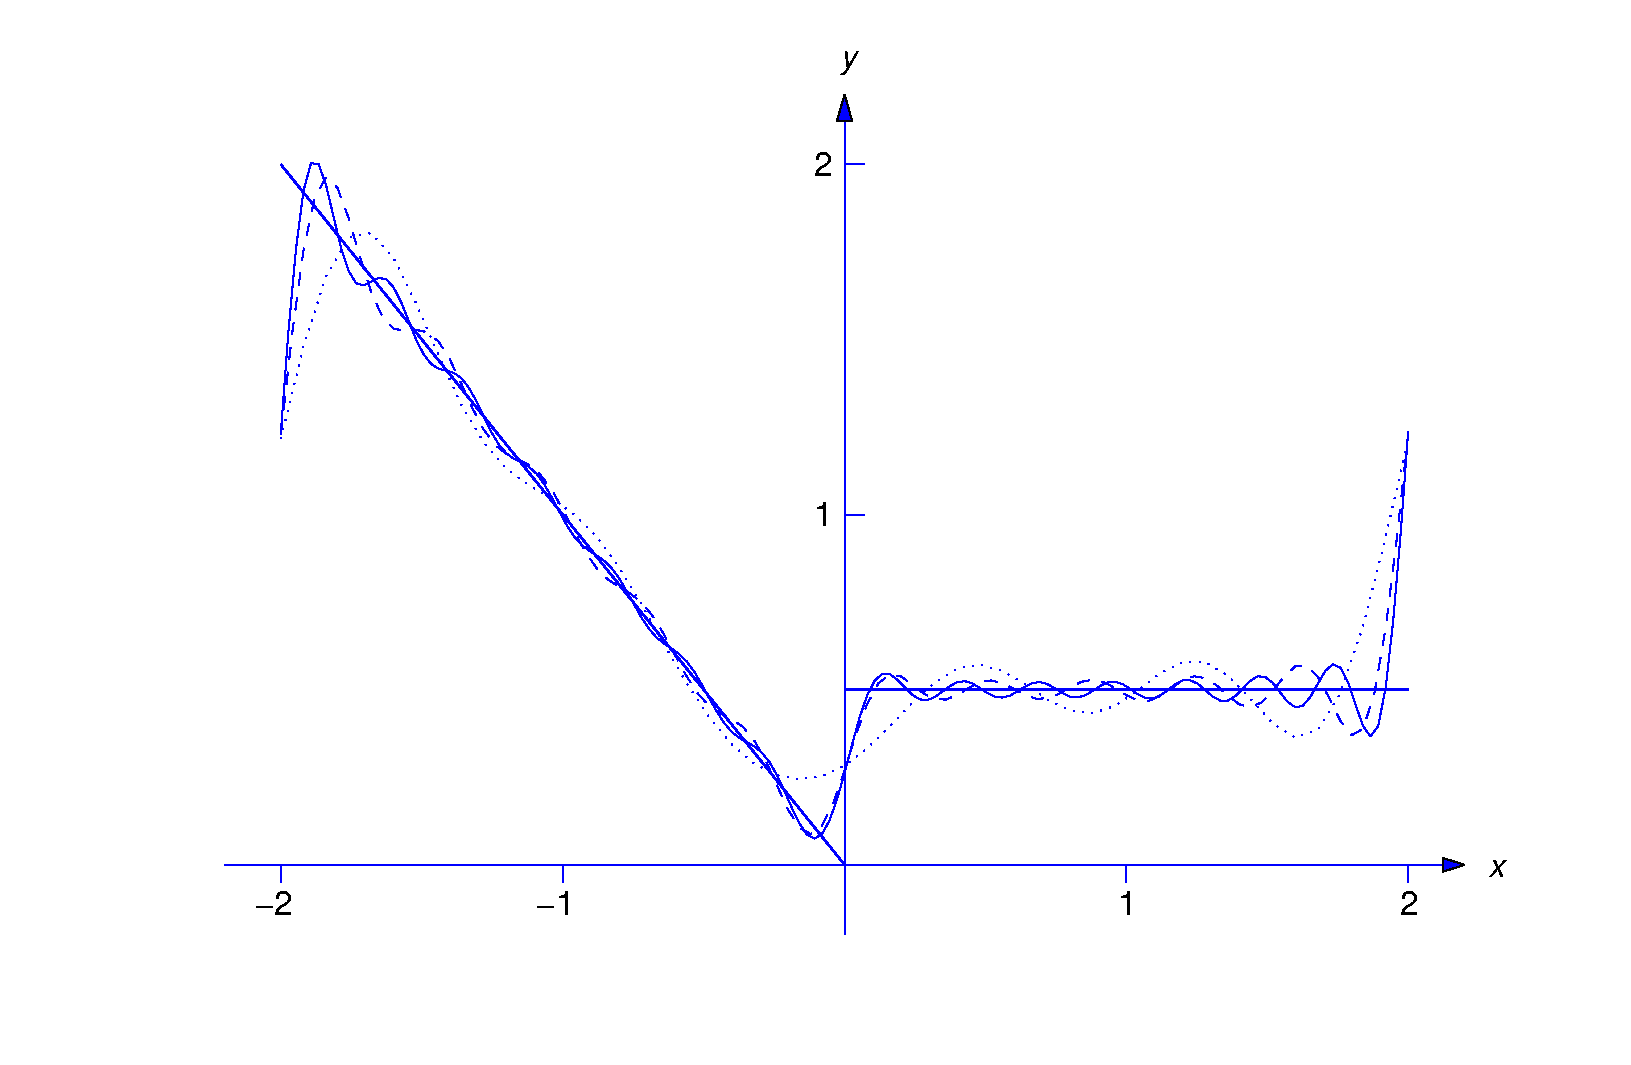
\includegraphics[bb=-78 148 689 643, width=5.67in, height=3.66in, keepaspectratio]{fig110202}
  \caption{}
  \label{figure:11.2.2}
\end{figure}
\end{examplesolution}

\setcounter{example}{1}
\begin{example}
  \label{example:11.2.2} \rm The functions $u(x)=\cos\omega x$ and $u(x)=x^{2}$ are even, while
  $v(x)=\sin\omega x$ and $v(x)=x^{3}$ are odd. The function $w(x)=e^{x}$ is neither even nor odd.
\end{example}

\setcounter{example}{2}
\begin{example}
  \label{example:11.2.3} \rm Find the Fourier series of $f(x)=x^{2}-x$ on $[-2,2]$, and determine
  its sum for $-2\le x\le2$.
\end{example}
\setcounter{equation}{8}
\setcounter{figure}{2}
\begin{examplesolution}
\solution Since $L=2$,
\[
  F(x)=a_{0}+\sum_{n=1}^{\infty}\left(a_{n}\cos\frac{n\pi x}{2}+b_{n}\sin\frac{n\pi x}{2}\right)
\]
where
\begin{equation}
  \label{eq:11.2.9}a_{0}=\frac{1}{4}\int_{-2}^{2}(x^{2}-x)\,dx,
\end{equation}
\begin{equation}
  \label{eq:11.2.10}a_{n}=\frac{1}{2}\int_{-2}^{2}(x^{2}-x)\cos\frac{n\pi x}{2}\,dx,\quad n=1,2,3,\dots,
\end{equation}
and
\begin{equation}
  \label{eq:11.2.11}b_{n}=\frac{1}{2}\int_{-2}^{2}(x^{2}-x)\sin\frac{n\pi x}{2}\,dx,\quad n=1,2,3,\dots.
\end{equation}
We simplify the evaluation of these integrals by using Theorem~11.2.5 with
$u(x)=x^{2}$ and $v(x)=x$; thus, from \eqref{eq:11.2.9},
\[
  a_{0}=\frac{1}{2}\int_{0}^{2}x^{2}\,dx=\frac{x^{3}}{6}\lims02=\frac{4}{3}.
\]
From \eqref{eq:11.2.10},
\begin{eqnarray*}
  a_{n} & = & \int_{0}^{2}x^{2}\cos\frac{n\pi x}{2}\,dx=\frac{2}{n\pi}\left[x^{2}\sin\frac{n\pi x}{2}\lims02-2\int_{0}^{2}x\sin\frac{n\pi x}{2}\,dx\right] \\
        & = & \frac{8}{n^{2}\pi^{2}}\left[x\cos\frac{n\pi x}{2}\lims02-\int_{0}^{2}\cos\frac{n\pi x}{2}\,dx\right]                                         \\
        & = & \frac{8}{n^{2}\pi^{2}}\left[2\cos n\pi-\frac{2}{n\pi}\sin\frac{n\pi x}{2}\lims02\right]=(-1)^{n}\frac{16}{n^{2}\pi^{2}}.
\end{eqnarray*}
From \eqref{eq:11.2.11},
\begin{eqnarray*}
  b_{n} & = & -\int_{0}^{2}x\sin\frac{n\pi x}{2}\,dx=\frac{2}{n\pi}\left[x\cos\frac{n\pi x}{2}\lims02-\int_{0}^{2}\cos\frac{n\pi x}{2}\,dx\right] \\
        & = & \frac{2}{n\pi}\left[2\cos n\pi-\frac{2}{n\pi}\sin\frac{n\pi x}{2}\lims02\right]=(-1)^{n}\frac{4}{n\pi}.
\end{eqnarray*}
Therefore
\[
  F(x)=\frac{4}{3}+\frac{16}{\pi^{2}}\sum_{n=1}^{\infty}\frac{(-1)^{n}}{n^{2}}\cos\frac{n\pi x}{2}+\frac{4}{\pi}\sum_{n=1}^{\infty}\frac{(-1)^{n}}{n}\sin\frac{n\pi x}{2}.
\]
Theorem~11.2.4 implies that
\[
  F(x)= \left\{
  \begin{array}{cl}
    4,       & \phantom{-}x=-2, \\
    x^{2}-x, & -2<x<2,          \\
    4,       & \phantom{-}x=2.
  \end{array}\right.
\]
Figure~\ref{figure:11.2.3} shows how the partial sum
\[
  F_{m}(x)=\frac{4}{3}+\frac{16}{\pi^{2}}\sum_{n=1}^{m}\frac{(-1)^{n}}{n^{2}}\cos\frac{n\pi x}{2}+\frac{4}{\pi}\sum_{n=1}^{m}\frac{(-1)^{n}}{n}\sin\frac{n\pi x}{2}
\]
approximates $f(x)$ for $m=5$ (dotted curve), $m=10$ (dashed curve), and $m=15$ (solid curve). \bbox

\begin{figure}[H]
  \centering
  \relax
  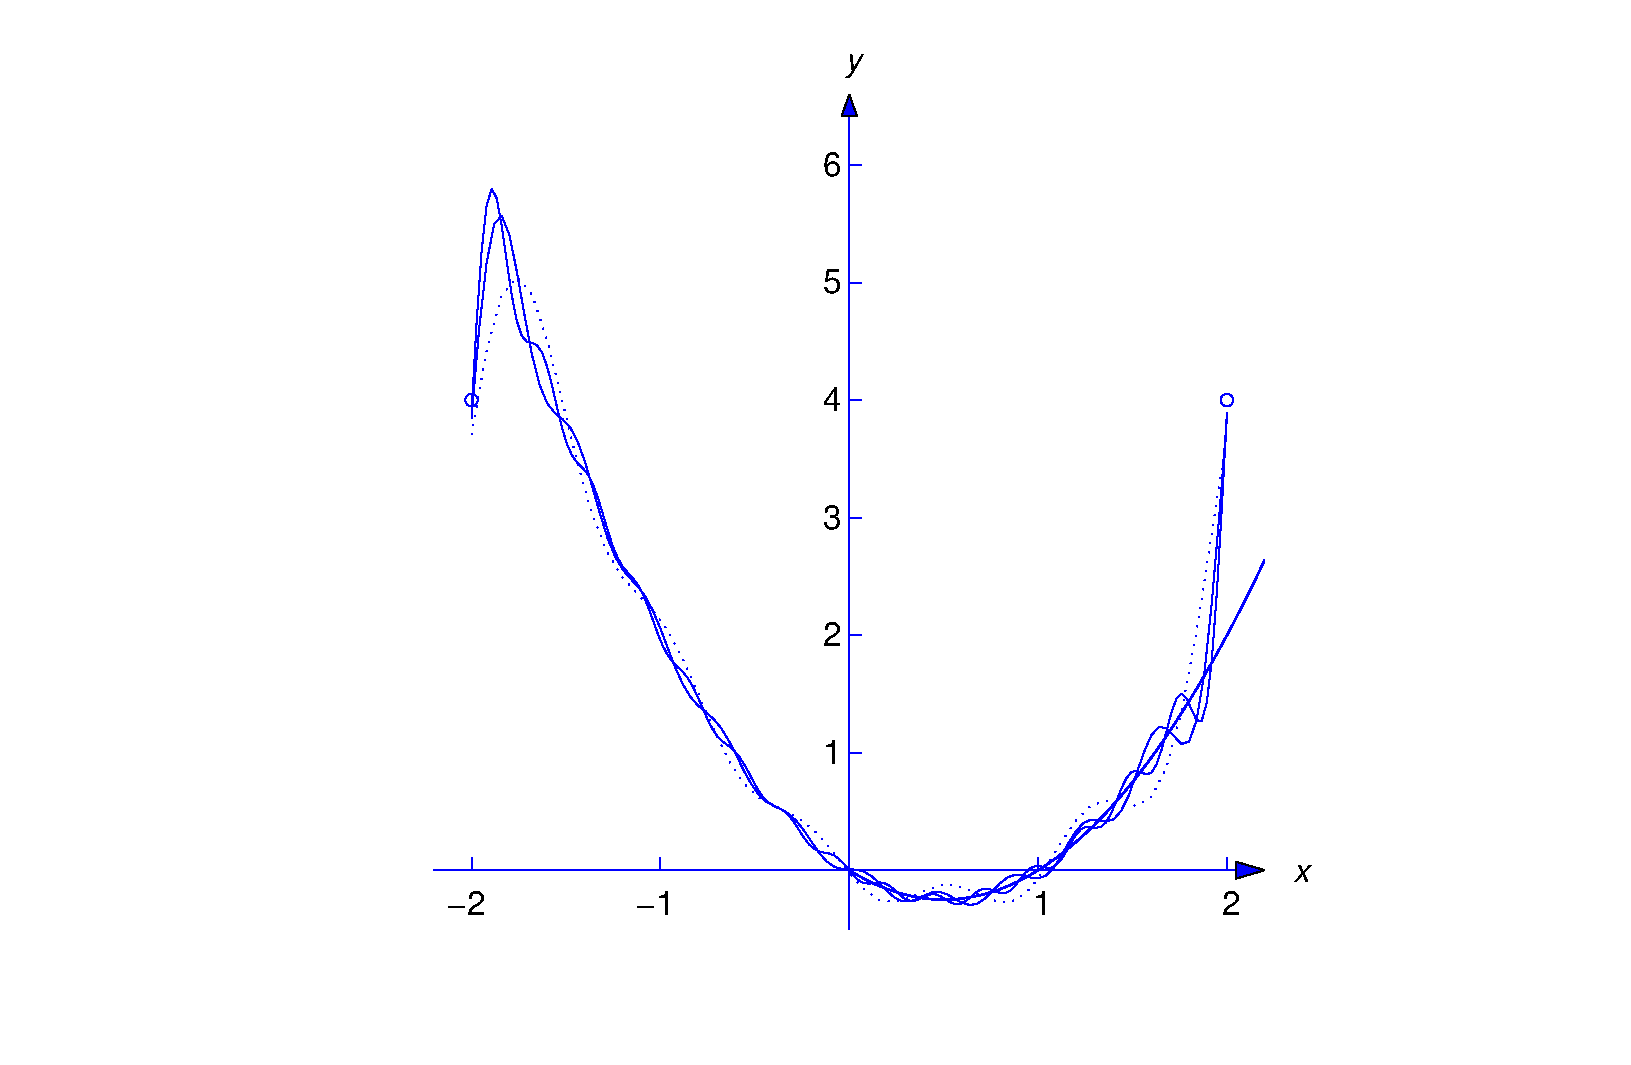
\includegraphics[bb=-78 148 689 643, width=5.67in, height=3.66in, keepaspectratio]{fig110203}
  \caption{Approximation of $f(x)=x^{2}-x$ by partial sums of its Fourier series on $[-2,2]$}
  \label{figure:11.2.3}
\end{figure}
\end{examplesolution}

\setcounter{example}{3}
\begin{example}
  \label{example:11.2.4} \rm Find the Fourier series of $f(x)=x$ on $[-\pi,\pi]$, and determine its
  sum for $-\pi\le x\le\pi$.
\end{example}
\setcounter{figure}{3}
\begin{examplesolution}
\solution Since $f$ is odd and $L=\pi$,
\[
  F(x)=\sum_{n=1}^{\infty}b_{n}\sin nx
\]
where
\begin{eqnarray*}
  b_{n} & = & \frac{2}{\pi}\int_{0}^{\pi}x\sin nx\,dx=-\frac{2}{n\pi}\left[x\cos nx\lims0\pi-\int_{0}^{\pi}\cos nx\,dx\right] \\
        & = & -\frac{2}{n}\cos n\pi+\frac{2}{n^{2}\pi}\sin nx\lims0\pi=(-1)^{n+1}\frac{2}{n}.
\end{eqnarray*}
Therefore
\[
  F(x)=-2\sum_{n=1}^{\infty}\frac{(-1)^{n}}{n}\sin nx.
\]
Theorem~11.2.4 implies that
\[
  F(x)= \left\{
  \begin{array}{cl}
    0, & \phantom{-}x=-\pi, \\
    x, & -\pi<x<\pi,        \\
    0, & \phantom{-}x=\pi.
  \end{array}\right.
\]
Figure~\ref{figure:11.2.4} shows how the partial sum
\[
  F_{m}(x)=-2\sum_{n=1}^{m}\frac{(-1)^{n}}{n}\sin nx
\]
approximates $f(x)$ for $m=5$ (dotted curve), $m=10$ (dashed curve), and $m=15$ (solid curve).

\begin{figure}[H]
  \centering
  \relax
  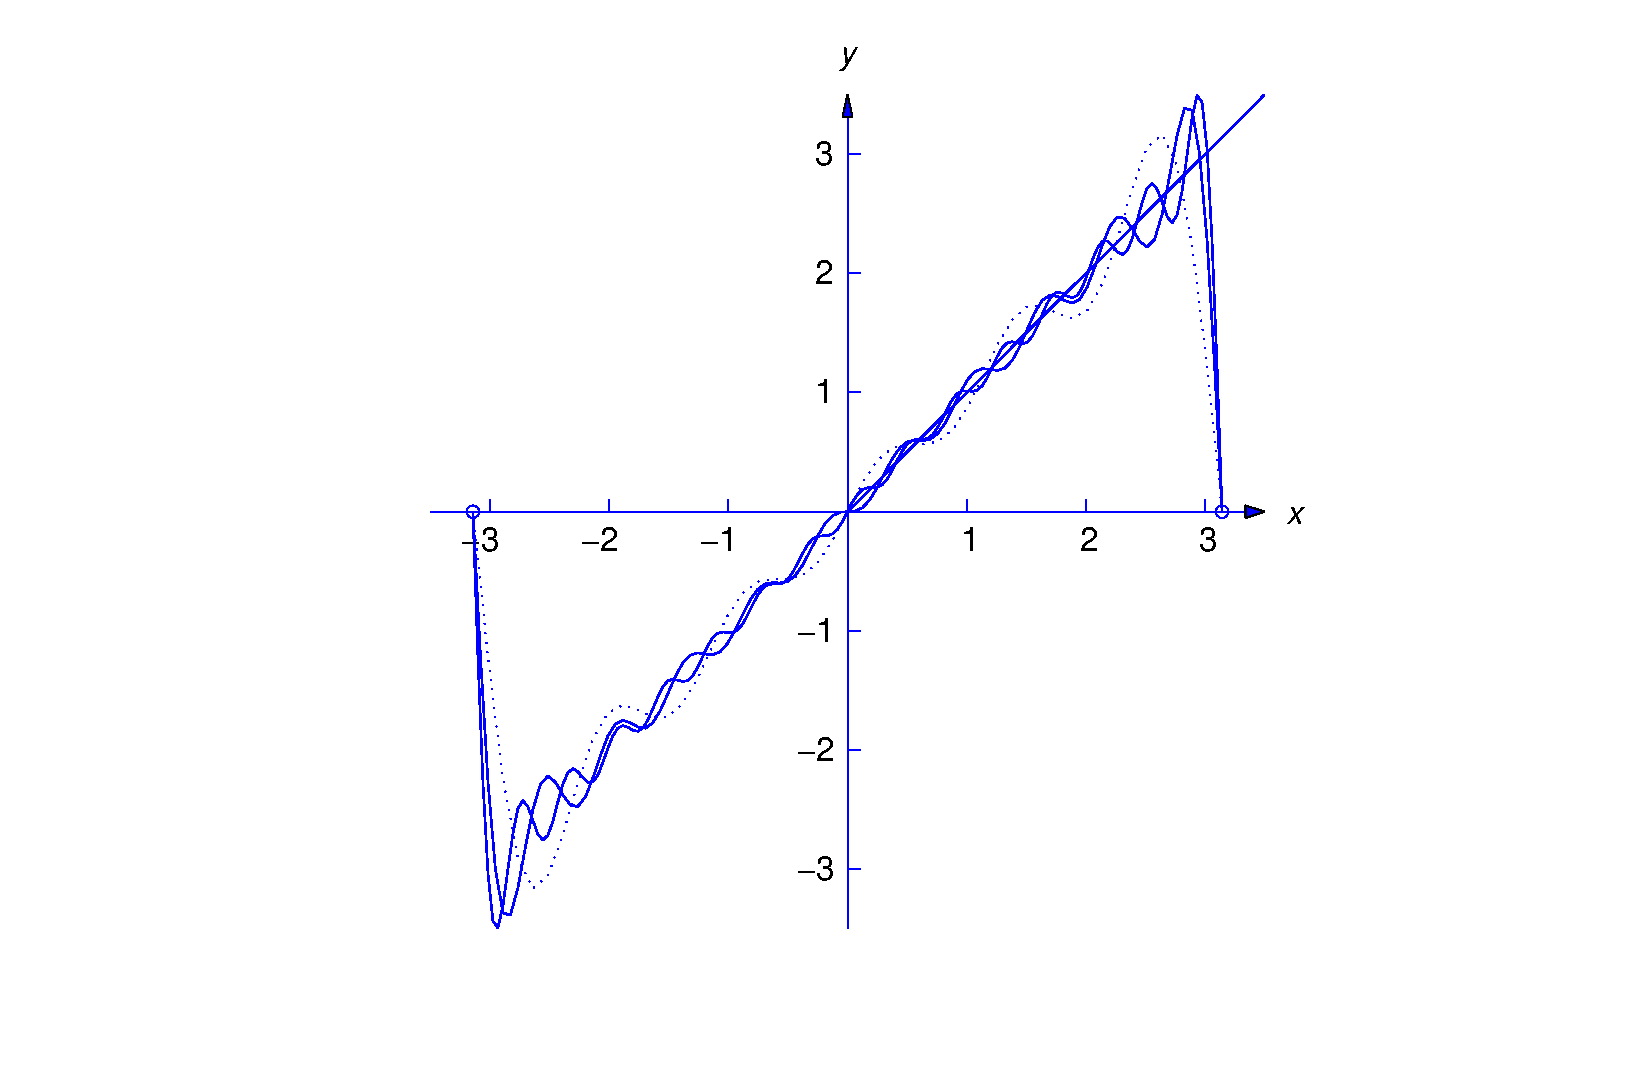
\includegraphics[bb=-78 148 689 643, width=5.67in, height=3.66in, keepaspectratio]{fig110204}
  \caption{Approximation of $f(x)=x$ by partial sums of its Fourier series on $[-\pi,\pi]$}
  \label{figure:11.2.4}
\end{figure}
\end{examplesolution}

\setcounter{example}{4}
\begin{example}
  \label{example:11.2.5} \rm Find the Fourier series of $f(x)=|x|$ on $[-\pi,\pi]$ and determine its sum for\\ $-\pi\le x\le\pi$.
\end{example}
\setcounter{equation}{11}
\begin{examplesolution}
\solution Since $f$ is even and $L=\pi$,
\[
  F(x)=a_{0}+\sum_{n=1}^{\infty}a_{n}\cos nx.
\]
Since $f(x)=x$ if $x\ge0$,
\[
  a_{0}=\frac{1}{\pi}\int_{0}^{\pi}x\,dx=\frac{x^{2}}{2\pi}\lims0\pi=\frac{\pi}{2}
\]
and, if $n\ge1$,
\begin{eqnarray*}
  a_{n} & = & \frac{2}{\pi}\int_{0}^{\pi}x\cos nx\,dx=\frac{2}{n\pi}\left[x\sin nx\lims0\pi-\int_{0}^{\pi}\sin nx\,dx\right] \\
        & = & \frac{2}{n^{2}\pi}\cos nx\lims0\pi=\frac{2}{n^{2}\pi}(\cos n\pi-1)=\frac{2}{n^{2}\pi}[(-1)^{n}-1].
\end{eqnarray*}
Therefore
\begin{equation}
  \label{eq:11.2.12}F(x)=\frac{\pi}{2}+\frac{2}{\pi}\sum_{n=1}^{\infty}\frac{(-1)^{n}-1}{n^{2}}\cos nx.
\end{equation}
However, since
\[
  (-1)^{n}-1= \left\{
  \begin{array}{rl}
    0  & \mbox{ if }n=2m,   \\
    -2 & \mbox{ if }n=2m+1,
  \end{array}\right.
\]
the terms in \eqref{eq:11.2.12} for which $n=2m$ are all zeros. Therefore we only need to include the
terms for which $n=2m+1$; that is, we can rewrite \eqref{eq:11.2.12} as
\[
  F(x)=\frac{\pi}{2}-\frac{4}{\pi}\sum_{m=0}^{\infty}\frac{1}{(2m+1)^{2}}\cos(2m+1)x.
\]
However, since the name of the index of summation doesn't matter, we prefer to replace $m$ by $n$,
and write
\[
  F(x)=\frac{\pi}{2}-\frac{4}{\pi}\sum_{n=0}^{\infty}\frac{1}{(2n+1)^{2}}\cos(2n+1)x.
\]
Since $|x|$ is continuous for all $x$ and $|-\pi|=|\pi|$, Theorem~11.2.4 implies that
$F(x)=|x|$ for all $x$ in $[-\pi,\pi]$.
\end{examplesolution}

\setcounter{example}{5}
\begin{example}
  \label{example:11.2.6} \rm Find the Fourier series of $f(x)=x(x^{2}-L^{2})$ on $[-L,L]$, and
  determine its sum for $-L\le x\le L$.
\end{example}
\begin{examplesolution}
\solution Since $f$ is odd,
\[
  F(x)=\sum_{n=1}^{\infty}b_{n}\sin\frac{n\pi x}{L},
\]
where
\begin{eqnarray*}
  b_{n} & = & \frac{2}{L}\int_{0}^{L}x(x^{2}-L^{2})\sin\frac{n\pi x}{L}\,dx                                                            \\
        & = & -\frac{2}{n\pi}\left[x(x^{2}-L^{2})\cos\frac{n\pi x}{L}\lims0L-\int_{0}^{L}(3x^{2}-L^{2})\cos\frac{n\pi x}{L}\,dx\right] \\
        & = & \frac{2L}{n^{2}\pi^{2}}\left[(3x^{2}-L^{2})\sin\frac{n\pi x}{L}\lims0L-6\int_{0}^{L}x\sin\frac{n\pi x}{L}\,dx\right]     \\
        & = & \frac{12L^{2}}{n^{3}\pi^{3}}\left[x\cos\frac{n\pi x}{L}\lims0L-\int_{0}^{L}\cos\frac{n\pi x}{L}\,dx\right]=(-1)^{n}\frac{12L^{3}}{n^{3}\pi^{3}}.
\end{eqnarray*}
Therefore
\[
  F(x)=\frac{12L^{3}}{\pi^{3}}\sum_{n=1}^{\infty}\frac{(-1)^{n}}{n^{3}}\sin\frac{n\pi x}{L}.
\]
Theorem~11.2.4 implies that $F(x)=x(x^{2}-L^{2})$ for all $x$ in $[-L,L]$.
\end{examplesolution}

\setcounter{example}{6}
\begin{example}[Gibbs Phenomenon]
  \label{example:11.2.7}\rm The Fourier series of
  \[
    f(x)=\left\{
    \begin{array}{cl}
      0, & -1<x<-\frac{1}{2},           \\
      1, & -\frac{1}{2}<x<\frac{1}{2},  \\[2\jot]
      0, & \phantom{-}{\frac{1}{2}}<x<1
    \end{array}\right.
  \]
  on $[-1,1]$ is
  \[
    F(x)=\frac{1}{2}+\frac{2}{\pi}\sum_{n=1}^{\infty}\frac{(-1)^{n-1}}{2n-1}\cos(2n-1)\pi x.
  \]
  (Verify.) According to Theorem~11.2.4,
  \[
    F(x)=\left\{
    \begin{array}{cl}
      0,           & -1\le x<-\frac{1}{2},       \\
      \frac{1}{2}, & x=-\frac{1}{2},             \\
      1,           & -\frac{1}{2}<x<\frac{1}{2}, \\
      \frac{1}{2}, & x=\frac{1}{2},              \\
      0,           & \frac{1}{2}<x\le1;
    \end{array}\right.
  \]
  thus, $F$ (as well as $f$) has unit jump discontinuities at $x=\pm\frac{1}{2}$.
  Figures~\ref{figure:11.2.5}-\ref{figure:11.2.7} show the graphs of $y=f(x)$ and
  \[
    y=F_{2N-1}(x)=\frac{1}{2}+ \frac{2}{\pi}\sum_{n=1}^{N}\frac{(-1)^{n-1}}{2n-1}\cos(2n-1)\pi x
  \]
  for $N=10$, $20$, and $30$. You can see that although $F_{2N-1}$ approximates $F$ (and therefore
  $f$) well on larger intervals as $N$ increases, the maximum absolute values of the errors remain
  approximately equal to $.09$, but occur closer to the discontinuities $x=\pm\frac{1}{2}$ as $N$
  increases.
\end{example}
\setcounter{figure}{4}
\begin{examplesolution}
\begin{figure}[H]
  \relax
  \begin{minipage}[b]{0.5\linewidth}
    \centering
    \scalebox{.65}{
    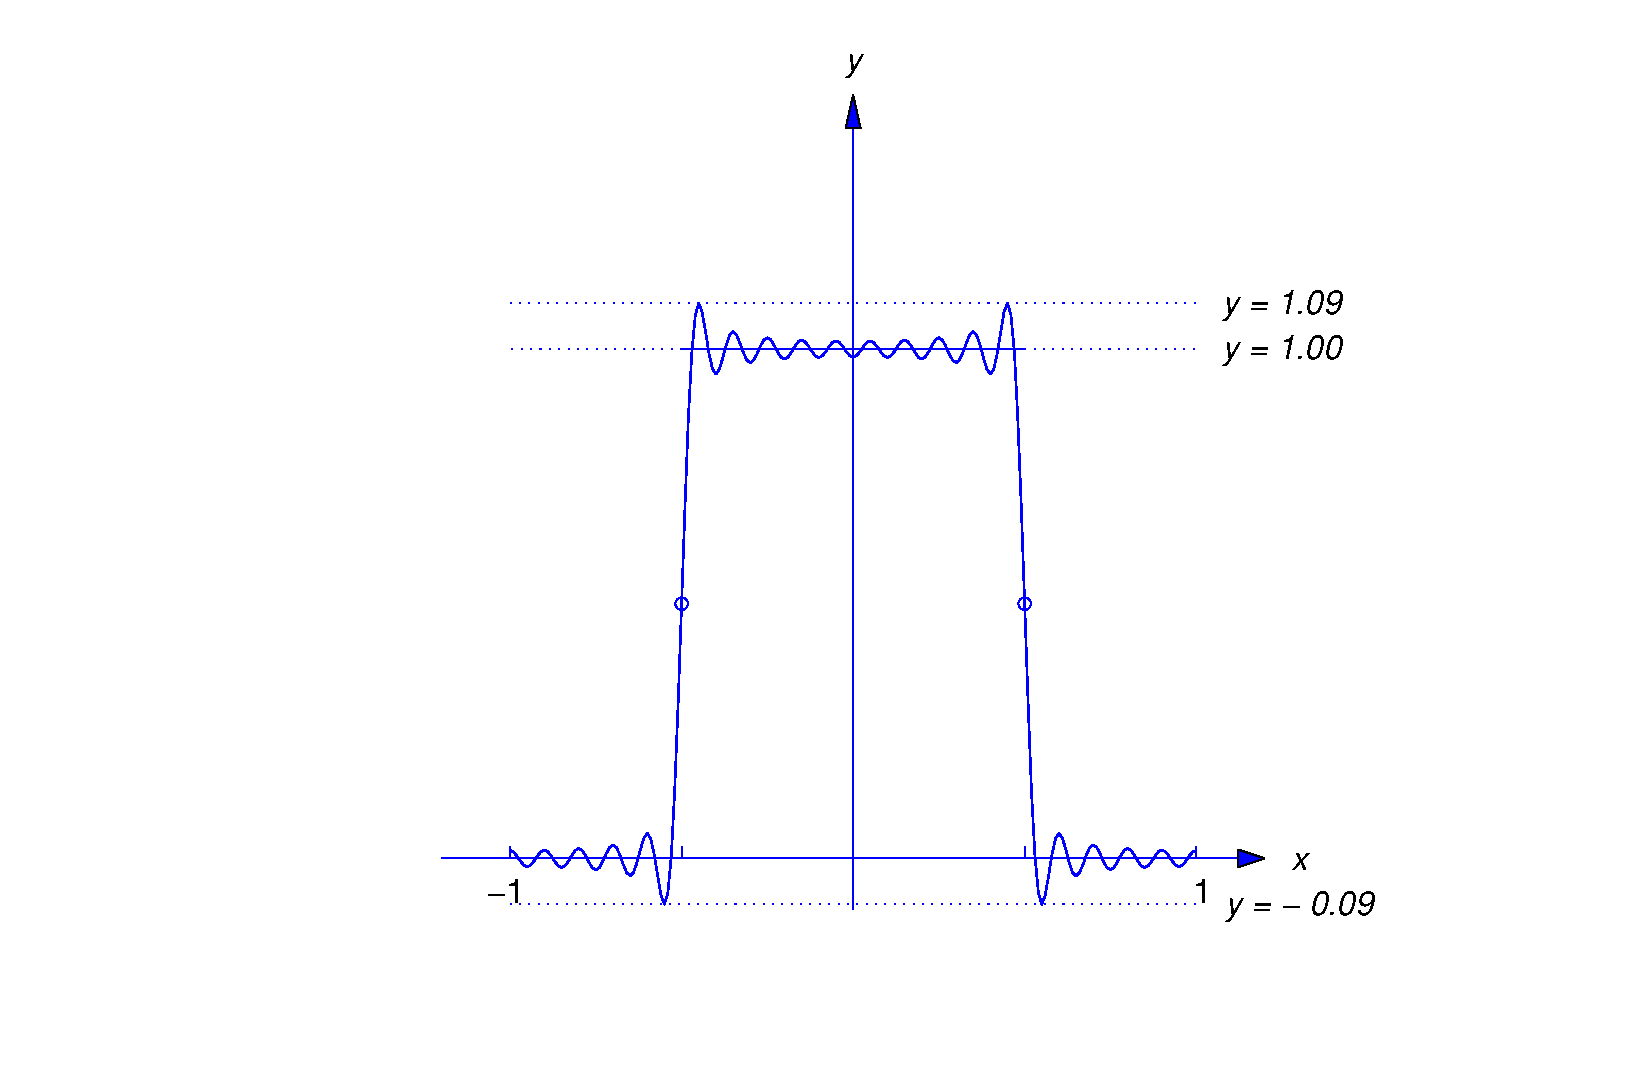
\includegraphics[bb=-78 148 689 643, width=5.67in, height=3.66in, keepaspectratio]{fig110205}}
    \caption{The Gibbs Phenomenon: Example~\ref{example:11.2.7}, $N=10$}
    \label{figure:11.2.5}
  \end{minipage}
  \begin{minipage}[b]{0.5\linewidth}
    \centering
    \scalebox{.65}{
    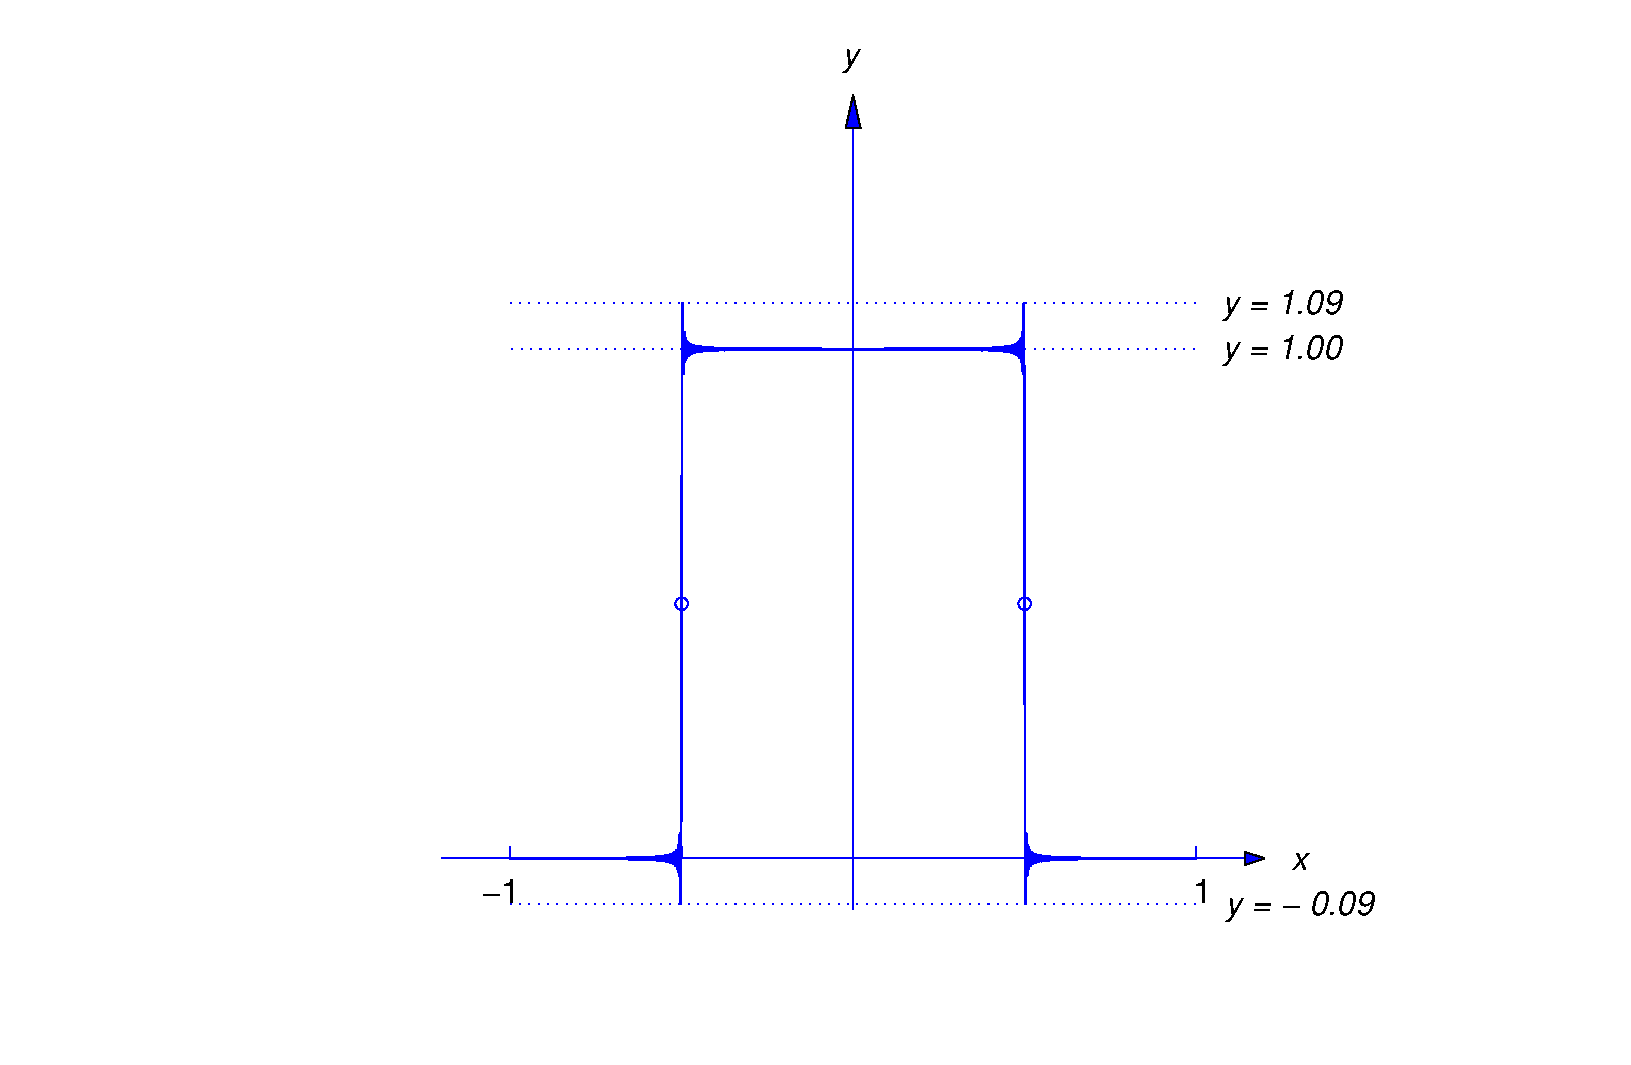
\includegraphics[bb=-78 148 689 643, width=5.67in, height=3.66in, keepaspectratio]{fig110206}}
    \caption{The Gibbs Phenomenon: Example~\ref{example:11.2.7}, $N=20$}
    \label{figure:11.2.6}
  \end{minipage}
\end{figure}

\newpage

\begin{figure}[H]
  \centering
  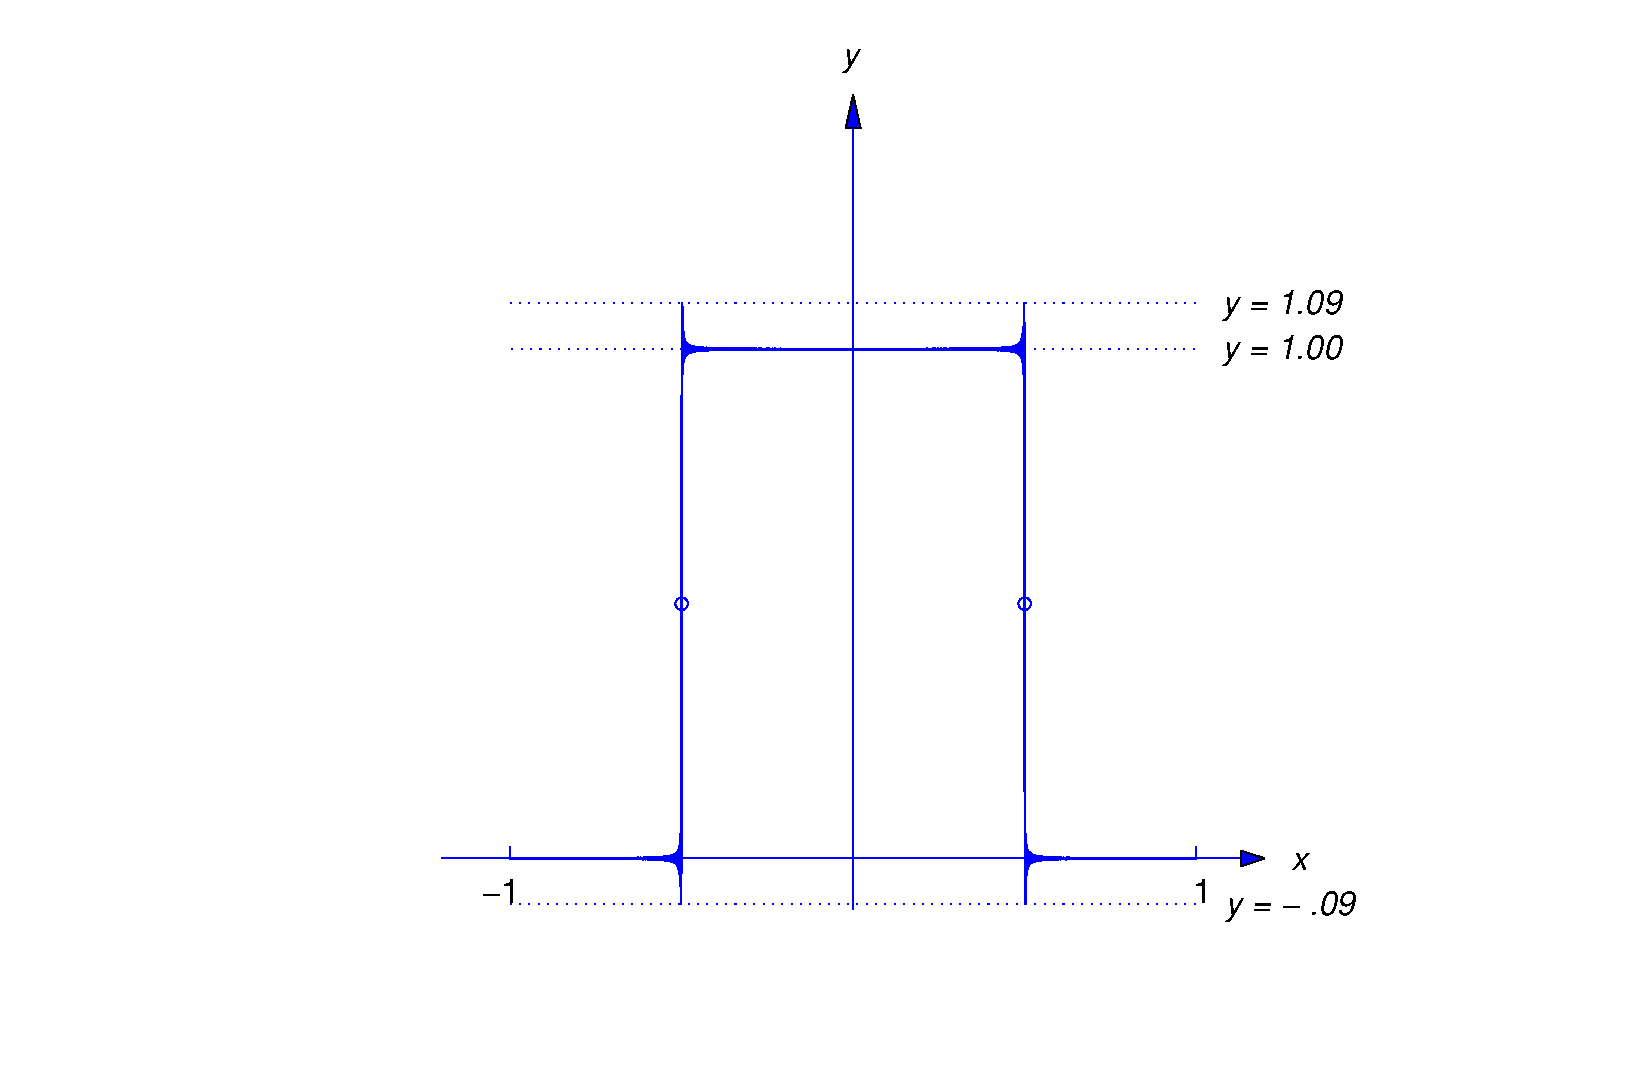
\includegraphics[bb=-78 148 689 643, width=5.67in, height=3.66in, keepaspectratio]{fig110207}
  \caption{The Gibbs Phenomenon: Example~\ref{example:11.2.7}, $N=30$}
  \label{figure:11.2.7}
\end{figure}
\end{examplesolution}

\section*{Section 11.3}
\setcounter{chapter}{11}
\setcounter{section}{3}

\setcounter{example}{0}
\begin{example}
  \label{example:11.3.1} \rm Find the Fourier cosine series of $f(x)=x$ on $[0,L]$.
\end{example}
\begin{examplesolution}
\solution The coefficients are
\[
  a_{0}=\frac{1}{L}\int_{0}^{L}x\,dx=\frac{1}{L}\frac{x^{2}}{2}\lims0L=\frac{L}{2}
\]
and, if $n\ge1$
\begin{eqnarray*}
  a_{n}&=&\frac{2}{L}\int_{0}^{L}x\cos\frac{n\pi x}{L}\,dx =\frac{2}{n\pi}\left[x\sin\frac{n\pi x}{L}\lims0L- \int_{0}^{L} \sin\frac{n\pi x}{L}\,dx\right]\\ &=&-\frac{2}{n\pi}\int_{0}^{L} \sin\frac{n\pi x}{L}\,dx =\frac{2L}{n^{2}\pi^{2}}\cos\frac{n\pi x}{L}\lims0L =\frac{2L}{n^{2}\pi^{2}}[(-1)^{n}-1]\\ &=& \left\{
  \begin{array}{cl}
    \dst-\frac{4L}{(2m-1)^{2}\pi^{2}} & \mbox{if $n=2m-1$}, \\
    0                                 & \mbox{if $n=2m$}.
  \end{array}\right.
\end{eqnarray*}
Therefore
\[
  C(x)=\dst\frac{L}{2}-\frac{4L}{\pi^{2}}\sum_{n=1}^{\infty}\frac{1}{(2n-1)^{2}}\cos\frac{(2n-1)\pi x}{L}.
\]
Theorem~11.3.1 implies that
\[
  C(x)=x,\quad0\le x\le L.
\]
\end{examplesolution}

\setcounter{example}{1}
\begin{example}
  \label{example:11.3.2} \rm Find the Fourier sine series of $f(x)=x$ on $[0,L]$.
\end{example}
\begin{examplesolution}
\solution The coefficients are
\begin{eqnarray*}
  b_{n} & = & \frac{2}{L}\int_{0}^{L}x\sin\frac{n\pi x}{L}\,dx=-\frac{2}{n\pi}\left[x\cos\frac{n\pi x}{L}\lims0L-\int_{0}^{L}\cos\frac{n\pi x}{L}\,dx\right] \\
        & = & (-1)^{n+1}\frac{2L}{n\pi}+\frac{2L}{n^{2}\pi^{2}}\sin\frac{n\pi x}{L}\lims0L=(-1)^{n+1}\frac{2L}{n\pi}.
\end{eqnarray*}
Therefore
\[
  S(x)=\dst-\frac{2L}{\pi}\sum_{n=1}^{\infty}\frac{(-1)^{n}}{n}\sin\frac{n\pi x}{L}.
\]
Theorem~11.3.2 implies that
\[
  S(x)= \left\{
  \begin{array}{cl}
    x, & 0\le x<L, \\
    0, & x=L.
  \end{array}\right.
\]
\end{examplesolution}

\setcounter{example}{2}
\begin{example}
  \label{example:11.3.3} \rm Find the mixed Fourier cosine series of $f(x)=x-L$ on $[0,L]$.
\end{example}
\begin{examplesolution}
\solution The coefficients are
\begin{eqnarray*}
  c_{n} & = & \frac{2}{L}\int_{0}^{L}(x-L)\cos\frac{(2n-1)\pi x}{2L}\,dx                                                        \\
        & = & \frac{4}{(2n-1)\pi}\left[(x-L)\sin\frac{(2n-1)\pi x}{2L}\lims0L-\int_{0}^{L}\sin\frac{(2n-1)\pi x}{2L}\,dx\right] \\
        & = & \frac{8L}{(2n-1)^{2}\pi^{2}}\cos\frac{(2n-1)\pi x}{2L}\lims0L=-\frac{8L}{(2n-1)^{2}\pi^{2}}.
\end{eqnarray*}
Therefore
\[
  C_{M}(x)=-\frac{8L}{\pi^{2}}\sum_{n=1}^{\infty}\frac{1}{(2n-1)^{2}}\cos\frac{(2n-1)\pi x}{2L}.
\]
Theorem~11.3.3 implies that
\[
  C_{M}(x)=x-L,\quad0\le x\le L.
\]
\end{examplesolution}

\setcounter{example}{3}
\begin{example}
  \label{example:11.3.4} \rm Find the mixed Fourier sine series of $f(x)=x$ on $[0,L]$.
\end{example}
\begin{examplesolution}
\solution The coefficients are
\begin{eqnarray*}
  d_{n} & = & \frac{2}{L}\int_{0}^{L}x\sin\frac{(2n-1)\pi x}{2L}\,dx                                                         \\
        & = & -\frac{4}{(2n-1)\pi}\left[x\cos\frac{(2n-1)\pi x}{2L}\lims0L-\int_{0}^{L}\cos\frac{(2n-1)\pi x}{2L}\,dx\right] \\
        & = & \frac{4}{(2n-1)\pi}\int_{0}^{L}\cos\frac{(2n-1)\pi x}{2L}\,dx                                                  \\
        & = & \frac{8L}{(2n-1)^{2}\pi^{2}}\sin\frac{(2n-1)\pi x}{2L}\lims0L=(-1)^{n+1}\frac{8L}{(2n-1)^{2}\pi^{2}}.
\end{eqnarray*}
Therefore
\[
  S_{M}(x)=-\frac{8L}{\pi^{2}}\sum_{n=1}^{\infty}\frac{(-1)^{n}}{(2n-1)^{2}}\sin\frac{(2n-1)\pi x}{2L}.
\]
Theorem~11.3.4 implies that
\[
  S_{M}(x)=x,\quad0\le x\le L.
\]
\end{examplesolution}

\setcounter{example}{4}
\begin{example}
  \label{example:11.3.5} \rm Find the Fourier cosine expansion of $f(x)=x^{2}(3L-2x)$ on $[0,L]$.
\end{example}
\begin{examplesolution}
\solution Here
\[
  a_{0}=\frac{1}{L}\int_{0}^{L}(3Lx^{2}-2x^{3})\,dx=\frac{1}{L}\left(Lx^{3}-\frac{x^{4}}{2}\right)\lims0L=\frac{L^{3}}{2}
\]
and
\[
  a_{n}=\frac{2}{L}\int_{0}^{L}(3Lx^{2}-2x^{3})\cos\frac{n\pi x}{L}\,dx,\quad n\ge1.
\]
Evaluating this integral directly is laborious. However, since $f'(x)=6Lx-6x^{2}$, we see that
$f'(0)=f'(L)=0$. Since $f'''(x)=-12$, we see from (11.3.4) that if $n\ge1$ then
\begin{eqnarray*}
  a_{n}&=&-\frac{24L^{2}}{n^{3}\pi^{3}}\int_{0}^{L}\sin\frac{n\pi x}{L}\,dx =\frac{24L^{3}}{n^{4}\pi^{4}}\cos\frac{n\pi x}{L}\lims0L=\frac{24L^{3}}{n^{4}\pi^{4}}[(-1)^{n}-1]\\ &=& \left\{
  \begin{array}{cl}
    \dst-\frac{48L^{3}}{(2m-1)^{4}\pi^{4}} & \mbox{if $n=2m-1$}, \\
    0                                      & \mbox{if $n=2m$.}
  \end{array}\right.
\end{eqnarray*}
Therefore
\[
  C(x)=\frac{L^{3}}{2}-\frac{48L^{3}}{\pi^{4}}\sum_{n=1}^{\infty}\frac{1}{(2n-1)^{4}}\cos\frac{(2n-1)\pi x}{L}.
\]
\end{examplesolution}

\setcounter{example}{5}
\begin{example}
  \label{example:11.3.6} \rm Find the Fourier sine expansion of $f(x)=x(x^{2}-3Lx+2L^{2})$ on
  $[0,L]$.
\end{example}
\begin{examplesolution}
\solution Since $f(0)=f(L)=0$ and $f''(x)=6(x-L)$, we see from (11.3.5) that
\begin{eqnarray*}
  b_{n} & = & -\frac{12L}{n^{2}\pi^{2}}\int_{0}^{L}(x-L)\sin\frac{n\pi x}{L}\,dx                                             \\
        & = & \frac{12L^{2}}{n^{3}\pi^{3}}\left[(x-L)\cos\frac{n\pi x}{L}\lims0L-\int_{0}^{L}\cos\frac{n\pi x}{L}\,dx\right] \\
        & = & \frac{12L^{2}}{n^{3}\pi^{3}}\left[L-\frac{L}{n\pi}\sin\frac{n\pi x}{L}\lims0L\right]=\frac{12L^{3}}{n^{3}\pi^{3}}.
\end{eqnarray*}
Therefore
\[
  S(x)=\dst\frac{12L^{3}}{\pi^{3}}\sum_{n=1}^{\infty}\frac{1}{n^{3}}\sin\frac{n\pi x}{L}.
\]
\end{examplesolution}

\setcounter{example}{6}
\begin{example}
  \label{example:11.3.7} \rm Find the mixed Fourier cosine expansion of $f(x)=3x^{3}-4Lx^{2}+L^{3}$
  on $[0,L]$.
\end{example}
\begin{examplesolution}
\solution Since $f'(0)=f(L)=0$ and $f''(x)=2(9x-4L)$, we see from (11.3.6) that
\begin{eqnarray*}
  c_{n} & = & -\frac{16L}{(2n-1)^{2}\pi^{2}}\int_{0}^{L}(9x-4L)\cos\frac{(2n-1)\pi x}{2L}\,dx                                                     \\
        & = & -\frac{32L^{2}}{(2n-1)^{3}\pi^{3}}\left[(9x-4L)\sin\frac{(2n-1)\pi x}{2L}\lims0L-9\int_{0}^{L}\sin\frac{(2n-1)\pi x}{2L}\,dx\right] \\
        & = & -\frac{32L^{2}}{(2n-1)^{3}\pi^{3}}\left[(-1)^{n+1}5L+\frac{18L}{(2n-1)\pi}\cos\frac{(2n-1)\pi x}{2L}\lims0L\right]                  \\
        & = & \frac{32L^{3}}{(2n-1)^{3}\pi^{3}}\left[(-1)^{n}5+\frac{18}{(2n-1)\pi}\right].
\end{eqnarray*}
Therefore
\[
  C_{M}(x)=\dst\frac{32L^{3}}{\pi^{3}}\sum_{n=1}^{\infty}\frac{1}{(2n-1)^{3}}\left[ (-1)^{n}5+\frac{18}{(2n-1)\pi}\right]\cos\frac{(2n-1)\pi x}{2L}.
\]
\end{examplesolution}

\setcounter{example}{7}
\begin{example}
  \label{example:11.3.8} \rm Find the mixed Fourier sine expansion of
  \[
    f(x)=x(2x^{2}-9Lx+12L^{2})
  \]
  on $[0,L]$.
\end{example}
\begin{examplesolution}
\solution Since $f(0)=f'(L)=0$, and $f''(x)=6(2x-3L)$, we see from (11.3.7) that
\begin{eqnarray*}
  d_{n} & = & -\dst\frac{48L}{(2n-1)^{2}\pi^{2}}\int_{0}^{L}(2x-3L)\sin\frac{(2n-1)\pi x}{2L}\,dx                                                    \\
        & = & \dst\frac{96L^{2}}{(2n-1)^{3}\pi^{3}}\left[(2x-3L)\cos\frac{(2n-1)\pi x}{2L}\lims0L-2\int_{0}^{L}\cos\frac{(2n-1)\pi x}{2L}\,dx\right] \\
        & = & \dst\frac{96L^{2}}{(2n-1)^{3}\pi^{3}}\left[3L-\frac{4L}{(2n-1)\pi}\sin\frac{(2n-1)\pi x}{2L}\lims0L\right]                             \\
        & = & \dst\frac{96L^{3}}{(2n-1)^{3}\pi^{3}}\left[3+(-1)^{n}\frac{4}{(2n-1)\pi}\right].
\end{eqnarray*}
Therefore
\[
  S_{M}(x) =\dst\frac{96L^{3}}{\pi^{3}}\sum_{n=1}^{\infty}\frac{1}{(2n-1)^{3}}\left[3+(-1)^{n}\frac{4}{(2n-1)\pi}\right]\sin\frac{(2n-1)\pi x}{2L}.
\]
\end{examplesolution}

\section*{Section 12.1}
\phantomsection
\addcontentsline{toc}{chapter}{Chapter 12}
\setcounter{chapter}{12}
\setcounter{section}{1}

\setcounter{example}{0}
\begin{example}
  \label{example:12.1.1} \rm Solve \textup{(12.1.4)} with $f(x)=x(x^{2}-3Lx+2L^{2})$.
\end{example}
\begin{examplesolution}
\solution From Example~\ref{example:11.3.6}, the Fourier sine series of $f$ on $[0,L]$ is
\[
  S(x)=\dst\frac{12L^{3}}{\pi^{3}}\sum_{n=1}^{\infty}\frac{1}{n^{3}}\sin\frac{n\pi x}{L}.
\]
Therefore
\[
  u(x,t)=\dst\frac{12L^{3}}{\pi^{3}}\sum_{n=1}^{\infty}\frac{1}{n^{3}}e^{-n^{2}\pi^{2}a^{2}t/L^{2}}\sin\frac{n\pi x}{L}. \eqno{\bbox}
\]
\end{examplesolution}

\setcounter{example}{1}
\begin{example}
  \label{example:12.1.2} \rm Solve \textup{(12.1.6)} with $f(x)=x$.
\end{example}
\begin{examplesolution}
\solution From Example~\ref{example:11.3.1}, the Fourier cosine series of $f$ on $[0,L]$ is
\[
  C(x)=\dst\frac{L}{2}-\frac{4L}{\pi^{2}}\sum_{n=1}^{\infty}\frac{1}{(2n-1)^{2}}\cos\frac{(2n-1)\pi x}{L}.
\]
Therefore
\[
  u(x,t)=\frac{L}{2}-\frac{4L}{\pi^{2}}\sum_{n=1}^{\infty}\frac{1}{(2n-1)^{2}}e^{-(2n-1)^{2}\pi^{2}a^{2}t/L^{2}}\cos\frac{(2n-1)\pi x}{L}. \eqno{\bbox}
\]
\end{examplesolution}

\setcounter{example}{2}
\begin{example}
  \label{example:12.1.3} \rm Solve \textup{(12.1.7)} with $f(x)=x$.
\end{example}
\setcounter{figure}{1}
\begin{examplesolution}
\solution From Example~\ref{example:11.3.4}, the mixed Fourier sine series of $f$ on $[0,L]$ is
\[
  S_{M}(x)=-\frac{8L}{\pi^{2}}\sum_{n=1}^{\infty}\frac{(-1)^{n}}{(2n-1)^{2}}\sin\frac{(2n-1)\pi x}{2L}.
\]
Therefore
\[
  u(x,t)=-\frac{8L}{\pi^{2}}\sum_{n=1}^{\infty}\frac{(-1)^{n}}{(2n-1)^{2}}e^{-(2n-1)^{2}\pi^{2}a^{2}t/4L^{2}}\sin\frac{(2n-1)\pi x}{2L}. \eqno{\bbox}
\]

Figure~\ref{figure:12.1.2} shows a graph of $u=u(x,t)$ plotted with respect to $x$ for various
values of $t$. The line $y=x$ corresponds to $t=0$. The other curves correspond to positive values
of $t$. As $t$ increases, the graphs approach the line $u=0$.

\begin{figure}[H]
  \centering
  \relax
  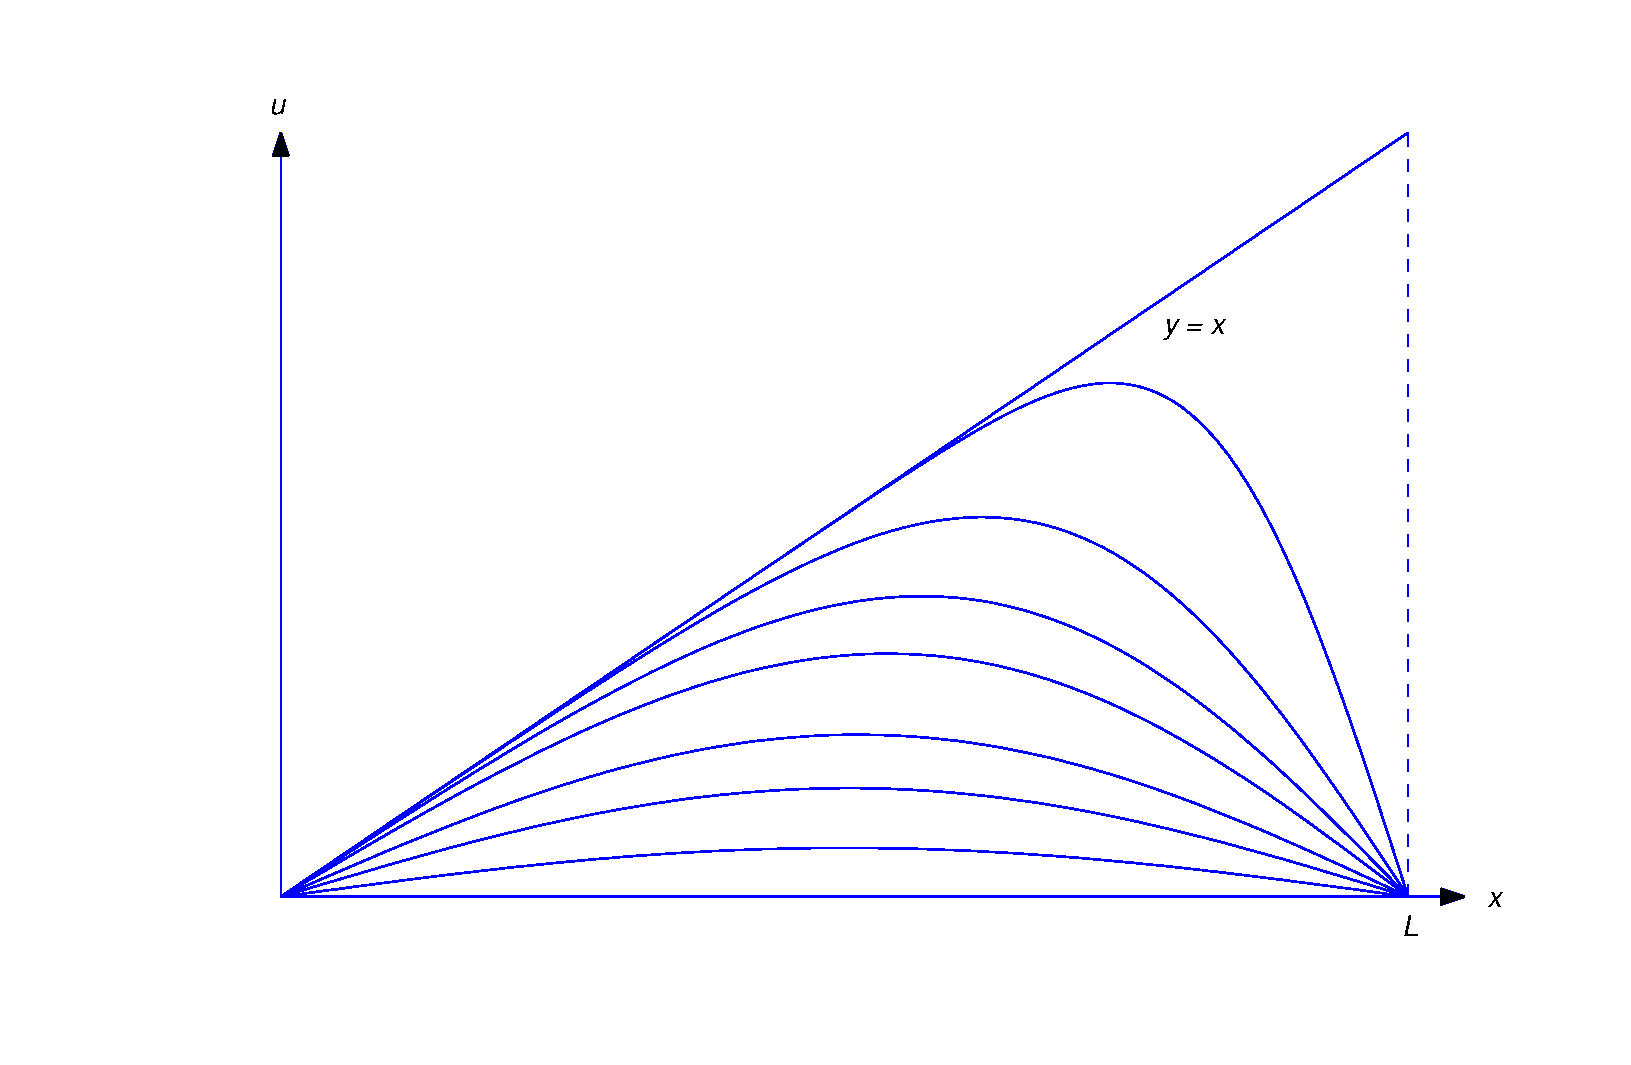
\includegraphics[bb=-78 148 689 643, width=5.67in, height=3.66in, keepaspectratio]{fig120102}
  \caption{}
  \label{figure:12.1.2}
\end{figure}
\end{examplesolution}

\setcounter{example}{3}
\begin{example}
  \label{example:12.1.4} \rm Solve \textup{(12.1.8)} with $f(x)=x-L$.
\end{example}
\begin{examplesolution}
\solution From Example~\ref{example:11.3.3}, the mixed Fourier cosine series of $f$ on $[0,L]$ is
\[
  C_{M}(x)=-\frac{8L}{\pi^{2}}\sum_{n=1}^{\infty}\frac{1}{(2n-1)^{2}}\cos\frac{(2n-1)\pi x}{2L}.
\]
Therefore
\[
  u(x,t)=-\frac{8L}{\pi^{2}}\sum_{n=1}^{\infty}\frac{1}{(2n-1)^{2}}e^{-(2n-1)^{2}\pi^{2}a^{2}t/4L^{2}}\cos\frac{(2n-1)\pi x}{2L}.
\]
\end{examplesolution}

\setcounter{example}{4}
\begin{example}
  \label{example:12.1.5} \rm Solve
  \[
    \begin{array}{c}
      u_{t}=u_{xx}-2,\quad0<x<1,\quad t>0,      \\
      u(0,t)=-1,\quad u(1,t)=1,\quad t>0,       \\
      u(x,0)=x^{3}-2x^{2}+3x-1,\quad0\le x\le1.
    \end{array}
  \]

  \solution We leave it to you to show that
  \[
    q(x)=x^{2}+x-1
  \]
  satisfies
  \[
    q''-2=0,\quad q(0)=-1,\quad q(1)=1.
  \]
  Therefore
  \[
    u(x,t)=v(x,t)+x^{2}+x-1,
  \]
  where
  \[
    v_{t}=v_{xx},\quad0<x<1,\quad t>0,
  \]
  \[
    v(0,t)=0,\quad v(1,t)=0,\quad t>0,
  \]
  and
  \[
    v(x,0)=x^{3}-2x^{2}+3x-1-x^{2}-x+1=x(x^{2}-3x+2).
  \]
  From Example~\ref{example:12.1.1} with $a=1$ and $L=1$,
  \[
    v(x,t)= \frac{12}{\pi^{3}}\sum_{n=1}^{\infty}\frac{1}{n^{3}}e^{-n^{2}\pi^{2}t}\sin n\pi x.
  \]
  Therefore
  \[
    u(x,t)=x^{2}+x-1+ \frac{12}{\pi^{3}}\sum_{n=1}^{\infty}\frac{1}{n^{3}}e^{-n^{2}\pi^{2}t}\sin n\pi x. \eqno{\bbox}
  \]
\end{example}

\section*{Section 12.2}
\setcounter{chapter}{12}
\setcounter{section}{2}

\setcounter{example}{0}
\begin{example}
  \label{example:12.2.1} \rm Solve \textup{(12.2.1)} with
  \[
    f(x)=x(x^{3}-2Lx^{2}+L^{3}) \mbox{\quad and \quad}g(x)=x(L-x).
  \]
\end{example}
\begin{examplesolution}
\solution We leave it to you to verify that $f$ and $g$ satisfy the assumptions of
Theorem~12.2.4.

From Exercise~11.3.~\hspace*{-3pt}11.3.39,
\[
  S_{f}(x)=\frac{96L^{4}}{\pi^{5}}\sum_{n=1}^{\infty}\frac{1}{(2n-1)^{5}}\sin\frac{(2n-1)\pi x}{L}.
\]
From Exercise~11.3.~\hspace*{-3pt}11.3.36,
\[
  S_{g}(x)=\frac{8L^{2}}{\pi^{3}}\sum_{n=1}^{\infty}\frac{1}{(2n-1)^{3}}\sin\frac{(2n-1)\pi x}{L}.
\]
From \textup{(12.2.8)},
\[
  \begin{array}{rcl}
    u(x,t) & = & \dst\frac{96L^{4}}{\pi^{5}}\sum_{n=1}^{\infty}\frac{1}{(2n-1)^{5}} \cos\frac{(2n-1)\pi at}{L}\sin\frac{(2n-1)\pi x}{L}    \\
           &   & + \dst\frac{8L^{3}}{a\pi^{4}}\sum_{n=1}^{\infty}\frac{1}{(2n-1)^{4}} \sin\frac{(2n-1)\pi at}{L}\sin\frac{(2n-1)\pi x}{L}.
  \end{array}
\]

Theorem~12.1.2 implies that $u_{xx}$ and $u_{tt}$ can be obtained by term by term
differentiation, for all $(x,t)$, so $u_{tt}=a^{2}u_{xx}$ for all $(x,t)$
(Exercise~12.2.62). Moreover, Theorem~11.3.2 implies that $S_{f}(x)=f(x)$
and $S_{g}(x)=g(x)$ if $0\le x\le L$. Therefore $u(x,0)=f(x)$ and $u_{t}(x,0)=g(x)$ if
$0\le x\le L$. Hence, $u$ is an actual solution of the initial-boundary value problem.
\end{examplesolution}

\section*{Section 12.3}
\setcounter{chapter}{12}
\setcounter{section}{3}

\setcounter{example}{0}
\setcounter{equation}{3}
\begin{example}
  \label{example:12.3.1} \rm Define the formal solution of
  \begin{equation}
    \label{eq:12.3.4}
    \begin{array}{c}
      u_{xx}+u_{yy}=0,\quad0<x<a,\quad0<y<b,       \\
      u(x,0)=f(x),\quad u(x,b)=0,\quad0\le x\le a, \\
      u(0,y)=0,\quad u(a,y)=0,\quad0\le y\le b
    \end{array}
  \end{equation}
  (Figure~12.3.4).
\end{example}
\setcounter{equation}{4}
\begin{examplesolution}
\solution The boundary conditions in \eqref{eq:12.3.4} require products $v(x,y)=X(x)Y(y)$ such that
$X(0)=X(a)=Y(b)=0$; hence, we let $k=-\lambda$ in \textup{(12.3.3)}. Thus, $X$ and $Y$ must satisfy
\begin{equation}
  \label{eq:12.3.5}X''+\lambda X=0,\quad X(0)=0,\quad X(a)=0
\end{equation}
and
\begin{equation}
  \label{eq:12.3.6}Y''-\lambda Y=0,\quad Y(b)=0.
\end{equation}
From Theorem~11.1.2, the eigenvalues of \eqref{eq:12.3.5} are
$\lambda_{n}=n^{2}\pi^{2}/a^{2}$, with associated eigenfunctions
\[
  X_{n}=\sin\frac{n\pi x}{a},\quad n=1,2,3,\dots.
\]
Substituting $\lambda=n^{2}\pi^{2}/a^{2}$ into \eqref{eq:12.3.6} yields
\[
  Y''-(n^{2}\pi^{2}/a^{2})Y=0,\quad Y(b)=0,
\]
so we could take
\begin{equation}
  \label{eq:12.3.7}Y_{n}=\sinh\frac{n\pi(b-y)}{a};
\end{equation}
however, because of the nonhomogeneous Dirichlet condition at $y=0$, it's better to require that
$Y_{n}(0)=1$, which can be achieved by dividing the right side of \eqref{eq:12.3.7} by its value at
$y=0$; thus, we take
\[
  Y_{n}=\frac{\sinh n\pi(b-y)/a}{\sinh n\pi b/a}.
\]
Then
\[
  v_{n}(x,y)=X_{n}(x)Y_{n}(y)=\frac{\sinh n\pi(b-y)/a}{\sinh n\pi b/a}\sin\frac{n\pi x}{a},
\]
so $v_{n}(x,0)=\sin n\pi x/a$ and $v_{n}$ satisfies \eqref{eq:12.3.4} with $f(x)=\sin n\pi x/a$.
More generally, if $\alpha_{1}$, \dots, $\alpha_{m}$ are arbitrary constants then
\[
  u_{m}(x,y)=\sum_{n=1}^{m}\alpha_{n}\frac{\sinh n\pi(b-y)/a}{\sinh n\pi b/a}\sin\frac{n\pi x}{a}
\]
satisfies \eqref{eq:12.3.4} with
\[
  f(x)=\sum_{n=1}^{m}\alpha_{n}\sin\frac{n\pi x}{a}.
\]
Therefore, if $f$ is an arbitrary piecewise smooth function on $[0,a]$, we define the formal
solution of \eqref{eq:12.3.4} to be
\begin{equation}
  \label{eq:12.3.8}u(x,y)=\sum_{n=1}^{\infty}\alpha_{n}\frac{\sinh n\pi(b-y)/a}{\sinh n\pi b/a}\sin\frac{n\pi x}{a},
\end{equation}
where
\[
  S(x)=\sum_{n=1}^{\infty}\alpha_{n}\sin\frac{n\pi x}{a}
\]
is the Fourier sine series of $f$ on $[0,a]$; that is,
\[
  \alpha_{n}=\frac{2}{a}\int_{0}^{a}f(x)\sin\frac{n\pi x}{a}\,dx,\quad n=1,2,3,\dots. \eqno{\bbox}
\]

If $y<b$ then
\begin{equation}
  \label{eq:12.3.9}\frac{\sinh n\pi(b-y)/a}{\sinh n\pi b/a}\approx e^{-n\pi y/a}
\end{equation}
for large $n$, so the series in \eqref{eq:12.3.8} converges if $0<y<b$; moreover, since also
\[
  \frac{\cosh n\pi(b-y)/a}{\sinh n\pi b/a}\approx e^{-n\pi y/a}
\]
for large $n$, Theorem~12.1.2 applied twice with $z=x$ and twice with $z=y$ shows
that $u_{xx}$ and $u_{yy}$ can be obtained by differentiating $u$ term by term if $0<y<b$.
(Exercise~12.3.37). Therefore $u$ satisfies Laplace's equation in the interior of the
rectangle in Figure~12.3.4. Moreover, the series in \eqref{eq:12.3.8} also converges on
the boundary of the rectangle, and satisfies the three homogeneous boundary conditions in
\eqref{eq:12.3.4}. Therefore, since $u(x,0)=S(x)$ for $0\le x\le a$, $u$ is an actual solution of
\eqref{eq:12.3.4} if and only if $S(x)=f(x)$ for $0\le x\le a$. From Theorem~11.3.2,
this is true if $f$ is continuous and piecewise smooth on $[0,a]$, and $f(0)=f(a)=0$.
\end{examplesolution}

\setcounter{example}{1}
\begin{example}
  \label{example:12.3.2} \rm Solve \eqref{eq:12.3.4} with $f(x)=x(x^{2}-3ax+2a^{2})$.
\end{example}
\setcounter{equation}{9}
\setcounter{figure}{4}
\begin{examplesolution}
\solution From Example~\ref{example:11.3.6},
\[
  S(x)=\frac{12a^{3}}{\pi^{3}}\sum_{n=1}^{\infty}\frac{1}{n^{3}}\sin\frac{n\pi x}{a}.
\]
Therefore
\begin{equation}
  \label{eq:12.3.10}u(x,y)=\frac{12a^{3}}{\pi^{3}}\sum_{n=1}^{\infty}\frac{\sinh n\pi(b-y)/a}{n^{3}\sinh n\pi b/a}\sin\frac{n\pi x}{a}.
\end{equation}

To compute approximate values of $u(x,y)$, we must use partial sums of the form
\[
  u_{m}(x,y)=\frac{12a^{3}}{\pi^{3}}\sum_{n=1}^{m}\frac{\sinh n\pi(b-y)/a}{n^{3}\sinh n\pi b/a}\sin\frac{n\pi x}{a}.
\]
Because of \eqref{eq:12.3.9}, small values of $m$ provide sufficient accuracy for most applications
if $0<y<b$. Moreover, the $n^{3}$ in the denominator in \eqref{eq:12.3.10} ensures that this is also
true for $y=0$. For graphing purposes, we chose $a=2$, $b=1$, and $m=10$. Figure~\ref{figure:12.3.5}
shows the surface
\[
  u=u(x,y),\quad0\le x\le2,\quad0\le y\le1,
\]
while Figure~\ref{figure:12.3.6} shows the curves
\[
  u=u(x,0.1k),\quad0\le x\le2,\quad k=0,1,\dots,10.
\]

\begin{figure}[H]
  \relax
  \begin{minipage}[b]{0.5\linewidth}
    \centering
    \scalebox{.65}{
    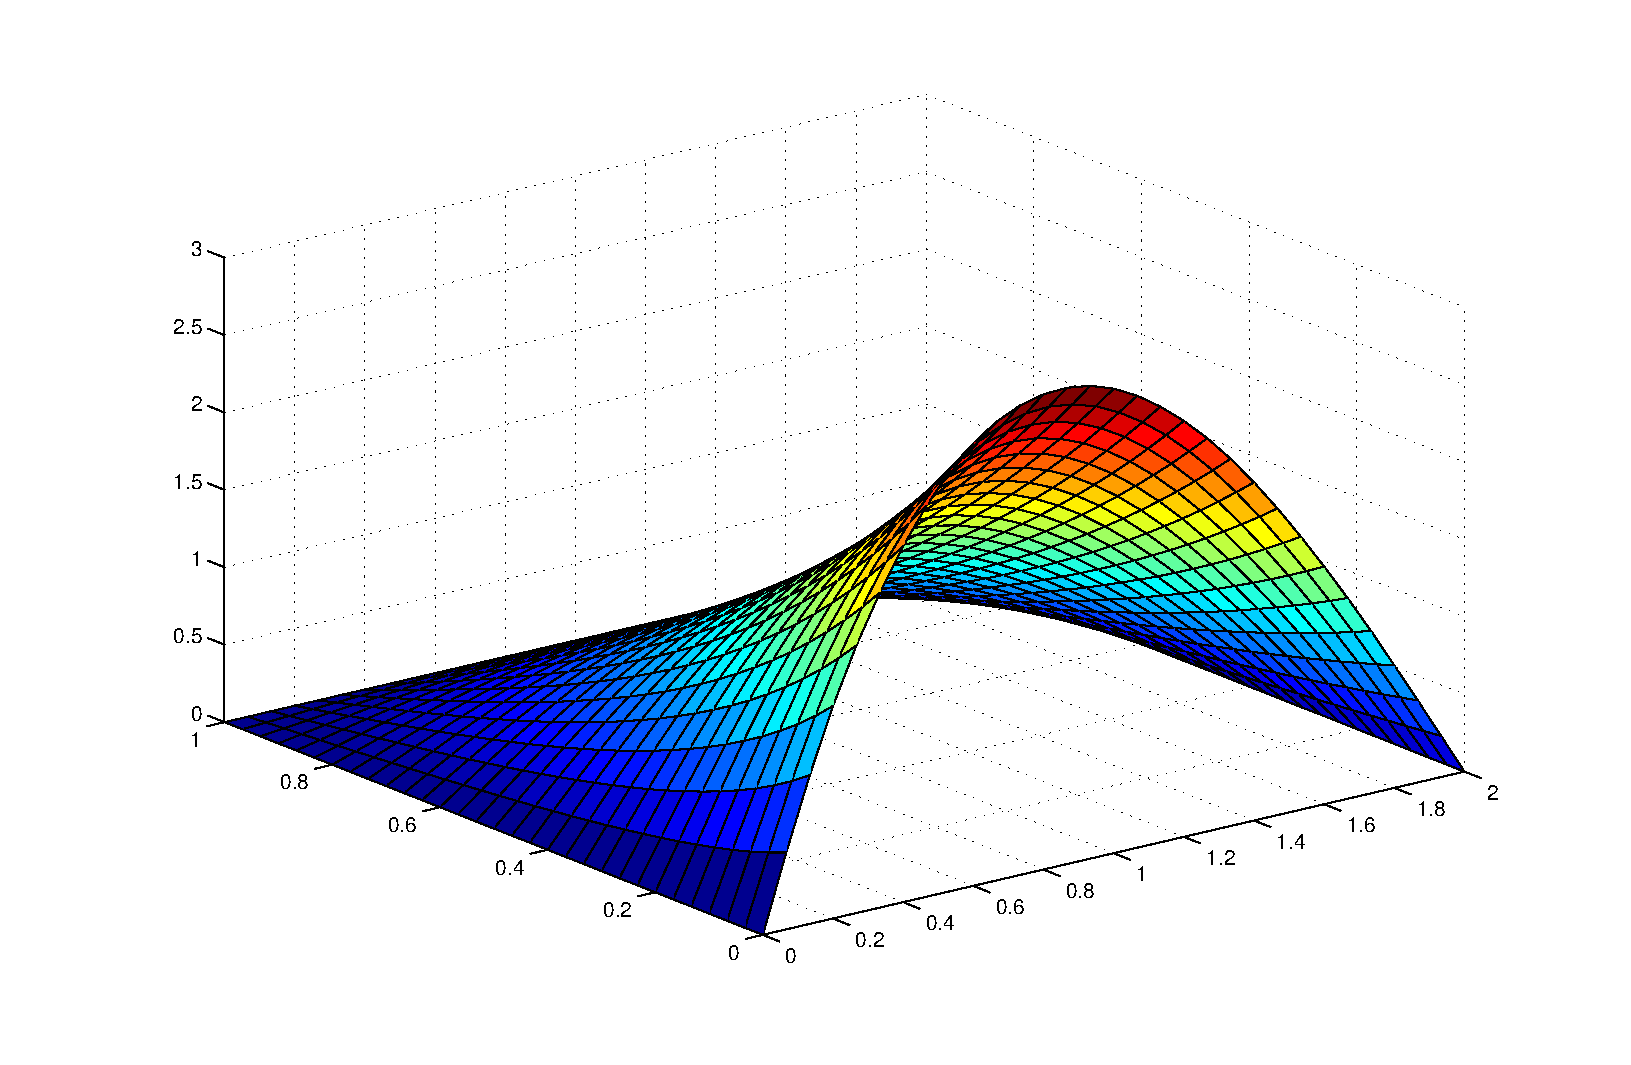
\includegraphics[bb=-78 148 689 643, width=5.67in, height=3.66in, keepaspectratio]{fig120305}}
    \caption{}
    \label{figure:12.3.5}
  \end{minipage}
  \begin{minipage}[b]{0.5\linewidth}
    \centering
    \scalebox{.65}{
    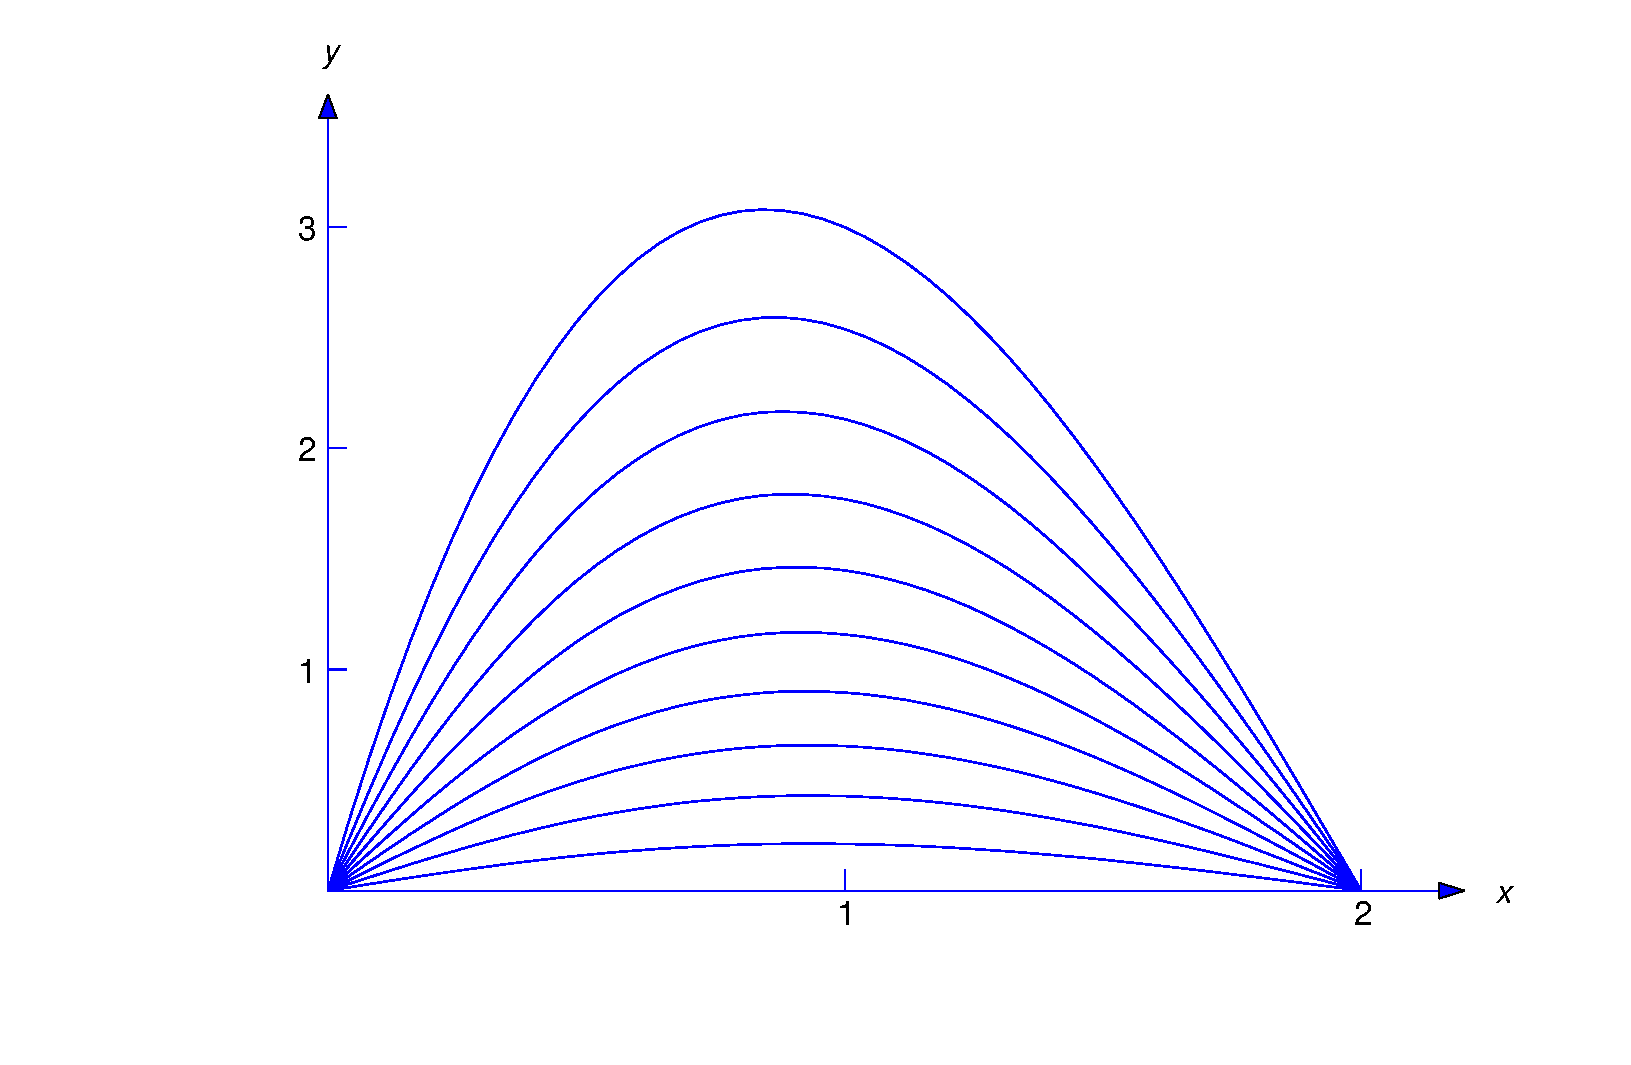
\includegraphics[bb=-78 148 689 643, width=5.67in, height=3.66in, keepaspectratio]{fig120306}}
    \caption{}
    \label{figure:12.3.6}
  \end{minipage}
\end{figure}
\end{examplesolution}

\setcounter{example}{2}
\setcounter{equation}{10}
\begin{example}
  \label{example:12.3.3} \rm Define the formal solution of
  \begin{equation}
    \label{eq:12.3.11}
    \begin{array}{c}
      u_{xx}+u_{yy}=0,\quad0<x<a,\quad0<y<b,           \\
      u(x,0)=0,\quad u_{y}(x,b)=f(x),\quad0\le x\le a, \\
      u_{x}(0,y)=0,\quad u_{x}(a,y)=0,\quad0\le y\le b
    \end{array}
  \end{equation}
  (Figure~12.3.7).
\end{example}
\setcounter{equation}{11}
\begin{examplesolution}
\solution The boundary conditions in \eqref{eq:12.3.11} require products $v(x,y)=X(x)Y(y)$ such that
$X'(0)=X'(a)=Y(0)=0$; hence, we let $k=-\lambda$ in \textup{(12.3.3)}. Thus, $X$ and $Y$ must
satisfy
\begin{equation}
  \label{eq:12.3.12}X''+\lambda X=0,\quad X'(0)=0,\quad X'(a)=0
\end{equation}
and
\begin{equation}
  \label{eq:12.3.13}Y''-\lambda Y=0,\quad Y(0)=0.
\end{equation}
From Theorem~11.1.3, the eigenvalues of \eqref{eq:12.3.12} are $\lambda=0$, with
associated eigenfunction $X_{0}=1$, and $\lambda_{n}=n^{2}\pi^{2}/a^{2}$, with associated
eigenfunctions
\[
  X_{n}=\cos\frac{n\pi x}{a},\quad n=1,2,3,\dots.
\]
Since $Y_{0}=y$ satisfies \eqref{eq:12.3.13} with $\lambda=0$, we take
$v_{0}(x,y)=X_{0}(x)Y_{0}(y)=y$. Substituting $\lambda=n^{2}\pi^{2}/a^{2}$ into \eqref{eq:12.3.13}
yields
\[
  Y''-(n^{2}\pi^{2}/a^{2})Y=0,\quad Y(0)=0,
\]
so we could take
\begin{equation}
  \label{eq:12.3.14}Y_{n}=\sinh\frac{n\pi y}{a}.
\end{equation}
However, because of the nonhomogeneous Neumann condition at $y=b$, it's better to require that
$Y_{n}'(b)=1$, which can be achieved by dividing the right side of \eqref{eq:12.3.14} by the value
of its derivative at $y=b$; thus,
\[
  Y_{n}=\frac{a\sinh n\pi y/a}{n\pi\cosh n\pi b/a}.
\]
Then
\[
  v_{n}(x,y)=X_{n}(x)Y_{n}(y)= \frac{a\sinh n\pi y/a}{n\pi\cosh n\pi b/a}\cos\frac{n\pi x}{a},
\]
so
\[
  \frac{\partial v_{n}}{\partial y}(x,b)=\cos\frac{n\pi x}{a}.
\]
Therefore $v_{n}$ satisfies \eqref{eq:12.3.11} with $f(x)=\cos n\pi x/a$. More generally, if
$\alpha_{0}$, \dots, $\alpha_{m}$ are arbitrary constants then
\[
  u_{m}(x,y)=\alpha_{0}y+\frac{a}{\pi}\sum_{n=1}^{m}\alpha_{n}\frac{\sinh n\pi y/a}{n\cosh n\pi b/a}\cos\frac{n\pi x}{a}
\]
satisfies \eqref{eq:12.3.11} with
\[
  f(x)=\alpha_{0}+\sum_{n=1}^{m}\alpha_{n}\cos\frac{n\pi x}{a}.
\]
Therefore, if $f$ is an arbitrary piecewise smooth function on $[0,a]$ we define the formal solution
of \eqref{eq:12.3.11} to be
\[
  u(x,y)=\alpha_{0}y+\frac{a}{\pi}\sum_{n=1}^{\infty}\alpha_{n}\frac{\sinh n\pi y/a}{n\cosh n\pi b/a}\cos\frac{n\pi x}{a},
\]
where
\[
  C(x)=\alpha_{0}+\sum_{n=1}^{\infty}\alpha_{n}\cos\frac{n\pi x}{a}
\]
is the Fourier cosine series of $f$ on $[0,a]$; that is,
\[
  \alpha_{0}=\frac{1}{a}\int_{0}^{a}f(x)\,dx \mbox{\quad and \quad}\alpha_{n}=\frac{2}{a}\int_{0}^{a}f(x)\cos\frac{n\pi x}{a}\,dx,\quad n=1,2,3,\dots.
\]
\end{examplesolution}

\setcounter{example}{3}
\begin{example}
  \label{example:12.3.4}\rm Solve \eqref{eq:12.3.11} with $f(x)=x$.
\end{example}
\setcounter{equation}{14}
\setcounter{figure}{7}
\begin{examplesolution}
\solution From Example~\ref{example:11.3.1},
\[
  C(x)=\dst\frac{a}{2}-\frac{4a}{\pi^{2}}\sum_{n=1}^{\infty}\frac{1}{(2n-1)^{2}}\cos\frac{(2n-1)\pi x}{a}.
\]
Therefore
\begin{equation}
  \label{eq:12.3.15}u(x,y)=\dst\frac{ay}{2}-\frac{4a^{2}}{\pi^{3}}\sum_{n=1}^{\infty}\frac{\sinh(2n-1)\pi y/a}{(2n-1)^{3}\cosh(2n-1)\pi b/a}\cos\frac{(2n-1)\pi x}{a}.
\end{equation}
For graphing purposes, we chose $a=2$, $b=1$, and retained the terms through $n=10$ in
\eqref{eq:12.3.15}. Figure~\ref{figure:12.3.8} shows the surface
\[
  u=u(x,y),\quad0\le x\le2,\quad0\le y\le1,
\]
while Figure~\ref{figure:12.3.9} shows the curves
\[
  u=u(x,.1k),\quad0\le x\le2,\quad k=0,1,\dots,10.
\]

\begin{figure}[H]
  \relax
  \begin{minipage}[b]{0.5\linewidth}
    \centering
    \scalebox{.65}{
    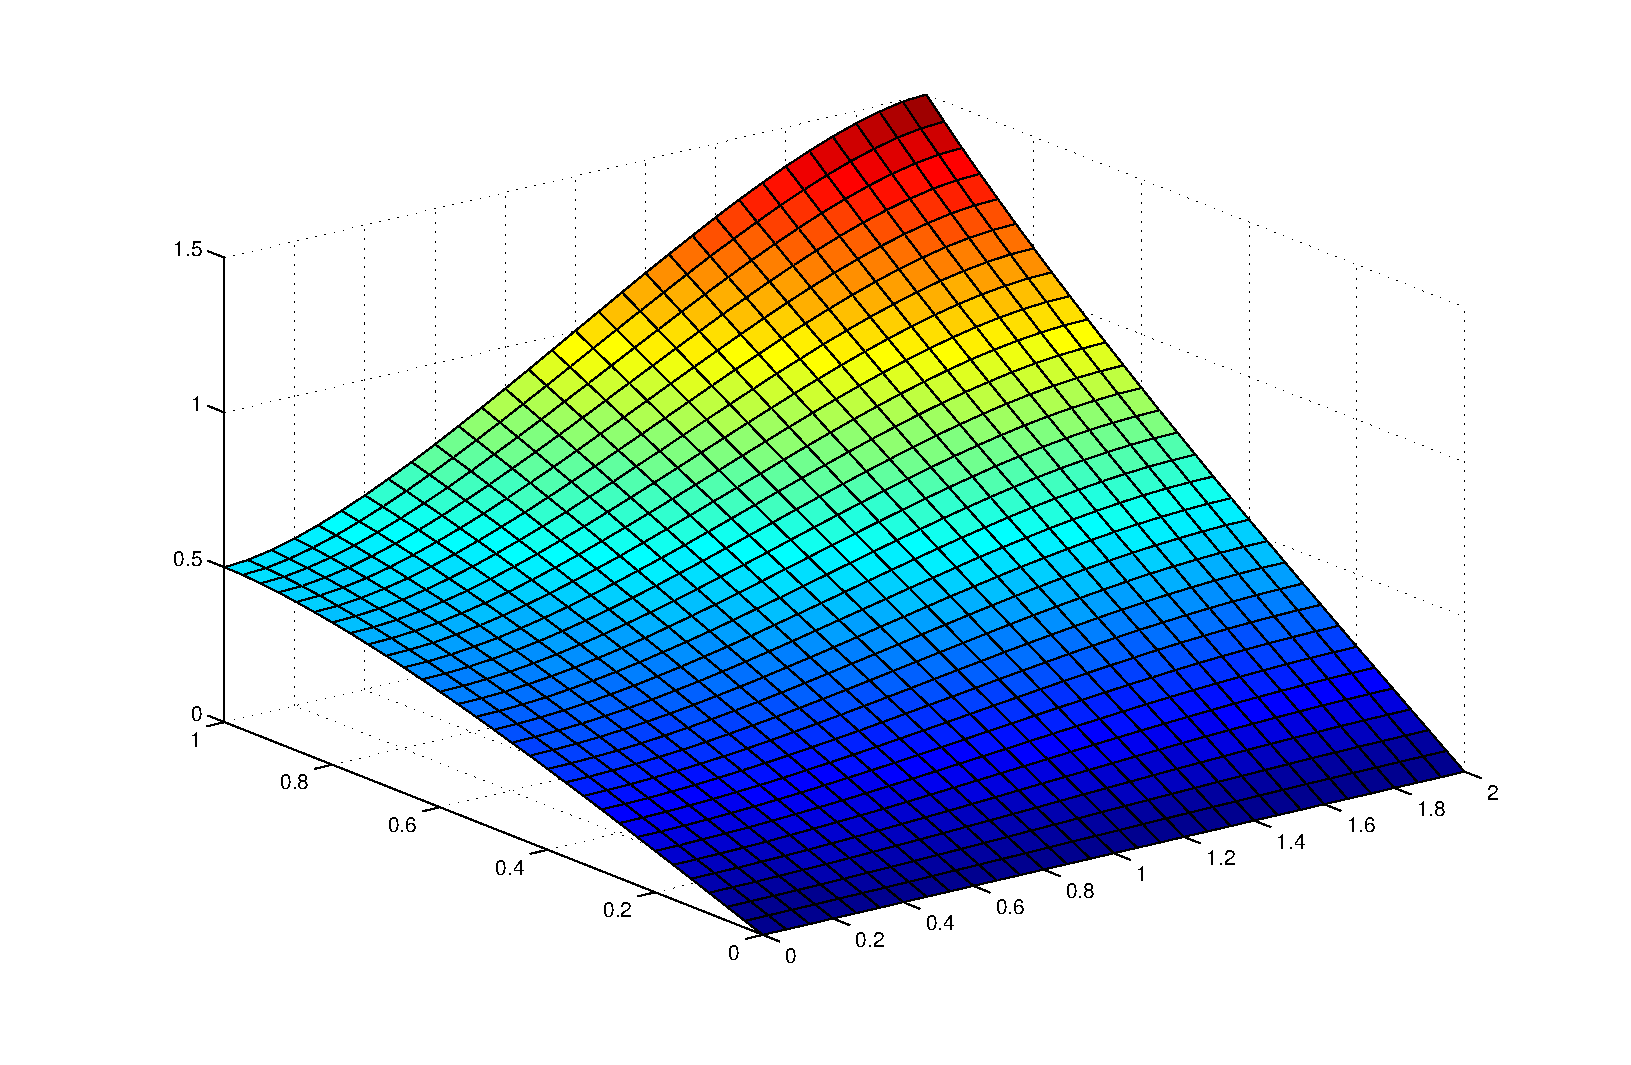
\includegraphics[bb=-78 148 689 643, width=5.67in, height=3.66in, keepaspectratio]{fig120308}}
    \caption{}
    \label{figure:12.3.8}
  \end{minipage}
  \begin{minipage}[b]{0.5\linewidth}
    \centering
    \scalebox{.65}{
    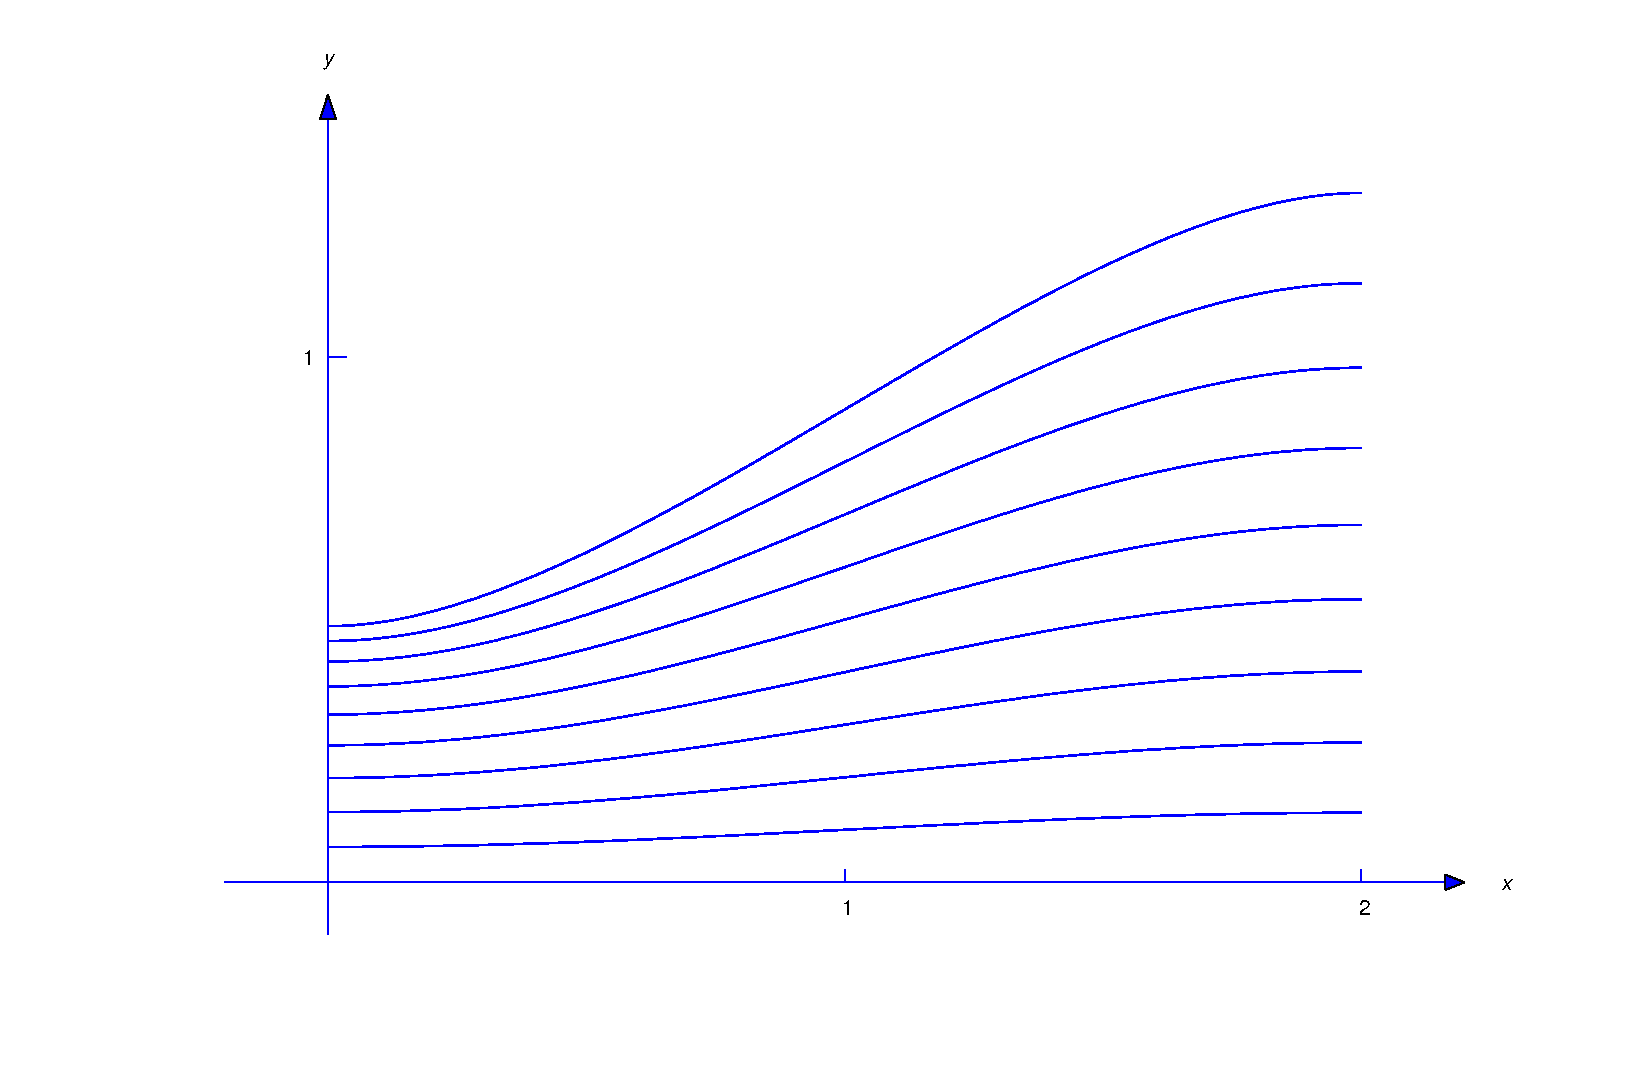
\includegraphics[bb=-78 148 689 643, width=5.67in, height=3.66in, keepaspectratio]{fig120309}}
    \caption{}
    \label{figure:12.3.9}
  \end{minipage}
\end{figure}
\end{examplesolution}

\setcounter{example}{4}
\setcounter{equation}{15}
\begin{example}
  \label{example:12.3.5} \rm Define the formal solution of
  \begin{equation}
    \label{eq:12.3.16}
    \begin{array}{c}
      u_{xx}+u_{yy}=0,\quad0<x<a,\quad0<y<b,          \\
      u(x,0)=0,\quad u_{y}(x,b)=0,\quad0\le x\le a,   \\
      u(0,y)=g(y),\quad u_{x}(a,y)=0,\quad0\le y\le b
    \end{array}
  \end{equation}
  (Figure~12.3.10).
\end{example}
\setcounter{equation}{16}
\begin{examplesolution}
\solution The boundary conditions in \eqref{eq:12.3.16} require products $v(x,y)=X(x)Y(y)$ such that
$Y(0)=Y'(b)=X'(a)=0$; hence, we let $k=\lambda$ in \textup{(12.3.3)}. Thus, $X$ and $Y$ must satisfy
\begin{equation}
  \label{eq:12.3.17}X''-\lambda X=0,\quad\quad X'(a)=0
\end{equation}
and
\begin{equation}
  \label{eq:12.3.18}Y''+\lambda Y=0,\quad Y(0)=0,\quad Y'(b)=0.
\end{equation}
From Theorem~11.1.4, the eigenvalues of \eqref{eq:12.3.18} are
$\lambda_{n}=(2n-1)^{2}\pi^{2}/4b^{2}$, with associated eigenfunctions
\[
  Y_{n}=\sin\frac{(2n-1)\pi y}{2b},\quad n=1,2,3,\dots.
\]
Substituting $\lambda=(2n-1)^{2}\pi^{2}/4b^{2}$ into \eqref{eq:12.3.17} yields
\[
  X''-((2n-1)^{2}\pi^{2}/4b^{2})X=0,\quad X'(a)=0,
\]
so we could take
\begin{equation}
  \label{eq:12.3.19}X_{n}=\cosh\frac{(2n-1)\pi(x-a)}{2b}.
\end{equation}
However, because of the nonhomogeneous Dirichlet condition at $x=0$, it's better to require that
$X_{n}(0)=1$, which can be achieved by dividing the right side of \eqref{eq:12.3.19} by its value at
$x=0$; thus,
\[
  X_{n}= \frac{\cosh(2n-1)\pi(x-a)/2b}{\cosh(2n-1)\pi a/2b}.
\]
Then
\[
  v_{n}(x,y)=X_{n}(x)Y_{n}(y)= \frac{\cosh(2n-1)\pi(x-a)/2b}{\cosh(2n-1)\pi a/2b}\sin\frac{(2n-1)\pi y}{2b},
\]
so
\[
  v_{n}(0,y)=\sin\frac{(2n-1)\pi y}{2b}.
\]
Therefore $v_{n}$ satisfies \eqref{eq:12.3.16} with $g(y)=\sin(2n-1)\pi y/2b$. More generally, if
$\alpha_{1}$, \dots, $\alpha_{m}$ are arbitrary constants then
\[
  u_{m}(x,y)=\sum_{n=1}^{m}\alpha_{n}\frac{\cosh(2n-1)\pi(x-a)/2b}{\cosh(2n-1)\pi a/2b}\sin\frac{(2n-1)\pi y}{2b}
\]
satisfies \eqref{eq:12.3.16} with
\[
  g(y)=\sum_{n=1}^{m}\alpha_{n}\sin\frac{(2n-1)\pi y}{2b}.
\]
Thus, if $g$ is an arbitrary piecewise smooth function on $[0,b]$, we define the formal solution of
\eqref{eq:12.3.16} to be
\[
  u(x,y)=\sum_{n=1}^{\infty}\alpha_{n}\frac{\cosh(2n-1)\pi(x-a)/2b}{\cosh(2n-1)\pi a/2b}\sin\frac{(2n-1)\pi y}{2b},
\]
where
\[
  S_{M}(y)=\sum_{n=1}^{\infty}\alpha_{n}\sin\frac{(2n-1)\pi y}{2b}
\]
is the mixed Fourier sine series of $g$ on $[0,b]$; that is,
\[
  \alpha_{n}=\frac{2}{b}\int_{0}^{b}g(y)\sin\frac{(2n-1)\pi y}{2b}\,dy.
\]
\end{examplesolution}

\setcounter{example}{5}
\begin{example}
  \label{example:12.3.6} \rm Solve \eqref{eq:12.3.16} with $g(y)=y(2y^{2}-9by+12b^{2})$.
\end{example}
\begin{examplesolution}
\solution From Example~\ref{example:11.3.8},
\[
  S_{M}(y) =\dst\frac{96b^{3}}{\pi^{3}}\sum_{n=1}^{\infty}\frac{1}{(2n-1)^{3}}\left[3+(-1)^{n}\frac{4}{(2n-1)\pi}\right]\sin\frac{(2n-1)\pi y}{2b}.
\]
Therefore
\[
  u(x,y) =\dst\frac{96b^{3}}{\pi^{3}}\sum_{n=1}^{\infty}\frac{\cosh(2n-1)\pi(x-a)/2b}{(2n-1)^{3}\cosh(2n-1)\pi a/2b}\left[3+(-1)^{n}\frac{4}{(2n-1)\pi}\right]\sin\frac{(2n-1)\pi y}{2b}.
\]
\end{examplesolution}

\setcounter{example}{6}
\setcounter{equation}{19}
\begin{example}
  \label{example:12.3.7} \rm Define the formal solution of
  \begin{equation}
    \label{eq:12.3.20}
    \begin{array}{c}
      u_{xx}+u_{yy}=0,\quad0<x<a,\quad0<y<b,              \\
      u_{y}(x,0)=0,\quad u(x,b)=0,\quad0\le x\le a,       \\
      u_{x}(0,y)=0,\quad u_{x}(a,y)=g(y),\quad0\le y\le b
    \end{array}
  \end{equation}
  (Figure~12.3.11).
\end{example}
\setcounter{equation}{20}
\begin{examplesolution}
\solution The boundary conditions in \eqref{eq:12.3.20} require products $v(x,y)=X(x)Y(y)$ such that
$Y'(0)=Y(b)=X'(0)=0$; hence, we let $k=\lambda$ in \textup{(12.3.3)}. Thus, $X$ and $Y$ must satisfy
\begin{equation}
  \label{eq:12.3.21}X''-\lambda X=0,\quad\quad X'(0)=0
\end{equation}
and
\begin{equation}
  \label{eq:12.3.22}Y''+\lambda Y=0,\quad Y'(0)=0,\quad Y(b)=0.
\end{equation}
From Theorem~11.1.4, the eigenvalues of \eqref{eq:12.3.22} are
$\lambda_{n}=(2n-1)^{2}\pi^{2}/4b^{2}$, with associated eigenfunctions
\[
  Y_{n}=\cos\frac{(2n-1)\pi y}{2b},\quad n=1,2,3,\dots.
\]
Substituting $\lambda=(2n-1)^{2}\pi^{2}/4b^{2}$ into \eqref{eq:12.3.21} yields
\[
  X''-((2n-1)^{2}\pi^{2}/4b^{2})X=0,\quad X'(0)=0,
\]
so we could take
\begin{equation}
  \label{eq:12.3.23}X_{n}=\cosh\frac{(2n-1)\pi x}{2b}.
\end{equation}
However, because of the nonhomogeneous Neumann condition at $x=a$, it's better to require that
$X_{n}'(a)=1$, which can be achieved by dividing the right side of \eqref{eq:12.3.23} by the value
of its derivative at $x=a$; thus,
\[
  X_{n}= \frac{2b\cosh(2n-1)\pi x/2b}{(2n-1)\pi\sinh(2n-1)\pi a/2b}.
\]
Then
\[
  v_{n}(x,y)=X_{n}(x)Y_{n}(y)= \frac{2b\cosh(2n-1)\pi x/2b}{(2n-1)\pi\sinh(2n-1)\pi a/2b}\cos\frac{(2n-1)\pi y}{2b},
\]
so
\[
  \frac{\partial v_{n}}{\partial x}(a,y)=\cos\frac{(2n-1)\pi y}{2b}.
\]
Therefore $v_{n}$ satisfies \eqref{eq:12.3.20} with $g(y)=\cos(2n-1)\pi y/2b$. More generally, if
$\alpha_{1}$, \dots, $\alpha_{m}$ are arbitrary constants then
\[
  u_{m}(x,y)=\frac{2b}{\pi}\sum_{n=1}^{m}\alpha_{n}\frac{\cosh(2n-1)\pi x/2b}{(2n-1)\sinh(2n-1)\pi a/2b}\cos\frac{(2n-1)\pi y}{2b}
\]
satisfies \eqref{eq:12.3.20} with
\[
  g(y)=\sum_{n=1}^{m}\alpha_{n}\cos\frac{(2n-1)\pi y}{2b}.
\]
Therefore, if $g$ is an arbitrary piecewise smooth function on $[0,b]$, we define the formal
solution of \eqref{eq:12.3.20} to be
\[
  u(x,y)=\frac{2b}{\pi}\sum_{n=1}^{\infty}\alpha_{n}\frac{\cosh(2n-1)\pi x/2b}{(2n-1)\sinh(2n-1)\pi a/2b}\cos\frac{(2n-1)\pi y}{2b},
\]
where
\[
  C_{M}(y)=\sum_{n=1}^{\infty}\alpha_{n}\cos\frac{(2n-1)\pi y}{2b}
\]
is the mixed Fourier cosine series of $g$ on $[0,b]$; that is,
\[
  \alpha_{n}=\frac{2}{b}\int_{0}^{b}g(y)\cos\frac{(2n-1)\pi y}{2b}\,dy.
\]
\end{examplesolution}

\setcounter{example}{7}
\begin{example}
  \label{example:12.3.8} \rm Solve \eqref{eq:12.3.20} with $g(y)=y-b$.
\end{example}
\begin{examplesolution}
\solution From Example~\ref{example:11.3.3},
\[
  C_{M}(y)=-\frac{8b}{\pi^{2}}\sum_{n=1}^{\infty}\frac{1}{(2n-1)^{2}}\cos\frac{(2n-1)\pi y}{2b}.
\]
Therefore
\[
  u(x,y)=-\frac{16b^{2}}{\pi^{3}}\sum_{n=1}^{\infty}\frac{\cosh(2n-1)\pi x/2b}{(2n-1)^{3}\sinh(2n-1)\pi a/2b}\cos\frac{(2n-1)\pi y}{2b}. \eqno{\bbox}
\]
\end{examplesolution}

\setcounter{example}{8}
\begin{example}
  \label{example:12.3.9} \rm Define the bounded formal solution of \textup{(12.3.24)}.
\end{example}
\begin{examplesolution}
\solution Proceeding as in the solution of Example~\ref{example:12.3.1}, we find that the building
block functions are of the form
\[
  v_{n}(x,y)=Y_{n}(y)\sin\frac{n\pi x}{a},
\]
where
\[
  Y_{n}''-(n^{2}\pi^{2}/a^{2})Y_{n}=0.
\]
Therefore
\[
  Y_{n}=c_{1}e^{n\pi y/a}+c_{2}e^{-n\pi y/a}
\]
where $c_{1}$ and $c_{2}$ are constants. Although the boundary conditions in \textup{(12.3.24)}
don't restrict $c_{1}$, and $c_{2}$, we must set $c_{1}=0$ to ensure that $Y_{n}$ is bounded.
Letting $c_{2}=1$ yields
\[
  v_{n}(x,y)=e^{-n\pi y/a}\sin\frac{n\pi x}{a},
\]
and we define the bounded formal solution of \textup{(12.3.24)} to be
\[
  u(x,y)=\sum_{n=1}^{\infty}b_{n}e^{-n\pi y/a}\sin\frac{n\pi x}{a},
\]
where
\[
  S(x)=\sum_{n=1}^{\infty}b_{n}\sin\frac{n\pi x}{a}
\]
is the Fourier sine series of $f$ on $[0,a]$. \bbox
\end{examplesolution}

\section*{Section 12.4}
\setcounter{chapter}{12}
\setcounter{section}{4}

\setcounter{example}{0}
\begin{example}
  \label{example:12.4.1} \rm Find the bounded formal solution of \textup{(12.4.2)} with
  $f(\theta)=\theta(\pi^{2}-\theta^{2})$.
\end{example}
\begin{examplesolution}
\solution From Example~\ref{example:11.2.6},
\[
  \theta(\pi^{2}-\theta^{2})=12\sum_{n=1}^{\infty}\frac{(-1)^{n}}{n^{3}}\sin n\theta,\quad-\pi\le\theta\le\pi,
\]
so
\[
  u(r,\theta)=12\sum_{n=1}^{\infty}\frac{r^{n}}{\rho^{n}}\frac{(-1)^{n}}{n^{3}}\sin n\theta,\quad 0\le r\le\rho,\quad-\pi\le\theta\le\pi.
\]
\end{examplesolution}

\setcounter{example}{1}
\setcounter{equation}{8}
\begin{example}
  \label{example:12.4.2} \rm Define the formal solution of
  \begin{equation}
    \label{eq:12.4.9}
    \begin{array}{c}
      \dst u_{rr}+\frac{1}{r}u_{r}+\frac{1}{r^{2}}u_{\theta\theta}=0,\quad \rho_{0}<r<\rho,\quad-\pi\le\theta<\pi, \\[2\jot]
      u(\rho_{0},\theta)=0,\quad u(\rho,\theta)=f(\theta),\quad -\pi\le\theta<\pi,
    \end{array}
  \end{equation}
  where $0<\rho_{0}<\rho$ (Figure~12.4.2).
\end{example}
\begin{examplesolution}
\solution We use separation of variables exactly as before, except that now we choose the constants
in \textup{(12.4.5)} and \textup{(12.4.7)} so that $R_{n}(\rho_{0})=0$ for $n=0$, $1$, $2$,\dots. In
view of the nonhomogeneous Dirichlet condition on the boundary $r=\rho$, it's also convenient to
require that $R_{n}(\rho)=1$ for $n=0$, $1$, $2$,\dots. We leave it to you to verify that
\[
  R_{0}(r)=\frac{\ln(r/\rho_{0})}{\ln(\rho/\rho_{0})}\mbox{\quad and \quad}R_{n}=\frac{\rho_{0}^{-n}r^{n}-\rho_{0}^{n}r^{-n}}{\rho_{0}^{-n}\rho^{n}-\rho_{0}^{n}\rho^{-n}},\quad n=1,2,3,\dots
\]
satisfy these requirements. Therefore
\[
  v_{0}(r,\theta)=\frac{\ln(r/\rho_{0})}{\ln(\rho/\rho_{0})}
\]
and
\[
  v_{n}(r,\theta)=\frac{\rho_{0}^{-n}r^{n}-\rho_{0}^{n}r^{-n}}{\rho_{0}^{-n}\rho^{n}-\rho_{0}^{n}\rho^{-n}}(\alpha_{n}\cos n\theta+\beta_{n}\sin n\theta), \quad n=1,2,3,\dots,
\]
where $\alpha_{n}$ and $\beta_{n}$ are arbitrary constants.

If $\alpha_{0}$, $\alpha_{1}$,\dots, $\alpha_{m}$ and $\beta_{1}$, $\beta_{2}$, \dots, $\beta_{m}$
are arbitrary constants then
\[
  u_{m}(r,\theta)=\alpha_{0}\frac{\ln(r/\rho_{0})}{\ln(\rho/\rho_{0})}+ \sum_{n=1}^{m}\frac{\rho_{0}^{-n}r^{n}-\rho_{0}^{n}r^{-n}}{\rho_{0}^{-n}\rho^{n}-\rho_{0}^{n}\rho^{-n}}(\alpha_{n}\cos n\theta+\beta_{n}\sin n\theta)
\]
satisfies \eqref{eq:12.4.9}, with
\[
  f(\theta) =\alpha_{0}+\sum_{n=1}^{m}(\alpha_{n}\cos n\theta+\beta_{n}\sin n\theta).
\]
This motivates us to define the formal solution of \eqref{eq:12.4.9} for general $f$ to be
\[
  u(r,\theta)=\alpha_{0}\frac{\ln(r/\rho_{0})}{\ln(\rho/\rho_{0})}+ \sum_{n=1}^{\infty}\frac{\rho_{0}^{-n}r^{n}-\rho_{0}^{n}r^{-n}}{\rho_{0}^{-n}\rho^{n}-\rho_{0}^{n}\rho^{-n}}(\alpha_{n}\cos n\theta+\beta_{n}\sin n\theta),
\]
where
\[
  F(\theta) =\alpha_{0}+\sum_{n=1}^{\infty}(\alpha_{n}\cos n\theta+\beta_{n}\sin n\theta)
\]
is the Fourier series of $f$ on $[-\pi,\pi]$.
\end{examplesolution}

\setcounter{example}{2}
\setcounter{equation}{9}
\begin{example}
  \label{example:12.4.3} \rm Define the bounded formal solution of
  \begin{equation}
    \label{eq:12.4.10}
    \begin{array}{c}
      \dst u_{rr}+\frac{1}{r}u_{r}+\frac{1}{r^{2}}u_{\theta\theta}=0,\quad 0<r<\rho,\quad0<\theta<\gamma, \\[2\jot]
      u(\rho,\theta)=f(\theta),\quad0\le\theta\le\gamma,                                                  \\[2\jot]
      u(r,0)=0,\quad u(r,\gamma)=0,\quad0<r<\rho,
    \end{array}
  \end{equation}
  where $0<\gamma<2\pi$ (Figure~12.4.3).
\end{example}
\setcounter{equation}{10}
\begin{examplesolution}
\solution Now $v(r,\theta)=R(r)\Theta(\theta)$, where
\begin{equation}
  \label{eq:12.4.11}r^{2}R''+rR'-\lambda R=0
\end{equation}
and
\begin{equation}
  \label{eq:12.4.12}\Theta''+\lambda\Theta=0,\quad\Theta(0)=0,\quad\Theta(\gamma)=0.
\end{equation}
From Theorem~11.1.2, the eigenvalues of \eqref{eq:12.4.12} are
$\lambda_{n}=n^{2}\pi^{2}/\gamma^{2}$, with associated eigenfunction
$\Theta_{n}=\sin n\pi\theta/\gamma$, $n=1$, $2$, $3$,\dots. Substituting
$\lambda=n^{2}\pi^{2}/\gamma^{2}$ into \eqref{eq:12.4.11} yields the Euler equation
\[
  r^{2}R_{n}''+rR_{n}'-\frac{n^{2}\pi^{2}}{\gamma^{2}}R_{n}=0.
\]
The indicial polynomial of this equation is
\[
  s(s-1)+s-\frac{n^{2}\pi^{2}}{\gamma^{2}}=\left(s-\frac{n\pi}{\gamma}\right) \left(s+\frac{n\pi}{\gamma}\right),
\]
so
\[
  R_{n}=c_{1}r^{n\pi/\gamma}+c_{2}r^{-n\pi/\gamma},
\]
by Theorem~7.4.3. To obtain a solution that remains bounded as $r\to0+$ we let
$c_{2}=0$. Because of the Dirichlet condition at $r=\rho$, it's convenient to have $R_{n}(\rho)=1$;
therefore we take $c_{1}=\rho^{-n\pi/\gamma}$, so
\[
  R_{n}(r)=\frac{r^{n\pi/\gamma}}{\rho^{n\pi/\gamma}}.
\]
Now
\[
  v_{n}(r,\theta)=R_{n}(r)\Theta_{n}(\theta)=\frac{r^{n\pi/\gamma}}{\rho^{n\pi/\gamma}}\sin\frac{n\pi\theta}{\gamma}
\]
satisfies \eqref{eq:12.4.10} with
\[
  f(\theta)=\sin\frac{n\pi\theta}{\gamma}.
\]
More generally, if $\alpha_{1}$, $\alpha_{2}$, \dots, $\alpha_{m}$ are arbitrary constants then
\[
  u_{m}(r,\theta)=\sum_{n=1}^{m}\alpha_{n}\frac{r^{n\pi/\gamma}}{\rho^{n\pi/\gamma}}\sin\frac{n\pi\theta}{\gamma}
\]
satisfies \eqref{eq:12.4.10} with
\[
  f(\theta) =\sum_{n=1}^{m}\alpha_{n}\sin\frac{n\pi\theta}{\gamma}.
\]
This motivates us to define the bounded formal solution of \eqref{eq:12.4.10} to be
\[
  u(r,\theta)=\sum_{n=1}^{\infty}\alpha_{n}\frac{r^{n\pi/\gamma}}{\rho^{n\pi/\gamma}}\sin\frac{n\pi\theta}{\gamma},
\]
where
\[
  S(\theta)=\sum_{n=1}^{\infty}\alpha_{n}\sin\frac{n\pi\theta}{\gamma}
\]
is the Fourier sine expansion of $f$ on $[0,\gamma]$; that is,
\[
  \alpha_{n}=\frac{2}{\gamma}\int_{0}^{\gamma}f(\theta)\sin\frac{n\pi\theta}{\gamma}\,d\theta.
\]
\end{examplesolution}

\section*{Section 13.1}
\phantomsection
\addcontentsline{toc}{chapter}{Chapter 13}
\setcounter{chapter}{13}
\setcounter{section}{1}

\setcounter{example}{0}
\begin{example}
  \label{example:13.1.1} \rm Consider the boundary value problem
  \[
    y''+y=1,\quad y(0)=0,\quad y(\pi/2)=0.
  \]
  The general solution of $y''+y=1$ is
  \[
    y=1+c_{1}\sin x+c_{2}\cos x,
  \]
  so $y(0)=0$ if and only if $c_{2}=-1$ and $y(\pi/2)=0$ if and only if $c_{1}=-1$. Therefore
  \[
    y=1-\sin x-\cos x
  \]
  is the unique solution of the boundary value problem.
\end{example}

\setcounter{example}{1}
\begin{example}
  \label{example:13.1.2} \rm Consider the boundary value problem
  \[
    y''+y=1,\quad y(0)=0,\quad y(\pi)=0.
  \]
  Again, the general solution of $y''+y=1$ is
  \[
    y=1+c_{1}\sin x+c_{2}\cos x,
  \]
  so $y(0)=0$ if and only if $c_{2}=-1$, but $y(\pi)=0$ if and only if $c_{2}=1$. Therefore the
  boundary value problem has no solution.
\end{example}

\setcounter{example}{2}
\begin{example}
  \label{example:13.1.3} \rm Consider the boundary value problem
  \[
    y''+y=\sin2x,\quad y(0)=0,\quad y(\pi)=0.
  \]
  You can use the method of undetermined coefficients (Section~5.5) to find that the general
  solution of $y''+y=\sin2x$ is
  \[
    y=-\frac{\sin2x}{3}+c_{1}\sin x+c_{2}\cos x.
  \]
  The boundary conditions $y(0)=0$ and $y(\pi)=0$ both require that $c_{2}=0$, but they don't
  restrict $c_{1}$. Therefore the boundary value problem has infinitely many solutions
  \[
    y=-\frac{\sin2x}{3}+c_{1}\sin x,
  \]
  where $c_{1}$ is arbitrary.
\end{example}

\setcounter{example}{3}
\setcounter{equation}{12}
\begin{example}
  \label{example:13.1.4} \rm Solve the boundary value problem
  \begin{equation}
    \label{eq:13.1.13}x^{2}y''-2xy'+2y-2x^{3}=0,\quad y(1)=4,\quad y'(2)=3,
  \end{equation}
  given that $\{x,x^{2}\}$ is a fundamental set of solutions of the complementary equation. \end{example}
\begin{examplesolution}
\solution Using variation of parameters (Section~5.7), you can show that $y_{p}=x^{3}$ is a solution
of the nonhomogeneous equation
\[
  x^{2}y''-2xy'+2y=2x^{3}.
\]
Therefore the solution of \eqref{eq:13.1.13} can be written as
\[
  y=x^{3}+c_{1}x+c_{2}x^{2}.
\]
Then
\[
  y'=3x^{2}+c_{1}+2c_{2}x,
\]
and imposing the boundary conditions yields the system
\begin{eqnarray*}
  c_{1}+\phantom{4}c_{2} & = & \phantom{-}3 \\
  c_{1}+4c_{2}           & = & -9,
\end{eqnarray*}
so $c_{1}=7$ and $c_{2}=-4$. Therefore
\[
  y=x^{3}+7x-4x^{2}
\]
is the unique solution of \eqref{eq:13.1.13}.
\end{examplesolution}

\setcounter{example}{4}
\begin{example}
  \label{example:13.1.5} \rm Solve the boundary value problem
  \[
    y''-7y'+12y=4e^{2x},\quad y(0)=3,\quad y(1)=5e^{2}.
  \]
\end{example}
\setcounter{equation}{13}
\begin{examplesolution}
\solution From Example~\ref{example:5.4.1}, $y_{p}=2e^{2x}$ is a particular solution of
\begin{equation}
  \label{eq:13.1.14}y''-7y'+12y=4e^{2x}.
\end{equation}
Since $\{e^{3x},e^{4x}\}$ is a fundamental set for the complementary equation, we could write the
solution of \eqref{eq:13.1.14} as
\[
  y=2e^{2x}+c_{1}e^{3x}+c_{2}e^{4x}
\]
and determine $c_{1}$ and $c_{2}$ by imposing the boundary conditions. However, this would lead to
some tedious algebra, and the form of the solution would be very unappealing. (Try it!) In this case
it's convenient to use the fundamental system $\{z_{1},z_{2}\}$ mentioned in
Theorem~13.1.2\part{e}; that is, we choose $\{z_{1},z_{2}\}$ so that
$B_{1}(z_{1})=z_{1}(0)=0$ and $B_{2}(z_{2})=z_{2}(1)=0$. It is easy to see that
\[
  z_{1}=e^{3x}-e^{4x}\text{\; and\; \; }z_{2}=e^{3(x-1)}-e^{4(x-1)}
\]
satisfy these requirements. Now we write the solution of \eqref{eq:13.1.14} as
\[
  y=2e^{2x}+c_{1}\left(e^{3x}-e^{4x}\right)+c_{2}\left(e^{3(x-1)}-e^{4(x-1)}\right).
\]
Imposing the boundary conditions $y(0)=3$ and $y(1)=5e^{2}$ yields
\[
  3=2+c_{2}e^{-4}(e-1)\text{\; and\; \; }5e^{2}=2e^{2}+c_{1}e^{3}(1-e).
\]
Therefore
\[
  c_{1}=\frac{3}{e(1-e)},\quad c_{2}=\frac{e^{4}}{e-1},
\]
and
\[
  y=2e^{2x}+\frac{3}{e(1-e)}(e^{3x}-e^{4x})+ \frac{e^{4}}{e-1}(e^{3(x-1)}-e^{4(x-1)}).
\]
\end{examplesolution}

\setcounter{example}{5}
\setcounter{equation}{20}
\begin{example}
  \label{example:13.1.6}\rm Solve the boundary value problem
  \begin{equation}
    \label{eq:13.1.21}y''+y=F(x),\quad y(0)+y'(0)=0,\quad y(\pi)-y'(\pi)=0,
  \end{equation}
  and find the Green's function for this problem.
\end{example}
\begin{examplesolution}
\solution Here
\[
  B_{1}(y)=y(0)+y'(0)\text{\; and\; \; }B_{2}(y)=y(\pi)-y'(\pi).
\]
Let $\{z_{1},z_{2}\}=\{\cos x,\sin x\}$, which is a fundamental set of solutions of $y''+y=0$. Then
\begin{eqnarray*}
  B_{1}(z_{1}) & = & (\cos x-\sin x)\big|_{x=0}=\phantom{-}1 \\
  B_{2}(z_{1}) & = & (\cos x+\sin x)\big|_{x=\pi}=-1
\end{eqnarray*}
and
\begin{eqnarray*}
  B_{1}(z_{2}) & = & (\sin x+\cos x)\big|_{x=0}=1 \\
  B_{2}(z_{2}) & = & (\sin x-\cos x)\big|_{x=\pi}=1.
\end{eqnarray*}
Therefore
\[
  B_{1}(z_{1})B_{2}(z_{2})-B_{1}(z_{2})B_{2}(z_{1})=2,
\]
so Theorem~13.1.2 implies that \eqref{eq:13.1.21} has a unique solution. Let
\[
  y_{1}=B_{1}(z_{2})z_{1}-B_{1}(z_{1})z_{2}=\cos x-\sin x
\]
and
\[
  y_{2}=B_{2}(z_{2})z_{1}-B_{2}(z_{1})z_{2}=\cos x+\sin x.
\]
Then $B_{1}(y_{1})=0$, $B_{2}(y_{2})=0$, and the Wronskian of $\{y_{1},y_{2}\}$ is
\[
  W(x)= \left|
  \begin{array}{rrccccc}
    \cos x-\sin x  & \cos x+\sin x  \\
    -\sin x-\cos x & -\sin x+\cos x
  \end{array}\right|=2.
\]
Since $P_{0}=1$, \textup{(13.1.17)} yields the solution
\begin{eqnarray*}
  y(x) & = & \dst{\frac{\cos x-\sin x}{2}}\int_{x}^{\pi}F(t)(\cos t+\sin t)\,dt \\
       &   & +\dst{\frac{\cos x+\sin x}{2}}\int_{0}^{x}F(t)(\cos t-\sin t)\,dt.
\end{eqnarray*}
The Green's function is
\[
  G(x,t)=
  \begin{cases}
    \dst{\frac{(\cos t-\sin t)(\cos x+\sin x)}{2}}, & \quad0\le t\le x,   \\[.1in]
    \dst{\frac{(\cos x-\sin x)(\cos t+\sin t)}{2}}, & \quad x\le t\le\pi.
  \end{cases}
\]
\end{examplesolution}

\setcounter{example}{6}
\setcounter{equation}{24}
\begin{example}
  \label{example:13.1.7} \rm Applying Theorem~13.1.4 to the boundary value problem
  \begin{equation}
    \label{eq:13.1.25}y''+y=F(x),\quad y(0)=0,\quad y(\pi)=0
  \end{equation}
  explains the Examples~\ref{example:13.1.2} and \ref{example:13.1.3}. The complementary equation
  $y''+y=0$ has the linearly independent solutions $y_{1}=\sin x$ and $y_{2}=\cos x$, and $y_{1}$
  satisfies both boundary conditions. Since $P_{0}=1$ and
  \[
    W= \left|
    \begin{array}{crccccc}
      \sin x & \cos x  \\
      \cos x & -\sin x
    \end{array}\right|=-1,
  \]
  \textup{(13.1.23)} reduces to
  \[
    \int_{0}^{\pi}F(x)\sin x\,dx=0.
  \]
  From Example~\ref{example:13.1.2}, $F(x)=1$ and
  \[
    \int_{0}^{\pi}F(x)\sin x\,dx=\int_{0}^{\pi}\sin x\,dx=2,
  \]
  so Theorem~13.1.4 implies that \eqref{eq:13.1.25} has no solution. In
  Example~\ref{example:13.1.3},
  \[
    F(x)=\sin2x=2\sin x\cos x
  \]
  and
  \[
    \int_{0}^{\pi}F(x)\sin x\,dx=2\int_{0}^{\pi}\sin^{2}x\cos x\,dx =\frac{2}{3}\sin^{3}x\bigg|_{0}^{\pi}=0,
  \]
  so Theorem~13.1.4 implies that \eqref{eq:13.1.25} has infinitely many solutions,
  differing by constant multiples of $y_{1}(x)=\sin x$.
\end{example}

\section*{Section 13.2}
\setcounter{chapter}{13}
\setcounter{section}{2}

\setcounter{example}{0}
\setcounter{equation}{1}
\begin{example}
  \label{example:13.2.1} \rm Solve the eigenvalue problem
  \begin{equation}
    \label{eq:13.2.2}y''+3y'+2y+\lambda y=0,\quad y(0)=0,\quad y(1)=0.
  \end{equation}
\end{example}
\setcounter{equation}{2}
\begin{examplesolution}
\solution The characteristic equation of \eqref{eq:13.2.2} is
\[
  r^{2}+3r+2+\lambda=0,
\]
with zeros
\[
  r_{1}=\frac{-3+\sqrt{1-4\lambda}}{2}\text{\quad and \quad }r_{2}=\frac{-3-\sqrt{1-4\lambda}}{2}.
\]
If $\lambda<1/4$ then $r_{1}$ and $r_{2}$ are real and distinct, so the general solution of the
differential equation in \eqref{eq:13.2.2} is
\[
  y=c_{1}e^{r_{1}x}+c_{2}e^{r_{2}x}.
\]
The boundary conditions require that
\begin{eqnarray*}
  c_{1}\phantom{e^{r_{1}}}+c_{2}\phantom{e^{r_{2}}} & = & 0 \\
  c_{1}e^{r_{1}}+c_{2}e^{r_{2}}                     & = & 0.
\end{eqnarray*}
Since the determinant of this system is $e^{r_{2}}-e^{r_{1}}\ne0$, the system has only the trivial
solution. Therefore $\lambda$ isn't an eigenvalue of \eqref{eq:13.2.2}.

If $\lambda=1/4$ then $r_{1}=r_{2}=-3/2$, so the general solution of \eqref{eq:13.2.2} is
\[
  y=e^{-3x/2}(c_{1}+c_{2}x).
\]
The boundary condition $y(0)=0$ requires that $c_{1}=0$, so $y=c_{2}xe^{-3x/2}$ and the boundary
condition $y(1)=0$ requires that $c_{2}=0$. Therefore $\lambda=1/4$ isn't an eigenvalue
of~\eqref{eq:13.2.2}.

If $\lambda>1/4$ then
\[
  r_{1}=-\frac{3}{2}+i\omega\text{\quad and\quad }r_{2}=-\frac{3}{2}-i\omega,
\]
with
\begin{equation}
  \label{eq:13.2.3}\omega=\frac{\sqrt{4\lambda-1}}{2}\text{\quad or, equivalently,\quad }\lambda=\frac{1+4\omega^{2}}{4}.
\end{equation}
In this case the general solution of the differential equation in \eqref{eq:13.2.2} is
\[
  y=e^{-3x/2}(c_{1}\cos\omega x+c_{2}\sin\omega x).
\]
The boundary condition $y(0)=0$ requires that $c_{1}=0$, so $y=c_{2}e^{-3x/2}\sin\omega x$. The condition $y(1)=0$
holds with $c_{2}\ne0$ if and only if $\omega=n\pi$, where $n$ is an integer. We may assume that $n$
is a positive integer. (Why?). From \eqref{eq:13.2.3}, the eigenvalues are
$\lambda_{n}=(1+4n^{2}\pi^{2})/4$, with associated eigenfunctions
\[
  y_{n}=e^{-3x/2}\sin n\pi x,\quad n=1,2,3,\dots.
\]
\end{examplesolution}

\setcounter{example}{1}
\setcounter{equation}{3}
\begin{example}
  \label{example:13.2.2} \rm Solve the eigenvalue problem
  \begin{equation}
    \label{eq:13.2.4}x^{2}y''+xy'+\lambda y=0,\quad y(1)=0,\quad y(2)=0.
  \end{equation}
\end{example}
\begin{examplesolution}
\solution If $\lambda=0$, the differential equation in \eqref{eq:13.2.4} reduces to $x(xy')'=0$, so
$xy'=c_{1}$,
\[
  y'=\frac{c_{1}}{x},\text{\quad and\quad}y=c_{1}\ln x+c_{2}.
\]
The boundary condition $y(1)=0$ requires that $c_{2}=0$, so $y=c_{1}\ln x$. The boundary condition
$y(2)=0$ requires that $c_{1}\ln2=0$, so $c_{1}=0$. Therefore zero isn't an eigenvalue of
\eqref{eq:13.2.4}.

If $\lambda<0$, we write $\lambda=-k^{2}$ with $k>0$, so \eqref{eq:13.2.4} becomes
\[
  x^{2}y''+xy'-k^{2}y=0,
\]
an Euler equation (Section~7.4) with indicial equation
\[
  r^{2}-k^{2}=(r-k)(r+k)=0.
\]
Therefore
\[
  y=c_{1}x^{k}+c_{2}x^{-k}.
\]
The boundary conditions require that
\begin{eqnarray*}
  \phantom{2^{k}}c_{1}+\phantom{2^{-k}}c_{2} & = & 0 \\
  2^{k}c_{1}+2^{-k}c_{2}                     & = & 0.
\end{eqnarray*}
Since the determinant of this system is $2^{-k}-2^{k}\ne0$, $c_{1}=c_{2}=0$. Therefore
\eqref{eq:13.2.4} has no negative eigenvalues.

If $\lambda>0$ we write $\lambda=k^{2}$ with $k>0$. Then \eqref{eq:13.2.4} becomes
\[
  x^{2}y''+xy'+k^{2}y=0,
\]
an Euler equation with indicial equation
\[
  r^{2}+k^{2}=(r-ik)(r+ik)=0,
\]
so
\[
  y=c_{1}\cos(k\ln x)+c_{2}\sin(k\ln x).
\]
The boundary condition $y(1)=0$ requires that $c_{1}=0$. Therefore $y=c_{2}\sin(k\ln x)$. This holds
with $c_{2}\ne0$ if and only if $k=n\pi/\ln2$, where $n$ is a positive integer. Hence, the
eigenvalues of \eqref{eq:13.2.4} are $\lambda_{n}=(n\pi/\ln2)^{2}$, with associated eigenfunctions
\[
  y_{n}=\sin\left(\frac{n\pi}{\ln2}\ln x\right),\quad n=1,2,3,\dots.
\]
\end{examplesolution}

\setcounter{example}{2}
\setcounter{equation}{10}
\begin{example}
  \label{example:13.2.3} \rm Rewrite the eigenvalue problem
  \begin{equation}
    \label{eq:13.2.11}y''+3y'+(2+\lambda)y=0,\quad y(0)=0,\quad y(1)=0
  \end{equation}
  of Example~\ref{example:13.2.1} as a Sturm-Liouville problem.
\end{example}
\setcounter{equation}{11}
\begin{examplesolution}
\solution Comparing \eqref{eq:13.2.11} to \textup{(13.2.7)} shows that $u(x)=3$, so we take
$U(x)=3x$ and $p(x)=e^{3x}$. Multiplying the differential equation in \eqref{eq:13.2.11} by $e^{3x}$
yields
\[
  e^{3x}(y''+3y')+2e^{3x}y+\lambda e^{3x}y=0.
\]
Since
\[
  e^{3x}(y''+3y')=(e^{3x}y')',
\]
\eqref{eq:13.2.11} is equivalent to the Sturm--Liouville problem
\begin{equation}
  \label{eq:13.2.12}(e^{3x}y')'+2e^{3x}y+\lambda e^{3x}y=0,\quad y(0)=0,\quad y(1)=0.
\end{equation}
\end{examplesolution}

\setcounter{example}{3}
\setcounter{equation}{12}
\begin{example}
  \label{example:13.2.4} \rm Rewrite the eigenvalue problem
  \begin{equation}
    \label{eq:13.2.13}x^{2}y''+xy'+\lambda y=0,\quad y(1)=0,\quad y(2)=0
  \end{equation}
  of Example~\ref{example:13.2.2} as a Sturm-Liouville problem.
\end{example}
\setcounter{equation}{13}
\begin{examplesolution}
\solution Dividing the differential equation in \eqref{eq:13.2.13} by $x^{2}$ yields
\[
  y''+\frac{1}{x}y'+\frac{\lambda}{x^{2}}y=0.
\]
Comparing this to \textup{(13.2.7)} shows that $u(x)=1/x$, so we take $U(x)=\ln x$ and
$p(x)=e^{\ln x}=x$. Multiplying the differential equation by $x$ yields
\[
  xy''+y'+\frac{\lambda}{x}y=0.
\]
Since
\[
  xy''+y'=(xy')',
\]
\eqref{eq:13.2.13} is equivalent to the Sturm--Liouville problem
\begin{equation}
  \label{eq:13.2.14}(xy')'+\frac{\lambda}{x}y=0,\quad y(1)=0,\quad y(2)=0.
\end{equation}
\bbox
\end{examplesolution}

\setcounter{example}{4}
\setcounter{equation}{14}
\begin{example}
  \label{example:13.2.5} \rm Solve the Sturm--Liouville problem
  \begin{equation}
    \label{eq:13.2.15}y''+\lambda y=0,\quad y(0)+y'(0)=0,\quad y(1)+3y'(1)=0.
  \end{equation}
\end{example}
\setcounter{equation}{15}
\setcounter{figure}{0}
\begin{examplesolution}
\solution If $\lambda=0$, the differential equation in \eqref{eq:13.2.15} reduces to $y''=0$, with
general solution $y=c_{1}+c_{2}x$. The boundary conditions require that
\begin{eqnarray*}
  c_{1}+\phantom{4}c_{2} & = & 0 \\
  c_{1}+4c_{2}           & = & 0,
\end{eqnarray*}
so $c_{1}=c_{2}=0$. Therefore zero isn't an eigenvalue of \eqref{eq:13.2.15}.

If $\lambda<0$, we write $\lambda=-k^{2}$ where $k>0$, and the differential equation in
\eqref{eq:13.2.15} becomes $y''-k^{2}y=0$, with general solution
\begin{equation}
  \label{eq:13.2.16}y=c_{1}\cosh kx+c_{2}\sinh kx,
\end{equation}
so
\[
  y'=k(c_{1}\sinh kx+c_{2}\cosh kx).
\]
The boundary conditions require that
\begin{equation}
  \label{eq:13.2.17}
  \begin{gathered}
    c_{1}+kc_{2}=0\\ (\cosh k+3k\sinh k)c_{1}+(\sinh k+3k\cosh k)c_{2}=0.
  \end{gathered}
\end{equation}
The determinant of this system is
\begin{eqnarray*}
  D_{N}(k)&=& \left|
  \begin{array}{cccccc}
    1                 & k                 \\
    \cosh k+3k\sinh k & \sinh k+3k\cosh k
  \end{array}\right|\\ &=&(1-3k^{2})\sinh k+2k\cosh k.
\end{eqnarray*}
Therefore the system \eqref{eq:13.2.17} has a nontrivial solution if and only if $D_{N}(k)=0$ or,
equivalently,
\begin{equation}
  \label{eq:13.2.18}\tanh k=-\frac{2k}{1-3k^{2}}.
\end{equation}
The graph of the right side (Figure~\ref{figure:13.2.1}) has a vertical asymptote at $k=1/\sqrt{3}$.
Since the two sides have different signs if $k<1/\sqrt{3}$, this equation has no solution in
$(0,1/\sqrt{3})$. Figure~\ref{figure:13.2.1} shows the graphs of the two sides of \eqref{eq:13.2.18}
on an interval to the right of the vertical asymptote, which is indicated by the dashed line. You
can see that the two curves intersect near $k_{0}=1.2$. Given this estimate, you can use Newton's method to
compute $k_{0}$ more accurately. We computed $k_{0}\approx 1.1219395$. Therefore
$-k_{0}^{2}\approx-1.2587483$ is an eigenvalue of \eqref{eq:13.2.15}. From \eqref{eq:13.2.16} and
the first equation in \eqref{eq:13.2.17},
\[
  y_{0}=k_{0}\cosh k_{0}x-\sinh k_{0}x.
\]

\begin{figure}[H]
  \centering
  \relax
  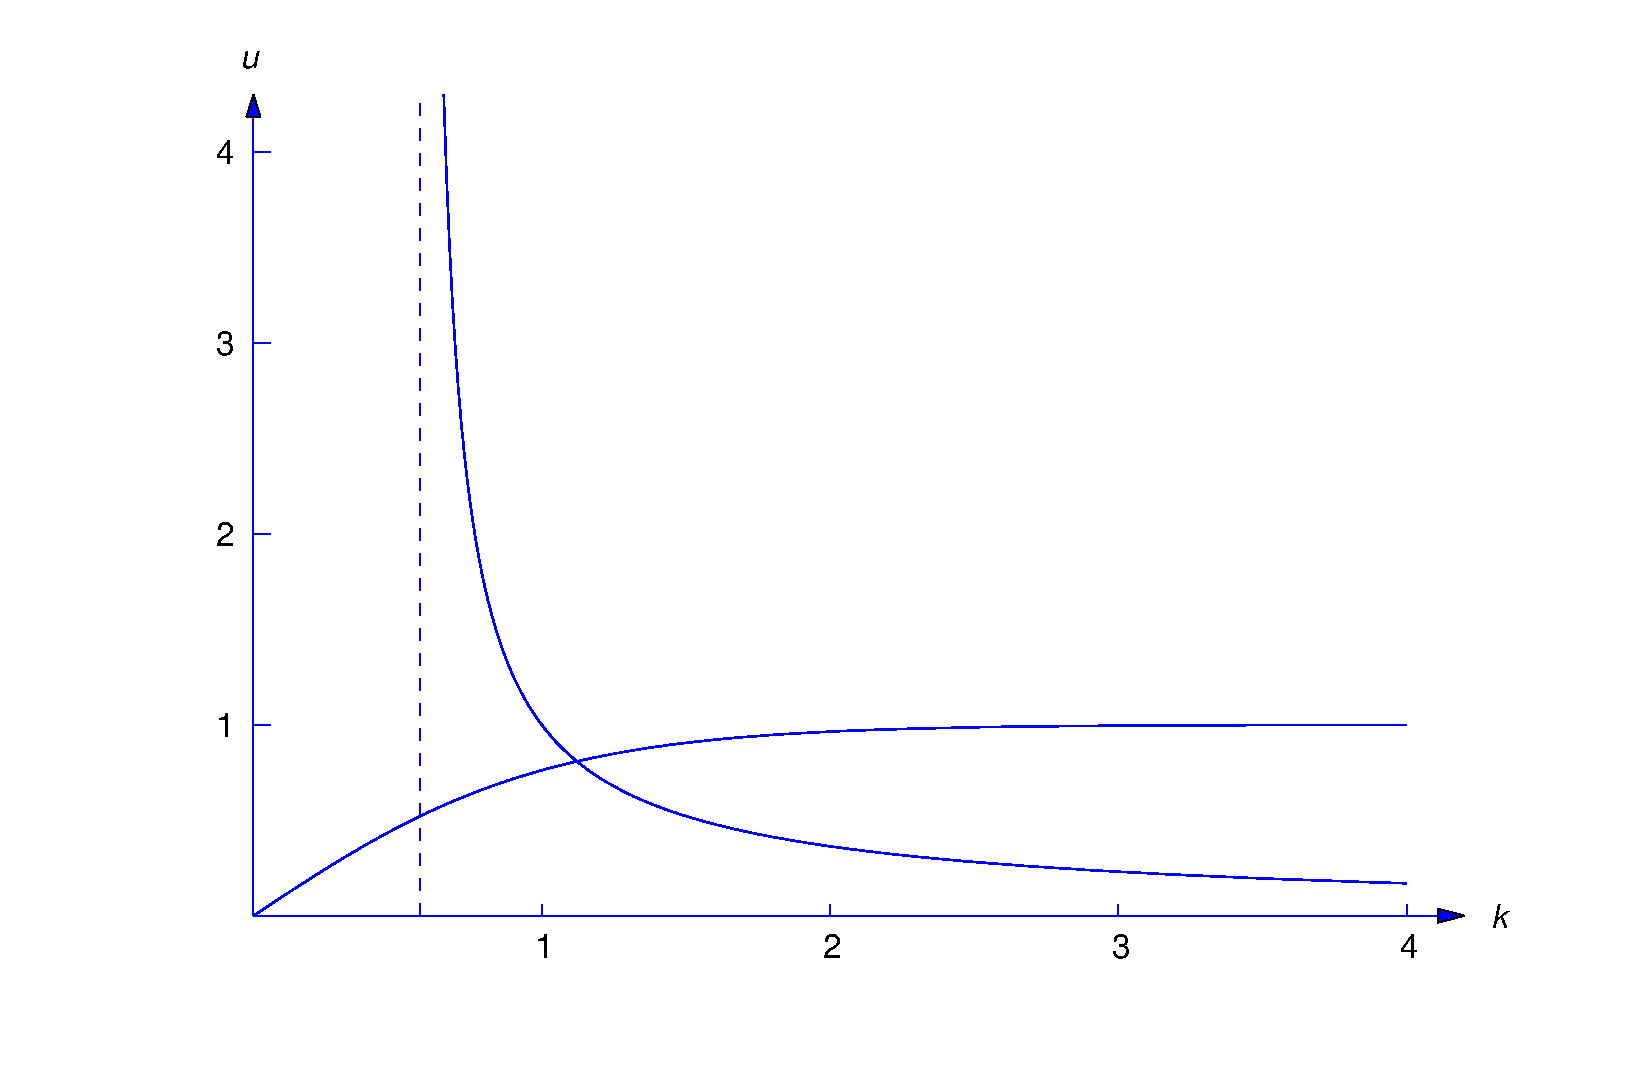
\includegraphics[bb=-78 148 689 643, width=5.67in, height=3.66in, keepaspectratio]{fig130201}
  \caption{$u=\tanh k$ and $u=-2k/(1-3k^{2})$}
  \label{figure:13.2.1}
\end{figure}

If $\lambda>0$ we write $\lambda=k^{2}$ where $k>0$, and differential equation in \eqref{eq:13.2.15}
becomes $y''+k^{2}y=0$, with general solution
\begin{equation}
  \label{eq:13.2.19}y= c_{1}\cos kx+c_{2}\sin kx,
\end{equation}
so
\[
  y'=k(-c_{1}\sin kx+c_{2}\cos kx).
\]
The boundary conditions require that
\begin{equation}
  \label{eq:13.2.20}
  \begin{gathered}
    c_{1}+kc_{2}=0\\ (\cos k-3k\sin k)c_{1}+(\sin k+3k\cos k)c_{2}=0.
  \end{gathered}
\end{equation}
The determinant of this system is
\begin{eqnarray*}
  D_{P}(k)&=& \left|
  \begin{array}{cccccc}
    1               & k               \\
    \cos k-3k\sin k & \sin k+3k\cos k
  \end{array}\right|\\ &=&(1+3k^{2})\sin k+2k\cos k.
\end{eqnarray*}
The system \eqref{eq:13.2.20} has a nontrivial solution if and only if $D_{P}(k)=0$ or,
equivalently,
\[
  \tan k=-\frac{2k}{1+3k^{2}}.
\]
Figure~\ref{figure:13.2.2} shows the graphs of the two sides of this equation. You can see from the
figure that the graphs intersect at infinitely many points $k_{n}\approx n\pi$ ($n=1$, $2$,
$3$,\dots), where the error in this approximation approaches zero as $n\to\infty$. Given this
estimate, you can use Newton's method to compute $k_{n}$ more accurately. We computed
\begin{eqnarray*}
  k_{1} & \approx & \phantom{1}2.9256856, \\
  k_{2} & \approx & \phantom{1}6.1765914, \\
  k_{3} & \approx & \phantom{1}9.3538959, \\
  k_{4} & \approx & 12.5132570.
\end{eqnarray*}
The estimates of the corresponding eigenvalues $\lambda_{n}=k_{n}^{2}$ are
\begin{eqnarray*}
  \lambda_{1} & \approx & \phantom{15}8.5596361, \\
  \lambda_{2} & \approx & \phantom{5}38.1502809, \\
  \lambda_{3} & \approx & \phantom{5}87.4953676, \\
  \lambda_{4} & \approx & 156.5815998.
\end{eqnarray*}
From \eqref{eq:13.2.19} and the first equation in \eqref{eq:13.2.20},
\[
  y_{n}=k_{n}\cos k_{n}x-\sin k_{n}x
\]
is an eigenfunction associated with $\lambda_{n}$ \bbox

\begin{figure}[H]
  \centering
  \relax
  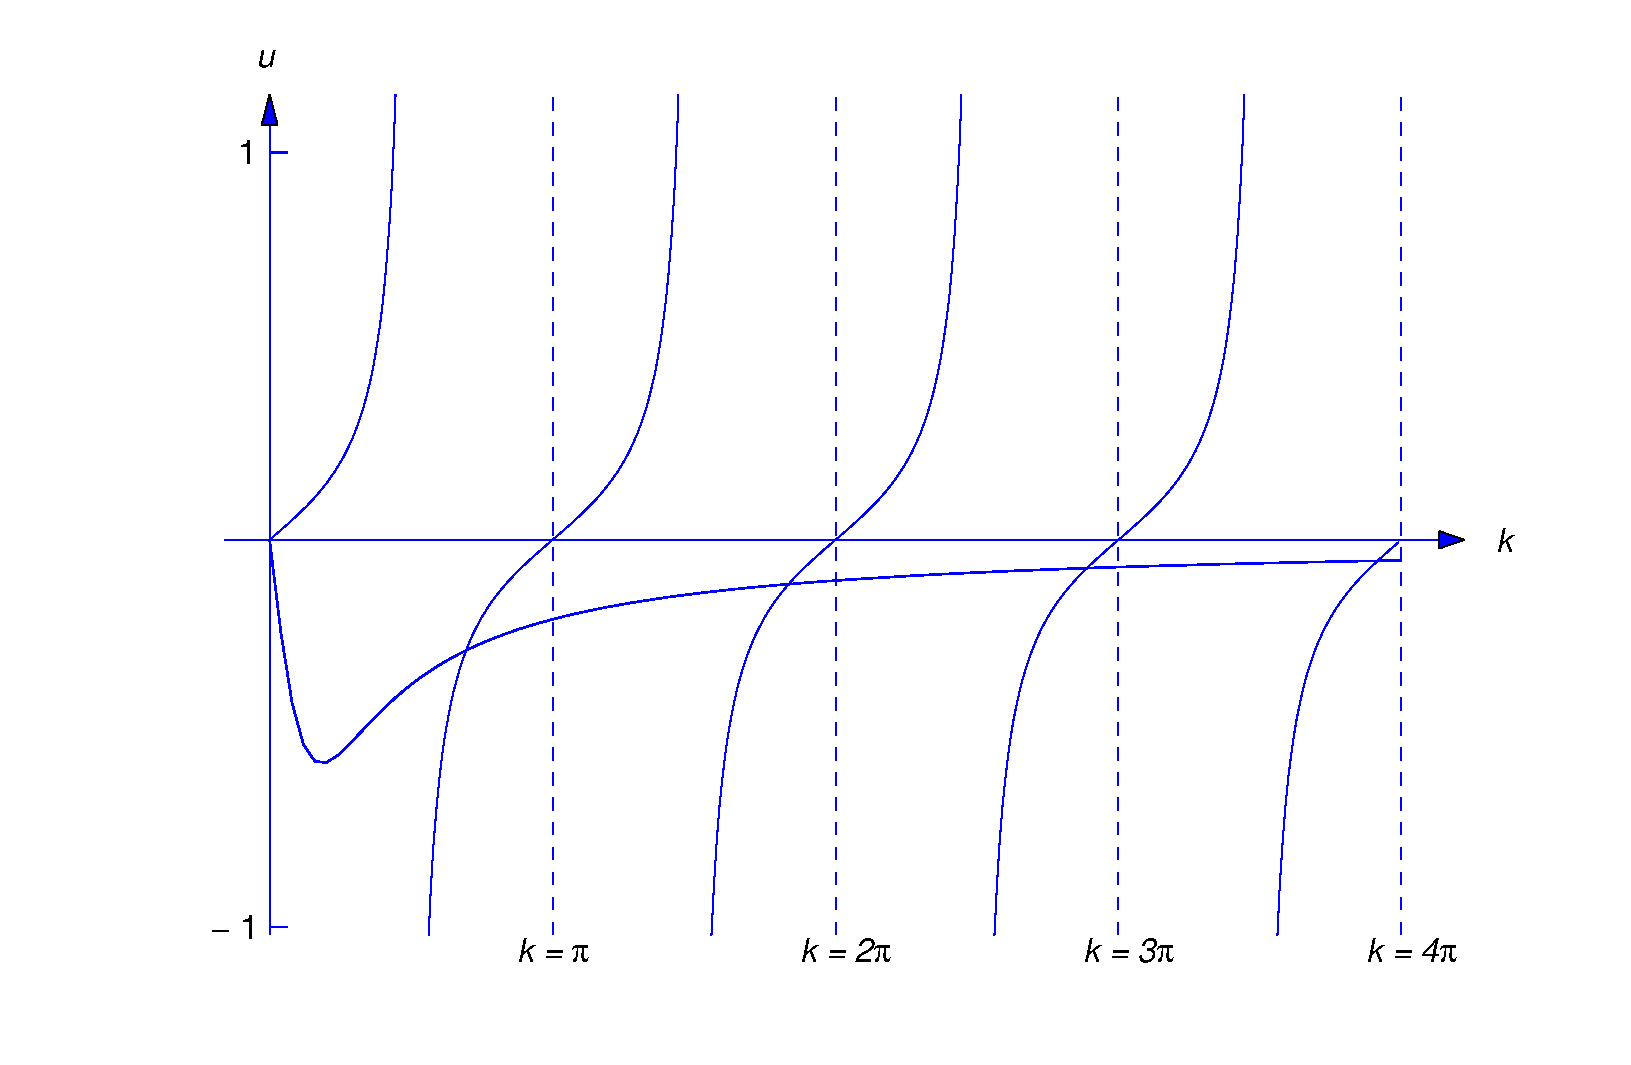
\includegraphics[bb=-78 148 689 643, width=5.67in, height=3.66in, keepaspectratio]{fig130202}
  \caption{$u=\tan k$ and $u=-2k/(1+3k^{2})$}
  \label{figure:13.2.2}
\end{figure}
\end{examplesolution}

\end{document}
